\section{Group Heating and Cooling Coils}\label{group-heating-and-cooling-coils}

Several different coils may be added to zone equipment and air loops. This includes simple heating (gas, electric, and hot water) and a simple water-cooling coil as well as a more detailed flat fin water-cooling coil model. In general, the heating coil description can be used for a heating coil, a reheat coil, or a preheat coil in the air loop simulation or for zone equipment. Figure~\ref{fig:example-air-loop-heating-cooling-coil} is an example of a heating and cooling coil in the air loop simulation in a dual duct system. This does show the basic node structure that will be referenced in the input description. The figure does show water coils since they are the most complex to input in the simulation compared to the Electric and Gas coils which only have air connections.

\begin{figure}[hbtp] % fig 135
\centering
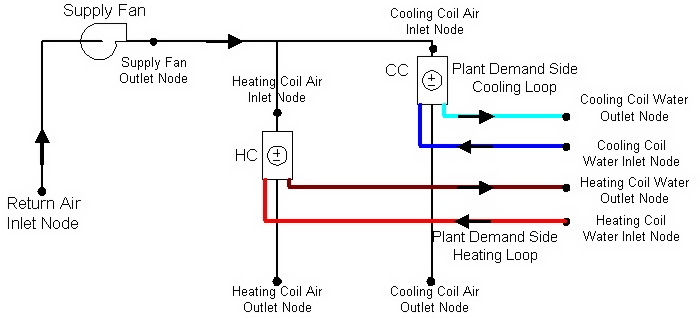
\includegraphics[width=0.9\textwidth, height=0.9\textheight, keepaspectratio=true]{media/image349.png}
\caption{Example Air Loop Heating \& Cooling Coil \protect \label{fig:example-air-loop-heating-cooling-coil}}
\end{figure}

\subsection{Coil:Cooling:Water}\label{coilcoolingwater}

The water cooling coil (Coil:Cooling:Water) has the ability to give detailed output with simplified inputs, inputting complicated coil geometry is not required by the user for this model instead the coil is sized in terms of auto-sizeable thermodynamic inputs. The coil requires thermodynamic inputs such as temperatures, mass flow rates and humidity ratios.

The coil is sized using auto-sized/user design input conditions and the UA values are calculated from the design conditions. A rough estimate of the coil area is provided along with percentage of surface wet and/or dry. This model uses the NTU-effectiveness approach to model heat transfer and has two types of flow arrangements cross-flow or counter-flow.

The basic underlying idea is - use auto sizable thermodynamic design inputs, calculate the coil UA s, use these UA values and operating conditions from the nodes connections, calculate the outlet stream conditions, and calculate the heat transfer rates.

See section Cooling Coil Model in the EnergyPlus Engineering Document for further details regarding this model.

\subsubsection{Inputs}\label{inputs-022}

\paragraph{Field: Name}\label{field-name-021}

A unique user-assigned name for an instance of a cooling coil. Any reference to this cooling coil by another object will use this name.

\paragraph{Field:Availability Schedule Name}\label{fieldavailability-schedule-name-000}

Schedule that defines when the coil is available. The name of the schedule (ref: Schedule) that denotes whether the cooling coil can run during a given time period. A schedule value greater than 0 (usually 1 is used) indicates that the unit can be on during a given time period. A value less than or equal to 0 (usually 0 is used) denotes that the unit is off. If this field is blank, the schedule has a value of 1 for all time periods.

\paragraph{Field: Design Water Flow Rate}\label{field-design-water-flow-rate-000}

The maximum possible water volume flow rate (m\(^{3}\)/sec) through the coil. This is an auto sizable design input.

\paragraph{Field: Design Air Flow Rate}\label{field-design-air-flow-rate-000}

The maximum possible air volume flow rate (m\(^{3}\)/sec) through the coil. This is an auto sizable design input.

\paragraph{Field: Design Inlet Water Temperature}\label{field-design-inlet-water-temperature-000}

The inlet water temperature for the design flow (C). This is an auto sizable design input.

\paragraph{Field: Design Inlet Air Temperature}\label{field-design-inlet-air-temperature}

The inlet air temperature for the design flow (C). This is an auto sizable design input.

\paragraph{Field: Design Outlet Air Temperature}\label{field-design-outlet-air-temperature}

The outlet air condition desired for design flow (C). This is an auto sizable design input.

\paragraph{Field: Design Inlet Air Humidity Ratio}\label{field-design-inlet-air-humidity-ratio}

The highest value of humidity ratio possible for the Design inlet air stream (kgWater/kgDryAir). This is an auto sizable input.

\paragraph{Field: Design Outlet Air Humidity Ratio}\label{field-design-outlet-air-humidity-ratio}

The value of humidity ratio for the Design outlet air stream (kgWater/kgDryAir), it is an auto sizable input.

\paragraph{Field: Water Inlet Node Name}\label{field-water-inlet-node-name-000}

The name of the water coil inlet from the chilled water loop, i.e. Cooling Coil Water Inlet Node. It is from this node the operating inputs for water are transferred to the coil.

\paragraph{Field: Water Outlet Node Name}\label{field-water-outlet-node-name-000}

The name of the water coil outlet from the chilled water loop, i.e. Cooling Coil Water Outlet Node. It is from this node the operating output for water are reported to the coil.

\paragraph{Field: Air Inlet Node Name}\label{field-air-inlet-node-name-003}

The name of the air inlet to the water coil, i.e. Cooling Coil Air Inlet Node. It is from this node the operating inputs for air are transferred to the coil.

\paragraph{Field: Air Outlet Node Name}\label{field-air-outlet-node-name-003}

The name of the air outlet from the water coil, i.e. Cooling Coil Air Outlet Node. It is from this node the operating output for airside is reported to the coil.

\paragraph{Field: Type of Analysis}\label{field-type-of-analysis}

The coil has two modes of operation, termed as \textbf{SimpleAnalysis} and \textbf{DetailedAnalysis}. The difference between the two modes being, the simple mode reports the value of surface area fraction wet of the coil as dry or wet. The detailed mode give the exact value, however the execution time in detailed mode is noticeably higher.

\paragraph{Field: Heat Exchanger Configuration}\label{field-heat-exchanger-configuration-000}

The coil is operable in two configurations: \textit{CounterFlow} or \textit{CrossFlow}. Chilled water coils are generally built as counter-flow. The default is CounterFlow. The detailed NTU-Effectiveness relationships for each flow setting are described in the Engineering Reference, Section `Effectiveness Equations' in `Simulation Models - Encyclopedic Reference: Coil' chapter.

\paragraph{Field: Condensate Collection Water Storage Tank Name}\label{field-condensate-collection-water-storage-tank-name}

This field is optional. It is used to describe where condensate from the coil is collected. If blank or omitted, then any coil condensate is discarded. Enter the name of Water Storage Tank object defined elsewhere and the condensate will then be collected in that tank.

\paragraph{Field: Design Water Temperature Difference}

This input field is optional. If specified, it is used for sizing the \textit{Design Water Flow Rate}. If blank or omitted, the \textit{Loop Design Temperature Difference} value specified in \textit{\hyperref[sizingplant]{Sizing:Plant}} object is used for sizing the \textit{Design Water Flow Rate}.

Examples when auto sized in an IDF are as below:

\begin{lstlisting}

Coil:Cooling:Water,
  Main Cooling Coil 1,       !- Coil Name
  CoolingCoilAvailSched,   !-Availability Schedule Name
  autosize,         !- Design Water Volume Flow Rate of Coil {m3/s}
  autosize,         !- Design Air Flow Rate of Coil {m3/s}
  autosize,         !- Design Inlet Water Temperature {C}
  autosize,         !- Design Inlet Air Temperature {C}
  autosize,         !- Design Outlet Air Temperature {C}
  autosize,         !- Design Inlet Air Humidity Ratio(kgWater/kgDryAir)
  autosize,         !- Design Outlet Air Humidity Ratio(kgWater/kgDryAir)
  Main Cooling Coil 1 Water Inlet Node,     !- Coil_Water_Inlet_Node
  Main Cooling Coil 1 Water Outlet Node,   !- Coil_Water_Outlet_Node
  Mixed Air Node 1,                                             !- Coil_Air_Inlet_Node
  Main Cooling Coil 1 Outlet Node;               !- Coil_Air_Outlet_Node
\end{lstlisting}

Examples when values (hard-sized) are input in an IDF are as below:

\begin{lstlisting}

Coil:Cooling:Water,
  Main Cooling Coil 1,       !- Coil Name
  CoolingCoilAvailSched,   !-Availability Schedule Name
  0.0022,       !- Design Water Volume Flow Rate of Coil {m3/s}
  1.45,           !- Design Air Flow Rate of Coil {m3/s}
  6.1,             !- Design Inlet Water Temperature {C}
  25,               !- Design Inlet Air Temperature {C}
  10,               !- Design Outlet Air Temperature {C}
  0.012,         !- Design Inlet Air Humidity Ratio
  0.008,         !- Design Outlet Air Humidity Ratio
  Main Cooling Coil 1 Water Inlet Node,     !- Coil_Water_Inlet_Node
  Main Cooling Coil 1 Water Outlet Node,   !- Coil_Water_Outlet_Node
  Mixed Air Node 1,                                             !- Coil_Air_Inlet_Node
  Main Cooling Coil 1 Outlet Node;               !- Coil_Air_Outlet_Node
\end{lstlisting}

\subsubsection{Outputs}\label{outputs-015}

Following are the list of possible output variables from this coil model:

\begin{itemize}
\item
  HVAC,Sum,Cooling Coil Total Cooling Energy {[}J{]}
\item
  HVAC,Sum,Cooling Coil Sensible Cooling Energy {[}J{]}
\item
  HVAC,Average,Cooling Coil Total Cooling Rate {[}W{]}
\item
  HVAC,Average,Cooling Coil Sensible Cooling Rate {[}W{]}
\item
  HVAC,Average,Cooling Coil Wetted Area Fraction {[]}
\item
  HVAC,Average,Cooling Coil Condensate Volume Flow Rate {[}m3/s{]}
\item
  HVAC,Sum,Cooling Coil Source Side Heat Transfer Energy {[}J{]}
\item
  HVAC,Sum,Cooling Coil Condensate Volume {[}m3{]}
\end{itemize}

\paragraph{Cooling Coil Total Cooling Energy (J)}\label{cooling-coil-total-cooling-energy-j}

Cooling Coil Total Cooling Energy is the total amount of heat transfer taking place in the coil at the operating conditions.

\paragraph{Cooling Coil Sensible Cooling Energy (J)}\label{cooling-coil-sensible-cooling-energy-j}

Cooling Coil Sensible Cooling Energy is the total amount of Sensible heat transfer taking place in the coil at the operating conditions. It only takes into account temperature difference in the inlet and outlet air streams at operating conditions.

\paragraph{Cooling Coil Total Cooling Rate (W)}\label{cooling-coil-total-cooling-rate-w}

Cooling Coil Total Cooling Rate is the Rate of heat transfer taking place in the coil at the operating conditions. The units are (J/sec) or Watts.

\paragraph{Cooling Coil Sensible Cooling Rate (W)}\label{cooling-coil-sensible-cooling-rate-w}

Cooling Coil Sensible Cooling Rate is the Rate of Sensible heat transfer taking place in the coil at the operating conditions.

\paragraph{Cooling Coil Wetted Area Fraction {[]}}\label{cooling-coil-wetted-area-fraction}

It defines the fraction of total surface area of coil which is wet due to moisture condensation on the surface of the coil. Value varies between 0.0 and 1.0.

In addition, if a Water Storage Tank is used to collect coil condensate, then the following outputs will be available.

\paragraph{Cooling Coil Condensate Volume Flow Rate {[}m3/s{]}}\label{cooling-coil-condensate-volume-flow-rate-m3s}

\paragraph{Cooling Coil Condensate Volume {[}m3{]}}\label{cooling-coil-condensate-volume-m3}

These reports provide the rate and amount of condensate from the coil. Condensate is water condensed out of the air as a result of cooling. The condensate volume is also reported on the meter for OnSiteWater.

\paragraph{Cooling Coil Source Side Heat Transfer Energy {[}J{]}}\label{cooling-coil-source-side-heat-transfer-energy-j}

This is the energy extracted from the chilled water serving the coil, in Joules.


\subsection{Coil:Cooling:Water:DetailedGeometry}\label{coilcoolingwaterdetailedgeometry}

This detailed flat fin coil model is for continuous plate fins. First, found in Type 12 from MODSIM, but now programmed directly from Elmahdy, A.H. and Mitalas, G.P. Then there was a discontinuity in their original model that was fixed in the EnergyPlus implementation. Now this model can be used in an interval halving solution technique for controlling this coil without the problems of non-convergence.

``A Model for Cooling and Dehumidifying Coils for Use in Energy Requirements for Buildings'' ASHRAE Transactions, Vol. 83, Part 2, pp.~103-117 (1977). For fin efficiency see K.A. Gardner, ``Efficiency of Extended ,'' Transactions ASME, Vol. 67, pp.~621-631, 1945.

The following figures illustrate the geometry and circuits in a cooling coil.

\begin{figure}[hbtp] % fig 136
\centering
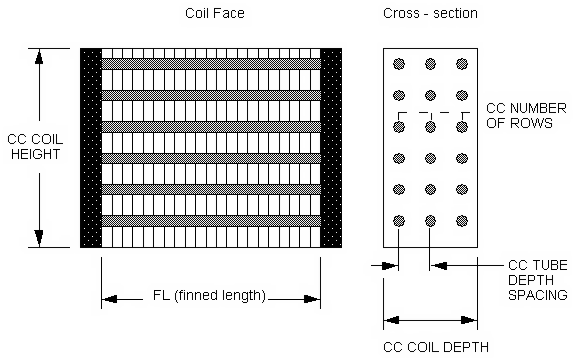
\includegraphics[width=0.9\textwidth, height=0.9\textheight, keepaspectratio=true]{media/image353.png}
\caption{Geometry of a Cooling Coil (CC) \protect \label{fig:geometry-of-a-cooling-coil-cc}}
\end{figure}

\begin{figure}[hbtp] % fig 137
\centering
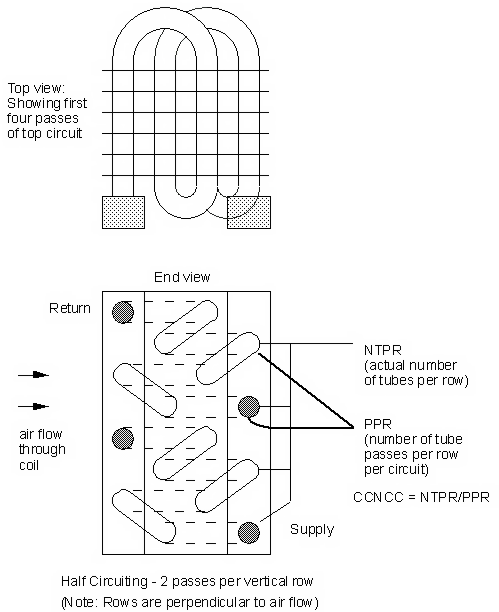
\includegraphics[width=0.9\textwidth, height=0.9\textheight, keepaspectratio=true]{media/image354.png}
\caption{Number of Coolant Circuits (CCNCC) \protect \label{fig:number-of-coolant-circuits-ccncc}}
\end{figure}

\subsubsection{Inputs}\label{inputs-12-005}

\paragraph{Field: Name}\label{field-name-11-004}

A unique identifying name for each coil.

\paragraph{Field:Availability Schedule Name}\label{fieldavailability-schedule-name-5}

Schedule that defines when the coil is available. If the schedule's value is 0.0, then the coil is not available and flow will not be requested. If the schedule's value is \textgreater{} 0.0 (usually 1 is used), the coil is available. If this field is blank, the schedule has values of 1 for all time periods.

\paragraph{Field: Maximum Water Flow Rate}\label{field-maximum-water-flow-rate-1}

The maximum possible water flow rate (m\(^{3}\)/sec) through the coil.

\paragraph{Field: Tube Outside Surface Area}\label{field-tube-outside-surface-area}

The outside surface area (m\(^{2}\)) of the tubes that is exposed to air (i.e. the outside area of the unfinned tubes minus the area of tubes covered by the fins).

\paragraph{Field: Total Tube Inside Area}\label{field-total-tube-inside-area}

The total surface area (m\(^{2}\)) inside the tubes (water side).

\paragraph{Field: Fin Surface Area}\label{field-fin-surface-area}

The total surface area (m\(^{2}\)) of the fins attached to the coil.

\paragraph{Field: Minimum Air Flow Area}\label{field-minimum-air-flow-area}

The minimum cross sectional area (m\(^{2}\)) available for air passage. Frequently calculated as

\begin{lstlisting}
       Amin  = (Amin/Afr)\*Afr
\end{lstlisting}

where Afr is the frontal area of the heat exchanger, and (Amin/Afr) is the ratio of the minimum airflow area to frontal area.

\paragraph{Field: Coil Depth}\label{field-coil-depth}

The distance (m) from the front of the coil to the back of the coil in the airflow direction. Also called the fin depth. Illustrated in the figure (Figure~\ref{fig:geometry-of-a-cooling-coil-cc}. Geometry of a Cooling Coil (CC)).

\paragraph{Field: Fin Diameter}\label{field-fin-diameter}

The outside diameter (m) of the fins. Used instead of COIL HEIGHT

\paragraph{Field: Fin Thickness}\label{field-fin-thickness}

Thickness (m) of the air side fins.

\paragraph{Field: Tube Inside Diameter}\label{field-tube-inside-diameter}

The inside diameter (m) of the tubes.

\paragraph{Field: Tube Outside Diameter}\label{field-tube-outside-diameter}

The outside diameter (m) of the tubes.

\paragraph{Field: Tube Thermal Conductivity}\label{field-tube-thermal-conductivity}

The thermal conductivity (W/m-K) of the tube material.

\paragraph{Field: Fin Thermal Conductivity}\label{field-fin-thermal-conductivity}

The thermal conductivity (W/m-K) of the fin material.

\paragraph{Field: Fin Spacing}\label{field-fin-spacing}

The spacing (m) of the fins, centerline to centerline.

\paragraph{Field: Tube Depth Spacing}\label{field-tube-depth-spacing}

The spacing (m) of the tube rows, centerline to centerline. Also called tube longitudinal spacing.

\paragraph{Field: Number of Tube Rows}\label{field-number-of-tube-rows}

The number of tube rows in the direction of the airflow.

\paragraph{Field: Number of Tubes per Row}\label{field-number-of-tubes-per-row}

The number of tubes per row. (NTPR in the above diagram)

\paragraph{Field: Water Inlet Node Name}\label{field-water-inlet-node-name-3-000}

The name of the water coil inlet from the chilled water loop, i.e. Cooling Coil Water Inlet Node.

\paragraph{Field: Water Outlet Node Name}\label{field-water-outlet-node-name-3-000}

The name of the water coil outlet from the chilled water loop, i.e. Cooling Coil Water Outlet Node.

\paragraph{Field: Air Inlet Node Name}\label{field-air-inlet-node-name-8}

The name of the air inlet to the water coil, i.e. Cooling Coil Air Inlet Node.

\paragraph{Field: Air Outlet Node Name}\label{field-air-outlet-node-name-8-000}

The name of the air outlet from the water coil, i.e. Cooling Coil Air Outlet Node.

\paragraph{Field: Condensate Collection Water Storage Tank Name}\label{field-condensate-collection-water-storage-tank-name-1}

This field is optional. It is used to describe where condensate from the coil is collected. If blank or omitted, then any coil condensate is discarded. Enter the name of Water Storage Tank object defined elsewhere and the condensate will then be collected in that tank.

\paragraph{Field: Design Water Temperature Difference}\label{field-design-water-temperature-difference}

This input field is optional. If specified, it is used for sizing the \textit{Design Water Flow Rate}. If blank or omitted, the \textit{Loop Design Temperature Difference} value specified in \textit{\hyperref[sizingplant]{Sizing:Plant}} object is used for sizing the \textit{Design Water Flow Rate}.

\paragraph{Field: Design Water Inlet Temperature}\label{field-design-water-inlet-temperature}

This input field is optional. If specified, it is used for sizing the coil \textit{Design Geometry Parameters}. If blank or omitted, the \textit{Design Loop Exit Temperature} value specified in \textit{\hyperref[sizingplant]{Sizing:Plant}} object is used for sizing the coil \textit{Design Geometry Parameters}.

Examples of these statements in an IDF are:

\begin{lstlisting}

Coil:Cooling:Water:DetailedGeometry,
  Detailed Cooling Coil,   !Name of cooling coil
  CoolingCoilAvailSched,   !Cooling Coil Schedule
  0.0011,                   !Max Water Flow Rate of Coil m3/sec
  6.23816,                 !Tube Outside Surf Area
  6.20007018,           !Tube Inside Surf Area
  101.7158224,         !Fin Surf Area
  0.300606367,         !Min Air Flow Area
  0.165097968,         !Coil Depth
  0.43507152,           !Coil Height
  0.001499982,         !Fin Thickness
  0.014449958,         !Tube Inside Diameter
  0.015879775,         !Tube Outside Diameter
  386.0,                     !Tube Thermal Conductivity
  204.0,                     !Fin Thermal Conductivity
  0.001814292,         !Fin Spacing
  0.02589977,           !Tube Depth
  6,                             !Number of Tube Rows
  16,                           !Number of Tubes per Row
  NODE_32,NODE_33, !Coil Water Side Inlet & Outlet Node
  NODE_5, NODE_6;   !Coil Air Side Inlet & Outlet Node
\end{lstlisting}

\subsubsection{Outputs}\label{outputs-11-002}

\begin{itemize}
\item
  HVAC,Sum,Cooling Coil Total Cooling Energy {[}J{]}
\item
  HVAC,Sum,Cooling Coil Sensible Cooling Energy {[}J{]}
\item
  HVAC,Average,Cooling Coil Total Cooling Rate {[}W{]}
\item
  HVAC,Average,Cooling Coil Sensible Cooling Rate {[}W{]}
\item
  HVAC,Average,Cooling Coil Condensate Volume Flow Rate {[}m3/s{]}
\item
  HVAC,Sum,Cooling Coil Source Side Heat Transfer Energy {[}J{]}
\item
  HVAC,Sum,Cooling Coil Condensate Volume {[}m3{]}
\end{itemize}

\paragraph{Cooling Coil Total Cooling Energy (J)}\label{cooling-coil-total-cooling-energy-j-3}

Cooling Coil Total Cooling Energy is the total amount of heat transfer taking place in the coil at the operating conditions.

\paragraph{Cooling Coil Sensible Cooling Energy (J)}\label{cooling-coil-sensible-cooling-energy-j-3}

Cooling Coil Sensible Cooling Energy is the total amount of Sensible heat transfer taking place in the coil at the operating conditions. It only takes into account temperature difference in the inlet and outlet air streams at operating conditions.

\paragraph{Cooling Coil Total Cooling Rate (W)}\label{cooling-coil-total-cooling-rate-w-3}

Cooling Coil Total Cooling Rate is the Rate of heat transfer taking place in the coil at the operating conditions. The units are (J/sec) or Watts.

\paragraph{Cooling Coil Sensible Cooling Rate (W)}\label{cooling-coil-sensible-cooling-rate-w-3}

Cooling Coil Sensible Cooling Rate is the Rate of Sensible heat transfer taking place in the coil at the operating conditions.

In addition, if a Water Storage Tank is used to collect coil condensate, then the following outputs will be available.

\paragraph{Cooling Coil Condensate Volume Flow Rate {[}m3/s{]}}\label{cooling-coil-condensate-volume-flow-rate-m3s-3}

\paragraph{Cooling Coil Condensate Volume {[}m3{]}}\label{cooling-coil-condensate-volume-m3-3}

These reports provide the rate and amount of condensate from the coil. Condensate is water condensed out of the air as a result of cooling. The condensate volume is also reported on the meter for OnSiteWater.

\paragraph{Cooling Coil Source Side Heat Transfer Energy {[}J{]}}\label{cooling-coil-source-side-heat-transfer-energy-j-1}

This is the energy extracted from the chilled water serving the cooling coil, in Joules.

\subsection{CoilSystem:Cooling:Water:HeatExchangerAssisted}\label{coilsystemcoolingwaterheatexchangerassisted}

The heat exchanger-assisted water cooling coil is a virtual component consisting of a chilled-water cooling coil and an air-to-air heat exchanger as shown in Figure~\ref{fig:schematic-of-the-coilsystem-cooling-water} below. The air-to-air heat exchanger precools the air entering the cooling coil, and reuses this energy to reheat the supply air leaving the cooling coil. This heat exchange process improves the latent removal performance of the cooling coil by allowing it to dedicate more of its cooling capacity toward dehumidification (lower sensible heat ratio).

\begin{figure}[hbtp] % fig 140
\centering
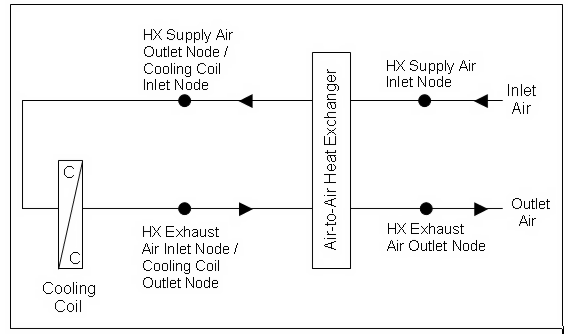
\includegraphics[width=0.9\textwidth, height=0.9\textheight, keepaspectratio=true]{media/image370.png}
\caption{Schematic of the CoilSystem:Cooling:Water:HeatExchangerAssisted compound object \protect \label{fig:schematic-of-the-coilsystem-cooling-water}}
\end{figure}

Note: Node naming shown in Figure~\ref{fig:schematic-of-the-coilsystem-cooling-water} is representative for \hyperref[heatexchangerairtoairsensibleandlatent]{HeatExchanger:AirToAir:SensibleAndLatent}. For \hyperref[heatexchangerairtoairflatplate]{HeatExchanger:AirToAir:FlatPlate}, the exhaust air nodes are referred to as secondary air nodes.

This compound object models the basic operation of an air-to-air heat exchanger in conjunction with a chilled-water cooling coil. The heat exchanger-assisted water cooling coil does not have an operating schedule of its own; its operating schedule is governed by the availability schedules for the chilled-water cooling coil and the air-to-air heat exchanger. Heat exchange will occur whenever the heat exchanger is available to operate (via its availability schedule) and a temperature difference exists between the two air streams -- there is currently no method to enable or disable heat exchange based on zone air humidity level. This compound object is used in place of where a chilled-water cooling coil object would normally be used by itself.

To model a heat exchanger-assisted water cooling coil, the input data file should include the following objects:

\begin{itemize}
\item
  CoilSystem:Cooling:Water:HeatExchangerAssisted compound object
\item
  Air-to-air heat exchanger object (\hyperref[heatexchangerairtoairflatplate]{HeatExchanger:AirToAir:FlatPlate} or \hyperref[heatexchangerairtoairsensibleandlatent]{HeatExchanger:AirToAir:SensibleAndLatent})
\item
  Chilled-water cooling coil object (\hyperref[coilcoolingwater]{Coil:Cooling:Water} or \hyperref[coilcoolingwaterdetailedgeometry]{Coil:Cooling:Water:DetailedGeometry})
\end{itemize}

Links to the cooling coil and air-to-air heat exchanger specifications are provided in the input data syntax for this compound object. A description of each input field for this compound object is provided below.

\subsubsection{Inputs}\label{inputs-26}

\paragraph{Field: Name}\label{field-name-25-000}

A unique user-assigned name for the heat exchanger-assisted water cooling coil. Any reference to this compound component by another object (e.g., \hyperref[zonehvacunitventilator]{ZoneHVAC:UnitVentilator}, \hyperref[zonehvacfourpipefancoil]{ZoneHVAC:FourPipeFanCoil}, component in an air loop Branch object) will use this name.

\paragraph{Field: Heat Exchanger Object Type}\label{field-heat-exchanger-object-type-1}

This alpha field denotes the type of heat exchanger being modeled. Valid choices are:

\hyperref[heatexchangerairtoairflatplate]{HeatExchanger:AirToAir:FlatPlate}

\hyperref[heatexchangerairtoairsensibleandlatent]{HeatExchanger:AirToAir:SensibleAndLatent}

\paragraph{Field: Heat Exchanger Name}\label{field-heat-exchanger-name-1}

This alpha field denotes the name of the air-to-air heat exchanger being modeled.

\paragraph{Field: Cooling Coil Object Type}\label{field-cooling-coil-object-type-2}

This alpha field denotes the type of chilled-water cooling coil being modeled. Valid choices are:

\hyperref[coilcoolingwater]{Coil:Cooling:Water}

\hyperref[coilcoolingwaterdetailedgeometry]{Coil:Cooling:Water:DetailedGeometry}

\paragraph{Field: Cooling Coil Name}\label{field-cooling-coil-name-2}

This alpha field denotes the name of the chilled-water cooling coil being modeled.

Following is an example input for this compound object:

\begin{lstlisting}

CoilSystem:Cooling:Water:HeatExchangerAssisted,
  Heat Exchanger Assisted Cooling Coil 1, !- Name of the heat exchanger assisted cooling coil
  HeatExchanger:AirToAir:FlatPlate,     !- Heat exchanger type
  Heat Exchanger Assisting Cooling Coil,   !- Heat exchanger name
  Coil:Cooling:Water:DetailedGeometry,                 !- Cooling coil type
  Main Cooling Coil 1;                                       !- Cooling coil name


  HeatExchanger:AirToAir:FlatPlate,
  Heat Exchanger Assisting Cooling Coil,   !- Name
  CoolingCoilAvailSched,     !- Availability Schedule Name
  Counter Flow,                       !- flow arrangement
  Yes,                                         !- Economizer lockout
  1.0,                                         !- hA ratio
  1.32,                                       !- Nominal supply air flow rate {m3/s}
  24.0,                                       !- Nominal supply air inlet temperature {C}
  21.0,                                       !- Nominal supply air outlet temperature {C}
  1.32,                                       !- Nominal secondary air flow rate {m3/s}
  12.0,                                       !- Nominal secondary air inlet temperature {C}
  100.0,                                     !- Nominal electric power {W}
  Mixed Air Node 1,               !- Supply air inlet node
  Main Cooling Coil 1 Inlet Node,   !- Supply air outlet node
  Main Cooling Coil 1 Outlet Node, !- Secondary air inlet node
  Main Heating Coil 1 Inlet Node;   !- Secondary air outlet node




  Coil:Cooling:Water:DetailedGeometry,
  Main Cooling Coil 1,         !- Coil Name
  CoolingCoilAvailSched,     !- Availability Schedule Name
  autosize,                               !- Max Water Flow Rate of Coil {m3/s}
  autosize,                               !- Tube Outside Surf Area {m2}
  autosize,                               !- Total Tube Inside Area {m2}
  autosize,                               !- Fin Surface Area {m2}
  autosize,                               !- Minimum Air Flow Area {m2}
  autosize,                               !- Coil Depth {m}
  autosize,                               !- Fin Diameter {m}
  ,                                               !- Fin Thickness {m}
  ,                                               !- Tube Inside Diameter {m}
  ,                                               !- Tube Outside Diameter {m}
  ,                                               !- Tube Thermal Conductivity {W/m-K}
  ,                                               !- Fin Thermal Conductivity {W/m-K}
  ,                                               !- Fin Spacing {m}
  ,                                               !- Tube Depth Spacing {m}
  ,                                               !- Number of Tube Rows
  autosize,                               !- Number of Tubes per Row
  Main Cooling Coil 1 Water Inlet Node,   !- Coil_Water_Inlet_Node
  Main Cooling Coil 1 Water Outlet Node, !- Coil_Water_Outlet_Node
  Main Cooling Coil 1 Inlet Node,     !- Coil_Air_Inlet_Node
  Main Cooling Coil 1 Outlet Node;   !- Coil_Air_Outlet_Node
\end{lstlisting}

\subsubsection{Outputs}\label{outputs-22}

No variables are reported for this compound object. However, outputs are provided by the cooling coil and heat exchanger that are specified.

\subsection{CoilSystem:Cooling:Water}\label{coilsystemcoolingwater}

The \hyperref[coilsystemcoolingwater]{CoilSystem:Cooling:Water} object is a coil system wrapper for water cooling coils. Valid water cooling coils are: \hyperref[coilcoolingwater]{Coil:Cooling:Water}, \hyperref[coilcoolingwaterdetailedgeometry]{Coil:Cooling:Water:DetailedGeometry} and \hyperref[coilsystemcoolingwaterheatexchangerassisted]{CoilSystem:Cooling:Water:HeatExchangerAssisted}. This coil system allows users to model the three water cooling coils in airloop main and outdoor air branches. Also this object is designed to model water-side economizers for free pre-cooling when the water-side of the coil is placed on the demand side a condenser loop. As a water-side economizer the \textit{CoilSystem:Cooling:Water} object is placed upstream of packaged DX systems or chilled water main cooling coils. The coil system as a water-side economizer provides free pre-cooling when the condition is favorable. Any remaining system cooling load not met by the water side economizer is provided either by a DX or chilled water cooling coil placed downstream of the water-side economizer coil. The \textit{CoilSystem:Cooling:Water} object does not require \textit{Controller:WaterCoil} and relies on a built-in controller. This coil system uses setpoint based control that varies coil entering water (fluid) mass flow rate to meet user specified temperature or humidity setpoint.\par

Figure~\ref{fig:water-side-economizer-coil-system-upstream-of-packaged-dx-system} below shows packaged DX system serving multiple zones and a coil system water cooling object placed upstream of the packaged system. The water-side of the coil system is connected to the demand side of a condenser or plant loop. This coil system configuration provides free pre-cooling when the condition is favorable to operate and there is cooling or dehumidification demand. In this configuration the packaged DX system can be \textit{AirloopHVAC:UnitarySystem} object.

\begin{figure}[hbtp] % fig 141
\centering
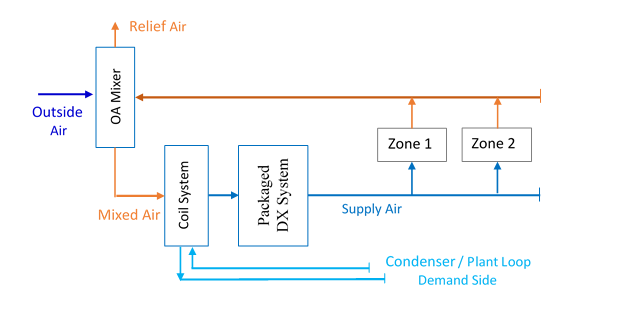
\includegraphics[width=0.9\textwidth, height=0.9\textheight, keepaspectratio=true]{media/image141.png}
\caption{Water Side Economizer Coil System Upstream of Packaged DX System \protect \label{fig:water-side-economizer-coil-system-upstream-of-packaged-dx-system}}
\end{figure}

Figure~\ref{fig:water-side-economizer-coil-system-in-outdoor-air-system} below shows a packaged DX system serving multiple zones and a coil system water cooling object placed in the outdoor air system. The water-side of the coil system is connected to the demand side of a condenser or plant loop.  This coil provides free cooling to the outdoor air stream when the condition is favorable to operate and there is pre-cooling demand.

\begin{figure}[hbtp] % fig 142
\centering
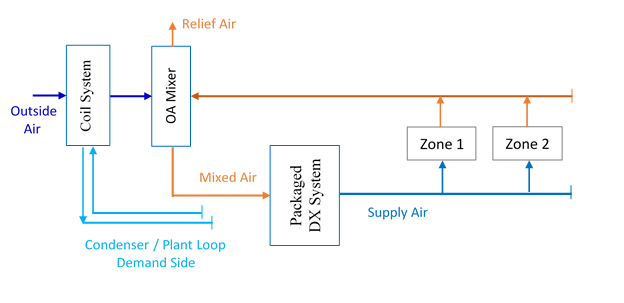
\includegraphics[width=0.9\textwidth, height=0.9\textheight, keepaspectratio=true]{media/image142.png}
\caption{Water Side Economizer Coil System In Outdoor Air System \protect \label{fig:water-side-economizer-coil-system-in-outdoor-air-system}}
\end{figure}


\subsubsection{Water Side Economizer Mode}\label{water-side-economizer-mode}

The coil system cooling object to operate the coil entering water (fluid) temperature must be less than the coil entering air temperature minus the user specified temperature offset value. The second requirement is that the coil system entering air temperature must be greater than the coil system air outlet node (control node) setpoint temperature, i.e., there has to be a cooling or dehumidification demand. Built in coil system controller strives to meet either temperature or humidity ratio setpoint at the coil system air outlet node by varying the cold water (fluid) mass flow rate.

\subsubsection{Wrap Around Water Coil Heat Recovery Mode}\label{wrap-around-water-coil-heat-recovery-mode}

This coil system may also be used to model a wrap-around water coil heat recovery system where a water coil system object is in one air stream (e.g., the outdoor air stream) while another cooling coil object is in a seperate air stream (e.g., exhaust air stream). The two water coils are connected in series on the demand side of a plant loop where the CoilSystem:Cooling:Water object is upstream of the Coil:Cooling:Water object. For wrap-around heat recovery coils, the supply side of the plant will typically have only a pump to circulate the water.\par

The CoilSystemCooling:Water object is the main controller for the heat recovery loop. Neither this object or other coils in the heat recovery loop require an external controller (Ref: \hyperref[controllerwatercoil]{Controller:WaterCoil}). Do not specify a controller for this object or the associated water coil elsewhere in the input. This object checks that the water coil entering water (fluid) temperature to coil entering air temperature absolute difference is greater than the user specified temperature offset, otherwise the system is disabled. The water loop temperature entering the coil system's coil will be maintained between the entering air temperatures of the water coils (e.g., midway between the outdoor air temperature and exhaust air temperature if the coils are used in the outdoor air system). The coil system will be disabled if the plant loop water temperature falls below the minimum allowed heat recovery loop water temperature (Ref. field \hyperref[field-minimum-water-loop-temperature-for-heat-recovery]{Minimum Water Loop Temperature For Heat Recover}). Figure~\ref{fig:wrap-around-water-coil-heat-recovery-system-in-outdoor-air-system} shows a wrap-around heat recovery coil system in the outdoor air and relief air streams of the outdoor air system.

\textbf{Note - although a \hyperref[plantloop]{PlantLoop} temperature setpoint node name and associated set point manager is required, that set point will not be used.} 

\begin{figure}[hbtp] % fig 143
\centering
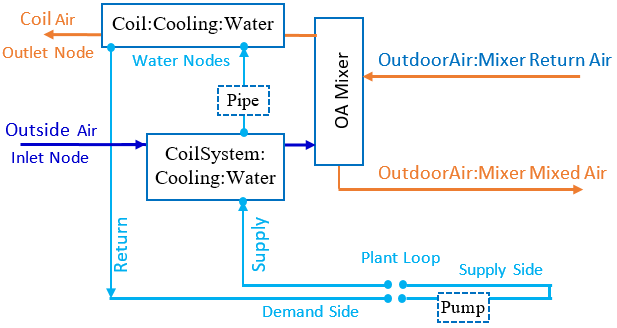
\includegraphics[width=0.9\textwidth, height=0.9\textheight, keepaspectratio=true]{media/CoilSystemWater_HeatRecovery.png}
\caption{Wrap-Around Water Coil Heat Recovery System In Outdoor Air System \protect \label{fig:wrap-around-water-coil-heat-recovery-system-in-outdoor-air-system}}
\end{figure}


\subsubsection{Inputs}\label{inputs}

\paragraph{Field: Name}\label{field-name-06}

This alpha field contains the identifying name for the coil system cooling water object. Any reference to this coil system by another object will use this name.

\paragraph{Field: Air Inlet Node Name}\label{field-air-inlet-node-name-01}

This alpha field contains the coil system cooling water object air inlet node name.

\paragraph{Field: Air Outlet Node Name}\label{field-air-outlet-node-name-01}

This alpha field contains the coil system cooling water object air outlet node name.

\paragraph{Field: Availability Schedule Name}

This alpha field contains the schedule name which contains information on the availability of the coil system cooling water object to operate. A schedule value equal to 0 denotes that the coil system must be off for that time period. A value greater than 0 denotes that the coil system is available to operate during that time period. This schedule may be used to completely disable the coil system as required. If this field is left blank, the schedule has a value of 1.

\paragraph{Field: Cooling Coil Object Type}\label{field-cooling-coil-object-type-01}

This alpha field contains the identifying type of cooling coil specified in the coil system cooling water object. Valid choices for this field are:
\begin{itemize}
\item Coil:Cooling:Water
\item Coil:Cooling:Water:DetailedGeometry
\item CoilSystem:Cooling:Water:HeatExchangerAssisted
\end{itemize}


\paragraph{Field: Cooling Coil Name}\label{field-cooling-coil-name-01}

This alpha field contains the identifying name given to the coil system water cooling coil.

\paragraph{Field: Dehumidification Control Type}

This alpha field contains the type of dehumidification control. The following options are valid for this field:

\textbf{None} - meet sensible load only, no active dehumidification control. Valid with all cooling coil types. When a heat exchanger assisted cooling coil is used, the heat exchanger is locked on at all times. The default is None.

\textbf{Multimode} - activate water coil and meet sensible load. If no sensible load exists, and Run on Latent Load = Yes, and a latent load exists, the coil will operate to meet the latent load. If the latent load cannot be met the heat exchanger will be activated. This control mode allows the heat exchanger to be turned on and off based on the dehumidification setpoint. Valid only with cooling coil type CoilSystem:Cooling:Water:HeatExchangerAssisted.

\textbf{CoolReheat} - cool beyond the dry-bulb temperature set point as required to meet the high humidity setpoint. If cooling coil type = CoilSystem:Cooling:Water:HeatExchangerAssisted, then the heat exchanger is assumed to always transfer energy between the cooling coil’s inlet and outlet airstreams when the cooling coil is operating.


For the dehumidification control modes, the maximum humidity setpoint on the Sensor Node is used. This must be set using a ZoneControl:Humidistat object. When extra dehumidification is required, the system may not be able to meet the humidity setpoint if its full capacity is not adequate. If the dehumidification control type is specified as CoolReheat, then the system may require reheat coil type and name elsewhere. Although the reheat coil is required only when CoolReheat is selected, the optional reheat coil may be present for any of the allowed Dehumidification Control Types.

Valid humidity setpoint managers include:
\begin{itemize}
\item SetpointManager:SingleZone:Humidity:Maximum
\item SetpointManager:MultiZone:Humidity:Maximum
\item SetpointManager:MultiZone:MaximumHumidity:Average
\item SetpointManager:OutdoorAirPretreat
\end{itemize}

\paragraph{Field: Run On Sensible Load}\label{field-run-on-sensible-load-01}

This alpha field specifies if the coil system will operate to meet a sensible load calculated from the air flow rates through the coil system, coil system entering air temperature and coil outlet node (control node) temperature setpoint. There are two valid choices, Yes or No. If Yes, coil will run if there is a sensible load. If No, coil will not run if there is only a sensible load. The default is Yes.


\paragraph{Field: Run on Latent Load}\label{field-run-on-latent-load-01}

This alpha field specifies if the coil will operate to meet a latent load calculated from the air flow rate through the coil system, coil system entering air humidity ratio and coil system outlet node (control node) maximum humidity ratio setpoint. There are two valid choices, Yes or No. If Yes, the coil will run if there is a latent load. If both a sensible and latent load exist, the system will operate to maintain the temperature set point and then activate dehumidification control if needed. When only a latent load exists, the system will operate to meet the maximum humidity ratio set point and may require the use of a heating coil and heating coil outlet node air temperature set point manager downstream of this cooling coil to maintain the temperature set point. If No, the coil will not run if there is only a latent load. The default is No.


\paragraph{Field: Minimum Air To Water Temperature Offset [deltaC]}\label{field-minimum-air-to-water-temperature-offset}

The coil system will turn ON as required when coil entering air temperature is above coil entering water temperature by more than the amount of this offset [deltaC]. To model a waterside economizer connected to condenser loop increase offset as desired. Default is 0.

\paragraph{Field: Economizer Lockout}\label{field-economizer-lockout-1007}

When Yes is selected or this field is left blank the coil system will be disabled when the air loop ecomomizer flag is active. Default is Yes.

\paragraph{Field: Minimum Water Loop Temperature For Heat Recovery [C]}\label{field-minimum-water-loop-temperature-for-heat-recovery}

The coil system will be disabled if the plant loop water temperature is below the minimum allowed loop water temperature [deltaC]. To avoid freezing the plant fluid set this value higher than the plant fluid freeze point. Default is 0.

\paragraph{Field: Companion Coil Used For Heat Recovery}\label{field-companion-coil-used-for-heat-recovery}

When simulating a wrap-around heat recovery loop, enter the name of the water coil connected to this coil system. If a name is entered in this field the coil system is assumed to be used in a wrap-around heat recovery loop. In this case, the water coil named here should be downstream of the coil system connected on the demand side of a plant loop with only a circulation pump connected to the plant loop supply side. The only coil type allowed is \hyperref[coilcoolingwater]{Coil:Cooling:Water}.


Following is an example input for a coil system cooling water.

\begin{lstlisting}

  CoilSystem:Cooling:Water,
    Unitary-Free-Cooling,    !- Name
    Mixed Air Node,          !- Air Inlet Node Name
    FreeClgCoil OutletNode,  !- Air Outlet Node Name
    ,                        !- Availability Schedule Name
    Coil:Cooling:Water,      !- Cooling Coil Object Type
    Free Cooling Coil,       !- Cooling Coil Name
    CoolReheat,              !- Dehumidification Control Type
    Yes,                     !- Run on Sensible Load
    Yes,                     !- Run on Latent Load
    3.0;                     !- Minimum Air To Water Temperature Offset
	
\end{lstlisting}


\subsubsection{Outputs}\label{outputs}

Following are the list of possible output variables from this coil model:

\begin{itemize}
\item HVAC, Average, Coil System Water Part Load Ratio {[]}
\item HVAC, Average, Coil System Water Total Cooling Rate {[}W{]}
\item HVAC, Average, Coil System Water Sensible Cooling Rate {[}W{]}
\item HVAC, Average, Coil System Water Latent Cooling Rate {[}W{]}
\item HVAC, Average, Coil System Water Control Status {[]}
\end{itemize}


\paragraph{Coil System Water Part Load Ratio {[]}}\label{coil-system-water-part-load-ratio}

This output variable is the ratio of the sensible cooling load to the current full cooling capacity of the coil system. This variable reports the average load met as a fraction of the full coil capacity during the system timestep. If the ratio is 0.0, then there is no cooling load, else if the ratio is 1.0, then the load met is equal to the coil system full capacity.

\paragraph{Coil System Water Total Cooling Rate {[}W{]}}\label{coil-system-water-total-cooling-rate}

This output field is the total (sensible + latent) cooling rate of the coil system from the supply or outdoor air in Watts. This value is calculated using the enthalpy difference of the coil system outlet air and inlet air streams and the air mass flow rate through the coil system. This value is reported for each HVAC system timestep being simulated and is an average for the timestep.

\paragraph{Coil System Water Sensible Cooling Rate {[}W{]}}\label{coil-system-water-sensible-cooling-rate}

This output field reports the moist air sensible cooling rate of the coil system from the supply or outdoor air system. This value is calculated using the enthalpy difference of the coil system outlet air and inlet air streams at a constant humidity ratio, and the air mass flow rate through the coil system. This value is reported for each HVAC system timestep simulated and is an average for the timestep.

\paragraph{Coil System Water Latent Cooling Rate {[}W{]}}\label{coil-system-water-latent-cooling-rate}

This output field is the latent cooling (dehumidification) rate of the coil system in Watts. This value is calculated as the difference between the total cooling rate and the sensible cooling rate provided by the coil system. This value is reported for each HVAC system timestep being simulated and is an averaged for the timestep.

\paragraph{Coil System Water Control Status {[]}}\label{coil-system-water-control-status}

This output field indicates whether the coil system is favorable to operate or not. Control status value of 1 indicates that the condition is favorable for the coil system to operate. Control status value of 0 indicates the condition is not favorable the coil system to operate. The control status is determined from the coil entering air temperature, coil entering water temperatures and user specified temperature offset. If the coil entering air temperature is above the coil entering water temperatures by more than the specified temperature offset, then the control status is set to 1, else it is set to 0. This value is reported for each HVAC system timestep being simulated, and the control status is an average for the timestep.


\subsection{Coil:Heating:Water}\label{coilheatingwater}

This simple heating coil model only does sensible heating of the air. The simple heating coil uses the Effectiveness-NTU algorithm and assumes a cross-flow heat exchanger.

\subsubsection{Inputs}\label{inputs-1-020}

\paragraph{Field: Name}\label{field-name-1-019}

A unique identifying name for each coil.

\paragraph{Field:Availability Schedule Name}\label{fieldavailability-schedule-name-1-000}

Schedule that defines when the coil is available. A schedule value greater than 0 (usually 1 is used) indicates that the unit can be on during a given time period. A value less than or equal to 0 (usually 0 is used) denotes that the unit is off. If this field is blank, the schedule has a value of 1 for all time periods.

\paragraph{Field: U-Factor Times Area Value}\label{field-u-factor-times-area-value}

The UA value for the coil needed for the Effectiveness-NTU heat exchanger model. An estimate of the UA can be obtained from:

\begin{equation}
q = UA \times ({T_{water,avg}} - {T_{air,avg}})
\end{equation}

where q is the heat transferred from water to the air in watts; T\(_{water,\\ avg}\) is the average water temperature in degrees C; and T\(_{air,\\ avg}\) is the average air temperature in degrees C. Or the LMTD temperature difference can be used. This field is used when \emph{Performance Input Method} = \emph{UFactorTimesAreaAndDesignWaterFlowRate}.This field is autosizable.

\paragraph{Field: Maximum Water Flow Rate}\label{field-maximum-water-flow-rate-000}

The maximum possible water flow rate (m\(^{3}\)/sec) through the coil. This field is used when \emph{Coil Performance Input Method} = \emph{UFactorTimesAreaAndDesignWaterFlowRate}. This field is autosizable.

\paragraph{Field: Water Inlet Node Name}\label{field-water-inlet-node-name-1-000}

The name of the coil's water inlet node from the hot water loop.

\paragraph{Field: Water Outlet Node Name}\label{field-water-outlet-node-name-1-000}

The name of the coil's water outlet node from the hot water loop.

\paragraph{Field: Air Inlet Node Name}\label{field-air-inlet-node-name-1-003}

The name of the air inlet node to the water coil.

\paragraph{Field: Air Outlet Node Name}\label{field-air-outlet-node-name-1-002}

The name of the air outlet node from the water coil.

\paragraph{Field: Performance Input Method}\label{field-performance-input-method-001}

The user can choose either \emph{UFactorTimesAreaAndDesignWaterFlowRate} or \emph{NominalCapacity}. If \emph{UFactorTimesAreaAndDesignWaterFlowRate} is selected, the user must input values for UA of the Coil and Max Water FlowRate of the Coil (and Rated Capacity is ignored). If \emph{NominalCapacity} is chosen, the user must input a Rated Capacity for the coil; UA of the Coil and Max Water FlowRate of the Coil will be ignored. Rated capacity is defined as the heating capacity in watts of the coil at the rating points (i.e., the rated inlet and outlet water/air temperatures defined in the input fields below). The rated capacity is used to calculate a water mass flow rate and a UA for the coil. The default is \emph{NominalCapacity}.

To autosize the capacity, choose \emph{UfactorTimesAreaAndDesignWaterFlowRate} and put autosize as the inputs for \emph{U-Factor Times Area Value, Maximum Water Flow Rate,} and \emph{Rated Capacity}. The program will use the Sizing inputs to size the coil. The rated temperatures (see below) are ignored in autosizing. These are used only when the user is specifying coil performance using the \emph{NominalCapacity} input method.

\paragraph{Field: Gross Rated Heating Capacity}\label{field-gross-rated-heating-capacity}

The heating capacity of the coil in watts at the rated inlet and outlet air and water temperatures. The gross rated heating capacity does not account for the effect of supply air fan heat. This field is used when the \emph{Performance Input Method} = \emph{Nominal Capacity}. This field is autosizable. The rating points are given in the four subsequent input fields.

\paragraph{Field: Rated Inlet Water Temperature}\label{field-rated-inlet-water-temperature}

The inlet water temperature (degrees C) corresponding to the rated heating capacity. The default is 82.2 degrees C (180 degrees F).

\paragraph{Field: Rated Inlet Air Temperature}\label{field-rated-inlet-air-temperature}

The inlet air temperature (degrees C) corresponding to the rated heating capacity. The default is 16.6 degrees C (60 degrees F).

\paragraph{Field: Rated Outlet Water Temperature}\label{field-rated-outlet-water-temperature}

The outlet water temperature (degrees C) corresponding to the rated heating capacity. The default is 71.1 degrees C (160 degrees F).

\paragraph{Field: Rated Outlet Air Temperature}\label{field-rated-outlet-air-temperature}

The outlet air temperature (degrees C) corresponding to the nominal heating capacity. The default is 32.2 degrees C (90 degrees F).

\paragraph{Field: Rated Ratio for Air and Water Convection}\label{field-rated-ratio-for-air-and-water-convection}

This is the ratio of convective heat transfers between air side and water side of the heating coil at the rated operating conditions. The default is .5. This ratio describes the geometry and the design of the coil and is defined by:

\begin{equation}
ratio = \frac{{{\eta_f}{{\left( {hA} \right)}_{air}}}}{{{{\left( {hA} \right)}_{water}}}}
\end{equation}

where,

\({\eta_f}\) is the fin efficiency, (dimensionless)

\emph{h} is the surface convection heat transfer coefficient

\emph{A} is the surface area

\paragraph{Field: Design Water Temperature Difference}

This input field is optional. If specified, it is used for sizing the \textit{Design Water Flow Rate}. If blank or omitted, the \textit{Loop Design Temperature Difference} value specified in \textit{\hyperref[sizingplant]{Sizing:Plant}} object is used for sizing the \textit{Design Water Flow Rate}.

An example input of the object is:

\begin{lstlisting}

Coil:Heating:Water,
  SPACE3-1 Zone Coil,           !- Coil Name
  ReheatCoilAvailSched,       !- Availability Schedule Name
  ,                                               !- UA of the Coil {W/K}
  ,                                               !- Max Water Flow Rate of Coil {m3/s}
  SPACE3-1 Zone Coil Water In Node,   !- Coil_Water_Inlet_Node
  SPACE3-1 Zone Coil Water Out Node,   !- Coil_Water_Outlet_Node
  SPACE3-1 Zone Coil Air In Node,   !- Coil_Air_Inlet_Node
  SPACE3-1 In Node,               !- Coil_Air_Outlet_Node
  NominalCapacity,                 !- Coil Performance Input Method
  10000.,                                   !- Gross Rated Heating Capacity
  0.55;                                       !- Rated Ratio for Air and Water Convection
\end{lstlisting}

\subsubsection{Outputs}\label{outputs-1-013}

\begin{itemize}
\item
  HVAC,Sum, Heating Coil Heating Energy {[}J{]}
\item
  HVAC,Sum,Heating Coil Source Side Heat Transfer Energy {[}J{]}
\item
  HVAC,Average,Heating Coil Heating Rate {[}W{]}
\item
  HVAC,Average, Heating Coil U Factor Times Area Value {[}W/K{]}
\end{itemize}

\paragraph{Heating Coil Heating Energy {[}J{]}}\label{heating-coil-heating-energy-j}

Heating Coil Heating Energy is the total amount of heat transfer taking place in the coil at the operating conditions.

\paragraph{Heating Coil Heating Rate {[}W{]}}\label{heating-coil-heating-rate-w}

Heating Coil Heating Rate is the Rate of heat transfer taking place in the coil at the operating conditions. The units are (J/sec) or Watts.

\paragraph{Heating Coil U Factor Times Area Value {[}W/K{]}}\label{heating-coil-u-factor-times-area-value-wk}

This characterizes the overall heat transfer UA value, or U-factor times Area. The simple heating coil model adjusts UA value based on inlet temperatures and flow rates and this output contains the results from that adjustment.

\paragraph{Heating Coil Source Side Heat Transfer Energy {[}J{]}}\label{heating-coil-source-side-heat-transfer-energy-j}

This is the same has the Heating Coil Heating Energy but it is also metered as a plant loop heating demand. This represents the heat in Joules extracted from the hot water serving the coil.

\subsection{Coil:Heating:Steam}\label{coilheatingsteam}

The simple steam to air heating coil model only does sensible heating of the air. The steam to air coils condenses the steam and sub cools steam at loop pressure and discharges the condensate through steam traps at low pressure condensate line.

\subsubsection{Inputs}\label{inputs-2-019}

\paragraph{Field: Name}\label{field-name-2-018}

A unique identifying name for each steam coil.

\paragraph{Field:Availability Schedule Name}\label{fieldavailability-schedule-name-2-000}

Schedule that defines when the coil is available. If the schedule's value is less than or equal to 0.0, then the coil is not available and flow will not be requested. If the schedule's value is \textgreater{} 0.0 (usually 1 is used), the coil is available. If this field is blank, the schedule has values of 1 for all time periods.

\paragraph{Field: Maximum Steam Flow Rate}\label{field-maximum-steam-flow-rate}

The maximum possible steam volumetric flow rate in m\(^{3}\)/s through the steam heating coil. The steam volumetric flow rate is calculated at 100C and 101325 Pa. This field is autosizable.

\paragraph{Field: Degree of SubCooling}\label{field-degree-of-subcooling}

Ideally the steam trap located at the outlet of steam coil should remove all the condensate immediately, however there is a delay in this process in actual systems which causes the condensate to SubCool by certain degree in the coil before leaving the coil, this SubCool occurs in the steam coil and this SubCool-heat is added to the zone. The minimum value is 2 ° Celsius and default is 5 ° Celsius.

\paragraph{Field: Degree of Loop SubCooling}\label{field-degree-of-loop-subcooling}

This essentially represents the heat loss to the atmosphere due to uninsulated condensate return piping to the boiler. Condensate return piping operates at atmospheric pressure and is not insulated. The condensate sub cools to certain degree before it is pumped back to the boiler. The minimum value is 10 ° Celsius and default is 20 ° Celsius.

\paragraph{Field: Water Inlet Node Name}\label{field-water-inlet-node-name-2-000}

The name of the steam coil inlet from the steam loop, i.e. Steam Coil steam inlet node.

\paragraph{Field: Water Outlet Node Name}\label{field-water-outlet-node-name-2-000}

The name of the steam coil outlet to the condensate loop, i.e. Steam Coil condensate outlet node.

\paragraph{Field: Air Inlet Node Name}\label{field-air-inlet-node-name-2-001}

The name of the air inlet to the steam coil, i.e. Steam Coil Air Inlet Node.

\paragraph{Field: Air Outlet Node Name}\label{field-air-outlet-node-name-2-001}

The name of the air outlet from the steam coil, i.e. Steam Coil Air Outlet Node.

\paragraph{Field:Coil Control Type}\label{fieldcoil-control-type}

Choice of either \textbf{ZoneLoadControl} steam coil or \textbf{TemperatureSetpointControl} steam coil. A zone coil is load controlled and an air loop steam coil is temperature controlled.

\paragraph{Field: Temperature Setpoint Node Name}\label{field-temperature-setpoint-node-name}

If the coil is used in the air loop simulation and is temperature controlled using a Set Point Manager (i.e., the previous field is TemperatureSetpointControl), then the node that is the control node needs to be specified here. If the coil is used in an air terminal unit, the coil is load controlled and a control node set point is not required (i.e., the previous field is ZoneLoadControl).

An example of a Steam Coil input statement (one each for Temperature Controlled and Load Controlled) from an IDF is given below:

\begin{lstlisting}

Coil:Heating:Steam,
  VAV SYS 1 Heating Coil,                   !- Coil Name
  ReheatCoilAvailSched,                       !- Availability Schedule Name
  0.06,                                                       !- Max Steam volume Flow rate
  5.0,                                                         !- Deg of Subcooling Desired
  15.0,                                                        !- Loop Subcooling Desired
  VAV SYS 1 Heating Coil Steam Inlet,   !- Coil Steam Inlet Node
  VAV SYS 1 Heating Coil Steam Outlet, !- Coil Water Outlet Node
  VAV SYS 1 Cooling Coil Outlet,       !- Coil Air Inlet Node
  VAV SYS 1 Heating Coil Outlet,       !- Coil Air Outlet Node
  TemperatureSetPointControl,             !- field Coil Control Type
  VAV SYS 1 Heating Coil Outlet;       !- field Coil Temp Setpoint Node


  Coil:Heating:Steam,
  SPACE1-1 Reheat Coil,                             !- Coil Name
  ReheatCoilAvailSched,                             !- Availability Schedule Name
  autosize,                                                      !- Max Steam volume Flow rate
  5.0,                                                                !- Deg of Subcooling Desired
  15.0,                                                              !- Loop Subcooling Desired
  SPACE1-1 Reheat Coil Steam Inlet,     !- Coil Steam Inlet Node
  SPACE1-1 Reheat Coil Steam Outlet,   !- Coil Water Outlet Node
  SPACE1-1 Damper Outlet,                         !- Coil Air Inlet Node
  SPACE1-1 Supply Inlet,   !- Coil Air Outlet Node
  ZoneLoadControl;         !- field Coil Control Type
\end{lstlisting}

\subsection{Heating Coil (Steam) Outputs:}\label{heating-coil-steam-outputs}

\begin{itemize}
\item
  HVAC,Sum, Heating Coil Heating Energy {[}J{]}
\item
  HVAC,Average,Total Steam Coil Heating Rate {[}W{]}
\item
  HVAC,Average,Heating Coil Steam Trap Loss Rate {[}W{]}
\item
  HVAC, Average, Heating Coil Steam Inlet Temperature {[}C{]}
\item
  HVAC, Average, Heating Coil Steam Outlet Temperature {[}C{]}
\item
  HVAC, Average, Heating Coil Steam Mass Flow Rate {[}kg/s{]}
\end{itemize}

\subsubsection{Heating Coil Heating Energy {[}J{]}}\label{heating-coil-heating-energy-j-1}

Heating Coil Heating Energy is the total amount of heat transfer taking place in the coil at the operating conditions.

\subsubsection{Heating Coil Heating Rate {[}W{]}}\label{heating-coil-heating-rate-w-1}

Heating Coil Heating Rate is the Rate of heat transfer taking place in the coil at the operating conditions. The units are (J/sec) or Watts.

\subsubsection{Heating Coil Steam Trap Loss Rate {[}W{]}}\label{heating-coil-steam-trap-loss-rate-w}

Loop losses represent the unavoidable loss due to degree of sub cooling in the condensate return piping back to the boiler and the loss occurring due to flashing of steam across the steam trap due to pressure differential between the steam and the condensate side.

\subsubsection{Heating Coil Steam Inlet Temperature {[}C{]}}\label{heating-coil-steam-inlet-temperature-c}

\subsubsection{Heating Coil Steam Outlet Temperature {[}C{]}}\label{heating-coil-steam-outlet-temperature-c}

\subsubsection{Heating Coil Steam Mass Flow Rate {[}kg/s{]}}\label{heating-coil-steam-mass-flow-rate-kgs}

These outputs are the Steam inlet and condensate outlet temperatures and steam flow rate for the boiler.

\subsection{Coil:Heating:Electric}\label{coilheatingelectric}

The electric heating coil is a simple capacity model with a user-inputted efficiency. In many cases, this efficiency for the electric coil will be 100\%. This coil will be simpler than shown in Figure~\ref{fig:example-air-loop-heating-cooling-coil} since it will only have air nodes to connect it in the system. The coil can be used in the air loop simulation or in the zone equipment as a reheat coil. Depending on where it is used determines if this coil is temperature or capacity controlled. If used in the air loop simulation it will be controlled to a specified temperature scheduled from the SetPoint Manager. If it is used in zone equipment, it will be controlled from the zone thermostat by meeting the zone demand.

\subsubsection{Inputs}\label{inputs-3-017}

\paragraph{Field: Name}\label{field-name-3-015}

A unique identifying name for each coil.

\paragraph{Field:Availability Schedule Name}\label{fieldavailability-schedule-name-3}

Schedule that defines when the coil is available. If the schedule's value is 0.0, then the coil is not available and flow will not be requested. If the schedule's value is \textgreater{} 0.0 (usually 1 is used), the coil is available. If this field is blank, the schedule has values of 1 for all time periods. Schedule values must be \textgreater{} = 0 and \textless{} = 1.

\paragraph{Field: Efficiency}\label{field-efficiency}

This is user-inputted efficiency (decimal units, not percent) and can account for any loss. In most cases for the electric coil, this will be 100\%.

\paragraph{Field: Nominal Capacity}\label{field-nominal-capacity-000}

This is the maximum capacity of the coil (W). This controlled coil will only provide the needed capacity to meet the control criteria whether it is temperature or capacity controlled. This field is autosizable.

\paragraph{Field: Air Inlet Node Name}\label{field-air-inlet-node-name-3-001}

The name of the air inlet to the electric coil, i.e. Heating Coil Air Inlet Node.

\paragraph{Field: Air Outlet Node Name}\label{field-air-outlet-node-name-3-001}

The name of the air outlet from the electric coil, i.e. Heating Coil Air Outlet Node.

\paragraph{Field: Temperature Setpoint Node Name}\label{field-temperature-setpoint-node-name-1}

If the coil is used in the air loop simulation directly on a branch and is temperature controlled using a Set Point Manager, then the node that is the control node needs to be specified here. If the coil is used in an air terminal unit or other parent object (ZoneHVAC: or AirloopHVAC:), the coil is controlled by the parent object and the temperature set point node name is not required.

An example of IDF usage:

\begin{lstlisting}

Coil:Heating:Electric,
  AHU Reheater,                     !- Name
  2,                                           !- Availability Schedule Name
  0.99,                                     !- Efficiency
  600000,                                 !- Nominal Capacity {W}
  DOAS Supply Fan Outlet, !- Air Inlet Node Name
  AHU Reheater Outlet,       !- Air Outlet Node Name
  AHU Reheater Outlet;       !- Temperature Setpoint Node Name
\end{lstlisting}

\subsubsection{Outputs}\label{outputs-2-011}

\begin{itemize}
\item
  HVAC,Sum,Heating Coil Heating Energy {[}J{]}
\item
  HVAC,Average,Heating Coil Heating Rate {[}W{]}
\item
  HVAC,Sum,Heating Coil Electricity Energy {[}J{]}
\item
  HVAC,Average,Heating Coil Electricity Rate {[}W{]}
\end{itemize}

\paragraph{Heating Coil Heating Energy (J)}\label{heating-coil-heating-energy-j-2}

Heating Coil Heating Energy is the total amount of heat transfer taking place in the coil at the operating conditions.

\paragraph{Heating Coil Heating Rate {[}W{]}}\label{heating-coil-heating-rate-w-2}

Heating Coil Heating Rate is the Rate of heat transfer taking place in the coil at the operating conditions. The units are (J/sec) or Watts.

\paragraph{Heating Coil Electricity Energy {[}J{]}}\label{heating-coil-electric-energy-j}

Heating Coil electric consumption after the efficiency of the coil has been taken into account in Joules for the timestep reported.

\paragraph{Heating Coil Electricity Rate {[}W{]}}\label{heating-coil-electric-power-w}

This field is the average Heating Coil electric power after the efficiency of the coil has been taken into account in Watts for the timestep reported.

\subsection{Coil:Heating:Electric:MultiStage}\label{coilheatingelectricmultistage}

The multi stage electric heating coil is a simple capacity model with a user-inputted efficiencies at different stages. In many cases, the efficiencies for the electric coil will be 100\%. This coil will only have air nodes to connect it in the system. The coil can be used in the air loop simulation or in the zone equipment as a reheat coil. Depending on where it is used determines if this coil is temperature or capacity controlled. If used in the air loop simulation it will be controlled to a specified temperature scheduled from the SetPoint Manager. If it is used in zone equipment, it will be controlled from the zone thermostat by meeting the zone demand. For the time being, this coil model can only be called by the parent object \hyperref[airloophvacunitaryheatpumpairtoairmultispeed]{AirLoopHVAC:UnitaryHeatPump:AirToAir:MultiSpeed}.

\subsubsection{Inputs}\label{inputs-4-015}

\paragraph{Field: Name}\label{field-name-4-012}

A unique identifying name for each coil.

\paragraph{Field:Availability Schedule Name}\label{fieldavailability-schedule-name-4}

Schedule that defines when the coil is available. If the schedule's value is 0.0, then the coil is not available and flow will not be requested. If the schedule's value is \textgreater{} 0.0 (usually 1 is used), the coil is available. If this field is blank, the schedule has values of 1 for all time periods. Schedule values must be \textgreater{} = 0 and \textless{} = 1.

\paragraph{Field: Air Inlet Node Name}\label{field-air-inlet-node-name-4-001}

The name of the air inlet to the electric coil, i.e. Heating Coil Air Inlet Node.

\paragraph{Field: Air Outlet Node Name}\label{field-air-outlet-node-name-4-001}

The name of the air outlet from the electric coil, i.e. Heating Coil Air Outlet Node.

\paragraph{Field: Temperature Setpoint Node Name}\label{field-temperature-setpoint-node-name-2}

If the coil is used in the air loop simulation directly on a branch and is temperature controlled using a Set Point Manager, then the node that is the control node needs to be specified here. If the coil is used in an air terminal unit or other parent object (ZoneHVAC: or AirloopHVAC:), the coil is controlled by the parent object and the temperature set point node name is not required. At present, the multistage electric heating coil does not model temperature setpoint control.

\paragraph{Field: Stage 1 Efficiency}\label{field-stage-1-efficiency}

This is stage 1 user-inputted efficiency (decimal units, not percent) and can account for any loss. In most cases for the electric coil, this will be 100\%.

\paragraph{Field: Stage 1 Nominal Capacity}\label{field-stage-1-nominal-capacity}

This is stage 1 capacity of the coil (W). This field is autosizable.

\paragraph{Field: Stage 2 Efficiency}\label{field-stage-2-efficiency}

This is stage 2 user-inputted efficiency (decimal units, not percent) and can account for any loss. In most cases for the electric coil, this will be 100\%.

\paragraph{Field: Stage 2 Nominal Capacity}\label{field-stage-2-nominal-capacity}

This is stage 2 capacity of the coil (W). This field is autosizable.

\paragraph{Field: Stage 3 Efficiency}\label{field-stage-3-efficiency}

This is stage 3 user-inputted efficiency (decimal units, not percent) and can account for any loss. In most cases for the electric coil, this will be 100\%.

\paragraph{Field: Stage 3 Nominal Capacity}\label{field-stage-3-nominal-capacity}

This is stage 3 capacity of the coil (W). This field is autosizable.

\paragraph{Field: Stage 4 Efficiency}\label{field-stage-4-efficiency}

This is stage 4 user-inputted efficiency (decimal units, not percent) and can account for any loss. In most cases for the electric coil, this will be 100\%.

\paragraph{Field: Stage 4 Nominal Capacity}\label{field-stage-4-nominal-capacity}

This is stage 4 capacity of the coil (W). This field is autosizable.

An example in IDF form:

\begin{lstlisting}

Coil:Heating:Electric:MultiStage,
  Heat Pump Heating Coil 1,                 !- Name
  FanAndCoilAvailSched,                         !- Availability Schedule Name
  Heating Coil Air Inlet Node,           !- Air Inlet Node Name
  SuppHeating Coil Air Inlet Node,   !- Air Outlet Node Name
  ,                                               !- Temp Setpoint node name
  3,                                             !- Number of Stages
  1,                                             !- Stage 1 Efficiency
  Autosize,                               !- Stage 1 Nominal Capacity {W}
  1,                                             !- Stage 2 Efficiency
  Autosize,                               !- Stage 2 Nominal Capacity {W}
  1,                                             !- Stage 3 Efficiency
  Autosize;                               !- Stage 3 Nominal Capacity {W}
\end{lstlisting}

\subsubsection{Outputs}\label{outputs-3-009}

\begin{itemize}
\item
  HVAC,Sum,Heating Coil Heating Energy{[}J{]}
\item
  HVAC,Average,Heating Coil Heating Rate{[}W{]}
\item
  HVAC,Sum,Heating Coil Electric Consumption {[}J{]}
\item
  HVAC,Average,Heating Coil Electricity Rate {[}W{]}
\end{itemize}

\paragraph{Heating Coil Heating Energy (J)}\label{heating-coil-energy-j}

Heating Coil Heating Energy is the total amount of heat transfer taking place in the coil at the operating conditions.

\paragraph{Heating Coil Heating Rate{[}W{]}}\label{heating-coil-ratew}

Heating Coil Heating Rate is the rate of heat transfer taking place in the coil at the operating conditions. The units are (J/sec) or Watts.

\paragraph{Heating Coil Electric Consumption {[}J{]}}\label{heating-coil-electric-consumption-j}

Heating Coil electric consumption after the efficiency of the coil has been taken into account in Joules for the timestep reported.

\paragraph{Heating Coil Electricity Rate {[}W{]}}\label{heating-coil-electric-power-w-1}

This field is the average Heating Coil electric power after the efficiency of the coil has been taken into account in Watts for the timestep reported.

\subsection{Coil:Heating:Desuperheater}\label{coilheatingdesuperheater}

A simplified approach is used to determine the performance of this air heating coil. The model assumes that the heating energy provided by this coil is reclaimed from the superheated refrigerant gas leaving a compressor (i.e., a desuperheating refrigerant-to-air heating coil) and does not impact the performance of the compressor. This coil can be used in air loop simulations but can't be used by certain compound objects (e.g., \hyperref[airloophvacunitaryheatpumpairtoair]{AirLoopHVAC:UnitaryHeatPump:AirToAir}, \hyperref[airloophvacunitaryheatpumpwatertoair]{AirLoopHVAC:UnitaryHeatPump:WaterToAir}, or \hyperref[dehumidifierdesiccantnofans]{Dehumidifier:Desiccant:NoFans}) or any air distribution equipment (e.g., \hyperref[airterminalsingleductconstantvolumereheat]{AirTerminal:SingleDuct:ConstantVolume:Reheat}, \hyperref[airterminalsingleductvavreheat]{AirTerminal:SingleDuct:VAV:Reheat}, or \hyperref[airterminalsingleductseriespiureheat]{AirTerminal:SingleDuct:SeriesPIU:Reheat}).

The desuperheater heating coil input requires a coil name, an availability schedule, and a heat reclaim recovery efficiency. The reclaim recovery efficiency determines the amount of heat available for use by this heating coil. Approximately 25-30\% of the energy rejected by typical refrigeration system condensers is to reduce the superheated refrigerant vapor temperature to the condensing temperature. Recovery efficiencies higher than 30\% may cause the refrigerant gas to condense which in turn impacts the performance of the refrigeration system. For this reason, the maximum heat reclaim recovery efficiency for this coil is 30\% for most sources of waste heat, including refrigeration compressor racks. The one exception to this 30\% limit is a condenser that is part of a detailed refrigeration system. In a detailed refrigeration system, the portion of the rejected heat that lies within the superheated region is explicitly calculated. Therefore, the desuperheater coils supplied by a condenser attached to a detailed refrigeration system are subject to a maximum reclaim recovery efficiency of 90\% of the heat within the superheated region.

The next two input items for the desuperheater heating coil are the node names for the inlet and outlet air streams. The following two input fields define the source of heating energy for the coil. This desuperheater heating coil may only be used with direct expansion (DX) cooling or refrigeration equipment. The first of these two inputs is the heating source object type while the second defines the name of the heating source. For proper modeling, the desuperheater heating coil must be placed downstream of a DX cooling coil when reclaiming heat from that cooling coil. Desuperheating heating coil placement is unrestricted when reclaiming heat from a \hyperref[refrigerationcompressorrack]{Refrigeration:CompressorRack} or Refrigeration:Condenser.

The next input field is optional and defines the set point node name if the desuperheater heating coil is to be controlled based on temperature. When a load-based control scheme is used, this field is left blank. A final optional input is used to model parasitic electric energy use of auxiliary equipment associated with the desuperheater heating coil (e.g., solenoid valve).

\subsubsection{Inputs}\label{inputs-5-013}

\paragraph{Field: Name}\label{field-name-5-009}

This alpha field defines a unique user-assigned name for an instance of a desuperheater heating coil. Any reference to this desuperheater heating coil by another object will use this name.

\paragraph{Field: Availability Schedule Name}\label{field-availability-schedule-name-009}

This alpha field defines the name of the schedule (ref: Schedule) that denotes whether the desuperheater heating coil can run during a given time period. Schedule values must range from 0 to 1. A schedule value greater than 0 indicates that the coil can operate during the time period. A value equal to 0 denotes that the coil must be off for that time period. If this field is blank, the schedule has values of 1 for all time periods.

\paragraph{Field: Heat Reclaim Recovery Efficiency}\label{field-heat-reclaim-recovery-efficiency}

This numeric field defines the ratio of recovered waste heat from the superheated refrigerant gas to the total rejected waste heat from the heating source (as if no heat reclaim occurred). Values can range from 0.0 up to a maximum of 0.9 if the source is a refrigeration condenser and 0.3 for all other waste heat sources. If this input field is left blank, the default value is 0.8 for a refrigeration condenser source type and 0.25 for all other sources.

\paragraph{Field: Air Inlet Node Name}\label{field-air-inlet-node-name-5-000}

This alpha field defines the name of the HVAC system node from which the desuperheater heating coil draws its inlet air.

\paragraph{Field: Air Outlet Node Name}\label{field-air-outlet-node-name-5-000}

This alpha field defines the name of the HVAC system node to which the desuperheater heating coil sends its outlet air.

\paragraph{Field: Heating Source Object Type}\label{field-heating-source-object-type}

This alpha field defines the source of superheated refrigerant gas from which the desuperheater heating coil recovers energy. Valid choices are:

\begin{itemize}
\item
  \hyperref[coilcoolingdxsinglespeed]{Coil:Cooling:DX:SingleSpeed}
\item
  \hyperref[coilcoolingdxtwospeed]{Coil:Cooling:DX:TwoSpeed}
\item
  \hyperref[coilcoolingdxtwostagewithhumiditycontrolmode]{Coil:Cooling:DX:TwoStageWithHumidityControlMode}
\item
  \hyperref[coilcoolingdxvariablespeed]{Coil:Cooling:DX:VariableSpeed}
\item
  \hyperref[refrigerationcompressorrack]{Refrigeration:CompressorRack}
\item
  \hyperref[refrigerationcondenseraircooled]{Refrigeration:Condenser:AirCooled}
\item
  \hyperref[refrigerationcondenserevaporativecooled]{Refrigeration:Condenser:EvaporativeCooled}
\item
  \hyperref[refrigerationcondenserwatercooled]{Refrigeration:Condenser:WaterCooled}
\end{itemize}

When the heating coil source is a DX Coil, the air loop's supply air fan control mode may be auto fan (cycling fan cycling coil), constant fan, or variable volume. When the heating source is a compressor rack for refrigerated cases or a refrigeration condenser, the supply air fan control mode should be either variable volume or constant fan.

NOTE: Use of the desuperheater heating coil in variable air volume systems should be done with caution since the model assumption of a fixed heat reclaim recovery efficiency may not be valid if the air flow rate over the coil varies significantly.

\paragraph{Field: Heating Source Name}\label{field-heating-source-name}

This alpha field defines the name of the desuperheater heating coil source (e.g., the name of a specific valid coil (as mentioned in the previous field) which provides waste heat to this desuperheater heating coil).

NOTE: When the heating source is a Refrigeration Compressor rack, the heat rejection location in the \hyperref[refrigerationcompressorrack]{Refrigeration:CompressorRack} object must be Outdoors . If the compressor rack heat rejection location is Zone , the total amount of heat rejection available for reclaim (e.g., by this desuperheater heating coil) is set to zero by the compressor rack object and the simulation proceeds.

\paragraph{Field: Temperature Setpoint Node Name}\label{field-temperature-setpoint-node-name-3}

This optional alpha field defines the name of the HVAC system node used for temperature-based control (e.g., controlling the heating coil's outlet air dry-bulb temperature to a setpoint). If the desuperheater heating coil is temperature controlled through the use of a Set Point Manager, then the control node specified in the Set Point Manager will be entered here. If the desuperheater heating coil is controlled based on a certain heating load to be met (e.g., using this heating coil as part of \hyperref[airloophvacunitaryfurnaceheatcool]{AirLoopHVAC:Unitary:Furnace:HeatCool} for high humidity control), this field should be left blank.

\paragraph{Field: Parasitic Electric Load}\label{field-parasitic-electric-load}

This optional numeric field defines the parasitic electric load (in Watts) due to control valves or other devices specific to the desuperheater heating coil. The load is applied whenever the coil is heating the air. The model assumes that this electric load is small and does not contribute to heating the air.

Following is an example input for a desuperheater heating coil.

\begin{lstlisting}

Coil:Heating:Desuperheater,
  DesuperheaterCoil,                                   !- Coil Name
  FanAndCoilAvailSched,                             !- Availability Schedule
  0.3,                                                               !- Heat Reclaim Recovery Efficiency
  Cooling Coil Air Outlet Node,             !- Coil Air Inlet Node Name
  Air Loop Outlet Node,                             !- Coil Air Outlet Node Name
  Coil:Cooling:DX:SingleSpeed, !- Heating Source Type
  Furnace ACDXCoil 1,                                 !- Heating Source Name
  ,                                                                     !- Coil Temperature Setpoint Node Name
  0.1;                                                               !- Parasitic Electric Load {W}
\end{lstlisting}

\subsubsection{Outputs}\label{outputs-4-006}

\begin{itemize}
\item
  HVAC,Average,Heating Coil Heating Rate {[}W{]}
\item
  HVAC,Sum,Heating Coil Heating Energy {[}J{]}
\item
  HVAC,Average,Heating Coil Electricity Rate {[}W{]}
\item
  HVAC,Sum,Heating Coil Electric Consumption {[}J{]}
\item
  HVAC,Average,Heating Coil Runtime Fraction {[]}
\item
  HVAC,Average,Heating Coil Heating Rate {[}W{]}
\item
  HVAC,Sum,Heating Coil Heating Energy {[}J{]}
\item
  HVAC,Average,Heating Coil Electricity Rate {[}W{]}
\item
  HVAC,Sum,Heating Coil Electricity Energy {[}J{]}
\item
  HVAC,Average,Heating Coil Runtime Fraction
\end{itemize}

\paragraph{Heating Coil Heating Rate {[}W{]}}\label{heating-coil-heating-rate-w-3}

This output is the average heating rate to the air of the desuperheater heating coil in Watts over the timestep being reported. This is determined by the coil inlet and outlet air conditions and the air mass flow rate through the coil.

\paragraph{Heating Coil Heating Energy {[}J{]}}\label{heating-coil-heating-energy-j-3}

This output is the total heating output to the air of the desuperheater heating coil in Joules over the timestep being reported. This is determined by the coil inlet and outlet air conditions and the air mass flow rate through the coil. This output is also added to a meter with Resource Type = EnergyTransfer, End Use Key = HeatingCoils, Group Key = System (ref. Output:Meter objects).

\paragraph{Heating Coil Electricity Rate {[}W{]}}\label{heating-coil-electric-power-w-2}

This output is the average electric consumption rate for the parasitic load associated with the desuperheater heating coil in Watts.

\paragraph{Heating Coil Electricity Energy {[}J{]}}\label{heating-coil-electric-energy-j-1}

This output is the electric consumption of the desuperheater heating coil parasitic load in Joules for the timestep being reported. This output is also added to a meter with Resource Type = Electricity, End Use Key = Heating, Group Key = System (ref. Output:Meter objects).

\paragraph{Heating Coil Runtime Fraction {[]}}\label{heating-coil-runtime-fraction}

This is the runtime fraction of the desuperheater heating coil for the timestep being reported. Since the desuperheater heating coil can only provide heat when the heat source object is active, the runtime fraction of the desuperheater heating coil will always be less than or equal to the runtime fraction of the heat source object.

\subsection{Coil:Cooling:DX:VariableRefrigerantFlow}\label{coilcoolingdxvariablerefrigerantflow}

The variable refrigerant flow (VRF) DX cooling coil model is nearly identical to the single-speed DX cooling coil model (Ref. \hyperref[coilcoolingdxsinglespeed]{Coil:Cooling:DX:SingleSpeed}). For this reason, an adaptation of the single-speed DX cooling coil model is used to model the variable-speed compression system used in VRF AC systems. The model inputs are quite similar to the input requirements for the single-speed DX cooling coil model, however, the location of a majority of the inputs have been moved to the variable refrigerant flow air conditioner object since multiple DX cooling coils will use the same DX compression system (Ref. \hyperref[airconditionervariablerefrigerantflow]{AirConditioner:VariableRefrigerantFlow}).

\subsubsection{Inputs}\label{inputs-6-010}

\paragraph{Field: Coil Name}\label{field-coil-name-000}

This alpha field defines a unique user-assigned name for an instance of a VRF DX cooling coil. Any reference to this DX cooling coil by another object will use this name. This cooling coil name must be entered in the \hyperref[airconditionervariablerefrigerantflow]{AirConditioner:VariableRefrigerantFlow} object. No other system type uses this specific coil.

\paragraph{Field: Availability Schedule Name}\label{field-availability-schedule-name-1-007}

This alpha field defines the name of the DX cooling coil availability schedule. Schedule values of 0 denote the DX cooling coil is off. A schedule value greater than 0 indicates that the coil can operate during the time period. If this field is blank, the schedule has values of 1 for all time periods.

\paragraph{Field: Gross Rated Total Cooling Capacity}\label{field-gross-rated-total-cooling-capacity}

This numeric field defines the gross rated total cooling capacity of the DX cooling coil in watts at a rating point of 19.44 C indoor wet-bulb temperature and 35 C outdoor dry-bulb temperature. The total cooling capacity should be a gross , i.e., the effect of supply air fan heat NOT accounted for.

\paragraph{Field: Gross Ratio Sensible Heat Ratio}\label{field-gross-ratio-sensible-heat-ratio}

This numeric field defines the gross sensible heat ratio (sensible capacity divided by total cooling capacity) of the DX cooling coil at rated conditions. Both the sensible and total cooling capacities used to define the Rated SHR should be gross (i.e., the effect of supply air fan heat is NOT accounted for)

\paragraph{Field: Rated Air Flow Rate}\label{field-rated-air-flow-rate}

The air volume flow rate, in m\(^{3}\) per second, across the DX cooling coil at rated conditions. The rated air volume flow rate should be between 0.00004027 m\(^{3}\)/s and 0.00006041 m\(^{3}\)/s per watt of rated total cooling capacity (300 to 450 cfm/ton). The gross rated total cooling capacity and gross rated SHR should be performance information for the unit with at this rated air volume flow rate.

\paragraph{Field: Cooling Capacity Ratio Modifier Function of Temperature Curve Name}\label{field-cooling-capacity-ratio-modifier-function-of-temperature-curve-name}

This alpha field defines the cooling capacity ratio modifier as a function of indoor wet-bulb temperature or indoor wet-bulb and outdoor dry-bulb temperatures. The curve is normalized to 1 at 19.44 C indoor wet-bulb temperature and if a biquadratic curve is used also at 35 C outdoor dry-bulb temperature. This curve is a linear, quadratic, or cubic curve if the cooling capacity is solely a function of indoor wet-bulb temperature (i.e., the indoor terminal units weighted average inlet air wet-bulb temperatures). Without specific manufacturers data indicating otherwise, the use of a single independent variable is recommended for this coil type. If, however, the user has reason to believe the cooling capacity is both a function of indoor wet-bulb temperature and outdoor dry-bulb temperature (and has manufacturers data to create the performance curve), a bi-quadratic equation using weighted average indoor wet-bulb temperature and condenser entering air dry-bulb temperature as the independent variables may be used. See the Engineering Reference for more discussion on using this input field.

\paragraph{Field: Cooling Capacity Modifier Curve Function of Flow Fraction Name}\label{field-cooling-capacity-modifier-curve-function-of-flow-fraction-name}

This alpha field defines the name of a linear, quadratic or cubic performance curve (ref: Performance Curves) that parameterizes the variation of total cooling capacity as a function of the ratio of actual air flow rate across the cooling coil to the rated air flow rate (i.e., fraction of full load flow). The output of this curve is multiplied by the gross rated total cooling capacity and the total cooling capacity modifier curve (function of temperature) to give the gross total cooling capacity at the specific temperature and air flow conditions at which the coil is operating. The curve is normalized to have the value of 1.0 when the actual air flow rate equals the rated air flow rate.

\paragraph{Field: Coil Air Inlet Node Name}\label{field-coil-air-inlet-node-name}

This alpha field defines the name of the air inlet node entering the DX cooling coil.

\paragraph{Field: Coil Air Outlet Node Name}\label{field-coil-air-outlet-node-name}

This alpha field defines the name of the air outlet node exiting the DX cooling coil.

\paragraph{Field: Name of Water Storage Tank for Condensate Collection}\label{field-name-of-water-storage-tank-for-condensate-collection}

This field is optional. It is used to describe where condensate from the coil is collected. If blank or omitted, then any coil condensate is discarded. Enter the name of Water Storage Tank object defined elsewhere and the condensate will then be collected in that tank.

Following is an example input for a Coil:Cooling:DX:VariableRefrigerantFlow object.

\begin{lstlisting}

COIL:Cooling:DX:VariableRefrigerantFlow,
  TU1 VRF DX Cooling Coil, !- Coil Name
  VRFAvailSched,                     !- Availability Schedule Name
  autosize,                               !- Gross Rated Total Cooling Capacity {W}
  autosize,                               !- Gross Rated Sensible Heat Ratio
  autosize,                               !- Rated Air Flow Rate {m3/s}
  VRFTUCoolCapFT,                   !- Cooling Capacity Ratio Modifier Function of Temperature Curve Name
  VRFACCoolCapFFF,                 !- Cooling Capacity Modifier Curve Function of Flow Fraction Name
  TU1 VRF DX CCoil Inlet Node,   !- Coil Air Inlet Node
  TU1 VRF DX CCoil Outlet Node;   !- Coil Air Outlet Node
\end{lstlisting}

\subsubsection{Outputs}\label{outputs-5-003}

\begin{itemize}
\item
  HVAC,Average, Cooling Coil Total Cooling Rate {[}W{]}
\item
  HVAC,Sum, Cooling Coil Total Cooling Energy {[}J{]}
\item
  HVAC,Average, Cooling Coil Sensible Cooling Rate {[}W{]}
\item
  HVAC,Sum, Cooling Coil Sensible Cooling Energy {[}J{]}
\item
  HVAC,Average, Cooling Coil Latent Cooling Rate {[}W{]}
\item
  HVAC,Sum, Cooling Coil Latent Cooling Energy {[}J{]}
\item
  HVAC,Average, Cooling Coil Runtime Fraction {[]}
\end{itemize}

Evaporative-cooled condenser:

\begin{itemize}
\item
  HVAC,Average,Cooling Coil Condensate Volume Flow Rate {[}m3/s{]}
\item
  Zone,Meter,Condensate:OnSiteWater {[}m3{]}
\item
  HVAC,Sum,Cooling Coil Condensate Volume {[}m3{]}
\end{itemize}

\paragraph{Cooling Coil Total Cooling Rate {[}W{]}}\label{cooling-coil-total-cooling-rate-w-1}

This field is the total (sensible and latent) cooling rate output of the DX coil in Watts. This is determined by the coil inlet and outlet air conditions and the air mass flow rate through the coil.

\paragraph{Cooling Coil Total Cooling Energy {[}J{]}}\label{cooling-coil-total-cooling-energy-j-1}

This is the total (sensible plus latent) cooling output of the DX coil in Joules over the time step being reported. This is determined by the coil inlet and outlet air conditions and the air mass flow rate through the coil. This output is also added to a meter with Resource Type = EnergyTransfer, End Use Key = CoolingCoils, Group Key = System (Ref. Output:Meter objects).

\paragraph{Cooling Coil Sensible Cooling Rate {[}W{]}}\label{cooling-coil-sensible-cooling-rate-w-1}

This output is the moist air sensible cooling rate output of the DX coil in Watts. This is determined by the inlet and outlet air conditions and the air mass flow rate through the coil.

\paragraph{Cooling Coil Sensible Cooling Energy {[}J{]}}\label{cooling-coil-sensible-cooling-energy-j-1}

This is the moist air sensible cooling output of the DX coil in Joules for the time step being reported. This is determined by the inlet and outlet air conditions and the air mass flow rate through the coil.

\paragraph{Cooling Coil Latent Cooling Rate {[}W{]}}\label{cooling-coil-latent-cooling-rate-w}

This is the latent cooling rate output of the DX coil in Watts. This is determined by the inlet and outlet air conditions and the air mass flow rate through the coil.

\paragraph{Cooling Coil Latent Cooling Energy {[}J{]}}\label{cooling-coil-latent-cooling-energy-j}

This is the latent cooling output of the DX coil in Joules for the time step being reported. This is determined by the inlet and outlet air conditions and the air mass flow rate through the coil.

\paragraph{Cooling Coil Runtime Fraction {[]}}\label{cooling-coil-runtime-fraction}

This is the runtime fraction of the DX coil compressor and condenser fan(s) for the time step being reported.

\paragraph{Cooling Coil Condensate Volume Flow Rate {[}m3/s{]}}\label{cooling-coil-condensate-volume-flow-rate-m3s-1}

\paragraph{Cooling Coil Condensate Volume {[}m3{]}}\label{cooling-coil-condensate-volume-m3-1}

These outputs are the rate and volume of water collected as condensate from the coil. These reports only appear if a water storage tank is named in the input object.

\subsection{Coil:Heating:DX:VariableRefrigerantFlow}\label{coilheatingdxvariablerefrigerantflow}

The variable refrigerant flow (VRF) DX heating coil model uses performance information at rated conditions along with performance curves for variations in total capacity, energy input ratio and part load fraction to determine performance at part-load conditions. The impacts of defrost operation is modeled based a combination of user inputs and empirical models taken from the air-to-air heat pump algorithms in DOE-2.1E.

The VRF DX heating coil input requires an availability schedule, the gross rated heating capacity and the rated air volume flow rate. The rated air volume flow rate should be between 0.00008056 m\(^{3}\)/s and 0.00002684 m\(^{3}\)/s per watt of gross rated heating capacity.

Two performance curves are required. The first performance curve defines the heating capacity as a function of indoor air dry-bulb and outdoor condenser entering air dry-bulb or wet-bulb temperature. The outdoor air temperature type is specified in the variable refrigerant flow air-to-air heat pump object. The second performance curve defines the change in heating capacity as a function of air flow fraction. Each of these performance curves are further discussed here.

\begin{enumerate}
\def\labelenumi{\arabic{enumi})}
\tightlist
\item
  Heating capacity modifier curve (function of temperature, specified in Heat Pump)
\end{enumerate}

The heating capacity modifier curve (function of temperature) can be a function of both the outdoor wet-bulb temperature and indoor air dry-bulb temperature. The curve is normalized to 1 at 21.11 C indoor dry-bulb temperature and if a biquadratic curve is used also at 6.11 C outdoor wet-bulb or 8.33 outdoor dry-bulb temperature. The outdoor air temperature type is specified in the variable refrigerant flow air-to-air heat pump object. Users have the choice of a bi-quadratic curve with two independent variables or a tri-quadratic curve with three independent variables. The tri-quadratic curve is recommended if sufficient manufacturer data is available as it provides sensitivity to the combined total capacity of all indoor units connected to the heat pump condenser and a more realistic output. The output of this curve is multiplied by the gross rated heating capacity to give the gross heating capacity at specific temperature operating conditions (i.e., at an outdoor or indoor air temperature different from the rating point temperature) and the combination ratio of the installed system.

\begin{enumerate}
\def\labelenumi{\arabic{enumi})}
\setcounter{enumi}{1}
\tightlist
\item
  Heating capacity modifier curve (function of flow fraction, specified in DX coil)
\end{enumerate}

The heating capacity modifier curve (function of flow fraction) is a quadratic or cubic curve with the independent variable being the ratio of the actual air flow rate across the heating coil to the rated air flow rate (i.e., fraction of full load flow). The curve is normalized to have the value of 1.0 when the actual air flow rate equals the rated air flow rate. The output of this curve is multiplied by the gross rated heating capacity and the heating capacity modifier curve (function of temperature) to give the gross heating capacity at the specific temperature and air flow conditions at which the coil is operating.

\subsubsection{Inputs}\label{inputs-7-010}

\paragraph{Field: Name}\label{field-name-6-007}

This alpha field defines a unique user-assigned name for an instance of a VRF DX heating coil. Any reference to this DX heating coil by another object will use this name.

\paragraph{Field: Availability Schedule Name}\label{field-availability-schedule-name-2-004}

This alpha field defines the name of the schedule (ref: Schedule) that denotes whether the DX heating coil can run during a given time period. A schedule value greater than 0 (usually 1 is used) indicates that the unit can be on during the time period. A value less than or equal to 0 (usually 0 is used) denotes that the unit must be off for the time period. If this field is blank, the schedule has values of 1 for all time periods.

\paragraph{Field: Gross Rated Heating Capacity}\label{field-gross-rated-heating-capacity-1}

This numeric field defines the total, full load gross heating capacity in watts of the DX coil unit at rated conditions (outside air dry-bulb temperature of 8.33 C, outside air wet-bulb temperature of 6.11 C, heating coil entering air dry-bulb temperature of 21.11 C, heating coil entering air wet-bulb temperature of 15.55 C, and a heating coil air flow rate defined by field rated air flow volume below). The value entered here must be greater than 0. The gross total heating capacity should not account for the effect of supply air fan heat.

\paragraph{Field: Rated Air Flow Rate}\label{field-rated-air-flow-rate-1}

This numeric field defines the volume air flow rate, in m\(^{3}\) per second, across the DX heating coil at rated conditions. The value entered here must be greater than 0. The rated air volume flow rate should be between 0.00004027 m\(^{3}\)/s and 0.00006041 m\(^{3}\)/s per watt of gross rated heating capacity. The gross rated heating capacity and the gross rated COP should be performance information for the unit with outside air dry-bulb temperature of 8.33 C, outside air wet-bulb temperature of 6.11 C, heating coil entering air dry-bulb temperature of 21.11 C, heating coil entering air wet-bulb temperature of 15.55 C, and the rated air volume flow rate defined here.

\paragraph{Field: Coil Air Inlet Node}\label{field-coil-air-inlet-node}

This alpha field defines the name of the HVAC system node from which the DX heating coil draws its inlet air.

\paragraph{Field: Coil Air Outlet Node}\label{field-coil-air-outlet-node}

This alpha field defines the name of the HVAC system node to which the DX heating coil sends its outlet air.

\paragraph{Field: Heating Capacity Ratio Modifier Function of Temperature Curve Name}\label{field-heating-capacity-ratio-modifier-function-of-temperature-curve-name}

This alpha field defines the heating capacity ratio modifier as a function of indoor dry-bulb temperature or indoor dry-bulb and outdoor wet-bulb temperatures. This curve is a linear, quadratic, or cubic curve if the heating capacity is solely a function of indoor dry-bulb temperature (i.e., the indoor terminal units weighted average inlet air dry-bulb temperatures). Without specific manufacturers data indicating otherwise, the use of a single independent variable is recommended for this coil type. If, however, the user has reason to believe the heating capacity is both a function of indoor dry-bulb temperature and outdoor wet-bulb temperature (and has manufacturers data to create the performance curve), a bi-quadratic equation using weighted average indoor dry-bulb temperature and condenser entering air wet-bulb temperature as the independent variables may be used. See the Engineering Reference for more discussion on using this input field.

Note: The choice of using either outdoor dry-bulb temperature or outdoor wet-bulb temperature as the independent variable in this performance curve is set in the parent object AirConditioner: VariableRefrigerantFlow.

\paragraph{Field: Heating Capacity Ratio Modifier Function of Flow Fraction Curve Name}\label{field-heating-capacity-ratio-modifier-function-of-flow-fraction-curve-name}

This alpha field defines the name of a linear, quadratic or cubic performance curve (ref: Performance Curves) that parameterizes the variation of heating capacity as a function of the ratio of actual air flow rate across the heating coil to the rated air flow rate (i.e., fraction of full load flow). The output of this curve is multiplied by the gross rated heating capacity and the heating capacity modifier curve (function of temperature) to give the gross heating capacity at the specific temperature and air flow conditions at which the coil is operating. The curve is normalized to have the value of 1.0 when the actual air flow rate equals the rated air flow rate.

Following is an example input for the object.

\begin{lstlisting}

COIL:Heating:DX:VariableRefrigerantFlow,
  TU1 VRF DX Heating Coil,        !- Coil Name
  VRFAvailSched,                  !- Availability Schedule
  autosize,                       !- Gross Rated Heating Capacity {W}
  autosize,                       !- Rated Air Flow Rate {m3/s}
  TU1 VRF DX CCoil Outlet Node,   !- Coil Air Inlet Node
  TU1 VRF DX HCoil Outlet Node,   !- Coil Air Outlet Node
  VRFTUHeatCapFT,                 !- Heating Capacity Ratio Modifier Function of Temperature Curve Name
  VRFACCoolCapFFF;                !- Total heating capacity modifier curve Function of Flow Fraction
\end{lstlisting}

\subsubsection{Outputs}\label{outputs-6-003}

\begin{itemize}
\item
  HVAC,Average, Heating Coil Heating Rate {[}W{]}
\item
  HVAC,Sum, Heating Coil Heating Energy {[}J{]}
\item
  HVAC,Average, Heating Coil Runtime Fraction {[]}
\end{itemize}

\paragraph{Heating Coil Heating Rate {[}W{]}}\label{heating-coil-heating-rate-w-4}

This field is the total heating rate output of the DX coil in Watts. This is determined by the coil inlet and outlet air conditions and the air mass flow rate through the coil.

\paragraph{Heating Coil Heating Energy {[}J{]}}\label{heating-coil-heating-energy-j-4}

This is the total heating output of the DX coil in Joules over the time step being reported. This is determined by the coil inlet and outlet air conditions and the air mass flow rate through the coil. This output is also added to a meter with Resource Type = EnergyTransfer, End Use Key = HeatingCoils, Group Key = System (ref. Output:Meter objects).

\paragraph{Heating Coil Runtime Fraction {[]}}\label{heating-coil-runtime-fraction-1}

This is the runtime fraction of the DX coil compressor and condenser fan(s) for the time step being reported.

\subsection{Coil:Cooling:DX:VariableRefrigerantFlow:FluidTemperatureControl}\label{coilcoolingdxvariablerefrigerantflowfluidtemperaturecontrol}

This coil object is specifically designed for the physics based VRF model applicable for Fluid Temperature Control (VRF-FluidTCtrl). It describes the performance of the indoor unit coil of the VRF system operating at cooling mode. The name of this object is entered as an input to the object \emph{\hyperref[zonehvacterminalunitvariablerefrigerantflow]{ZoneHVAC:TerminalUnit:VariableRefrigerantFlow}}. The outdoor unit part of the VRF system is modeled separately (refer to \emph{\hyperref[airconditionervariablerefrigerantflowfluidtemperaturecontrol]{AirConditioner:VariableRefrigerantFlow:FluidTemperatureControl}} object).

\subsubsection{Inputs}\label{inputs-8-008}

\paragraph{Field: Name}\label{field-name-7-006}

This alpha field defines a unique user-assigned name for an instance of a VRF DX cooling coil. Any reference to this DX cooling coil by another object will use this name. This cooling coil name must be entered in the \hyperref[airconditionervariablerefrigerantflowfluidtemperaturecontrol]{AirConditioner:VariableRefrigerantFlow:FluidTemperatureControl} object. No other system type uses this specific coil.

\paragraph{Field: Availability Schedule Name}\label{field-availability-schedule-name-3-003}

This alpha field defines the name of the coil availability schedule. A name should be entered to define the availability of the coil. Schedule values of 0 denote the DX cooling coil is off. A schedule value greater than 0 indicates that the coil can operate during the time period. If this field is blank, the schedule has values of 1 for all time periods.

\paragraph{Field: Coil Air Inlet Node}\label{field-coil-air-inlet-node-1}

This alpha field defines the name of the air inlet node entering the DX cooling coil.

\paragraph{Field: Coil Air Outlet Node}\label{field-coil-air-outlet-node-1}

This alpha field defines the name of the air outlet node exiting the DX cooling coil.

\paragraph{Field: Rated Total Cooling Capacity}\label{field-rated-total-cooling-capacity}

This numeric field defines the gross rated total cooling capacity of the DX cooling coil in watts. The total cooling capacity should be a gross , i.e., the effect of supply air fan heat NOT accounted for. Note that if autosize is selected for this field, the cooling design supply air temperature provided in the \hyperref[sizingzone]{Sizing:Zone} object needs to be in accordance with the Indoor Unit Evaporating Temperature Function of Superheating Curve provided below in this object.

\paragraph{Field: Rated Sensible Heat Ratio}\label{field-rated-sensible-heat-ratio}

This numeric field defines the gross sensible heat ratio (sensible capacity divided by total cooling capacity) of the DX cooling coil at rated conditions. Both the sensible and total cooling capacities used to define the Rated SHR should be gross (i.e., the effect of supply air fan heat is NOT accounted for)

\paragraph{Field: Indoor Unit Reference Superheating}\label{field-indoor-unit-reference-superheating}

This numeric field defines the reference superheating degrees of the indoor unit. If this field is blank, the default value of 5.0 C is used.

\paragraph{Field: Indoor Unit Evaporating Temperature Function of Superheating Curve Name}\label{field-indoor-unit-evaporating-temperature-function-of-superheating-curve-name}

This alpha field defines the name of a quadratic performance curve that parameterizes the variation of indoor unit evaporating temperature as a function of superheating degrees. The output of this curve is the temperature difference between the coil surface air temperature and the evaporating temperature.

\paragraph{Field: Name of Water Storage Tank for Condensate Collection}\label{field-name-of-water-storage-tank-for-condensate-collection-1}

This field is optional. It is used to describe where condensate from the coil is collected. If blank or omitted, then any coil condensate is discarded. Enter the name of Water Storage Tank object defined elsewhere and the condensate will then be collected in that tank.

Following is an example input for a Coil:Cooling:DX:VariableRefrigerantFlow:FluidTemperatureControl object.

\begin{lstlisting}

Coil:Cooling:DX:VariableRefrigerantFlow:FluidTemperatureControl,
  TU1 VRF DX Cooling Coil, !- Name
  VRFAvailSched,           !- Availability Schedule Name
  TU1 VRF DX CCoil Inlet Node,  !- Coil Air Inlet Node
  TU1 VRF DX CCoil Outlet Node,  !- Coil Air Outlet Node
  autosize,                !- Rated Total Cooling Capacity {W}
  autosize,                !- Rated Sensible Heat Ratio
  3,                       !- Indoor Unit Reference Superheating Degrees {C}
  IUEvapTempCurve,         !- Indoor Unit Evaporating Temperature Function of Superheating Curve Name
  ;                        !- Name of Water Storage Tank for Condensate Collection

  Curve:Quadratic,
  IUEvapTempCurve,         !- Name
  0,                       !- Coefficient1 Constant
  0.843,                   !- Coefficient2 x
  0,                       !- Coefficient3 x**2
  0,                       !- Minimum Value of x
  15,                      !- Maximum Value of x
  ,                        !- Minimum Curve Output
  ,                        !- Maximum Curve Output
  Temperature,             !- Input Unit Type for X
  Temperature;             !- Output Unit Type
\end{lstlisting}

\subsubsection{Outputs}\label{outputs-7-003}

\begin{itemize}
\item
  HVAC,Average, Cooling Coil Total Cooling Rate {[}W{]}
\item
  HVAC,Sum, Cooling Coil Total Cooling Energy {[}J{]}
\item
  HVAC,Average, Cooling Coil Sensible Cooling Rate {[}W{]}
\item
  HVAC,Sum, Cooling Coil Sensible Cooling Energy {[}J{]}
\item
  HVAC,Average, Cooling Coil Latent Cooling Rate {[}W{]}
\item
  HVAC,Sum, Cooling Coil Latent Cooling Energy {[}J{]}
\item
  HVAC,Average, Cooling Coil Runtime Fraction {[]}
\item
  HVAC,Average, Cooling Coil VRF Evaporating Temperature {[}C{]}
\item
  HVAC,Average, Cooling Coil VRF Super Heating Degrees {[}C{]}
\end{itemize}

Evaporative-cooled condenser:

\begin{itemize}
\item
  HVAC,Average,Cooling Coil Condensate Volume Flow Rate {[}m3/s{]}
\item
  Zone,Meter,Condensate:OnSiteWater {[}m3{]}
\item
  HVAC,Sum,Cooling Coil Condensate Volume {[}m3{]}
\end{itemize}

\paragraph{Cooling Coil Total Cooling Rate {[}W{]}}\label{cooling-coil-total-cooling-rate-w-2}

This field is the total (sensible and latent) cooling rate output of the DX coil in Watts. This is determined by the coil inlet and outlet air conditions and the air mass flow rate through the coil.

\paragraph{Cooling Coil Total Cooling Energy {[}J{]}}\label{cooling-coil-total-cooling-energy-j-2}

This is the total (sensible plus latent) cooling output of the DX coil in Joules over the time step being reported. This is determined by the coil inlet and outlet air conditions and the air mass flow rate through the coil. This output is also added to a meter with Resource Type = EnergyTransfer, End Use Key = CoolingCoils, Group Key = System (Ref. Output:Meter objects).

\paragraph{Cooling Coil Sensible Cooling Rate {[}W{]}}\label{cooling-coil-sensible-cooling-rate-w-2}

This output is the moist air sensible cooling rate output of the DX coil in Watts. This is determined by the inlet and outlet air conditions and the air mass flow rate through the coil.

\paragraph{Cooling Coil Sensible Cooling Energy {[}J{]}}\label{cooling-coil-sensible-cooling-energy-j-2}

This is the moist air sensible cooling output of the DX coil in Joules for the time step being reported. This is determined by the inlet and outlet air conditions and the air mass flow rate through the coil.

\paragraph{Cooling Coil Latent Cooling Rate {[}W{]}}\label{cooling-coil-latent-cooling-rate-w-1}

This is the latent cooling rate output of the DX coil in Watts. This is determined by the inlet and outlet air conditions and the air mass flow rate through the coil.

\paragraph{Cooling Coil Latent Cooling Energy {[}J{]}}\label{cooling-coil-latent-cooling-energy-j-1}

This is the latent cooling output of the DX coil in Joules for the time step being reported. This is determined by the inlet and outlet air conditions and the air mass flow rate through the coil.

\paragraph{Cooling Coil Runtime Fraction {[]}}\label{cooling-coil-runtime-fraction-1}

This is the runtime fraction of the DX coil compressor and condenser fan(s) for the time step being reported.

\paragraph{Cooling Coil VRF Evaporating Temperature {[}C{]}}\label{cooling-coil-vrf-evaporating-temperature-c}

This is the evaporating temperature of the VRF system operating at cooling mode. This value is manipulated by the VRF system considering the load conditions of all the zones it serves. It affects the cooling coil surface temperature and thus the cooling capacity of the coil.

\paragraph{Cooling Coil VRF Super Heating Degrees {[}C{]}}\label{cooling-coil-vrf-super-heating-degrees-c}

This is the super heating degrees of the VRF system operating at cooling mode. This value is manipulated by each VRF terminal unit to adjust the cooling capacity of the coil considering the load conditions of the zone. It affects the cooling coil surface temperature and thus the cooling capacity of the coil.

\paragraph{Cooling Coil Condensate Volume Flow Rate {[}m3/s{]}}\label{cooling-coil-condensate-volume-flow-rate-m3s-2}

This is the volumetric rate of water collected as condensate from the coil. This report only appears if a water storage tank is named in the input object.

\paragraph{Cooling Coil Condensate Volume {[}m3{]}}\label{cooling-coil-condensate-volume-m3-2}

This is the volume of water collected as condensate from the coil. This report only appears if a water storage tank is named in the input object.

\subsection{Coil:Heating:DX:VariableRefrigerantFlow:FluidTemperatureControl}\label{coilheatingdxvariablerefrigerantflowfluidtemperaturecontrol}

This coil object is specifically designed for the physics based VRF model applicable for Fluid Temperature Control (VRF-FluidTCtrl). It describes the performance of the indoor unit coil of the VRF system operating at heating mode. The name of this object is entered as an input to the object \emph{\hyperref[zonehvacterminalunitvariablerefrigerantflow]{ZoneHVAC:TerminalUnit:VariableRefrigerantFlow}}. The outdoor unit part of the VRF system is modeled separately (refer to \emph{\hyperref[airconditionervariablerefrigerantflowfluidtemperaturecontrol]{AirConditioner:VariableRefrigerantFlow:FluidTemperatureControl}} object).

\subsubsection{Inputs}\label{inputs-9-007}

\paragraph{Field: Name}\label{field-name-8-006}

This alpha field defines a unique user-assigned name for an instance of a VRF DX heating coil. Any reference to this DX heating coil by another object will use this name. This heating coil name must be entered in the \hyperref[airconditionervariablerefrigerantflowfluidtemperaturecontrol]{AirConditioner:VariableRefrigerantFlow:FluidTemperatureControl} object. No other system type uses this specific coil.

\paragraph{Field: Availability Schedule}\label{field-availability-schedule}

This alpha field defines the name of the schedule (ref: Schedule) that denotes whether the DX heating coil can run during a given time period. A schedule value greater than 0 (usually 1 is used) indicates that the unit can be on during the time period. A value less than or equal to 0 (usually 0 is used) denotes that the unit must be off for the time period. If this field is blank the unit is always available.

\paragraph{Field: Coil Air Inlet Node}\label{field-coil-air-inlet-node-2}

This alpha field defines the name of the HVAC system node from which the DX heating coil draws its inlet air.

\paragraph{Field: Coil Air Outlet Node}\label{field-coil-air-outlet-node-2}

This alpha field defines the name of the HVAC system node to which the DX heating coil sends its outlet air.

\paragraph{Field: Rated Total Heating Capacity}\label{field-rated-total-heating-capacity}

This numeric field defines the total, full load gross heating capacity in watts of the DX coil unit at rated conditions. The value entered here must be greater than 0. The gross total heating capacity should not account for the effect of supply air fan heat.

\paragraph{Field: Indoor Unit Reference Subcooling}\label{field-indoor-unit-reference-subcooling}

This numeric field defines the reference subcooling degrees of the indoor unit. If this field is blank, the default value of 5.0 C is used.

\paragraph{Field: Indoor Unit Condensing Temperature Function of Subcooling Curve Name}\label{field-indoor-unit-condensing-temperature-function-of-subcooling-curve-name}

This alpha field defines the name of a quadratic performance curve that parameterizes the variation of indoor unit condensing temperature as a function of subcooling degrees. The output of this curve is the temperature difference between the condensing temperature and the coil surface air temperature.

Following is an example input for a Coil:Heating:DX:VariableRefrigerantFlow:FluidTemperatureControl object.

\begin{lstlisting}

Coil:Heating:DX:VariableRefrigerantFlow:FluidTemperatureControl,
  TU1 VRF DX Heating Coil, !- Name
  VRFAvailSched,           !- Availability Schedule
  TU1 VRF DX CCoil Outlet Node,  !- Coil Air Inlet Node
  TU1 VRF DX HCoil Outlet Node,  !- Coil Air Outlet Node
  autosize,                !- Rated Total Heating Capacity {W}
  5,                       !- Indoor Unit Reference Subcooling Degrees {C}
  IUCondTempCurve;         !- Indoor Unit Condensing Temperature Function of Subcooling Curve Name

  Curve:Quadratic,
  IUCondTempCurve,         !- Name
  -1.85,                   !- Coefficient1 Constant
  0.411,                   !- Coefficient2 x
  0.0196,                  !- Coefficient3 x**2
  0,                       !- Minimum Value of x
  20,                      !- Maximum Value of x
  ,                        !- Minimum Curve Output
  ,                        !- Maximum Curve Output
  Temperature,             !- Input Unit Type for X
  Temperature;             !- Output Unit Type
\end{lstlisting}

\subsubsection{Outputs}\label{outputs-8-002}

\begin{itemize}
\item
  HVAC,Average, Heating Coil Heating Rate {[}W{]}
\item
  HVAC,Sum, Heating Coil Heating Energy {[}J{]}
\item
  HVAC,Average, Heating Coil Runtime Fraction {[]}
\item
  Heating Coil VRF Condensing Temperature {[}C{]}
\item
  Heating Coil VRF Subcooling Degrees {[}C{]}
\end{itemize}

\paragraph{Heating Coil Heating Rate {[}W{]}}\label{heating-coil-heating-rate-w-5}

This field is the total heating rate output of the DX coil in Watts. This is determined by the coil inlet and outlet air conditions and the air mass flow rate through the coil.

\paragraph{Heating Coil Heating Energy {[}J{]}}\label{heating-coil-heating-energy-j-5}

This is the total heating output of the DX coil in Joules over the time step being reported. This is determined by the coil inlet and outlet air conditions and the air mass flow rate through the coil. This output is also added to a meter with Resource Type = EnergyTransfer, End Use Key = HeatingCoils, Group Key = System (ref. Output:Meter objects).

\paragraph{Heating Coil Runtime Fraction {[]}}\label{heating-coil-runtime-fraction-2}

This is the runtime fraction of the DX coil compressor and condenser fan(s) for the time step being reported.

\paragraph{Cooling Coil VRF Condensing Temperature {[}C{]}}\label{cooling-coil-vrf-condensing-temperature-c}

This is the condensing temperature of the VRF system operating at heating mode. This value is manipulated by the VRF system considering the load conditions of all the zones it serves. It affects the heating coil surface temperature and thus the heating capacity of the coil.

\paragraph{Cooling Coil VRF Subcooling Degrees {[}C{]}}\label{cooling-coil-vrf-subcooling-degrees-c}

This is the subcooling degrees of the VRF system operating at heating mode. This value is manipulated by each VRF terminal unit to adjust the heating capacity of the coil considering the load conditions of the zone. It affects the heating coil surface temperature and thus the heating capacity of the coil.

\subsection{Coil:Heating:Fuel}\label{coilheatinggas-000}

The fuel heating coil is a simple capacity model with a user inputted gas burner efficiency. The default for the burner efficiency is 80\%. This coil will be simpler than shown in Figure~\ref{fig:example-air-loop-heating-cooling-coil} since it will only have air nodes to connect it in the system. The coil can be used in the air loop simulation or in the zone equipment as a reheat coil. Depending on where it is used determines if this coil is temperature or capacity controlled. If used in the air loop simulation it will be controlled to a specified temperature scheduled from the Setpoint Manager. If it is used in zone equipment, it will be controlled from the zone thermostat by meeting the zone demand.

\subsubsection{Inputs}\label{inputs-10-006}

\paragraph{Field: Name}\label{field-name-9-006}

A unique identifying name for each coil.

\paragraph{Field: Availability Schedule Name}\label{field-availability-schedule-name-4-003}

Schedule that defines when the coil is available. If the schedule's value is 0.0, then the coil is not available and flow will not be requested. If the schedule's value is \textgreater{} 0.0 (usually 1 is used), the coil is available. If this field is blank, the schedule has values of 1 for all time periods. Schedule values must be \textgreater{} = 0 and \textless{} = 1.

\paragraph{Field: Fuel Type}

This field designates the appropriate fuel type for the coil. Valid fuel types are: Gas, NaturalGas, Propane, FuelOilNo1, FuelOilNo2, Diesel, Gasoline, Coal, Steam, \hyperref[districtheating]{DistrictHeating}, \hyperref[districtcooling]{DistrictCooling}, OtherFuel1 and OtherFuel2. The fuel type triggers the application of consumption amounts to the appropriate energy meters. NaturalGas is the default.

\paragraph{Field: Burner Efficiency}\label{field-gas-burner-efficiency}

This is user inputted gas burner efficiency (decimal, not percent) and is defaulted to 80\%.

\paragraph{Field: Nominal Capacity}\label{field-nominal-capacity-1-000}

This is the maximum capacity of the coil (W). This controlled coil will only provide the needed capacity to meet the control criteria whether it is temperature or capacity controlled. This field is autosizable.

\paragraph{Field: Air Inlet Node Name}\label{field-air-inlet-node-name-6}

The name of the air inlet to the coil, i.e. Heating Coil Air Inlet Node.

\paragraph{Field: Air Outlet Node Name}\label{field-air-outlet-node-name-6-000}

The name of the air outlet from the coil, i.e. Heating Coil Air Outlet Node.

\paragraph{Field: Temperature Setpoint Node Name}\label{field-temperature-setpoint-node-name-4}

If the coil is used in the air loop simulation directly on a branch and is temperature controlled using a Set Point Manager, then the node that is the control node needs to be specified here. If the coil is used in an air terminal unit or other parent object (ZoneHVAC: or AirloopHVAC:), the coil is controlled by the parent object and the temperature set point node name is not required.

\paragraph{Field: Parasitic Electric Load}\label{field-parasitic-electric-load-1}

This is the parasitic electric load associated with the coil operation, such as an inducer fan, etc. This will be modified by the PLR (or coil runtime fraction if a part-load fraction correlation is provided in the next input field) to reflect the time of operation in a simulation timestep.

\paragraph{Field: Part Load Fraction Correlation Curve Name}\label{field-part-load-fraction-correlation-curve-name}

This alpha field defines the name of a quadratic or cubic performance curve (Ref: Performance Curves) that parameterizes the variation of fuel consumption rate by the heating coil as a function of the part load ratio (PLR, sensible heating load/nominal capacity of the heating coil). For any simulation timestep, the nominal fuel consumption rate (heating load/burner efficiency) is divided by the part-load fraction (PLF) if a part-load curve has been defined. The part-load curve accounts for efficiency losses due to transient coil operation.

The part-load fraction correlation should be normalized to a value of 1.0 when the part load ratio equals 1.0 (i.e., no efficiency losses when the heating coil runs continuously for the simulation timestep). For PLR values between 0 and 1 ( 0 \textless{} = PLR \textless{} 1), the following rules apply:

PLF \textgreater{} = 0.7 and PLF \textgreater{} = PLR

If PLF \textless{} 0.7 a warning message is issued, the program resets the PLF value to 0.7, and the simulation proceeds. The runtime fraction of the heating coil is defined a PLR/PLF. If PLF \textless{} PLR, then a warning message is issues and the runtime fraction of the coil is limited to 1.0.

A typical part load fraction correlation for a conventional gas heating coil (e.g., residential furnace) would be:

\begin{lstlisting}
       PLF = 0.8 + 0.2(PLR)
\end{lstlisting}

\paragraph{Field: Parasitic Fuel Load}\label{field-parasitic-gas-load}

This numeric field is the parasitic fuel load associated with the coil's operation (Watts), such as a standing pilot light. The model assumes that this parasitic load is consumed only for the portion of the simulation timestep where the heating coil is not operating.

\subsubsection{Outputs}\label{outputs-9-002}

\begin{itemize}
\item
  HVAC,Sum,Heating Coil Heating Energy {[}J{]}
\item
  HVAC,Average,Heating Coil Heating Rate {[}W{]}
\item
  HVAC,Sum,Heating Coil Gas Energy {[}J{]}
\item
  HVAC,Average,Heating Coil <Fuel Type> Rate {[}W{]}
\item
  HVAC,Sum,Heating Coil Electricity Energy {[}J{]}
\item
  HVAC,Average,Heating Coil Electricity Rate {[}W{]}
\item
  HVAC,Average,Heating Coil Runtime Fraction {[]}
\item
  HVAC,Sum,Heating Coil Ancillary <Fuel Type> Energy {[}J{]}
\item
  HVAC,Average,Heating Coil Ancillary <Fuel Type> Rate {[}W{]}
\end{itemize}

\paragraph{Heating Coil Heating Energy {[}J{]}}\label{heating-coil-heating-energy-j-6}

This field is the total heating output of the coil to the air in Joules over the timestep being reported. This output is also added to a meter with Resource Type = EnergyTransfer, End Use Key = HeatingCoils, Group Key = System (ref. Output:Meter objects).

\paragraph{Heating Coil Heating Rate {[}W{]}}\label{heating-coil-heating-rate-w-6}

This field is the average heating rate output of the coil to the air in Watts over the timestep being reported.

\paragraph{Heating Coil <Fuel Type> Energy {[}J{]}}\label{heating-coil-gas-energy-j}

This field is the fuel consumption of the heating coil in Joules over the timestep being reported, including the impacts of part-load performance if a part load fraction correlation is specified. This output is also added to a meter with Resource Type = Gas, End Use Key = Heating, Group Key = System (ref. Output:Meter objects).

\paragraph{Heating Coil <Fuel Type> Rate {[}W{]}}\label{heating-coil-gas-rate-w}

This field is the average gas consumption rate of the coil in Watts over the timestep being reported, including the impacts of part-load performance if a part load fraction correlation is specified.

\paragraph{Heating Coil Electricity Energy {[}J{]}}\label{heating-coil-electric-energy-j-2}

This field is the electric consumption of the heating coil auxiliaries in Joules over the timestep being reported (e.g., inducer fan). This output is also added to a meter with Resource Type = Electricity, End Use Key = Heating, Group Key = System (ref. Output:Meter objects).

\paragraph{Heating Coil Electricity Rate {[}W{]}}\label{heating-coil-electric-power-w-3}

This field is the average electric consumption rate of the heating coil auxiliaries (e.g., inducer fan) in Watts over the timestep being reported.

\paragraph{Heating Coil Runtime Fraction {[]}}\label{heating-coil-runtime-fraction-3}

This field is the runtime fraction of the coil over the timestep being reported.

\paragraph{Heating Coil Ancillary <Fuel Type> Energy {[}J{]}}\label{heating-coil-ancillary-gas-energy-j}

This field is the parasitic fuel consumption of the heating coil in Joules over the timestep being reported (e.g., standing pilot light). The model assumes that the parasitic load is accumulated only for the portion of the simulation timestep where the gas heating coil is not operating. This output is also added to a meter with Resource Type = '<Fuel Type>', End Use Key = Heating, Group Key = System (ref. Output:Meter objects).

\paragraph{Heating Coil Ancillary <Fuel Type> Rate {[}W{]}}\label{heating-coil-ancillary-gas-rate-w}

This field is the average parasitic gas consumption rate of the heating coil (e.g., standing pilot light) in Watts over the timestep being reported. The model assumes that the parasitic load is present only for the portion of the simulation timestep where the heating coil is not operating.

\subsection{Coil:Heating:Gas:MultiStage}\label{coilheatinggasmultistage}

The multi stage gas heating coil is a simple capacity model with a user inputted gas burner efficiencies at different stages. This coil will only have air nodes to connect it in the system. The coil can be used in the air loop simulation or in the zone equipment as a reheat coil. Depending on where it is used determines if this coil is temperature or capacity controlled. If used in the air loop simulation it will be controlled to a specified temperature scheduled from the Setpoint Manager. If it is used in zone equipment, it will be controlled from the zone thermostat by meeting the zone demand. For the time being, this coil model can only be called by the parent objects \hyperref[airloophvacunitarysystem]{AirLoopHVAC:UnitarySystem} or \hyperref[airloophvacunitaryheatpumpairtoairmultispeed]{AirLoopHVAC:UnitaryHeatPump:AirToAir:MultiSpeed}.

\subsubsection{Inputs}\label{inputs-11-005}

\paragraph{Field: Name}\label{field-name-10-005}

A unique identifying name for each coil.

\paragraph{Field: Availability Schedule Name}\label{field-availability-schedule-name-5-001}

Schedule that defines when the coil is available. If the schedule's value is 0.0, then the coil is not available and flow will not be requested. If the schedule's value is \textgreater{} 0.0 (usually 1 is used), the coil is available. If this field is blank, the schedule has values of 1 for all time periods. Schedule values must be \textgreater{} = 0 and \textless{} = 1.

\paragraph{Field: Air Inlet Node Name}\label{field-air-inlet-node-name-7}

The name of the air inlet to the gas coil, i.e. Heating Coil Air Inlet Node.

\paragraph{Field: Air Outlet Node Name}\label{field-air-outlet-node-name-7-000}

The name of the air outlet from the gas coil, i.e. Heating Coil Air Outlet Node.

\paragraph{Field: Temperature Setpoint Node Name}\label{field-temperature-setpoint-node-name-5}

If the coil is used in the air loop simulation directly on a branch and is temperature controlled using a Set Point Manager, then the node that is the control node needs to be specified here. If the coil is used in an air terminal unit or other parent object (ZoneHVAC: or AirloopHVAC:), the coil is controlled by the parent object and the temperature set point node name is not required. At present, the multistage gas heating coil does not model temperature setpoint control.

\paragraph{Field: Part Load Fraction Correlation Curve Name}\label{field-part-load-fraction-correlation-curve-name-1}

This alpha field defines the name of a quadratic or cubic performance curve (Ref: Performance Curves) that parameterizes the variation of gas consumption rate by the heating coil as a function of the part load ratio (PLR, sensible heating load/nominal capacity of the heating coil). For any simulation timestep, the nominal gas consumption rate (heating load/burner efficiency) is divided by the part-load fraction (PLF) if a part-load curve has been defined. The part-load curve accounts for efficiency losses due to transient coil operation.

The part-load fraction correlation should be normalized to a value of 1.0 when the part load ratio equals 1.0 (i.e., no efficiency losses when the heating coil runs continuously for the simulation timestep). For PLR values between 0 and 1 ( 0 \textless{} = PLR \textless{} 1), the following rules apply:

PLF \textgreater{} = 0.7 and PLF \textgreater{} = PLR

If PLF \textless{} 0.7 a warning message is issued, the program resets the PLF value to 0.7, and the simulation proceeds. The runtime fraction of the heating coil is defined a PLR/PLF. If PLF \textless{} PLR, then a warning message is issues and the runtime fraction of the coil is limited to 1.0.

A typical part load fraction correlation for a conventional gas heating coil (e.g., residential furnace) would be:

\begin{lstlisting}
       PLF = 0.8 + 0.2(PLR)
\end{lstlisting}

\paragraph{Field: Parasitic Gas Load}\label{field-parasitic-gas-load-1}

This numeric field is the parasitic gas load associated with the gas coil's operation (Watts), such as a standing pilot light. The model assumes that this parasitic load is consumed only for the portion of the simulation timestep where the gas heating coil is not operating.

\paragraph{Field: Stage 1 Gas Burner Efficiency}\label{field-stage-1-gas-burner-efficiency}

This is user inputted stage 1 gas burner efficiency (decimal, not percent) and is defaulted to 80\%.

\paragraph{Field: Stage 1 Nominal Capacity}\label{field-stage-1-nominal-capacity-1}

This is the stage 1 capacity of the coil (W). This controlled coil will only provide the needed capacity to meet the control criteria whether it is temperature or capacity controlled. This field is autosizable.

\paragraph{Field: Stage 1 Parasitic Electric Load}\label{field-stage-1-parasitic-electric-load}

This is the stage 1 parasitic electric load associated with the gas coil operation, such as an inducer fan, etc. This will be modified by the PLR (or coil runtime fraction if a part-load fraction correlation is provided in the next input field) to reflect the time of operation in a simulation timestep.

\paragraph{Field: Stage 2 Gas Burner Efficiency}\label{field-stage-2-gas-burner-efficiency}

This is user inputted stage 2 gas burner efficiency (decimal, not percent) and is defaulted to 80\%.

\paragraph{Field: Stage 2 Nominal Capacity}\label{field-stage-2-nominal-capacity-1}

This is the stage 2 capacity of the coil (W). This controlled coil will only provide the needed capacity to meet the control criteria whether it is temperature or capacity controlled. This field is autosizable.

\paragraph{Field: Stage 2 Parasitic Electric Load}\label{field-stage-2-parasitic-electric-load}

This is the stage 2 parasitic electric load associated with the gas coil operation, such as an inducer fan, etc. This will be modified by the PLR (or coil runtime fraction if a part-load fraction correlation is provided in the next input field) to reflect the time of operation in a simulation timestep.

\paragraph{Field: Stage 3 Gas Burner Efficiency}\label{field-stage-3-gas-burner-efficiency}

This is user inputted stage 3 gas burner efficiency (decimal, not percent) and is defaulted to 80\%.

\paragraph{Field: Stage 3 Nominal Capacity}\label{field-stage-3-nominal-capacity-1}

This is the stage 3 capacity of the coil (W). This controlled coil will only provide the needed capacity to meet the control criteria whether it is temperature or capacity controlled. This field is autosizable.

\paragraph{Field: Stage 3 Parasitic Electric Load}\label{field-stage-3-parasitic-electric-load}

This is the stage 3 parasitic electric load associated with the gas coil operation, such as an inducer fan, etc. This will be modified by the PLR (or coil runtime fraction if a part-load fraction correlation is provided in the next input field) to reflect the time of operation in a simulation timestep.

\paragraph{Field: Stage 4 Gas Burner Efficiency}\label{field-stage-4-gas-burner-efficiency}

This is user inputted stage 4 gas burner efficiency (decimal, not percent) and is defaulted to 80\%.

\paragraph{Field: Stage 4 Nominal Capacity}\label{field-stage-4-nominal-capacity-1}

This is the stage 4 capacity of the coil (W). This controlled coil will only provide the needed capacity to meet the control criteria whether it is temperature or capacity controlled. This field is autosizable.

\paragraph{Field: Stage 4 Parasitic Electric Load}\label{field-stage-4-parasitic-electric-load}

This is the stage 4 parasitic electric load associated with the gas coil operation, such as an inducer fan, etc. This will be modified by the PLR (or coil runtime fraction if a part-load fraction correlation is provided in the next input field) to reflect the time of operation in a simulation timestep.

An example in IDF form:

\begin{lstlisting}

Coil:Heating:Gas:MultiStage,
  Heat Pump Heating Coil 1,                 !- Name
  FanAndCoilAvailSched,                         !- Availability Schedule Name
  Heating Coil Air Inlet Node,           !- Air Inlet Node Name
  SuppHeating Coil Air Inlet Node,   !- Air Outlet Node Name
  ,                                               !- Temp Setpoint node name
  ,                                               !- Part Load Fraction Correlation Curve Name
  ,                                               !- Parasitic Gas Load
  3,                                             !- Number of Speeds
  0.92,                                       !- Speed 1 Gas burner Efficiency
  Autosize,                               !- Speed 1 Nominal Capacity {W}
  ,                                               !- Stage 1 Parasitic Electric Load {W}
  0.88,                                       !- Speed 2 Gas burner Efficiency
  Autosize,                               !- Speed 2 Nominal Capacity {W}
  ,                                               !- Stage 2 Parasitic Electric Load {W}
  0.84,                                       !- Speed 3 Gas burner Efficiency
  Autosize,                               !- Speed 3 Nominal Capacity {W}
  ;                                               !- Stage 3 Parasitic Electric Load {W}
\end{lstlisting}

\subsubsection{Outputs}\label{outputs-10-002}

\begin{itemize}
\item
  HVAC,Sum,Heating Coil Heating Energy{[}J{]}
\item
  HVAC,Average,Heating Coil Heating Rate{[}W{]}
\item
  HVAC,Sum,Heating Coil Gas Consumption {[}J{]}
\item
  HVAC,Average,Heating Coil Gas Consumption Rate {[}W{]}
\item
  HVAC,Sum,Heating Coil Electric Consumption {[}J{]}
\item
  HVAC,Average,Heating Coil Electricity Rate {[}W{]}
\item
  HVAC,Average,Heating Coil Runtime Fraction
\item
  HVAC,Sum,Heating Coil Parasitic Gas Consumption {[}J{]}
\item
  HVAC,Average,Heating Coil Parasitic Gas Consumption Rate {[}W{]}
\end{itemize}

\paragraph{Heating Coil Heating Energy {[}J{]}}\label{heating-coil-energy-j-1}

This field is the total heating output of the coil in Joules over the timestep being reported. This output is also added to an output meter with Resource Type = EnergyTransfer, End Use Key = HeatingCoils, Group Key = System (ref. Output:Meter objects).

\paragraph{Heating Coil Heating Rate {[}W{]}}\label{heating-coil-rate-w}

This field is the average heating rate output of the coil in Watts over the timestep being reported.

\paragraph{Heating Coil Gas Consumption {[}J{]}}\label{heating-coil-gas-consumption-j}

This field is the gas consumption of the heating coil in Joules over the timestep being reported, including the impacts of part-load performance if a part load fraction correlation is specified. This output is also added to an output meter with Resource Type = Gas, End Use Key = Heating, Group Key = System (ref. Output:Meter objects).

\paragraph{Heating Coil Gas Consumption Rate {[}W{]}}\label{heating-coil-gas-consumption-rate-w}

This field is the average gas consumption rate of the coil in Watts over the timestep being reported, including the impacts of part-load performance if a part load fraction correlation is specified.

\paragraph{Heating Coil Electric Consumption {[}J{]}}\label{heating-coil-electric-consumption-j-1}

This field is the electric consumption of the heating coil auxiliaries in Joules over the timestep being reported (e.g., inducer fan). This output is also added to an output meter with Resource Type = Electricity, End Use Key = Heating, Group Key = System (ref. Output:Meter objects).

\paragraph{Heating Coil Electricity Rate {[}W{]}}\label{heating-coil-electric-power-w-4}

This field is the average electric consumption rate of the heating coil auxiliaries (e.g., inducer fan) in Watts over the timestep being reported.

\paragraph{Heating Coil Parasitic Gas Consumption {[}J{]}}\label{heating-coil-parasitic-gas-consumption-j}

This field is the parasitic gas consumption of the heating coil in Joules over the timestep being reported (e.g., standing pilot light). The model assumes that the parasitic load is accumulated only for the portion of the simulation timestep where the gas heating coil is not operating. This output is also added to an output meter with Resource Type = Gas, End Use Key = Heating, Group Key = System (ref. Output:Meter objects).

\paragraph{Heating Coil Parasitic Gas Consumption Rate {[}W{]}}\label{heating-coil-parasitic-gas-consumption-rate-w}

This field is the average parasitic gas consumption rate of the heating coil (e.g., standing pilot light) in Watts over the timestep being reported. The model assumes that the parasitic load is present only for the portion of the simulation timestep where the gas heating coil is not operating.



















\subsection{Coil:Cooling:DX:SingleSpeed}\label{coilcoolingdxsinglespeed}

This DX cooling coil input requires an availability schedule, the gross rated total cooling capacity, the gross rated SHR, the gross rated COP, and the rated air volume flow rate. The latter 4 inputs determine the coil performance at the rating point (air entering the cooling coil at 26.7 °C drybulb/19.4 °C wetbulb and air entering the outdoor condenser coil at 35 °C drybulb/23.9 °C wetbulb). The rated air volume flow rate should be between .00004027 m\(^{3}\)/s and .00006041 m\(^{3}\)/s per watt of gross rated total cooling capacity (300 to 450 cfm/ton).

The rated volumetric air flow to total cooling capacity ratio for 100\% dedicated outdoor air (DOAS) application DX cooling coils should be between 0.00001677 (m3/s)/W (125 cfm/ton) and 0.00003355 (m3/s)/W (250 cfm/ton).

Pumped refrigerant economizer integrated with the single speed DX cooling coil model will use exactly the same model except that performance curves use lookup table to cover the pumped refrigerant economizer and the compressor operating ranges. One or two independent variables may used to represent the performance data.

This model requires 5 curves as follows:

\begin{enumerate}
\def\labelenumi{\arabic{enumi}.}
\item
  The total cooling capacity modifier curve (function of temperature) is a curve with two independent variables: wet-bulb temperature of the air entering the cooling coil, and dry-bulb temperature of the air entering the air-cooled condenser coil (wet-bulb temperature if modeling an evaporative-cooled condenser). The curve is normalized to 1 at 19.44 C indoor wet-bulb temperature and 35 C outdoor dry-bulb temperature. The output of this curve is multiplied by the gross rated total cooling capacity to give the gross total cooling capacity at specific temperature operating conditions (i.e., at temperatures different from the rating point temperatures). This curve is typically a biquadratic but any curve or table with two independent variables can be used.
\item
  The total cooling capacity modifier curve (function of flow fraction) is a curve or lookup table with the independent variable being the ratio of the actual air flow rate across the cooling coil to the rated air flow rate (i.e., fraction of full load flow). The curve is normalized to have the value of 1.0 when the actual air flow rate equals the rated air flow rate. The output of this curve is multiplied by the gross rated total cooling capacity and the total cooling capacity modifier curve (function of temperature) to give the gross total cooling capacity at the specific temperature and air flow conditions at which the coil is operating. This curve is typically a quadratic or cubic but any curve or table with one independent variablecan be used.
\item
  The energy input ratio (EIR) modifier curve (function of temperature) is a curve with two independent variables: wet-bulb temperature of the air entering the cooling coil, and dry-bulb temperature of the air entering the air-cooled condenser coil (wet-bulb temperature if modeling an evaporative-cooled condenser). The curve is normalized to 1 at 19.44 C indoor wet-bulb temperature and 35 C outdoor dry-bulb temperature. The output of this curve is multiplied by the rated EIR (inverse of the rated COP) to give the EIR at specific temperature operating conditions (i.e., at temperatures different from the rating point temperatures). This curve is typically a biquadratic but any curve or table with two independent variables can be used.
\item
  The energy input ratio (EIR) modifier curve (function of flow fraction) is a curve or lookup table with the independent variable being the ratio of the actual air flow rate across the cooling coil to the rated air flow rate (i.e., fraction of full load flow). The curve is normalized to have the value of 1.0 when the actual air flow rate equals the rated air flow rate. The output of this curve is multiplied by the rated EIR (inverse of the rated COP) and the EIR modifier curve (function of temperature) to give the EIR at the specific temperature and air flow conditions at which the coil is operating. This curve is typically a quadratic or cubic but any curve or table with one independent variablecan be used.
\item
  The part load fraction correlation (function of part load ratio) is a curve or a lookup table with the independent variable being part load ratio (sensible cooling load / steady-state sensible cooling capacity). The output of this curve is used in combination with the rated EIR and EIR modifier curves to give the effective EIR for a given simulation timestep. The part load fraction (PLF) correlation accounts for efficiency losses due to compressor cycling. The curve should be normalized to a value of 1.0 when the part-load ratio equals 1.0 (i.e., the compressor(s) run continuously for the simulation timestep). This curve is typically a quadratic or cubic but any curve or table with one independent variablecan be used.
\end{enumerate}

The curves are simply specified by name. Curve inputs are described in the curve manager section of this document (see Performance Curves in this document).

The next four input fields are optional and relate to the degradation of latent cooling capacity when the supply air fan operates continuously while the cooling coil/compressor cycle on and off to meet the cooling load. The fan operating mode is determined in the parent object and is considered to either be constant (e.g.~\hyperref[coilsystemcoolingdx]{CoilSystem:Cooling:DX}) or can be scheduled (e.g.~\hyperref[airloophvacunitaryheatcool]{AirLoopHVAC:UnitaryHeatCool}). When scheduled, the schedule value must be greater than 0 to calculate degradation of latent cooling capacity. At times when the parent object's supply air fan operating mode schedule is 0, latent degradation will be ignored. When modeling latent capacity degradation, these next four input fields must all have positive values.

The next input specifies the outdoor air node used to define the conditions of the air entering the outdoor condenser. If this field is left blank, the outdoor temperature entering the condenser is taken directly from the weather data. If this field is not blank, the node name specified must be listed in an \hyperref[outdoorairnode]{OutdoorAir:Node} object where the height of the node is taken into consideration when calculating outdoor temperature from the weather data. Alternately, the node name must be specified in an \hyperref[outdoorairnodelist]{OutdoorAir:NodeList} object where the outdoor temperature entering the condenser is taken directly from the weather data.

The next input describes the type of outdoor condenser coil used with the DX cooling coil (Air Cooled or Evap Cooled). The following three inputs are required when modeling an evaporative-cooled condenser: evaporative condenser effectiveness, evaporative condenser air volume flow rate, and the power consumed by the evaporative condenser pump. Crankcase heater capacity and cutout temperature are entered in the next two input fields. These two fields for this object define the name of the water storage tank for supply and condensate collection. See section DX Cooling Coil Model in the EnergyPlus Engineering Document for further details regarding this model.

The last two input fields following the Basin Heater Operating Schedule Name are the Sensible Heat Ratio (SHR) modifier curvenames for temperature and flow fraction. These two input fields are optional and used only when a user intends to override SHR calculated using the apparatus dew point (ADP) and bypass factor (BF) method. See section SHR Calculation Using User Specified SHR Modifier Curves in the EnergyPlus Engineering Document for further details.

\subsubsection{Inputs}\label{inputs-13-004}

\paragraph{Field: Name}\label{field-name-12-003}

A unique user-assigned name for an instance of a DX cooling coil. Any reference to this DX coil by another object will use this name.

\paragraph{Field: Availability Schedule Name}\label{field-availability-schedule-name-6-001}

The name of the schedule (ref: Schedule) that denotes whether the DX cooling coil can run during a given time period. A schedule value greater than 0 (usually 1 is used) indicates that the unit can be on during a given time period. A value less than or equal to 0 (usually 0 is used) denotes that the unit must be off. If this field is blank, the schedule has values of 1 for all time periods.

\paragraph{Field: Gross Rated Total Cooling Capacity}\label{field-gross-rated-total-cooling-capacity-1}

The total, full load gross cooling capacity (sensible plus latent) in watts of the DX coil unit at rated conditions (air entering the cooling coil at 26.7 °C drybulb/19.4 °C wetbulb, air entering the outdoor condenser coil at 35 °C drybulb/23.9 °C wetbulb\protect\hyperlink{ux5fftn1}{{[}1{]}}, and a cooling coil air flow rate defined by field rated air flow rate below). Capacity should be gross (i.e., the effect of supply air fan heat is NOT accounted for). When used in a heat pump, the gross rated total cooling capacity should be within 20\% of the gross rated heating capacity, otherwise a warning message is issued.

\paragraph{Field: Gross Rated Sensible Heat Ratio}\label{field-gross-rated-sensible-heat-ratio}

The sensible heat ratio (SHR = gross sensible cooling capacity divided by gross total cooling capacity) of the DX cooling coil at rated conditions (air entering the cooling coil at 26.7 °C drybulb/19.4 °C wetbulb, air entering the outdoor condenser coil at 35 °C drybulb/23.9 °C wetbulb), and a cooling coil air flow rate defined by field rated air flow rate below). Both the sensible and total cooling capacities used to define the Rated SHR should be gross (i.e., the effect of supply air fan heat is NOT accounted for).

\paragraph{Field: Gross Rated Cooling COP}\label{field-gross-rated-cooling-cop}

The coefficient of performance is the ratio of the gross total cooling capacity in watts to electrical power input in watts of the DX cooling coil unit at rated conditions (air entering the cooling coil at 26.7 °C drybulb/19.4 °C wetbulb, air entering the outdoor condenser coil at 35 °C drybulb/ 23.9 °C wetbulb, and a cooling coil air flow rate defined by field rated air flow rate below). The input power includes electric power for the compressor(s) and condenser fan(s) but does not include the power consumption of the supply air fan. The gross COP should NOT account for the supply air fan. If this input field is left blank, the default value is 3.0.

\paragraph{Field: Rated Air Flow Rate}\label{field-rated-air-flow-rate-2}

The air volume flow rate, in m\(^{3}\) per second, across the DX cooling coil at rated conditions. The rated air volume flow rate should be between 0.00004027 m\(^{3}\)/s and 0.00006041 m\(^{3}\)/s per watt of gross rated total cooling capacity (300 to 450 cfm/ton). For DOAS applications the rated air volume flow rate should be between 0.00001677 m\(^{3}\)/s and 0.00003355 m\(^{3}\)/s per watt of gross rated total cooling capacity (125 to 250 cfm/ton). The gross rated total cooling capacity, gross rated SHR and gross rated COP should be performance information for the unit with air entering the cooling coil at 26.7 °C drybulb/19.4 °C wetbulb, air entering the outdoor condenser coil at 35 °C drybulb/23.9 °C wetbulb, and the rated air volume flow rate defined here.

\paragraph{Field: Rated Evaporator Fan Power Per Volume Flow Rate}\label{field-rated-evaporator-fan-power-per-volume-flow-rate}

This field is the electric power for the evaporator (cooling coil) fan per air volume flow rate through the coil at the rated conditions in W/(m\(^{3}\)/s). The default value is 773.3 W/(m\(^{3}\)/s) (365 W/1000 cfm) if this field is left blank. If a value is entered, it must be \textgreater{} = 0.0 and \textless{} = 1250 W/(m\(^{3}\)/s). This value is only used to calculate Seasonal Energy Efficiency Ratio (SEER), Energy Efficiency Ratio (EER), Integrated Energy Efficiency Ratio (IEER) and the Standard Rating (Net) Cooling Capacity which will be outputs in the EnergyPlus eio file (ref. EnergyPlus Engineering Reference, Single Speed DX Cooling Coil, Standard Ratings). This value is not used for modeling the evaporator (cooling coil) fan during simulations; instead, it is used for calculating SEER, EER, IEER and Standard Rating Cooling Capacity to assist the user in verifying their inputs for modeling this type of equipment.

\paragraph{Field: Air Inlet Node Name}\label{field-air-inlet-node-name-9}

The name of the HVAC system node from which the DX cooling coil draws its inlet air.

\paragraph{Field: Air Outlet Node Name}\label{field-air-outlet-node-name-9-000}

The name of the HVAC system node to which the DX cooling coil sends its outlet air.

\paragraph{Field: Total Cooling Capacity Function of Temperature Curve Name}\label{field-total-cooling-capacity-function-of-temperature-curve-name}

The name of a performance curve (ref: Performance Curves) that parameterizes the variation of the gross total cooling capacity as a function of the wet-bulb temperature of the air entering the cooling coil, and the dry-bulb temperature of the air entering the air-cooled condenser coil (wet-bulb temperature if modeling an evaporative-cooled condenser). The output of this curve is multiplied by the gross rated total cooling capacity to give the gross total cooling capacity at specific temperature operating conditions (i.e., at temperatures different from the rating point temperatures). The curve is normalized to have the value of 1.0 at the rating point. This curve is typically a biquadratic but any curve or table with two independent variables can be used.

\paragraph{Field: Total Cooling Capacity Function of Flow Fraction Curve Name}\label{field-total-cooling-capacity-function-of-flow-fraction-curve-name}

The name of a quadratic or cubic performance curve (ref: Performance Curves) that parameterizes the variation of the gross total cooling capacity as a function of the ratio of actual air flow rate across the cooling coil to the rated air flow rate (i.e., fraction of full load flow). The output of this curve is multiplied by the gross rated total cooling capacity and the total cooling capacity modifier curve (function of temperature) to give the gross total cooling capacity at the specific temperature and air flow conditions at which the coil is operating. The curve is normalized to have the value of 1.0 when the actual air flow rate equals the rated air flow rate.

\paragraph{Field: Energy Input Ratio Function of Temperature Curve Name}\label{field-energy-input-ratio-function-of-temperature-curve-name}

The name of a performance curve (ref: Performance Curves) that parameterizes the variation of the energy input ratio (EIR) as a function of the wet-bulb temperature of the air entering the cooling coil, and the dry-bulb temperature of the air entering the air-cooled condenser coil (wet-bulb temperature if modeling an evaporative-cooled condenser). The EIR is the inverse of the COP. The output of this curve is multiplied by the rated EIR (inverse of rated COP) to give the EIR at specific temperature operating conditions (i.e., at temperatures different from the rating point temperatures). The curve is normalized to a value of 1.0 at the rating point. This curve is typically a biquadratic but any curve or table with two independent variables can be used.

\paragraph{Field: Energy Input Ratio Function of Flow Fraction Curve Name}\label{field-energy-input-ratio-function-of-flow-fraction-curve-name}

The name of a performance curve (Ref: Performance Curves) that parameterizes the variation of the energy input ratio (EIR) as a function of the ratio of actual air flow rate across the cooling coil to the rated air flow rate (i.e., fraction of full load flow). The EIR is the inverse of the COP. The output of this curve is multiplied by the rated EIR and the EIR modifier curve (function of temperature) to give the EIR at the specific temperature and air flow conditions at which the cooling coil is operating. This curve is normalized to a value of 1.0 when the actual air flow rate equals the rated air flow rate. This curve is typically a quadratic or cubic but any curve or table with one independent variablecan be used.

\paragraph{Field: Part Load Fraction Correlation Curve Name}\label{field-part-load-fraction-correlation-curve-name-2}

This alpha field defines the name of a performance curve (Ref: Performance Curves) that parameterizes the variation of electrical power input to the DX unit as a function of the part load ratio (PLR, sensible cooling load/steady-state sensible cooling capacity). The product of the rated EIR and EIR modifier curves is divided by the output of this curve to give the effective EIR for a given simulation timestep. The part load fraction (PLF) correlation accounts for efficiency losses due to compressor cycling. This curve is typically a quadratic or cubic but any curve or table with one independent variablecan be used.

The part load fraction correlation should be normalized to a value of 1.0 when the part load ratio equals 1.0 (i.e., no efficiency losses when the compressor(s) run continuously for the simulation timestep). For PLR values between 0 and 1 (0 \textless{} = PLR \textless{} 1), the following rules apply:

PLF \textgreater{} = 0.7 and PLF \textgreater{} = PLR

If PLF \textless{} 0.7 a warning message is issued, the program resets the PLF value to 0.7, and the simulation proceeds. The runtime fraction of the coil is defined as PLR/PLF. If PLF \textless{} PLR, then a warning message is issued and the runtime fraction of the coil is limited to 1.0.

A typical part load fraction correlation for a conventional, single-speed DX cooling coil (e.g., residential unit) would be:

\begin{lstlisting}
       PLF = 0.85 + 0.15(PLR)
\end{lstlisting}

If the user wishes to model no efficiency degradation due to compressor cycling, the part load fraction correlation should be defined as follows:

\begin{lstlisting}
       PLF = 1.0 + 0.0(PLR)
\end{lstlisting}

\paragraph{Field: Minimum Outdoor Dry-Bulb Temperature for Compressor Operation}

This numeric field defines the minimum outdoor air dry-bulb temperature where the cooling coil compressor turns off. If this input field is left blank, the default value is -25 °C.

\paragraph{Field: Nominal Time for Condensate Removal to Begin}\label{field-nominal-time-for-condensate-removal-to-begin}

The nominal time (in seconds) after startup for condensate to begin leaving the coil's condensate drain line at the coil's rated airflow and temperature conditions, starting with a dry coil. Nominal time is equal to the ratio of the energy of the coil's maximum condensate holding capacity (J) to the coil's steady-state latent capacity (W). Suggested value is 1000; zero value means the latent degradation model is disabled. The default value for this field is zero. The supply air fan operating mode must be continuous (i.e., the supply air fan operating mode may be specified in other parent objects and is assumed continuous in some objects (e.g., \hyperref[coilsystemcoolingdx]{CoilSystem:Cooling:DX}) or can be scheduled in other objects {[}e.g., AirloopHVAC:UnitaryHeatCool{]}), and this field as well as the next three input fields for this object must have positive values in order to model latent capacity degradation.

\paragraph{Field: Ratio of Initial Moisture Evaporation Rate and Steady State Latent Capacity}\label{field-ratio-of-initial-moisture-evaporation-rate-and-steady-state-latent-capacity}

Ratio of the initial moisture evaporation rate from the cooling coil (when the compressor first turns off, in Watts) and the coil's steady-state latent capacity (Watts) at rated airflow and temperature conditions. Suggested value is 1.5; zero value means the latent degradation model is disabled. The default value for this field is zero. The supply air fan operating mode must be continuous (i.e., the supply air fan operating mode may be specified in other parent objects and is assumed continuous in some objects (e.g., \hyperref[coilsystemcoolingdx]{CoilSystem:Cooling:DX}) or can be scheduled in other objects {[}e.g., AirloopHVAC:UnitaryHeatCool{]}); and this field, the previous field and the next two fields must have positive values in order to model latent capacity degradation.

\paragraph{Field: Maximum Cycling Rate}\label{field-maximum-cycling-rate}

The maximum on-off cycling rate for the compressor (cycles per hour), which occurs at 50\% run time fraction. Suggested value is 3; zero value means latent degradation model is disabled. The default value for this field is zero. The supply air fan operating mode must be continuous (i.e., the supply air fan operating mode may be specified in other parent objects and is assumed continuous in some objects (e.g., \hyperref[coilsystemcoolingdx]{CoilSystem:Cooling:DX}) or can be scheduled in other objects {[}e.g., AirloopHVAC:UnitaryHeatCool{]}); and this field, the previous two fields and the next field must have positive values in order to model latent capacity degradation.

\paragraph{Field: Latent Capacity Time Constant}\label{field-latent-capacity-time-constant}

Time constant (in seconds) for the cooling coil's latent capacity to reach steady state after startup. Suggested value is 45: supply air fan operating mode must be continuous. That is, the supply air fan operating mode may be specified in other parent objects and is assumed continuous in some objects (e.g., \hyperref[coilsystemcoolingdx]{CoilSystem:Cooling:DX}) or can be scheduled in other objects (e.g., AirloopHVAC:UnitaryHeatCool), and this field as well as the previous three input fields for this object must have positive values in order to model latent capacity degradation.

\paragraph{Field: Condenser Air Inlet Node Name}\label{field-condenser-air-inlet-node-name}

This optional alpha field specifies the outdoor air node name used to define the conditions of the air entering the outdoor condenser. If this field is left blank, the outdoor air temperature entering the condenser (dry-bulb or wet-bulb) is taken directly from the weather data. If this field is not blank, the node name specified must also be specified in an \hyperref[outdoorairnode]{OutdoorAir:Node} object where the height of the node is taken into consideration when calculating outdoor air temperature from the weather data. Alternately, the node name may be specified in an \hyperref[outdoorairnodelist]{OutdoorAir:NodeList} object where the outdoor air temperature is taken directly from the weather data.

\paragraph{Field: Condenser Type}\label{field-condenser-type}

The type of condenser used by the DX cooling coil. Valid choices for this input field are \textbf{AirCooled} or \textbf{EvaporativelyCooled}. The default for this field is \textbf{AirCooled}.

\paragraph{Field: Evaporative Condenser Effectiveness}\label{field-evaporative-condenser-effectiveness}

The effectiveness of the evaporative condenser, which is used to determine the temperature of the air entering the outdoor condenser coil as follows:

\begin{equation}
Tcond\,inlet = \,\left( {Twb,o} \right)\,\, + \,\,\left( {1 - EvapCondEffectiveness} \right)\left( {Tdb,o\,\, - Twb,o} \right)
\end{equation}

where

\emph{T\(_{cond\\ inlet}\)} = the temperature of the air entering the condenser coil (C)

\emph{T\(_{wb,o}\)} = the wet-bulb temperature of the outdoor air (C)

\emph{T\(_{db,o}\)} = the dry-bulb temperature of the outdoor air (C)

The resulting condenser inlet air temperature is used by the Total Cooling Capacity Modifier Curve (function of temperature) and the Energy Input Ratio Modifier Curve (function of temperature). The default value for this field is 0.9, although valid entries can range from 0.0 to 1.0. This field is not used when Condenser Type = Air Cooled.

If the user wants to model an air-cooled condenser, they should simply specify AirCooled in the field Condenser Type. In this case, the Total Cooling Capacity Modifier Curve (function of temperature) and the Energy Input Ratio Modifier Curve (function of temperature) input fields for this object should reference performance curves that are a function of outdoor dry-bulb temperature.

If the user wishes to model an evaporative-cooled condenser AND they have performance curves that are a function of the wet-bulb temperature of air entering the condenser coil, then the user should specify Condenser Type = Evap Cooled and the evaporative condenser effectiveness value should be entered as 1.0. In this case, the Total Cooling Capacity Modifier Curve (function of temperature) and the Energy Input Ratio Modifier Curve (function of temperature) input fields for this object should reference performance curves that are a function of the wet-bulb temperature of air entering the condenser coil.

If the user wishes to model an air-cooled condenser that has evaporative media placed in front of it to cool the air entering the condenser coil, then the user should specify Condenser Type = Evap Cooled. The user must also enter the appropriate evaporative effectiveness for the media. In this case, the Total Cooling Capacity Modifier Curve (function of temperature) and the Energy Input Ratio Modifier Curve (function of temperature) input fields for this object should reference performance curves that are a function of outdoor dry-bulb temperature. Be aware that the evaporative media will significantly reduce the dry-bulb temperature of the air entering the condenser coil, so the Total Cooling Capacity and EIR Modifier Curves must be valid for the expected range of dry-bulb temperatures that will be entering the condenser coil.

\paragraph{Field: Evaporative Condenser Air Flow Rate}\label{field-evaporative-condenser-air-flow-rate}

The air volume flow rate, in m\(^{3}\) per second, entering the evaporative condenser. This value is used to calculate the amount of water used to evaporatively cool the condenser inlet air. The minimum value for this field must be greater than zero, and this input field is autosizable (equivalent to 0.000144 m\(^{3}\)/s per watt of rated total cooling capacity {[}850 cfm/ton{]}). This field is not used when Condenser Type = Air Cooled.

\paragraph{Field: Evaporative Condenser Pump Rated Power Consumption}\label{field-evaporative-condenser-pump-rated-power-consumption}

The rated power of the evaporative condenser water pump in Watts. This value is used to calculate the power required to pump the water used to evaporatively cool the condenser inlet air. The default value for this input field is zero, but it is autosizable (equivalent to 0.004266 W per watt {[}15 W/ton{]} of rated total cooling capacity). This field is not used when Condenser Type = Air Cooled.

\paragraph{Field: Crankcase Heater Capacity}\label{field-crankcase-heater-capacity}

This numeric field defines the crankcase heater capacity in Watts. When the outdoor air dry-bulb temperature is below the value specified in the input field Maximum Outdoor Dry-bulb Temperature for Crankcase Heater Operation (described below), the crankcase heater is enabled during the time that the compressor is not running. If this cooling coil is used as part of an air-to-air heat pump (Ref. \hyperref[airloophvacunitaryheatpumpairtoair]{AirLoopHVAC:UnitaryHeatPump:AirToAir} or PackageTerminal: HeatPump:AirToAir), the crankcase heater defined for this DX cooling coil is ignored and the crankcase heater power defined for the DX heating coil (Ref. \hyperref[coilheatingdxsinglespeed]{Coil:Heating:DX:SingleSpeed}) is enabled during the time that the compressor is not running for either heating or cooling. The value for this input field must be greater than or equal to 0, and the default value is 0. To simulate a DX cooling coil without a crankcase heater, enter a value of 0.

\paragraph{Field: Maximum Outdoor Dry-Bulb Temperature for Crankcase Heater Operation}\label{field-maximum-outdoor-dry-bulb-temperature-for-crankcase-heater-operation}

This numeric field defines the outdoor air dry-bulb temperature above which the compressor's crankcase heater is disabled. The value for this input field must be greater than or equal to 0.0 °C, and the default value is 10 °C.

\paragraph{Field: Supply Water Storage Tank Name}\label{field-supply-water-storage-tank-name-000}

This field is optional. It is used to describe where the coil obtains water used for evaporative cooling of its condenser. If blank or omitted, then the unit will obtain water directly from the mains. If the name of a Water Storage Tank object is used here, then the unit will obtain its water from that tank. If a tank is specified, the unit will attempt to obtain all the water it uses from the tank. However, if the tank cannot provide all the water the condenser needs, then the unit will still operate and obtain the rest of the water it needs from the mains (referred to as StarvedWater).

\paragraph{Field: Condensate Collection Water Storage Tank Name}\label{field-condensate-collection-water-storage-tank-name-2}

This field is optional. It is used to describe where condensate from the coil is collected. If blank or omitted, then any coil condensate is discarded. Enter the name of Water Storage Tank object defined elsewhere and the condensate will then be collected in that tank.

\paragraph{Field: Basin Heater Capacity}\label{field-basin-heater-capacity-000}

This numeric field contains the capacity of the DX coil's electric evaporative cooler basin heater in watts per degree Kelvin. This field only applies for Condenser Type = EvaporativelyCooled. This field is used in conjunction with the Basin Heater Setpoint Temperature described in the following field. The basin heater electric power is equal to this field multiplied by the difference between the basin heater set point temperature and the outdoor dry-bulb temperature. The basin heater only operates when the DX coil is off, regardless of the basin heater schedule described below. The basin heater capacity must be greater than or equal to zero, with a default value of zero if this field is left blank.

\paragraph{Field: Basin Heater Setpoint Temperature}\label{field-basin-heater-setpoint-temperature-000}

This numeric field contains the set point temperature (˚C) for the basin heater described in the previous field. This field only applies for Condenser Type = EvaporativelyCooled. The basin heater is active when the outdoor air dry-bulb temperature falls below this setpoint temperature, as long as the DX coil is off. This set point temperature must be greater than or equal to 2˚C, and the default value is 2˚C if this field is left blank.

\paragraph{Field: Basin Heater Operating Schedule Name}\label{field-basin-heater-operating-schedule-name-000}

This alpha field contains the name of the basin heater operating schedule. This field only applies for Condenser Type = EvaporativelyCooled. The basin heater operating schedule is assumed to be an on/off schedule and the heater is available to operate any time the schedule value is greater than 0. The basin heater operates when scheduled on and the outdoor air dry-bulb temperature is below the set point temperature described in the previous field. If this field is left blank, the basin heater is available to operate throughout the simulation. Regardless of this schedule, the basin heater may only operate when the DX coil is off.

\paragraph{Field: Sensible Heat Ratio Function of Temperature Curve Name}\label{field-sensible-heat-ratio-function-of-temperature-curve-name}

The name of a biquadratic normalized curve (Ref: Performance Curves) that parameterizes the variation of the sensible heat ratio (SHR) as a function of DX cooling coil entering air wet-bulb and dry-bulb temperatures. The output of this curve is multiplied by the rated SHR and the SHR modifier curve (function of flow fraction) to give the SHR at the specific coil entering air temperature and air flow conditions at which the cooling coil is operating. This curve is normalized to a value of 1.0 at the rated condition. This input field is optional.

\paragraph{Field: Sensible Heat Ratio Function of Flow Fraction Curve Name}\label{field-sensible-heat-ratio-function-of-flow-fraction-curve-name}

The name of a quadratic or cubic normalized curve (Ref: Performance Curves) that parameterizes the variation of the sensible heat ratio (SHR) as a function of the ratio of actual air flow rate across the cooling coil to the rated air flow rate (i.e., fraction of full load flow). The output of this curve is multiplied by the rated SHR and the SHR modifier curve (function of temperature) to give the SHR at the specific temperature and air flow conditions at which the cooling coil is operating. This curve is normalized to a value of 1.0 when the actual air flow rate equals the rated air flow rate. This input field is optional.

\paragraph{Field: Zone Name for Condenser Placement}\label{field-zone-name-for-condenser-placement}

This input field is name of a conditioned or unconditioned zone where the secondary coil (condenser) of DX system or a heat pump is to be placed. This is an optional input field specified only when user desires to reject the condenser heat into a zone. The heat rejected is modeled as sensible internal gain of a secondary zone.

Following is an example input for a Coil:Cooling:DX:SingleSpeed coil.

\begin{lstlisting}

Coil:Cooling:DX:SingleSpeed,
  Zone1WindACDXCoil,               ! Coil Name
  FanAndCoilAvailSched,         ! Availability Schedule
  10548,           ! Gross Rated Total Cooling Capacity
  0.75,             ! Gross Rated Sensible Heat Ratio
  3.0,               ! Gross Rated Cooling COP
  0.637,           ! Rated Air Flow Rate (m3/s)
  773.3,           ! Rated Evaporator Fan Power Per Volume Flow Rate {W/(m3/s)}
  Zone1WindACFanOutletNode, ! Coil Air Inlet Node
  Zone1WindACAirOutletNode, ! Coil Air Outlet Node
  WindACCoolCapFT,                   ! Total Cooling Capacity Modifier Curve (function of temperature)
  WindACCoolCapFFF,                 ! Total Cooling Capacity Modifier Curve (function of flow fraction)
  WindACEIRFT,                           ! Energy Input Ratio Modifier Curve (function of temperature)
  WindACEIRFFF,                         ! Energy Input Ratio Modifier Curve (function of flow fraction)
  WindACPLFFPLR,                       ! Part Load Fraction Correlation (function of part load ratio)
  1000.,                         ! Nominal Time for Condensate Removal to Begin {s}
  1.5,                             ! Ratio of Initial Moisture Evaporation Rate and Steady-state Latent Capacity
  3.0,                             ! Maximum ON/OFF Cycling Rate {cycles/hr}
  45.0,                           ! Latent Capacity Time Constant {s}
  ,                                   ! Condenser Air Inlet Node Name
  AirCooled,               ! Condenser Type
  ,                                   ! Evaporative Condenser Effectiveness
  ,                                   ! Evaporative Condenser Air Volume Flow Rate {m3/s}
  ,                                   ! Evaporative Condenser Pump Rated Power Consumption {W}
  30.,                             ! Crankcase Heater Capacity {W}
  10.;                             ! Maximum Outdoor Dry-bulb Temperature for Crankcase Heater Operation {C}
\end{lstlisting}

\subsection{Coil:Cooling:DX:TwoSpeed}\label{coilcoolingdxtwospeed}

This component models a two-speed (or variable speed) DX compressor and fan. The method is based on the model used for the cycling, single speed DX unit. The single speed unit is described by single full load capacity, SHR, COP, and air flow rate at rated conditions. Off rated full load performance is obtained by the use of 4 modifier curves. At partial load the unit cycles on/off and the cycling losses are described by a part load fraction curve.

The multispeed unit is described by specifying the performance at two states: high speed compressor, high speed fan; and low speed compressor, low speed fan. When the unit load is above the high speed capacity, the unit runs with high speed compressor and fan. When the load on the unit is below the high speed capacity but above the low speed capacity, the unit will run with performance intermediate between high speed and low speed. When the load is less than the low speed capacity, the unit will cycle on/off just like the single speed unit.

The multispeed unit model requires 2 full sets of performance data. There must be a high and low speed capacity, SHR, COP, and evaporator air flow rate; as well as high and low speed performance curves total cooling capacity modifier curve (function of temperature) and energy input ratio modifier curve (function of temperature).

The multispeed DX component should be used for all cases in which a DX VAV system is being simulated. Obviously this model in which performance is obtained by interpolating between 2 specified states - is an oversimplification of how real multi-speed and variable speed DX cooling units are controlled. But detailed descriptions of how actual units perform and are controlled are not available. This model should give a good average prediction of multispeed and variable speed DX cooling unit performance. The last four input fields following the Basin Heater Operating Schedule Name are the Sensible Heat Ratio (SHR) modifier curvenames for temperature and flow fraction for high and low speed DX cooling coils. These four input fields are optional and used only when a user intends to override SHR calculated using the apparatus dew point (ADP) and bypass factor (BF) method. See section SHR Calculation Using User Specified SHR Modifier Curves in the EnergyPlus Engineering Document for further details.

\subsubsection{Inputs}\label{inputs-14-004}

\paragraph{Field: Name}\label{field-name-13-003}

A unique user-assigned name for an instance of a multispeed DX cooling coil. Any reference to this DX coil by another object will use this name.

\paragraph{Field: Availability Schedule Name}\label{field-availability-schedule-name-7-001}

The name of the schedule (ref: Schedule) that denotes whether the DX cooling coil can run during a given time period. A schedule value greater than 0 (usually 1 is used) indicates that the unit can be on during the time period. A value less than or equal to 0 (usually 0 is used) denotes that the unit must be off for the time period. If this field is blank, the schedule has values of 1 for all time periods.

\paragraph{Field: High Speed Gross Rated Total Cooling Capacity}\label{field-high-speed-gross-rated-total-cooling-capacity}

The total, full load gross cooling capacity (sensible plus latent) in watts of the DX coil unit for high speed compressor and high speed fan at rated conditions (air entering the cooling coil at 26.7 °C drybulb/19.4 °C wetbulb, air entering the outdoor condenser coil at 35 °C drybulb/23.9 °C wetbulb, and a cooling coil air flow rate defined by field rated air flow rate below). Capacity should be gross (i.e., the effect of supply air fan heat is NOT accounted for).

\paragraph{Field: High Speed Gross Rated Sensible Heat Ratio}\label{field-high-speed-gross-rated-sensible-heat-ratio}

The sensible heat ratio (gross sensible capacity divided by gross total cooling capacity) of the DX cooling coil for high speed compressor and high speed fan at rated conditions (air entering the cooling coil at 26.7 °C drybulb/19.4 °C wetbulb, air entering the outdoor condenser coil at 35 °C drybulb/23.9 °C wetbulb\protect\hyperlink{ux5fftn2}{{[}2{]}}, and a cooling coil air flow rate defined by field rated air flow rate below). Both the sensible and total cooling capacities used to define the Rated SHR should be gross (i.e., the effect of supply air fan heat is NOT accounted for).

\paragraph{Field: High Speed Gross Rated Cooling COP}\label{field-high-speed-gross-rated-cooling-cop}

The coefficient of performance is the ratio of the gross total cooling capacity in watts to electrical power input in watts) of the DX cooling coil unit for high speed compressor and high speed fan at rated conditions (air entering the cooling coil at 26.7 °C drybulb/19.4 °C wetbulb, air entering the outdoor condenser coil at 35 °C drybulb/23.9 °C wetbulb, and a cooling coil air flow rate defined by field rated air flow rate below). The input power includes electric power for the compressor(s) and condenser fan(s) but does not include the power consumption of the supply air fan. The gross COP should NOT account for the supply air fan. If this input field is left blank, the default value is 3.0.

\paragraph{Field: High Speed Rated Air Flow Rate}\label{field-high-speed-rated-air-flow-rate}

The high speed air volume flow rate, in m\(^{3}\) per second, across the DX cooling coil at rated conditions. The rated air volume flow rate should be between 0.00004027 m\(^{3}\)/s and 0.00006041 m\(^{3}\)/s per watt of gross rated total cooling capacity. For DOAS applications the rated air volume flow rate should be between 0.00001677 m\(^{3}\)/s and 0.00003355 m\(^{3}\)/s per watt of gross rated total cooling capacity (125 to 250 cfm/ton). The gross rated total cooling capacity, gross rated SHR and gross rated COP should be performance information for the unit with air entering the cooling coil at 26.7 °C drybulb/19.4 °C wetbulb, air entering the outdoor condenser coil at 35 °C drybulb/23.9 °C wetbulb, and the rated air volume flow rate defined here.

\paragraph{Field: Unit Internal Static Air Pressure}\label{field-unit-internal-static-air-pressure}

If this coil is used with a \hyperref[fanvariablevolume]{Fan:VariableVolume} to model a packaged variable-air-volume unit, then ratings for standard rated net capacity, EER, and IEER will be calculated per ANSI/AHRI Standard 340/360-2007 with Addenda 1 and 2. This field is to specify the internal static air pressure, in units of Pascals, associated with the unit s supply air flow for rating purposes. This field does not affect the performance during operation. This field is optional. If this field is used, then the internal static air pressure is used with the associated fan characteristics when calculating standard rated net capacity, EER, and IEER. If this field is not used, then the standard ratings are still performed but use a default for specific fan power of 773.3 (W/(m\(^{3}\)/s)). The air pressure drop/rise input here should be internal in the sense that it is for the entire package of unitary equipment as it would be tested in a laboratory (including other non-cooling sections inside the package for filters, dampers, and or heating coils) but none of the external pressure drop for distributing supply air throughout the building. This is different from the input field called Pressure Rise in the fan object which includes both the external static pressure and the internal static pressure. The results of standard rating calculations are reported to the EIO file and to predefined output tables called DX Cooling Coils and VAV DX Cooling Standard Rating Details.

\paragraph{Field: Air Inlet Node}\label{field-air-inlet-node}

The name of the HVAC system node from which the DX cooling coil draws its inlet air.

\paragraph{Field: Air Outlet Node}\label{field-air-outlet-node}

The name of the HVAC system node to which the DX cooling coil sends its outlet air.

\paragraph{Field: Total Cooling Capacity Function of Temperature Curve Name}\label{field-total-cooling-capacity-function-of-temperature-curve-name-1}

The name of a biquadratic performance curve (ref: Performance Curves) that parameterizes the variation of the gross total cooling capacity as a function of the wet-bulb temperature of the air entering the cooling coil, and the dry-bulb temperature of the air entering the air-cooled condenser (wet-bulb temperature if modeling an evaporative-cooled condenser). The curve is normalized to 1 at 19.44 C indoor wet-bulb temperature and 35 C outdoor dry-bulb temperature. The output of this curve is multiplied by the gross rated total cooling capacity to give the gross total cooling capacity at specific temperature operating conditions (i.e., at temperatures different from the rating point temperatures). The curve is normalized to have the value of 1.0 at the rating point. This curve is used for performance at the high speed compressor, high speed fan operating point.

\paragraph{Field: Total Cooling Capacity Function of Flow Fraction Curve Name}\label{field-total-cooling-capacity-function-of-flow-fraction-curve-name-1}

The name of a quadratic performance curve (ref: Performance Curves) that parameterizes the variation of gross total cooling capacity as a function of the ratio of actual air flow rate across the cooling coil to the rated air flow rate (i.e., fraction of full load flow). The curve is normalized to have the value of 1.0 when the actual air flow rate equals the rated air flow rate. The output of this curve is multiplied by the gross rated total cooling capacity and the total cooling capacity modifier curve (function of temperature) to give the gross total cooling capacity at the specific temperature and air flow conditions at which the coil is operating. This curve is applied only at the high speed compressor, high speed fan operating point. There is no corresponding curve for the low speed operating point.

\paragraph{Field: Energy Input Ratio Function of Temperature Curve Name}\label{field-energy-input-ratio-function-of-temperature-curve-name-1}

The name of a biquadratic performance curve (ref: Performance Curves) that parameterizes the variation of the energy input ratio (EIR) as a function of the wet-bulb temperature of the air entering the cooling coil and the dry-bulb temperature of the air entering the air-cooled condenser (wet-bulb temperature if modeling an evaporative-cooled condenser). The curve is normalized to 1 at 19.44 C indoor wet-bulb temperature and 35 C outdoor dry-bulb temperature. The EIR is the inverse of the COP. The output of this curve is multiplied by the rated EIR (inverse of rated COP) to give the EIR at specific temperature operating conditions (i.e., at temperatures different from the rating point temperatures). The curve is normalized to a value of 1.0 at the rating point. This curve is used for performance at the high speed compressor, high speed fan operating point.

\paragraph{Field: Energy Input Ratio Function of Flow Fraction Curve Name}\label{field-energy-input-ratio-function-of-flow-fraction-curve-name-1}

The name of a quadratic performance curve (Ref: Performance Curves) that parameterizes the variation of the energy input ratio (EIR) as a function of the ratio of actual air flow rate across the cooling coil to the rated air flow rate (i.e., fraction of full load flow). The curve is normalized to have the value of 1.0 when the actual air flow rate equals the rated air flow rate. The EIR is the inverse of the COP. The output of this curve is multiplied by the rated EIR and the EIR modifier curve (function of temperature) to give the EIR at the specific temperature and air flow conditions at which the cooling coil is operating. This curve is normalized to a value of 1.0 when the actual air flow rate equals the rated air flow rate. This curve is applied only at the high speed compressor, high speed fan operating point. There is no corresponding curve for the low speed operating point.

\paragraph{Field: Part Load Fraction Correlation Curve Name}\label{field-part-load-fraction-correlation-curve-name-3}

This alpha field defines the name of a quadratic or cubic performance curve (Ref: Performance Curves) that parameterizes the variation of electrical power input to the DX unit as a function of the part load ratio (PLR, sensible cooling load/steady-state sensible cooling capacity). The product of the rated EIR and EIR modifier curves is divided by the output of this curve to give the effective EIR for a given simulation timestep. The part load fraction (PLF) correlation accounts for efficiency losses due to compressor cycling.

The part load fraction correlation should be normalized to a value of 1.0 when the part load ratio equals 1.0 (i.e., no efficiency losses when the compressor(s) run continuously for the simulation timestep). For PLR values between 0 and 1 (0 \textless{} = PLR \textless{} 1), the following rules apply:

PLF \textgreater{} = 0.7 and PLF \textgreater{} = PLR

If PLF \textless{} 0.7 a warning message is issued, the program resets the PLF value to 0.7, and the simulation proceeds. The runtime fraction of the coil is defined as PLR/PLF. If PLF \textless{} PLR, then a warning message is issued and the runtime fraction of the coil is limited to 1.0.

A typical part load fraction correlation for a conventional, single-speed DX cooling coil (e.g., residential unit) would be:

\begin{lstlisting}
       PLF = 0.85 + 0.15(PLR)
\end{lstlisting}

If the user wishes to model no efficiency degradation due to compressor cycling, the part load fraction correlation should be defined as follows:

\begin{lstlisting}
       PLF = 1.0 + 0.0(PLR)
\end{lstlisting}

\paragraph{Field: Low Speed Gross Rated Total Cooling Capacity}\label{field-low-speed-gross-rated-total-cooling-capacity}

The total, full load gross total cooling capacity (sensible plus latent) in watts of the DX coil unit for low speed compressor and low speed fan at rated conditions (air entering the cooling coil at 26.7 °C drybulb/19.4 °C wetbulb, air entering the outdoor condenser coil at 35 °C drybulb/23.9 °C wetbulb, and a cooling coil air flow rate defined by field rated air flow rate, low speed below). Capacity should be gross (i.e., the effect of supply air fan heat is NOT accounted for).

\paragraph{Field: Low Speed Gross Rated Sensible Heat Ratio}\label{field-low-speed-gross-rated-sensible-heat-ratio}

The sensible heat ratio (SHR = gross sensible capacity divided by gross total cooling capacity) of the DX cooling coil for low speed compressor and low speed fan at rated conditions (air entering the cooling coil at 26.7 °C drybulb/19.4 °C wetbulb, air entering the outdoor condenser coil at 35 °C drybulb/23.9 °C wetbulb, and a cooling coil air flow rate defined by field rated air flow rate, low speed below). Both the sensible and total cooling capacities used to define the Rated SHR should be gross (i.e., the effect of supply air fan heat is NOT accounted for).

\paragraph{Field: Low Speed Gross Rated Cooling COP}\label{field-low-speed-gross-rated-cooling-cop}

The coefficient of performance is the ratio of gross total cooling capacity in watts to electrical power input in watts) of the DX cooling coil unit for low speed compressor and low speed fan at rated conditions (air entering the cooling coil at 26.7 °C drybulb/19.4 °C wetbulb, air entering the outdoor condenser coil at 35 °C drybulb/23.9 °C wetbulb, and a cooling coil air flow rate defined by field rated air volume flow rate, low speed below). The input power includes power for the compressor(s) and condenser fan(s) but does not include the power consumption of the supply air fan. The gross COP should NOT account for the supply air fan. If this input field is left blank, the default value is 3.0.

\paragraph{Field: Low Speed Rated Air Flow Rate}\label{field-low-speed-rated-air-flow-rate}

The low speed volume air flow rate, in m\(^{3}\) per second, across the DX cooling coil at rated conditions. The rated air volume flow rate should be between 0.00004027 m\(^{3}\)/s and 0.00006041 m\(^{3}\)/s per watt of the gross rated total cooling capacity. For DOAS applications the rated air volume flow rate should be between 0.00001677 m\(^{3}\)/s and 0.00003355 m\(^{3}\)/s per watt of gross rated total cooling capacity (125 to 250 cfm/ton). The gross rated total cooling capacity, gross rated SHR and gross rated COP should be performance information for the unit with air entering the cooling coil at 26.7 °C drybulb/19.4 °C wetbulb, air entering the outdoor condenser coil at 35 °C drybulb/23.9 °C wetbulb, and the rated air volume flow rate defined here.

\paragraph{Field: Low Speed Total Cooling Capacity Function of Temperature Curve Name}\label{field-low-speed-total-cooling-capacity-function-of-temperature-curve-name}

The name of a biquadratic performance curve (ref: Performance Curves) that parameterizes the variation of the gross total cooling capacity as a function of the wet-bulb temperature of the air entering the cooling coil, and the dry-bulb temperature of the air entering the air-cooled condenser (wet-bulb temperature if modeling an evaporative-cooled condenser). The output of this curve is multiplied by the gross rated total cooling capacity to give the gross total cooling capacity at specific temperature operating conditions (i.e., at temperatures different from the rating point temperatures). The curve is normalized to have the value of 1.0 at the rating point. This curve is used for performance at the low speed compressor, low speed fan operating point.

\paragraph{Field: Low Speed Energy Input Ratio Function of Temperature Curve Name}\label{field-low-speed-energy-input-ratio-function-of-temperature-curve-name}

The name of a biquadratic performance curve (ref: Performance Curves) that parameterizes the variation of the energy input ratio (EIR) as a function of the wetbulb temperature of the air entering the cooling coil and the drybulb temperature of the air entering the air-cooled condenser (wetbulb temperature if modeling an evaporative-cooled condenser). The EIR is the inverse of the COP. The output of this curve is multiplied by the rated EIR (inverse of rated COP) to give the EIR at specific temperature operating conditions (i.e., at temperatures different from the rating point temperatures). The curve is normalized to a value of 1.0 at the rating point. This curve is used for performance at the low speed compressor, low speed fan operating point.

\paragraph{Field: Condenser Air Inlet Node Name}\label{field-condenser-air-inlet-node-name-1}

This optional alpha field specifies the outdoor air node name used to define the conditions of the air entering the outdoor condenser. If this field is left blank, the outdoor air temperature entering the condenser (dry-bulb or wet-bulb) is taken directly from the weather data. If this field is not blank, the node name specified must also be specified in an \hyperref[outdoorairnode]{OutdoorAir:Node} object where the height of the node is taken into consideration when calculating outdoor air temperature from the weather data. Alternately, the node name may be specified in an \hyperref[outdoorairnodelist]{OutdoorAir:NodeList} object where the outdoor air temperature is taken directly from the weather data.

\paragraph{Field: Condenser Type}\label{field-condenser-type-1}

The type of condenser used by the multi-speed DX cooling coil. Valid choices for this input field are \textbf{AirCooled} or \textbf{EvaporativelyCooled}. The default for this field is \textbf{AirCooled}.

\paragraph{Field: Minimum Outdoor Dry-Bulb Temperature for Compressor Operation}

This numeric field defines the minimum outdoor air dry-bulb temperature where the cooling coil compressor turns off. If this input field is left blank, the value defaults to that specified in the IDD (e.g., -25 °C). If this field is not included in the input, the default value is -25 °C.

\paragraph{Field: High Speed Evaporative Condenser Effectiveness}\label{field-high-speed-evaporative-condenser-effectiveness}

The effectiveness of the evaporative condenser at high compressor/fan speed, which is used to determine the temperature of the air entering the outdoor condenser coil as follows:

\begin{equation}
Tcond\,inlet = \,\left( {Twb,o} \right)\,\, + \,\,\left( {1 - EvapCondEffectivenes{s_{HighSpeed}}} \right)\left( {Tdb,o\,\, - Twb,o} \right)
\end{equation}

where

\emph{T\(_{cond\\ inlet}\)} = the temperature of the air entering the condenser coil (C)

\emph{T\(_{wb,o}\)} = the wet-bulb temperature of the outdoor air (C)

\emph{T\(_{db,o}\)} = the dry-bulb temperature of the outdoor air (C)

The resulting condenser inlet air temperature is used by the Total Cooling Capacity Modifier Curve (function of temperature) and the Energy Input Ratio Modifier Curve (function of temperature). The default value for this field is 0.9, although valid entries can range from 0.0 to 1.0. This field is not used when Condenser Type = Air Cooled.

If the user wants to model an air-cooled condenser, they should simply specify AirCooled in the field Condenser Type. In this case, the Total Cooling Capacity Modifier Curve (function of temperature) and the Energy Input Ratio Modifier Curve (function of temperature) input fields for this object should reference performance curves that are a function of outdoor dry-bulb temperature.

If the user wishes to model an evaporative-cooled condenser AND they have performance curves that are a function of the wet-bulb temperature of air entering the condenser coil, then the user should specify Condenser Type = Evap Cooled and the evaporative condenser effectiveness value should be entered as 1.0. In this case, the Total Cooling Capacity Modifier Curve (function of temperature) and the Energy Input Ratio Modifier Curve (function of temperature) input fields for this object should reference performance curves that are a function of the wet-bulb temperature of air entering the condenser coil.

If the user wishes to model an air-cooled condenser that has evaporative media placed in front of it to cool the air entering the condenser coil, then the user should specify Condenser Type = Evap Cooled. The user must also enter the appropriate evaporative effectiveness for the media. In this case, the Total Cooling Capacity Modifier Curve (function of temperature) and the Energy Input Ratio Modifier Curve (function of temperature) input fields for this object should reference performance curves that are a function of outdoor dry-bulb temperature. Be aware that the evaporative media will significantly reduce the dry-bulb temperature of the air entering the condenser coil, so the Total Cooling Capacity and EIR Modifier Curves must be valid for the expected range of dry-bulb temperatures that will be entering the condenser coil.

\paragraph{Field: High Speed Evaporative Condenser Air Flow Rate}\label{field-high-speed-evaporative-condenser-air-flow-rate}

The air volume flow rate, in m\(^{3}\) per second, entering the evaporative condenser at high compressor/fan speed. This value is used to calculate the amount of water used to evaporatively cool the condenser inlet air. The minimum value for this field must be greater than zero, and this input field is autosizable (equivalent to 0.000144 m\(^{3}\)/s per watt of rated high-speed total cooling capacity {[}850 cfm/ton{]}). This field is not used when Condenser Type = Air Cooled.

\paragraph{Field: High Speed Evaporative Condenser Pump Rated Power Consumption}\label{field-high-speed-evaporative-condenser-pump-rated-power-consumption}

The rated power of the evaporative condenser water pump in Watts at high compressor/fan speed. This value is used to calculate the power required to pump the water used to evaporatively cool the condenser inlet air. The default value for this input field is zero, but it is autosizable (equivalent to 0.004266 W per watt {[}15 W/ton{]} of rated high-speed total cooling capacity). This field is not used when Condenser Type = Air Cooled.

\paragraph{Field: Low Speed Evaporative Condenser Effectiveness}\label{field-low-speed-evaporative-condenser-effectiveness}

The effectiveness of the evaporative condenser at low compressor/fan speed, which is used to determine the temperature of the air entering the outdoor condenser coil as follows:

\begin{equation}
Tcond\,inlet = \,\left( {Twb,o} \right)\,\, + \,\,\left( {1 - EvapCondEffectivenes{s_{LowSpeed}}} \right)\left( {Tdb,o\,\, - Twb,o} \right)
\end{equation}

where

\emph{T\(_{cond\\ inlet}\)} = the temperature of the air entering the condenser coil (C)

\emph{T\(_{wb,o}\)} = the wet-bulb temperature of the outdoor air (C)

\emph{T\(_{db,o}\)} = the dry-bulb temperature of the outdoor air (C)

The resulting condenser inlet air temperature is used by the Total Cooling Capacity Modifier Curve, low speed (function of temperature) and the Energy Input Ratio Modifier Curve, low speed (function of temperature). The default value for this field is 0.9, although valid entries can range from 0.0 to 1.0. This field is not used when Condenser Type = Air Cooled. See field Evaporative Condenser Effectiveness, High Speed above for further information.

\paragraph{Field: Low Speed Evaporative Condenser Air Flow Rate}\label{field-low-speed-evaporative-condenser-air-flow-rate}

The air volume flow rate, in m\(^{3}\) per second, entering the evaporative condenser at low compressor/fan speed. This value is used to calculate the amount of water used to evaporatively cool the condenser inlet air. The minimum value for this field must be greater than zero, and this input field is autosizable (equivalent to 0.000048 m\(^{3}\)/s per watt of rated high-speed total cooling capacity {[}280 cfm/ton{]}). This field is not used when Condenser Type = Air Cooled.

\paragraph{Field: Low Speed Evaporative Condenser Pump Rated Power Consumption}\label{field-low-speed-evaporative-condenser-pump-rated-power-consumption}

The rated power of the evaporative condenser water pump in Watts at low compressor/fan speed. This value is used to calculate the power required to pump the water used to evaporatively cool the condenser inlet air. The default value for this input field is zero, but it is autosizable (equivalent to 0.001422 W per watt {[}5 W/ton{]} of rated high-speed total capacity). This field is not used when Condenser Type = Air Cooled.

\paragraph{Field: Supply Water Storage Tank Name}\label{field-supply-water-storage-tank-name-1-000}

This field is optional. It is used to describe where the coil obtains water used for evaporative cooling. If blank or omitted, then the cooler will obtain water directly from the mains. If the name of a Water Storage Tank object is used here, then the cooler will obtain its water from that tank. If a tank is specified, the coil will attempt to obtain all the water it uses from the tank. However, if the tank cannot provide all the water the cooler needs, then the cooler will still operate and obtain the rest of the water it needs from the mains (referred to as StarvedWater).

\paragraph{Field: Condensate Collection Water Storage Tank Name}\label{field-condensate-collection-water-storage-tank-name-3}

This field is optional. It is used to describe where condensate from the coil is collected. If blank or omitted, then any coil condensate is discarded. Enter the name of Water Storage Tank object defined elsewhere and the condensate will then be collected in that tank.

\paragraph{Field: Basin Heater Capacity}\label{field-basin-heater-capacity-1-000}

This numeric field contains the capacity of the DX coil's electric evaporative cooler basin heater in watts per degree Kelvin. This field only applies for Condenser Type = EvaporativelyCooled. This field is used in conjunction with the Basin Heater Setpoint Temperature described in the following field. The basin heater electric power is equal to this field multiplied by the difference between the basin heater set point temperature and the outdoor dry-bulb temperature. The basin heater only operates when the DX coil is off, regardless of the basin heater schedule described below. The basin heater capacity must be greater than or equal to zero, with a default value of zero if this field is left blank.

\paragraph{Field: Basin Heater Setpoint Temperature}\label{field-basin-heater-setpoint-temperature-1-000}

This numeric field contains the set point temperature (˚C) for the basin heater described in the previous field. This field only applies for Condenser Type = EvaporativelyCooled. The basin heater is active when the outdoor air dry-bulb temperature falls below this setpoint temperature, as long as the DX coil is off. This set point temperature must be greater than or equal to 2˚C, and the default value is 2˚C if this field is left blank.

\paragraph{Field: Basin Heater Operating Schedule Name}\label{field-basin-heater-operating-schedule-name-1-000}

This alpha field contains the name of the basin heater operating schedule. This field only applies for Condenser Type = EvaporativelyCooled. The basin heater operating schedule is assumed to be an on/off schedule and the heater is available to operate any time the schedule value is greater than 0. The basin heater operates when scheduled on and the outdoor air dry-bulb temperature is below the set point temperature described in the previous field. If this field is left blank, the basin heater is available to operate throughout the simulation. Regardless of this schedule, the basin heater may only operate when the DX coil is off.

\paragraph{Field: Sensible Heat Ratio Function of Temperature Curve Name}\label{field-sensible-heat-ratio-function-of-temperature-curve-name-1}

The name of a biquadratic normalized curve (Ref: Performance Curves) that parameterizes the variation of the sensible heat ratio (SHR) as a function of DX cooling coil entering air wet-bulb and dry-bulb temperatures. The output of this curve is multiplied by the rated SHR and the SHR modifier curve (function of flow fraction) to give the SHR at the specific coil entering air temperature and air flow conditions at which the cooling coil is operating. This curve is normalized to a value of 1.0 at the rated condition. This input field is optional.

\paragraph{Field: Sensible Heat Ratio Function of Flow Fraction Curve Name}\label{field-sensible-heat-ratio-function-of-flow-fraction-curve-name-1}

The name of a quadratic or cubic normalized curve (Ref: Performance Curves) that parameterizes the variation of the sensible heat ratio (SHR) as a function of the ratio of actual air flow rate across the cooling coil to the rated air flow rate (i.e., fraction of full load flow). The output of this curve is multiplied by the rated SHR and the SHR modifier curve (function of temperature) to give the SHR at the specific temperature and air flow conditions at which the cooling coil is operating. This curve is normalized to a value of 1.0 when the actual air flow rate equals the rated air flow rate. This input field is optional.

\paragraph{Field: Low Sensible Heat Ratio Function of Temperature Curve Name}\label{field-low-sensible-heat-ratio-function-of-temperature-curve-name}

The name of a biquadratic normalized curve (Ref: Performance Curves) that parameterizes the variation of the sensible heat ratio (SHR) as a function of DX cooling coil entering air wet-bulb and dry-bulb temperatures. The output of this curve is multiplied by the rated SHR and the SHR modifier curve (function of flow fraction) to give the SHR at the specific coil entering air temperature and air flow conditions at which the cooling coil is operating. This curve is normalized to a value of 1.0 at the rated condition. This input field is optional.

\paragraph{Field: Low Sensible Heat Ratio Function of Flow Fraction Curve Name}\label{field-low-sensible-heat-ratio-function-of-flow-fraction-curve-name}

The name of a quadratic or cubic normalized curve (Ref: Performance Curves) that parameterizes the variation of the sensible heat ratio (SHR) as a function of the ratio of actual air flow rate across the cooling coil to the rated air flow rate (i.e., fraction of full load flow). The output of this curve is multiplied by the rated SHR and the SHR modifier curve (function of temperature) to give the SHR at the specific temperature and air flow conditions at which the cooling coil is operating. This curve is normalized to a value of 1.0 when the actual air flow rate equals the rated air flow rate. This input field is optional.

\paragraph{Field: Zone Name for Condenser Placement}\label{field-zone-name-for-condenser-placement-1}

This input field is name of a conditioned or unconditioned zone where the secondary coil (condenser) of DX system or a heat pump is to be placed. This is an optional input field specified only when user desires to reject the condenser heat into a zone. The heat rejected is modeled as sensible internal gain of a secondary zone.

Following are example inputs for the object.

\begin{lstlisting}

Coil:Cooling:DX:TwoSpeed,
  Main Cooling Coil 1,         !- Name
  CoolingCoilAvailSched,     !- Availability Schedule Name
  autosize,                               !- Gross Rated High Speed Total Cooling Capacity {W}
  0.68,                                       !- Gross Rated High Speed Sensible Heat Ratio
  3.0,                                         !- Gross Rated High Speed Cooling COP
  autosize,                               !- Rated High Speed Air Flow Rate {m3/s}
  ,                                               !- Unit Internal Static Air Pressure Drop {Pa}
  Mixed Air Node 1,               !- Air Inlet Node Name
  Main Cooling Coil 1 Outlet Node,   !- Air Outlet Node Name
  VarSpeedCoolCapFT,             !- Total Cooling Capacity Function of Temperature Curve Name
  PackagedRatedCoolCapFFlow,   !- Total Cooling Capacity Function of Flow Fraction Curve Name
  VarSpeedCoolEIRFT,             !- Energy Input Ratio Function of Temperature Curve Name
  PackagedRatedCoolEIRFFlow,   !- Energy Input Ratio Function of Flow Fraction Curve Name
  VarSpeedCyclingPLFFPLR,   !- Part Load Fraction Correlation Curve Name
  autosize,                               !- Rated Low Speed Total Cooling Capacity {W}
  0.69,                                       !- Rated Low Speed Sensible Heat Ratio
  4.2,                                         !- Rated Low Speed COP
  autosize,                               !- Rated Low Speed Air Flow Rate {m3/s}
  VarSpeedCoolCapLSFT,         !- Low Speed Total Cooling Capacity Function of Temperature Curve Name
  VarSpeedCoolEIRLSFT,         !- Low Speed Energy Input Ratio Function of Temperature Curve Name
  Main Cooling Coil 1 Condenser Node;   !- Condenser Air Inlet Node Name


  Coil:Cooling:DX:TwoSpeed,
  Main Cooling Coil 1,         !- Name
  CoolingCoilAvailSched,     !- Availability Schedule Name
  autosize,                               !- High Speed Rated Total Cooling Capacity {W}
  0.68,                                       !- High Speed Rated Sensible Heat Ratio
  3.0,                                         !- High Speed Rated Cooling COP
  autosize,                               !- High Speed Rated Air Flow Rate {m3/s}
  ,                                               !- Unit Internal Static Air Pressure Drop {Pa}
  Mixed Air Node 1,               !- Air Inlet Node Name
  Main Cooling Coil 1 Outlet Node,   !- Air Outlet Node Name
  VarSpeedCoolCapFT,             !- Total Cooling Capacity Function of Temperature Curve Name
  PackagedRatedCoolCapFFlow,   !- Total Cooling Capacity Function of Flow Fraction Curve Name
  VarSpeedCoolEIRFT,             !- Energy Input Ratio Function of Temperature Curve Name
  PackagedRatedCoolEIRFFlow,   !- Energy Input Ratio Function of Flow Fraction Curve Name
  VarSpeedCyclingPLFFPLR,   !- Part Load Fraction Correlation Curve Name
  autosize,                               !- Low Speed Rated Total Cooling Capacity {W}
  0.69,                                       !- Low Speed Rated Sensible Heat Ratio
  4.2,                                         !- Low Speed Rated Cooling COP
  autosize,                               !- Low Speed Rated Air Flow Rate {m3/s}
  VarSpeedCoolCapLSFT,         !- Low Speed Total Cooling Capacity Function of Temperature Curve Name
  VarSpeedCoolEIRLSFT,         !- Low Speed Energy Input Ratio Function of Temperature Curve Name
  Main Cooling Coil 1 Condenser Node;   !- Condenser Air Inlet Node Name
  ,                                               !- Condenser Type
  ,                                               !- High Speed Evaporative Condenser Effectiveness {dimensionless}
  ,                                               !- High Speed Evaporative Condenser Air Flow Rate {m3/s}
  ,                                               !- High Speed Evaporative Condenser Pump Rated Power Consumption {W}
  ,                                               !- Low Speed Evaporative Condenser Effectiveness {dimensionless}
  ,                                               !- Low Speed Evaporative Condenser Air Flow Rate {m3/s}
  ,                                               !- Low Speed Evaporative Condenser Pump Rated Power Consumption {W}
  ,                                               !- Supply Water Storage Tank Name
  ,                                               !- Condensate Collection Water Storage Tank Name
  ,                                               !- Basin Heater Capacity {W/K}
  ,                                               !- Basin Heater Setpoint Temperature {C}
  ,                                               !- Basin Heater Operating Schedule Name
  DOAS DX Coil SHR-FT,         !- High Speed Sensible Heat Ratio Function of Temperature Curve Name
  DOAS DX Coil SHR-FF,         !- High Speed Sensible Heat Ratio Function of Flow Fraction Curve Name
  DOAS DX Coil SHR-FT,         !- Low Speed Sensible Heat Ratio Function of Temperature Curve Name
  DOAS DX Coil SHR-FF;         !- Low Speed Sensible Heat Ratio Function of Flow Fraction Curve Name


  Curve:Quadratic,
  DOAS DX Coil SHR-FF,                                                                         !- Name
  0.9317,                                                                                                   !- Coefficient1 Constant
  -0.0077,                                                                                                   !- Coefficient2 x
  0.0760,                                                                                                   !- Coefficient3 x**2
  0.69,                                                                                                       !- Minimum Value of x
  1.30;                                                                                                       !- Maximum Value of x


  Curve:Biquadratic,
  DOAS DX Coil SHR-FT,                                                                         !- Name
  1.3294540786,                                                                                       !- Coefficient1 Constant
  -0.0990649255,                                                                                     !- Coefficient2 x
  0.0008310043,                                                                                       !- Coefficient3 x**2
  0.0652277735,                                                                                       !- Coefficient4 y
  -0.0000793358,                                                                                     !- Coefficient5 y**2
  -0.0005874422,                                                                                     !- Coefficient6 x*y
  24.44,                                                                                                     !- Minimum Value of x
  26.67,                                                                                                     !- Maximum Value of x
  29.44,                                                                                                     !- Minimum Value of y
  46.1,                                                                                                       !- Maximum Value of y
  0.6661,                                                                                                   !- Minimum Curve Output
  1.6009,                                                                                                   !- Maximum Curve Output
  Temperature,                                                                                         !- Input Unit Type for X
  Temperature,                                                                                         !- Input Unit Type for Y
  Dimensionless;                                                                                     !- Output Unit Type
\end{lstlisting}

\subsection{Coil:Cooling:DX:TwoStageWithHumidityControlMode}\label{coilcoolingdxtwostagewithhumiditycontrolmode}

The multimode DX coil is functionally equivalent to \hyperref[coilcoolingdxsinglespeed]{Coil:Cooling:DX:SingleSpeed} but with multiple performance modes. It is capable of modeling two-stage DX units and units with an enhanced dehumidification mode such as coil bypass or subcool reheat. This object contains one-time specifications for the DX unit such as node names and crankcase heater specifications. It references one or more \hyperref[coilperformancedxcooling]{CoilPerformance:DX:Cooling} objects which define the performance for each mode of operation. It can have up to 4 performance modes to accommodate a 2-stage 2-mode unit.

The multimode DX coil can be used only as a component of \hyperref[airloophvacunitarysystem]{AirLoopHVAC:UnitarySystem}, \hyperref[coilsystemcoolingdx]{CoilSystem:Cooling:DX} or \hyperref[airloophvacunitaryheatcoolvavchangeoverbypass]{AirLoopHVAC:UnitaryHeatCool:VAVChangeoverBypass} (parent object). These parent objects pass a load and dehumidification mode to this coil. If the coil has 2 capacity stages, the multimode coil model determines the stage sequencing.

\subsubsection{Inputs}\label{inputs-15-004}

\paragraph{Field: Name}\label{field-name-14-002}

A unique user-assigned name for an instance of a DX cooling coil. Any reference to this DX coil by another object will use this name.

\paragraph{Field: Availability Schedule Name}\label{field-availability-schedule-name-8-001}

The name of the schedule (ref: Schedule) that denotes whether the DX cooling coil can run during a given time period. A schedule value greater than 0 (usually 1 is used) indicates that the unit can be on during a given time period. A value less than or equal to 0 (usually 0 is used) denotes that the unit must be off. If this field is blank, the schedule has values of 1 for all time periods.

\paragraph{Field: Air Inlet Node Name}\label{field-air-inlet-node-name-10}

The name of the HVAC system node from which the DX cooling coil draws its inlet air.

\paragraph{Field: Air Outlet Node Name}\label{field-air-outlet-node-name-10}

The name of the HVAC system node to which the DX cooling coil sends its outlet air.

\paragraph{Field: Crankcase Heater Capacity}\label{field-crankcase-heater-capacity-1}

This numeric field defines the crankcase heater capacity in Watts. When the outdoor air dry-bulb temperature is below the value specified in the input field Maximum Outdoor Dry-bulb Temperature for Crankcase Heater Operation (described below), the crankcase heater is enabled during the time that the compressor is not running. If this cooling coil is used as part of an air-to-air heat pump (Ref. \hyperref[airloophvacunitarysystem]{AirLoopHVAC:UnitarySystem} and \hyperref[airloophvacunitaryheatcoolvavchangeoverbypass]{AirLoopHVAC:UnitaryHeatCool:VAVChangeoverBypass}), the crankcase heater defined for this DX cooling coil is ignored and the crankcase heater power defined for the DX heating coil (Ref. \hyperref[coilheatingdxsinglespeed]{Coil:Heating:DX:SingleSpeed}) is enabled during the time that the compressor is not running for either heating or cooling. The value for this input field must be greater than or equal to 0, and the default value is 0. To simulate a DX cooling coil without a crankcase heater, enter a value of 0.

\paragraph{Field: Maximum Outdoor Dry-Bulb Temperature for Crankcase Heater Operation}\label{field-maximum-outdoor-dry-bulb-temperature-for-crankcase-heater-operation-1}

This numeric field defines the outdoor air dry-bulb temperature above which the compressor's crankcase heater is disabled. The value for this input field must be greater than or equal to 0.0 °C, and the default value is 10 °C.

\paragraph{Field: Number of Capacity Stages}\label{field-number-of-capacity-stages}

This integer field defines the number of capacity stages. The value for this input field must be either 1 or 2, and the default value is 1. Larger DX units often have two capacity stages, which are often two completely independent compressor/coil circuits with the evaporator coils arranged in parallel in the supply air stream. 2-stage operation affects cycling losses and latent degradation due to re-evaporation of moisture with continuous fan operation.

\paragraph{Field: Number of Enhanced Dehumidification Modes}\label{field-number-of-enhanced-dehumidification-modes}

This integer field defines the number of enhanced dehumidification modes available. The value for this input field must be 0 or 1, and the default value is 0. If the DX unit can switch operating modes to increase dehumidification based on a humidistat signal, then set this to 1. This field just specified the availability of enhanced dehumidification. Actual control of the operating mode is handled by the coil's parent component.

\paragraph{Field: Normal Mode Stage 1 Coil Performance Object Type}\label{field-normal-mode-stage-1-coil-performance-object-type}

\paragraph{Field: Normal Mode Stage 1 Coil Performance Object Name}\label{field-normal-mode-stage-1-coil-performance-object-name}

This pair of fields specifies the object type and name for the coil performance object which specifies the DX coil performance for stage 1 operation without enhanced dehumidification (normal mode). The only valid performance object type is \hyperref[coilperformancedxcooling]{CoilPerformance:DX:Cooling}.

\paragraph{Field: Normal Mode Stage 1+2 Coil Performance Object Type}\label{field-normal-mode-stage-12-coil-performance-object-type}

\paragraph{Field: Normal Mode Stage 1+2 Coil Performance Object Name}\label{field-normal-mode-stage-12-coil-performance-object-name}

This pair of fields specifies the object type and name for the coil performance object which specifies the DX coil performance for stage 1+2 operation (both stages active) without enhanced dehumidification (normal mode). The only valid performance object type is \hyperref[coilperformancedxcooling]{CoilPerformance:DX:Cooling}.

\paragraph{Field: Dehumidification Mode 1 Stage 1 Coil Performance Object Type}\label{field-dehumidification-mode-1-stage-1-coil-performance-object-type}

\paragraph{Field: Dehumidification Mode 1 Stage 1 Coil Performance Object Name}\label{field-dehumidification-mode-1-stage-1-coil-performance-object-name}

This pair of fields specifies the object type and name for the coil performance object which specifies the DX coil performance for stage 1 operation with enhanced dehumidification active. The only valid performance object type is \hyperref[coilperformancedxcooling]{CoilPerformance:DX:Cooling}.

\paragraph{Field: Dehumidification Mode 1 Stage 1+2 Coil Performance Object Type}\label{field-dehumidification-mode-1-stage-12-coil-performance-object-type}

\paragraph{Field: Dehumidification Mode 1 Stage 1+2 Coil Performance Object Name}\label{field-dehumidification-mode-1-stage-12-coil-performance-object-name}

This pair of fields specifies the object type and name for the coil performance object which specifies the DX coil performance for stage 1+2 operation (both stages active) with enhanced dehumidification active. The only valid performance object type is \hyperref[coilperformancedxcooling]{CoilPerformance:DX:Cooling}.

\paragraph{Field: Supply Water Storage Tank Name}\label{field-supply-water-storage-tank-name-2-000}

This field is optional. It is used to describe where the coil obtains water used for evaporative cooling. If blank or omitted, then the cooler will obtain water directly from the mains. If the name of a Water Storage Tank object is used here, then the cooler will obtain its water from that tank. If a tank is specified, the coil will attempt to obtain all the water it uses from the tank. However, if the tank cannot provide all the water the cooler needs, then the cooler will still operate and obtain the rest of the water it needs from the mains (referred to as StarvedWater).

\paragraph{Field: Condensate Collection Water Storage Tank Name}\label{field-condensate-collection-water-storage-tank-name-4}

This field is optional. It is used to describe where condensate from the coil is collected. If blank or omitted, then any coil condensate is discarded. Enter the name of Water Storage Tank object defined elsewhere and the condensate will then be collected in that tank.

\paragraph{Field: Minimum Outdoor Dry-Bulb Temperature for Compressor Operation}

This numeric field defines the minimum outdoor air dry-bulb temperature where the cooling coil compressor turns off. If this input field is left blank, the value defaults to that specified in the IDD (e.g., -25 °C). If this field is not included in the input, the default value is -25 °C.

\paragraph{Field: Basin Heater Capacity}\label{field-basin-heater-capacity-2-000}

This numeric field contains the capacity of the DX coil's electric evaporative cooler basin heater in watts per degree Kelvin. This field only applies for Condenser Type = EvaporativelyCooled. This field is used in conjunction with the Basin Heater Setpoint Temperature described in the following field. The basin heater electric power is equal to this field multiplied by the difference between the basin heater set point temperature and the outdoor dry-bulb temperature. The basin heater only operates when the DX coil is off, regardless of the basin heater schedule described below. The basin heater capacity must be greater than or equal to zero, with a default value of zero if this field is left blank.

\paragraph{Field: Basin Heater Setpoint Temperature}\label{field-basin-heater-setpoint-temperature-2-000}

This numeric field contains the set point temperature (˚C) for the basin heater described in the previous field. This field only applies for Condenser Type = EvaporativelyCooled. The basin heater is active when the outdoor air dry-bulb temperature falls below this setpoint temperature, as long as the DX coil is off. This set point temperature must be greater than or equal to 2˚C, and the default value is 2˚C if this field is left blank.

\paragraph{Field: Basin Heater Operating Schedule Name}\label{field-basin-heater-operating-schedule-name-2-000}

This alpha field contains the name of the basin heater operating schedule. This field only applies for Condenser Type = EvaporativelyCooled. The basin heater operating schedule is assumed to be an on/off schedule and the heater is available to operate any time the schedule value is greater than 0. The basin heater operates when scheduled on and the outdoor air dry-bulb temperature is below the set point temperature described in the previous field. If this field is left blank, the basin heater is available to operate throughout the simulation. Regardless of this schedule, the basin heater may only operate when the DX coil is off.

Following is an example IDF use of the object:

\begin{lstlisting}

Coil:Cooling:DX:TwoStageWithHumidityControlMode,
  DOAS Cooling Coil,                          !- Name
  HVACTemplate-Always 1,                      !- Availability Schedule Name
  DOAS Supply Fan Outlet,                     !- Air Inlet Node Name
  DOAS Cooling Coil Outlet,                   !- Air Outlet Node Name
  ,                                           !- Crankcase Heater Capacity
  ,                                           !- Maximum Outdoor Dry-Bulb Temperature for Crankcase Heater
  2,                                          !- Number of Capacity Stages
  1,                                          !- Number of Enhanced Dehumidification Modes
  CoilPerformance:DX:Cooling,                 !- Normal Mode Stage 1 Coil Performance Object Type
  DOAS Standard Perf 1,                       !- Normal Mode Stage 1 Coil Performance Name
  CoilPerformance:DX:Cooling,                 !- Normal Mode Stage 1+2 Coil Performance Object Type
  DOAS Standard Perf 1+2,                     !- Normal Mode Stage 1+2 Coil Performance Name
  CoilPerformance:DX:Cooling,                 !- Dehumidification Mode 1 Stage 1 Coil Performance Object Type
  DOAS Dehumid Perf 1,                        !- Dehumidification Mode 1 Stage 1 Coil Performance Name
  CoilPerformance:DX:Cooling,                 !- Dehumidification Mode 1 Stage 1+2 Coil Performance Object Type
  DOAS Dehumid Perf 1+2;                      !- Dehumidification Mode 1 Stage 1+2 Coil Performance Name
\end{lstlisting}

\subsection{Coil:Cooling:DX:MultiSpeed}\label{coilcoolingdxmultispeed}

This component models a DX cooling unit with multiple discrete levels of cooling capacity. Depending on input choices, the user can model a single compressor with multiple operating speeds, or a unit with a single cooling coil fed by multiple compressors (e.g., row split or intertwined coil circuiting). Currently, this cooling coil can only be referenced by a \hyperref[airloophvacunitarysystem]{AirLoopHVAC:UnitarySystem} or \hyperref[airloophvacunitaryheatpumpairtoairmultispeed]{AirLoopHVAC:UnitaryHeatPump:AirToAir:Multispeed} object. Refer to \hyperref[coilcoolingdxtwostagewithhumiditycontrolmode]{Coil:Cooling:DX:TwoStageWithHumidityControlMode} if the user wishes to model a cooling coil with discrete levels of cooling and the possibility of air bypass during low speed operation (e.g. face-split coil circuiting), or if cooling coil operation based on dehumidification requirements is desired.

The multispeed DX cooling coil can have from two to four operating speeds. When the coil operates at Speed 1 (the lowest speed), its performance is very similar to the single speed DX coil where the impacts of part-load ratio and latent capacity degradation can be included. When the coil operates at higher speeds (above Speed 1), the linear approximation methodology is applied. The coil outputs at two consecutive speeds are linearly interpolated to meet the required cooling capacity during an HVAC system timestep. When the coil performs above the lowest speed, the user can chose if they want to include part-load ratio and latent capacity degradation impacts at the higher speeds.

The multispeed unit is described by specifying the performance at different operating speeds. Each speed has its own set of input specifications: full load capacity, SHR, COP and air flow rate at rated conditions, along with modifier curves to determine performance when actual operating conditions are different from the rated conditions.

The coil operates to meet the sensible capacity being requested. When this requested capacity is above the sensible capacity of the highest operating speed, the coil runs continuously at the highest speed. When the requested capacity is between the sensible capacities of two consecutive speeds, the unit will operate a portion of the time at each speed to meet the request. When the requested capacity is less than the low speed (Speed 1) capacity, the unit will cycle on/off as needed.

\subsubsection{Inputs}\label{inputs-16-003}

\paragraph{Field: Name}\label{field-name-15-002}

A unique user-assigned name for an instance of a multispeed DX cooling coil. Any reference to this DX coil by another object will use this name.

\paragraph{Field: Availability Schedule Name}\label{field-availability-schedule-name-9-000}

The name of the schedule (ref: Schedule) that denotes whether the DX cooling coil can run during a given time period. A schedule value greater than 0 (usually 1 is used) indicates that the unit can be on during the time period. A value less than or equal to 0 (usually 0 is used) denotes that the unit must be off for the time period. If this field is blank, the schedule has values of 1 for all time periods.

\paragraph{Field: Air Inlet Node Name}\label{field-air-inlet-node-name-11}

The name of the HVAC system node from which the DX cooling coil draws its inlet air.

\paragraph{Field: Air Outlet Node Name}\label{field-air-outlet-node-name-11}

The name of the HVAC system node to which the DX cooling coil sends its outlet air.

\paragraph{Field: Condenser Air Inlet Node Name}\label{field-condenser-air-inlet-node-name-2}

This optional alpha field specifies the outdoor air node name used to define the conditions of the air entering the outdoor condenser. If this field is left blank, the outdoor air temperature entering the condenser (dry-bulb or wet-bulb) is taken directly from the weather data. If this field is not blank, the node name specified must also be specified in an \hyperref[outdoorairnode]{OutdoorAir:Node} object where the height of the node is taken into consideration when calculating outdoor air temperature from the weather data. Alternately, the node name may be specified in an \hyperref[outdoorairnodelist]{OutdoorAir:NodeList} object where the outdoor air temperature is taken directly from the weather data.

\paragraph{Field: Condenser Type}\label{field-condenser-type-2}

The type of condenser used by the multispeed DX cooling coil. Valid choices for this input field are AirCooled or EvaporativelyCooled. The default for this field is AirCooled.

\paragraph{Field: Supply Water Storage Tank Name}\label{field-supply-water-storage-tank-name-3-000}

This field is optional. It is used to describe where the coil obtains water used for evaporative cooling. If blank or omitted, then the evaporative cooler will obtain water directly from the mains. If the name of a Water Storage Tank object is used here, then the cooler will obtain its water from that tank. If a tank is specified, the coil will attempt to obtain all the water it uses from the tank. However, if the tank cannot provide all the water the cooler needs, then the cooler will still operate and obtain the rest of the water it needs from the mains (referred to as StarvedWater).

\paragraph{Field: Condensate Collection Water Storage Tank Name}\label{field-condensate-collection-water-storage-tank-name-5}

This field is optional. It is used to describe where condensate from the coil is collected. If blank or omitted, then any coil condensate is discarded. Enter the name of Water Storage Tank object defined elsewhere and the condensate will then be collected in that tank.

\paragraph{Field: Apply Part Load Fraction to Speeds Greater than 1}\label{field-apply-part-load-fraction-to-speeds-greater-than-1}

This field determines whether part-load impacts on coil energy use are applied when the coil is operating at speeds greater than speed 1. The allowed choices are Yes or No, with the default being No if this field is left blank. Other input fields in this object allow the user to specify a part-load fraction correlation for each speed to account for compressor start up losses (cycle on/off). For the case of a single multi-speed compressor, the part load losses may only be significant when the compressor cycles between speed 1 and off, but the losses may be extremely small when the compressor operates between speed 1 and speed 2 (or between speeds 2 and 3, etc.). In this case, the user may chose to specify NO for this input field to neglect part-load impacts on energy use at higher operating speeds. If part-load impacts on coil energy use are thought to be significant (e.g., interwined cooling coil with multiple compressors feeding individual refrigerant circuits), then the user may chose to specify YES and the part-load fraction correlations specified for speeds 2 through 4 will be applied as appropriate. The selection for this input field does not affect part-load impacts when the compressor cycles between speed 1 and off (i.e., the part-load fraction correlation for speed 1 is always applied).

\paragraph{Field: Apply Latent Degradation to Speeds Greater than 1}\label{field-apply-latent-degradation-to-speeds-greater-than-1}

This field determines whether latent capacity degradation is applied when the coil is operating at speeds greater than speed 1. The allowed choices are Yes or No, with the default being No if this field is left blank. Other input fields in this object allow the user to specify latent capacity degradation at each speed.

The latent capacity degradation model only applies when the ContinuousFanWithCyclingCompressor supply air fan operating mode is specified, to account for moisture evaporation from the wet cooling coil when the compressor cycles off but the supply air fan continues to operate. For the case of a single multi-speed compressor, latent capacity degradation may only be significant when the compressor cycles between speed 1 and off, but the losses may be extremely small when the compressor operates between speed 1 and speed 2 (or between speeds 2 and 3, etc.). In this case, the user may chose to specify NO for this input field to neglect latent capacity degradation impacts at higher operating speeds. If latent capacity degradation is thought to be significant (e.g., interwined or row-split cooling coil with multiple compressors feeding individual refrigerant circuits), then the user may chose to specify YES and the latent capacity degradation model will be applied for speeds 2 through 4 as appropriate. The selection for this input field does not affect latent capacity degradation between speed 1 and off.

\paragraph{Field: Crankcase Heater Capacity}\label{field-crankcase-heater-capacity-2}

This numeric field defines the crankcase heater capacity in Watts. When the outdoor air dry-bulb temperature is below the value specified in the input field Maximum Outdoor Dry-bulb Temperature for Crankcase Heater Operation (described below), the crankcase heater is enabled during the time that the compressor is not running. The value for this input field must be greater than or equal to 0. If this input field is left blank, the default value is 0. To simulate a unit without a crankcase heater, enter a value of 0.

\paragraph{Field: Maximum Outdoor Dry-Bulb Temperature for Crankcase Heater Operation}\label{field-maximum-outdoor-dry-bulb-temperature-for-crankcase-heater-operation-2}

This numeric field defines the outdoor air dry-bulb temperature above which the compressor's crankcase heater is disabled. The value for this input field must be greater than or equal to 0.0 °C. If this input field is left blank, the default value is 10 °C.

\paragraph{Field: Minimum Outdoor Dry-Bulb Temperature for Compressor Operation}

This numeric field defines the minimum outdoor air dry-bulb temperature where the cooling coil compressor turns off. If this input field is left blank, the value defaults to that specified in the IDD (e.g., -25 °C).

\paragraph{Field: Basin Heater Capacity}\label{field-basin-heater-capacity-3-000}

This numeric field contains the capacity of the DX coil's electric evaporative cooler basin heater in watts per degree Kelvin. This field only applies for Condenser Type = EvaporativelyCooled. This field is used in conjunction with the Basin Heater Setpoint Temperature described in the following field. The basin heater electric power is equal to this field multiplied by the difference between the basin heater set point temperature and the outdoor dry-bulb temperature. The basin heater only operates when the DX coil is off, regardless of the basin heater schedule described below. The basin heater capacity must be greater than or equal to zero, with a default value of zero if this field is left blank.

\paragraph{Field: Basin Heater Setpoint Temperature}\label{field-basin-heater-setpoint-temperature-3-000}

This numeric field contains the set point temperature (˚C) for the basin heater described in the previous field. This field only applies for Condenser Type = EvaporativelyCooled. The basin heater is active when the outdoor air dry-bulb temperature falls below this setpoint temperature, as long as the DX coil is off. This set point temperature must be greater than or equal to 2˚C, and the default value is 2˚C if this field is left blank.

\paragraph{Field: Basin Heater Operating Schedule Name}\label{field-basin-heater-operating-schedule-name-3-000}

This alpha field contains the name of the basin heater operating schedule. This field only applies for Condenser Type = EvaporativelyCooled. The basin heater operating schedule is assumed to be an on/off schedule and the heater is available to operate any time the schedule value is greater than 0. The basin heater operates when scheduled on and the outdoor air dry-bulb temperature is below the set point temperature described in the previous field. If this field is left blank, the basin heater is available to operate throughout the simulation. Regardless of this schedule, the basin heater may only operate when the DX coil is off.

\paragraph{Field: Fuel Type}\label{field-fuel-type-000}

This alpha field determines the type of fuel that this cooling coil uses. This field has seven choices: Electricity, NaturalGas, Propane, Coal, Diesel, Gasoline, FuelOilNo1, FuelOilNo2, OtherFuel1 and OtherFuel2. This is a required field with no default.

\paragraph{Field: Number of Speeds}\label{field-number-of-speeds}

This field specifies the number of sets of data being entered for rated specifications, performance curves, evaporative condenser data, latent degradation data, and waste heat specifications for each cooling speed. The rated specifications consist of gross rated capacity, gross rated SHR, gross rated COP, and rated air flow rate. The performance curves consist of a total capacity modifier curve as a function of temperature, total capacity modifier curve as a function of flow fraction, energy input ratio modifier curve as a function of temperature, energy input ratio modifier curve as a function of flow fraction, and part load fraction correlation as a function of part load ratio. The evaporative condenser data consists of effectiveness, condenser air volume flow rate, and rated pump power consumption. The latent degradation data consists of nominal time for condensate removal to begin, ratio of initial moisture evaporation rate and steady-state latent capacity, maximum On/Off cycling rate, and latent capacity time constant. The latent degradation data are only applied if the supply air fan operation mode is specified as ContinuousFanWithCyclingCompressor. The waste heat specifications include the fraction of energy input to the cooling coil at the fully loaded and rated conditions, and a temperature modifier. The minimum number of speeds for cooling is 2 and the maximum number is 4. The number of speeds should be the same as the number of speeds for cooling defined in its parent object (\hyperref[airloophvacunitaryheatpumpairtoairmultispeed]{AirLoopHVAC:UnitaryHeatPump:AirToAir:MultiSpeed} or [unitarysystemperformancemultispeed]{UnitarySystemPerformance:Multispeed} used with \hyperref[airloophvacunitarysystem]{AirLoopHVAC:UnitarySystem}). The first set of performance inputs is for Speed 1 and should be for low speed, and the last set of performance inputs should be for high speed. For example, if only three cooling speeds are defined, the first set should be for low speed (Speed 1), the second set should be for medium speed (Speed 2), and the third set should be for high speed (Speed 3). In this example, any performance inputs for Speed 4 would be neglected (since this input field specifies that the coil only has three cooling speeds).

\paragraph{Field Group: Rated Specification, Performance Curves, Latent Capacity Degradation Inputs, and Evaporative Cooled Condenser Data}\label{field-group-rated-specification-performance-curves-latent-capacity-degradation-inputs-and-evaporative-cooled-condenser-data}

The performance for each cooling speed must be specified as shown below. All inputs for Speed 1 are required first, followed by the inputs for Speed 2, Speed 3 and Speed 4.

\paragraph{Field: Speed \textless{}x\textgreater{} Gross Rated Total Cooling Capacity}\label{field-speed-x-gross-rated-total-cooling-capacity}

The total, full load gross cooling capacity (sensible plus latent) in watts of the DX coil unit for Speed \textless{}x\textgreater{} operation at rated conditions (air entering the cooling coil at 26.7 °C drybulb/19.4 °C wetbulb, air entering the outdoor condenser coil at 35 °C drybulb/23.9 °C wetbulb\protect\hyperlink{ux5fftn3}{{[}3{]}}, and a cooling coil air flow rate defined by field Rated Air Flow Rate, Speed \textless{}x\textgreater{} below). Capacity should be gross (i.e., the effect of supply air fan heat is NOT accounted for).

\paragraph{Field: Speed \textless{}x\textgreater{} Gross Rated Sensible Heat Ratio}\label{field-speed-x-gross-rated-sensible-heat-ratio}

The sensible heat ratio (SHR = gross sensible capacity divided by gross total cooling capacity) of the DX cooling coil for Speed \textless{}x\textgreater{} operation at rated conditions (air entering the cooling coil at 26.7 °C drybulb/19.4 °C wetbulb, air entering the outdoor condenser coil at 35 °C drybulb/23.9 °C wetbulb, and a cooling coil air flow rate defined by field Rated Air Flow Rate, Speed \textless{}x\textgreater{} below). Both the sensible and total cooling capacities used to define the Rated SHR should be gross (i.e., the effect of supply air fan heat is NOT accounted for).

\paragraph{Field: Speed \textless{}x\textgreater{} Gross Rated Cooling COP}\label{field-speed-x-gross-rated-cooling-cop}

The coefficient of performance is the ratio of the gross total cooling capacity in watts to electrical power input in watts) of the DX cooling coil unit for Speed \textless{}x\textgreater{} operation at rated conditions (air entering the cooling coil at 26.7 °C drybulb/19.4 °C wetbulb, air entering the outdoor condenser coil at 35 °C drybulb/23.9 °C wetbulb, and a cooling coil air flow rate defined by field Rated Air Flow Rate, Speed \textless{}x\textgreater{} below). The input power includes power for the compressor(s) and condenser fan(s) but does not include the power consumption of the supply air fan. The gross COP should NOT account for the supply air fan. If this input field is left blank, the default value is 3.0.

\paragraph{Field: Speed \textless{}x\textgreater{} Rated Air Flow Rate}\label{field-speed-x-rated-air-flow-rate}

The volumetric air flow rate for Speed \textless{}x\textgreater{}, in m\(^{3}\) per second, across the DX cooling coil at rated conditions. The rated air volume flow rate for Speed \textless{}x\textgreater{} should be between 0.00004027 m\(^{3}\)/s and 0.00006041 m\(^{3}\)/s per watt of the gross rated total cooling capacity for Speed \textless{}x\textgreater{}. The gross rated total cooling capacity, gross rated SHR and gross rated COP for Speed \textless{}x\textgreater{} should be performance information for the unit with air entering the cooling coil at 26.7 °C drybulb/19.4 °C wetbulb, air entering the outdoor condenser coil at 35 °C drybulb/23.9 °C wetbulb, and the rated air volume flow rate defined here.

\paragraph{Field: Speed \textless{}X\textgreater{} Rated Evaporator Fan Power Per Volume Flow Rate}\label{field-speed-x-rated-evaporator-fan-power-per-volume-flow-rate}

This field is the electric power for the evaporator (cooling coil) fan per air volume flow rate through the coil at the rated conditions for Speed \textless{}x\textgreater{} in W/(m3/s). The default value is 773.3 W/(m3/s) (365 W/1000 cfm) if this field is left blank. If a value is entered, it must be \textgreater{} = 0.0 and \textless{} = 1250 W/(m3/s). This value is only used to calculate Seasonal Energy Efficiency Ratio (SEER), and the Standard Rating (Net) Cooling Capacity which will be outputs in the EnergyPlus eio file (ref. EnergyPlus Engineering Reference, Multi-Speed DX Cooling Coil, Standard Ratings). This value is not used for modeling the evaporator (cooling coil) fan during simulations; instead, it is used for calculating SEER and Standard Rating Cooling Capacity to assist the user in verifying their inputs for modeling this type of equipment.

\paragraph{Field: Speed \textless{}x\textgreater{} Total Cooling Capacity Function of Temperature Curve Name}\label{field-speed-x-total-cooling-capacity-function-of-temperature-curve-name}

The name of a biquadratic performance curve (ref: Performance Curves) that parameterizes the variation of the gross total cooling capacity for Speed \textless{}x\textgreater{} as a function of the wet-bulb temperature of the air entering the cooling coil, and the dry-bulb temperature of the air entering the air-cooled condenser (wet-bulb temperature if modeling an evaporative-cooled condenser). The curve is normalized to 1 at 19.44 C indoor wet-bulb temperature and 35 C outdoor dry-bulb temperature. The output of this curve is multiplied by the gross rated total cooling capacity for Speed \textless{}x\textgreater{} to give the gross total cooling capacity at specific temperature operating conditions (i.e., at temperatures different from the rating point temperatures). The curve is normalized to have the value of 1.0 at the rating point.

\paragraph{Field: Speed \textless{}x\textgreater{} Total Cooling Capacity Function of Flow Fraction Curve Name}\label{field-speed-x-total-cooling-capacity-function-of-flow-fraction-curve-name}

The name of a quadratic performance curve (ref: Performance Curves) that parameterizes the variation of the gross total cooling capacity for Speed \textless{}x\textgreater{} as a function of the ratio of actual air flow rate across the cooling coil to the rated air flow rate for Speed \textless{}x\textgreater{} (i.e., fraction of full load flow). The output of this curve is multiplied by the gross rated total cooling capacity and the total cooling capacity modifier curve (function of temperature) to give the gross total cooling capacity for Speed \textless{}x\textgreater{} at the specific temperature and air flow conditions at which the coil is operating. The curve is normalized to have the value of 1.0 when the actual air flow rate equals the rated air flow rate for Speed \textless{}x\textgreater{}.

\paragraph{Field: Speed \textless{}x\textgreater{} Energy Input Ratio Function of Temperature Curve Name}\label{field-speed-x-energy-input-ratio-function-of-temperature-curve-name}

The name of a biquadratic performance curve (ref: Performance Curves) that parameterizes the variation of the energy input ratio (EIR) for Speed \textless{}x\textgreater{} as a function of the wetbulb temperature of the air entering the cooling coil and the drybulb temperature of the air entering the air-cooled condenser (wetbulb temperature if modeling an evaporative-cooled condenser). The curve is normalized to 1 at 19.44 C indoor wet-bulb temperature and 35 C outdoor dry-bulb temperature. The EIR is the inverse of the COP. The output of this curve is multiplied by the rated EIR for Speed \textless{}x\textgreater{} (inverse of rated COP for Speed \textless{}x\textgreater{}) to give the EIR for Speed \textless{}x\textgreater{} at specific temperature operating conditions (i.e., at temperatures different from the rating point temperatures).

\paragraph{Field: Speed \textless{}x\textgreater{} Energy Input Ratio Function of Flow Fraction Curve Name}\label{field-speed-x-energy-input-ratio-function-of-flow-fraction-curve-name}

The name of a quadratic performance curve (Ref: Performance Curves) that parameterizes the variation of the energy input ratio (EIR) for Speed \textless{}x\textgreater{} as a function of the ratio of actual air flow rate across the cooling coil to the rated air flow rate for Speed \textless{}x\textgreater{} (i.e., fraction of full load flow). The EIR is the inverse of the COP. The output of this curve is multiplied by the rated EIR and the EIR modifier curve (function of temperature) to give the EIR for Speed \textless{}x\textgreater{} at the specific temperature and air flow conditions at which the cooling coil is operating. This curve is normalized to a value of 1.0 when the actual air flow rate equals the rated air flow rate for Speed \textless{}x\textgreater{}.

\paragraph{Field: Speed \textless{}x\textgreater{} Part Load Fraction Correlation Curve Name}\label{field-speed-x-part-load-fraction-correlation-curve-name}

This alpha field defines the name of a quadratic or cubic performance curve (Ref: Performance Curves) that parameterizes the variation of electrical power input to the DX unit as a function of the part load ratio (PLR, sensible cooling load/steady-state sensible cooling capacity for Speed \textless{}x\textgreater{}). The product of the rated EIR and EIR modifier curves is divided by the output of this curve to give the effective EIR for a given simulation timestep for Speed \textless{}x\textgreater{}. The part load fraction (PLF) correlation accounts for efficiency losses due to compressor cycling.

The part load fraction correlation should be normalized to a value of 1.0 when the part load ratio equals 1.0 (i.e., no efficiency losses when the compressor(s) run continuously for the simulation timestep). For PLR values between 0 and 1 (0 \textless{} = PLR \textless{} 1), the following rules apply:

\begin{lstlisting}
       PLF > = 0.7     and     PLF > = PLR
\end{lstlisting}

If PLF \textless{} 0.7 a warning message is issued, the program resets the PLF value to 0.7, and the simulation proceeds. The runtime fraction of the coil is defined as PLR/PLF. If PLF \textless{} PLR, then a warning message is issued and the runtime fraction of the coil is limited to 1.0.

A typical part load fraction correlation for a conventional DX cooling coil (Speed \textless{}x\textgreater{}) would be:

\begin{lstlisting}
       PLF = 0.85 + 0.15(PLR)
\end{lstlisting}

If the user wishes to model no efficiency degradation due to compressor cycling, the part load fraction correlation should be defined as follows:

\begin{lstlisting}
       PLF = 1.0 + 0.0(PLR)
\end{lstlisting}

\paragraph{Field: Speed \textless{}x\textgreater{} Nominal Time for Condensate Removal to Begin}\label{field-speed-x-nominal-time-for-condensate-removal-to-begin}

For Speed \textless{}x\textgreater{}, the nominal time (in seconds) after startup for condensate to begin leaving the coil's condensate drain line at the coil's rated airflow and temperature conditions, starting with a dry coil. Nominal time is equal to the ratio of the energy of the coil's maximum condensate holding capacity (J) to the coil's steady-state latent capacity (W). Suggested value is 1000; zero value means the latent degradation model is disabled. The default value for this field is zero. The supply air fan operating mode must be continuous (i.e., the supply air fan operating mode may be specified in other parent objects and is assumed continuous in some objects (e.g., \hyperref[coilsystemcoolingdx]{CoilSystem:Cooling:DX}) or can be scheduled in other objects {[}e.g., AirloopHVAC:UnitaryHeatCool{]}), and this field as well as the next three input fields for this object must have positive values in order to model latent capacity degradation for Speed \textless{}x\textgreater{}.

\paragraph{Field: Speed \textless{}x\textgreater{} Ratio of Initial Moisture Evaporation Rate and Steady State Latent Capacity}\label{field-speed-x-ratio-of-initial-moisture-evaporation-rate-and-steady-state-latent-capacity}

For Speed \textless{}x\textgreater{}, the ratio of the initial moisture evaporation rate from the cooling coil (when the compressor first turns off, in Watts) and the coil's steady-state latent capacity (Watts) for Speed \textless{}x\textgreater{} at rated airflow and temperature conditions. Suggested value is 1.5; zero value means the latent degradation model is disabled. The default value for this field is zero. The supply air fan operating mode must be continuous (i.e., the supply air fan operating mode may be specified in other parent objects and is assumed continuous in some objects (e.g., \hyperref[coilsystemcoolingdx]{CoilSystem:Cooling:DX}) or can be scheduled in other objects {[}e.g., AirloopHVAC:UnitaryHeatCool{]}); and this field, the previous field and the next two fields must have positive values in order to model latent capacity degradation for Speed \textless{}x\textgreater{}.

\paragraph{Field: Speed \textless{}x\textgreater{} Maximum Cycling Rate}\label{field-speed-x-maximum-cycling-rate}

For Speed \textless{}x\textgreater{}, the maximum on-off cycling rate for the compressor (cycles per hour), which occurs at 50\% run time fraction. Suggested value is 3; zero value means latent degradation model is disabled. The default value for this field is zero. The supply air fan operating mode must be continuous (i.e., the supply air fan operating mode may be specified in other parent objects and is assumed continuous in some objects (e.g., \hyperref[coilsystemcoolingdx]{CoilSystem:Cooling:DX}) or can be scheduled in other objects {[}e.g., AirloopHVAC:UnitaryHeatCool{]}); and this field, the previous two fields and the next field must have positive values in order to model latent capacity degradation for Speed \textless{}x\textgreater{}.

\paragraph{Field: Speed \textless{}x\textgreater{} Latent Capacity Time Constant}\label{field-speed-x-latent-capacity-time-constant}

For Speed \textless{}x\textgreater{}, the time constant (in seconds) for the cooling coil's latent capacity to reach steady state after startup. Suggested value is 45; zero value means latent degradation model is disabled. The default value for this field is zero. The supply air fan operating mode must be continuous (i.e., the supply air fan operating mode may be specified in other parent objects and is assumed continuous in some objects (e.g., \hyperref[coilsystemcoolingdx]{CoilSystem:Cooling:DX}) or can be scheduled in other objects {[}e.g., AirloopHVAC:UnitaryHeatCool{]}), and this field as well as the previous three input fields for this object must have positive values in order to model latent capacity degradation for Speed \textless{}x\textgreater{}.

\paragraph{Field: Speed \textless{}x\textgreater{} Rated Waste Heat Fraction of Power Input}\label{field-speed-x-rated-waste-heat-fraction-of-power-input}

The fraction of energy input to the cooling coil that is available as recoverable waste heat at full load and rated conditions for Speed \textless{}x\textgreater{}.

\paragraph{Field: Speed \textless{}x\textgreater{} Waste Heat Function of Temperature Curve Name}\label{field-speed-x-waste-heat-function-of-temperature-curve-name}

The name of a biquadratic performance curve (ref: Performance Curves) that parameterizes the variation of the waste heat recovery as a function of outdoor dry-bulb temperature and the entering coil dry-bulb temperature at Speed \textless{}x\textgreater{}. The output of this curve is multiplied by the rated waste heat fraction at specific temperature operating conditions (i.e., at temperatures different from the rating point). The curve is normalized to a value of 1.0 at the rating point. When the fuel type is electricity, this field can remain blank since it is ignored by the program in this instance. When the fuel type is not electricity and the parent object \hyperref[airloophvacunitaryheatpumpairtoairmultispeed]{AirLoopHVAC:UnitaryHeatPump:AirToAir:MultiSpeed} does not require waste heat calculations, this field is ignored. If the field is blank, a warning will be issued and simulation continues. When the fuel type is not electricity and the parent object \hyperref[airloophvacunitaryheatpumpairtoairmultispeed]{AirLoopHVAC:UnitaryHeatPump:AirToAir:MultiSpeed} requires waste heat calculations, if this field is left blank, the program assumes a constant value of 1 to make simulation continue and a warning will be issued.

\paragraph{Field: Speed \textless{}x\textgreater{} Evaporative Condenser Effectiveness}\label{field-speed-x-evaporative-condenser-effectiveness}

The effectiveness of the evaporative condenser at Speed \textless{}x\textgreater{}, which is used to determine the temperature of the air entering the outdoor condenser coil as follows:

\begin{equation}
Tcond\,inlet = \,\left( {Twb,o} \right)\,\, + \,\,\left( {1 - EvapCondEffectivenes{s_{Speed1}}} \right)\left( {Tdb,o\,\, - Twb,o} \right)
\end{equation}

where

\emph{T\(_{cond\\ inlet}\)} = the temperature of the air entering the condenser coil (C)

\emph{T\(_{wb,o}\)} = the wet-bulb temperature of the outdoor air (C)

\emph{T\(_{db,o}\)} = the dry-bulb temperature of the outdoor air (C)

The resulting condenser inlet air temperature is used by the Total Cooling Capacity Modifier Curve, Speed \textless{}x\textgreater{} (function of temperature) and the Energy Input Ratio Modifier Curve, Speed \textless{}x\textgreater{} (function of temperature). The default value for this field is 0.9, although valid entries can range from 0.0 to 1.0. This field is not used when Condenser Type = Air Cooled.

If the user wants to model an air-cooled condenser, they should simply specify AirCooled in the field Condenser Type. In this case, the Total Cooling Capacity Modifier Curve, Speed \textless{}x\textgreater{} (function of temperature) and the Energy Input Ratio Modifier Curve, Speed \textless{}x\textgreater{} (function of temperature) input fields for this object should reference performance curves that are a function of outdoor dry-bulb temperature.

If the user wishes to model an evaporative-cooled condenser AND they have performance curves that are a function of the wet-bulb temperature of air entering the condenser coil, then the user should specify Condenser Type = Evap Cooled and the evaporative condenser effectiveness value should be entered as 1.0. In this case, the Total Cooling Capacity Modifier Curve, Speed \textless{}x\textgreater{} (function of temperature) and the Energy Input Ratio Modifier Curve, Speed \textless{}x\textgreater{} (function of temperature) input fields for this object should reference performance curves that are a function of the wet-bulb temperature of air entering the condenser coil.

If the user wishes to model an air-cooled condenser that has evaporative media placed in front of it to cool the air entering the condenser coil, then the user should specify Condenser Type = Evap Cooled. The user must also enter the appropriate evaporative effectiveness for the media. In this case, the Total Cooling Capacity Modifier Curve, Speed \textless{}x\textgreater{} (function of temperature) and the Energy Input Ratio Modifier Curve, Speed \textless{}x\textgreater{} (function of temperature) input fields for this object should reference performance curves that are a function of outdoor dry-bulb temperature. Be aware that the evaporative media will significantly reduce the dry-bulb temperature of the air entering the condenser coil, so the Total Cooling Capacity and EIR Modifier Curves for Speed \textless{}x\textgreater{} must be valid for the expected range of dry-bulb temperatures that will be entering the condenser coil.

\paragraph{Field: Speed \textless{}x\textgreater{} Evaporative Condenser Air Flow Rate}\label{field-speed-x-evaporative-condenser-air-flow-rate}

The air volume flow rate, in m\(^{3}\) per second, entering the evaporative condenser at Speed \textless{}x\textgreater{}. This value is used to calculate the amount of water used to evaporatively cool the condenser inlet air. The minimum value for this field must be greater than zero, and this input field is autosizable (equivalent to 0.000114 m\(^{3}\)/s per watt of rated total cooling capacity for Speed \textless{}x\textgreater{} {[}850 cfm/ton{]}). This field is not used when Condenser Type = Air Cooled.

\paragraph{Field: Speed \textless{}x\textgreater{} Rated Evaporative Condenser Pump Power Consumption}\label{field-speed-x-rated-evaporative-condenser-pump-power-consumption}

The rated power of the evaporative condenser water pump in Watts at Speed \textless{}x\textgreater{}. This value is used to calculate the power required to pump the water used to evaporatively cool the condenser inlet air. The default value for this input field is zero, but it is autosizable (equivalent to 0.004266 W per watt {[}15 W/ton{]} of rated total capacity for Speed \textless{}x\textgreater{}). This field is not used when Condenser Type = Air Cooled.

\paragraph{Field: Zone Name for Condenser Placement}\label{field-zone-name-for-condenser-placement-2}

This input field is name of a conditioned or unconditioned zone where the secondary coil (condenser) of DX system or a heat pump is to be placed. This is an optional input field specified only when user desires to reject the condenser heat into a zone. The heat rejected is modeled as sensible internal gain of a secondary zone.

Following is an example input for this multispeed DX cooling coil.

\begin{lstlisting}

Coil:Cooling:DX:MultiSpeed,
  Heat Pump ACDXCoil 1,       !- Coil Name
  FanAndCoilAvailSched,       !- Availability Schedule
  DX Cooling Coil Air Inlet Node,   !- Coil Air Inlet Node
  Heating Coil Air Inlet Node,         !- Coil Air Outlet Node
  Outdoor Condenser Air Node,           !- Condenser Air Inlet Node Name
  AirCooled,                           !- Condenser Type
  ,                                               !- Name of Water Storage Tank for Supply
  ,                                               !- Name of Water Storage Tank for Condensate Collection
  No,                                           !- Apply Part Load Fraction to Speeds greater than 1
  No,                                           !- Apply latent degradation to Speeds greater than 1
  200.0,                                     !- Crankcase Heater Capacity {W}
  10.0,                                       !- Maximum Outdoor Dry-bulb Temperature for Crankcase Heater Operation
  ,                                               !- Basin Heater Capacity {W/K}
  ,                                               !- Basin Heater Setpoint Temperature {C}
  ,                                               !- Basin Heater Operating Schedule Name
  NaturalGas,                           !- Fuel Type
  4,                                             !- Number of speeds
  7500,                                       !- Gross Rated Total Cooling Capacity, Speed 1 {W}
  0.75,                                       !- Gross Rated Sensible Heat Ratio, Speed 1 {dimensionless}
  3.0,                                         !- Gross Rated Cooling COP, Speed 1 {dimensionless}
  0.40,                                       !- Rated Air Flow Rate, Speed 1 {m3/s}
  ,                                               !- Rated Evaporator Fan Power Per Volume Flow Rate, Speed 1 {W/(m3/s)}
  HPACCoolCapFT Speed 1,     !- Total Cooling Capacity Modifier Curve, Speed 1 (temperature)
  HPACCoolCapFF Speed 1,     !- Total Cooling Capacity Modifier Curve, Speed 1 (flow fraction)
  HPACCOOLEIRFT Speed 1,     !- Energy Input Ratio Modifier Curve, Speed 1 (temperature)
  HPACCOOLEIRFF Speed 1,     !- Energy Input Ratio Modifier Curve, Speed 1 (flow fraction)
  HPACCOOLPLFFPLR Speed 1, !- Part Load Fraction Correlation, Speed 1 (part load ratio)
  1000.0,                                   !- Nominal Time for Condensate Removal to Begin, Speed 1 {s}
  1.5,                                         !- Ratio of Initial Moisture Evaporation Rate and Steady-state Latent
  3.0,                                         !- Maximum ON/OFF Cycling Rate, Speed 1 {cycles/hr}
  45.0,                                       !- Latent Capacity Time Constant, Speed 1 {s}
  0.2,                                         !- Rated waste heat fraction of power input, Speed 1 {dimensionless}
  HAPCCoolWHFT Speed 1,       !- Waste heat modifier curve, Speed 1 (temperature)
  0.9,                                         !- Evaporative Condenser Effectiveness, Speed 1 {dimensionless}
  0.05,                                       !- Evaporative Condenser Air Volume Flow Rate, Speed 1 {m3/s}
  50,                                           !- Evaporative Condenser Pump Rated Power Consumption, Speed 1 {W}
  17500,                                     !- Gross Rated Total Cooling Capacity, Speed 2 {W}
  0.75,                                       !- Gross Rated Sensible Heat Ratio, Speed 2 {dimensionless}
  3.0,                                         !- Gross Rated Cooling COP, Speed 2 {dimensionless}
  0.85,                                       !- Rated Air Flow Rate, Speed 2 {m3/s}
  ,                                               !- Rated Evaporator Fan Power Per Volume Flow Rate, Speed 2 {W/(m3/s)}
  HPACCoolCapFT Speed 2,     !- Total Cooling Capacity Modifier Curve, Speed 2 (temperature)
  HPACCoolCapFF Speed 2,     !- Total Cooling Capacity Modifier Curve, Speed 2 (flow fraction)
  HPACCOOLEIRFT Speed 2,     !- Energy Input Ratio Modifier Curve, Speed 2 (temperature)
  HPACCOOLEIRFF Speed 2,     !- Energy Input Ratio Modifier Curve, Speed 2 (flow fraction)
  HPACCOOLPLFFPLR Speed 1, !- Part Load Fraction Correlation, Speed 2 (part load ratio)
  1000.0,                                   !- Nominal Time for Condensate Removal to Begin, Speed 2
  1.5,                                         !- Ratio of Initial Moisture Evaporation Rate and Steady-state Latent
  3.0,                                         !- Maximum ON/OFF Cycling Rate, Speed 2
  45.0,                                       !- Latent Capacity Time Constant, Speed 2
  0.2,                                         !- Rated waste heat fraction of power input, Speed 2 {dimensionless}
  HAPCCoolWHFT Speed 2,       !- Waste heat modifier curve, Speed 2 (temperature)
  0.9,                                         !- Evaporative Condenser Effectiveness, Speed 2 {dimensionless}
  0.1,                                         !- Evaporative Condenser Air Volume Flow Rate, Speed 2 {m3/s}
  60,                                           !- Evaporative Condenser Pump Rated Power Consumption, Speed 2 {W}
  25500,                                     !- Gross Rated Total Cooling Capacity, Speed 3 {W}
  0.75,                                       !- Gross Rated Sensible Heat Ratio, Speed 3 {dimensionless}
  3.0,                                         !- Gross Rated Cooling COP, Speed 3 {dimensionless}
  1.25,                                       !- Rated Air Flow Rate, Speed 3 {m3/s}
  ,                                               !- Rated Evaporator Fan Power Per Volume Flow Rate, Speed 3 {W/(m3/s)}
  HPACCoolCapFT Speed 3,     !- Total Cooling Capacity Modifier Curve, Speed 3 (temperature)
  HPACCoolCapFF Speed 3,     !- Total Cooling Capacity Modifier Curve, Speed 3 (flow fraction)
  HPACCOOLEIRFT Speed 3,     !- Energy Input Ratio Modifier Curve, Speed 3 (temperature)
  HPACCOOLEIRFF Speed 3,     !- Energy Input Ratio Modifier Curve, Speed 3 (flow fraction)
  HPACCOOLPLFFPLR Speed 1, !- Part Load Fraction Correlation, Speed 3 (part load ratio)
  1000.0,                                   !- Nominal Time for Condensate Removal to Begin, Speed 3 {s}
  1.5,                                         !- Ratio of Initial Moisture Evaporation Rate and Steady-state Latent
  3.0,                                         !- Maximum ON/OFF Cycling Rate, Speed 3 {cycles/hr}
  45.0,                                       !- Latent Capacity Time Constant, Speed 3 {s}
  0.2,                                         !- Rated waste heat fraction of power input, Speed 3 {dimensionless}
  HAPCCoolWHFT Speed 3,       !- Waste heat modifier curve, Speed 3 (temperature)
  0.9,                                         !- Evaporative Condenser Effectiveness, Speed 3 {dimensionless}
  0.2,                                         !- Evaporative Condenser Air Volume Flow Rate, Speed 3 {m3/s}
  80,                                           !- Evaporative Condenser Pump Rated Power Consumption, Speed 3 {W}
  35500,                                     !- Gross Rated Total Cooling Capacity, Speed 4 {W}
  0.75,                                       !- Gross Rated Sensible Heat Ratio, Speed 4 {dimensionless}
  3.0,                                         !- Gross Rated Cooling COP, Speed 4 {dimensionless}
  1.75,                                       !- Rated Air Flow Rate, Speed 4 {m3/s}
  ,                                               !- Rated Evaporator Fan Power Per Volume Flow Rate, Speed 4 {W/(m3/s)}
  HPACCoolCapFT Speed 4,     !- Total Cooling Capacity Modifier Curve, Speed 4 (temperature)
  HPACCoolCapFF Speed 4,     !- Total Cooling Capacity Modifier Curve, Speed 4 (flow fraction)
  HPACCOOLEIRFT Speed 4,     !- Energy Input Ratio Modifier Curve, Speed 4 (temperature)
  HPACCOOLEIRFF Speed 4,     !- Energy Input Ratio Modifier Curve, Speed 4 (flow fraction)
  HPACCOOLPLFFPLR Speed 1, !- Part Load Fraction Correlation, Speed 4 (part load ratio)
  1000.0,                                   !- Nominal Time for Condensate Removal to Begin, Speed 4 {s}
  1.5,                                         !- Ratio of Initial Moisture Evaporation Rate and Steady-state Latent                                                     !- Capacity, Speed 4 {dimensionless}
  3.0,                                         !- Maximum ON/OFF Cycling Rate, Speed 4 {cycles/hr}
  45.0,                                       !- Latent Capacity Time Constant, Speed 4 {s}
  0.2,                                         !- Rated waste heat fraction of power input, Speed 4 {dimensionless}
  HAPCCoolWHFT Speed 4,       !- Waste heat modifier curve, Speed 4 (temperature)
  0.9,                                         !- Evaporative Condenser Effectiveness, Speed 4 {dimensionless}
  0.3,                                         !- Evaporative Condenser Air Volume Flow Rate, Speed 4 {m3/s}
  100;                                         !- Evaporative Condenser Pump Rated Power Consumption, Speed 4 {W}
\end{lstlisting}

\subsubsection{Outputs}\label{outputs-12-002}

\begin{itemize}
\item
  HVAC,Average,Cooling Coil Total Cooling Rate {[}W{]}
\item
  HVAC,Sum,Cooling Coil Total Cooling Energy {[}J{]}
\item
  HVAC,Average,Cooling Coil Sensible Cooling Rate {[}W{]}
\item
  HVAC,Sum,Cooling Coil Sensible Cooling Energy {[}J{]}
\item
  HVAC,Average,Cooling Coil Latent Cooling Rate {[}W{]}
\item
  HVAC,Sum,Cooling Coil Latent Cooling Energy {[}J{]}
\item
  HVAC,Average,Cooling Coil Electricity Rate {[}W{]}
\item
  HVAC,Sum,Cooling Coil Electricity Energy {[}J{]}
\item
  HVAC,Average,Cooling Coil Runtime Fraction {[]}
\end{itemize}

If not part of AirLoopHVAC:UnitaryHeatPump:AirToAir (if part of a heat pump, crankcase heater is reported only for the heating coil):

\begin{itemize}
\item
  HVAC,Average,Cooling Coil Crankcase Heater Electricity Rate {[}W{]}
\item
  HVAC,Sum,Cooling Coil Crankcase Heater Electricity Energy {[}J{]}
\end{itemize}

Evaporative-cooled condenser:

\begin{itemize}
\item
  HVAC,Average,Cooling Coil Condenser Inlet Temperature {[}C{]}
\item
  HVAC,Sum,Cooling Coil Evaporative Condenser Water Volume{[}m3{]}
\item
  HVAC,Average,Cooling Coil Evaporative Condenser Pump Electricity Rate {[}W{]}
\item
  HVAC,Sum,Cooling Coil Evaporative Condenser Pump Electricity Energy {[}J{]}
\item
  HVAC,Average,Cooling Coil Basin Heater Electricity Rate {[}W{]}
\item
  HVAC,Sum,Cooling Coil Basin Heater Electricity Energy {[}J{]}
\item
  HVAC,Sum,Cooling Coil Evaporative Condenser Mains Supply Water Volume {[}m3{]}
\end{itemize}

Additional variables for Coil:Cooling:DX:TwoStageWithHumidityControlMode only:

\begin{itemize}
\item
  HVAC,Average,Cooling Coil Stage 2 Runtime Fraction {[]}
\item
  HVAC,Average,Cooling Coil Dehumidification Mode {[]}
\end{itemize}

Additional variables when condensate is collected using a storage tank:

\begin{itemize}
\item
  HVAC,Average,Cooling Coil Condensate Volume Flow Rate {[}m3/s{]}
\item
  Zone,Meter,Condensate:OnSiteWater {[}m3{]}
\item
  HVAC,Sum,Cooling Coil Condensate Volume {[}m3{]}
\end{itemize}

Additional variables for Coil:Cooling:DX:Multispeed:

If Fuel Type is not Electricity:

\begin{itemize}
\item
  HVAC,Average,DX Cooling Coil \textless{}Fuel Type\textgreater{} Power{[}W{]}
\item
  HVAC,Sum,DX Cooling Coil \textless{}Fuel Type\textgreater{} Consumption{[}J{]}
\end{itemize}

\paragraph{Cooling Coil Total Cooling Rate {[}W{]}}\label{cooling-coil-total-cooling-rate-w-4}

This field is the total (sensible and latent) cooling rate output of the DX coil in Watts. This is determined by the coil inlet and outlet air conditions and the air mass flow rate through the coil.

\paragraph{Cooling Coil Total Cooling Energy {[}J{]}}\label{cooling-coil-total-cooling-energy-j-4}

This is the total (sensible plus latent) cooling output of the DX coil in Joules over the timestep being reported. This is determined by the coil inlet and outlet air conditions and the air mass flow rate through the coil. This output is also added to a meter with Resource Type = EnergyTransfer, End Use Key = CoolingCoils, Group Key = System (Ref. Output:Meter objects).

\paragraph{Cooling Coil Sensible Cooling Rate {[}W{]}}\label{cooling-coil-sensible-cooling-rate-w-4}

This output is the moist air sensible cooling rate output of the DX coil in Watts. This is determined by the inlet and outlet air conditions and the air mass flow rate through the coil.

\paragraph{Cooling Coil Sensible Cooling Energy {[}J{]}}\label{cooling-coil-sensible-cooling-energy-j-4}

This is the moist air sensible cooling output of the DX coil in Joules for the timestep being reported. This is determined by the inlet and outlet air conditions and the air mass flow rate through the coil.

\paragraph{Cooling Coil Latent Cooling Rate {[}W{]}}\label{cooling-coil-latent-cooling-rate-w-2}

This is the latent cooling rate output of the DX coil in Watts. This is determined by the inlet and outlet air conditions and the air mass flow rate through the coil.

\paragraph{Cooling Coil Latent Cooling Energy {[}J{]}}\label{cooling-coil-latent-cooling-energy-j-2}

This is the latent cooling output of the DX coil in Joules for the timestep being reported. This is determined by the inlet and outlet air conditions and the air mass flow rate through the coil.

\paragraph{Cooling Coil Electricity Rate {[}W{]}}\label{cooling-coil-electric-power-w}

This output is the electricity consumption rate of the DX coil compressor and condenser fan(s) in Watts. This value is calculated for each HVAC system timestep, and the results are averaged for the timestep being reported.

\paragraph{Cooling Coil Electricity Energy {[}J{]}}\label{cooling-coil-electric-energy-j}

This is the electricity consumption of the DX coil compressor and condenser fan(s) in Joules for the timestep being reported. This output is also added to a meter with Resource Type = Electricity, End Use Key = Cooling, Group Key = System (Ref. Output:Meter objects).

\paragraph{Cooling Coil Runtime Fraction {[]}}\label{cooling-coil-runtime-fraction-2}

This is the runtime fraction of the DX coil compressor and condenser fan(s) for the timestep being reported.

\paragraph{Cooling Coil Crankcase Heater Electricity Rate {[}W{]}}\label{cooling-coil-crankcase-heater-electric-powerw}

This is the average electricity consumption rate of the DX coil compressor's crankcase heater in Watts for the timestep being reported. If the DX Cooling Coil is used in a heat pump, the crankcase heater is reported only for the heating coil.

\paragraph{Cooling Coil Crankcase Heater Electricity Energy {[}J{]}}\label{cooling-coil-crankcase-heater-electric-energy-j}

This is the electricity consumption of the DX coil compressor's crankcase heater in Joules for the timestep being reported. This output is also added to a meter with Resource Type = Electricity, End Use Key = Cooling, Group Key = System (ref. Output:Meter objects). This output variable appears only when the DX Cooling Coil is not used as part of a heat pump, otherwise the crankcase heater is reported only for the heating coil.

\paragraph{Cooling Coil Condenser Inlet Temperature {[}C{]}}\label{cooling-coil-condenser-inlet-temperature-c}

This is the inlet air temperature to the condenser coil in degrees C. This value can represent the outdoor air dry-bulb temperature, wet-bulb temperature, or somewhere in between from the weather data being used, depending on the value used in the input field Evaporative Condenser Effectiveness . The temperature reported here is used in the various modifier curves related to temperature (e.g., Total Cooling Capacity Modifier Curve {[}function of temperature{]}). This output variable appears only when the DX Cooling Coil is not used as part of a heat pump, otherwise the crankcase heater is reported only for the heating coil.

\paragraph{Cooling Coil Evaporative Condenser Water Volume {[}m3{]}}\label{cooling-coil-evaporative-condenser-water-volume-m3}

This output is the amount of water used to evaporatively cool the condenser coil inlet air, in cubic meters. This output is also added to a meter with Resource Type = Water, End Use Key = Cooling, Group Key = System (ref. Output:Meter objects). This output variable appears only when the DX Cooling Coil is evaporatively cooled.

\paragraph{Cooling Coil Evaporative Condenser Mains Supply Water Volume {[}m3{]}}\label{cooling-coil-evaporative-condenser-mains-supply-water-volume-m3}

This is the volume of water drawn from mains water service for the evaporatively cooled condenser.

\paragraph{Cooling Coil Evaporative Condenser Pump Electricity Rate {[}W{]}}\label{cooling-coil-evaporative-condenser-pump-electric-power-w}

This is the average electricity consumption rate of the evaporative condenser water pump in Watts for the timestep being reported. This output variable appears only when the DX Cooling Coil is evaporatively cooled.

\paragraph{Cooling Coil Evaporative Condenser Pump Electricity Energy {[}J{]}}\label{cooling-coil-evaporative-condenser-pump-electric-energy-j}

This is the electricity consumption rate of the evaporative condenser water pump in Joules for the timestep being reported. This output is also added to a meter with Resource Type = Electricity, End Use Key = Cooling, Group Key = System (ref. Output:Meter objects). This output variable appears only when the DX Cooling Coil is evaporatively cooled.

\paragraph{Cooling Coil Stage 2 Runtime Fraction {[]}}\label{cooling-coil-stage-2-runtime-fraction}

This is the runtime fraction of the stage 2 DX coil compressor and condenser fan(s) for the timestep being reported. Applicable only for COIL Coil:Cooling:DX:TwoStageWithHumidityControlMode when 2 capacity stages are specified. For 2-stage systems, Cooling Coil Runtime Fraction is the stage 1 runtime fraction. These runtime fractions overlap, because stage 2 will not run unless stage 1 is already running. For example, a system where stage 1 is 60\% of total capacity is passed a load of 70\%. The Cooling Coil Runtime Fraction (stage 1) will be 1.0, and the Cooling Coil Stage 2 Runtime Fraction will be 0.25 {[}(70\%-60\%)/(100\%-60\%){]}.

\paragraph{Cooling Coil Dehumidification Mode {[]}}\label{cooling-coil-dehumidification-mode}

This is the dehumidification mode for the timestep being reported. Applicable only for Coil:Cooling:DX:TwoStageWithHumidityControlMode when enhanced dehumidification mode is available. A value of 0 indicates normal mode (extra dehumidification not active). A value of 1 indicates dehumidification mode 1 is active. Note that this is an averaged variable, so fractional values are likely to be reported for reporting frequencies longer than ``detailed''.

\paragraph{Cooling Coil Condensate Volume Flow Rate {[}m3/s{]}}\label{cooling-coil-condensate-volume-flow-rate-m3s-4}

\paragraph{Cooling Coil Condensate Volume {[}m3{]}}\label{cooling-coil-condensate-volume-m3-4}

These outputs are the rate and volume of water collected as condensate from the coil. These reports only appear if a water storage tank is named in the input object.

\paragraph{Cooling Coil Evaporative Condenser Mains Supply Water Volume {[}m3{]}}\label{cooling-coil-evaporative-condenser-mains-supply-water-volume-m3-1}

This is the water consumed by the DX Cooling Coil evaporatively cooled condenser that is met by the mains water. This output variable appears only when the DX Cooling Coil is evaporatively cooled.

\paragraph{Cooling Coil Basin Heater Electricity Rate {[}W{]}}\label{cooling-coil-basin-heater-electric-power-w}

This is the average electricity consumption rate of the basin heater in Watts for the timestep being reported. This output variable appears only when the DX Cooling Coil is evaporatively cooled and the Basin Heater Capacity is greater than 0.

\paragraph{Cooling Coil Basin Heater Electricity Energy {[}J{]}}\label{cooling-coil-basin-heater-electric-energy-j}

This is the electricity consumption rate of the basin heater in Joules for the timestep being reported. This output is also added to a meter with Resource Type = Electricity, End Use Key = Cooling, Group Key = System (ref. Output:Meter objects). This output variable appears only when the DX Cooling Coil is evaporatively cooled and the Basin Heater Capacity is greater than 0.

\paragraph{Cooling Coil \textless{}Fuel Type\textgreater{} Power {[}W{]}}\label{cooling-coil-fuel-type-power-w}

This output variable appears only when using the Coil:Cooling:DX:Multispeed object and a fuel type other than electricity is used. This variable describes the input fuel type power for the cooling coil in Watts, averaged during the timestep being reported.

\paragraph{Cooling Coil \textless{}Fuel Type\textgreater{} Energy {[}J{]}}\label{cooling-coil-fuel-type-energy-j}

This output variable appears only when using the Coil:Cooling:DX:Multispeed object and a fuel type other than electricity is used. This variable describes the input fuel type consumption for the multispeed cooling coil in the unit of Joules, summed for the timestep being reported. The electric consumption is excluded..This output is added to a meter with Resource Type = \textless{}Fuel Type\textgreater{}, End Use Key = Cooling, Group Key = System (ref. Output:Meter objects).

Note: \textless{}Fuel Type\textgreater{} in the above two output variables depends on the user specified input for the Fuel Type field. In addition to Electricity, valid fuel types are NaturalGas, Propane, FuelOilNo1, FuelOilNo2, Coal, Diesel, Gasoline, OtherFuel1 and OtherFuel2.

\subsection{Coil:Cooling:DX:VariableSpeed}\label{coilcoolingdxvariablespeed}

The Variable-Speed DX Cooling Coil is a collection of performance curves that represent the cooling coil at various speed levels. The performance curves should be generated from a Reference Unit data. This is an equation-fit model that resembles a black box with no usage of heat transfer equations. On the other hand, the model uses the bypass factor approach to calculate sensible heat transfer rate, similar to the one used in the single-speed DX coil. The number of speed levels can range from 1 to 10. The cooling coil has two indoor air side connections, and one optional condenser air node connection. The user needs to specify a nominal speed level, at which the gross rated total cooling capacity, and rated volumetric air rate are sized. The rated capacity and rated volumetric flow rate represent the real situation in the air loop, and are used to determine and flow rates at various speed levels in the parent objects, e.g.~of \hyperref[airloophvacunitarysystem]{AirLoopHVAC:UnitarySystem}, \hyperref[airloophvacunitaryheatcool]{AirLoopHVAC:UnitaryHeatCool}, \hyperref[zonehvacpackagedterminalairconditioner]{ZoneHVAC:PackagedTerminalAirConditioner}, \hyperref[airloophvacunitaryheatpumpairtoair]{AirLoopHVAC:UnitaryHeatPump:AirToAir} and \hyperref[zonehvacpackagedterminalheatpump]{ZoneHVAC:PackagedTerminalHeatPump}. It shall be mentioned that the performance correction curves, i.e. the temperature and flow fraction correction curves, should be normalized to the capacity and flow rate at each individual speed and at the rated conditions, similar to the performance curves used in the single-speed DX coil. However, the performance values, e.g.~capacities, COPs, SHRs and flow rates at individual speed levels, should be given regarding a specific unit from the Reference Unit catalog data. In the following content, the statement started with Reference Unit means the actual Reference Unit catalog data. The rated conditions for obtaining the capacities, COPs and SHRs are at indoor dry-bulb temperature of 26.67 ˚C (80 ˚F), wet bulb temperature of 19.44 ˚C (67 ˚F), and the condenser entering air temperature of 35 ˚C (95 ˚F). Some equations are provided below to help explain the function of the various performance curves and data fields.

\subsubsection{Inputs}\label{inputs-17-001}

\paragraph{Field: Name}\label{field-name-16-002}

This alpha field contains the identifying name for the variable-speed cooling coil.

\paragraph{Field: Air Inlet Node Name}\label{field-air-inlet-node-name-12}

This alpha field contains the cooling coil load side inlet node name.

\paragraph{Field: Air Outlet Node Name}\label{field-air-outlet-node-name-12}

This alpha field contains the cooling coil load side outlet node name.

\paragraph{Field: Number of Speeds}\label{field-number-of-speeds-1}

This numeric field contains the maximum number of speed levels that the module uses. The number of speeds, for which the user input the performance data and curves, should be equal or higher than the maximum number. The performance inputs at higher speed levels are ignored.

\paragraph{Field: Nominal Speed Level}\label{field-nominal-speed-level}

This numeric field defines the nominal speed level, at which the rated capacity and rated air rate are correlated.

\paragraph{Field: Gross Rated Total Cooling Capacity at Selected Nominal Speed Level}\label{field-gross-rated-total-cooling-capacity-at-selected-nominal-speed-level}

This numeric field contains the gross rated total cooling capacity at the nominal speed level. This field is autosizable. The gross rated total cooling capacity is used to determine a capacity scaling factor, as compared to the Reference Unit capacity at the nominal speed level.

\begin{equation}
{\rm{CapacityScaleFactor}} = \frac{{{\rm{Gross RatedTotalCoolingCapacity}}}}{{{\rm{ReferenceUnitCapacity}}@{\rm{NominalSpeedLevel}}}}
\end{equation}

And then, this scaling factor is used to determine capacities at rated conditions for other speed levels, as below,

\begin{equation}
  \begin{array}{l}
    \rm{Gross RatedCapacity} @ \rm{SpeedLevel} \left( {\rm{x}} \right) = \\
    \quad \quad \quad \rm{CapacityScaleFactor} \times \\
    \quad \quad \quad \rm{ReferenceUnitCapacity} @ {\rm{SpeedLevel}}(\rm{x})
  \end{array}
\end{equation}

\paragraph{Field: Rated Air Flow Rate at Selected Nominal Speed Level}\label{field-rated-air-flow-rate-at-selected-nominal-speed-level}

This numeric field contains the rated volumetric air flow rate on the load side of the DX unit, corresponding to the nominal speed level. This field is autosizable. The value is used to determine an internal scaling factor, and calculate the air flow rates in the parent objects. It is recommended that the ratio of the rated volumetric air flow rate to the rated capacity is the same as the unit performance from the Reference Unit data.

\begin{equation}
\rm{AirFlowScaleFactor} = \frac{\rm{RatedVolumetricAirFlowRate}}{\rm{ReferenceUnitVolAirFlowRate} @ \rm{NominalSpeedLevel} \times \rm{CapacityScaleFactor}}
\end{equation}

And the volumetric air flow rates in the parent objects are calculated as below,

\begin{equation}
  \begin{array}{l}
    \rm{LoopVolumetricAirFlowRate} @ \rm{SpeedLevel} \left( \rm{x} \right) = \\
    \quad \quad \quad \rm{AirFlowScaleFactor} \times \\
    \quad \quad \quad \rm{ReferenceUnitVolAirFlowRate} @ \rm{SpeedLevel}(\rm{x}) \times \\
    \quad \quad \quad \rm{CapacityScaleFactor}
  \end{array}
\end{equation}

\paragraph{Field: Nominal Time for Condensate Removal to Begin}\label{field-nominal-time-for-condensate-removal-to-begin-1}

This numeric field defines the nominal time (in seconds) after startup for condensate to begin leaving the coil's condensate drain line at the coil's rated airflow and temperature conditions, starting with a dry coil. Nominal time is equal to the ratio of the energy of the coil's maximum condensate holding capacity (J) to the coil's steady-state latent capacity (W). Suggested value is 1000; zero value means the latent degradation model is disabled. The default value for this field is zero.

\paragraph{Field: Ratio of Initial Moisture Evaporation Rate and Steady State Latent Capacity}\label{field-ratio-of-initial-moisture-evaporation-rate-and-steady-state-latent-capacity-1}

This numeric field defines ratio of the initial moisture evaporation rate from the cooling coil (when the compressor first turns off, in Watts) and the coil's steady-state latent capacity (Watts) at rated airflow and temperature conditions. Suggested value is 1.5; zero value means the latent degradation model is disabled. The default value for this field is zero.

\paragraph{Field: Part Load Fraction Correlation Curve Name}\label{field-part-load-fraction-correlation-curve-name-4}

This alpha field defines the name of a quadratic or cubic performance curve (Ref: Performance Curves) that parameterizes the variation of electrical power input to the unit as a function of the part load ratio (PLR, sensible or latent load/steady-state sensible or latent cooling capacity for Speed 1), in the case that the unit operates under the lowest speed, i.e.~on/off. The product of the rated EIR and EIR modifier curves is divided by the output of this curve to give the effective EIR for a given simulation timestep for Speed 1. The part load fraction (PLF) correlation accounts for efficiency losses due to compressor cycling. The part load fraction correlation should be normalized to a value of 1.0 when the part load ratio equals 1.0 (i.e., no efficiency losses when the compressor(s) run continuously for the simulation timestep).

\paragraph{Field: Condenser Air Inlet Node Name}\label{field-condenser-air-inlet-node-name-3}

This optional alpha field specifies the outdoor air node name used to define the conditions of the air entering the outdoor condenser. If this field is left blank, the outdoor air temperature entering the condenser (dry-bulb or wet-bulb) is taken directly from the weather data. If this field is not blank, the node name specified must also be specified in an \hyperref[outdoorairnode]{OutdoorAir:Node} object where the height of the node is taken into consideration when calculating outdoor air temperature from the weather data. Alternately, the node name may be specified in an \hyperref[outdoorairnodelist]{OutdoorAir:NodeList} object where the outdoor air temperature is taken directly from the weather data.

\paragraph{Field: Condenser Type}\label{field-condenser-type-3}

The type of condenser used by the DX cooling coil. Valid choices for this input field are AirCooled or EvaporativelyCooled. The default for this field is AirCooled.

\paragraph{Field: Evaporative Condenser Pump Rated Power Consumption}\label{field-evaporative-condenser-pump-rated-power-consumption-1}

The rated power of the evaporative condenser water pump in Watts. This value is used to calculate the power required to pump the water used to evaporatively cool the condenser inlet air. The default value for this input field is zero, but it is autosizable (equivalent to 0.004266 W per watt {[}15 W/ton{]} of rated total cooling capacity). This field is not used when Condenser Type = Air Cooled.

\paragraph{Field: Crankcase Heater Capacity}\label{field-crankcase-heater-capacity-3}

This numeric field defines the crankcase heater capacity in Watts. When the outdoor air drybulb temperature is below the value specified in the input field Maximum Outdoor Dry-bulb Temperature for Crankcase Heater Operation (described below), the crankcase heater is enabled during the time that the compressor is not running. If this cooling coil is used as part of an air-to-air heat pump, the crankcase heater defined for this DX cooling coil is ignored and the crankcase heater power defined for the DX heating coil (Ref. \hyperref[coilheatingdxsinglespeed]{Coil:Heating:DX:SingleSpeed}) is enabled during the time that the compressor is not running for either heating or cooling. The value for this input field must be greater than or equal to 0, and the default value is 0. To simulate a DX cooling coil without a crankcase heater, enter a value of 0.

\paragraph{Field: Maximum Outdoor Dry-Bulb Temperature for Crankcase Heater Operation}\label{field-maximum-outdoor-dry-bulb-temperature-for-crankcase-heater-operation-3}

This numeric field defines the outdoor air dry-bulb temperature above which the compressor's crankcase heater is disabled. The value for this input field must be greater than or equal to 0.0 °C, and the default value is 10 °C.

\paragraph{Field: Minimum Outdoor Dry-Bulb Temperature for Compressor Operation}

This numeric field defines the minimum outdoor air dry-bulb temperature where the cooling coil compressor turns off. If this input field is left blank, the value defaults to that specified in the IDD (e.g., -25 °C).

\paragraph{Field: Supply Water Storage Tank Name}\label{field-supply-water-storage-tank-name-4-000}

This field is optional. It is used to describe where the coil obtains water used for evaporative cooling of its condenser. If blank or omitted, then the unit will obtain water directly from the mains. If the name of a Water Storage Tank object is used here, the unit will obtain its water from that tank. If a tank is specified, the unit will attempt to obtain all the water it uses from the tank. However, if the tank cannot provide all the water the condenser needs, then the unit will still operate and obtain the rest of the water it needs from the mains (referred to as StarvedWater).

\paragraph{Field: Condensate Collection Water Storage Tank Name}\label{field-condensate-collection-water-storage-tank-name-6}

This field is optional. It is used to describe where condensate from the coil is collected. If blank or omitted, then any coil condensate is discarded. Enter the name of Water Storage Tank object defined elsewhere and the condensate will then be collected in that tank.

\paragraph{Field: Basin Heater Capacity}\label{field-basin-heater-capacity-4}

This numeric field contains the capacity of the DX coil's electric evaporative cooler basin

heater in watts per degree Kelvin. This field only applies for Condenser Type = EvaporativelyCooled. This field is used in conjunction with the Basin Heater Setpoint temperature described in the following field. The basin heater electric power is equal to this field multiplied by the difference between the basin heater set point temperature and the outdoor dry-bulb temperature. The basin heater only operates when the DX coil is off, regardless of the basin heater schedule described below. The basin heater capacity must be greater than or equal to zero, with a default value of zero if this field is left blank.

\paragraph{Field: Basin Heater Setpoint Temperature}\label{field-basin-heater-setpoint-temperature-4}

This numeric field contains the set point temperature (˚C) for the basin heater described in the previous field. This field only applies for Condenser Type = EvaporativelyCooled. The basin heater is active when the outdoor air dry-bulb temperature falls below this setpoint temperature, as long as the DX coil is off. This set point temperature must be greater than or equal to 2˚C, and the default value is 2˚C if this field is left blank.

\paragraph{Field: Basin Heater Operating Schedule Name}\label{field-basin-heater-operating-schedule-name-4}

This alpha field contains the name of the basin heater operating schedule. This field only applies for Condenser Type = EvaporativelyCooled. The basin heater operating schedule is assumed to be an on/off schedule and the heater is available to operate any time the schedule value is greater than 0. The basin heater operates when scheduled on and the outdoor air dry-bulb temperature is below the set point temperature described in the previous field. If this field is left blank, the basin heater is available to operate throughout the simulation. Regardless of this schedule, the basin heater may only operate when the DX coil is off.

\paragraph{Field Group: Rated specification, performance curves}\label{field-group-rated-specification-performance-curves}

The performance for each cooling speed must be specified as shown below. They should be directly given from the Reference Unit catalog data. All inputs for Speed 1 are required, followed by the optional inputs for other speeds.

\paragraph{Field: Speed \textless{}x\textgreater{} Reference Unit Gross Rated Total Cooling Capacity}\label{field-speed-x-reference-unit-gross-rated-total-cooling-capacity}

This numeric field defines the total, full load gross cooling capacity in watts of the air-to-air cooling coil unit at rated conditions for Speed \textless{}x\textgreater{} operation. The value entered here must be greater than 0. Capacity should not account for supply air fan heat.

\paragraph{Field: Speed \textless{}x\textgreater{} Reference Unit Gross Rated Sensible Heat Ratio}\label{field-speed-x-reference-unit-gross-rated-sensible-heat-ratio}

This numeric field defines sensible heat transfer ratio (SHR = gross sensible cooling capacity divided by gross total cooling capacity) of the cooling coil unit at rated conditions for Speed \textless{}x\textgreater{} operation. The value entered here must be greater than 0.0 and less than 1.0. This value should be obtained from the Reference Unit data.

\paragraph{Field: Speed \textless{}x\textgreater{} Reference Unit Gross Rated Cooling COP}\label{field-speed-x-reference-unit-gross-rated-cooling-cop}

This numeric field defines the coefficient of performance (COP = the gross total cooling capacity in watts divided by electrical power input in watts) of the cooling coil unit at rated conditions for Speed \textless{}x\textgreater{} operation. The value entered here must be greater than 0. The input power includes power for the compressor(s), condenser fan and accessories, but does not include the supply air fan. The gross COP should Not account for the supply air fan.

\paragraph{Field: Speed \textless{}x\textgreater{} Reference Unit Rated Air Flow Rate}\label{field-speed-x-reference-unit-rated-air-flow-rate}

This numeric field defines the volumetric air flow rate, in m\(^{3}\) per second, across the cooling coil at rated conditions for Speed \textless{}x\textgreater{} operation. The value entered here should be directly from the Reference Unit data, corresponding to the given cooling capacity and COP at the speed, as above.

\paragraph{Field: Speed \textless{}x\textgreater{} Reference Unit Rated Condenser Air Flow Rate}\label{field-speed-x-reference-unit-rated-condenser-air-flow-rate}

This numeric field defines the condenser volumetric air flow rate, in m\(^{3}\) per second, across the condenser coil at rated conditions for Speed \textless{}x\textgreater{} operation. The value entered here should be directly from the Reference Unit data. This field is used to calculate water evaporation rate for an evaporatively-cooled condenser. For an air-cooled condenser, this input is not used.

\paragraph{Field: Speed \textless{}x\textgreater{} Reference Unit Rated Pad Effectiveness of Evap Precooling}\label{field-speed-x-reference-unit-rated-pad-effectiveness-of-evap-precooling}

This numeric field defines the effectiveness of condenser evaporative precooling pad at rated condition. The values of effectiveness are given at individual speed levels, since varied condenser air flow rates impact the effectiveness.

\paragraph{Field: Speed \textless{}x\textgreater{} Total Cooling Capacity Function of Temperature Curve Name}\label{field-speed-x-total-cooling-capacity-function-of-temperature-curve-name-1}

This alpha field defines the name of a bi-quadratic performance curve for Speed \textless{}x\textgreater{} (ref: Performance Curves) that parameterizes the variation of the gross total cooling capacity as a function of the both the indoor wet-bulb and source side entering air temperature, from the Reference Unit. The output of this curve is multiplied by the gross rated total cooling capacity at the speed to give the gross total cooling capacity at specific temperature operating conditions (i.e., at an indoor air wet-bulb temperature or outdoor entering air temperature different from the rating point temperature). It should be noted that the curve is normalized to the cooling capacity at Speed\textless{}x\textgreater{} from the Reference Unit data, and have the value of 1.0 at the rating point.

\paragraph{Field: Speed \textless{}x\textgreater{} Total Cooling Capacity Function of Air Flow Fraction Curve Name}\label{field-speed-x-total-cooling-capacity-function-of-air-flow-fraction-curve-name}

This alpha field defines the name of a quadratic or cubic performance curve for Speed \textless{}x\textgreater{} (ref: Performance Curves) that parameterizes the variation of the gross total cooling capacity as a function of the ratio of actual air flow rate across the cooling coil to the design air flow rate (i.e., fraction of full load flow at Speed \textless{}x\textgreater{}, from the Reference Unit data). The curve is normalized to have the value of 1.0 when the actual air flow rate equals the design air flow rate, at Speed \textless{}x\textgreater{}.

\paragraph{Field: Speed \textless{}x\textgreater{} Energy Input Ratio Function of Temperature Curve Name}\label{field-speed-x-energy-input-ratio-function-of-temperature-curve-name-1}

This alpha field defines the name of a bi-quadratic performance curve for Speed \textless{}x\textgreater{} (ref: Performance Curves) that parameterizes the variation of the energy input ratio (EIR) as a function of the both the indoor air wet-bulb and condenser entering air temperatures The EIR is the inverse of the COP. The output of this curve is multiplied by the rated EIR (inverse of rated COP at Speed \textless{}x\textgreater{} from the Reference Unit data) to give the EIR at specific temperature operating conditions (i.e., at an indoor air wet-bulb temperature or condenser entering air temperature different from the rating point temperature). The curve is normalized to have the value of 1.0 at the rating point.

\paragraph{Field: Speed \textless{}x\textgreater{} Energy Input Ratio Function of Air Flow Fraction Curve Name}\label{field-speed-x-energy-input-ratio-function-of-air-flow-fraction-curve-name}

This alpha field defines the name of a quadratic or cubic performance curve for Speed \textless{}x\textgreater{} (ref: Performance Curves) that parameterizes the variation of the energy input ratio (EIR) as a function of the ratio of actual air flow rate across the cooling coil to the design air flow rate (i.e., fraction of full load flow, at Speed \textless{}x\textgreater{} from the Reference Unit data). The EIR is the inverse of the COP. This curve is normalized to a value of 1.0 when the actual air flow rate equals the design air flow rate.

An example of this statement in an IDF is:

\begin{lstlisting}

Coil:Cooling:DX:VariableSpeed,
  Heat Pump ACDXCoil 1,                       !- Name
  DX Cooling Coil Air Inlet Node,   !- Air Inlet Node Name
  Heating Coil Air Inlet Node,         !- Air Outlet Node Name
  10.0,                                     !- Number of Speeds {dimensionless}
  10.0,                                     !- Nominal Speed Level {dimensionless}
  32000,                                   !- Gross Rated Total Cooling Capacity {W}
  1.7,                                       !- Rated Air Flow Rate {m3/s}
  0.0,                                       !- Nominal Time for Condensate to Begin Leaving the Coil {s}
  0.0,   !- Initial Moisture Evaporation Rate Divided by Steady-State AC Latent Capacity {dimensionless}
  HPACCOOLPLFFPLR,                     !- Part Load Fraction Correlation Curve Name
  ,                                      ! - Condenser Air Inlet Node Name
  AirCooled,                                ! - Condenser Type
  ,                                      ! - Evaporative Condenser Pump Rated Power Consumption
  200.0,                                      ! - Crankcase Heater Capacity, {w}
  10.0,                                     !- Maximum Outdoor Dry-Bulb Temperature for Crankcase Heater Operation {C}
  ,                               ! - Supply Water Storage Tank Name
  ,                                ! - Condensate Collection Water Storage Tank Name
  ,                                             ! - Basin Heater Capacity
  ,                               ! - Basin Heater Setpoint Temperature
  ,                                             ! - Basin Heater Operating Schedule Name
  1524.1,                                 !- Speed 1 Gross Rated Total Cooling Capacity {w}
  0.75,                                     !- Speed 1 Gross Rated Sensible Heat Ratio {dimensionless}
  4.0,                                       !- Speed 1 Gross Rated Cooling COP {dimensionless}
  0.1359072,                           !- Speed 1 Rated Air Flow Rate {m3/s}
  0.26,                                     ! - Speed 1 Rated Condenser Air Flow Rate {m3/s}, for evaporatively cooled
  ,                                             ! - Evaporative precooling effectiveness
  HPACCoolCapFT,                   !- Total Cooling Capacity Function of Temperature Curve Name
  HPACCoolCapFFF,                 !- Total Cooling Capacity Function of Flow Fraction Curve Name
  HPACCOOLEIRFT,                   !- Energy Input Ratio Function of Temperature Curve Name
  HPACCOOLEIRFFF,                 !- Energy Input Ratio Function of Flow Fraction Curve Name
  1877.9,                                 !- Speed 2 Gross Rated Total Cooling Capacity {w}
  0.75,                                     !- Speed 2 Gross Rated Sensible Heat Ratio {dimensionless}
  4.0,                                       !- Speed 2 Gross Rated Cooling COP {dimensionless}
  0.151008,                             !- Speed 2 Rated Air Flow Rate {m3/s}
  0.30,                                     ! - Speed 2 Rated Condenser Air Flow Rate {m3/s}, for evaporatively cooled
  ,                                             ! - Evaporative precooling effectiveness
  HPACCoolCapFT,                   !- Total Cooling Capacity Function of Temperature Curve Name
  HPACCoolCapFFF,                 !- Total Cooling Capacity Function of Flow Fraction Curve Name
  HPACCOOLEIRFT,                   !- Energy Input Ratio Function of Temperature Curve Name
  HPACCOOLEIRFFF,                 !- Energy Input Ratio Function of Flow Fraction Curve Name
  2226.6,                                 !- Speed 3 Gross Rated Total Cooling Capacity {w}
  0.75,                                     !- Speed 3 Gross Rated Sensible Heat Ratio {dimensionless}
  4.0,                                       !- Speed 3 Gross Rated Cooling COP {dimensionless}
  0.1661088,                           !- Speed 3 Rated Air Flow Rate {m3/s}
  0.33,                                     !- Speed 3 Rated Condenser Air Flow Rate {m3/s}, for evaporatively cooled
  ,                                             !- Evaporative precooling effectiveness
  HPACCoolCapFT,                   !- Total Cooling Capacity Function of Temperature Curve Name
  HPACCoolCapFFF,                 !- Total Cooling Capacity Function of Flow Fraction Curve Name
  HPACCOOLEIRFT,                   !- Energy Input Ratio Function of Temperature Curve Name
  HPACCOOLEIRFFF,                 !- Energy Input Ratio Function of Flow Fraction Curve Name
  2911.3,                                 !- Speed 4 Gross Rated Total Cooling Capacity {w}
  0.75,                                     !- Speed 4 Gross Rated Sensible Heat Ratio {dimensionless}
  4.0,                                       !- Speed 4 Gross Rated Cooling COP {dimensionless}
  0.1963104,                           !- Speed 4 Rated Air Flow Rate {m3/s}
  0.38,                                     !- Speed 4 Rated Condenser Air Flow Rate {m3/s}, for evaporatively cooled
  ,                                             !- Evaporative precooling effectiveness
  HPACCoolCapFT,                   !- Total Cooling Capacity Function of Temperature Curve Name
  HPACCoolCapFFF,                 !- Total Cooling Capacity Function of Flow Fraction Curve Name
  HPACCOOLEIRFT,                   !- Energy Input Ratio Function of Temperature Curve Name
  HPACCOOLEIRFFF,                 !- Energy Input Ratio Function of Flow Fraction Curve Name
  3581.7,                                 !- Speed 5 Gross Rated Total Cooling Capacity {w}
  0.75,                                     !- Speed 5 Gross Rated Sensible Heat Ratio {dimensionless}
  4.0,                                       !- Speed 5 Gross Rated Cooling COP {dimensionless}
  0.226512,                             !- Speed 5 Rated Air Flow Rate {m3/s}
  0.44,                                     !- Speed 5 Rated Condenser Air Flow Rate {m3/s}, for evaporatively cooled
  ,                                             !- Evaporative precooling effectiveness
  HPACCoolCapFT,                   !- Total Cooling Capacity Function of Temperature Curve Name
  HPACCoolCapFFF,                 !- Total Cooling Capacity Function of Flow Fraction Curve Name
  HPACCOOLEIRFT,                   !- Energy Input Ratio Function of Temperature Curve Name
  HPACCOOLEIRFFF,                 !- Energy Input Ratio Function of Flow Fraction Curve Name
  4239.5,                                 !- Speed 6 Gross Rated Total Cooling Capacity {w}
  0.75,                                     !- Speed 6 Gross Rated Sensible Heat Ratio {dimensionless}
  4.0,                                       !- Speed 6 Gross Rated Cooling COP {dimensionless}
  0.2567136,                           !- Speed 6 Rated Air Flow Rate {m3/s}
  0.50,                                     ! - Speed 6 Rated Condenser Air Flow Rate {m3/s}, for evaporatively cooled
  ,                                             ! - Evaporative precooling effectiveness
  HPACCoolCapFT,                   !- Total Cooling Capacity Function of Temperature Curve Name
  HPACCoolCapFFF,                 !- Total Cooling Capacity Function of Flow Fraction Curve Name
  HPACCOOLEIRFT,                   !- Energy Input Ratio Function of Temperature Curve Name
  HPACCOOLEIRFFF,                 !- Energy Input Ratio Function of Flow Fraction Curve Name
  4885.7,                                 !- Speed 7 Gross Rated Total Cooling Capacity {w}
  0.75,                                     !- Speed 7 Gross Rated Sensible Heat Ratio {dimensionless}
  4.0,                                       !- Speed 7 Gross Rated Cooling COP {dimensionless}
  0.2869152,                           !- Speed 7 Rated Air Flow Rate {m3/s}
  0.57,                                     ! - Speed 7 Rated Condenser Air Flow Rate {m3/s}, for evaporatively cooled
  ,                                             ! - Evaporative precooling effectiveness
  HPACCoolCapFT,                   !- Total Cooling Capacity Function of Temperature Curve Name
  HPACCoolCapFFF,                 !- Total Cooling Capacity Function of Flow Fraction Curve Name
  HPACCOOLEIRFT,                   !- Energy Input Ratio Function of Temperature Curve Name
  HPACCOOLEIRFFF,                 !- Energy Input Ratio Function of Flow Fraction Curve Name
  5520.7,                                 !- Speed 8 Gross Rated Total Cooling Capacity {w}
  0.75,                                     !- Speed 8 Gross Rated Sensible Heat Ratio {dimensionless}
  4.0,                                       !- Speed 8 Gross Rated Cooling COP {dimensionless}
  0.3171168,                           !- Speed 8 Rated Air Flow Rate {m3/s}
  0.63,                                     ! - Speed 8 Rated Condenser Air Flow Rate {m3/s}, for evaporatively cooled
  ,                                             ! - Evaporative precooling effectiveness
  HPACCoolCapFT,                   !- Total Cooling Capacity Function of Temperature Curve Name
  HPACCoolCapFFF,                 !- Total Cooling Capacity Function of Flow Fraction Curve Name
  HPACCOOLEIRFT,                   !- Energy Input Ratio Function of Temperature Curve Name
  HPACCOOLEIRFFF,                 !- Energy Input Ratio Function of Flow Fraction Curve Name
  6144.8,                                 !- Speed 9 Gross Rated Total Cooling Capacity {w}
  0.75,                                     !- Speed 9 Gross Rated Sensible Heat Ratio {dimensionless}
  4.0,                                       !- Speed 9 Rated Cooling COP {dimensionless}
  0.3473184,                           !- Speed 9 Rated Air Flow Rate {m3/s}
  0.69,                                     ! - Speed 9 Rated Condenser Air Flow Rate {m3/s}, for evaporatively cooled
  ,                                             ! - Evaporative precooling effectiveness
  HPACCoolCapFT,                   !- Total Cooling Capacity Function of Temperature Curve Name
  HPACCoolCapFFF,                 !- Total Cooling Capacity Function of Flow Fraction Curve Name
  HPACCOOLEIRFT,                   !- Energy Input Ratio Function of Temperature Curve Name
  HPACCOOLEIRFFF,                 !- Energy Input Ratio Function of Flow Fraction Curve Name
  6758.0,                                 !- Speed 10 Gross Rated Total Cooling Capacity {w}
  0.75,                                     !- Speed 10 Gross Rated Sensible Heat Ratio {dimensionless}
  4.0,                                       !- Speed 10 Gross Rated Cooling COP {dimensionless}
  0.37752,                               !- Speed 10 Rated Air Flow Rate {m3/s}
  0.74,                                     ! - Speed 10 Rated Condenser Air Flow Rate {m3/s}, for evaporatively cooled
  ,                                             ! - Evaporative precooling effectiveness
  HPACCoolCapFT,                   !- Total Cooling Capacity Function of Temperature Curve Name
  HPACCoolCapFFF,                 !- Total Cooling Capacity Function of Flow Fraction Curve Name
  HPACCOOLEIRFT,                   !- Energy Input Ratio Function of Temperature Curve Name
  HPACCOOLEIRFFF;                 !- Energy Input Ratio Function of Flow Fraction Curve Name
\end{lstlisting}

\subsubsection{Outputs}\label{outputs-13-001}

\begin{itemize}
\item
  HVAC,Average,Cooling Coil Electricity Rate {[}W{]}
\item
  HVAC,Average,Cooling Coil Total Cooling Rate {[}W{]}
\item
  HVAC,Average,Cooling Coil Sensible Cooling Rate {[}W{]}
\item
  HVAC,Average,Cooling Coil Source Side Heat Transfer Rate {[}W{]}
\item
  HVAC,Average,Cooling Coil Part Load Ratio {[]}
\item
  HVAC,Average, Cooling Coil Runtime Fraction {[]}
\item
  HVAC,Average, Cooling Coil Air Mass Flow Rate {[}kg/s{]}
\item
  HVAC,Average,Cooling Coil Air Inlet Temperature {[}C{]}
\item
  HVAC,Average,Cooling Coil Air Inlet Humidity Ratio {[}kgWater/kgDryAir{]}
\item
  HVAC,Average,Cooling Coil Air Outlet Temperature {[}C{]}
\item
  HVAC,Average,Cooling Coil Air Outlet Humidity Ratio {[}kgWater/kgDryAir{]}
\item
  HVAC,Average,Cooling Coil Upper Speed Level {[]}
\item
  HVAC,Average,Cooling Coil Neighboring Speed Levels Ratio {[]}
\item
  HVAC,Average,VSAirtoAirHP Recoverable Waste Heat {[}W{]}
\item
  HVAC,Sum,Cooling Coil Electricity Energy {[}J{]}
\item
  HVAC,Sum,Cooling Coil Total Cooling Energy {[}J{]}
\item
  HVAC,Sum,Cooling Coil Sensible Cooling Energy {[}J{]}
\item
  HVAC,Sum,Cooling Coil Latent Cooling Energy {[}J{]}
\item
  HVAC,Sum,Cooling Coil Source Side Heat Transfer Energy {[}J{]}
\item
  HVAC,Average,Cooling Coil Crankcase Heater Electricity Rate {[}W{]}
\item
  HVAC,Sum,Cooling Coil Crankcase Heater Electricity Energy {[}J{]}
\item
  HVAC,Average,Cooling Coil Condensate Volume Flow Rate {[}m3/s{]}
\item
  HVAC,Sum,Cooling Coil Condensate Volume {[}m3{]}
\item
  HVAC,Average,Cooling Coil Condenser Inlet Temperature {[}C{]}
\item
  HVAC,Sum,Cooling Coil Evaporative Condenser Water Volume {[}m3{]}
\item
  HVAC,Sum,Cooling Coil Evaporative Condenser Mains Water Volume {[}m3{]}
\item
  HVAC,Average,Cooling Coil Evaporative Condenser Pump Electricity Rate {[}W{]}
\item
  HVAC,Sum,Cooling Coil Evaporative Condenser Pump Electricity Energy {[}J{]}
\item
  HVAC,Average,Cooling Coil Basin Heater Electricity Rate {[}W{]}
\item
  HVAC,Sum,Cooling Coil Basin Heater Electricity Energy {[}J{]}
\end{itemize}

\paragraph{Cooling Coil Electricity Rate {[}W{]}}\label{cooling-coil-electric-power-w-1}

This output variable is the average electric consumption rate of the heat pump in Watts over the timestep being reported.

\paragraph{Cooling Coil Total Cooling Rate {[}W{]}}\label{cooling-coil-total-cooling-rate-w-5}

The output variable is the average total cooling load provide by the heat pump which includes the sensible and latent load in Watts over the timestep being reported.

\paragraph{Cooling Coil Sensible Cooling Rate {[}W{]}}\label{cooling-coil-sensible-cooling-rate-w-5}

The output variable is the average sensible cooling load provide by the heat pump in Watts over the timestep being reported.

\paragraph{Cooling Coil Source Side Heat Transfer Rate {[}W{]}}\label{cooling-coil-source-side-heat-transfer-rate-w}

The output variable is the average heat rejected to the water at the heat pump condenser in Watts over the timestep being reported.

\paragraph{Cooling Coil Part Load Ratio {[]}}\label{cooling-coil-part-load-ratio}

This output variable is the ratio of the part-load capacity to the steady state capacity of the VSAirtoAirHP coil. For the cycling fan mode, the runtime fraction for the heat pump compressor may be different from the compressor part-load ratio reported here due to the part-load performance of the VSAirtoAirHP coil (delay at start-up to reach steady-state output). In general, runtime fractions are reported by individual components where appropriate.

\paragraph{Cooling Coil Runtime Fraction {[]}}\label{cooling-coil-runtime-fraction-3}

This output variable is the function of the part load ratio (PLR, part-load capacity/ steady state capacity). The runtime fraction, or duty factor, accounts for efficiency losses due to compressor cycling.

\paragraph{Cooling Coil Air Mass Flow Rate {[}kg/s{]}}\label{cooling-coil-air-mass-flow-rate-kgs}

The output variable is the average air mass flow rate on the load side going through the heat pump over the timestep being reported.

\paragraph{Cooling Coil Air Inlet Temperature {[}C{]}}\label{cooling-coil-air-inlet-temperature-c}

The output variable is the average entering air dry-bulb temperature over the timestep being reported.

\paragraph{Cooling Coil Air Inlet Humidity Ratio {[}kgWater/kgDryAir{]}}\label{cooling-coil-air-inlet-humidity-ratio-kgwaterkgdryair}

The output variable is the average entering air dry humidity ratio over the timestep being reported.

\paragraph{Cooling Coil Air Outlet Temperature {[}C{]}}\label{cooling-coil-air-outlet-temperature-c}

The output variable is the average leaving air dry-bulb temperature over the timestep being reported.

\paragraph{Cooling Coil Air Outlet Humidity Ratio {[}kgWater/kgDryAir{]}}\label{cooling-coil-air-outlet-humidity-ratio-kgwaterkgdryair}

The output variable is the average leaving air dry humidity ratio over the timestep being reported.

\paragraph{Cooling Coil Upper Speed Level {[]}}\label{cooling-coil-upper-speed-level}

The output variable is the average upper speed level, for interpolating performances between two neighboring speed levels.

\paragraph{Cooling Coil Neighboring Speed Levels Ratio {[]}}\label{cooling-coil-neighboring-speed-levels-ratio}

The output variable is the average speed ratio, for interpolating performances between two neighboring speed levels.

\paragraph{Cooling Coil Electricity Energy {[}J{]}}\label{cooling-coil-electric-energy-j-1}

The output variable is the electric consumption of the heat pump in Joules over the timestep being reported.

\paragraph{Cooling Coil Total Cooling Energy {[}J{]}}\label{cooling-coil-total-cooling-energy-j-5}

The output variable is the total cooling output of the coil in Joules over the timestep being reported.

\paragraph{Cooling Coil Sensible Cooling Energy {[}J{]}}\label{cooling-coil-sensible-cooling-energy-j-5}

The output variable is the total sensible cooling output of the coil in Joules over the timestep being reported

\paragraph{Cooling Coil Latent Cooling Energy {[}J{]}}\label{cooling-coil-latent-cooling-energy-j-3}

\paragraph{Cooling Coil Latent Cooling Rate {[}W{]}}\label{cooling-coil-latent-cooling-rate-w-3}

These output variables are the total latent cooling output of the coil in Joules or Watts over the timestep being reported.

\paragraph{Cooling Coil Source Side Heat Transfer Energy {[}J{]}}\label{cooling-coil-source-side-heat-transfer-energy-j-2}

The output variable is the total source side heat transfer of the coil in Joules over the timestep being reported.

\paragraph{Cooling Coil Crankcase Heater Electricity Rate {[}W{]}}\label{cooling-coil-crankcase-heater-electric-power-w}

The output variable is the average power used for crankcase heater, in Watts over the timestep being reported.

\paragraph{Cooling Coil Crankcase Heater Electricity Energy {[}J{]}}\label{cooling-coil-crankcase-heater-electric-energy-j-1}

The output variable is the total electric energy usage of the coil for crankcase heater, in Joules over the timestep being reported.

\paragraph{Cooling Coil Condensate Volume Flow Rate {[}m3/s{]}}\label{cooling-coil-condensate-volume-flow-rate-m3s-5}

The output variable is the average water condensate volumetric flow rate from the cooling coil, in m\(^{3}\)/s over the timestep being reported, if choosing to use CondensatetoTank.

\paragraph{Cooling Coil Condensate Volume {[}m3{]}}\label{cooling-coil-condensate-volume-m3-5}

The output variable is the total water condensate volume from the cooling coil, in m\(^{3}\) over the timestep being reported.

\paragraph{Cooling Coil Condenser Inlet Temperature {[}C{]}}\label{cooling-coil-condenser-inlet-temperature-c-1}

The output variable is the average air temperature entering the condenser coil, in °C over the timestep being reported.

\paragraph{Cooling Coil Evaporative Condenser Water Volume {[}m3{]}}\label{cooling-coil-evaporative-condenser-water-volume-m3-1}

The output variable is the total water volume consumed for condenser evaporative pre-cooling, in m\(^{3}\) over the timestep being reported.

\paragraph{Cooling Coil Evaporative Condenser Mains Water Volume {[}m3{]}}\label{cooling-coil-evaporative-condenser-mains-water-volume-m3}

The output variable is the total water volume for condenser evaporative pre-cooling, obtained from the Mains Water supply, in m\(^{3}\) over the timestep being reported.

\paragraph{Cooling Coil Evaporative Condenser Pump Electricity Rate {[}W{]}}\label{cooling-coil-evaporative-condenser-pump-electric-powerw}

The output variable is the average power consumption rate of the evaporative condenser pump, in Watts over the timestep being reported.

\paragraph{Cooling Coil Evaporative Condenser Pump Electricity Energy {[}J{]}}\label{cooling-coil-evaporative-condenser-pump-electric-energy-j-1}

The output variable is the total power consumption of the evaporative condenser pump, in Joules over the timestep being reported.

\paragraph{Cooling Coil Basin Heater Electricity Rate {[}W{]}}\label{cooling-coil-basin-heater-electric-power-w-1}

The output variable is the average power consumption rate by the basin heater, in Watts over the timestep being reported.

\paragraph{Cooling Coil Basin Heater Electricity Energy {[}J{]}}\label{cooling-coil-basin-heater-electric-energy-j-1}

The output variable is the total power consumption by the basin heater, in Joules over the timestep being reported.

\subsection{CoilPerformance:DX:Cooling}\label{coilperformancedxcooling}

This coil performance object is used to specify DX coil performance for one mode of operation for a \hyperref[coilcoolingdxtwostagewithhumiditycontrolmode]{Coil:Cooling:DX:TwoStageWithHumidityControlMode}. A single \hyperref[coilcoolingdxtwostagewithhumiditycontrolmode]{Coil:Cooling:DX:TwoStageWithHumidityControlMode} object will reference one to four CoilPerformance:DX:Cooling objects depending on the number of available stages and dehumidification modes as specified in the two stage DX object. For example, a standard 2-stage DX system will use two of these performance objects, one to defined the capacity and performance for stage 1 operation, and a second one for stage 1+2 (both stages active) operation. In nearly all cases, the Rated Air Volume Flow Rate will be the same for all performance objects associated with a given multimode DX coil. If bypass is specified, the Rated Air Volume Flow Rate includes both the bypassed flow and the flow through the active coil.

This DX coil model is identical to \hyperref[coilcoolingdxsinglespeed]{Coil:Cooling:DX:SingleSpeed} with addition of bypass and multi-stage capabilities. This DX cooling coil model and input are quite different from that for the heating and cooling water coils. The simple water coils use an NTU-effectiveness heat exchanger model. The single speed DX coil model uses performance information at rated conditions along with curve fits for variations in total capacity, energy input ratio and part-load fraction to determine performance at part-load conditions. Sensible/latent capacity splits are determined by the rated sensible heat ratio (SHR) and the apparatus dewpoint/bypass factor (ADP/BF) approach. This approach is analogous to the NTU-effectiveness calculations used for sensible-only heat exchanger calculations, extended to a cooling and dehumidifying coil.

An alternative to ADP/BF method for sensible/latent capacity split is to use SHR modifier curves for temperature and flow fraction. These two optional input fields are used only when a user specified SHR calculation method desired over the (ADP/BF) method. Sensible heat ratio calculated using these two SHR modifier curves override the value calculated by ADP/BF method. See section SHR Calculation Using User Specified SHR Modifier Curves in the EnergyPlus Engineering Document for further details.

The DX cooling coil input requires the gross rated total cooling capacity, the gross rated SHR, the gross rated COP, the rated air volume flow rate, and the fraction of air flow which is bypassed around the coil. The first 4 inputs determine the coil performance at the rating point (air entering the cooling coil at 26.7 °C drybulb/19.4 °C wetbulb and air entering the outdoor condenser coil at 35 °C drybulb/23.9 °C wetbulb). The rated air volume flow rate (less any bypassed fraction) should be between .00004027 m\(^{3}\)/s and .00006041 m\(^{3}\)/s per watt of gross rated total cooling capacity (300 to 450 cfm/ton). The rated volumetric air flow to gross total cooling capacity ratio for 100\% dedicated outdoor air (DOAS) application DX cooling coils should be between 0.00001677 (m3/s)/W (125 cfm/ton) and 0.00003355 (m3/s)/W (250 cfm/ton).

This model requires 5 curves as follows:

\begin{enumerate}
\def\labelenumi{\arabic{enumi}.}
\item
  The total cooling capacity modifier curve (function of temperature) is a biquadratic curve with two independent variables: wet-bulb temperature of the air entering the cooling coil, and dry-bulb temperature of the air entering the air-cooled condenser coil (wet-bulb temperature if modeling an evaporative-cooled condenser). The curve is normalized to 1 at 19.44 C indoor wet-bulb temperature and 35 C outdoor dry-bulb temperature. The output of this curve is multiplied by the gross rated total cooling capacity to give the gross total cooling capacity at specific temperature operating conditions (i.e., at temperatures different from the rating point temperatures).
\item
  The total cooling capacity modifier curve (function of flow fraction) is a quadratic or cubic curve with the independent variable being the ratio of the actual air flow rate across the cooling coil to the rated air flow rate (i.e., fraction of full load flow). The curve is normalized to have the value of 1.0 when the actual air flow rate equals the rated air flow rate. The output of this curve is multiplied by the gross rated total cooling capacity and the total cooling capacity modifier curve (function of temperature) to give the gross total cooling capacity at the specific temperature and air flow conditions at which the coil is operating.
\item
  The energy input ratio (EIR) modifier curve (function of temperature) is a biquadratic curve with two independent variables: wet-bulb temperature of the air entering the cooling coil, and dry-bulb temperature of the air entering the air-cooled condenser coil (wet-bulb temperature if modeling an evaporative-cooled condenser). The curve is normalized to 1 at 19.44 C indoor wet-bulb temperature and 35 C outdoor dry-bulb temperature. The output of this curve is multiplied by the rated EIR (inverse of the rated COP) to give the EIR at specific temperature operating conditions (i.e., at temperatures different from the rating point temperatures).
\item
  The energy input ratio (EIR) modifier curve (function of flow fraction) is a quadratic or cubic curve with the independent variable being the ratio of the actual air flow rate across the cooling coil to the rated air flow rate (i.e., fraction of full load flow). The curve is normalized to have the value of 1.0 when the actual air flow rate equals the rated air flow rate. The output of this curve is multiplied by the rated EIR (inverse of the rated COP) and the EIR modifier curve (function of temperature) to give the EIR at the specific temperature and air flow conditions at which the coil is operating.
\item
  The part load fraction correlation (function of part load ratio) is a quadratic or cubic curve with the independent variable being part load ratio (sensible cooling load / steady-state sensible cooling capacity). The output of this curve is used in combination with the rated EIR and EIR modifier curves to give the effective EIR for a given simulation timestep. The part load fraction (PLF) correlation accounts for efficiency losses due to compressor cycling. The curve should be normalized to a value of 1.0 when the part-load ratio equals 1.0 (i.e., the compressor(s) run continuously for the simulation timestep).
\end{enumerate}

The curves are simply specified by name. Curve inputs are described in the curve manager section of this document (see Performance Curves in this document).

The next four input fields are optional and relate to the degradation of latent cooling capacity when the supply air fan operates continuously while the cooling coil/compressor cycle on and off to meet the cooling load. The fan operating mode is either considered to be constant (e.g.~\hyperref[coilsystemcoolingdx]{CoilSystem:Cooling:DX}) or can be scheduled in the parent object (e.g.~\hyperref[airloophvacunitaryheatcool]{AirLoopHVAC:UnitaryHeatCool}). When scheduled, the schedule value must be greater than 0 to calculate degradation of latent cooling capacity. At times when the parent object's supply air fan operating mode schedule is 0, latent degradation will be ignored. When used, these next four input fields must all have positive values in order to model latent capacity degradation.

The next input specifies the outdoor air node used to define the conditions of the air entering the outdoor condenser. If this field is not blank, the node name specified must be listed in an \hyperref[outdoorairnode]{OutdoorAir:Node} object where the height of the node is taken into consideration when calculating outdoor temperature from the weather data. Alternately, the node name must be specified in an \hyperref[outdoorairnodelist]{OutdoorAir:NodeList} object where the outdoor temperature entering the condenser is taken directly from the weather data. This field may also be left blank, if this is the case then the outdoor temperature entering the condenser is taken directly from the weather data.

The next input describes the type of outdoor condenser coil used with the DX cooling coil (Air Cooled or Evap Cooled). The following three inputs are required when modeling an evaporative-cooled condenser: evaporative condenser effectiveness, evaporative condenser air volume flow rate, and the power consumed by the evaporative condenser pump. See section DX Cooling Coil Model in the EnergyPlus Engineering Document for further details regarding this model.

\subsubsection{Inputs}\label{inputs-18-001}

\paragraph{Field: Name}\label{field-name-17-001}

This alpha field is a unique user-assigned name for an instance of DX cooling coil performance. Any reference to this DX coil performance object by another object will use this name.

\paragraph{Field: Gross Rated Total Cooling Capacity}\label{field-gross-rated-total-cooling-capacity-2}

The total, full load gross cooling capacity (sensible plus latent) in watts of the DX coil unit at rated conditions (air entering the cooling coil at 26.7 °C drybulb/19.4 °C wetbulb, air entering the outdoor condenser coil at 35 °C drybulb/23.9 °C wetbulb\protect\hyperlink{ux5fftn4}{{[}4{]}}, and a cooling coil air flow rate defined by field rated air flow rate below). Capacity should be gross (i.e., the effect of supply air fan heat is NOT accounted for).

\paragraph{Field: Gross Rated Sensible Heat Ratio}\label{field-gross-rated-sensible-heat-ratio-1}

The sensible heat ratio (SHR = gross sensible capacity divided by gross total cooling capacity) of the DX cooling coil at rated conditions (air entering the cooling coil at 26.7 °C drybulb/19.4 °C wetbulb, air entering the outdoor condenser coil at 35 °C drybulb/23.9 °C wetbulb, and a cooling coil air flow rate defined by field rated air flow rate below). Both the sensible and total cooling capacities used to define the Rated SHR should be gross (i.e., the effect of supply air fan heat is NOT accounted for).

\paragraph{Field: Gross Rated Cooling COP}\label{field-gross-rated-cooling-cop-1}

The coefficient of performance is the ratio of the gross total cooling capacity in watts to electrical power input in watts) of the DX cooling coil unit at rated conditions (air entering the cooling coil at 26.7 °C drybulb/19.4 °C wetbulb, air entering the outdoor condenser coil at 35 °C drybulb/ 23.9 °C wetbulb, and a cooling coil air flow rate defined by field rated air flow rate below). The input power includes electric power for the compressor(s) and condenser fan(s) but does not include the power consumption of the supply air fan. If this input field is left blank, the default value is 3.0.

\paragraph{Field: Rated Air Flow Rate}\label{field-rated-air-flow-rate-3}

The air volume flow rate, in m\(^{3}\) per second, across the DX cooling coil at rated conditions. The gross rated total cooling capacity, gross rated SHR and gross rated COP should be performance information for the unit with air entering the cooling coil at 26.7 °C drybulb/19.4 °C wetbulb, air entering the outdoor condenser coil at 35 °C drybulb/23.9 °C wetbulb, and the rated air volume flow rate defined here.

\paragraph{Field: Fraction of Air Flow Bypassed Around Coil}\label{field-fraction-of-air-flow-bypassed-around-coil}

This numeric field specifies the fraction of the Rated Air Volume Flow Rate which bypasses the active cooling coil for this performance mode. The remaining portion of the flow should be between 0.00004027 m3/s and .00006041 m3/s per watt of gross rated total cooling capacity (300 to 450 cfm/ton) for this performance mode. For DOAS applications the remaining portion of rated air volume flow rate should be between 0.00001677 m\(^{3}\)/s and 0.00003355 m\(^{3}\)/s per watt of gross rated total cooling capacity (125 to 250 cfm/ton). This is used to model face-split coils on multi-stage units or bypass dampers. If total flow rate varies during simulation, the same fraction is bypassed. This input may range from 0.0 to \textless{}1.0. The default is 0.0. For a multi-stage face-split coil in which stage 1 is 60\% of total capacity, this field would be set to 0.4 for the Stage 1 performance and set to 0.0 for the Stage 1+2 performance. For a DX system which activates a bypass damper for improved dehumidification, this field would be set to 0.0 for normal mode performance and set to something greater than zero for enhanced dehumidification mode performance.

\paragraph{Field: Total Cooling Capacity Function of Temperature Curve Name}\label{field-total-cooling-capacity-function-of-temperature-curve-name-2}

The name of a \textbf{biquadratic} performance curve (ref: Performance Curves) that parameterizes the variation of the total gross cooling capacity as a function of the wet-bulb temperature of the air entering the cooling coil, and the dry-bulb temperature of the air entering the air-cooled condenser coil (wet-bulb temperature if modeling an evaporative-cooled condenser). The output of this curve is multiplied by the gross rated total cooling capacity to give the gross total cooling capacity at specific temperature operating conditions (i.e., at temperatures different from the rating point temperatures). The curve is normalized to have the value of 1.0 at the rating point.

\paragraph{Field: Total Cooling Capacity Function of Flow Fraction Curve Name}\label{field-total-cooling-capacity-function-of-flow-fraction-curve-name-2}

The name of a \textbf{quadratic} or \textbf{cubic} performance curve (ref: Performance Curves) that parameterizes the variation of the gross total cooling capacity as a function of the ratio of actual air flow rate across the cooling coil to the rated air flow rate (i.e., fraction of full load flow). The output of this curve is multiplied by the gross rated total cooling capacity and the total cooling capacity modifier curve (function of temperature) to give the gross total cooling capacity at the specific temperature and air flow conditions at which the coil is operating. The curve is normalized to have the value of 1.0 when the actual air flow rate equals the rated air flow rate.

\paragraph{Field: Energy Input Ratio Function of Temperature Curve Name}\label{field-energy-input-ratio-function-of-temperature-curve-name-2}

The name of a \textbf{biquadratic} performance curve (ref: Performance Curves) that parameterizes the variation of the energy input ratio (EIR) as a function of the wet-bulb temperature of the air entering the cooling coil, and the dry-bulb temperature of the air entering the air-cooled condenser coil (wet-bulb temperature if modeling an evaporative-cooled condenser). The EIR is the inverse of the COP. The output of this curve is multiplied by the rated EIR (inverse of rated COP) to give the EIR at specific temperature operating conditions (i.e., at temperatures different from the rating point temperatures). The curve is normalized to a value of 1.0 at the rating point.

\paragraph{Field: Energy Input Ratio Function of Flow Fraction Curve Name}\label{field-energy-input-ratio-function-of-flow-fraction-curve-name-2}

The name of a \textbf{quadratic} or \textbf{cubic} performance curve (Ref: Performance Curves) that parameterizes the variation of the energy input ratio (EIR) as a function of the ratio of actual air flow rate across the cooling coil to the rated air flow rate (i.e., fraction of full load flow). The EIR is the inverse of the COP. The output of this curve is multiplied by the rated EIR and the EIR modifier curve (function of temperature) to give the EIR at the specific temperature and air flow conditions at which the cooling coil is operating. This curve is normalized to a value of 1.0 when the actual air flow rate equals the rated air flow rate.

\paragraph{Field: Part Load Fraction Correlation Curve Name}\label{field-part-load-fraction-correlation-curve-name-5}

This alpha field defines the name of a \textbf{quadratic} or \textbf{cubic} performance curve (Ref: Performance Curves) that parameterizes the variation of electrical power input to the DX unit as a function of the part load ratio (PLR, sensible cooling load/steady-state sensible cooling capacity). The product of the rated EIR and EIR modifier curves is divided by the output of this curve to give the effective EIR for a given simulation timestep. The part load fraction (PLF) correlation accounts for efficiency losses due to compressor cycling.

The part load fraction correlation should be normalized to a value of 1.0 when the part load ratio equals 1.0 (i.e., no efficiency losses when the compressor(s) run continuously for the simulation timestep). For PLR values between 0 and 1 (0 \textless{} = PLR \textless{} 1), the following rules apply:

PLF \textgreater{} = 0.7 and PLF \textgreater{} = PLR

If PLF \textless{} 0.7 a warning message is issued, the program resets the PLF value to 0.7, and the simulation proceeds. The runtime fraction of the coil is defined as PLR/PLF. If PLF \textless{} PLR, then a warning message is issued and the runtime fraction of the coil is limited to 1.0.

A typical part load fraction correlation for a conventional, single-speed DX cooling coil (e.g., residential unit) would be:

\begin{lstlisting}
       PLF = 0.85 + 0.15(PLR)
\end{lstlisting}

If the user wishes to model no efficiency degradation due to compressor cycling, the part load fraction correlation should be defined as follows:

\begin{lstlisting}
       PLF = 1.0 + 0.0(PLR)
\end{lstlisting}

\paragraph{Field: Nominal Time for Condensate Removal to Begin}\label{field-nominal-time-for-condensate-removal-to-begin-2}

The nominal time (in seconds) after startup for condensate to begin leaving the coil's condensate drain line at the coil's rated airflow and temperature conditions, starting with a dry coil. Nominal time is equal to the ratio of the energy of the coil's maximum condensate holding capacity (J) to the coil's steady-state latent capacity (W). Suggested value is 1000; zero value means the latent degradation model is disabled. The default value for this field is zero. The supply air fan operating mode must be continuous (i.e., the supply air fan operating mode may be specified in other parent objects and is assumed continuous in some objects (e.g., \hyperref[coilsystemcoolingdx]{CoilSystem:Cooling:DX}) or can be scheduled in other objects {[}e.g., AirloopHVAC:UnitaryHeatCool{]}), and this field as well as the next three input fields for this object must have positive values in order to model latent capacity degradation.

\paragraph{Field: Ratio of Initial Moisture Evaporation Rate and Steady State Latent Capacity}\label{field-ratio-of-initial-moisture-evaporation-rate-and-steady-state-latent-capacity-2}

Ratio of the initial moisture evaporation rate from the cooling coil (when the compressor first turns off, in Watts) and the coil's steady-state latent capacity (Watts) at rated airflow and temperature conditions. Suggested value is 1.5; zero value means the latent degradation model is disabled. The default value for this field is zero. The supply air fan operating mode must be continuous (i.e., the supply air fan operating mode may be specified in other parent objects and is assumed continuous in some objects (e.g., \hyperref[coilsystemcoolingdx]{CoilSystem:Cooling:DX}) or can be scheduled in other objects {[}e.g., AirloopHVAC:UnitaryHeatCool{]}); and this field, the previous field and the next two fields must have positive values in order to model latent capacity degradation.

\paragraph{Field: Maximum Cycling Rate}\label{field-maximum-cycling-rate-1}

The maximum on-off cycling rate for the compressor (cycles per hour), which occurs at 50\% run time fraction. Suggested value is 3; zero value means latent degradation model is disabled. The default value for this field is zero. The supply air fan operating mode must be continuous (i.e., the supply air fan operating mode may be specified in other parent objects and is assumed continuous in some objects (e.g., \hyperref[coilsystemcoolingdx]{CoilSystem:Cooling:DX}) or can be scheduled in other objects {[}e.g., AirloopHVAC:UnitaryHeatCool{]}); and this field, the previous two fields and the next field must have positive values in order to model latent capacity degradation.

\paragraph{Field: Latent Capacity Time Constant}\label{field-latent-capacity-time-constant-1}

Time constant (in seconds) for the cooling coil's latent capacity to reach steady state after startup. Suggested value is 45; zero value means latent degradation model is disabled. The default value for this field is zero. The supply air fan operating mode must be continuous (i.e., the supply air fan operating mode may be specified in other parent objects and is assumed continuous in some objects (e.g., \hyperref[coilsystemcoolingdx]{CoilSystem:Cooling:DX}) or can be scheduled in other objects {[}e.g., AirloopHVAC:UnitaryHeatCool{]}), and this field as well as the previous three input fields for this object must have positive values in order to model latent capacity degradation.

\paragraph{Field: Condenser Air Inlet Node Name}\label{field-condenser-air-inlet-node-name-4}

This optional alpha field specifies the outdoor air node name used to define the conditions of the air entering the outdoor condenser. If this field is left blank, the outdoor air temperature entering the condenser (dry-bulb or wet-bulb) is taken directly from the weather data. If this field is not blank, the node name specified must also be specified in an \hyperref[outdoorairnode]{OutdoorAir:Node} object where the height of the node is taken into consideration when calculating outdoor air temperature from the weather data. Alternately, the node name may be specified in an \hyperref[outdoorairnodelist]{OutdoorAir:NodeList} object where the outdoor air temperature is taken directly from the weather data.

\paragraph{Field: Condenser Type}\label{field-condenser-type-4}

The type of condenser used by the DX cooling coil. Valid choices for this input field are \textbf{AirCooled} or \textbf{EvaporativelyCooled}. The default for this field is \textbf{AirCooled}.

\paragraph{Field: Evaporative Condenser Effectiveness}\label{field-evaporative-condenser-effectiveness-1}

The effectiveness of the evaporative condenser, which is used to determine the temperature of the air entering the outdoor condenser coil as follows:

\begin{equation}
Tcond\,inlet = \,\left( {Twb,o} \right)\,\, + \,\,\left( {1 - EvapCondEffectiveness} \right)\left( {Tdb,o\,\, - Twb,o} \right)
\end{equation}

where

\emph{T\(_{cond\\ inlet}\)} = the temperature of the air entering the condenser coil (C)

\emph{T\(_{wb,o}\)} = the wet-bulb temperature of the outdoor air (C)

\emph{T\(_{db,o}\)} = the dry-bulb temperature of the outdoor air (C)

The resulting condenser inlet air temperature is used by the Total Cooling Capacity Modifier Curve (function of temperature) and the Energy Input Ratio Modifier Curve (function of temperature). The default value for this field is 0.9, although valid entries can range from 0.0 to 1.0. This field is not used when Condenser Type = Air Cooled.

If the user wants to model an air-cooled condenser, they should simply specify AirCooled in the field Condenser Type. In this case, the Total Cooling Capacity Modifier Curve (function of temperature) and the Energy Input Ratio Modifier Curve (function of temperature) input fields for this object should reference performance curves that are a function of outdoor dry-bulb temperature.

If the user wishes to model an evaporative-cooled condenser AND they have performance curves that are a function of the wet-bulb temperature of air entering the condenser coil, then the user should specify Condenser Type = Evap Cooled and the evaporative condenser effectiveness value should be entered as 1.0. In this case, the Total Cooling Capacity Modifier Curve (function of temperature) and the Energy Input Ratio Modifier Curve (function of temperature) input fields for this object should reference performance curves that are a function of the wet-bulb temperature of air entering the condenser coil.

If the user wishes to model an air-cooled condenser that has evaporative media placed in front of it to cool the air entering the condenser coil, then the user should specify Condenser Type = Evap Cooled. The user must also enter the appropriate evaporative effectiveness for the media. In this case, the Total Cooling Capacity Modifier Curve (function of temperature) and the Energy Input Ratio Modifier Curve (function of temperature) input fields for this object should reference performance curves that are a function of outdoor dry-bulb temperature. Be aware that the evaporative media will significantly reduce the dry-bulb temperature of the air entering the condenser coil, so the Total Cooling Capacity and EIR Modifier Curves must be valid for the expected range of dry-bulb temperatures that will be entering the condenser coil.

\paragraph{Field: Evaporative Condenser Air Flow Rate}\label{field-evaporative-condenser-air-flow-rate-1}

The air volume flow rate, in m\(^{3}\) per second, entering the evaporative condenser. This value is used to calculate the amount of water used to evaporatively cool the condenser inlet air. The minimum value for this field must be greater than zero, and this input field is autosizable (equivalent to 0.000144 m\(^{3}\)/s per watt of rated total cooling capacity {[}850 cfm/ton{]}). This field is not used when Condenser Type = Air Cooled.

\paragraph{Field: Evaporative Condenser Pump Rated Power Consumption}\label{field-evaporative-condenser-pump-rated-power-consumption-2}

The rated power of the evaporative condenser water pump in Watts. This value is used to calculate the power required to pump the water used to evaporatively cool the condenser inlet air. The default value for this input field is zero, but it is autosizable (equivalent to 0.004266 W per watt {[}15 W/ton{]} of rated total cooling capacity). This field is not used when Condenser Type = AirCooled.

\paragraph{Field: Sensible Heat Ratio Function of Temperature Curve Name}\label{field-sensible-heat-ratio-function-of-temperature-curve-name-2}

The name of a biquadratic normalized curve (Ref: Performance Curves) that parameterizes the variation of the sensible heat ratio (SHR) as a function of DX cooling coil entering air wet-bulb and dry-bulb temperatures. The output of this curve is multiplied by the rated SHR and the SHR modifier curve (function of flow fraction) to give the SHR at the specific coil entering air temperature and air flow conditions at which the cooling coil is operating. This curve is normalized to a value of 1.0 at the rated condition. This input field is optional.

\paragraph{Field: Sensible Heat Ratio Function of Flow Fraction Curve Name}\label{field-sensible-heat-ratio-function-of-flow-fraction-curve-name-2}

The name of a quadratic or cubic normalized curve (Ref: Performance Curves) that parameterizes the variation of the sensible heat ratio (SHR) as a function of the ratio of actual air flow rate across the cooling coil to the rated air flow rate (i.e., fraction of full load flow). The output of this curve is multiplied by the rated SHR and the SHR modifier curve (function of temperature) to give the SHR at the specific temperature and air flow conditions at which the cooling coil is operating. This curve is normalized to a value of 1.0 when the actual air flow rate equals the rated air flow rate. This input field is optional.

Following is an example input for a \hyperref[coilcoolingdxtwostagewithhumiditycontrolmode]{Coil:Cooling:DX:TwoStageWithHumidityControlMode} with 2 capacity stages and one enhanced dehumidification mode so it requires four CoilPerformance:DX:Cooling objects.

\begin{lstlisting}

Coil:Cooling:DX:TwoStageWithHumidityControlMode,
  DXSystem 1 Cooling Coil, !- Coil Name
  OfficeHeatCoolAvail,         !- Availability Schedule
  DXSystem 1 Mixed Air Node,   !- Coil Air Inlet Node
  DXSystem 1 Fan Air Inlet Node,   !- Coil Air Outlet Node
  ,                                               !- Crankcase Heater Capacity {W}
  ,                                               !- Maximum Outdoor Dry-bulb Temperature for Crankcase Heater Operation {C}
  2,                                             !- Number of Capacity Stages
  1,                                             !- Number of Enhanced Dehumidification Modes
  CoilPerformance:DX:Cooling,   !- Normal Mode Stage 1 Coil Performance Object Type
  DXSystem 1 DX Coil Standard Mode-Stage 1,   !- Normal Mode Stage 1 Coil Performance Object Name
  CoilPerformance:DX:Cooling,   !- Normal Mode Stage 1+2 Coil Perf Object Type
  DXSystem 1 DX Coil Standard Mode-Stage 1&2,   !- Normal Mode Stage 1+2 Coil Perf Object Name
  CoilPerformance:DX:Cooling,   !- Dehumid Mode 1 Stage 1 Coil Perf Object Type
  DXSystem 1 DX Coil SubCoolReheat Mode-Stage 1,   !- Dehumid Mode 1 Stage 1 Coil Perf Object Name
  CoilPerformance:DX:Cooling,   !- Dehumid Mode 1 Stage 1+2 Coil Perf Object Type
  DXSystem 1 DX Coil SubCoolReheat Mode-Stage 1&2;   !- Dehumid Mode 1 Stage 1+2 Coil Perf Object Name


  CoilPerformance:DX:Cooling,
  DXSystem 1 DX Coil Standard Mode-Stage 1,   !- Coil Performance Specification Name
  21327.57812,                         !- Gross Rated Total Cooling Capacity {W}
  0.68,                                       !- Gross Rated Sensible Heat Ratio
  3.56,                                       !- Gross Rated Cooling COP
  1.695372105,                         !- Rated Air Flow Rate {m3/s}
  0.4,                                         !- Fraction of Air Flow Bypassed Around Coil
  HPACCoolCapFT,                     !- Total Cooling Capacity Modifier Curve (function of temperature)
  HPACCoolCapFFF,                   !- Total Cooling Capacity Modifier Curve (function of flow fraction)
  HPACCOOLEIRFT,                     !- Energy Input Ratio Modifier Curve (function of temperature)
  HPACCOOLEIRFFF,                   !- Energy Input Ratio Modifier Curve (function of flow fraction)
  HPACCOOLPLFFPLR,                 !- Part Load Fraction Correlation (function of part load ratio)
  1000,                                       !- Nominal Time for Condensate Removal to Begin {s}
  1.5, !- Ratio of Initial Moisture Evaporation Rate and Steady-state Latent Capacity {dimensionless}
  3,                                             !- Maximum ON/OFF Cycling Rate {cycles/hr}
  45,                                           !- Latent Capacity Time Constant {s}
  ,                                               !- Condenser Air Inlet Node Name
  ,                                               !- Condenser Type
  ,                                               !- Evaporative Condenser Effectiveness
  ,                                               !- Evaporative Condenser Air Flow Rate
  ,                                               !- Evaporative Condenser Pump Rated Power Consumption
  DOAS DX Coil SHR-FT,         !- Sensible Heat Ratio Function of Temperature Curve Name
  DOAS DX Coil SHR-FF;         !- Sensible Heat Ratio Function of Flow Fraction Curve Name


  CoilPerformance:DX:Cooling,
  DXSystem 1 DX Coil Standard Mode-Stage 1&2,   !- Coil Performance Specification Name
  35545.96484,                         !- Gross Rated Total Cooling Capacity {W}
  0.68,                                       !- Gross Rated Sensible Heat Ratio
  3.56,                                       !- Gross Rated Cooling COP
  1.695372105,                         !- Rated Air Flow Rate {m3/s}
  0.0,                                         !- Fraction of Air Flow Bypassed Around Coil
  HPACCoolCapFT,                     !- Total Cooling Capacity Modifier Curve (function of temperature)
  HPACCoolCapFFF,                   !- Total Cooling Capacity Modifier Curve (function of flow fraction)
  HPACCOOLEIRFT,                     !- Energy Input Ratio Modifier Curve (function of temperature)
  HPACCOOLEIRFFF,                   !- Energy Input Ratio Modifier Curve (function of flow fraction)
  HPACCOOLPLFFPLR,                 !- Part Load Fraction Correlation (function of part load ratio)
  1000,                                       !- Nominal Time for Condensate Removal to Begin {s}
  1.5, !- Ratio of Initial Moisture Evaporation Rate and Steady-state Latent Capacity {dimensionless}
  3,                                             !- Maximum ON/OFF Cycling Rate {cycles/hr}
  45,                                           !- Latent Capacity Time Constant {s}
  ,                                               !- Condenser Air Inlet Node Name
  ,                                               !- Condenser Type
  ,                                               !- Evaporative Condenser Effectiveness
  ,                                               !- Evaporative Condenser Air Flow Rate
  ,                                               !- Evaporative Condenser Pump Rated Power Consumption
  DOAS DX Coil SHR-FT,         !- Sensible Heat Ratio Function of Temperature Curve Name
  DOAS DX Coil SHR-FF;         !- Sensible Heat Ratio Function of Flow Fraction Curve Name


  CoilPerformance:DX:Cooling,
  DXSystem 1 DX Coil SubCoolReheat Mode-Stage 1,   !- Coil Performance Specification Name
  19962.61328,                         !- Gross Rated Total Cooling Capacity (gross) {W}
  0.60,                                       !- Gross Rated SHR
  3.31,                                       !- Gross Rated Cooling COP
  1.695372105,                         !- Rated Air Flow Rate {m3/s}
  0.4,                                         !- Fraction of Air Flow Bypassed Around Coil
  SubCoolReheatCoolCapFT,   !- Total Cooling Capacity Modifier Curve (function of temperature)
  SubCoolReheatCoolCapFFF, !- Total Cooling Capacity Modifier Curve (function of flow fraction)
  SubCoolReheatCOOLEIRFT,   !- Energy Input Ratio Modifier Curve (function of temperature)
  SubCoolReheatCoolEIRFFF, !- Energy Input Ratio Modifier Curve (function of flow fraction)
  SubCoolReheatCoolPLFFPLR, !- Part Load Fraction Correlation (function of part load ratio)
  1000,                                       !- Nominal Time for Condensate Removal to Begin {s}
  1.5, !- Ratio of Initial Moisture Evaporation Rate and Steady-state Latent Capacity {dimensionless}
  3,                                             !- Maximum ON/OFF Cycling Rate {cycles/hr}
  45,                                           !- Latent Capacity Time Constant {s}
  ,                                               !- Condenser Air Inlet Node Name
  ,                                               !- Condenser Type
  ,                                               !- Evaporative Condenser Effectiveness
  ,                                               !- Evaporative Condenser Air Flow Rate
  ,                                               !- Evaporative Condenser Pump Rated Power Consumption
  DOAS DX Coil SHR-FT,         !- Sensible Heat Ratio Function of Temperature Curve Name
  DOAS DX Coil SHR-FF;         !- Sensible Heat Ratio Function of Flow Fraction Curve Name


  CoilPerformance:DX:Cooling,
  DXSystem 1 DX Coil SubCoolReheat Mode-Stage 1&2,   !- Coil Performance Specification Name
  33271.01953,                         !- Gross Rated Total Cooling Capacity (gross) {W}
  0.60,                                       !- Gross Rated SHR
  3.31,                                       !- Gross Rated Cooling COP
  1.695372105,                         !- Rated Air Flow Rate {m3/s}
  0.0,                                         !- Fraction of Air Flow Bypassed Around Coil
  SubCoolReheatCoolCapFT,   !- Total Cooling Capacity Modifier Curve (function of temperature)
  SubCoolReheatCoolCapFFF, !- Total Cooling Capacity Modifier Curve (function of flow fraction)
  SubCoolReheatCOOLEIRFT,   !- Energy Input Ratio Modifier Curve (function of temperature)
  SubCoolReheatCoolEIRFFF, !- Energy Input Ratio Modifier Curve (function of flow fraction)
  SubCoolReheatCoolPLFFPLR, !- Part Load Fraction Correlation (function of part load ratio)
  1000,                                       !- Nominal Time for Condensate Removal to Begin {s}
  1.5, !- Ratio of Initial Moisture Evaporation Rate and Steady-state Latent Capacity {dimensionless}
  3,                                             !- Maximum ON/OFF Cycling Rate {cycles/hr}
  45,                                           !- Latent Capacity Time Constant {s}
  ,                                               !- Condenser Air Inlet Node Name
  ,                                               !- Condenser Type
  ,                                               !- Evaporative Condenser Effectiveness
  ,                                               !- Evaporative Condenser Air Flow Rate
  ,                                               !- Evaporative Condenser Pump Rated Power Consumption
  DOAS DX Coil SHR-FT,         !- Sensible Heat Ratio Function of Temperature Curve Name
  DOAS DX Coil SHR-FF;         !- Sensible Heat Ratio Function of Flow Fraction Curve Name
\end{lstlisting}

\subsubsection{Outputs}\label{outputs-14-001}

The CoilPerformance:DX:Cooling object does not have specific output variables. To request reports, use the parent object Coil:Cooling:DX:TwoStageWithHumidityControlMode output variable options (ref. DX Cooling Coil Outputs). When requesting specific output variables by name, use the name of the parent object as the Key Value for Output:Variable reporting objects (ref. Output:Variable object). The name of the CoilPerformance:DX:Cooling object cannot be used as a Key Value in the Output:Variable object.

\subsection{Coil:Heating:DX:SingleSpeed}\label{coilheatingdxsinglespeed}

The single speed heating DX coil model uses performance information at rated conditions along with curve fits for variations in total capacity, energy input ratio and part load fraction to determine performance at part-load conditions. The impacts of various defrost strategies (reverse cycle, resistive, timed or on-demand) are modeled based on a combination of user inputs and empirical models taken from the air-to-air heat pump algorithms in DOE-2.1E.

The single speed heating DX coil input requires an availability schedule, the gross rated heating capacity, the gross rated COP and the rated air volume flow rate. The latter 3 inputs determine the coil performance at the rating point (outdoor air dry-bulb temperature of 8.33 C, outdoor air wet-bulb temperature of 6.11 C, coil entering air dry-bulb temperature of 21.11 C, coil entering air wet-bulb temperature of 15.55 C). The rated air volume flow rate should be between .00004027 m\(^{3}\)/s and .00006041 m\(^{3}\)/s per watt of gross rated heating capacity.

Up to 6 curves are required depending on the defrost strategy selected.

\begin{enumerate}
\def\labelenumi{\arabic{enumi})}
\item
  The heating capacity modifier curve (function of temperature) can be a function of both the outdoor and indoor air dry-bulb temperature or only the outdoor air dry-bulb temperature. User has the choice of a bi-quadratic curve with two independent variables or a quadratic curve as well as a cubic curve with a single independent variable. The curve is normalized to 1 at 8.33 outdoor dry-bulb temperature and if a biquadratic curve is used also at 21.11 C indoor dry-bulb temperature. The bi-quadratic curve is recommended if sufficient manufacturer data is available as it provides sensitivity to the indoor air dry-bulb temperature and a more realistic output. The output of this curve is multiplied by the gross rated heating capacity to give the gross heating capacity at specific temperature operating conditions (i.e., at an outdoor or indoor air temperature different from the rating point temperature).
\item
  The heating capacity modifier curve (function of flow fraction) is a quadratic or cubic curve with the independent variable being the ratio of the actual air flow rate across the heating coil to the rated air flow rate (i.e., fraction of full load flow). The curve is normalized to have the value of 1.0 when the actual air flow rate equals the rated air flow rate. The output of this curve is multiplied by the gross rated heating capacity and the heating capacity modifier curve (function of temperature) to give the gross heating capacity at the specific temperature and air flow conditions at which the coil is operating.
\item
  The energy input ratio (EIR) modifier curve (function of temperature) can be a function of both the outdoor and indoor air dry-bulb temperature or only the outdoor air dry-bulb temperature. User has the choice of a bi-quadratic curve with two independent variables or a quadratic curve as well as a cubic curve with a single independent variable. The curve is normalized to 1 at 8.33 outdoor dry-bulb temperature and if a biquadratic curve is used also at 21.11 C indoor dry-bulb temperature. The bi-quadratic curve is recommended if sufficient manufacturer data is available as it provides sensitivity to the indoor air dry-bulb temperature and a more realistic output. The output of this curve is multiplied by the rated EIR (inverse of the rated COP) to give the EIR at specific temperature operating conditions (i.e., at an outdoor or indoor air temperature different from the rating point temperature).
\item
  The energy input ratio (EIR) modifier curve (function of flow fraction) is a quadratic or cubic curve with the independent variable being the ratio of the actual air flow rate across the heating coil to the rated air flow rate (i.e., fraction of full load flow). The curve is normalized to have the value of 1.0 when the actual air flow rate equals the rated air flow rate. The output of this curve is multiplied by the rated EIR (inverse of the rated COP) and the EIR modifier curve (function of temperature) to give the EIR at the specific temperature and air flow conditions at which the coil is operating.
\item
  The part load fraction correlation (function of part load ratio) is a quadratic or cubic curve with the independent variable being part load ratio (sensible heating load / steady-state heating capacity). The output of this curve is used in combination with the rated EIR and EIR modifier curves to give the effective EIR for a given simulation timestep. The part load fraction correlation accounts for efficiency losses due to compressor cycling.
\item
  The defrost energy input ratio (EIR) modifier curve (function of temperature) is a bi-quadratic curve with two independent variables: the heating coil entering air wet-bulb temperature (variable x) and the outdoor air dry-bulb temperature (variable y). The output of this curve is multiplied by the heating coil capacity, the fractional defrost time period and the runtime fraction of the heating coil to give the defrost power at the specific temperatures at which the coil is operating. This curve is only required when a reverse-cycle defrost strategy is specified.
\end{enumerate}

The curves are simply specified by name. Curve inputs are described in the curve manager section of this document (ref. Performance Curves).

The next input item for the coil is the supply air fan operation mode. Either the supply air fan runs continuously while the DX coil cycles on/off, or the fan and coil cycle on/off together. The next two inputs define the minimum outdoor dry-bulb temperature that the heat pump compressor will operate and the maximum outdoor dry-bulb temperature for defrost operation. Crankcase heater capacity and cutout temperature are entered in the following two inputs. The final four inputs cover the type of defrost strategy (reverse-cycle or resistive), defrost control (timed or on-demand), the fractional defrost time period (timed defrost control only), and the resistive defrost heater capacity if a resistive defrost strategy is selected.

\subsubsection{Inputs}\label{inputs-19-001}

\paragraph{Field: Name}\label{field-name-18-001}

This alpha field defines a unique user-assigned name for an instance of a DX heating coil. Any reference to this DX heating coil by another object will use this name.

\paragraph{Field: Availability Schedule Name}\label{field-availability-schedule-name-10-000}

This alpha field defines the name of the schedule (ref: Schedule) that denotes whether the DX heating coil can run during a given time period. A schedule value greater than 0 (usually 1 is used) indicates that the unit can be on during the time period. A value less than or equal to 0 (usually 0 is used) denotes that the unit must be off for the time period. If this field is blank, the schedule has values of 1 for all time periods.

\paragraph{Field: Gross Rated Heating Capacity}\label{field-gross-rated-heating-capacity-2}

This numeric field defines the total, full load gross heating capacity in watts of the DX coil unit at rated conditions (outdoor air dry-bulb temperature of 8.33 C, outdoor air wet-bulb temperature of 6.11 C, heating coil entering air dry-bulb temperature of 21.11 C, heating coil entering air wet-bulb temperature of 15.55 C, and a heating coil air flow rate defined by field rated air flow volume below). The value entered here must be greater than 0. Capacity should not account for supply air fan heat. The gross rated heating capacity should be within 20\% of the gross rated total cooling capacity, otherwise a warning message is issued. The gross heating capacity should NOT include the effect of supply air fan heat.

\paragraph{Field: Gross Rated Heating COP}\label{field-gross-rated-heating-cop}

This numeric field defines the coefficient of performance (COP = the gross heating capacity in watts divided by electrical power input in watts) of the DX heating coil unit at rated conditions (outdoor air dry-bulb temperature of 8.33 C, outdoor air wet-bulb temperature of 6.11 C, coil entering air dry-bulb temperature of 21.11 C, coil entering air wet-bulb temperature of 15.55 C, and a heating coil air flow rate defined by field rated air flow volume rate below). The value entered here must be greater than 0. The input power includes power for the compressor(s) and outdoor fan(s) but does not include the power consumption of the indoor supply air fan. The gross COP should NOT account for the supply air fan.

\paragraph{Field: Rated Air Flow Rate}\label{field-rated-air-flow-rate-4}

This numeric field defines the volume air flow rate, in m\(^{3}\) per second, across the DX heating coil at rated conditions. The value entered here must be greater than 0. The rated air volume flow rate should be between 0.00004027 m\(^{3}\)/s and 0.00006041 m\(^{3}\)/s per watt of the gross rated heating capacity. The gross rated heating capacity and gross rated COP should be performance information for the unit with outdoor air dry-bulb temperature of 8.33 C, outdoor air wet-bulb temperature of 6.11 C, heating coil entering air dry-bulb temperature of 21.11 C, heating coil entering air wet-bulb temperature of 15.55 C, and the rated air volume flow rate defined here.

\paragraph{Field: Rated Supply Fan Power Per Volume Flow Rate}\label{field-rated-evaporator-fan-power-per-volume-flow-rate-1}

This field is the electric power for the heating coil (condenser) fan per air volume flow rate through the coil at the rated conditions in W/(m\(^{3}\)/s). The default value is 773.3 W/(m\(^{3}\)/s) (365 W/1000 cfm) if this field is left blank. If a value is entered, it must be \textgreater{} = 0.0 and \textless{} = 1250 W/(m\(^{3}\)/s). This value is only used to calculate High Temperature Heating Standard (Net) Rating Capacity, Low Temperature Heating Standard (Net) Rating Capacity and Heating Seasonal Performance Factor (HSPF) which will be outputs in the EnergyPlus eio file (ref. EnergyPlus Engineering Reference, Single Speed DX Heating Coil, Standard Ratings). This value is not used for modeling the evaporator (heating coil) fan during simulations; instead, it is used for calculating the above standard ratings to assist the user in verifying their inputs for modeling this type of equipment.

\paragraph{Field: Air Inlet Node Name}\label{field-air-inlet-node-name-13}

This alpha field defines the name of the HVAC system node from which the DX heating coil draws its inlet air.

\paragraph{Field: Air Outlet Node Name}\label{field-air-outlet-node-name-13}

This alpha field defines the name of the HVAC system node to which the DX heating coil sends its outlet air.

\paragraph{Field: Heating Capacity Function of Temperature Curve Name}\label{field-heating-capacity-function-of-temperature-curve-name}

This alpha field defines the name of a bi-quadratic, quadratic or cubic performance curve (ref: Performance Curves) that parameterizes the variation of the total heating capacity as a function of the both the indoor and outdoor air dry-bulb temperature or just the outdoor air dry-bulb temperature depending on the type of curve selected. The bi-quadratic curve is recommended if sufficient manufacturer data is available as it provides sensitivity to the indoor air dry-bulb temperature and a more realistic output. The output of this curve is multiplied by the gross rated heating capacity to give the gross total heating capacity at specific temperature operating conditions (i.e., at an indoor air dry-bulb temperature or outdoor air dry-bulb temperature different from the rating point temperature). The curve is normalized to have the value of 1.0 at the rating point.

\paragraph{Field: Heating Capacity Function of Flow Fraction Curve Name}\label{field-heating-capacity-function-of-flow-fraction-curve-name}

This alpha field defines the name of a quadratic or cubic performance curve (ref: Performance Curves) that parameterizes the variation of total heating capacity as a function of the ratio of actual air flow rate across the heating coil to the rated air flow rate (i.e., fraction of full load flow). The output of this curve is multiplied by the gross rated heating capacity and the heating capacity modifier curve (function of temperature) to give the gross heating capacity at the specific temperature and air flow conditions at which the coil is operating. The curve is normalized to have the value of 1.0 when the actual air flow rate equals the rated air flow rate.

\paragraph{Field: Energy Input Ratio Function of Temperature Curve Name}\label{field-energy-input-ratio-function-of-temperature-curve-name-3}

This alpha field defines the name of a bi-quadratic, quadratic or cubic performance curve (ref: Performance Curves) that parameterizes the variation of the energy input ratio (EIR) as a function of the both the indoor and outdoor air dry-bulb temperature or just the outdoor air dry-bulb temperature depending on the type of curve selected. The bi-quadratic curve is recommended if sufficient manufacturer data is available as it provides sensitivity to the indoor air dry-bulb temperature and a more realistic output. The EIR is the inverse of the COP. The output of this curve is multiplied by the rated EIR (inverse of rated COP) to give the EIR at specific temperature operating conditions (i.e., at an indoor air dry-bulb temperature or outdoor air dry-bulb temperature different from the rating point temperature). The curve is normalized to have the value of 1.0 at the rating point.

\paragraph{Field: Energy Input Ratio Function of Flow Fraction Curve Name}\label{field-energy-input-ratio-function-of-flow-fraction-curve-name-3}

This alpha field defines the name of a quadratic or cubic performance curve (ref: Performance Curves) that parameterizes the variation of the energy input ratio (EIR) as a function of the ratio of actual air flow rate across the heating coil to the rated air flow rate (i.e., fraction of full load flow). The EIR is the inverse of the COP. The output of this curve is multiplied by the rated EIR and the EIR modifier curve (function of temperature) to give the EIR at the specific temperature and air flow conditions at which the coil is operating. This curve is normalized to a value of 1.0 when the actual air flow rate equals the rated air flow rate.

\paragraph{Field: Part Load Fraction Correlation Curve Name}\label{field-part-load-fraction-correlation-curve-name-6}

This alpha field defines the name of a quadratic or cubic performance curve (Ref: Performance Curves) that parameterizes the variation of electrical power input to the DX unit as a function of the part load ratio (PLR, sensible cooling load/steady-state sensible cooling capacity). The product of the rated EIR and EIR modifier curves is divided by the output of this curve to give the effective EIR for a given simulation timestep. The part load fraction (PLF) correlation accounts for efficiency losses due to compressor cycling.

The part load fraction correlation should be normalized to a value of 1.0 when the part load ratio equals 1.0 (i.e., no efficiency losses when the compressor(s) run continuously for the simulation timestep). For PLR values between 0 and 1 (0 \textless{} = PLR \textless{} 1), the following rules apply:

PLF \textgreater{} = 0.7 and PLF \textgreater{} = PLR

If PLF \textless{} 0.7 a warning message is issued, the program resets the PLF value to 0.7, and the simulation proceeds. The runtime fraction of the coil is defined as PLR/PLF. If PLF \textless{} PLR, then a warning message is issued and the runtime fraction of the coil is limited to 1.0.

A typical part load fraction correlation for a conventional, single-speed DX cooling coil (e.g., residential unit) would be:

\begin{lstlisting}
       PLF = 0.85 + 0.15(PLR)
\end{lstlisting}

If the user wishes to model no efficiency degradation due to compressor cycling, the part load fraction correlation should be defined as follows:

\begin{lstlisting}
       PLF = 1.0 + 0.0(PLR)
\end{lstlisting}

\paragraph{Field: Defrost Energy Input Ratio Function of Temperature Curve Name}\label{field-defrost-energy-input-ratio-function-of-temperature-curve-name}

This alpha field defines the name of a bi-quadratic performance curve (ref: Performance Curves) that parameterizes the variation of the energy input ratio (EIR) during reverse-cycle defrost periods as a function of the wet-bulb temperature of the air entering the indoor coil (variable x) and the outdoor air dry-bulb temperature (variable y). The EIR is the inverse of the COP. The output of this curve is multiplied by the coil capacity, the fractional defrost time period and the runtime fraction of the heating coil to give the defrost power at the specific temperatures at which the indoor and outdoor coils are operating. This curve is only required when a reverse-cycle defrost strategy is selected. The curve is normalized to a value of 1.0 at the rating point conditions.

\paragraph{Field: Minimum Outdoor Dry-Bulb Temperature for Compressor Operation}\label{field-minimum-outdoor-dry-bulb-temperature-for-compressor-operation}


\paragraph{Field: Outdoor Dry-Bulb Temperature to Turn On Compressor}\label{field-outdoor-dry-bulb-temperature-to-turn-on-compressor}

This numeric field defines the outdoor air dry-bulb temperature when the compressor is automatically turned back on following an automatic shut off because of low outdoor temperature. This field is only used for the calculation heating seasonal performance factor (HSPF) of heating coil. If this field is not provided, outdoor bin temperature is always considered to be greater than this temperature and Minimum Outdoor dry-bulb Temperature for Compressor Operation field described above.

\paragraph{Field: Maximum Outdoor Dry-Bulb Temperature for Defrost Operation}\label{field-maximum-outdoor-dry-bulb-temperature-for-defrost-operation}

This numeric field defines the outdoor air dry-bulb temperature above which outdoor coil defrosting is disabled. The temperature for this input field must be greater than or equal to 0 C and less than or equal to 7.22 C. If this input field is left blank, the default value is 5 C.

\paragraph{Field: Crankcase Heater Capacity}\label{field-crankcase-heater-capacity-4}

This numeric field defines the crankcase heater capacity in Watts. When the outdoor air dry-bulb temperature is below the value specified in the input field Maximum Outdoor Dry-bulb Temperature for Crankcase Heater Operation (described below), the crankcase heater is enabled during the time that the compressor is not running. If this heating coil is used as part of an air-to-air heat pump (Ref. \hyperref[airloophvacunitaryheatpumpairtoair]{AirLoopHVAC:UnitaryHeatPump:AirToAir} or \hyperref[zonehvacpackagedterminalheatpump]{ZoneHVAC:PackagedTerminalHeatPump}), the crankcase heater defined for this DX heating coil is enabled during the time that the compressor is not running for either heating or cooling (and the crankcase heater power defined in the DX cooling coil object is disregarded in this case). The value for this input field must be greater than or equal to 0. If this input field is left blank, the default value is 0. To simulate a unit without a crankcase heater, enter a value of 0.

\paragraph{Field: Maximum Outdoor Dry-Bulb Temperature for Crankcase Heater Operation}\label{field-maximum-outdoor-dry-bulb-temperature-for-crankcase-heater-operation-4}

This numeric field defines the outdoor air dry-bulb temperature above which the compressor's crankcase heater is disabled. The value for this input field must be greater than or equal to 0.0 C. If this input field is left blank, the default value is 10 C.

\paragraph{Field: Defrost Strategy}\label{field-defrost-strategy}

This alpha field has two choices: reverse-cycle or resistive. If the reverse-cycle strategy is selected, the heating cycle is reversed periodically to provide heat to melt frost accumulated on the outdoor coil. If a resistive defrost strategy is selected, the frost is melted using an electric resistance heater. If this input field is left blank, the default defrost strategy is reverse-cycle.

\paragraph{Field: Defrost Control}\label{field-defrost-control}

This alpha field has two choices: timed or on-demand. If timed control is selected, the defrost time period is calculated based on a fixed value or compressor runtime whether or not frost has actually accumulated. For timed defrost control, the fractional amount of time the unit is in defrost is entered in the input field Defrost Time Period Fraction described below. If on-demand defrost control is selected, the defrost time period is calculated based on outdoor weather (humidity ratio) conditions. Regardless of which defrost control is selected, defrost does not occur above the user specified outdoor temperature entered in the input field Maximum Outdoor Dry-bulb Temperature for Defrost Operation described above. If this input field is left blank, the default defrost control is timed.

\paragraph{Field: Defrost Time Period Fraction}\label{field-defrost-time-period-fraction}

This numeric field defines the fraction of compressor runtime when the defrost cycle is active, and only applies to timed defrost (see Defrost Control input field above). For example, if the defrost cycle is active for 3.5 minutes for every 60 minutes of compressor runtime, then the user should enter 3.5/60 = 0.058333. The value for this input field must be greater than or equal to 0. If this input field is left blank, the default value is 0.058333.

\paragraph{Field: Resistive Defrost Heater Capacity}\label{field-resistive-defrost-heater-capacity}

This numeric field defines the capacity of the resistive defrost heating element in Watts. This input field is used only when the selected defrost strategy is resistive (see input field Defrost Strategy above). The value for this input field must be greater than or equal to 0. If this input field is left blank, the default value is 0.

\paragraph{Field: Region Number}\label{field-region-number}

This optional numeric field defines the region number which is used to calculate HSPF of heating coil. The value for this input field must be between 1 and 6. If this input field is left blank, the default value is 4.

\paragraph{Field: Evaporator Air Inlet Node Name}\label{field-evaporator-air-inlet-node-name}

This optional alpha field specifies the outdoor air node name used to define the conditions of the air entering the outdoor evaporator. If this field is left blank, the outdoor air temperature entering the evaporator is taken directly from the weather data. If this field is not blank, the node name specified must also be specified in an \hyperref[outdoorairnode]{OutdoorAir:Node} object where the height of the node is taken into consideration when calculating outdoor air temperature from the weather data. Alternately, the node name may be specified in an \hyperref[outdoorairnodelist]{OutdoorAir:NodeList} object where the outdoor air temperature is taken directly from the weather data.

\paragraph{Field: Zone Name for Evaporator Placement}\label{field-zone-name-for-evaporator-placement}

This input field is name of a conditioned or unconditioned zone where the secondary coil (evaporator) of a heat pump is installed. This is an optional input field specified only when user desires to extract heat from the zone via secondary coil. Heat extracted is modeled as internal gain. If the primary DX system is a heat pump, then the zone name should be the same as the zone name specified for placing the secondary cooling DX coil.

\paragraph{Field: Secondary Coil Air Flow Rate}\label{field-secondary-coil-air-flow-rate}

This input value is the secondary coil (evaporator) air flow rate when the heat pump is working in heating mode or the secondary coil (condenser) air flow rate when the heat pump is working in cooling mode. This input field is auto-sizable.

\paragraph{Field: Secondary Coil Fan Flow Scaling Factor}\label{field-secondary-coil-fan-flow-scaling-factor}

This input field is scaling factor for autosizing the secondary DX coil fan flow rate. The secondary air flow rate is determined by multiplying the primary DX coil rated air flow rate by the fan flow scaling factor. Default value is 1.25. If the secondary coil fan flow rate is not autosized, then the secondary coil fan flow scaling factor is set to 1.0.

\paragraph{Field: Nominal Sensible Heat Ratio of Secondary Coil}\label{field-nominal-sensible-heat-ratio-of-secondary-coil}

This input value is the nominal sensible heat ratio used to split the heat extracted by a secondary DX coil (evaporator) of a heat pump into sensible and latent components. This is an optional input field. If this input field is left blank, then pure sensible internal heat gain is assumed, i.e., sensible heat ratio of 1.0.

\paragraph{Field: Sensible Heat Ratio Modifier Function of Temperature Curve Name}\label{field-sensible-heat-ratio-modifier-function-of-temperature-curve-name}

This input field is name of sensible heat ratio modifier biquadratic curve. The value of this curve modifies the nominal sensible heat ratio for current time step depending on the secondary zone air node wet-bulb temperature and the heating DX coil entering air dry-bulb temperature. This is an optional input field. If this input field is left blank, then the nominal sensible heat ratio modifier curve value for temperature is set to 1.0.

\paragraph{Field: Sensible Heat Ratio Modifier Function of Flow Fraction Curve Name}\label{field-sensible-heat-ratio-modifier-function-of-flow-fraction-curve-name}

This input field is name of sensible heat ratio modifier curve as function of secondary air flow fraction. The value of this curve modifies the nominal sensible heat ratio for current time step depending on the secondary coil air flow fraction. This is an optional input field. If this input field is left blank, then the sensible heat ratio modifier curve value for flow fraction is set to 1.0.

Following is an example input for the object.

\begin{lstlisting}

Coil:Heating:DX:SingleSpeed,
  Heat Pump DX Heating Coil 1,     ! Name of heating coil
  FanAndCoilAvailSched,            ! Heating coil schedule
  35000,                           ! Gross Rated Heating Capacity
  2.75,                            ! Gross Rated Heating COP
  1.7,                             ! Rated air flow rate (m3/s)
  ,                                ! Rated supply fan power per volume flow rate (m3/s)
  Heating Coil Air Inlet Node,     ! Heating coil air side inlet node
  SuppHeating Coil Air Inlet Node, ! Heating coil air side outlet node
  HPACHeatCapFT,                   ! Heating cap modifier curve (temperature, C)
  HPACHeatCapFFF,                  ! Heating cap modifier curve (flow fraction)
  HPACHeatEIRFT,                   ! Energy input ratio modifier curve (temperature, C)
  HPACHeatEIRFFF,                  ! Energy input ratio modifier curve (flow fraction)
  HPACCOOLPLFFPLR,                 ! Part load fraction modifier curve (function of part load ratio)
  ,                                ! Defrost EIR modifier curve (temp, C) not required for resistive defrost
  -5.0,                            ! Minimum OAT for compressor operation (C)
  ,                                ! Outdoor dry-bulb temperature to turn on compressor (C)
  5.0,                             ! Maximum outdoor dry-bulb temp for defrost operation (C)
  200.0,                           ! Crankcase heater capacity (W)
  10.0,                            ! Maximum outdoor temp for crankcase heater operation (C)
  Resistive,                       ! Defrost strategy (resistive or reverse-cycle)
  Timed,                           ! Defrost control (timed or on-demand)
  0.166667,                        ! Defrost time period fraction (used for timed defrost control only)
  20000;                           ! Resistive defrost heater capacity (used for resistive defrost strategy only)
\end{lstlisting}

\subsubsection{Outputs}\label{outputs-15-000}

\begin{itemize}
\item
  HVAC,Average,Heating Coil Heating Rate {[}W{]}
\item
  HVAC,Sum,Heating Coil Heating Energy {[}J{]}
\item
  HVAC,Average,Heating Coil Electricity Rate {[}W{]}
\item
  HVAC,Sum,Heating Coil Electricity Energy {[}J{]}
\item
  HVAC,Average,Heating Coil Defrost Electricity Rate {[}W{]}
\item
  HVAC,Sum,Heating Coil Defrost Electricity Energy {[}J{]}
\item
  HVAC,Average,Heating Coil Crankcase Heater Electricity Rate {[}W{]}
\item
  HVAC,Sum,Heating Coil Crankcase Heater Electricity Energy {[}J{]}
\item
  HVAC,Average,Heating Coil Runtime Fraction {[]}
\end{itemize}

\paragraph{Heating Coil Heating Rate {[}W{]}}\label{heating-coil-heating-rate-w-7}

This field is the total heating rate output of the DX coil in Watts. This is determined by the coil inlet and outlet air conditions and the air mass flow rate through the coil.

\paragraph{Heating Coil Heating Energy {[}J{]}}\label{heating-coil-heating-energy-j-7}

This is the total heating output of the DX coil in Joules over the timestep being reported. This is determined by the coil inlet and outlet air conditions and the air mass flow rate through the coil. This output is also added to a meter with Resource Type = EnergyTransfer, End Use Key = CoolingCoils, Group Key = System (ref. Output:Meter objects).

\paragraph{Heating Coil Electricity Rate {[}W{]}}\label{heating-coil-electric-power-w-5}

This output is the electricity consumption rate of the DX coil compressor and outdoor fan(s) in Watts. This rate is applicable when the unit is providing heating to the conditioned zone(s), and excludes periods when the unit is in reverse-cycle defrost mode.

\paragraph{Heating Coil Electricity Energy {[}J{]}}\label{heating-coil-electric-energy-j-3}

This is the electricity consumption of the DX coil compressor and condenser fan(s) in Joules for the timestep being reported. This consumption is applicable when the unit is providing heating to the conditioned zone(s), and excludes periods when the unit is in reverse-cycle defrost mode. This output is also added to a meter with Resource Type = Electricity, End Use Key = Cooling, Group Key = System (ref. Output:Meter objects).

\paragraph{Heating Coil Defrost Electricity Rate {[}W{]}}\label{heating-coil-defrost-electric-power-w}

This is the electricity consumption rate of the DX coil unit in Watts when the unit is in defrost mode (reverse-cycle or resistive).

\paragraph{Heating Coil Defrost Electricity Energy {[}J{]}}\label{heating-coil-defrost-electric-energy-j}

This is the electricity consumption of the DX coil unit in Joules for the timestep being reported. This consumption is applicable when the unit is in defrost mode (reverse-cycle or resistive).

\paragraph{Heating Coil Crankcase Heater Electricity Rate {[}W{]}}\label{heating-coil-crankcase-heater-electric-power-w}

This is the average electricity consumption rate of the DX coil compressor's crankcase heater in Watts for the timestep being reported.

\paragraph{Heating Coil Crankcase Heater Electricity Energy {[}J{]}}\label{heating-coil-crankcase-heater-electric-energy-j}

This is the electricity consumption of the DX coil compressor's crankcase heater in Joules for the timestep being reported. This output is also added to a meter with Resource Type = Electricity, End Use Key = Miscellaneous, Group Key = System (ref. Output:Meter objects).

\paragraph{Heating Coil Runtime Fraction {[]}}

This is the runtime fraction of the DX heating coil compressor and outdoor fan(s) for the timestep being reported.

\subsection{Coil:Heating:DX:MultiSpeed}\label{coilheatingdxmultispeed}

This component models a DX heating unit with multiple discrete levels of heating capacity. Currently, this heating coil can only be referenced by a \hyperref[airloophvacunitarysystem]{AirLoopHVAC:UnitarySystem} or \hyperref[airloophvacunitaryheatpumpairtoairmultispeed]{AirLoopHVAC:UnitaryHeatPump:AirToAir:MultiSpeed} compound object. The multispeed DX heating coil can have from two to four operating speeds. When the coil operates at Speed 1 (the lowest speed), its performance is very similar to the \hyperref[coilheatingdxsinglespeed]{Coil:Heating:DX:SingleSpeed} object where the impacts of part-load ratio can be included. When the coil operates at higher speeds (above Speed 1), the linear approximation methodology is applied. The coil outputs at two consecutive speeds are linearly interpolated to meet the required heating capacity during an HVAC system timestep. When the coil performs above the lowest speed, the user can choose if they want to include part-load ratio impacts at the higher speeds.

The multispeed unit is described by specifying the performance at different operating speeds. Each speed has its own set of input specifications: full load capacity, COP and air flow rate at rated conditions, along with modifier curves to determine performance when actual operating conditions are different from the rated conditions.

The coil operates to meet the sensible capacity being requested. When this requested capacity is above the sensible capacity of the highest operating speed, the coil runs continuously at the highest speed. When the requested capacity is between the sensible capacities of two consecutive speeds, the unit will operate a portion of the time at each speed to meet the request. When the requested capacity is less than the low speed (Speed 1) capacity, the unit will cycle on/off as needed.

The next input defines the minimum outdoor dry-bulb temperature where the compressor will operate. The followed two inputs are related to crankcase heater operation: capacity and maximum outdoor dry-bulb temperature for crankcase heater operation. The next six inputs cover defrost operation: defrost EIR modifier curve, the maximum outdoor dry-bulb temperature for defrost operation, the type of defrost strategy (reverse-cycle or resistive), defrost control (timed or on-demand), the fractional defrost time period (timed defrost control only), and the resistive defrost heater capacity if a resistive defrost strategy is selected. The activation of defrost is dependent on outdoor conditions. The capacity reduction and energy use modification are independent of speed. The defrost EIR modifier is described below:

The defrost energy input ratio (EIR) modifier curve (function of temperature) is a bi-quadratic curve with two independent variables: the heating coil entering air wet-bulb temperature (variable x) and the outdoor air dry-bulb temperature (variable y). The output of this curve is multiplied by the heating coil capacity, the fractional defrost time period and the runtime fraction of the heating coil to give the defrost power at the specific temperatures at which the coil is operating. This curve is only required when a reverse-cycle defrost strategy is specified.

The next input allows the user to choose whether to apply the part load fraction correlation to speeds greater than 1 or not. The following input is the type of fuel.

Then the number of speed for heating is entered. The rest of inputs are speed dependent. Each set of data consists of gross rated heating capacity, gross rated COP, and the rated air volume flow rate. These three inputs determine the coil performance at the rating point (outdoor air dry-bulb temperature of 8.33 °C, outdoor air wet-bulb temperature of 6.11 °C, coil entering air dry-bulb temperature of 21.11 °C, coil entering air wet-bulb temperature of 15.55 °C). The rated air volume flow rate should be between .00004027 m\(^{3}\)/s and .00006041 m\(^{3}\)/s per watt of gross rated heating capacity. The rated waste heat fraction is needed to calculate how much waste heat is available at the rated conditions. In addition, up to 6 modifier curves are required per speed.

\begin{enumerate}
\def\labelenumi{\arabic{enumi})}
\item
  The heating capacity modifier curve (function of temperature) can be a function of both the outdoor and indoor air dry-bulb temperature or only the outdoor air dry-bulb temperature. User has the choice of a bi-quadratic curve with two independent variables or a quadratic curve as well as a cubic curve with a single independent variable. The curve is normalized to 1 at 8.33 outdoor dry-bulb temperature and if a biquadratic curve is used also at 21.11 C indoor dry-bulb temperature. The bi-quadratic curve is recommended if sufficient manufacturer data is available as it provides sensitivity to the indoor air dry-bulb temperature and a more realistic output. The output of this curve is multiplied by the gross rated heating capacity to give the gross total heating capacity at specific temperature operating conditions (i.e., at an outdoor or indoor air temperature different from the rating point temperature).
\item
  The heating capacity modifier curve (function of flow fraction) is a quadratic or cubic curve with the independent variable being the ratio of the actual air flow rate across the heating coil to the rated air flow rate (i.e., fraction of full load flow). The curve is normalized to have the value of 1.0 when the actual air flow rate equals the rated air flow rate. The output of this curve is multiplied by the gross rated heating capacity and the heating capacity modifier curve (function of temperature) to give the gross heating capacity at the specific temperature and air flow conditions at which the coil is operating.
\item
  The energy input ratio (EIR) modifier curve (function of temperature) can be a function of both the outdoor and indoor air dry-bulb temperature or only the outdoor air dry-bulb temperature. User has the choice of a bi-quadratic curve with two independent variables or a quadratic curve as well as a cubic curve with a single independent variable. The curve is normalized to 1 at 8.33 outdoor dry-bulb temperature and if a biquadratic curve is used also at 21.11 C indoor dry-bulb temperature. The bi-quadratic curve is recommended if sufficient manufacturer data is available as it provides sensitivity to the indoor air dry-bulb temperature and a more realistic output. The output of this curve is multiplied by the rated EIR (inverse of the rated COP) to give the EIR at specific temperature operating conditions (i.e., at an outdoor or indoor air temperature different from the rating point temperature).
\item
  The energy input ratio (EIR) modifier curve (function of flow fraction) is a quadratic or cubic curve with the independent variable being the ratio of the actual air flow rate across the heating coil to the rated air flow rate (i.e., fraction of full load flow). The curve is normalized to have the value of 1.0 when the actual air flow rate equals the rated air flow rate. The output of this curve is multiplied by the rated EIR (inverse of the rated COP) and the EIR modifier curve (function of temperature) to give the EIR at the specific temperature and air flow conditions at which the coil is operating.
\item
  The part load fraction correlation (function of part load ratio) is a quadratic or cubic curve with the independent variable being part load ratio (sensible heating load / steady-state heating capacity). The output of this curve is used in combination with the rated EIR and EIR modifier curves to give the effective EIR for a given simulation timestep. The part load fraction correlation accounts for efficiency losses due to compressor cycling.
\item
  The waste heat modifier curve (function of temperature) is a bi-quadratic curve with two independent variables: outdoor air dry-bulb temperature and the heating coil entering air dry-bulb temperature. The output of this curve is multiplied by the heating input energy, the waste heat fraction of heat input to give the recoverable waste heat.
\end{enumerate}

The curves are simply specified by name. Curve inputs are described in the curve manager section of this document (ref. Performance Curves).

\subsubsection{Inputs}\label{inputs-20-001}

\paragraph{Field: Name}\label{field-name-19-001}

This alpha field defines a unique user-assigned name for an instance of a multispeed DX heating coil. Any reference to this DX heating coil by another object will use this name. The only allowed parent is \hyperref[airloophvacunitaryheatpumpairtoairmultispeed]{AirLoopHVAC:UnitaryHeatPump:AirToAir:MultiSpeed}.

\paragraph{Field: Availability Schedule Name}\label{field-availability-schedule-name-11-000}

This alpha field defines the name of the schedule (ref: Schedule) that denotes whether the multispeed DX heating coil can run during a given time period. A schedule value greater than 0 (usually 1 is used) indicates that the unit can be on during the time period. A value less than or equal to 0 (usually 0 is used) denotes that the unit must be off for the time period. If this field is blank, the schedule has values of 1 for all time periods.

\paragraph{Field: Air Inlet Node name}\label{field-air-inlet-node-name-14}

This alpha field defines the name of the HVAC system node from which the DX heating coil draws its inlet air.

\paragraph{Field: Air Outlet Node Name}\label{field-air-outlet-node-name-14}

This alpha field defines the name of the HVAC system node to which the DX heating coil sends its outlet air.

\paragraph{Field: Minimum Outdoor Dry-Bulb Temperature for Compressor Operation}\label{field-minimum-outdoor-dry-bulb-temperature-for-compressor-operation-1}

This numeric field defines the minimum outdoor air dry-bulb temperature where the heating coil compressor turns off. If this input field is left blank, the default value is -8 °C.

\paragraph{Field: Crankcase Heater Capacity}\label{field-crankcase-heater-capacity-5}

This numeric field defines the crankcase heater capacity in Watts. When the outdoor air dry-bulb temperature is below the value specified in the input field Maximum Outdoor Dry-bulb Temperature for Crankcase Heater Operation (described below), the crankcase heater is enabled during the time that the compressor is not running. The value for this input field must be greater than or equal to 0. If this input field is left blank, the default value is 0. To simulate a unit without a crankcase heater, enter a value of 0.

\paragraph{Field: Maximum Outdoor Dry-Bulb Temperature for Crankcase Heater Operation}\label{field-maximum-outdoor-dry-bulb-temperature-for-crankcase-heater-operation-5}

This numeric field defines the outdoor air dry-bulb temperature above which the compressor's crankcase heater is disabled. The value for this input field must be greater than or equal to 0.0 °C. If this input field is left blank, the default value is 10 °C.

\paragraph{Field: Defrost Energy Input Ratio Function of Temperature Curve Name}\label{field-defrost-energy-input-ratio-function-of-temperature-curve-name-1}

This alpha field defines the name of a bi-quadratic performance curve (ref: Performance Curves) that parameterizes the variation of the energy input ratio (EIR) during reverse-cycle defrost periods as a function of the wet-bulb temperature of the air entering the indoor coil (variable x) and the outdoor air dry-bulb temperature (variable y). The EIR is the inverse of the COP. The output of this curve is multiplied by the coil capacity, the fractional defrost time period and the runtime fraction of the heating coil to give the defrost power at the specific temperatures at which the indoor and outdoor coils are operating. This curve is only required when a reverse-cycle defrost strategy is selected. The curve is normalized to a value of 1.0 at the rating point conditions.

\paragraph{Field: Maximum Outdoor Dry-Bulb Temperature for Defrost Operation}\label{field-maximum-outdoor-dry-bulb-temperature-for-defrost-operation-1}

This numeric field defines the outdoor air dry-bulb temperature above which outdoor coil defrosting is disabled. The temperature for this input field must be greater than or equal to 0 °C and less than or equal to 7.22 °C. If this input field is left blank, the default value is 5 °C.

\paragraph{Field: Defrost Strategy}\label{field-defrost-strategy-1}

This alpha field has two choices: reverse-cycle or resistive. If the reverse-cycle strategy is selected, the heating cycle is reversed periodically to provide heat to melt frost accumulated on the outdoor coil. If a resistive defrost strategy is selected, the frost is melted using an electric resistance heater. If this input field is left blank, the default defrost strategy is reverse-cycle.

\paragraph{Field: Defrost Control}\label{field-defrost-control-1}

This alpha field has two choices: timed or on-demand. If timed control is selected, the defrost time period is calculated based on a fixed value or compressor runtime whether or not frost has actually accumulated. For timed defrost control, the fractional amount of time the unit is in defrost is entered in the input field Defrost Time Period Fraction described below. If on-demand defrost control is selected, the defrost time period is calculated based on outdoor weather (humidity ratio) conditions. Regardless of which defrost control is selected, defrost does not occur above the user specified outdoor temperature entered in the input field Maximum Outdoor Dry-bulb Temperature for Defrost Operation described above. If this input field is left blank, the default defrost control is timed.

\paragraph{Field: Defrost Time Period Fraction}\label{field-defrost-time-period-fraction-1}

This numeric field defines the fraction of compressor runtime when the defrost cycle is active, and only applies to timed defrost (see Defrost Control input field above). For example, if the defrost cycle is active for 3.5 minutes for every 60 minutes of compressor runtime, then the user should enter 3.5/60 = 0.058333. The value for this input field must be greater than or equal to 0. If this input field is left blank, the default value is 0.058333.

\paragraph{Field: Resistive Defrost Heater Capacity}\label{field-resistive-defrost-heater-capacity-1}

This numeric field defines the capacity of the resistive defrost heating element in Watts. This input field is used only when the selected defrost strategy is resistive (see input field Defrost Strategy above). The value for this input field must be greater than or equal to 0. If this input field is left blank, the default value is 0.

\paragraph{Field: Apply Part Load Fraction to Speeds Greater than 1}\label{field-apply-part-load-fraction-to-speeds-greater-than-1-1}

This field determines whether part-load impacts on coil energy use are applied when the coil is operating at speeds greater than speed 1. The allowed choices are Yes or No, with the default being No if this field is left blank. Other input fields in this object allow the user to specify a part-load fraction correlation for each speed to account for compressor start up losses (cycle on/off). For the case of a single multi-speed compressor, the part load losses may only be significant when the compressor cycles between speed 1 and off, but the losses may be extremely small when the compressor operates between speed 1 and speed 2 (or between speeds 2 and 3, etc.). In this case, the user may chose to specify \textbf{No} for this input field to neglect part-load impacts on energy use at higher operating speeds. If part-load impacts on coil energy use are thought to be significant (e.g., interwined cooling coil with multiple compressors feeding individual refrigerant circuits), then the user may chose to specify \textbf{Yes} and the part-load fraction correlations specified for speeds 2 through 4 will be applied as appropriate. The selection for this input field does not affect part-load impacts when the compressor cycles between speed 1 and off (i.e., the part-load fraction correlation for speed 1 is always applied).

\paragraph{Field: Fuel Type}\label{field-fuel-type-1-000}

This alpha field determines the type of fuel that the chiller uses. This field has seven choices: Electricity, NaturalGas, Propane, Coal, Diesel, Gasoline, FuelOilNo1, FuelOilNo2, OtherFuel1 and OtherFuel2. This is a required field with no default.

\paragraph{Field: Number of Speeds}\label{field-number-of-speeds-2}

This field specifies the number of sets of data being entered for rated specifications, performance curves, and waste heat specifications for each cooling speed. The rated specifications consist of gross rated capacity, gross rated COP, and rated air flow rate. The performance curves consist of a total capacity modifier curve as a function of temperature, total capacity modifier curve as a function of flow fraction, energy input ratio modifier curve as a function of temperature, energy input ratio modifier curve as a function of flow fraction, and part load fraction correlation as a function of part load ratio. The waste heat specifications include the fraction of energy input to the heating coil at the fully loaded and rated conditions, and a temperature modifier. The minimum number of speeds for heating is 2 and the maximum number is 4. The number of speeds should be the same as the number of speeds for heating defined in its parent object (\hyperref[airloophvacunitaryheatpumpairtoairmultispeed]{AirLoopHVAC:UnitaryHeatPump:AirToAir:MultiSpeed}). The first set of performance inputs is for Speed 1 and should be for low speed, and the last set of performance inputs should be for high speed. For example, if only three heating speeds are defined, the first set should be for low speed (Speed 1), the second set should be for medium speed (Speed 2), and the third set should be for high speed (Speed 3). In this example, any performance inputs for Speed 4 would be neglected (since this input field specifies that the coil only has three heating speeds).

\paragraph{Field Group: Rated Specification, Performance Curves, and Waste Heat Data}\label{field-group-rated-specification-performance-curves-and-waste-heat-data}

The performance for each heating speed must be specified as shown below. All inputs for Speed 1 are required first, followed by the inputs for Speed 2, Speed 3 and Speed 4.

\paragraph{Field: Speed \textless{}x\textgreater{} Gross Rated Heating Capacity}\label{field-speed-x-gross-rated-heating-capacity}

This numeric field defines the total, full load gross heating capacity in watts of the DX coil unit at rated conditions for Speed \textless{}x\textgreater{} operation (outdoor air dry-bulb temperature of 8.33 °C, outdoor air wet-bulb temperature of 6.11 °C, heating coil entering air dry-bulb temperature of 21.11 °C, heating coil entering air wet-bulb temperature of 15.55 °C, and a heating coil air flow rate defined by field Rated Air Flow Rate, Speed \textless{}x\textgreater{} below). The value entered here must be greater than 0. The gross heating capacity should not account for the effect of supply air fan heat.

\paragraph{Field: Speed \textless{}x\textgreater{} Gross Rated Heating COP}\label{field-speed-x-gross-rated-heating-cop}

This numeric field defines the coefficient of performance (COP = gross heating capacity in watts divided by electrical power input in watts) of the DX heating coil unit at rated conditions for Speed \textless{}x\textgreater{} operation (outdoor air dry-bulb temperature of 8.33 °C, outdoor air wet-bulb temperature of 6.11 °C, coil entering air dry-bulb temperature of 21.11 °C, coil entering air wet-bulb temperature of 15.55 °C, and a heating coil air flow rate defined by field Speed \textless{}x\textgreater{} Rated Air Flow Rate below). The value entered here must be greater than 0. The input power includes power for the compressor(s) and outdoor fan(s) but does not include the power consumption of the indoor supply air fan. The gross heating capacity is the value entered above in the field Gross Rated Heating Capacity . The gross COP should NOT account for the supply air fan.

\paragraph{Field: Speed \textless{}x\textgreater{} Rated Air Flow Rate}\label{field-speed-x-rated-air-flow-rate-1}

This numeric field defines the volume air flow rate, in m\(^{3}\) per second, across the DX heating coil at rated conditions for Speed \textless{}x\textgreater{} operation. The value entered here must be greater than 0. The rated air volume flow rate should be between 0.00004027 m\(^{3}\)/s and 0.00006041 m\(^{3}\)/s per watt of gross rated heating capacity. The gross rated heating capacity and gross rated COP should be performance information for the unit with outdoor air dry-bulb temperature of 8.33 °C, outdoor air wet-bulb temperature of 6.11 °C, heating coil entering air dry-bulb temperature of 21.11 °C, heating coil entering air wet-bulb temperature of 15.55 °C, and the rated air volume flow rate defined here.

\paragraph{Field: Speed \textless{}x\textgreater{} Heating Capacity Function of Temperature Curve Name}\label{field-speed-x-heating-capacity-function-of-temperature-curve-name}

This alpha field defines the name of a bi-quadratic, quadratic or cubic performance curve for Speed \textless{}x\textgreater{} (ref: Performance Curves) that parameterizes the variation of the total heating capacity as a function of the both the indoor and outdoor air dry-bulb temperature or just the outdoor air dry-bulb temperature depending on the type of curve selected. The bi-quadratic curve is recommended if sufficient manufacturer data is available as it provides sensitivity to the indoor air dry-bulb temperature and a more realistic output. The output of this curve is multiplied by the gross rated heating capacity to give the gross total heating capacity at specific temperature operating conditions (i.e., at an indoor air dry-bulb temperature or outdoor air dry-bulb temperature different from the rating point temperature). The curve is normalized to have the value of 1.0 at the rating point.

\paragraph{Field: Speed \textless{}x\textgreater{} Heating Capacity Function of Flow Fraction Curve Name}\label{field-speed-x-heating-capacity-function-of-flow-fraction-curve-name}

This alpha field defines the name of a quadratic or cubic performance curve for Speed \textless{}x\textgreater{} (ref: Performance Curves) that parameterizes the variation of heating capacity as a function of the ratio of actual air flow rate across the heating coil to the rated air flow rate (i.e., fraction of full load flow). The output of this curve is multiplied by the gross rated heating capacity and the gross heating capacity modifier curve (function of temperature) to give the gross heating capacity at the specific temperature and air flow conditions at which the coil is operating. The curve is normalized to have the value of 1.0 when the actual air flow rate equals the rated air flow rate.

\paragraph{Field: Speed \textless{}x\textgreater{} Energy Input Ratio Function of Temperature Curve Name}\label{field-speed-x-energy-input-ratio-function-of-temperature-curve-name-2}

This alpha field defines the name of a bi-quadratic, quadratic or cubic performance curve for Speed \textless{}x\textgreater{} (ref: Performance Curves) that parameterizes the variation of the energy input ratio (EIR) as a function of the both the indoor and outdoor air dry-bulb temperature or just the outdoor air dry-bulb temperature depending on the type of curve selected. The bi-quadratic curve is recommended if sufficient manufacturer data is available as it provides sensitivity to the indoor air dry-bulb temperature and a more realistic output. The EIR is the inverse of the COP. The output of this curve is multiplied by the rated EIR (inverse of rated COP) to give the EIR at specific temperature operating conditions (i.e., at an indoor air dry-bulb temperature or outdoor air dry-bulb temperature different from the rating point temperature). The curve is normalized to have the value of 1.0 at the rating point.

\paragraph{Field: Speed \textless{}x\textgreater{} Energy Input Ratio Function of Flow Fraction Curve Name}\label{field-speed-x-energy-input-ratio-function-of-flow-fraction-curve-name-1}

This alpha field defines the name of a quadratic or cubic performance curve for Speed \textless{}x\textgreater{} (ref: Performance Curves) that parameterizes the variation of the energy input ratio (EIR) as a function of the ratio of actual air flow rate across the heating coil to the rated air flow rate (i.e., fraction of full load flow). The EIR is the inverse of the COP. The output of this curve is multiplied by the rated EIR and the EIR modifier curve (function of temperature) to give the EIR at the specific temperature and air flow conditions at which the coil is operating. This curve is normalized to a value of 1.0 when the actual air flow rate equals the rated air flow rate.

\paragraph{Field: Speed \textless{}x\textgreater{}Part Load Fraction Correlation Curve Name}\label{field-speed-xpart-load-fraction-correlation-curve-name}

This alpha field defines the name of a quadratic or cubic performance curve for Speed \textless{}x\textgreater{} (Ref: Performance Curves) that parameterizes the variation of electrical power input to the DX unit as a function of the part load ratio (PLR, sensible cooling load/steady-state sensible cooling capacity). The product of the rated EIR and EIR modifier curves is divided by the output of this curve to give the effective EIR for a given simulation timestep. The part load fraction (PLF) correlation accounts for efficiency losses due to compressor cycling.

The part load fraction correlation should be normalized to a value of 1.0 when the part load ratio equals 1.0 (i.e., no efficiency losses when the compressor(s) run continuously for the simulation timestep). For PLR values between 0 and 1 (0 \textless{} = PLR \textless{} 1), the following rules apply:

\begin{lstlisting}
       PLF > = 0.7     and     PLF > = PLR
\end{lstlisting}

If PLF \textless{} 0.7 a warning message is issued, the program resets the PLF value to 0.7, and the simulation proceeds. The runtime fraction of the coil is defined as PLR/PLF. If PLF \textless{} PLR, then a warning message is issued and the runtime fraction of the coil is limited to 1.0.

A typical part load fraction correlation for a conventional DX heating coil (Speed \textless{}x\textgreater{}) would be:

\begin{lstlisting}
       PLF = 0.85 + 0.15(PLR)
\end{lstlisting}

If the user wishes to model no efficiency degradation due to compressor cycling, the part load fraction correlation should be defined as follows:

\begin{lstlisting}
       PLF = 1.0 + 0.0(PLR)
\end{lstlisting}

\paragraph{Field: Speed \textless{}x\textgreater{} Rated Waste Heat Fraction of Power Input}\label{field-speed-x-rated-waste-heat-fraction-of-power-input-1}

The fraction of heat input to heating that is available as recoverable waste heat at full load and rated conditions for Speed \textless{}x\textgreater{} operation.

\paragraph{Field: Speed \textless{}x\textgreater{} Waste Heat Function of Temperature Curve Name}\label{field-speed-x-waste-heat-function-of-temperature-curve-name-1}

The name of a bi-quadratic performance curve (ref: Performance Curves) that parameterizes the variation of the waste heat recovery as a function of outdoor dry-bulb temperature and the entering coil dry-bulb temperature for Speed \textless{}x\textgreater{}. The output of this curve is multiplied by the rated recoverable waste heat at specific temperature operating conditions (i.e., at temperatures different from the rating point). The curve is normalized to a value of 1.0 at the rating point. When the fuel type is electricity, the field is either left blank or ignored by the program. When the fuel type is not electricity and the parent object \hyperref[airloophvacunitaryheatpumpairtoairmultispeed]{AirLoopHVAC:UnitaryHeatPump:AirToAir:MultiSpeed} does not require waste heat calculations, this field is ignored. If the field is blank, a warning will be issued and simulation continues. When the fuel type is not electricity and the parent object \hyperref[airloophvacunitaryheatpumpairtoairmultispeed]{AirLoopHVAC:UnitaryHeatPump:AirToAir:MultiSpeed} requires waste heat calculations, if this field is left blank, the program assumes a constant value of 1 to make simulation continue and a warning will be issued.

\paragraph{Field: Zone Name for Evaporator Placement}\label{field-zone-name-for-evaporator-placement-1}

This input field is name of a conditioned or unconditioned zone where the secondary coil (evaporator) of a heat pump is installed. This is an optional input field specified only when user desires to extract heat from the zone via secondary coil. Heat extracted is modeled as internal gain. If the primary DX system is a heat pump, then the zone name should be the same as the zone name specified for placing the secondary cooling DX coil.

\paragraph{Field: Speed \textless{}x\textgreater{} Secondary Coil Air Flow Rate}\label{field-speed-x-secondary-coil-air-flow-rate}

This input value is the secondary coil (evaporator) air flow rate when the heat pump is working in heating mode or the secondary coil (condenser) air flow rate when the heat pump is working in cooling mode. This input field is auto-sizable.

\paragraph{Field: Speed \textless{}x\textgreater{} Secondary Coil Fan Flow Scaling Factor}\label{field-speed-x-secondary-coil-fan-flow-scaling-factor}

This input field is scaling factor for autosizing the secondary DX coil fan flow rate. The secondary air flow rate is determined by multiplying the primary DX coil rated air flow rate by the fan flow scaling factor. Default value is 1.25. If the secondary coil fan flow rate is not autosized, then the secondary coil fan flow scaling factor is set to 1.0.

\paragraph{Field: Speed \textless{}x\textgreater{} Nominal Sensible Heat Ratio of Secondary Coil}\label{field-speed-x-nominal-sensible-heat-ratio-of-secondary-coil}

This input value is the nominal sensible heat ratio used to split the heat extracted by a secondary DX coil (evaporator) of a heat pump into sensible and latent components. This is an optional input field. If this input field is left blank, then pure sensible internal heat gain is assumed, i.e., sensible heat ratio of 1.0.

\paragraph{Field: Speed \textless{}x\textgreater{} Sensible Heat Ratio Modifier Function of Temperature Curve Name}\label{field-speed-x-sensible-heat-ratio-modifier-function-of-temperature-curve-name}

This input field is name of sensible heat ratio modifier biquadratic curve. The value of this curve modifies the nominal sensible heat ratio for current time step depending on the secondary zone air node wet-bulb temperature and the heating DX coil entering air dry-bulb temperature. This is an optional input field. If this input field is left blank, then the nominal sensible heat ratio modifier curve value for temperature is set to 1.0.

\paragraph{Field: Speed \textless{}x\textgreater{} Sensible Heat Ratio Modifier Function of Flow Fraction Curve Name}\label{field-speed-x-sensible-heat-ratio-modifier-function-of-flow-fraction-curve-name}

This input field is name of sensible heat ratio modifier curve as function of secondary air flow fraction. The value of this curve modifies the nominal sensible heat ratio for current time step depending on the secondary coil air flow fraction. This is an optional input field. If this input field is left blank, then the sensible heat ratio modifier curve value for flow fraction is set to 1.0.

Following is an example input for a multi-speed heating DX coil.

\begin{lstlisting}

COIL:Heating:DX:MultiSpeed,
  Heat Pump DX Heating Coil 1,   !- Name of heat pump heating coil
  FanAndCoilAvailSched,       !- Availability Schedule
  Heating Coil Air Inlet Node,   !- Coil Air Inlet Node
  SuppHeating Coil Air Inlet Node,   !- Coil Air Outlet Node
  -8.0,                                       !- Minimum Outdoor Dry-bulb Temperature for Compressor Operation {C}
  200.0,                                     !- Crankcase Heater Capacity {W}
  10.0,                                       !- Maximum Outdoor Dry-bulb Temperature for Crankcase Heater Operation {C}
  HPACDefrostCAPFT,               !- Defrost energy input ratio modifier curve (temperature)
  7.22,                                       !- Maximum Outdoor Dry-bulb Temperature for Defrost Operation
  reverse-cycle,                     !- Defrost Strategy
  timed,                                     !- Defrost Control
  0.058333,                               !- Defrost Time Period Fraction
  2000.0,                                   !- Resistive Defrost Heater Capacity {W}
  No,                                           !- Apply Part Load Fraction to Speeds greater than 1
  NaturalGas,                           !- Fuel type
  4,                                             !- Number of speeds
  7500,                                       !- Gross Rated Heating Capacity, Speed 1 {W}
  2.75,                                       !- Gross Rated Heating COP, Speed 1
  0.45,                                       !- Rated Air Flow Rate, Speed 1 {m3/s}
  HPACHeatCapFT Speed 1,     !- Heating Capacity Modifier Curve, Speed 1 (temperature)
  HPACHeatCapFF Speed 1,     !- Heating capacity modifier curve, Speed 1 (flow fraction)
  HPACHeatEIRFT Speed 1,     !- Energy input ratio modifier curve, Speed 1 (temperature)
  HPACHeatEIRFF Speed 1,     !- Energy input ratio modifier curve, Speed 1 (flow fraction)
  HPACHeatPLFFPLR Speed 1, !- Part load fraction correlation, Speed 1 (part load ratio)
  0.2,                                         !- Rated waste heat fraction of power input, Speed 1
  HAPCHeatWHFT Speed 1,       !- Waste heat modifier curve, Speed 1 (temperature)
  17500,                                     !- Gross Rated Heating Capacity, Speed 2 {W}
  2.75,                                       !- Gross Rated Heating COP, Speed 2
  0.85,                                       !- Rated Air Flow Rate, Speed 2 {m3/s}
  HPACHeatCapFT Speed 2,     !- Heating Capacity Modifier Curve, Speed 2 (temperature)
  HPACHeatCapFF Speed 2,     !- Heating capacity modifier curve, Speed 2 (flow fraction)
  HPACHeatEIRFT Speed 2,     !- Energy input ratio modifier curve, Speed 2 (temperature)
  HPACHeatEIRFF Speed 2,     !- Energy input ratio modifier curve, Speed 2 (flow fraction)
  HPACHeatPLFFPLR Speed 2, !- Part load fraction correlation, Speed 2 (part load ratio)
  0.2,                                         !- Rated waste heat fraction of power input, Speed 2
  HAPCHeatWHFT Speed 2,       !- Waste heat modifier curve, Speed 2 (temperature)
  25500,                                     !- Gross Rated Heating Capacity, Speed 3 {W}
  2.75,                                       !- Gross Rated Heating COP, Speed 3
  1.25,                                       !- Rated Air Flow Rate, Speed 3 {m3/s}
  HPACHeatCapFT Speed 3,     !- Heating Capacity Modifier Curve, Speed 3 (temperature)
  HPACHeatCapFF Speed 3,     !- Heating capacity modifier curve, Speed 3 (flow fraction)
  HPACHeatEIRFT Speed 3,     !- Energy input ratio modifier curve, Speed 3 (temperature)
  HPACHeatEIRFF Speed 3,     !- Energy input ratio modifier curve, Speed 3 (flow fraction)
  HPACHeatPLFFPLR Speed 3, !- Part load fraction correlation, Speed 3 (part load ratio)
  0.2,                                         !- Rated waste heat fraction of power input, Speed 3
  HAPCHeatWHFT Speed 3,       !- Waste heat modifier curve, Speed 3 (temperature)
  35500,                                     !- Gross Rated Heating Capacity, Speed 4 {W}
  2.75,                                       !- Gross Rated Heating COP, Speed 4
  1.75,                                       !- Rated Air Flow Rate, Speed 4 {m3/s}
  HPACHeatCapFT Speed 4,     !- Heating Capacity Modifier Curve, Speed 4 (temperature)
  HPACHeatCapFF Speed 4,     !- Heating capacity modifier curve, Speed 4 (flow fraction)
  HPACHeatEIRFT Speed 4,     !- Energy input ratio modifier curve, Speed 4 (temperature)
  HPACHeatEIRFF Speed 4,     !- Energy input ratio modifier curve, Speed 4 (flow fraction)
  HPACHeatPLFFPLR Speed 4, !- Part load fraction correlation, Speed 4 (part load ratio)
  0.2,                                         !- Rated waste heat fraction of power input, Speed 4
  HAPCHeatWHFT Speed 4;       !- Waste heat modifier curve, Speed 4 (temperature)
\end{lstlisting}

\subsubsection{Outputs}\label{outputs-16}

\begin{itemize}
\item
  HVAC,Average,Heating Coil Heating Rate {[}W{]}
\item
  HVAC,Sum,Heating Coil Heating Energy {[}J{]}
\item
  HVAC,Average,Heating Coil Electricity Rate {[}W{]}
\item
  HVAC,Sum,Heating Coil Electricity Energy {[}J{]}
\item
  HVAC,Average,Heating Coil Defrost Electricity Rate {[}W{]}
\item
  HVAC,Sum,Heating Coil Defrost Electricity Energy {[}J{]}
\item
  HVAC,Average,Heating Coil Defrost Gas Rate {[}W{]}
\item
  HVAC,Sum,Heating Coil Defrost Gas Energy {[}J{]}
\item
  HVAC,Average,Heating Coil Crankcase Heater Electricity Rate {[}W{]}
\item
  HVAC,Sum,Heating Coil Crankcase Heater Electricity Energy {[}J{]}
\item
  HVAC,Average,Heating Coil Runtime Fraction {[]}
\end{itemize}

If Fuel Type is not Electricity:

\begin{itemize}
\item
  HVAC,Average, Heating Coil \textless{}Fuel Type\textgreater{} Rate {[}W{]}
\item
  HVAC,Sum, Heating Coil \textless{}Fuel Type\textgreater{} Energy {[}J{]}
\end{itemize}

\paragraph{Heating Coil Heating Rate {[}W{]}}\label{heating-coil-heating-rate-w-8}

This field is the total heating rate output of the DX coil in Watts. This is determined by the coil inlet and outlet air conditions and the air mass flow rate through the coil.

\paragraph{Heating Coil Heating Energy {[}J{]}}\label{heating-coil-heating-energy-j-8}

This is the total heating output of the DX coil in Joules over the timestep being reported. This is determined by the coil inlet and outlet air conditions and the air mass flow rate through the coil. This output is also added to a meter with Resource Type = EnergyTransfer, End Use Key = HeatingCoil, Group Key = System (ref. Output:Meter objects).

\paragraph{Heating Coil Electricity Rate {[}W{]}}

This output variable is the input fuel type power for the heating coil in the unit of Watts, averaged during the report period. If Fuel Type is not Electricity, the value is zero.

\paragraph{Cooling Coil Electricity Energy {[}J{]}}\label{cooling-coil-electric-energy-j-2}

This output variable is the input fuel type consumption for the multispeed heating coil in the unit of Joules, summed during the report period. This output is also added to a meter with Resource Type = Electricity, End Use Key = Heating, Group Key = System (ref. Output:Meter objects). If Fuel Type is not Electricity, the value is zero.

\paragraph{Heating Coil Defrost Electricity Rate {[}W{]}}\label{heating-coil-defrost-electric-power-w-1}

This is the electricity consumption rate of the DX coil unit in Watts when the unit is in defrost mode (reverse-cycle or resistive). The variable is available when the defrost mode is resistive or the fuel type is electricity.

\paragraph{Heating Coil Defrost Electricity Energy {[}J{]}}\label{heating-coil-defrost-electric-energy-j-1}

This is the electricity consumption of the DX coil unit in Joules for the timestep being reported. This consumption is applicable when the unit is in defrost mode (reverse-cycle or resistive). The variable is available when the defrost mode is resistive or the fuel type is electricity.

\paragraph{Heating Coil Defrost \textless{}Fuel Type\textgreater{} Rate {[}W{]}}\label{heating-coil-defrost-fuel-type-rate-w}

This is the fuel consumption rate of the DX coil unit in Watts when the unit is in defrost mode (reverse-cycle). The variable is available when the defrost mode is reverse-cycle and the fuel type is non-electricity.

\paragraph{Heating Coil Defrost \textless{}Fuel Type\textgreater{} Energy {[}J{]}}\label{heating-coil-defrost-fuel-type-energy-j}

This is the fuel consumption of the DX coil unit in Joules for the timestep being reported. This consumption is applicable when the unit is in defrost mode (reverse-cycle). The variable is available when the defrost mode is reverse-cycle and the fuel type is non-electricity.

\paragraph{Heating Coil Crankcase Heater Electricity Rate {[}W{]}}\label{heating-coil-crankcase-heater-electric-power-w-1}

This is the average electricity consumption rate of the DX coil compressor's crankcase heater in Watts for the timestep being reported. When a companion cooling coil exits, the crankcase heater power of the companion cool coil is alos reported in this variable.

\paragraph{Heating Coil Crankcase Heater Electricity Energy {[}J{]}}\label{heating-coil-crankcase-heater-electric-energy-j-1}

This is the electricity consumption of the DX coil compressor's crankcase heater in Joules for the timestep being reported. This output is also added to a meter with Resource Type = Electricity, End Use Key = Heating, Group Key = System (ref. Output:Meter objects). When a companion cooling coil exits, the crankcase heater power of the companion cool coil is alos reported in this variable.

\paragraph{Heating Coil Runtime Fraction {[]}}

This is the runtime fraction of the DX heating coil compressor and outdoor fan(s) for the timestep being reported. When the heating speed is above 1, this output is the run time fraction for the higher speed.

\paragraph{Heating Coil \textless{}Fuel Type\textgreater{} Rate {[}W{]}}\label{heating-coil-fuel-type-rate-w}

This output variable is the input fuel type power for the heating coil in the unit of Watts, averaged during the report period. The electric power is excluded. If Fuel Type is Electricity, this output variable is not reported.

\paragraph{Cooling Coil \textless{}Fuel Type\textgreater{} Energy {[}J{]}}\label{cooling-coil-fuel-type-energy-j-1}

This output variable is the input fuel type consumption for the multispeed heating coil in the unit of Joules, summed during the report period. The electric consumption is excluded. This output is also added to a meter with Resource Type = \textless{}Fuel Type\textgreater{}, End Use Key = Heating, Group Key = System (ref. Output:Meter objects). If Fuel Type is Electricity, this output variable is not reported.

Note: The Fuel Type defined in the above two output variables depends on the input in the fuel type filed. In addition to Electricity, Valid fuel types are NaturalGas, Propane, FuelOilNo1, FuelOilNo2, Coal, Diesel, Gasoline, OtherFuel1 and OtherFuel2.

\subsection{Coil:Heating:DX:VariableSpeed}\label{coilheatingdxvariablespeed}

The Variable-Speed Air-to-Air Heating DX Coil is a collection of performance curves that represent the heating coil at various speed levels. The performance curves should be generated from the heat pump Reference Unit catalog data. This is an equation-fit model that resembles a black box with no usage of heat transfer equations. The number of speed levels can range from 1 to 10. The heating coil has two air side node connections. The user needs to specify a nominal speed level, at which the gross rated capacity and rated volumetric air flow rate are sized. The gross rated capacity and rated volumetric flow rate represent the real situation in the air loop, and are used to determine the flow rates at various speed levels in the parent objects, e.g.~\hyperref[airloophvacunitarysystem]{AirLoopHVAC:UnitarySystem} or \hyperref[airloophvacunitaryheatpumpairtoair]{AirLoopHVAC:UnitaryHeatPump:AirToAir}, \hyperref[zonehvacpackagedterminalheatpump]{ZoneHVAC:PackagedTerminalHeatPump}, etc. It shall be mentioned that the performance correction curves, i.e. the temperature and flow fraction correction curves, should be normalized to the capacity and flow rate at each individual speed and at the rated operating conditions, similar to the performance curves used in the single-speed DX coil. On the other hand, the performance values at individual speed levels, e.g.~capacities, COPs and flow rates, should be given regarding a specific unit from the Reference Unit catalog data. In the following content, the statement started with Reference Unit means the actual Reference Unit catalog data. The rated conditions for obtaining the capacities and COPs are at indoor dry-bulb temperature of 21.1 ˚C (70 ˚F) and the source side entering air temperature of 8.3 ˚C (47 ˚F). Some equations are provided below to help explain the function of the various performance curves and data fields.

\subsubsection{Inputs}\label{inputs-21-001}

\paragraph{Field: Name}\label{field-name-20-000}

This alpha field contains the identifying name for the variable speed heating coil.

\paragraph{Field: Air Inlet Node Name}\label{field-air-inlet-node-name-15}

This alpha field contains the heating coil load side inlet node name.

\paragraph{Field: Air Outlet Node Name}\label{field-air-outlet-node-name-15}

This alpha field contains the heating coil load side outlet node name.

\paragraph{Field: Number of Speeds}\label{field-number-of-speeds-3}

This numeric field contains the maximum number of speed levels that the module uses. The number of speeds, for which the user input the performance data and curves, has to be equal to or higher than the maximum number. The performance inputs at higher speeds are ignored.

\paragraph{Field: Nominal Speed Level}\label{field-nominal-speed-level-1}

This numeric field defines the nominal speed level, at which the rated capacity, rated air and volumetric flow rate are correlated.

\paragraph{Field: Gross Rated Heating Capacity at Selected Nominal Speed Level}\label{field-gross-rated-heating-capacity-at-selected-nominal-speed-level}

This numeric field contains the rated capacity at the nominal speed level. This field is autosizable. The gross rated heating capacity is used to determine a capacity scaling factor, as compared to the Reference Unit capacity at the nominal speed level.

\begin{equation}
\rm{CapacityScaleFactor} = \frac{{{\rm{Gross RatedTotalHeatingCapacity}}}}{{{\rm{ReferenceUnitCapacity}}@{\rm{NominalSpeedLevel}}}}
\end{equation}

And then, this scaling factor is used to determine capacities at rated conditions for other speed levels, as below,

\begin{equation}
  \begin{array}{l}
    \rm{Gross RatedCapacity} @ \rm{SpeedLevel} \left( \rm{x} \right) = \\
    \quad \quad \quad \rm{CapacityScaleFactor} \times \\
    \quad \quad \quad \rm{ReferenceUnitCapacity} @ \rm{SpeedLevel}(\rm{x})
  \end{array}
\end{equation}

\paragraph{Field: Rated Volumetric Air Flow Rate}\label{field-rated-volumetric-air-flow-rate}

This numeric field contains the rated volumetric air flow rate on the load side of the heat pump corresponding to the nominal speed level. This field is autosizable. The value is used to determine an internal scaling factor, and calculate the air flow rates in the parent objects. It is recommended that the ratio of the rated volumetric air flow rate to the rated capacity is the same as the unit performance from the Reference Unit data.

\begin{equation}
{\rm{AirFlowScaleFactor}} = \frac{{{\rm{RatedVolumetricAirFlowRate}}}}{{{\rm{ReferenceUnitVolAirFlowRate}}@{\rm{NominalSpeedLevel}} \times {\rm{CapacityScaleFactor}}}}
\end{equation}

And the volumetric air flow rates in the parent objects are calculated as below,

\begin{equation}
  \begin{array}{l}
    {\rm{LoopVolumetricAirFlowRate}}@{\rm{SpeedLevel}}\left( {\rm{x}} \right) = \\
    \quad \quad \quad {\rm{AirFlowScaleFactor}} \times \\
    \quad \quad \quad {\rm{ReferenceUnitVolAirFlowRate}}@{\rm{SpeedLevel}}({\rm{x}}) \times \\
    \quad {\kern 1pt} {\kern 1pt} \quad \quad {\rm{CapacityScaleFactor}}
  \end{array}
\end{equation}

\paragraph{Field: Part Load Fraction Correlation Curve Name}\label{field-part-load-fraction-correlation-curve-name-7}

This alpha field defines the name of a quadratic or cubic performance curve (Ref: Performance Curves) that parameterizes the variation of electrical power input to the unit as a function of the part load ratio (PLR, heating load/steady-state heating capacity for Speed 1), in the case that the unit operates under the lowest speed, i.e.~on/off. The product of the rated EIR and EIR modifier curves is divided by the output of this curve to give the effective EIR for a given simulation timestep for Speed 1. The part load fraction (PLF) correlation accounts for efficiency losses due to compressor cycling. The part load fraction correlation should be normalized to a value of 1.0 when the part load ratio equals 1.0 (i.e., no efficiency losses when the compressor(s) run continuously for the simulation timestep).

\paragraph{Field: Defrost Energy Input Ratio Function of Temperature Curve Name}\label{field-defrost-energy-input-ratio-function-of-temperature-curve-name-2}

This alpha field defines the name of a bi-quadratic performance curve (ref: Performance Curves) that parameterizes the variation of the energy input ratio (EIR) during reverse-cycle defrost periods as a function of the wet-bulb temperature of the air entering the indoor coil (variable x) and the outdoor air dry-bulb temperature (variable y). The EIR is the inverse of the COP. The output of this curve is multiplied by the coil capacity at the maximum speed level, the fractional defrost time period and the runtime fraction of the heating coil to give the defrost power at the specific temperatures at which the indoor and outdoor coils are operating. This curve is only required when a reverse cycle defrost strategy is selected. The curve is normalized to a value of 1.0 at the rating point conditions.

\paragraph{Field: Minimum Outdoor Dry-Bulb Temperature for Compressor Operation}\label{field-minimum-outdoor-dry-bulb-temperature-for-compressor-operation-2}

This numeric field defines the minimum outdoor air dry-bulb temperature where the heating coil compressor turns off. If this input field is left blank, the default value is -8 °C.

\paragraph{Field: Outdoor Dry-Bulb Temperature to Turn On Compressor}\label{field-outdoor-dry-bulb-temperature-to-turn-on-compressor-1}

This numeric field defines the outdoor temperature when the compressor is automatically turned back on following an automatic shut off because of low outdoor dry-bulb temperature. This field is only used for the calculation of HSPF. If this field is not provided, then outdoor bin temperature used in the HSPF calculation is always considered to be greater than this temperature and `Minimum Outdoor Dry-Bulb Temperature for Compressor Operation' field described above. This assumption is based on AHRI standard 210/240 (2008) and can introduce significant error in the final value of HSPF.

\paragraph{Field: Maximum Outdoor Dry-Bulb Temperature for Defrost Operation}\label{field-maximum-outdoor-dry-bulb-temperature-for-defrost-operation-2}

This numeric field defines the outdoor air dry-bulb temperature above which outdoor coil defrosting is disabled. The temperature for this input field must be greater than or equal to 0 °C and less than or equal to 7.22 °C. If this input field is left blank, the default value is 5 °C.

\paragraph{Field: Crankcase Heater Capacity}\label{field-crankcase-heater-capacity-6}

This numeric field defines the crankcase heater capacity in Watts. When the outdoor air drybulb temperature is below the value specified in the input field Maximum Outdoor Dry-bulb Temperature for Crankcase Heater Operation (described below), the crankcase heater is enabled during the time that the compressor is not running. The value for this input field must be greater than or equal to 0. If this input field is left blank, the default value is 0. To simulate a unit without a crankcase heater, enter a value of 0.

\paragraph{Field: Maximum Outdoor Dry-Bulb Temperature for Crankcase Heater Operation}\label{field-maximum-outdoor-dry-bulb-temperature-for-crankcase-heater-operation-6}

This numeric field defines the outdoor air dry-bulb temperature above which the compressor's crankcase heater is disabled. The value for this input field must be greater than or equal to 0.0 °C. If this input field is left blank, the default value is 10 °C.

\paragraph{Field: Defrost Strategy}\label{field-defrost-strategy-2}

This alpha field has two choices: reverse-cycle or resistive. If the reverse-cycle strategy is selected, the heating cycle is reversed periodically to provide heat to melt frost accumulated on the outdoor coil. If a resistive defrost strategy is selected, the frost is melted using an electric resistance heater. If this input field is left blank, the default defrost strategy is reverse cycle.

\paragraph{Field: Defrost Control}\label{field-defrost-control-2}

This alpha field has two choices: timed or on-demand. If timed control is selected, the defrost time period is calculated based on a fixed value or compressor runtime whether or not frost has actually accumulated. For timed defrost control, the fractional amount of time the unit is in defrost is entered in the input field Defrost Time Period Fraction described below. If on-demand defrost control is selected, the defrost time period is calculated based on outdoor weather (humidity ratio) conditions. Regardless of which defrost control is selected, defrost does not occur above the user specified outdoor temperature entered in the input field Maximum Outdoor Dry-bulb Temperature for Defrost Operation described above. If this input field is left blank, the default defrost control is timed.

\paragraph{Field: Defrost Time Period Fraction}\label{field-defrost-time-period-fraction-2}

This numeric field defines the fraction of compressor runtime when the defrost cycle is active, and only applies to timed defrost (see Defrost Control input field above). For example, if the defrost cycle is active for 3.5 minutes for every 60 minutes of compressor runtime, then the user should enter 3.5/60 = 0.058333. The value for this input field must be greater than or equal to 0. If this input field is left blank, the default value is 0.058333.

\paragraph{Field: Resistive Defrost Heater Capacity}\label{field-resistive-defrost-heater-capacity-2}

This numeric field defines the capacity of the resistive defrost heating element in Watts. This input field is used only when the selected defrost strategy is resistive (see input field Defrost Strategy above). The value for this input field must be greater than or equal to 0. If this input field is left blank, the default value is 0.

\paragraph{Field Group: Rated specification and performance curves}\label{field-group-rated-specification-and-performance-curves}

The performance for each heating speed must be specified as shown below. They should be directly given from the Reference Unit data. All inputs for Speed 1 are required, followed by the optional inputs for other speeds.

\paragraph{Field: Speed \textless{}x\textgreater{} Reference Unit Gross Rated Heating Capacity}\label{field-speed-x-reference-unit-gross-rated-heating-capacity}

This numeric field defines the total, full load gross heating capacity in watts of the air-to-air heating coil unit at rated conditions for Speed \textless{}x\textgreater{} operation. The value entered here must be greater than 0. The gross heating capacity should not account for the effects of supply air fan heat.

\paragraph{Field: Speed \textless{}x\textgreater{} Reference Unit Gross Rated Heating COP}\label{field-speed-x-reference-unit-gross-rated-heating-cop}

This numeric field defines the coefficient of performance (COP = gross heating capacityin watts divided by electrical power input in watts) of the heating coil unit at rated conditions for Speed \textless{}x\textgreater{} operation. The value entered here must be greater than 0. The input power includes power for the compressor(s), the outdoor coil fan and accessories, but does not include the power consumption of the indoor supply air fan. The gross COP should NOT account for the supply air fan.

\paragraph{Field: Speed \textless{}x\textgreater{} Reference Unit Rated Air Flow Rate}\label{field-speed-x-reference-unit-rated-air-flow-rate-1}

This numeric field defines the volume air flow rate, in m\(^{3}\) per second, across the heating coil at rated conditions for Speed \textless{}x\textgreater{} operation. The value entered here should be directly from the Reference Unit data, corresponding to the given gross rated heating capacity and gross rated heating COP at the speed, as above.

\paragraph{Field: Speed \textless{}x\textgreater{} Heating Capacity Function of Temperature Curve Name}\label{field-speed-x-heating-capacity-function-of-temperature-curve-name-1}

This alpha field defines the name of a bi-quadratic performance curve for Speed \textless{}x\textgreater{} (ref: Performance Curves) that parameterizes the variation of the total heating capacity as a function of the indoor dry-bulb and source side entering air temperature, from the Reference Unit. The output of this curve is multiplied by the gross rated heating capacity at the speed to give the gross heating capacity at specific temperature operating conditions (i.e., at an indoor air dry-bulb temperature or entering air temperature different from the rating point temperature). It should be noted that the curve is normalized to the heating capacity at Speed\textless{}x\textgreater{} from the Reference Unit data, and have the value of 1.0 at the rating point.

\paragraph{Field: Speed \textless{}x\textgreater{} Heating Capacity Function of Air Flow Fraction Curve Name}\label{field-speed-x-heating-capacity-function-of-air-flow-fraction-curve-name}

This alpha field defines the name of a quadratic or cubic performance curve for Speed \textless{}x\textgreater{} (ref: Performance Curves) that parameterizes the variation of the gross heating capacity as a function of the ratio of actual air flow rate across the heating coil to the design air flow rate (i.e., fraction of full load flow), at Speed \textless{}x\textgreater{} from the Reference Unit data. The curve is normalized to have the value of 1.0 when the actual air flow rate equals the design air flow rate at Speed \textless{}x\textgreater{}.

\paragraph{Field: Speed \textless{}x\textgreater{} Energy Input Ratio Function of Temperature Curve Name}\label{field-speed-x-energy-input-ratio-function-of-temperature-curve-name-3}

This alpha field defines the name of a bi-quadratic performance curve for Speed \textless{}x\textgreater{} (ref: Performance Curves) that parameterizes the variation of the energy input ratio (EIR) as a function of the both the indoor air dry-bulb and entering air temperatures. The EIR is the inverse of the COP. The output of this curve is multiplied by the rated EIR (inverse of rated COP at Speed \textless{}x\textgreater{} from the Reference Unit data) to give the EIR at specific temperature operating conditions (i.e., at an indoor air dry bulb temperature or entering air temperature different from the rating point temperature). The curve is normalized to have the value of 1.0 at the rating point.

\paragraph{Field: Speed \textless{}x\textgreater{} Energy Input Ratio Function of Air Flow Fraction Curve Name}\label{field-speed-x-energy-input-ratio-function-of-air-flow-fraction-curve-name-1}

This alpha field defines the name of a quadratic or cubic performance curve for Speed \textless{}x\textgreater{} (ref: Performance Curves) that parameterizes the variation of the energy input ratio (EIR) as a function of the ratio of actual air flow rate across the heating coil to the design air flow rate (i.e., fraction of full load flow, at Speed \textless{}x\textgreater{} from the Reference Unit data). The EIR is the inverse of the COP. This curve is normalized to a value of 1.0 when the actual air flow rate equals the design air flow rate.

An example of this statement in an IDF is:

\begin{lstlisting}

Coil:Heating:DX:VariableSpeed,
  Heat Pump DX Heating Coil 1,         !- Name
  Heating Coil Air Inlet Node,         !- Air Inlet Node Name
  SuppHeating Coil Air Inlet Node,   !- Air Outlet Node Name
  10.0,                                     !- Number of Speeds {dimensionless}
  10.0,                                     !- Nominal Speed Level {dimensionless}
  35000,                                   !- Gross Rated Heating Capacity {W}
  1.7,                                         !- Rated Air Flow Rate {m3/s}
  HPACCOOLPLFFPLR,                 !- Part Load Fraction Correlation Curve Name
  ,                                               !- Defrost Energy Input Ratio Function of Temperature Curve Name
  -5.0,                                       !- Minimum Outdoor Dry-Bulb Temperature for Compressor Operation {C}
  ,                                               !- Outdoor Dry-Bulb Temperature to Turn Back On Compressor{C}
  5.0,                                         !- Maximum Outdoor Dry-Bulb Temperature for Defrost Operation {C}
  200.0,                                     !- Crankcase Heater Capacity {W}
  10.0,                                       !- Maximum Outdoor Dry-Bulb Temperature for Crankcase Heater Operation {C}
  Resistive,                             !- Defrost Strategy
  TIMED,                                     !- Defrost Control
  0.166667,                               !- Defrost Time Period Fraction
  20000,                                     !- Resistive Defrost Heater Capacity {W}
  1838.7,                                   !- Speed 1 Gross Rated Heating Capacity {w}
  5.0,                                         !- Speed 1 Gross Rated Heating COP {dimensionless}
  0.1661088,                             !- Speed 1 Rated Air Flow Rate {m3/s}
  HPACHeatCapFT,                     !- Heating Capacity Function of Temperature Curve Name
  HPACHeatCapFFF,                   !- Heating Capacity Function of Flow Fraction Curve Name
  HPACHeatEIRFT,                     !- Energy Input Ratio Function of Temperature Curve Name
  HPACHeatEIRFFF,                   !- Energy Input Ratio Function of Flow Fraction Curve Name
  2295.5,                                   !- Speed 2 Gross Rated Heating Capacity {w}
  5.0,                                         !- Speed 2 Gross Rated Heating COP {dimensionless}
  0.179322,                               !- Speed 2 Rated Air Flow Rate {m3/s}
  HPACHeatCapFT,                     !- Heating Capacity Function of Temperature Curve Name
  HPACHeatCapFFF,                   !- Heating Capacity Function of Flow Fraction Curve Name
  HPACHeatEIRFT,                     !- Energy Input Ratio Function of Temperature Curve Name
  HPACHeatEIRFFF,                   !- Energy Input Ratio Function of Flow Fraction Curve Name
  2751.3,                                   !- Speed 3 Gross Rated Heating Capacity {w}
  5.0,                                         !- Speed 3 Gross Rated Heating COP {dimensionless}
  0.1925352,                             !- Speed 3 Rated Air Flow Rate {m3/s}
  HPACHeatCapFT,                     !- Heating Capacity Function of Temperature Curve Name
  HPACHeatCapFFF,                   !- Heating Capacity Function of Flow Fraction Curve Name
  HPACHeatEIRFT,                     !- Energy Input Ratio Function of Temperature Curve Name
  HPACHeatEIRFFF,                   !- Energy Input Ratio Function of Flow Fraction Curve Name
  3659.6,                                   !- Speed 4 Gross Rated Heating Capacity {w}
  5.0,                                         !- Speed 4 Gross Rated Heating COP {dimensionless}
  0.2189616,                             !- Speed 4 Rated Air Flow Rate {m3/s}
  HPACHeatCapFT,                     !- Heating Capacity Function of Temperature Curve Name
  HPACHeatCapFFF,                   !- Heating Capacity Function of Flow Fraction Curve Name
  HPACHeatEIRFT,                     !- Energy Input Ratio Function of Temperature Curve Name
  HPACHeatEIRFFF,                   !- Energy Input Ratio Function of Flow Fraction Curve Name
  4563.7,                                   !- Speed 5 Gross Rated Heating Capacity {w}
  5.0,                                         !- Speed 5 Gross Rated Heating COP {dimensionless}
  0.245388,                               !- Speed 5 Rated Air Flow Rate {m3/s}
  HPACHeatCapFT,                     !- Total Heating Capacity Function of Temperature Curve Name
  HPACHeatCapFFF,                   !- Total Heating Capacity Function of Flow Fraction Curve Name
  HPACHeatEIRFT,                     !- Energy Input Ratio Function of Temperature Curve Name
  HPACHeatEIRFFF,                   !- Energy Input Ratio Function of Flow Fraction Curve Name
  5463.3,                                   !- Speed 6 Gross Rated Heating Capacity {w}
  5.0,                                         !- Speed 6 Gross Rated Heating COP {dimensionless}
  0.2718144,                             !- Speed 6 Rated Air Flow Rate {m3/s}
  HPACHeatCapFT,                     !- Heating Capacity Function of Temperature Curve Name
  HPACHeatCapFFF,                   !- Heating Capacity Function of Flow Fraction Curve Name
  HPACHeatEIRFT,                     !- Energy Input Ratio Function of Temperature Curve Name
  HPACHeatEIRFFF,                   !- Energy Input Ratio Function of Flow Fraction Curve Name
  6358.4,                                   !- Speed 7 Gross Rated Heating Capacity {w}
  5.0,                                         !- Speed 7 Gross Rated Heating COP {dimensionless}
  0.2982408,                             !- Speed 7 Rated Air Flow Rate {m3/s}
  HPACHeatCapFT,                     !- Heating Capacity Function of Temperature Curve Name
  HPACHeatCapFFF,                   !- Heating Capacity Function of Flow Fraction Curve Name
  HPACHeatEIRFT,                     !- Energy Input Ratio Function of Temperature Curve Name
  HPACHeatEIRFFF,                   !- Energy Input Ratio Function of Flow Fraction Curve Name
  7248.5,                                   !- Speed 8 Gross Rated Heating Capacity {w}
  5.0,                                         !- Speed 8 Gross Rated Heating COP {dimensionless}
  0.3246672,                             !- Speed 8 Rated Air Flow Rate {m3/s}
  HPACHeatCapFT,                     !- Heating Capacity Function of Temperature Curve Name
  HPACHeatCapFFF,                   !- Heating Capacity Function of Flow Fraction Curve Name
  HPACHeatEIRFT,                     !- Energy Input Ratio Function of Temperature Curve Name
  HPACHeatEIRFFF,                   !- Energy Input Ratio Function of Flow Fraction Curve Name
  8133.6,                                   !- Speed 9 Gross Rated Heating Capacity {w}
  5.0,                                         !- Speed 9 Gross Rated Heating COP {dimensionless}
  0.3510936,                             !- Speed 9 Rated Air Flow Rate {m3/s}
  HPACHeatCapFT,                     !- Heating Capacity Function of Temperature Curve Name
  HPACHeatCapFFF,                   !- Heating Capacity Function of Flow Fraction Curve Name
  HPACHeatEIRFT,                     !- Energy Input Ratio Function of Temperature Curve Name
  HPACHeatEIRFFF,                   !- Energy Input Ratio Function of Flow Fraction Curve Name
  9013.2,                                   !- Speed 10 Gross Rated Heating Capacity {w}
  5.0,                                         !- Speed 10 Gross Rated Heating COP {dimensionless}
  0.37752,                                 !- Speed 10 Rated Air Flow Rate {m3/s}
  HPACHeatCapFT,                     !- Heating Capacity Function of Temperature Curve Name
  HPACHeatCapFFF,                   !- Heating Capacity Function of Flow Fraction Curve Name
  HPACHeatEIRFT,                     !- Energy Input Ratio Function of Temperature Curve Name
  HPACHeatEIRFFF;                   !- Energy Input Ratio Function of Flow Fraction Curve Name
\end{lstlisting}

\subsubsection{Outputs}\label{outputs-17}

\begin{itemize}
\item
  HVAC,Average,Heating Coil Electricity Rate {[}W{]}
\item
  HVAC,Average,Heating Coil Heating Rate {[}W{]}
\item
  HVAC,Average,Heating Coil Sensible Heating Rate {[}W{]}
\item
  HVAC,Average,Heating Coil Source Side Heat Transfer Rate {[}W{]}
\item
  HVAC,Average,Heating Coil Part Load Ratio {[]}
\item
  HVAC,Average, Heating Coil Runtime Fraction {[]}
\item
  HVAC,Average, Heating Coil Air Mass Flow Rate {[}kg/s{]}
\item
  HVAC,Average,Heating Coil Air Inlet Temperature {[}C{]}
\item
  HVAC,Average,Heating Coil Air Inlet Humidity Ratio {[}kgWater/kgDryAir{]}
\item
  HVAC,Average,Heating Coil Air Outlet Temperature {[}C{]}
\item
  HVAC,Average,Heating Coil Air Outlet Humidity Ratio {[}kgWater/kgDryAir{]}
\item
  HVAC,Average,Heating Coil Upper Speed Level {[]}
\item
  HVAC,Average,Heating Coil Neighboring Speed Levels Ratio {[]}
\item
  HVAC,Average,VSAirtoAirHP Recoverable Waste Heat {[}W{]}
\item
  HVAC,Sum,Heating Coil Electricity Energy {[}J{]}
\item
  HVAC,Sum,Heating Coil Heating Energy {[}J{]}
\item
  HVAC,Sum,Heating Coil Source Side Heat Transfer Energy {[}J{]}
\item
  HVAC,Average,Heating Coil Defrost Electricity Rate {[}W{]}
\item
  HVAC,Sum,Heating Coil Defrost Electricity Energy {[}J{]}
\item
  HVAC,Average,Heating Coil Crankcase Heater Electricity Rate {[}W{]}
\item
  HVAC,Sum,Heating Coil Crankcase Heater Electricity Energy {[}J{]}
\end{itemize}

\paragraph{Heating Coil Electricity Rate {[}W{]}}\label{heating-coil-electric-power-w-6}

This output variable is the average electric consumption rate of the heat pump in Watts over the timestep being reported.

\paragraph{Heating Coil Heating Rate {[}W{]}}\label{heating-coil-heating-rate-w-9}

The output variable is the average total heating capacity provide by the heat pump in Watts over the timestep being reported.

\paragraph{Heating Coil Sensible Heating Rate {[}W{]}}\label{heating-coil-sensible-heating-rate-w}

The output variable is the average sensible heating capacity provide by the heat pump in Watts over the timestep being reported. For heating mode, the sensible capacity is equal to the total capacity.

\paragraph{Heating Coil Source Side Heat Transfer Rate {[}W{]}}\label{heating-coil-source-side-heat-transfer-rate-w}

The output variable is the average heat absorbed at the heat pump evaporator in Watts over the timestep being reported.

\paragraph{Heating Coil Part Load Ratio {[]}}\label{heating-coil-part-load-ratio}

This output variable is the ratio of the part-load capacity to the steady state capacity of the heating coil. For the cycling fan mode, the runtime fraction for the heat pump compressor may be different from the compressor part-load ratio reported here due to the part-load performance of the heating coil (delay at start-up to reach steady-state output). In general, runtime fractions are reported by individual components where appropriate.

\paragraph{Heating Coil Runtime Fraction {[]}}\label{heating-coil-runtime-fraction-6}

This output variable is the function of the part load ratio (PLR, part-load capacity/ steady state capacity). The duty factor or part load fraction accounts for efficiency losses due to compressor cycling.

\paragraph{Heating Coil Air Mass Flow Rate {[}kg/s{]}}\label{heating-coil-air-mass-flow-rate-kgs}

The output variable is the average air mass flow rate on the load side going through the heat pump over the timestep being reported.

\paragraph{Heating Coil Air Inlet Temperature {[}C{]}}\label{heating-coil-air-inlet-temperature-c}

The output variable is the average entering air dry-bulb temperature over the timestep being reported.

\paragraph{Heating Coil Air Inlet Humidity Ratio {[}kgWater/kgDryAir{]}}\label{heating-coil-air-inlet-humidity-ratio-kgwaterkgdryair}

The output variable is the average entering air dry humidity ratio over the timestep being reported.

\paragraph{Heating Coil Air Outlet Temperature {[}C{]}}\label{heating-coil-air-outlet-temperature-c}

The output variable is the average leaving air dry-bulb temperature over the timestep being reported.

\paragraph{Heating Coil Air Outlet Humidity Ratio {[}kgWater/kgDryAir{]}}\label{heating-coil-air-outlet-humidity-ratio-kgwaterkgdryair}

The output variable is the average leaving air dry humidity ratio over the timestep being reported.

\paragraph{Heating Coil Upper Speed Level {[]}}\label{heating-coil-upper-speed-level}

The output variable is the average upper speed level, for interpolating performances between two neighboring speed levels.

\paragraph{Heating Coil Neighboring Speed Levels Ratio {[]}}\label{heating-coil-neighboring-speed-levels-ratio}

The output variable is the average speed ratio, for interpolating performances between two neighboring speed levels.

\paragraph{Heating Coil Electricity Energy {[}J{]}}\label{heating-coil-electric-energy-j-4}

The output variable is the total electric consumption of the heat pump in Joules over the timestep being reported.

\paragraph{Heating Coil Heating Energy {[}J{]}}\label{heating-coil-heating-energy-j-9}

The output variable is the total heating output of the coil in Joules over the timestep being reported.

\paragraph{Heating Coil Source Side Heat Transfer Energy {[}J{]}}\label{heating-coil-source-side-heat-transfer-energy-j-1}

The output variable is the total source side heat transfer of the coil in Joules over the timestep being reported.

\paragraph{Heating Coil Defrost Electricity Rate {[}W{]}}\label{heating-coil-defrost-electric-powerw}

The output variable is the average electric power used for defrosting, in Watts over the timestep being reported.

\paragraph{Heating Coil Defrost Electricity Energy {[}J{]}}\label{heating-coil-defrost-electric-energy-j-2}

The output variable is the total electric defrosting energy usage of the coil in Joules over the timestep being reported.

\paragraph{Heating Coil Crankcase Heater Electricity Rate {[}W{]}}\label{heating-coil-crankcase-heater-electric-power-w-2}

The output variable is the average power used for crankcase heater, in Watts over the timestep being reported.

\paragraph{Heating Coil Crankcase Heater Electricity Energy {[}J{]}}

The output variable is the total electric energy usage of the coil for crankcase heater, in Joules over the timestep being reported.

\subsection{Coil:WaterHeating:Desuperheater}\label{coilwaterheatingdesuperheater}

A simplified approach is used to determine the performance of this water heating coil. The model assumes that the heating energy provided by this coil is reclaimed from the superheated refrigerant gas leaving a compressor (i.e., a desuperheating refrigerant-to-water heating coil) and does not impact the performance of the compressor. This coil must be used with a water heater tank (e.g., \hyperref[waterheatermixed]{WaterHeater:Mixed}) which can supply heated potable water and/or hot water for use in a plant loop (e.g., hydronic air reheat coils).

Except for detailed refrigeration system models, the amount of available superheat is simply a percentage of the total heat being rejected by the DX system's condenser. Approximately 25-30\% of the energy rejected by typical refrigeration system condensers is to reduce the superheated refrigerant vapor temperature to the condensing temperature. Recovery efficiencies higher than 30\% may cause the refrigerant gas to condense which in turn impacts the performance of the refrigeration system. For this reason, the maximum heat reclaim recovery efficiency for this coil is 30\% for most sources of waste heat, including refrigeration compressor racks. The one exception to this 30\% limit is a condenser that is part of a detailed refrigeration system. In a detailed refrigeration system, the portion of the rejected heat that lies within the superheated region is explicitly calculated. Therefore, the desuperheater coils supplied by a condenser attached to a detailed refrigeration system are subject to a maximum reclaim recovery efficiency of 90\% of the heat within the superheated region.

The model includes the ability to modify the heat reclaim recovery efficiency based on variations in inlet water temperature and outdoor air dry-bulb temperature.

This coil model performs the following major functions:

\begin{itemize}
\item
  calculates the amount of heat delivered to the water tank
\item
  calculates the electricity consumption of the integral water pump and on/off-cycle parasitic loads
\item
  reflects the reduction of heat transfer in the HVAC condenser plant loop if the source coil is water-cooled
\end{itemize}

The input fields for this object are described below in detail:

\subsubsection{Inputs}\label{inputs-22-000}

\paragraph{Field: Name}\label{field-name-21-000}

This alpha field contains a unique user-assigned name for an instance of a desuperheater water heating coil. Any reference to this desuperheater coil by another object will use this name.

\paragraph{Field: Availability Schedule Name}\label{field-availability-schedule-name-12-000}

This alpha field contains the name of the schedule (ref: Schedule) that denotes whether the desuperheater coil is available to operate during a given time period. A schedule value equal to 0 denotes that the desuperheater coil is off for that time period. A value other than 0 denotes that the desuperheater coil is available to operate during that time period. During times when the desuperheater coil is scheduled off, the heater (element or burner) in the water tank object operates based on its tank set point temperature schedule and the desuperheater coil's parasitic electric power is also off for that time period. If this field is blank, the schedule has values of 1 for all time periods.

\paragraph{Field: Setpoint Temperature Schedule Name}\label{field-setpoint-temperature-schedule-name}

This alpha field contains the name of the schedule (ref: Schedule) that specifies the set point (or cut-out ) temperature for the desuperheater coil. Temperature values used in this schedule should be in degrees Celsius. The desuperheater coil turns off when the tank water reaches this set point temperature. Once the desuperheater coil is off, the tank water temperature floats downward until it falls below the set point temperature minus the dead band temperature difference defined below (i.e., the cut-in temperature). At this point, the desuperheater coil turns on and remains on until the desuperheater coil set point temperature is reached.

\paragraph{Field: Dead Band Temperature Difference}\label{field-dead-band-temperature-difference}

This numeric field contains the dead band temperature difference in degrees Celsius. The desuperheater coil cut-in temperature is defined as the desuperheater coil set point temperature defined above minus this dead band temperature difference. The desuperheater coil turns on when the water temperature in the tank falls below the cut-in temperature. The desuperheater coil remains on until the water temperature in the tank rises above the desuperheater coil set point ( cut-out ) temperature defined above. The dead band temperature difference must be greater than 0 °C and less than or equal to 20 °C. If this field is left blank, the default value is 5 °C.

Desuperheater water heating coils are typically used to offset energy consumption by the water tank's heater (element or burner). Therefore, the cut-in temperature for the desuperheater coil (set point minus dead band temperature difference) is usually higher than the set point temperature for the heater (element or burner) in the associated water heater tank object. At times when the water heater tank set point temperature is greater than the cut-in temperature of the desuperheater coil, the model disables the desuperheater coil and the tank's heater is used to heat the water.

\paragraph{Field: Rated Heat Reclaim Recovery Efficiency}\label{field-rated-heat-reclaim-recovery-efficiency}

This numeric field defines the ratio of recovered waste heat from the superheated refrigerant gas to the total rejected waste heat from the heating source (as if no heat reclaim occurred). Input values must be greater than 0 up to a maximum value is 0.3 (with a defaults of 0.25) for most sources of waste heat, including refrigeration compressor racks. The one exception to this 0.3 limit is a source that is a condenser that is part of a detailed refrigeration system. In a detailed refrigeration system, the portion of the rejected heat that lies within the superheated region is explicitly calculated. Therefore, the desuperheater coils supplied by a condenser attached to a detailed refrigeration system are subject to a maximum reclaim recovery efficiency of 0.9. with a default value is 0.8.

\paragraph{Field: Rated Inlet Water Temperature}\label{field-rated-inlet-water-temperature-1}

This numeric field defines the coil inlet water temperature, in degrees Celsius, that corresponds to the rated heat reclaim recovery efficiency. Also see field Heat Reclaim Efficiency Modifier Curve Name (function of temperature) below.

\paragraph{Field: Rated Outdoor Air Temperature}\label{field-rated-outdoor-air-temperature}

This numeric field defines the outdoor air dry-bulb temperature, in degrees Celsius, that corresponds to the rated heat reclaim recovery efficiency. The outdoor air dry-bulb temperature impacts the desuperheater coil refrigerant temperature and the amount of heat available for reclaim. Also see field Heat Reclaim Efficiency Modifier Curve Name(function of temperature) below.

\paragraph{Field: Maximum Inlet Water Temperature for Heat Reclaim}\label{field-maximum-inlet-water-temperature-for-heat-reclaim}

This numeric field defines the maximum coil inlet water temperature in degrees Celsius. Any time the inlet water temperature to the desuperheater coil is above this maximum allowed temperature, heat reclaim is restricted so that the tank water does not exceed this temperature.

\paragraph{Field: Heat Reclaim Efficiency Function of Temperature Curve Name}\label{field-heat-reclaim-efficiency-function-of-temperature-curve-name}

This alpha field specifies the name of a bi-quadratic curve object (ref: Performance Curves) that defines the variation in heat reclaim efficiency as a function of inlet fluid (air and water) temperatures. The bi-quadratic curve uses the coil inlet water temperature and outdoor air dry-bulb temperature (entering the DX coil condenser) as the independent variables. The output of this curve is multiplied by the rated heat reclaim recovery efficiency to give the heat reclaim efficiency at specific operating conditions (i.e., at temperatures different from the rating point temperatures). The curve should be normalized to have the value of 1.0 at the rating point temperatures. If this field is left blank, the heat reclaim efficiency remains constant (curve value assumed to be 1.0 for all conditions). The model restricts the product of the output of this curve and the rated heat reclaim recovery efficiency to a maximum of 0.9 for refrigeration condenser sources and 0.3 for all other sources..

\paragraph{Field: Water Inlet Node Name}\label{field-water-inlet-node-name-4-000}

This alpha field defines the name of the water node from which the desuperheater heating coil draws its inlet water. This node name must also match the source side outlet node name for the water heater tank used with this coil (ref. Water Heaters).

\paragraph{Field: Water Outlet Node Name}\label{field-water-outlet-node-name-4-000}

This alpha field defines the name of the water node to which the desuperheater heating coil sends its outlet water. This node name must also match the source side inlet node name for the water heater tank used with this coil (ref. Water Heaters).

\paragraph{Field: Tank Object Type}\label{field-tank-object-type}

This alpha (choice) field contains the types of water heater tank used by this desuperheater heating coil. The valid choices are:
\begin{itemize}
\item
 \hyperref[waterheatermixed]{WaterHeater:Mixed}
\item
 \hyperref[waterheaterstratified]{WaterHeater:Stratified}
\end{itemize}

\paragraph{Field: Tank Name}\label{field-tank-name}

This alpha field contains the name of the specific water heater tank (\hyperref[waterheatermixed]{WaterHeater:Mixed} or \hyperref[waterheaterstratified]{WaterHeater:Stratified} object) used by this desuperheater heating coil.

\paragraph{Field: Heating Source Object Type}\label{field-heating-source-object-type-1}

This alpha (choice) field defines the source of superheated refrigerant gas from which the desuperheater water heating coil recovers energy through heat reclaim. Valid choices are:

\begin{itemize}
\item
  \hyperref[coilcoolingdxsinglespeed]{Coil:Cooling:DX:SingleSpeed}
\item
  \hyperref[coilcoolingdxtwospeed]{Coil:Cooling:DX:TwoSpeed}
\item
  \hyperref[coilcoolingdxtwostagewithhumiditycontrolmode]{Coil:Cooling:DX:TwoStageWithHumidityControlMode}
\item
  \hyperref[coilcoolingdxvariablespeed]{Coil:Cooling:DX:VariableSpeed}
\item
  \hyperref[coilcoolingwatertoairheatpumpequationfit]{Coil:Cooling:WaterToAirHeatPump:EquationFit}
\item
  \hyperref[refrigerationcompressorrack]{Refrigeration:CompressorRack}
\item
  \hyperref[refrigerationcondenseraircooled]{Refrigeration:Condenser:AirCooled}
\item
  \hyperref[refrigerationcondenserevaporativecooled]{Refrigeration:Condenser:EvaporativeCooled}
\item
  \hyperref[refrigerationcondenserwatercooled]{Refrigeration:Condenser:WaterCooled}
\end{itemize}

\paragraph{Field: Heating Source Name}\label{field-heating-source-name-1}

This alpha field defines the name of the desuperheater coil's heat source (e.g., the name of a specific coil of the type mentioned in the previous field which provides waste heat to this desuperheater water heating coil).

\paragraph{Field: Water Flow Rate}\label{field-water-flow-rate}

This numeric field defines the desuperheater coil's water flow rate in cubic meters per second. The model assumes that this flow rate is constant (throughout the simulation period) when the desuperheater coil operates, and that it corresponds to the heat reclaim recovery efficiency performance specified by the user. This water flow rate must be greater than zero.

\paragraph{Field: Water Pump Power}\label{field-water-pump-power}

This numeric field defines the coil's water circulation pump power in Watts. This is the operating pump power as installed. Values must be greater than or equal to 0. If this field is left blank, the default value is 0. A warning message will be issued if the ratio of water pump power to desuperheater water volumetric flow rate exceeds 7.9264E6 W/m\(^{3}\)/s, but the simulation will continue using the user-defined values. The model assumes that this integral pump (i.e., no need to define a separate pump object) cycles on and off with the desuperheater heating coil.

\paragraph{Field: Fraction of Pump Heat to Water}\label{field-fraction-of-pump-heat-to-water}

This numeric field defines the fraction of water circulation pump heat that is transferred to the water. The pump is assumed to be downstream of the desuperheater water heating coil, and this field is used to determine the desuperheater water outlet temperature. Values must be greater than or equal to 0 and less than or equal to 1. If this field is left blank, the default value is 0.2.

\paragraph{Field: On-Cycle Parasitic Electric Load}\label{field-on-cycle-parasitic-electric-load}

This optional numeric field contains the on-cycle parasitic electric power in Watts. This is the parasitic electric power consumed by controls or other electrical devices associated with the desuperheater water heating coil. This parasitic electric load is consumed whenever the desuperheater coil is operating, and the model assumes that this parasitic power does not contribute to heating the water nor does it affect the zone air heat balance. The minimum value for this field is 0.0, and the default value is also 0.0 if this field is left blank.

\paragraph{Field: Off-Cycle Parasitic Electric Load}\label{field-off-cycle-parasitic-electric-load}

This optional numeric field contains the off-cycle parasitic electric power in Watts. This is the parasitic electric power consumed by controls or other electrical devices associated with the desuperheater water heating coil. This parasitic electric load is consumed whenever the desuperheater coil is available but is not operating, and the model assumes that this parasitic power does not contribute to heating the water nor does it affect the zone air heat balance. The minimum value for this field is 0.0, and the default value is also 0.0 if this field is left blank.

Following is an example input for a desuperheater water heating coil.

\begin{lstlisting}

Coil:WaterHeating:Desuperheater,
  WaterHeatingCoil,               !- Coil Name
  DesuperheaterSched,           !- Availability Schedule Name
  DesuperheaterTempSch,       !- Desuperheater Coil Set Point Temperature Schedule Name
  5.0,                                         !- Dead Band Temperature Difference {deltaC}
  0.25,                                       !- Rated Heat Reclaim Recovery Efficiency
  50.0,                                       !- Rated Inlet Water Temperature {C}
  35.0,                                       !- Rated Outdoor Air Temperature {C}
  60.0,                                       !- Maximum Inlet Water Temperature for Heat Reclaim {C}
  HEffFTemp,                             !- Heat Reclaim Efficiency Modifier Curve Name (function of temperature)
  WaterHeatingCoilInletNode,     !- Desuperheater Water Inlet Node Name
  WaterHeatingCoilOutletNode,   !- Desuperheater Water Outlet Node Name
  WaterHeater:Mixed,           !- Water Heater Tank Type
  WaterHeatingCoilTank,       !- Water Heater Tank Name
  Coil:Cooling:DX:SingleSpeed,   !- Heating Source Type
  Furnace ACDXCoil 1,           !- Heating Source Name
  0.0001,                                   !- Desuperheater Water Volumetric Flow Rate {m3/s}
  100.0,                                     !- Water Pump Power {W}
  0.2,                                         !- Fraction of Pump Heat to Water
  10.0,                                       !- On-Cycle Parasitic Electric Load {W}
  10.0;                                       !- Off-Cycle Parasitic Electric Load {W}
\end{lstlisting}

\subsubsection{Outputs}\label{outputs-18}

\begin{itemize}
\item
  HVAC,Average,Water Heater Part Load Ratio
\item
  HVAC,Average,Water Heater Heating Rate {[}W{]}
\item
  HVAC,Sum,Water Heater Heating Energy {[}J{]}
\item
  HVAC,Average,Water Heater Pump Electricity Rate {[}W{]}
\item
  HVAC,Sum,Water Heater Pump Electricity Energy {[}J{]}
\item
  HVAC,Average,Water Heater Heat Reclaim Efficiency Modifier Multiplier {[]}
\item
  HVAC,Average,Water Heater On Cycle Parasitic Electricity Rate {[}W{]}
\item
  HVAC,Sum,Water Heater On Cycle Parasitic Electricity Energy {[}J{]}
\item
  HVAC,Average,Water Heater Off Cycle Parasitic Electricity Rate {[}W{]}
\item
  HVAC,Sum,Water Heater Off Cycle Parasitic Electricity Energy {[}J{]}
\end{itemize}

Water Heater Part Load Ratio {[]}This output field contains the part load ratio of the desuperheater heating coil for the timestep being reported. This ratio represents the fraction of the timestep that the desuperheater heating coil is operating.

\paragraph{Water Heater Heating Rate {[}W{]}}\label{water-heater-heating-rate-w}

This output field contains the average heating rate output of the desuperheater heating coil in Watts for the timestep being reported. This value includes the portion of circulation pump heat attributed to heating the water.

\paragraph{Water Heater Heating Energy {[}J{]}}\label{water-heater-heating-energy-j}

This output field contains the total heating output of the desuperheater heating coil in Joules for the timestep being reported. This value includes the portion of circulation pump heat attributed to heating the water.

\paragraph{Water Heater Pump Electricity Rate {[}W{]}}\label{water-heater-pump-electric-power-w}

This output field contains the average electricity consumption rate for the water circulation pump in Watts for the timestep being reported.

\paragraph{Water Heater Pump Electricity Energy {[}J{]}}\label{water-heater-pump-electric-energy-j}

This output field contains the electricity consumption of the water circulation pump in Joules for the timestep being reported. This output is also added to a meter with Resource Type = Electricity, End Use Key = DHW, Group Key = Plant (ref. Output:Meter objects).

\paragraph{Water Heater Heat Reclaim Efficiency Modifier Multiplier {[]}}\label{water-heater-heat-reclaim-efficiency-modifier-multiplier}

This output field contains the average output of the Heat Reclaim Efficiency Modifier Curve (function of temperature) for the timestep being reported.

\paragraph{Water Heater On Cycle Parasitic Electricity Rate {[}W{]}}\label{water-heater-on-cycle-parasitic-electric-power-w}

\paragraph{Water Heater On Cycle Parasitic Electricity Energy {[}J{]}}\label{water-heater-on-cycle-parasitic-electric-energy-j}

\paragraph{Water Heater Off Cycle Parasitic Electricity Rate {[}W{]}}\label{water-heater-off-cycle-parasitic-electric-power-w}

\paragraph{Water Heater Off Cycle Parasitic Electricity Energy {[}J{]}}\label{water-heater-off-cycle-parasitic-electric-energy-j}

These outputs are the parasitic electric power and consumption associated with the desuperheater water heating coil. Specific outputs represent parasitic electrical usage during the coil on and off cycles. These outputs represent electronic controls or other electric component. The model assumes that the parasitic power does not contribute to heating the water nor does it impact the zone air heat balance. The parasitic electric consumption outputs are also added to a meter with Resource Type = Electricity, End Use Key = DHW, Group Key = Plant (ref. Output:Meter objects).

\subsection{CoilSystem:Cooling:DX}\label{coilsystemcoolingdx}

The CoilSystem:Cooling:DX object is a virtual container component that consists of a DX cooling coil component and its associated controls, as shown in the Figure below. This control object supports several different types of DX cooling coils (see field Cooling Coil Object Type).

This component may be used as a cooling coil in constant volume or variable volume systems, as blow through or draw through, with or without humidity controls. Unlike AirLoopHVAC:Unitary system types, this component controls only the DX coil, not the supply fan. CoilSystem:Cooling:DX is added to a system by placing it in an air loop branch (see Branch object) or in an \hyperref[airloophvacoutdoorairsystemequipmentlist]{AirLoopHVAC:OutdoorAirSystem:EquipmentList} or in a \hyperref[zonehvacoutdoorairunitequipmentlist]{ZoneHVAC:OutdoorAirUnit:EquipmentList} . It requires one or more setpoint manager (see SetpointManager:*) objects to specify temperature and/or humidity setpoints (unless it is used in a \hyperref[zonehvacoutdoorairunit]{ZoneHVAC:OutdoorAirUnit} which has its own temperature setpoints). This object is the one that is listed in the Branch or equipment list object rather than the coil itself. A constant volume or variable volume fan is modeled separately from this cooling system. These are the only fan types allowed for this system type (ref. \hyperref[fanconstantvolume]{Fan:ConstantVolume} and \hyperref[fanvariablevolume]{Fan:VariableVolume}). Cycling fan operation is not available with this model. The CoilSystem:Cooling:DX object can also be placed on dedicated outdoor air system (DOAS) airloop branches or in arloop branches where the air flow to capacity ratio range is between 100 300 cfm/ton. 100\% DOAS DX cooling coils operate in lower flow to capacity ratio range compared to regular DX cooling coils. The CoilSystem:Cooling:DX is selected to operate in DOAS application or in low flow to capacity ratio range by specifying YES to the input field Use Outdoor Air DX Cooling Coil . If this optional input field is left blank or specified as NO , then the coil is modeled as regular DX cooling coil. If the CoilSystem:Cooling:DX object is in an \hyperref[airloophvacoutdoorairsystemequipmentlist]{AirLoopHVAC:OutdoorAirSystem:EquipmentList} or in a \hyperref[zonehvacoutdoorairunitequipmentlist]{ZoneHVAC:OutdoorAirUnit:EquipmentList} then it is treated as 100\% DOAS DX cooling coil only if the choice input field Use Outdoor Air DX Cooling Coil is set too YES . All the control options of the regular DX cooling coils are available to DOAS DX coils as well. Heating DX coils in DOAS airloop operate at the same flow to capacity ratio limits as the DOAS DX cooling coils.

\begin{figure}[hbtp] % fig 138
\centering
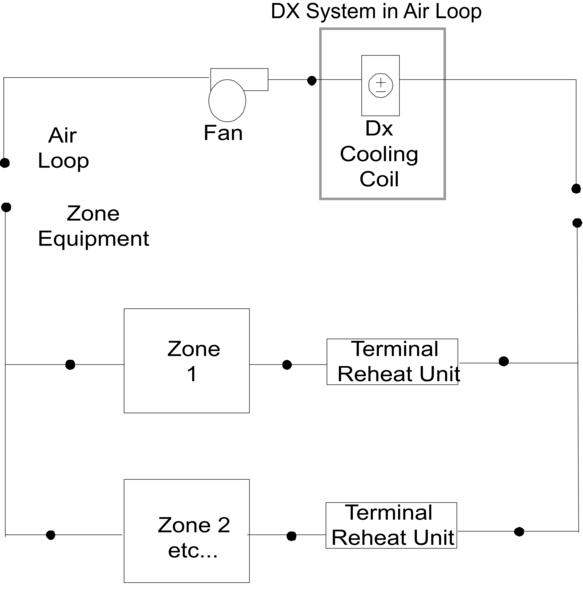
\includegraphics[width=0.9\textwidth, height=0.9\textheight, keepaspectratio=true]{media/image368.png}
\caption{Schematic of CoilSystem:Cooling:DX Object in an Air Loop for a Blow Through Application \protect \label{fig:schematic-of-coilsystem-cooling-dx-object-in}}
\end{figure}

\subsubsection{Inputs}\label{inputs-23-000}

\paragraph{Field: Name}\label{field-name-22-000}

This alpha field contains the identifying name for this component.

\paragraph{Field: Availability Schedule Name}\label{field-availability-schedule-name-13-000}

This alpha field contains the schedule name that contains information on the availability of the DX coil to operate. A schedule value of 0 indicates that the coil is off for that time period. A schedule value greater than 0 indicates that the coil can operate during the time period. If this field is blank, the schedule has values of 1 for all time periods.

\paragraph{Field: DX Cooling Coil System Inlet Node Name}\label{field-dx-cooling-coil-system-inlet-node-name}

This alpha field contains the identifying name given to the DX cooling coil inlet node, as specified in the DX cooling coil object.

\paragraph{Field: DX Cooling Coil System Outlet Node Name}\label{field-dx-cooling-coil-system-outlet-node-name}

This alpha field contains the identifying name given to the DX cooling coil outlet node, as specified in the cooling coil object.

\paragraph{Field: DX Cooling Coil System Sensor Node Name}\label{field-dx-cooling-coil-system-sensor-node-name}

This alpha field contains the identifying name given to the DX cooling coil control node, this is the node at which the temperature set point is specified by the set point manager.

\paragraph{Field: Cooling Coil Object Type}\label{field-cooling-coil-object-type-000}

This alpha field specifies the type of DX cooling coil. The valid choices for this field are:

\begin{itemize}
\item
  \hyperref[coilcoolingdxsinglespeed]{Coil:Cooling:DX:SingleSpeed}
\item
  \hyperref[coilsystemcoolingdxheatexchangerassisted]{CoilSystem:Cooling:DX:HeatExchangerAssisted}
\item
  \hyperref[coilcoolingdxtwospeed]{Coil:Cooling:DX:TwoSpeed}
\item
  \hyperref[coilcoolingdxtwostagewithhumiditycontrolmode]{Coil:Cooling:DX:TwoStageWithHumidityControlMode}
\item
  \hyperref[coilcoolingdxvariablespeed]{Coil:Cooling:DX:VariableSpeed}
\item
  \hyperref[coilcoolingdxsinglespeedthermalstorage]{Coil:Cooling:DX:SingleSpeed:ThermalStorage}
\end{itemize}

\paragraph{Field: Cooling Coil Name}\label{field-cooling-coil-name-000}

This alpha field contains the identifying name of the DX cooling coil.

As shown in the example below, correct specification of this system requires specification of the DX Cooling Coil object in addition to the CoilSystem:Cooling:DX object.

\paragraph{Field: Dehumidification Control Type}\label{field-dehumidification-control-type}

This alpha field contains the type of dehumidification control. The following options are valid for this field:

\textbf{None} - meet sensible load only, no active dehumidification control

\textbf{MultiMode} - activate enhanced dehumidification mode as needed and operate to meet the sensible load. If a sensible load exists, the system will operate to meet that sensible load and may not meet the latent load. If no sensible load exists, and Run on Latent Load = Yes, the system will operate to meet the entire latent load. This option is used to model DX equipment with a switchable option such as subcool reheat. It is valid only with Cooling coil type = \hyperref[coilcoolingdxtwostagewithhumiditycontrolmode]{Coil:Cooling:DX:TwoStageWithHumidityControlMode} or \hyperref[coilsystemcoolingdxheatexchangerassisted]{CoilSystem:Cooling:DX:HeatExchangerAssisted}. If the Run on Latent Load option below is set to Yes, this option may require the use of a heating coil and heating coil outlet air temperature set point manager downstream of this cooling coil to maintain the temperature set point.

\textbf{CoolReheat} - cool beyond the dry-bulb setpoint as required to meet the humidity setpoint. It is valid only with Cooling coil type = \hyperref[coilcoolingdxtwostagewithhumiditycontrolmode]{Coil:Cooling:DX:TwoStageWithHumidityControlMode}. This option requires the use of a heating coil and heating coil outlet air temperature set point manager downstream of this cooling coil to maintain the temperature set point.

The default is \textbf{None}. For all dehumidification controls, the max humidity setpoint on the control node is used. This must be set using a \textbf{\hyperref[zonecontrolhumidistat]{ZoneControl:Humidistat}} \textbf{\hyperref[zonecontrolhumidistat]{ZoneControl:Humidistat}} and one of:

\begin{itemize}
\item
  \textbf{\hyperref[setpointmanagersinglezonehumiditymaximum]{SetpointManager:SingleZone:Humidity:Maximum}}
\item
  \textbf{\hyperref[setpointmanagermultizonehumiditymaximum]{SetpointManager:MultiZone:Humidity:Maximum}}
\item
  \textbf{\hyperref[setpointmanagermultizonemaximumhumidityaverage]{SetpointManager:MultiZone:MaximumHumidity:Average}}
\end{itemize}

objects and \textbf{\hyperref[setpointmanageroutdoorairpretreat]{SetpointManager:OutdoorAirPretreat}} (optional) objects. When extra dehumidification is required, the equipment may not be able to meet the humidity setpoint if its full capacity is not adequate.

\paragraph{Field: Run on Sensible Load}\label{field-run-on-sensible-load}

This alpha field specifies if the unit will operate to meet a sensible load as determined by the inlet node dry-bulb temperature and the dry-bulb temperature setpoint on the control node. There are two valid choices, \textbf{Yes} or \textbf{No}. If \textbf{Yes}, unit will run if there is a sensible load. If \textbf{No}, unit will not run if there is only a sensible load. The default is \textbf{Yes}.

\paragraph{Field: Run on Latent Load}\label{field-run-on-latent-load}

This alpha field specifies if the unit will operate to meet a latent load as determined by the inlet node humidity ratio and the max humidity setpoint on the control node. There are two valid choices, \textbf{Yes} or \textbf{No}. If \textbf{Yes}, unit will run if there is a latent load. If both a sensible and latent load exist, the system will operate to maintain the temperature set point. When only a latent load exists, the system will operate to meet the humidity ratio set point and requires the use of a heating coil and heating coil outlet air temperature set point manager downstream of this cooling coil to maintain the temperature set point. If \textbf{No}, unit will not run if there is only a latent load. The default is \textbf{No}.

\paragraph{Field: Use Outdoor Air DX Cooling Coil}\label{field-use-outdoor-air-dx-cooling-coil}

This input field enables the Coil System DX Coil to be used for low air flow to capacity ratio range ( 100 300 cfm/ton). This flow to capacity ratio range is common in 100\% dedicated outdoor air system (DOAS) applications. Other airloop or zone HVAC systems may use this input filed if they operate at such a low flow to capacity ratio range. There are two valid choices, \textbf{Yes} or \textbf{No}. If \textbf{Yes}, the DX cooling coil is forced to operate in this flow to capacity ratio range or runs as 100\% DOAS DX coil. If \textbf{No}, DX coil is used as regular DX coil. This input field is optional.

\paragraph{Field: Outdoor Air DX Cooling Coil Leaving Minimum Air Temperature}\label{field-outdoor-air-dx-cooling-coil-leaving-minimum-air-temperature}

This input field is the DX cooling coil leaving supply air minimum temperature specified for frost control. The DX cooling coil leaving air temperature is not allowed to exceed this minimum coil leaving air temperature. The DX cooling coil frost controller adjusts or limits the desired coil outlet air setpoint temperature when the coil outlet temperature exceeds this minimum temperature limit specified. This input field is optional and only used along with in the input field above. The minimum and maximum values of this input field are 0.0 °C and 7.2 °C, and the default value is 2.0 °C.

An example IDF specification:

\begin{lstlisting}

CoilSystem:Cooling:DX,
  DX Cooling Coil System 1,!- Name
  CoolingCoilAvailSched,     !- Availability Schedule Name
  Cooling Coil Air Inlet Node,   !- DX Cooling Coil System Inlet Node Name
  Air Loop Outlet Node,       !- DX Cooling Coil System Outlet Node Name
  Air Loop Outlet Node,       !- DX Cooling Coil System Sensor Node Name
  Coil:Cooling:DX:SingleSpeed,   !- Cooling Coil Object Type
  ACDXCoil 1,                           !- Cooling Coil Name
  None,                                       !- Dehumidification Control Type
  Yes,                                         !- Run on Sensible Load
  No,                                           !- Run on Latent Load
  Yes,                                         !- Use DOAS DX Cooling Coil
  2.0;                                         !- DOAS DX Cooling Coil Leaving Minimum Air Temperature


  Coil:Cooling:DX:SingleSpeed,
  ACDXCoil 1,                           !- Name
  CoolingCoilAvailSched,     !- Availability Schedule Name
  25000,                                     !- Gross Rated Total Cooling Capacity {W}
  0.75,                                       !- Gross Rated Sensible Heat Ratio
  3.0,                                         !- Gross Rated Cooling COP
  1.3,                                         !- Rated Air Flow Rate {m3/s}
  Cooling Coil Air Inlet Node,   !- Air Inlet Node Name
  Air Loop Outlet Node,       !- Air Outlet Node Name
  WindACCoolCapFT,                 !- Total Cooling Capacity Function of Temperature Curve Name
  WindACCoolCapFFF,               !- Total Cooling Capacity Function of Flow Fraction Curve Name
  WindACEIRFT,                         !- Energy Input Ratio Function of Temperature Curve Name
  WindACEIRFFF,                       !- Energy Input Ratio Function of Flow Fraction Curve Name
  WindACPLFFPLR;                     !- Part Load Fraction Correlation Curve Name
\end{lstlisting}

\subsubsection{Outputs}\label{outputs-19}

\textbf{\emph{All DX Coils:}}

\begin{itemize}
\tightlist
\item
  HVAC,Average,Coil System Frost Control Status
\end{itemize}

\textbf{\emph{Coil Type = Coil:Cooling:DX:TwoStageWithHumidityControlMode \& Coil:Cooling:DX:VariableSpeed}}

\begin{itemize}
\item
  HVAC,Average,Coil System Cycling Ratio
\item
  HVAC,Average,Coil System Compressor Speed Ratio
\end{itemize}

\textbf{\emph{Coil:Cooling:DX:VariableSpeed}}

\begin{itemize}
\item
  HVAC,Average,Coil System Compressor Speed Number
\end{itemize}

\textbf{\emph{Coil types = Coil:Cooling:DX:SingleSpeed \& CoilSystem:Cooling:DX:HeatExchangerAssisted}}

\begin{itemize}
\tightlist
\item
  HVAC,Average,Coil System Part Load Ratio
\end{itemize}

\paragraph{Coil System Cycling Ratio}\label{coil-system-cycling-ratio}

The system may operate for the entire system timestep, but to meet the load the compressor can cycle on and off. This reports the fraction of the system timestep that the compressor is operating. (1.0 is continuous, 0.0 is off). For Coil:Cooling:VariableSpeed this description is true when compressor speed = 1. At higher compressor speeds Coil System Cycling Ratio = 1.

\paragraph{Coil System Compressor Speed Ratio}

This is the ratio of time in a system timestep that the compressor is at rated speed. The compressor speed ratio reports (1.0 is max, 0.0 is min) and any value in between as it is averaged over the timestep. This report is a duplicate of the report in Coil:Cooling:DX:VaraibleSpeed named Cooling Coil Neighboring Speed Levels Ratio.

\paragraph{Coil System Compressor Speed Number}\label{coil-system-compressor-speed-ratio}

This is the stage number that the compressor is operating at in a system timestep. The compressor speed number (from 1 to number of speeds) is reported and averaged over the timestep. This report is a duplicate of the report in Coil:Cooling:DX:VaraibleSpeed named Cooling Coil Upper Speed Level.

\paragraph{Coil System Part Load Ratio}\label{coil-system-part-load-ratio}

The DX system can operate with a cycling compressor or a varying speed compressor. This variable reports the fraction of the Full Load that is met during the system timestep. This can differ from the cycling part load ratio or the compressor speed ratio. (1.0 is Full Load and 0.0 is no load)

\paragraph{Coil System Frost Control Status}\label{coil-system-frost-control-status}

This is a flag indicating whether frost control is active at current time step or not. Frost control is activated or enforced when the sensible load control requires DX cooling coil outlet air temperature below the user specified minimum temperature or when the dehumidification load control requires DX cooling coil outlet air humidity ratio below the saturation humidity ratio corresponding to the user specified minimum temperature for frost control. Frost control status of zero means no active frost control, a value of 1 or 2 indicates that frost control is active. If frost control status is 1, then the frost control was enforced when the cooling coil is run to meet sensible load. If the frost control status value is 2, then the control was enforced when the cooling coil is run to meet latent load. When frost control is active the DX cooling coil setpoint value is modified based on user specified limit.

\subsection{CoilSystem:Heating:DX}\label{coilsystemheatingdx}

The CoilSystem:Heating:DX object is a virtual container component for a DX heating coil that provides the controls needed to operate the coil. Only single speed DX air-to-air heating coils are supported.

This component may be used as a heating coil in constant volume or variable volume air handlers. It can also be used in an outside air system (by including it in an \hyperref[airloophvacoutdoorairsystemequipmentlist]{AirLoopHVAC:OutdoorAirSystem:EquipmentList} object)or in a zone outdoor air unit (by including it in an \hyperref[zonehvacoutdoorairunitequipmentlist]{ZoneHVAC:OutdoorAirUnit:EquipmentList} object). This object is the one that is listed in the Branch or equipment list object rather than the coil itself.

The inlet and outlet nodes for the DX heat pump system are defined in the heating coil object. The control node is always the outlet node of the coil. This DX heat pump heating system requires that a (drybulb) temperature setpoint be placed on the outlet node using either a setpoint manager or the energy management system. The coil is controlled to attempt to meet that setpoint using a part load ratio modeling approach.

This model only supports continuous fan and cycling compressor operation -- cycling fan modeling is not available with this model.

\subsubsection{Inputs}\label{inputs-24}

\paragraph{Field: Name}\label{field-name-23-000}

This alpha field contains the identifying name for this component.

\paragraph{Field: Availability Schedule Name}\label{field-availability-schedule-name-14}

This alpha field contains the schedule name that contains information on the availability of the DX coil to operate. A schedule value of 0 indicates that the coil is off for that time period. A schedule value greater than 0 indicates that the coil can operate during the time period. If this field is blank, the schedule has values of 1 for all time periods.

\paragraph{Field: Heating Coil Object Type}\label{field-heating-coil-object-type-000}

This alpha field specifies the type of DX heating coil. This model currently supports only single speed DX heat pump heating coils and the only options for this field are \hyperref[coilheatingdxsinglespeed]{Coil:Heating:DX:SingleSpeed} and \hyperref[coilheatingdxvariablespeed]{Coil:Heating:DX:VariableSpeed}.

\paragraph{Field: Heating Coil Name}\label{field-heating-coil-name-000}

This alpha field specifies the unique name of the DX heating coil. This field references the name of a \hyperref[coilheatingdxsinglespeed]{Coil:Heating:DX:SingleSpeed} that needs to be defined elsewhere in the input file.

An example of a DX heating coil system follows.

\begin{lstlisting}

CoilSystem:Heating:DX,
  HeatPump DX Coil 1, !- Name
  FanAndCoilAvailSched , !- Availability Schedule Name
  Coil:Heating:DX:SingleSpeed,   !- Heating Coil Object Type
  Heat Pump DX Heating Coil 1;   !- Heating Coil Name


  Coil:Heating:DX:SingleSpeed,
  Heat Pump DX Heating Coil 1,   !- Name
  FanAndCoilAvailSched,       !- Availability Schedule Name
  autosize,                               !- Gross Rated Heating Capacity {W}
  2.75,                                       !- Gross Rated Heating COP {W/W}
  autosize,                               !- Rated Air Flow Rate {m3/s}
  Heating Coil Air Inlet Node,   !- Air Inlet Node Name
  SuppHeating Coil Air Inlet Node,   !- Air Outlet Node Name
  HPACHeatCapFT,                     !- Heating Capacity Function of Temperature Curve Name
  HPACHeatCapFFF,                   !- Heating Capacity Function of Flow Fraction Curve Name
  HPACHeatEIRFT,                     !- Energy Input Ratio Function of Temperature Curve Name
  HPACHeatEIRFFF,                   !- Energy Input Ratio Function of Flow Fraction Curve Name
  HPACCOOLPLFFPLR,                 !- Part Load Fraction Correlation Curve Name
  ,                                               !- Defrost Energy Input Ratio Function of Temperature Curve Name
  -8.0,                                       !- Minimum Outdoor Dry-Bulb Temperature for Compressor Operation {C}
  5.0,                                         !- Maximum Outdoor Dry-Bulb Temperature for Defrost Operation {C}
  200.0,                                     !- Crankcase Heater Capacity {W}
  10.0,                                       !- Maximum Outdoor Dry-Bulb Temperature for Crankcase Heater Operation {C}
  Resistive,                             !- Defrost Strategy
  TIMED,                                     !- Defrost Control
  0.166667,                               !- Defrost Time Period Fraction
  autosize,                               !- Resistive Defrost Heater Capacity {W}
  Heat Pump 1 Evaporator Node;
\end{lstlisting}

\subsubsection{Outputs}\label{outputs-20}

\paragraph{Coil System Part Load Ratio}\label{coil-system-part-load-ratio-1}

The DX system can operate with a cycling compressor or a varying speed compressor, This variable reports the fraction of the Full Load that is met during the system timestep. This can differ from the cycling part load ratio or the compressor speed ratio. (1.0 is Full Load and 0.0 is no load)

\subsection{CoilSystem:Cooling:DX:HeatExchangerAssisted}\label{coilsystemcoolingdxheatexchangerassisted}

The heat exchanger-assisted DX cooling coil is a virtual component consisting of a direct expansion (DX) cooling coil and an air-to-air heat exchanger as shown in Figure~\ref{fig:schematic-of-the-coilsystem-cooling-dx} below. The air-to-air heat exchanger pre-conditions the air entering the cooling coil, and reuses this energy to post-condition the supply air leaving the cooling coil. This heat exchange process improves the latent removal performance of the cooling coil by allowing it to dedicate more of its cooling capacity toward dehumidification (lower sensible heat ratio).

This compound object models the basic operation of an air-to-air heat exchanger in conjunction with a cooling coil. The heat exchanger-assisted DX cooling coil does not have an operating schedule of its own; its operating schedule is governed by the availability schedules for the DX cooling coil and the air-to-air heat exchanger. This compound object is used in the same way as a DX cooling coil object. It cannot be used directly on a branch. It must be contained within a parent object such as CoilSystem:Cooling:DX or AirloopHVAC:UnitarySystem and others which list CoilSystem:Cooling:DX:HeatExchangerAssisted as a valid cooling coil option.

To model a heat exchanger-assisted DX cooling coil, the input data file should include the following objects:

\begin{itemize}
\item
  CoilSystem:Cooling:DX:HeatExchangerAssisted object
\item
  Air-to-air heat exchanger object such as:
\begin{itemize}
\item
\hyperref[heatexchangerairtoairflatplate]{HeatExchanger:AirToAir:FlatPlate}
\item
\hyperref[heatexchangerairtoairsensibleandlatent]{HeatExchanger:AirToAir:SensibleAndLatent}
\item
\hyperref[heatexchangerdesiccantbalancedflow]{HeatExchanger:Desiccant:BalancedFlow}
\end{itemize}
\item
  DX cooling coil object (\hyperref[coilcoolingdxsinglespeed]{Coil:Cooling:DX:SingleSpeed} or \hyperref[coilcoolingdxvariablespeed]{Coil:Cooling:DX:VariableSpeed})
\end{itemize}

In terms of controlling the operation of the heat exchanger, the heat exchanger is assumed to always provide its heat transfer when the associated DX cooling coil is operating and no high humidity control mechanism is specified. However, the heat exchanger\textquotesingle s energy transfer may be controlled (i.e., turned on and off) based on a zone air humidity level using either a humidistat (ref. \hyperref[airloophvacunitarysystem]{AirLoopHVAC:UnitarySystem}, \hyperref[airloophvacunitaryfurnaceheatcool]{AirLoopHVAC:Unitary:Furnace:HeatCool} or \hyperref[airloophvacunitaryheatcool]{AirLoopHVAC:UnitaryHeatCool}) or a humidistat and a maximum humidity set point manager to place a humidity ratio set point on the appropriate control node (ref. \hyperref[coilsystemcoolingdx]{CoilSystem:Cooling:DX}). This model may also be used with the unitary changeover bypass system and the unitary air-to-air heat pump system (ref. \hyperref[airloophvacunitaryheatcoolvavchangeoverbypass]{AirLoopHVAC:UnitaryHeatCool:VAVChangeoverBypass} and \hyperref[airloophvacunitaryheatpumpairtoair]{AirLoopHVAC:UnitaryHeatPump:AirToAir}); however, the heat exchanger is assumed to always provide its heat transfer when the cooling coil operates and cannot be turned on and off based on a zone air humidity set point. Two zone air conditioners may also use this model for improved dehumidification. The first type is the packaged terminal heat pump (ref. \hyperref[zonehvacpackagedterminalheatpump]{ZoneHVAC:PackagedTerminalHeatPump}) where the heat exchanger's heat transfer is always active whenever the cooling coil operates. The second type is the window air conditioner (ref. \hyperref[zonehvacwindowairconditioner]{ZoneHVAC:WindowAirConditioner}) where the heat exchanger's heat transfer is always active when the cooling coil operates and no high humidity control mechanism is specified, OR the heat exchanger's heat transfer may be controlled based on zone air humidity level if a humidistat and high humidity set point manager are specified (maximum humidity ratio set point placed on the heat exchanger's exhaust air outlet node, ref. Figure~\ref{fig:schematic-of-the-coilsystem-cooling-dx}).

Links to the cooling coil and air-to-air heat exchanger specifications are provided in the input data syntax for this compound object. A description of each input field for this compound object is provided below.

\begin{figure}[hbtp] % fig 139
\centering
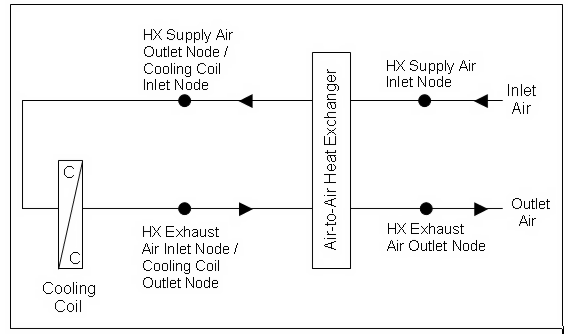
\includegraphics[width=0.9\textwidth, height=0.9\textheight, keepaspectratio=true]{media/image369.png}
\caption{Schematic of the CoilSystem:Cooling:DX:HeatExchangerAssisted compound object \protect \label{fig:schematic-of-the-coilsystem-cooling-dx}}
\end{figure}

NOTE: Node naming shown in Figure~\ref{fig:schematic-of-the-coilsystem-cooling-dx} is representative for \hyperref[heatexchangerairtoairsensibleandlatent]{HeatExchanger:AirToAir:SensibleAndLatent}. For \hyperref[heatexchangerairtoairflatplate]{HeatExchanger:AirToAir:FlatPlate}, the exhaust air nodes are referred to as secondary air nodes. For \hyperref[heatexchangerdesiccantbalancedflow]{HeatExchanger:Desiccant:BalancedFlow}, the supply air nodes are referred to as regeneration air nodes and the exhaust air nodes as process air nodes.

\subsubsection{Inputs}\label{inputs-25}

\paragraph{Field: Name}\label{field-name-24-000}

A unique user-assigned name for the heat exchanger-assisted DX cooling coil. Any reference to this compound component by another object will use this name.

\paragraph{Field: Heat Exchanger Object Type}\label{field-heat-exchanger-object-type-000}

This alpha field denotes the type of heat exchanger being modeled. Valid choices are:

\begin{itemize}
\item
  \hyperref[heatexchangerairtoairflatplate]{HeatExchanger:AirToAir:FlatPlate}
\item
  \hyperref[heatexchangerairtoairsensibleandlatent]{HeatExchanger:AirToAir:SensibleAndLatent}
\item
  \hyperref[heatexchangerdesiccantbalancedflow]{HeatExchanger:Desiccant:BalancedFlow}
\end{itemize}

\paragraph{Field: Heat Exchanger Name}\label{field-heat-exchanger-name-001}

This alpha field denotes the name of the air-to-air heat exchanger being modeled.

\paragraph{Field: Cooling Coil Object Type}\label{field-cooling-coil-object-type-1}

This alpha field denotes the type of DX cooling coil being modeled. The only valid choices are \hyperref[coilcoolingdxsinglespeed]{Coil:Cooling:DX:SingleSpeed} or \hyperref[coilcoolingdxvariablespeed]{Coil:Cooling:DX:VariableSpeed}.

\paragraph{Field: Cooling Coil Name}\label{field-cooling-coil-name-1}

This alpha field denotes the name of the DX cooling coil being modeled.

Following is an example input for this compound object:

\begin{lstlisting}

CoilSystem:Cooling:DX:HeatExchangerAssisted,
  HeatExchangerAssistedCoolingCoil,               ! Name of the heat exchanger assisted cooling coil
  HeatExchanger:AirToAir:SensibleAndLatent,       ! Heat exchanger type
  Air to Air Heat Exchanger 1,                    ! Heat exchanger name
  Coil:Cooling:DX:SingleSpeed,                    ! Cooling coil type
  DX Cooling Coil 1;                              ! Cooling coil name


  HeatExchanger:AirToAir:SensibleAndLatent,
  Air to Air Heat Exchanger 1,        !- Heat exchanger name
  FanAndCoilAvailSched,               !- Availability schedule name
  1.3,                                !- Nominal supply air flow rate {m3/s}
  .2,                                 !- Sensible effectiveness at 100% airflow heating condition
  .0,                                 !- Latent effectiveness at 100% airflow heating condition
  .23,                                !- Sensible effectiveness at 75% airflow heating condition
  .0,                                 !- Latent effectiveness at 75% airflow heating condition
  .2,                                 !- Sensible effectiveness at 100% airflow cooling condition
  .0,                                 !- Latent effectiveness at 100% airflow cooling condition
  .23,                                !- Sensible effectiveness at 75% airflow cooling condition
  .0,                                 !- Latent effectiveness at 75% airflow cooling condition
  HeatExchangerSupplyAirInletNode,    !- Supply air inlet node name
  DX Cooling Coil Air Inlet Node,     !- Supply air outlet node name
  HeatExchangerExhaustAirInletNode,   !- Exhaust air inlet node name
  HeatExchangerExhaustAirOutletNode,  !- Exhaust air outlet node name
  50.0,                               !- Nominal electric power {W}
  No,                                 !- Supply air outlet temperature control
  Rotary,                             !- Heat exchanger type
  None;                               !- Frost control type


  Coil:Cooling:DX:SingleSpeed,
  DX Cooling Coil 1,                  !- Coil Name
  FanAndCoilAvailSched,               !- Availability Schedule
  25000,                              !- Gross Rated Total Cooling Capacity {W}
  0.75,                               !- Gross Rated Sensible Heat Ratio
  3.0,                                !- Gross Rated Cooling COP
  1.3,                                !- Rated Air Flow Rate {m3/s}
  DX Cooling Coil Air Inlet Node,     !- Coil Air Inlet Node
  HeatExchangerExhaustAirInletNode,   !- Coil Air Outlet Node
  ACCoolCapFT,                  !- Total Cooling Capacity Modifier Curve (function of temperature)
  ACCoolCapFFF,                 !- Total Cooling Capacity Modifier Curve (function of flow fraction)
  ACEIRFT,                      !- Energy Input Ratio Modifier Curve (function of temperature)
  ACEIRFFF,                     !- Energy Input Ratio Modifier Curve (function of flow fraction)
  ACPLFFPLR;                    !- Part Load Fraction Correlation (function of part load ratio)
\end{lstlisting}

\subsubsection{Outputs}\label{outputs-21}

No variables are reported for this compound object. However, outputs are provided by the cooling coil and heat exchanger that are specified.

\subsection{CoilSystem:IntegratedHeatPump:AirSource}\label{ASIHPIO}

CoilSystem:IntegratedHeatPump:AirSource is a collection of all the working modes in an air-source integrated heat pump, including space cooling (SC), space heating (SH), dedicated water heating (DWH), combined space cooling and water heating with full condensing(SCWH), combined space cooling and water heating with desuperheating (SCDWH), combined space heating and water heating with desuperheating (SHDWH). These working modes should also be referred to in other related air loop or water loop parent objects, for example, \hyperref[airloophvacunitarysystem]{AirLoopHVAC:UnitarySystem} and \hyperref[waterheaterheatpumppumpedcondenser]{WaterHeater:HeatPump:PumpedCondenser}, to represent the air side and water side node connections, and facilitate iterating the speed to match the space conditioning or water heating load. In addition, CoilSystem:IntegratedHeatPump:AirSource contains a series of criteria for selecting a working mode at the beginning of each timestep.

\subsubsection{Inputs}\label{inputs-ASIHP}

\paragraph{Field: Name}\label{field-name-ASIHP}

This alpha field defines a unique user-assigned name for an instance of an air-source integrated heat pump.

\paragraph{Field: Supply Water Monitoring Node Name}\label{Field-Supply-Water-Monitoring-Node-Name-ASIHP}

This alpha field defines a water side node to monitor the supply water amount after the water heating operation of the integrated heat pump is turned on.

\paragraph{Field: Space Cooling Mode Coil Name}\label{Field-Space-Cooling-Mode-Coil-Name-ASIHP}

This alpha field defines the space cooling (SC) mode in an ASIHP, which must be given. The SC mode refers to the name of a \hyperref[coilcoolingdxvariablespeed]{Coil:Cooling:DX:VariableSpeed} object, which contains all the performance curves and rated values to describe the space cooling operation.

\paragraph{Field: Space Heating Mode Coil Name}\label{Field-Space-Heating-Mode-Coil-Name-ASIHP}

This alpha field defines the space heating (SH) mode in the ASIHP, which must be given. The SH mode refers to the name of a \hyperref[coilheatingdxvariablespeed]{Coil:Heating:DX:VariableSpeed} object, which contains all the performance curves and rated values to describe the space heating operation.

\paragraph{Field: Water Heating Mode Coil Name}\label{Field-Water-Heating-Mode-Coil-Name-ASIHP}

This alpha field defines the dedicated water heating (DWH) mode in the ASIHP, which must be given. The DWH mode refers to the name of a Coil:WaterHeating:AirToWaterHeatPump:--VariableSpeed object, which contains all the performance curves and rated values to describe the water heating operation with outdoor air source.

\paragraph{Field: SCWH Mode Coil Name}\label{Field-SCWH-Mode-Coil-Name-ASIHP}

This alpha field defines the combined space cooling and water heating with full condensing (SCWH) in an ASIHP, which must be given. The SCWH mode refers to the name of a Coil:WaterHeating:AirToWaterHeatPump:VariableSpeed object, which contains all the performance curves and rated values to describe the water heating operation with an indoor air source. The SCWH mode is connected to the same WaterHeater:HeatPump:PumpedCondenser as the DWH mode, and the same air side node connections as the SC mode.

\paragraph{Field: SCDWH Mode Cooling Coil Name}\label{Field-SCDWH-Mode-Cooling-Coil-Name-ASIHP}

This alpha field defines the cooling operation in the combined space cooling and water heating with desuperheating (SCDWH) mode in an ASIHP, which must be given. These should be a different object from the SC mode. It should be noted that the rated power and power correction curves are contained in the \hyperref[coilcoolingdxvariablespeed]{Coil:Cooling:DX:VariableSpeed} object. That means the power consumption at each speed level of the SCDWH mode is accounted for by the cooling coil part.

\paragraph{Field: SCDWH Mode Water Heating Coil Name}\label{Field-SCDWH-Mode-Water-Heating-Coil-Name-ASIHP}

This alpha field defines the water heating operation in the combined space cooling and water heating with desuperheating (SCDWH) mode in an ASIHP, which must be given. The power values and curves in the Coil:WaterHeating:AirToWaterHeatPump:VariableSpeed are not used. That means the power consumption at each speed level of the SCDWH mode is accounted for by the cooling coil part.

\paragraph{Field: SHDWH Mode Heating Coil Name}\label{Field-SHDWH-Mode-Heating-Coil-Name-ASIHP}

This alpha field defines the heating operation in the combined space heating and water heating with desuperheating (SHDWH) mode in an ASIHP, which must be given. This should be a different object from the SH mode. It should be noted that the rated power and power correction curves are contained in the \hyperref[coilheatingdxvariablespeed]{Coil:Heating:DX:VariableSpeed} object. That means the power consumption at each speed level of the SHDWH mode is accounted for by the cooling coil part.

\paragraph{Field: SHDWH Mode Water Heating Coil Name}\label{Field-SHDWH-Mode-Water-Heating-Coil-Name-ASIHP}

This alpha field defines the water heating operation in the combined space heating and water heating with desuperheating (SCDWH) mode in an ASIHP, which must be given. The power values and curves in the Coil:WaterHeating:AirToWaterHeatPump:VariableSpeed are not used. That means the power consumption at each speed level of the SHDWH mode is accounted for by the heating coil part.

\paragraph{Field: SCWH Mode Minimum Indoor Temperature to Allow  Overcooling}\label{Field-SCWH-Minimum-In-Overcooling-ASIHP}

This numeric field defines an indoor air temperature [C] above which indoor overcooling is allowed in the cooling operation, i.e., allowing running the SCWH mode to cool down the indoor air below the thermostat setting temperature, and iterate the compressor speed to match the water heating load. It has to be noted that both the indoor temperature and ambient temperature lower bound settings have to be satisfied when allowing indoor overcooling by running the SCWH mode.


\paragraph{Field: SCWH Mode Minimum Outdoor Temperature to Allow Overcooling}\label{Field-SCWH-Minimum-Outdoor-ASIHP}

This numeric field defines an ambient air temperature above which indoor overcooling is allowed in the cooling operation, i.e., allowing running the SCWH mode to cool down the indoor air below the thermostat setting temperature, and iterate the compressor speed to match the water heating load. It has to be noted that both the indoor temperature and ambient temperature lower bound settings have to be satisfied when allowing overcooling the indoor by running the SCWH mode.

\paragraph{Field: Minimum Indoor Temperature to Ignore Space Heating Call}\label{Field-Minimum-Indoor-IgnoreSH-ASIHP}

This numeric field defines an indoor air temperature [C] above which the water heating request has the higher priority and the space heating call can be ignored. The ASIHP will run the DWH mode to match the water heating load regardless of space heating call. It has to be noted that both the indoor temperature and ambient temperature lower bound settings have to be satisfied when a space heating call can be ignored.


\paragraph{Field: Minimum Outdoor Temperature to Ignore Space Heating Call}\label{Field-Minimum-Outdoor-IgnoreSH-ASIHP}

This numeric field defines an ambient air temperature [C] above which the water heating request has the higher priority and the space heating call can be ignored. The ASIHP will run the DWH mode to match the water heating load regardless of space heating call. It has to be noted that both the indoor temperature and ambient temperature lower bound settings have to be satisfied when a space heating call can be ignored.


\paragraph{Field: SCWH Mode Load Matching Type}\label{Field-SCWH-Matching-Type-ASIHP}

This choice field specifies the control in the SCWH mode. The choices are CoolingLoad or WaterHeatingLoad. During the SCWH operation when both the space cooling and water heating calls exist, if the field is CoolingLoad, it means that the compressor speed is iterated to match the space cooling load, and the water heating energy is a byproduct.  If this field is WaterHeatingLoad, it means that the speed is altered to match the water heating load, and the space cooling energy is a byproduct.



\paragraph{Field: SCWH Mode Minimum Speed}\label{Field-SCWH-Minimum-Speed-ASIHP}

This numeric field defines a minimum speed level for running the SCWH; i.e., the compressor speed will be altered between the minimum speed specified and top speed, responding to the simultaneous space cooling and water heating calls. If there is only a water heating call, this input will not be used.

\paragraph{Field: SCDWH Mode Maximum Heated Water Vol Before Switching to SCWH}\label{Field-SCDWH-Max-Water-ASIHP}

This numeric field defines an accumulative, heated water volume [m3] before switching from SCDWH to SCWH mode. When there are simultaneous space cooling and water heating calls, the ASIHP will run SCDWH first to satisfy a small water heating load. If the water volume heated by the heat pump goes beyond the limit, it means that the SCDWH, which uses a desuperheater, cannot provide enough capacity for the water heating request, and thus the SCWH mode will be turned on.



\paragraph{Field: SCDWH Mode Minimum Speed}\label{Field-SCDWH-MinSped-ASIHP}

This numeric field defines a minimum speed level for running the SCDWH; i.e., the compressor speed will be altered between the minimum speed specified and top speed to match the space cooling load, and the water heating energy is a byproduct.

\paragraph{Field: SHDWH Mode Time Limit Before Turning on Electric Water Heating Element}\label{Field-SHDWH-HeatElemement-ASIHP}

This numeric field defines the running time [s] of the SHDWH mode before electric heating elements in the connected water tank are turned on if the water heating request cannot be satisfied on time. When there are simultaneous space heating and water heating calls, the ASIHP will run SHDWH mode first to satisfy a small water heating load. If the running time goes beyond the time limit, it means that the SHDWH mode, which uses a desuperheater, cannot provide enough capacity for the water heating request, and thus the electric elements in the water tank will be turned on to supplement the heating capacity.

\paragraph{Field: SHDWH Mode Minimum Speed}\label{Field-SHDWH-Mode-Minimum-Speed-ASIHP}

This numeric field defines a minimum speed level for running the SHDWH mode; i.e., the compressor speed will be altered between the minimum speed and top speed to match the space heating load. Consequently, the water heating capacity is the byproduct.



\paragraph{An IDF example:}\label{FieldIDFExample-ASIHP}


An IDF example showing how this object is:


\begin{lstlisting}
CoilSystem:IntegratedHeatPump:AirSource,
  ASIHP1,        !- Name of an air-source integrated heat pump
  TankoutNod,    !- Name of a water node for  monitoring the supply water flow amount
  SCCoil1,       !- Coil object Name of space cooling mode
  SHCoil1,       !- Coil object Name of space heating mode
  DWHCoil1,      !- Coil object Name of dedicated water heating mode
  SCWHCoil1,     !- Coil object Name for SCWH mode
  SCDWHCoil1     !- Coil object Name for cooling part of SCDWH mode
  SCDWHCoil2     !- Coil object Name for WH part of SCDWH mode
  SHDWHCoil1     !- Coil object Name for space heating part of SHDWH mode
  SHDWHCoil2     !- Coil object Name for WH part of SHDWH mode
  23.0,          !-{C},indoor temperature above which indoor overcooling is allowed
  28.0,          !-{C},outdoor temperature above which indoor overcooling is allowed
  20.0,          !-{C},indoor temperature above which water heating has the higher priority
  16.0,          !-{C},outdoor temperature above which water heating has the higher priority
  0,             !-0: match cooling load, 1: match water heating load in SCWH mode
  2,             !- minimum speed level for SCWH mode
  3.0,           !- {m3}, limit of heated water volume before switching from SCDWH to SCWH mode
  2,             !- minimum speed level for SCDWH mode
  600,           !- {s}, time limit before turning on electric element in SHDWH mode
  5;             !- minimum speed level for SHDWH mode
\end{lstlisting}

\subsubsection{Outputs}\label{outputs-011}

The output variables that are available for this air source integrated heat pump are shown below:

\begin{itemize}
\item
  HVAC, Average, Integrated Heat Pump Air Loop Mass Flow Rate {[}kg/s{]}
\item
  HVAC, Average, Integrated Heat Pump Condenser Water Mass Flow Rate {[}kg/s{]}
\item
  HVAC, Average, Integrated Heat Pump Air Total Cooling Rate {[}W{]}
\item
  HVAC, Average, Integrated Heat Pump Air Heating Rate {[}W{]}
\item
  HVAC, Average, Integrated Heat Pump Water Heating Rate {[}W{]}
\item
  HVAC, Average, Integrated Heat Pump Electricity Rate {[}W{]}
\item
  HVAC, Average, Integrated Heat Pump Air Latent Cooling Rate {[}W{]}
\item
  HVAC, Average, Integrated Heat Pump Source Heat Transfer Rate {[}W{]}
 \item
  HVAC, Average, Integrated Heat Pump COP {[}{]}
 \item
  HVAC, Sum, Integrated Heat Pump Electricity Energy {[}J{]}
 \item
  HVAC, Sum, Integrated Heat Pump Air Total Cooling Energy {[}J{]}
  \item
  HVAC, Sum, Integrated Heat Pump Air Heating Energy {[}J{]}
\item
  HVAC, Sum, Integrated Heat Pump Water Heating Energy {[}J{]}
 \item
  HVAC, Sum, Integrated Heat Pump Air Latent Cooling Energy {[}J{]}
 \item
  HVAC, Sum, Integrated Heat Pump Source Heat Transfer Energy {[}J{]}

\end{itemize}

\paragraph{Integrated Heat Pump Air Loop Mass Flow Rate {[}kg/s{]}}\label{Out-Air-Loop-Flow-Rate-ASIHP}
The output variable is the air mass flow rate in the indoor air loop, over the timestep being reported.

\paragraph{Integrated Heat Pump Condenser Water Mass Flow Rate {[}kg/s{]}}\label{Out-Cond-water-Flow-ASIHP}

The output variable is the hot water mass flow rate through the condenser of the heat pump water heater, over the timestep being reported.

\paragraph{Integrated Heat Pump Air Total Cooling Rate {[}W{]}}\label{Out-Cooling-Coil-Total-Cooling-Rate-ASIHP}

The output variable is the average total cooling load provided by the integrated heat pump, which includes the sensible and latent load in watts over the timestep being reported.


\paragraph{Integrated Heat Pump Air Heating Rate {[}W{]}}\label{Out-Heating-Total-Air-Heating-Rate-ASIHP}

The output variable is the average total heating load provided by the integrated heat pump in watts over the timestep being reported.


\paragraph{Integrated Heat Pump Water Heating Rate {[}W{]}}\label{Out-Total-Water-Heating-Rate-ASIHP}

The output variable is the average total water heating load provided by the integrated heat pump in watts over the timestep being reported.

\paragraph{Integrated Heat Pump Electricity Rate {[}W{]}}\label{Out-Total-Electric-Power-ASIHP}

The output variable is the average total electric power consumed by the integrated heat pump in watts over the timestep being reported.


\paragraph{Integrated Heat Pump Air Latent Cooling Rate {[}W{]}}\label{Out-Total-Latent-Cooling-Rate-ASIHP}

The output variable is the average latent cooling load provided by the integrated heat pump in watts over the timestep being reported.

\paragraph{Integrated Heat Pump Source Heat Transfer Rate {[}W{]}}\label{Out-Total-Source-Energy-Rate-ASIHP}

The output variable is the average total source energy rate absorbed or discharged to the outdoor air by the integrated heat pump in watts over the timestep being reported.


\paragraph{Integrated Heat Pump COP {[}{]}}\label{Out-Tot-COP-ASIHP}

The output variable is the average total COP (using the total delivered load divided by the electric power) by the integrated heat pump in watts over the timestep being reported. The total delivered load includes all the incurred space cooling, water heating, and space heating loads.


\paragraph{Integrated Heat Pump Electricity Energy {[}J{]}}\label{Out-Total-Electric-Energy-ASIHP}

The output variable is the electric consumption of the integrated heat pump in joules over the timestep being reported.


\paragraph{Integrated Heat Pump Air Total Cooling Energy {[}J{]}}\label{Out-Total-Cooling-Energy-ASIHP}
The output variable is the total space cooling output of the integrated heat pump in joules over the timestep being reported.


\paragraph{Integrated Heat Pump Air Heating Energy {[}J{]}}\label{Out-Total-Air-Heating-Energy-ASIHP}

The output variable is the total space heating output of the integrated heat pump in joules over the timestep being reported.

\paragraph{Integrated Heat Pump Water Heating Energy{[}J{]}}\label{Out-Total-WH-Energy-ASIHP}
The output variable is the total water heating output of the integrated heat pump in joules over the timestep being reported.


\paragraph{Integrated Heat Pump Air Latent Cooling Energy {[}J{]}}\label{Out-Total-LatCooling-Energy-ASIHP}
The output variable is the total latent cooling output of the integrated heat pump in joules over the timestep being reported.

\paragraph{Integrated Heat Pump Source Heat Transfer Energy {[}J{]}}\label{Out-Total-Source-Energy-ASIHP}
The output variable is the total source energy output of the integrated heat pump in joules, absorbed or discharged to the outdoor air, over the timestep being reported.

\subsection{Coil:WaterHeating:AirToWaterHeatPump:Pumped}\label{coilwaterheatingairtowaterheatpumppumped}

EnergyPlus can model a heat pump water heater (HPWH) consisting of a water heater tank (e.g., \lstinline!WaterHeater:Mixed!), a direct expansion (DX) coil (i.e., an air-to-water DX compression system which includes a water heating coil, air coil, compressor, and water pump), and a fan to provide air flow across the air coil associated with the DX compression system. These objects work together to model a system which heats water using zone air, outdoor air, or a combination of zone and outdoor air as the primary heat source. From the air-side heat transfer perspective, the water-heater receives heating energy from air. Thus it is considered as a cooling coil, and the output variable names are using "Cooling Coil".

The \hyperref[waterheaterheatpumppumpedcondenser]{\lstinline!WaterHeater:HeatPump:PumpedCondenser!} compound object, water heater tank object (e.g., \hyperref[waterheatermixed]{\lstinline!WaterHeater:Mixed!}), and fan object (e.g., \hyperref[fanonoff]{\lstinline!Fan:OnOff!}) are defined elsewhere in this reference document. \lstinline!Coil:WaterHeating:AirToWaterHeatPump:Pumped! object described here models an air-to-water DX compression system to determine its air-side and water-side performance. This DX coil object calculates the air-side sensible and latent cooling capacity at the specific operating conditions for each simulation timestep, as well as the condenser's water-side temperature difference at a given condenser water flow rate.

The heat pump water heater DX coil model performs the following major functions:

\begin{itemize}
\item
  calculates the electric consumption of the DX compressor and water pump
\item
  calculates the amount of heat delivered to the water tank
\item
  calculates the electric consumption of the compressor's crankcase heater
\item
  calculates the air-side performance of the DX coil
\end{itemize}

The input fields for this object are described below in detail:

\subsubsection{Inputs}\label{inputs-27}

\paragraph{Field: Name}\label{field-name-26-000}

This alpha field defines a unique user-assigned name for an instance of a heat pump water heater DX coil. Any reference to this coil by another object (e.g., \hyperref[waterheaterheatpumppumpedcondenser]{\lstinline!WaterHeater:HeatPump:PumpedCondenser!}) will use this name.

\paragraph{Field: Rated Heating Capacity}\label{field-rated-heating-capacity}

This numeric field defines the DX coil heating capacity in Watts at the rated evaporator inlet air temperatures, rated condenser inlet water temperature, rated evaporator air flow rate, and rated condenser water flow rate specified below. Values must be greater than 0. This value represents water heating capacity, and it may or may not include the impact of condenser pump heat (see field Condenser Pump Heat Included in Rated Heating Capacity below).

\paragraph{Field: Rated COP}\label{field-rated-cop}

This numeric field defines the DX coil's water heating coefficient of performance (COP = water heating capacity in watts divided by electrical power input in watts) at rated conditions (rated inlet temperatures and flow rates specified below). This input not only determines the electric energy use of the heat pump DX coil, but also the amount of total air cooling provided by the evaporator. The rated COP includes compressor power, and may or may not include condenser pump power or evaporator fan power (see field Evaporator Fan Power Included in Rated COP and field Condenser Pump Power Included in Rated COP). Values must be greater than 0. If this field is left blank, the default value is 3.2.

\paragraph{Field: Rated Sensible Heat Ratio}\label{field-rated-sensible-heat-ratio-1}

This numeric field defines the air-side sensible heat ratio (SHR = sensible cooling capacity divided by total cooling capacity) of the DX coil at rated conditions (rated inlet temperatures and flow rates specified below). This value should not include the effect of evaporator fan heat. Values must be greater than or equal to 0.5, and less than or equal to 1.0. The default value is 0.85.

\paragraph{Field: Rated Evaporator Inlet Air Dry-Bulb Temperature}\label{field-rated-evaporator-inlet-air-dry-bulb-temperature}

This numeric field defines the evaporator inlet air dry-bulb temperature, in degrees Celsius, that corresponds to rated coil performance (heating capacity, COP and SHR). Values must be greater than 5 °C. If this field is left blank, the default value is 19.7 °C.

\paragraph{Field: Rated Evaporator Inlet Air Wet-Bulb Temperature}\label{field-rated-evaporator-inlet-air-wet-bulb-temperature}

This numeric field defines the evaporator inlet air wet-bulb temperature, in degrees Celsius, that corresponds to rated coil performance (heating capacity, COP and SHR). Values must be greater than 5 °C. If this field is left blank, the default value is 13.5 °C.

\paragraph{Field: Rated Condenser Inlet Water Temperature}\label{field-rated-condenser-inlet-water-temperature}

This numeric field defines the condenser inlet water temperature, in degrees Celsius, that corresponds to rated coil performance (heating capacity, COP and SHR). Values must be greater than 25 °C. If this field is left blank, the default value is 57.5 °C.

\paragraph{Field: Rated Evaporator Air Flow Rate}\label{field-rated-evaporator-air-flow-rate}

This numeric field defines the evaporator air volume flow rate in cubic meters per second at rated conditions. Values must be greater than 0. If this field is left blank or autocalculated (field value = \textbf{autocalculate}), the default value is 5.035E-5 m\(^{3}\)/s/W (31.25 cfm/MBH) multiplied by the Rated Heating Capacity specified above. When autocalculating the rated evaporator air volumetric flow rate, a zone sizing object is not required.

\paragraph{Field: Rated Condenser Water Flow Rate}\label{field-rated-condenser-water-flow-rate}

This numeric field defines the condenser water volumetric flow rate in cubic meters per second at rated conditions. Values must be greater than 0. If this field is left blank or autocalculated (field value = \textbf{autocalculate}), the default value is 4.487E-8 m\(^{3}\)/s/W (0.208 gpm/MBH) multiplied by the Rated Heating Capacity specified above. When autocalculating the rated condenser water volumetric flow rate, a zone sizing object is not required. A warning message will be issued if the ratio of Rated Condenser Water Volumetric Flow Rate to Rated Heating Capacity is less than 1.79405E-8 m\(^{3}\)/s/W (0.083 gpm/MBH) or greater than 8.97024E-8 m\(^{3}\)/s/W (0.417 gpm/MBH), but the simulation will continue.

\paragraph{Field: Evaporator Fan Power Included in Rated COP}\label{field-evaporator-fan-power-included-in-rated-cop}

This choice field specifies if evaporator fan power is included in the rated COP defined above. This input impacts the calculation of compressor electric power and total air cooling provided by the evaporator for each simulation timestep. If Yes is selected, the evaporator fan power is subtracted from the total electric heating power when calculating total evaporator cooling capacity. If No is selected, it is assumed that the total heating power does not include evaporator fan power. If this field is left blank, the default is Yes. See the Engineering Reference section for \lstinline!Coil:WaterHeating:AirToWaterHeatPump:\*! for further details.

\paragraph{Field: Condenser Pump Power Included in Rated COP}\label{field-condenser-pump-power-included-in-rated-cop}

This choice field specifies if condenser pump power is included in the rated COP defined above. This input impacts the calculation of compressor electric power which then impacts the total air cooling provided by the evaporator for each simulation timestep. If Yes is selected, the condenser pump power is subtracted from the total electric heating power when calculating total evaporator cooling capacity. If No is selected, it is assumed that the total heating power does not include the condenser pump. If this field is left blank, the default is No. See Engineering Reference section for \lstinline!Coil:WaterHeating:AirToWaterHeatPump:\*! for further details.

\paragraph{Field: Condenser Pump Heat Included in Rated Heating Capacity and Rated COP}\label{field-condenser-pump-heat-included-in-rated-heating-capacity-and-rated-cop}

This choice field specifies if condenser pump heat is included in the rated heating capacity and rated COP defined above. This input impacts the calculation of compressor electric power and total air cooling provided by the evaporator for each simulation timestep. If Yes is selected, the condenser pump heat is already included in the rated heating capacity and rated COP. If No is selected, it is assumed that the rated heating capacity and rated COP do not include the condenser pump heat, and pump heat is added to the total water heating capacity based on the Condenser Water Pump Power and Fraction of Condenser Pump Heat to Water fields below. If this field is left blank, the default is No. See Engineering Reference section for \lstinline!Coil:WaterHeating:AirToWaterHeatPump:\*! for further details.

\paragraph{Field: Condenser Water Pump Power}\label{field-condenser-water-pump-power}

This numeric field defines the DX coil's condenser pump power in Watts. This is the operating pump power as installed. Values must be greater than or equal to 0. If this field is left blank, the default value is 0. A warning message will be issued if the ratio of Condenser Water Pump Power to Rated Heating Capacity exceeds 0.1422 W/W (41.67 Watts/MBH), but the simulation will continue.

\paragraph{Field: Fraction of Condenser Pump Heat to Water}\label{field-fraction-of-condenser-pump-heat-to-water}

This numeric field defines the fraction of condenser pump heat that is transferred to the condenser water. The pump is assumed to be downstream of the condenser water coil, and this field is used to determine the water temperature at the condenser outlet node when the field Condenser Pump Power Included in Rated Heating Capacity is set to No. Values must be greater than or equal to 0 and less than or equal to 1. If this field is left blank, the default value is 0.2.

\paragraph{Field: Evaporator Air Inlet Node Name}\label{field-evaporator-air-inlet-node-name-1}

This alpha field defines the name of the air node from which the evaporator coil draws its inlet air.

\paragraph{Field: Evaporator Air Outlet Node Name}\label{field-evaporator-air-outlet-node-name}

This alpha field defines the name of the air node to which the evaporator coil sends its outlet air.

\paragraph{Field: Condenser Water Inlet Node Name}\label{field-condenser-water-inlet-node-name}

This alpha field defines the name of the node from which the DX coil condenser draws its inlet water. This node name must also match the source side outlet node name for the water heater tank connected to this DX coil (ref: Water Heaters).

\paragraph{Field: Condenser Water Outlet Node Name}\label{field-condenser-water-outlet-node-name}

This alpha field defines the name of the node to which the heat pump condenser sends it outlet water. This node name must also match the source side inlet node name for the water heater tank connected to this DX coil (ref: Water Heaters).

\paragraph{Field: Crankcase Heater Capacity}\label{field-crankcase-heater-capacity-7}

This numeric field defines the compressor's crankcase heater capacity in Watts. The crankcase heater only operates when the compressor is off and the air surrounding the compressor is below the Maximum Ambient Temperature for Crankcase Heater Operation specified below.

\paragraph{Field: Maximum Ambient Temperature for Crankcase Heater Operation}\label{field-maximum-ambient-temperature-for-crankcase-heater-operation}

This numeric field defines the maximum ambient temperature for crankcase heater operation in degree Celsius. The crankcase heater only operates when the air surrounding the compressor is below this maximum temperature value and the compressor is off. The ambient temperature surrounding the compressor is set by the Heat Pump:Water Heater parent object (field Compressor Location).

\paragraph{Field: Evaporator Air Temperature Type for Curve Objects}\label{field-evaporator-air-temperature-type-for-curve-objects}

This choice field specifies the air temperature type used for the heating capacity and COP modifier curve objects below. The valid selections are Dry-bulb Temperature and Wet-bulb Temperature. If dry-bulb temperature is selected, the inlet air dry-bulb temperature entering the heat pump DX coil and fan section is used to evaluate the curve objects. If wet-bulb temperature is selected, the inlet air wet-bulb temperature entering the heat pump DX coil and fan section is used to evaluate the curve objects. If this field is left blank and the following curve names are defined, the default value is wet-bulb temperature. If the following curve names are not defined, this field is not used.

\paragraph{Field: Heating Capacity Function of Temperature Curve Name}\label{field-heating-capacity-function-of-temperature-curve-name-1}

This alpha field specifies the name of a \textbf{biquadratic} or \textbf{cubic} performance curve object (ref: Performance Curves) that defines the variation in DX coil heating capacity as a function of inlet fluid (air and water) temperatures. The biquadratic curve uses evaporator inlet air temperature (dry-bulb or wet-bulb temperature based on the field Evaporator Air Temperature Type for Curve Objects defined above) and condenser inlet water temperature as the independent variables. The cubic curve uses evaporator inlet air (dry-bulb or wet-bulb) temperature as the independent variable. The output of this curve is multiplied by the rated heating capacity to give the heating capacity at specific operating conditions (i.e., at temperatures different from the rating point temperatures). The curve should be normalized to have the value of 1.0 at the rating point temperatures. If this field is left blank, the heating capacity remains constant (curve value assumed to be 1.0 for all conditions).

\paragraph{Field: Heating Capacity Function of Air Flow Fraction Curve Name}\label{field-heating-capacity-function-of-air-flow-fraction-curve-name}

This alpha field specifies the name of a \textbf{quadratic} or \textbf{cubic} performance curve object (ref: Performance Curves) that defines the variation in DX coil heating capacity as a function of the ratio of actual air flow rate across the evaporator coil to the rated evaporator air flow rate. The output of this curve is multiplied by the rated heating capacity and the heating capacity modifier curve (function of temperature) to give the DX coil heating capacity at the specific inlet fluid temperatures and air flow rate at which the coil is operating. The curve should be normalized to have the value of 1.0 at the rated evaporator air flow rate (air flow fraction of 1.0). If this field is left blank, the heating capacity remains constant (curve value assumed to be 1.0 for all air flow rates).

\paragraph{Field: Heating Capacity Function of Water Flow Fraction Curve Name}\label{field-heating-capacity-function-of-water-flow-fraction-curve-name}

This alpha field specifies the name of a \textbf{quadratic} or \textbf{cubic} performance curve object (ref: Performance Curves) that defines the variation in DX coil heating capacity as a function of the ratio of actual water flow rate through the condenser to the rated condenser water flow rate. The output of this curve is multiplied by the rated heating capacity and the output from the two other heating capacity modifier curves (function of temperature and function of air flow fraction) to give the DX coil heating capacity at the specific inlet fluid temperatures and flow rates at which the coil is operating. The curve should be normalized to have the value of 1.0 at the rated condenser water flow rate (water flow fraction of 1.0). If this field is left blank, the heating capacity remains constant (curve value assumed to be 1.0 for all water flow rates).

\paragraph{Field: Heating COP Function of Temperature Curve Name}\label{field-heating-cop-function-of-temperature-curve-name}

This alpha field specifies the name of a \textbf{biquadratic} or \textbf{cubic} performance curve object (ref: Performance Curves) that defines the variation in DX coil heating COP as a function of inlet fluid (air and water) temperatures. The biquadratic curve uses evaporator inlet air temperature (dry-bulb or wet-bulb temperature based on the field Evaporator Air Temperature Type for Curve Objects defined above) and condenser inlet water temperature as the independent variables. The cubic curve uses evaporator inlet air (dry-bulb or wet-bulb) temperature as the independent variable. The output of this curve is multiplied by the rated COP to give the heating COP at specific operating conditions (i.e., at temperatures different from the rating point temperatures). The curve should be normalized to have the value of 1.0 at the rating point temperatures. If this field is left blank, the COP remains constant (curve value assumed to be 1.0 for all conditions).

\paragraph{Field: Heating COP Function of Air Flow Fraction Curve Name}\label{field-heating-cop-function-of-air-flow-fraction-curve-name}

This alpha field specifies the name of a \textbf{quadratic} or \textbf{cubic} performance curve object (ref: Performance Curves) that defines the variation in DX coil heating COP as a function of the ratio of actual air flow rate across the evaporator coil to the rated evaporator air flow rate. The output of this curve is multiplied by the rated COP and the heating COP modifier curve (function of temperature) to give the heating COP at the specific inlet fluid temperatures and air flow rate at which the coil is operating. The curve should be normalized to have the value of 1.0 at the rated evaporator air flow rate (air flow fraction of 1.0). If this field is left blank, the heating COP remains constant (curve value assumed to be 1.0 for all air flow rates).

\paragraph{Field: Heating COP Function of Water Flow Fraction Curve Name}\label{field-heating-cop-function-of-water-flow-fraction-curve-name}

This alpha field specifies the name of a \textbf{quadratic} or \textbf{cubic} performance curve object (ref: Performance Curves) that defines the variation in DX coil heating COP as a function of the ratio of actual water flow rate through the condenser to the rated condenser water flow rate.. The output of this curve is multiplied by the rated COP and the output from the two other heating COP modifier curves (function of temperature and function of air flow fraction) to give the DX coil heating COP at the specific inlet fluid temperatures and flow rates at which the coil is operating. The curve should be normalized to have the value of 1.0 at the rated condenser water flow rate (water flow fraction of 1.0). If this field is left blank, the heating COP remains constant (curve value assumed to be 1.0 for all water flow rates).

\paragraph{Field: Part Load Fraction Correlation Curve Name}\label{field-part-load-fraction-correlation-curve-name-8}

This alpha field defines the name of a \textbf{quadratic} or \textbf{cubic} performance curve (Ref: Performance Curves) that parameterizes the variation of electrical power input to the DX unit as a function of the part load ratio (PLR, sensible cooling load/steady-state sensible cooling capacity). The product of the rated EIR and EIR modifier curves is divided by the output of this curve to give the effective EIR for a given simulation timestep. The part load fraction (PLF) correlation accounts for efficiency losses due to compressor cycling.

The part load fraction correlation should be normalized to a value of 1.0 when the part load ratio equals 1.0 (i.e., no efficiency losses when the compressor(s) run continuously for the simulation timestep). For PLR values between 0 and 1 (0 \textless{} = PLR \textless{} 1), the following rules apply:

PLF \textgreater{} = 0.7 and PLF \textgreater{} = PLR

If PLF \textless{} 0.7 a warning message is issued, the program resets the PLF value to 0.7, and the simulation proceeds. The runtime fraction of the coil is defined as PLR/PLF. If PLF \textless{} PLR, then a warning message is issued and the runtime fraction of the coil is limited to 1.0.

A typical part load fraction correlation for a conventional, single-speed DX cooling coil (e.g., residential unit) would be:

\begin{lstlisting}
       PLF = 0.85 + 0.15(PLR)
\end{lstlisting}

If the user wishes to model no efficiency degradation due to compressor cycling, the part load fraction correlation should be defined as follows:

\begin{lstlisting}
       PLF = 1.0 + 0.0(PLR)
\end{lstlisting}

Following is an example input for the \lstinline!Coil:WaterHeating:AirToWaterHeatPump:Pumped! object:

\begin{lstlisting}

Coil:WaterHeating:AirToWaterHeatPump:Pumped,
  Zone4HPWHDXCoil,           !- Coil Name
  4000.0,                    !- Heating Capacity {W}
  3.2,                       !- Rated COP {W/W}
  0.6956,                    !- Rated SHR (gross)
  19.7,                      !- Rated Evaporator Inlet Air Dry-Bulb Temperature {C}
  13.5,                      !- Rated Evaporator Inlet Air Wet-Bulb Temperature {C}
  57.5,                      !- Rated Condenser Inlet Water Temperature {C}
  autocalculate,             !- Rated Evaporator Air Volumetric Flow Rate {m3/s}
  autocalculate,             !- Rated Condenser Water Volumetric Flow Rate {m3/s}
  No,                        !- Evaporator Fan Power Included in Rated COP
  No,                        !- Condenser Pump Power Included in Rated COP
  No,                        !- Condenser Pump Heat Included in Rated Heating Capacity and Rated COP
  150.0,                     !- Condenser Water Pump Power {W}
  0.1,                       !- Fraction of Condenser Pump Heat to Water
  Zone4AirOutletNode,        !- Evaporator Air Inlet Node Name
  Zone4DXCoilAirOutletNode,  !- Evaporator Air Outlet Node Name
  Zone4WaterInletNode,       !- Condenser Water Inlet Node Name
  Zone4WaterOutletNode,      !- Condenser Water Outlet Node Name
  100.0,                     !- Crankcase Heater Capacity {W}
  5.0,                       !- Maximum Ambient Temperature for Crankcase Heater Operation {C}
  wet-bulb temperature,      !- Evaporator Air Temperature Type for Curve Objects
  HPWHHeatingCapFTemp,       !- Heating Capacity Modifier Curve Name (function of temperature)
  ,                          !- Heating Capacity Modifier Curve Name (function of air flow fraction)
  ,                          !- Heating Capacity Modifier Curve Name (function of water flow fraction)
  HPWHHeatingCOPFTemp,       !- Heating COP Modifier Curve Name (function of temperature)
  ,                          !- Heating COP Modifier Curve Name (function of air flow fraction)
  ,                          !- Heating COP Modifier Curve Name (function of water flow fraction)
  HPWHPLFFPLR;               !- Part Load Fraction Correlation Name (function of part load ratio)
\end{lstlisting}

\subsubsection{Outputs}\label{outputs-23}

\begin{itemize}
\item
  HVAC,Average,Heating Coil Total Heating Rate {[}W{]}
\item
  HVAC,Sum,Heating Coil Total Heating Energy {[}J{]}
\item
  HVAC,Average,Heating Coil Runtime Fraction {[]}
\item
  HVAC,Average,Heating Coil Crankcase Heater Electricity Rate {[}W{]}
\item
  HVAC,Sum,Heating Coil Crankcase Heater Electricity Energy {[}J{]}
\item
  HVAC,Average,Heating Coil Total Water Heating Rate {[}W{]}
\item
  HVAC,Sum,Heating Coil Total Water Heating Energy {[}J{]}
\item
  HVAC,Average,Heating Coil Water Heating Electricity Rate {[}W{]}
\item
  HVAC,Sum,Heating Coil Water Heating Electricity Energy {[}J{]}
\end{itemize}

\paragraph{Heating Coil Total Heating Rate {[}W{]}}\label{heating-coil-total-heating-rate-w-6}

This output field is the average total heating rate output of the DX coil in Watts for the timestep being reported. This is determined by the coil inlet and outlet air conditions and the air mass flow rate through the coil.

\paragraph{Heating Coil Total Heating Energy {[}J{]}}\label{heating-coil-total-heating-energy-j-6}

This output field is the total heating output of the DX coil in Joules for the timestep being reported. This is determined by the coil inlet and outlet air conditions and the air mass flow rate through the coil.

\paragraph{Heating Coil Runtime Fraction {[]}}\label{heating-coil-runtime-fraction-4}

This output field is the average runtime fraction of the DX coil compressor for the timestep being reported. This also represents the runtime fraction of the condenser water pump.

\paragraph{Heating Coil Crankcase Heater Electricity Rate {[}W{]}}\label{heating-coil-crankcase-heater-electric-powerw-1}

This output field is the average electricity consumption rate of the DX coil compressor's crankcase heater in Watts for the timestep being reported. The crankcase heater operates only when the compressor is off and the air surrounding the compressor is below the Maximum Ambient Temperature for Crankcase Heater Operation, otherwise this output variable is set equal to 0.

\paragraph{Heating Coil Crankcase Heater Electricity Energy {[}J{]}}\label{heating-coil-crankcase-heater-electric-energy-j-2}

This output field is the total electricity consumption of the DX coil compressor's crankcase heater in Joules for the timestep being reported. This output is also added to a meter with Resource Type = Electricity, End Use Key = DHW, Group Key = Plant (ref. Output:Meter objects).

\paragraph{Heating Coil Total Water Heating Rate {[}W{]}}\label{heating-coil-total-water-heating-rate-w}

This output field is the average water heating rate output of the DX coil (condenser coil plus condenser water pump) in Watts for the timestep being reported. This is determined using the inlet and outlet water temperatures and the water mass flow rate through the condenser coil.

\paragraph{Heating Coil Total Water Heating Energy {[}J{]}}\label{heating-coil-total-water-heating-energy-j}

This output field is the total water heating output of the DX coil (condenser coil plus condenser water pump) in Joules for the timestep being reported. This is determined using the inlet and outlet water temperatures and the water mass flow rate through the condenser coil.

\paragraph{Heating Coil Water Heating Electricity Rate {[}W{]}}\label{heating-coil-water-heating-electric-powerw}

This output field is the average electricity consumption rate of the DX coil compressor and condenser pump in Watts for the timestep being reported.

\paragraph{Heating Coil Water Heating Electricity Energy {[}J{]}}\label{heating-coil-water-heating-electric-energy-j}

This output field is the electricity consumption of the DX coil compressor and condenser pump in Joules for the timestep being reported. This output is also added to a meter with Resource Type = Electricity, End Use Key = DHW, Group Key = Plant (ref. Output:Meter objects).


\subsection{Coil:WaterHeating:AirToWaterHeatPump:Wrapped}\label{coilwaterheatingairtowaterheatpumpwrapped}

EnergyPlus can model a heat pump water heater (HPWH) consisting of a water heater tank (e.g., \lstinline!WaterHeater:Stratified!), a direct expansion (DX) coil (i.e., an air-to-water DX compression system which includes a water heating coil, air coil, compressor, and water pump), and a fan to provide air flow across the air coil associated with the DX compression system. These objects work together to model a system which heats water using zone air, outdoor air, or a combination of zone and outdoor air as the primary heat source. From the air-side heat transfer perspective, the water-heater receives heating energy from the air. Thus it is considered as a cooling coil, and the output variable names are using "Cooling Coil".

The \hyperref[waterheaterheatpumpwrappedcondenser]{\lstinline!WaterHeater:HeatPump:WrappedCondenser!} compound object, water heater tank object (e.g., \hyperref[waterheatermixed]{\lstinline!WaterHeater:Mixed!}), and fan object (e.g., \hyperref[fanonoff]{\lstinline!Fan:OnOff!}) are defined elsewhere in this reference document. \lstinline!Coil:WaterHeating:AirToWaterHeatPump:Wrapped! object described here models an air-to-water DX compression system to determine its air-side and water-side performance. This DX coil object calculates the air-side sensible and latent cooling capacity at the specific operating conditions for each simulation timestep, as well as the condenser's water-side temperature difference at a given condenser water flow rate.

The heat pump water heater DX coil model performs the following major functions:

\begin{itemize}
\item
  calculates the electric consumption of the DX compressor
\item
  calculates the amount of heat delivered to the water tank
\item
  calculates the electric consumption of the compressor's crankcase heater
\item
  calculates the air-side performance of the DX coil
\end{itemize}

\subsubsection{Inputs}\label{inputs-28}

\paragraph{Field: Name}\label{field-name-27-000}

This alpha field defines a unique user-assigned name for an instance of a heat pump water heater DX coil. Any reference to this coil by another object (e.g., \hyperref[waterheaterheatpumpwrappedcondenser]{\lstinline!WaterHeater:HeatPump:WrappedCondenser!}) will use this name.

\paragraph{Field: Rated Heating Capacity}\label{field-rated-heating-capacity-1}

This numeric field defines the DX coil heating capacity in Watts at the rated evaporator inlet air temperatures, rated condenser inlet water temperature, rated evaporator air flow rate, and rated condenser water flow rate specified below. Values must be greater than 0. This value represents water heating capacity, and it may or may not include the impact of condenser pump heat (see field Condenser Pump Heat Included in Rated Heating Capacity below).

\paragraph{Field: Rated COP}\label{field-rated-cop-1}

This numeric field defines the DX coil's water heating coefficient of performance (COP = water heating capacity in watts divided by electrical power input in watts) at rated conditions (rated inlet temperatures and flow rates specified below). This input not only determines the electric energy use of the heat pump DX coil, but also the amount of total air cooling provided by the evaporator. The rated COP includes compressor power, and may or may not include condenser pump power or evaporator fan power (see field Evaporator Fan Power Included in Rated COP and field Condenser Pump Power Included in Rated COP). Values must be greater than 0. If this field is left blank, the default value is 3.2.

\paragraph{Field: Rated Sensible Heat Ratio}\label{field-rated-sensible-heat-ratio-2}

This numeric field defines the air-side sensible heat ratio (SHR = sensible cooling capacity divided by total cooling capacity) of the DX coil at rated conditions (rated inlet temperatures and flow rates specified below). This value should not include the effect of evaporator fan heat. Values must be greater than or equal to 0.5, and less than or equal to 1.0. The default value is 0.85.

\paragraph{Field: Rated Evaporator Inlet Air Dry-Bulb Temperature}\label{field-rated-evaporator-inlet-air-dry-bulb-temperature-1}

This numeric field defines the evaporator inlet air dry-bulb temperature, in degrees Celsius, that corresponds to rated coil performance (heating capacity, COP and SHR). Values must be greater than 5 °C. If this field is left blank, the default value is 19.7 °C.

\paragraph{Field: Rated Evaporator Inlet Air Wet-Bulb Temperature}\label{field-rated-evaporator-inlet-air-wet-bulb-temperature-1}

This numeric field defines the evaporator inlet air wet-bulb temperature, in degrees Celsius, that corresponds to rated coil performance (heating capacity, COP and SHR). Values must be greater than 5 °C. If this field is left blank, the default value is 13.5 °C.

\paragraph{Field: Rated Condenser Water Temperature}\label{field-rated-condenser-water-temperature}

This numeric field defines the condenser inlet water temperature, in degrees Celsius, that corresponds to rated coil performance (heating capacity, COP and SHR). Values must be greater than 25 °C. If this field is left blank, the default value is 57.5 °C.

\paragraph{Field: Rated Evaporator Air Flow Rate}\label{field-rated-evaporator-air-flow-rate-1}

This numeric field defines the evaporator air volume flow rate in cubic meters per second at rated conditions. Values must be greater than 0. If this field is left blank or autocalculated (field value = \textbf{autocalculate}), the default value is 5.035E-5 m\(^{3}\)/s/W (31.25 cfm/MBH) multiplied by the Rated Heating Capacity specified above. When autocalculating the rated evaporator air volumetric flow rate, a zone sizing object is not required.

\paragraph{Field: Evaporator Fan Power Included in Rated COP}\label{field-evaporator-fan-power-included-in-rated-cop-1}

This choice field specifies if evaporator fan power is included in the rated COP defined above. This input impacts the calculation of compressor electric power and total air cooling provided by the evaporator for each simulation timestep. If Yes is selected, the evaporator fan power is subtracted from the total electric heating power when calculating total evaporator cooling capacity. If No is selected, it is assumed that the total heating power does not include evaporator fan power. If this field is left blank, the default is Yes. See the Engineering Reference section for \lstinline!Coil:WaterHeating:AirToWaterHeatPump:\*! for further details.

\paragraph{Field: Evaporator Air Inlet Node Name}\label{field-evaporator-air-inlet-node-name-2}

This alpha field defines the name of the air node from which the evaporator coil draws its inlet air.

\paragraph{Field: Evaporator Air Outlet Node Name}\label{field-evaporator-air-outlet-node-name-1}

This alpha field defines the name of the air node to which the evaporator coil sends its outlet air.

\paragraph{Field: Crankcase Heater Capacity}\label{field-crankcase-heater-capacity-8}

This numeric field defines the compressor's crankcase heater capacity in Watts. The crankcase heater only operates when the compressor is off and the air surrounding the compressor is below the Maximum Ambient Temperature for Crankcase Heater Operation specified below.

\paragraph{Field: Maximum Ambient Temperature for Crankcase Heater Operation}\label{field-maximum-ambient-temperature-for-crankcase-heater-operation-1}

This numeric field defines the maximum ambient temperature for crankcase heater operation in degree Celsius. The crankcase heater only operates when the air surrounding the compressor is below this maximum temperature value and the compressor is off. The ambient temperature surrounding the compressor is set by the Heat Pump:Water Heater parent object (field Compressor Location).

\paragraph{Field: Evaporator Air Temperature Type for Curve Objects}\label{field-evaporator-air-temperature-type-for-curve-objects-1}

This choice field specifies the air temperature type used for the heating capacity and COP modifier curve objects below. The valid selections are Dry-bulb Temperature and Wet-bulb Temperature. If dry-bulb temperature is selected, the inlet air dry-bulb temperature entering the heat pump DX coil and fan section is used to evaluate the curve objects. If wet-bulb temperature is selected, the inlet air wet-bulb temperature entering the heat pump DX coil and fan section is used to evaluate the curve objects. If this field is left blank and the following curve names are defined, the default value is wet-bulb temperature. If the following curve names are not defined, this field is not used.

\paragraph{Field: Heating Capacity Function of Temperature Curve Name}\label{field-heating-capacity-function-of-temperature-curve-name-2}

This alpha field specifies the name of a \textbf{biquadratic} or \textbf{cubic} performance curve object (ref: Performance Curves) that defines the variation in DX coil heating capacity as a function of inlet fluid (air and water) temperatures. The biquadratic curve uses evaporator inlet air temperature (dry-bulb or wet-bulb temperature based on the field Evaporator Air Temperature Type for Curve Objects defined above) and condenser inlet water temperature as the independent variables. The cubic curve uses evaporator inlet air (dry-bulb or wet-bulb) temperature as the independent variable. The output of this curve is multiplied by the rated heating capacity to give the heating capacity at specific operating conditions (i.e., at temperatures different from the rating point temperatures). The curve should be normalized to have the value of 1.0 at the rating point temperatures. If this field is left blank, the heating capacity remains constant (curve value assumed to be 1.0 for all conditions).

\paragraph{Field: Heating Capacity Function of Air Flow Fraction Curve Name}\label{field-heating-capacity-function-of-air-flow-fraction-curve-name-1}

This alpha field specifies the name of a \textbf{quadratic} or \textbf{cubic} performance curve object (ref: Performance Curves) that defines the variation in DX coil heating capacity as a function of the ratio of actual air flow rate across the evaporator coil to the rated evaporator air flow rate. The output of this curve is multiplied by the rated heating capacity and the heating capacity modifier curve (function of temperature) to give the DX coil heating capacity at the specific inlet fluid temperatures and air flow rate at which the coil is operating. The curve should be normalized to have the value of 1.0 at the rated evaporator air flow rate (air flow fraction of 1.0). If this field is left blank, the heating capacity remains constant (curve value assumed to be 1.0 for all air flow rates).

\paragraph{Field: Heating COP Function of Temperature Curve Name}\label{field-heating-cop-function-of-temperature-curve-name-1}

This alpha field specifies the name of a \textbf{biquadratic} or \textbf{cubic} performance curve object (ref: Performance Curves) that defines the variation in DX coil heating COP as a function of inlet fluid (air and water) temperatures. The biquadratic curve uses evaporator inlet air temperature (dry-bulb or wet-bulb temperature based on the field Evaporator Air Temperature Type for Curve Objects defined above) and condenser inlet water temperature as the independent variables. The cubic curve uses evaporator inlet air (dry-bulb or wet-bulb) temperature as the independent variable. The output of this curve is multiplied by the rated COP to give the heating COP at specific operating conditions (i.e., at temperatures different from the rating point temperatures). The curve should be normalized to have the value of 1.0 at the rating point temperatures. If this field is left blank, the COP remains constant (curve value assumed to be 1.0 for all conditions).

\paragraph{Field: Heating COP Function of Air Flow Fraction Curve Name}\label{field-heating-cop-function-of-air-flow-fraction-curve-name-1}

This alpha field specifies the name of a \textbf{quadratic} or \textbf{cubic} performance curve object (ref: Performance Curves) that defines the variation in DX coil heating COP as a function of the ratio of actual air flow rate across the evaporator coil to the rated evaporator air flow rate. The output of this curve is multiplied by the rated COP and the heating COP modifier curve (function of temperature) to give the heating COP at the specific inlet fluid temperatures and air flow rate at which the coil is operating. The curve should be normalized to have the value of 1.0 at the rated evaporator air flow rate (air flow fraction of 1.0). If this field is left blank, the heating COP remains constant (curve value assumed to be 1.0 for all air flow rates).

\paragraph{Field: Part Load Fraction Correlation Curve Name}\label{field-part-load-fraction-correlation-curve-name-9}

This alpha field defines the name of a \textbf{quadratic} or \textbf{cubic} performance curve (Ref: Performance Curves) that parameterizes the variation of electrical power input to the DX unit as a function of the part load ratio (PLR, sensible cooling load/steady-state sensible cooling capacity). The product of the rated EIR and EIR modifier curves is divided by the output of this curve to give the effective EIR for a given simulation timestep. The part load fraction (PLF) correlation accounts for efficiency losses due to compressor cycling.

The part load fraction correlation should be normalized to a value of 1.0 when the part load ratio equals 1.0 (i.e., no efficiency losses when the compressor(s) run continuously for the simulation timestep). For PLR values between 0 and 1 (0 \textless{} = PLR \textless{} 1), the following rules apply:

PLF \textgreater{} = 0.7 and PLF \textgreater{} = PLR

If PLF \textless{} 0.7 a warning message is issued, the program resets the PLF value to 0.7, and the simulation proceeds. The runtime fraction of the coil is defined as PLR/PLF. If PLF \textless{} PLR, then a warning message is issued and the runtime fraction of the coil is limited to 1.0.

A typical part load fraction correlation for a conventional, single-speed DX cooling coil (e.g., residential unit) would be:

\begin{lstlisting}
       PLF = 0.85 + 0.15(PLR)
\end{lstlisting}

If the user wishes to model no efficiency degradation due to compressor cycling, the part load fraction correlation should be defined as follows:

\begin{lstlisting}
       PLF = 1.0 + 0.0(PLR)
\end{lstlisting}

Following is an example input for the \lstinline!Coil:WaterHeating:AirToWaterHeatPump:Wrapped! object:

\begin{lstlisting}

Coil:WaterHeating:AirToWaterHeatPump:Wrapped,
  HPWH Coil,               !- Name
  2349.6,                  !- Rated Heating Capacity {W}
  2.4,                     !- Rated COP {W/W}
  0.981,                   !- Rated Sensible Heat Ratio
  19.72,                   !- Rated Evaporator Inlet Air Dry-Bulb Temperature {C}
  13.5,                    !- Rated Evaporator Inlet Air Wet-Bulb Temperature {C}
  48.89,                   !- Rated Condenser Water Temperature {C}
  0.189,                   !- Rated Evaporator Air Flow Rate {m3/s}
  Yes,                     !- Evaporator Fan Power Included in Rated COP
  HPWH Air Inlet,          !- Evaporator Air Inlet Node Name
  HPWH Coil Outlet Fan Inlet,  !- Evaporator Air Outlet Node Name
  0,                       !- Crankcase Heater Capacity {W}
  10,                      !- Maximum Ambient Temperature for Crankcase Heater Operation {C}
  WetBulbTemperature,      !- Evaporator Air Temperature Type for Curve Objects
  HPWH-Htg-Cap-fT,         !- Heating Capacity Function of Temperature Curve Name
  ,                        !- Heating Capacity Function of Air Flow Fraction Curve Name
  HPWH-Htg-COP-fT,         !- Heating COP Function of Temperature Curve Name
  ,                        !- Heating COP Function of Air Flow Fraction Curve Name
  HPWH-COP-fPLR;           !- Part Load Fraction Correlation Curve Name
\end{lstlisting}

\subsubsection{Outputs}\label{outputs-24}

\begin{itemize}
\item
  HVAC,Average,Heating Coil Total Heating Rate {[}W{]}
\item
  HVAC,Sum,Heating Coil Total Heating Energy {[}J{]}
\item
  HVAC,Average, Heating Coil Runtime Fraction {[]}
\item
  HVAC,Average,Heating Coil Crankcase Heater Electricity Rate {[}W{]}
\item
  HVAC,Sum, Heating Coil Crankcase Heater Electricity Energy {[}J{]}
\item
  HVAC,Average,Heating Coil Total Water Heating Rate {[}W{]}
\item
  HVAC,Sum,Heating Coil Total Water Heating Energy {[}J{]}
\item
  HVAC,Average,Heating Coil Water Heating Electricity Rate {[}W{]}
\item
  HVAC,Sum,Heating Coil Water Heating Electricity Energy {[}J{]}
\end{itemize}

\paragraph{Heating Coil Total Heating Rate {[}W{]}}\label{heating-coil-total-heating-rate-w-7}

This output field is the average total heating rate output of the DX coil in Watts for the timestep being reported. This is determined by the coil inlet and outlet air conditions and the air mass flow rate through the coil.

\paragraph{Heating Coil Total Heating Energy {[}J{]}}\label{heating-coil-total-heating-energy-j-7}

This output field is the total heating output of the DX coil in Joules for the timestep being reported. This is determined by the coil inlet and outlet air conditions and the air mass flow rate through the coil.

\paragraph{Heating Coil Runtime Fraction {[]}}\label{heating-coil-runtime-fraction-5}

This output field is the average runtime fraction of the DX coil compressor for the timestep being reported. This also represents the runtime fraction of the condenser water pump.

\paragraph{Heating Coil Crankcase Heater Electricity Rate {[}W{]}}\label{heating-coil-crankcase-heater-electric-powerw-2}

This output field is the average electricity consumption rate of the DX coil compressor's crankcase heater in Watts for the timestep being reported. The crankcase heater operates only when the compressor is off and the air surrounding the compressor is below the Maximum Ambient Temperature for Crankcase Heater Operation, otherwise this output variable is set equal to 0.

\paragraph{Heating Coil Crankcase Heater Electricity Energy {[}J{]}}\label{heating-coil-crankcase-heater-electric-energy-j-3}

This output field is the total electricity consumption of the DX coil compressor's crankcase heater in Joules for the timestep being reported. This output is also added to a meter with Resource Type = Electricity, End Use Key = DHW, Group Key = Plant (ref. Output:Meter objects).

\paragraph{Heating Coil Total Water Heating Rate {[}W{]}}\label{heating-coil-total-water-heating-rate-w-1}

This output field is the average water heating rate output of the DX coil (condenser coil plus condenser water pump) in Watts for the timestep being reported.

\paragraph{Heating Coil Total Water Heating Energy {[}J{]}}\label{heating-coil-total-water-heating-energy-j-1}

This output field is the total water heating output of the DX coil (condenser coil plus condenser water pump) in Joules for the timestep being reported.

\paragraph{Heating Coil Water Heating Electricity Rate {[}W{]}}\label{heating-coil-water-heating-electric-powerw-1}

This output field is the average electricity consumption rate of the DX coil compressor in Watts for the timestep being reported.

\paragraph{Heating Coil Water Heating Electricity Energy {[}J{]}}\label{heating-coil-water-heating-electric-energy-j-1}

This output field is the electricity consumption of the DX coil compressor in Joules for the timestep being reported. This output is also added to a meter with Resource Type = Electricity, End Use Key = DHW, Group Key = Plant (ref. Output:Meter objects).



\subsection{Coil:WaterHeating:AirToWaterHeatPump:VariableSpeed}\label{coil-waterheating-airtowaterheatpump-variablespeed}

\lstinline!Coil:WaterHeating:AirToWaterHeatPump:VariableSpeed! object described here models an air-to-water DX compression system to determine its air-side and water-side performance.
Unlike the \lstinline!WaterHeater:HeatPump:PumpedCondenser! it has multiple, and up to 10, speeds.

It can be used in \lstinline!CoilSystem:IntegratedHeatPump:AirSource! or \lstinline!Coil:WaterHeating:AirToWaterHeatPump:Pumped! which are defined elsewhere in this document.

This DX coil object calculates the air-side sensible and latent cooling capacity at the specific operating conditions for each simulation timestep, as well as the condenser's water-side temperature difference at a given condenser water flow rate.

This coil draws heating energy from air to the heater. Thus it is regarded as a cooling coil, as shown in the output variable names.

The heat pump water heater DX coil model performs the following major functions:

\begin{itemize}
\item
  calculates the electric consumption of the DX compressor and water pump
\item
  calculates the amount of heat delivered to the water tank
\item
  calculates the electric consumption of the compressor's crankcase heater
\item
  calculates the air-side performance of the DX coil
\end{itemize}

The input fields for this object are described below in detail:


\paragraph{Field: Name}\label{vshpwhheating-name}

This alpha field defines a unique user-assigned name for an instance of a heat pump water heater Variable Speed DX coil.
Any reference to this coil by another object (e.g., \lstinline!WaterHeater:HeatPump:PumpedCondenser! or \lstinline!CoilSystem:IntegratedHeatPump:AirSource!) will use this name.


\paragraph{Field: Number of Speeds}\label{vshpwhheating-number-of-speeds}

This numeric field contains the maximum number of speed levels that the module uses.
The number of speeds, for which the user input the performance data and curves, should be equal or higher than the maximum number.
The performance inputs at higher speed levels are ignored. This must be greater or equal to 1, and lesser or equal to 10.


\paragraph{Field: Nominal Speed Level}\label{vshpwhheating-nominal-speed-level}

This numeric field defines the nominal speed level, at which the rated capacity, rated air and water volumetric flow rates are correlated.


\paragraph{Field: Rated Water Heating Capacity}\label{vshpwhheating-rated-water-heating-capacity}

This numeric field defines the DX coil heating capacity in Watts at the rated evaporator inlet air temperatures, rated condenser inlet water temperature,
rated evaporator air flow rate, and rated condenser water flow rate specified below.
Values must be greater than 0. This value represents water heating capacity, and it may or may not include the impact of condenser pump heat (see field Condenser Pump Heat Included in Rated Heating Capacity below).


\paragraph{Field: Rated Evaporator Inlet Air Dry-Bulb Temperature}\label{vshpwhheating-rated-evaporator-inlet-air-dry-bulb-temperature}

This numeric field defines the evaporator inlet air dry-bulb temperature, in degrees Celsius, that corresponds to rated coil performance (heating capacity, COP and SHR).
Values must be greater than \SI{5}{\celsius}. If this field is left blank, the default value is \SI{19.7}{\celsius}.


\paragraph{Field: Rated Evaporator Inlet Air Wet-Bulb Temperature}\label{vshpwhheating-rated-evaporator-inlet-air-wet-bulb-temperature}

This numeric field defines the evaporator inlet air wet-bulb temperature, in degrees Celsius, that corresponds to rated coil performance (heating capacity, COP and SHR).
Values must be greater than \SI{5}{\celsius}. If this field is left blank, the default value is \SI{13.5}{\celsius}.


\paragraph{Field: Rated Condenser Inlet Water Temperature}\label{vshpwhheating-rated-condenser-inlet-water-temperature}

This numeric field defines the condenser inlet water temperature, in degrees Celsius, that corresponds to rated coil performance (heating capacity, COP and SHR).
Values must be greater than \SI{25}{\celsius}. If this field is left blank, the default value is \SI{57.5}{\celsius}.


\paragraph{Field: Rated Evaporator Air Flow Rate}\label{vshpwhheating-rated-evaporator-air-flow-rate}

This numeric field defines the evaporator air volume flow rate in cubic meters per second at rated conditions. Values must be greater than 0.
If this field is left blank or autocalculated (field value = \lstinline!autocalculate!),
the default value is \SI{5.035E-5}{\volumeFlowRateperWatt} (\IP{31.25}{\CFM\per\MBH}) multiplied by the Rated Heating Capacity specified above.
When autocalculating the rated evaporator air volumetric flow rate, a zone sizing object is not required.


\paragraph{Field: Rated Condenser Water Flow Rate}\label{vshpwhheating-rated-condenser-water-flow-rate}

This numeric field defines the condenser water volumetric flow rate in cubic meters per second at rated conditions. Values must be greater than 0.
If this field is left blank or autocalculated (field value = \lstinline!autocalculate!), the default value is \SI{4.487E-8}{\volumeFlowRateperWatt} (\IP{0.208}{\gpm\per\MBH}) multiplied by the Rated Heating Capacity specified above.
When autocalculating the rated condenser water volumetric flow rate, a zone sizing object is not required.
A warning message will be issued if the ratio of Rated Condenser Water Volumetric Flow Rate to Rated Heating Capacity is less
than \SI{1.79405E-8}{\volumeFlowRateperWatt} (\IP{0.083}{\gpm\per\MBH})
or greater than \SI{8.97024E-8}{\volumeFlowRateperWatt} (\IP{0.417}{\gpm\per\MBH}), but the simulation will continue.


\paragraph{Field: Evaporator Fan Power Included in Rated COP}\label{vshpwhheating-evaporator-fan-power-included-in-rated-cop}

This choice field specifies if evaporator fan power is included in the rated COP defined above.
This input impacts the calculation of compressor electric power and total air cooling provided by the evaporator for each simulation timestep.
\begin{itemize}
\item
    If \textbf{Yes} is selected, the evaporator fan power is subtracted from the total electric heating power when calculating total evaporator cooling capacity.
\item
    If \textbf{No} is selected, it is assumed that the total heating power does not include evaporator fan power.
\end{itemize}
If this field is left blank, the default is \textbf{Yes}. See the Engineering Reference section for \lstinline!Coil:WaterHeating:AirToWaterHeatPump:\*! for further details.


\paragraph{Field: Condenser Pump Power Included in Rated COP}\label{vshpwhheating-condenser-pump-power-included-in-rated-cop}

This choice field specifies if condenser pump power is included in the rated COP defined above.
This input impacts the calculation of compressor electric power which then impacts the total air cooling provided by the evaporator for each simulation timestep.

\begin{itemize}
\item
    If \textbf{Yes} is selected, the condenser pump power is subtracted from the total electric heating power when calculating total evaporator cooling capacity.
\item
    If \textbf{No} is selected, it is assumed that the total heating power does not include the condenser pump.
\end{itemize}

If this field is left blank, the default is \textbf{No}. See Engineering Reference section for \lstinline!Coil:WaterHeating:AirToWaterHeatPump:\*! for further details.


\paragraph{Field: Condenser Pump Heat Included in Rated Heating Capacity and Rated COP}\label{vshpwhheating-condenser-pump-heat-included-in-rated-heating-capacity-and-rated-cop}

This choice field specifies if condenser pump heat is included in the rated heating capacity and rated COP defined above.
This input impacts the calculation of compressor electric power and total air cooling provided by the evaporator for each simulation timestep.
\begin{itemize}
\item
    If \textbf{Yes} is selected, the condenser pump heat is already included in the rated heating capacity and rated COP.
\item
    If \textbf{No} is selected, it is assumed that the rated heating capacity and rated COP do not include the condenser pump heat,
    and pump heat is added to the total water heating capacity based on the Condenser Water Pump Power and Fraction of Condenser Pump Heat to Water fields below.
\end{itemize}

If this field is left blank, the default is \textbf{No}. See Engineering Reference section for \lstinline!Coil:WaterHeating:AirToWaterHeatPump:\*! for further details.


\paragraph{Field: Fraction of Condenser Pump Heat to Water}\label{vshpwhheating-fraction-of-condenser-pump-heat-to-water}

This numeric field defines the fraction of condenser pump heat that is transferred to the condenser water.
The pump is assumed to be downstream of the condenser water coil, and this field is used to determine the water temperature at the condenser outlet node
when the field Condenser Pump Power Included in Rated Heating Capacity is set to No.
Values must be greater than or equal to 0 and less than or equal to 1. If this field is left blank, the default value is 0.2.


\paragraph{Field: Evaporator Air Inlet Node Name}\label{vshpwhheating-evaporator-air-inlet-node-name}

This alpha field defines the name of the air node from which the evaporator coil draws its inlet air.


\paragraph{Field: Evaporator Air Outlet Node Name}\label{vshpwhheating-evaporator-air-outlet-node-name}

This alpha field defines the name of the air node to which the evaporator coil sends its outlet air.


\paragraph{Field: Condenser Water Inlet Node Name}\label{vshpwhheating-condenser-water-inlet-node-name}

This alpha field defines the name of the node from which the DX coil condenser draws its inlet water. This node name must also match the source side outlet node name for the water heater tank connected to this DX coil (ref: Water Heaters).


\paragraph{Field: Condenser Water Outlet Node Name}\label{vshpwhheating-condenser-water-outlet-node-name}

This alpha field defines the name of the node to which the heat pump condenser sends it outlet water. This node name must also match the source side inlet node name for the water heater tank connected to this DX coil (ref: Water Heaters).


\paragraph{Field: Crankcase Heater Capacity}\label{vshpwhheating-crankcase-heater-capacity}

This numeric field defines the compressor's crankcase heater capacity in Watts.
The crankcase heater only operates when the compressor is off and the air surrounding the compressor is below the Maximum Ambient Temperature for Crankcase Heater Operation specified below.


\paragraph{Field: Maximum Ambient Temperature for Crankcase Heater Operation}\label{vshpwhheating-maximum-ambient-temperature-for-crankcase-heater-operation}

This numeric field defines the maximum ambient temperature for crankcase heater operation in degree Celsius.
The crankcase heater only operates when the air surrounding the compressor is below this maximum temperature value and the compressor is off.
The ambient temperature surrounding the compressor is set by the Heat Pump:Water Heater parent object (field Compressor Location).
The default is \SI{10}{\celsius}.

\paragraph{Field: Evaporator Air Temperature Type for Curve Objects}\label{vshpwhheating-evaporator-air-temperature-type-for-curve-objects}

This choice field specifies the air temperature type used for the heating capacity and COP modifier curve objects below (for each speed).
The valid selections are Dry-bulb Temperature and Wet-bulb Temperature.
If dry-bulb temperature is selected, the inlet air dry-bulb temperature entering the heat pump DX coil and fan section is used to evaluate the curve objects.
If wet-bulb temperature is selected, the inlet air wet-bulb temperature entering the heat pump DX coil and fan section is used to evaluate the curve objects.
If this field is left blank and the following curve names are defined, the default value is \textbf{WetBulbTemperature}.
%If the following curve names are not defined, this field is not used.


\paragraph{Field: Part Load Fraction Correlation Curve Name}\label{vshpwhheating-part-load-fraction-correlation-curve-name}

This alpha field defines the name of a \textbf{quadratic} or \textbf{cubic} performance curve (Ref: Performance Curves) that parameterizes the variation of electrical power input to the DX unit as a function of the part load ratio (PLR, sensible cooling load/steady-state sensible cooling capacity).
The product of the rated EIR and EIR modifier curves is divided by the output of this curve to give the effective EIR for a given simulation timestep.
The part load fraction (PLF) correlation accounts for efficiency losses due to compressor cycling.

The part load fraction correlation should be normalized to a value of 1.0 when the part load ratio equals 1.0 (i.e., no efficiency losses when the compressor(s) run continuously for the simulation timestep).

Use a \lstinline!Curve:Quadratic! with coefficients of \{1, 0, 0\} (constant curve) or leave this field blank when neglecting performance impacts due to variations in part load ratio.

\paragraph{Field Group: rated specification, performance curves}\label{field-group-rated-specification-performance-curves-and-waste-heat-data-x}

The performance for each speed must be specified as shown below.
All inputs for Speed 1 are required, followed by the optional inputs for other speeds.

\textbf{Speeds should be ordered from lower capacity to higher capacity/airflow rate, or a Fatal error will be thrown.}


\paragraph{Field: Rated Water Heating Capacity at Speed \textless{}x\textgreater{}}\label{vshpwhheating-rated-water-heating-capacity-at-speed-x}

This numeric field defines the DX coil heating capacity in Watts at the rated evaporator inlet air temperatures, rated condenser inlet water temperature, rated evaporator air flow rate, and rated condenser water flow rate specified below for this speed.

Values must be greater than 0. This value represents water heating capacity, and it may or may not include the impact of condenser pump heat (see field Condenser Pump Heat Included in Rated Heating Capacity above).


\paragraph{Field: Rated Water Heating COP at Speed \textless{}x\textgreater{}}\label{vshpwhheating-rated-water-heating-cop-at-speed-x}

This numeric field defines the DX coil's water heating coefficient of performance (COP = water heating capacity in watts divided by electrical power input in watts) at rated conditions (rated inlet temperatures and flow rates specified below).
This input not only determines the electric energy use of the heat pump DX coil, but also the amount of total air cooling provided by the evaporator.
The rated COP includes compressor power, and may or may not include condenser pump power or evaporator fan power (see field Evaporator Fan Power Included in Rated COP and field Condenser Pump Power Included in Rated COP). Values must be greater than 0. If this field is left blank, the default value is 3.2.


\paragraph{Field: Rated Sensible Heat Ratio at Speed \textless{}x\textgreater{}}\label{vshpwhheating-rated-sensible-heat-ratio-at-speed-x}

This numeric field defines the gross air-side sensible heat ratio (SHR = gross sensible cooling capacity divided by gross total cooling capacity) of the DX coil at rated conditions (rated inlet temperatures and flow rates specified below). This value should not include the effect of evaporator fan heat, only sensible cooling and dehumidification by the coil alone.
Values must be greater than or equal to 0.5, and less than or equal to 1.0. The default value is 0.85.


\paragraph{Field: Speed \textless{}x\textgreater{} Reference Unit Rated Air Flow Rate}\label{vshpwhheating-speed-x-reference-unit-rated-air-flow-rate}
This numeric field contains the reference volumetric air flow rate on the evaporator at this specific speed level in \si{\volumeFlowRate}. Values must be greater than or equal to 0.


\paragraph{Field: Speed \textless{}x\textgreater{} Reference Unit Rated Water Flow Rate}\label{vshpwhheating-speed-x-reference-unit-rated-water-flow-rate}
This numeric field contains the reference volumetric water flow rate on the condenser at this specific speed level in \si{\volumeFlowRate}. Values must be greater than or equal to 0.


\paragraph{Field: Speed \textless{}x\textgreater{} Reference Unit Water Pump Input Power At Rated Conditions}\label{vshpwhheating-speed-x-reference-unit-water-pump-input-power-at-rated-conditions}

This numeric field defines the DX coil's condenser pump power in Watts. This is the operating pump power at this specific speed's reference conditions.
Values must be greater than or equal to 0.


\paragraph{Field: Speed \textless{}x\textgreater{} Total WH Capacity Function of Temperature Curve Name}\label{vshpwhheating-speed-x-total-wh-capacity-function-of-temperature-curve-name}

This alpha field specifies the name of a \textbf{biquadratic} performance curve object (ref: Performance Curves) (or any Bivariate function) that defines the variation in DX coil heating capacity as a function of inlet fluid (air and water) temperatures.
The biquadratic curve uses evaporator inlet air temperature (dry-bulb or wet-bulb temperature based on the field Evaporator Air Temperature Type for Curve Objects defined above) and condenser inlet water temperature as the independent variables.
The output of this curve is multiplied by the rated heating capacity at this speed to give the heating capacity at specific operating conditions (i.e., at temperatures different from the rating point temperatures). The curve should be normalized to have the value of 1.0 at the rating point temperatures.
If this field is left blank, the heating capacity remains constant (curve value assumed to be 1.0 for all conditions).

\paragraph{Field: Speed \textless{}x\textgreater{} Total WH Capacity Function of Air Flow Fraction Curve Name}\label{vshpwhheating-speed-x-total-wh-capacity-function-of-air-flow-fraction-curve-name}

This alpha field specifies the name of a \textbf{quadratic} or \textbf{cubic} performance curve object (ref: Performance Curves) that defines the variation in DX coil heating capacity as a function of the ratio of actual air flow rate across the evaporator coil to the rated evaporator air flow rate.
The output of this curve is multiplied by the rated heating capacity at this specific speed and the heating capacity modifier curve (function of temperature) to give the DX coil heating capacity at the specific inlet fluid temperatures and air flow rate at which the coil is operating. The curve should be normalized to have the value of 1.0 at the rated evaporator air flow rate (air flow fraction of 1.0).
If this field is left blank, the heating capacity remains constant (curve value assumed to be 1.0 for all air flow rates).


\paragraph{Field: Speed \textless{}x\textgreater{} Total WH Capacity Function of Water Flow Fraction Curve Name}\label{vshpwhheating-speed-x-total-wh-capacity-function-of-water-flow-fraction-curve-name}

This alpha field specifies the name of a \textbf{quadratic} or \textbf{cubic} performance curve object (ref: Performance Curves) that defines the variation in DX coil heating capacity as a function of the ratio of actual water flow rate through the condenser to the rated condenser water flow rate.
The output of this curve is multiplied by the rated heating capacity at this specific speed and the output from the two other heating capacity modifier curves (function of temperature and function of air flow fraction) to give the DX coil heating capacity at the specific inlet fluid temperatures and flow rates at which the coil is operating. The curve should be normalized to have the value of 1.0 at the rated condenser water flow rate (water flow fraction of 1.0). If this field is left blank, the heating capacity remains constant (curve value assumed to be 1.0 for all water flow rates).


\paragraph{Field: Speed \textless{}x\textgreater{} COP Function of Temperature Curve Name}\label{vshpwhheating-speed-x-cop-function-of-temperature-curve-name}

This alpha field specifies the name of a \textbf{biquadratic} performance curve object (ref: Performance Curves) (or any Bivariate function) that defines the variation in DX coil heating COP as a function of inlet fluid (air and water) temperatures.
The biquadratic curve uses evaporator inlet air temperature (dry-bulb or wet-bulb temperature based on the field Evaporator Air Temperature Type for Curve Objects defined above) and condenser inlet water temperature as the independent variables.
The output of this curve is multiplied by the rated COP at this specific speed to give the heating COP at specific operating conditions (i.e., at temperatures different from the rating point temperatures). The curve should be normalized to have the value of 1.0 at the rating point temperatures. If this field is left blank, the COP remains constant (curve value assumed to be 1.0 for all conditions).


\paragraph{Field: Speed \textless{}x\textgreater{} COP Function of Air Flow Fraction Curve Name}\label{vshpwhheating-speed-x-cop-function-of-air-flow-fraction-curve-name}

This alpha field specifies the name of a \textbf{quadratic} or \textbf{cubic} performance curve object (ref: Performance Curves) that defines the variation in DX coil heating COP as a function of the ratio of actual air flow rate across the evaporator coil to the rated evaporator air flow rate.
The output of this curve is multiplied by the rated COP at this specific speed and the heating COP modifier curve (function of temperature) to give the heating COP at the specific inlet fluid temperatures and air flow rate at which the coil is operating. The curve should be normalized to have the value of 1.0 at the rated evaporator air flow rate (air flow fraction of 1.0). If this field is left blank, the heating COP remains constant (curve value assumed to be 1.0 for all air flow rates).


\paragraph{Field: Speed \textless{}x\textgreater{} COP Function of Water Flow Fraction Curve Name}\label{vshpwhheating-speed-x-cop-function-of-water-flow-fraction-curve-name}

This alpha field specifies the name of a \textbf{quadratic} or \textbf{cubic} performance curve object (ref: Performance Curves) that defines the variation in DX coil heating COP as a function of the ratio of actual water flow rate through the condenser to the rated condenser water flow rate.
The output of this curve is multiplied by the rated COP at this specific speed and the output from the two other heating COP modifier curves (function of temperature and function of air flow fraction) to give the DX coil heating COP at the specific inlet fluid temperatures and flow rates at which the coil is operating. The curve should be normalized to have the value of 1.0 at the rated condenser water flow rate (water flow fraction of 1.0). If this field is left blank, the heating COP remains constant (curve value assumed to be 1.0 for all water flow rates).

Following is an example input for the \lstinline!Coil:WaterHeating:AirToWaterHeatPump:VariableSpeed! object:

\begin{lstlisting}

Coil:WaterHeating:AirToWaterHeatPump:VariableSpeed,
  HPWHPlantDXCoilVS,       !- Name
  10,                      !- Number of Speeds {dimensionless}
  10,                      !- Nominal Speed Level {dimensionless}
  25000.0,                 !- Rated Water Heating Capacity {W}
  29.44,                   !- Rated Evaporator Inlet Air Dry-Bulb Temperature {C}
  22.22,                   !- Rated Evaporator Inlet Air Wet-Bulb Temperature {C}
  55.72,                   !- Rated Condenser Inlet Water Temperature {C}
  1.00695,                 !- Rated Evaporator Air Flow Rate {m3/s}
  0.00115525,              !- Rated Condenser Water Flow Rate {m3/s}
  No,                      !- Evaporator Fan Power Included in Rated COP
  No,                      !- Condenser Pump Power Included in Rated COP
  No,                      !- Condenser Pump Heat Included in Rated Heating Capacity and Rated COP
  0.1,                     !- Fraction of Condenser Pump Heat to Water
  HPPlantFanAirOutletNode, !- Evaporator Air Inlet Node Name
  HPPlantAirOutletNode,    !- Evaporator Air Outlet Node Name
  HPPlantWaterInletNode,   !- Condenser Water Inlet Node Name
  HPPlantWaterOutletNode,  !- Condenser Water Outlet Node Name
  100.0,                   !- Crankcase Heater Capacity {W}
  5.0,                     !- Maximum Ambient Temperature for Crankcase Heater Operation {C}
  WetBulbTemperature,      !- Evaporator Air Temperature Type for Curve Objects
  HPWHPLFFPLR,             !- Part Load Fraction Correlation Curve Name
  400.00,                  !- Rated Water Heating Capacity at Speed 1 {W}
  5.0,                     !- Rated Water Heating COP at Speed 1 {W/W}
  0.80,                    !- Rated Sensible Heat Ratio at Speed 1
  0.020140,                !- Speed 1 Reference Unit Rated Air Flow Rate {m3/s}
  0.000018,                !- Speed 1 Reference Unit Rated Water Flow Rate {m3/s}
  10.0,                    !- Speed 1 Reference Unit Water Pump Input Power At Rated Conditions {dimensionless}
  HPWHHeatingCapFTemp,     !- Speed 1 Total WH Capacity Function of Temperature Curve Name
  ConstantCubic,           !- Speed 1 Total WH Capacity Function of Air Flow Fraction Curve Name
  ConstantCubic,           !- Speed 1 Total WH Capacity Function of Water Flow Fraction Curve Name
  HPWHHeatingCOPFTemp,     !- Speed 1 COP Function of Temperature Curve Name
  ConstantCubic,           !- Speed 1 COP Function of Air Flow Fraction Curve Name
  ConstantCubic,           !- Speed 1 COP Function of Water Flow Fraction Curve Name
  800.00,                  !- Rated Water Heating Capacity at Speed 2 {W}
  4.8,                     !- Rated Water Heating COP at Speed 2 {W/W}
  0.79,                    !- Rated Sensible Heat Ratio at Speed 2
  0.040280,                !- Speed 2 Reference Unit Rated Air Flow Rate {m3/s}
  0.000036,                !- Speed 2 Reference Unit Rated Water Flow Rate {m3/s}
  10.0,                    !- Speed 2 Reference Unit Water Pump Input Power At Rated Conditions {dimensionless}
  HPWHHeatingCapFTemp,     !- Speed 2 Total WH Capacity Function of Temperature Curve Name
  ConstantCubic,           !- Speed 2 Total WH Capacity Function of Air Flow Fraction Curve Name
  ConstantCubic,           !- Speed 2 Total WH Capacity Function of Water Flow Fraction Curve Name
  HPWHHeatingCOPFTemp,     !- Speed 2 COP Function of Temperature Curve Name
  ConstantCubic,           !- Speed 2 COP Function of Air Flow Fraction Curve Name
  ConstantCubic,           !- Speed 2 COP Function of Water Flow Fraction Curve Name
  1200.00,                 !- Rated Water Heating Capacity at speed 3 {W}
  4.4,                     !- Rated Water Heating COP at Speed 3 {W/W}
  0.78,                    !- Rated Sensible Heat Ratio at Speed 3
  0.060420,                !- Speed 3 Reference Unit Rated Air Flow Rate {m3/s}
  0.000054,                !- Speed 3 Reference Unit Rated Water Flow Rate {m3/s}
  10.0,                    !- Speed 3 Reference Unit Water Pump Input Power At Rated Conditions {dimensionless}
  HPWHHeatingCapFTemp,     !- Speed 3 Total WH Capacity Function of Temperature Curve Name
  ConstantCubic,           !- Speed 3 Total WH Capacity Function of Air Flow Fraction Curve Name
  ConstantCubic,           !- Speed 3 Total WH Capacity Function of Water Flow Fraction Curve Name
  HPWHHeatingCOPFTemp,     !- Speed 3 COP Function of Temperature Curve Name
  ConstantCubic,           !- Speed 3 COP Function of Air Flow Fraction Curve Name
  ConstantCubic,           !- Speed 3 COP Function of Water Flow Fraction Curve Name
  1600.00,                 !- Rated Water Heating Capacity at Speed 4 {W}
  4.0,                     !- Rated Water Heating COP at Speed 4 {W/W}
  0.77,                    !- Rated Sensible Heat Ratio at Speed 4
  0.080560,                !- Speed 4 Reference Unit Rated Air Flow Rate {m3/s}
  0.000072,                !- Speed 4 Reference Unit Rated Water Flow Rate {m3/s}
  10.0,                    !- Speed 4 Reference Unit Water Pump Input Power At Rated Conditions {dimensionless}
  HPWHHeatingCapFTemp,     !- Speed 4 Total WH Capacity Function of Temperature Curve Name
  ConstantCubic,           !- Speed 4 Total WH Capacity Function of Air Flow Fraction Curve Name
  ConstantCubic,           !- Speed 4 Total WH Capacity Function of Water Flow Fraction Curve Name
  HPWHHeatingCOPFTemp,     !- Speed 4 COP Function of Temperature Curve Name
  ConstantCubic,           !- Speed 4 COP Function of Air Flow Fraction Curve Name
  ConstantCubic,           !- Speed 4 COP Function of Water Flow Fraction Curve Name
  2000.00,                 !- Rated Water Heating Capacity at Speed 5 {W}
  3.8,                     !- Rated Water Heating COP at Speed 5 {W/W}
  0.76,                    !- Rated Sensible Heat Ratio at Speed 5
  0.100700,                !- Speed 5 Reference Unit Rated Air Flow Rate {m3/s}
  0.000090,                !- Speed 5 Reference Unit Rated Water Flow Rate {m3/s}
  10.0,                    !- Speed 5 Reference Unit Water Pump Input Power At Rated Conditions {dimensionless}
  HPWHHeatingCapFTemp,     !- Speed 5 Total WH Capacity Function of Temperature Curve Name
  ConstantCubic,           !- Speed 5 Total WH Capacity Function of Air Flow Fraction Curve Name
  ConstantCubic,           !- Speed 5 Total WH Capacity Function of Water Flow Fraction Curve Name
  HPWHHeatingCOPFTemp,     !- Speed 5 COP Function of Temperature Curve Name
  ConstantCubic,           !- Speed 5 COP Function of Air Flow Fraction Curve Name
  ConstantCubic,           !- Speed 5 COP Function of Water Flow Fraction Curve Name
  2400.00,                 !- Rated Water Heating Capacity at Speed 6 {W}
  3.4,                     !- Rated Water Heating COP at Speed 6 {W/W}
  0.75,                    !- Rated Sensible Heat Ratio at Speed 6
  0.120840,                !- Speed 6 Reference Unit Rated Air Flow Rate {m3/s}
  0.000108,                !- Speed 6 Reference Unit Rated Water Flow Rate {m3/s}
  10.0,                    !- Speed 6 Reference Unit Water Pump Input Power At Rated Conditions {dimensionless}
  HPWHHeatingCapFTemp,     !- Speed 6 Total WH Capacity Function of Temperature Curve Name
  ConstantCubic,           !- Speed 6 Total WH Capacity Function of Air Flow Fraction Curve Name
  ConstantCubic,           !- Speed 6 Total WH Capacity Function of Water Flow Fraction Curve Name
  HPWHHeatingCOPFTemp,     !- Speed 6 COP Function of Temperature Curve Name
  ConstantCubic,           !- Speed 6 COP Function of Air Flow Fraction Curve Name
  ConstantCubic,           !- Speed 6 COP Function of Water Flow Fraction Curve Name
  2800.00,                 !- Rated Water Heating Capacity at Speed 7 {W}
  3.0,                     !- Rated Water Heating COP at Speed 7 {W/W}
  0.74,                    !- Rated Sensible Heat Ratio at Speed 7
  0.140980,                !- Speed 7 Reference Unit Rated Air Flow Rate {m3/s}
  0.000126,                !- Speed 7 Reference Unit Rated Water Flow Rate {m3/s}
  10.0,                    !- Speed 7 Reference Unit Water Pump Input Power At Rated Conditions {dimensionless}
  HPWHHeatingCapFTemp,     !- Speed 7 Total WH Capacity Function of Temperature Curve Name
  ConstantCubic,           !- Speed 7 Total WH Capacity Function of Air Flow Fraction Curve Name
  ConstantCubic,           !- Speed 7 Total WH Capacity Function of Water Flow Fraction Curve Name
  HPWHHeatingCOPFTemp,     !- Speed 7 COP Function of Temperature Curve Name
  ConstantCubic,           !- Speed 7 COP Function of Air Flow Fraction Curve Name
  ConstantCubic,           !- Speed 7 COP Function of Water Flow Fraction Curve Name
  3200.00,                 !- Rated Water Heating Capacity at Speed 8 {W}
  2.6,                     !- Rated Water Heating COP at Speed 8 {W/W}
  0.73,                    !- Rated Sensible Heat Ratio at Speed 8
  0.161120,                !- Speed 8 Reference Unit Rated Air Flow Rate {m3/s}
  0.000144,                !- Speed 8 Reference Unit Rated Water Flow Rate {m3/s}
  10.0,                    !- Speed 8 Reference Unit Water Pump Input Power At Rated Conditions {dimensionless}
  HPWHHeatingCapFTemp,     !- Speed 8 Total WH Capacity Function of Temperature Curve Name
  ConstantCubic,           !- Speed 8 Total WH Capacity Function of Air Flow Fraction Curve Name
  ConstantCubic,           !- Speed 8 Total WH Capacity Function of Water Flow Fraction Curve Name
  HPWHHeatingCOPFTemp,     !- Speed 8 COP Function of Temperature Curve Name
  ConstantCubic,           !- Speed 8 COP Function of Air Flow Fraction Curve Name
  ConstantCubic,           !- Speed 8 COP Function of Water Flow Fraction Curve Name
  3600.00,                 !- Rated Water Heating Capacity at Speed 9 {W}
  2.3,                     !- Rated Water Heating COP at Speed 9 {W/W}
  0.72,                    !- Rated Sensible Heat Ratio at Speed 9
  0.181260,                !- Speed 9 Reference Unit Rated Air Flow Rate {m3/s}
  0.000162,                !- Speed 9 Reference Unit Rated Water Flow Rate {m3/s}
  10.0,                    !- Speed 9 Reference Unit Water Pump Input Power At Rated Conditions {dimensionless}
  HPWHHeatingCapFTemp,     !- Speed 9 Total WH Capacity Function of Temperature Curve Name
  ConstantCubic,           !- Speed 9 Total WH Capacity Function of Air Flow Fraction Curve Name
  ConstantCubic,           !- Speed 9 Total WH Capacity Function of Water Flow Fraction Curve Name
  HPWHHeatingCOPFTemp,     !- Speed 9 COP Function of Temperature Curve Name
  ConstantCubic,           !- Speed 9 COP Function of Air Flow Fraction Curve Name
  ConstantCubic,           !- Speed 9 COP Function of Water Flow Fraction Curve Name
  4000.00,                 !- Rated Water Heating Capacity at Speed 10 {W}
  2.0,                     !- Rated Water Heating COP at Speed 10 {W/W}
  0.70,                    !- Rated Sensible Heat Ratio at Speed 10
  0.201400,                !- Speed 10 Reference Unit Rated Air Flow Rate {m3/s}
  0.000179,                !- Speed 10 Reference Unit Rated Water Flow Rate {m3/s}
  10.0,                    !- Speed 10 Reference Unit Water Pump Input Power At Rated Conditions {dimensionless}
  HPWHHeatingCapFTemp,     !- Speed 10 Total WH Capacity Function of Temperature Curve Name
  ConstantCubic,           !- Speed 10 Total WH Capacity Function of Air Flow Fraction Curve Name
  ConstantCubic,           !- Speed 10 Total WH Capacity Function of Water Flow Fraction Curve Name
  HPWHHeatingCOPFTemp,     !- Speed 10 COP Function of Temperature Curve Name
  ConstantCubic,           !- Speed 10 COP Function of Air Flow Fraction Curve Name
  ConstantCubic;           !- Speed 10 COP Function of Water Flow Fraction Curve Name
\end{lstlisting}


\subsubsection{Outputs}\label{vshpwhheating-outputs}

\begin{itemize}
\item
  HVAC,Sum,Cooling Coil Electricity Energy {[}J{]}
\item
  HVAC,Sum,Cooling Coil Sensible Cooling Energy {[}J{]}
\item
  HVAC,Sum,Cooling Coil Latent Cooling Energy {[}J{]}
\item
  HVAC,Sum,Cooling Coil Water Side Heat Transfer Energy {[}J{]}
\item
  HVAC,Sum,Cooling Coil Cooling Energy {[}J{]}
\item
  HVAC,Average,Cooling Coil Water Heating Electricity Rate {[}W{]}
\item
  HVAC,Average,Cooling Coil Total Cooling Rate {[}W{]}
\item
  HVAC,Average,Cooling Coil Sensible Cooling Rate {[}W{]}
\item
  HVAC,Average,Cooling Coil Latent Cooling Rate {[}W{]}
\item
  HVAC,Average,Cooling Coil Total Water Heating Rate {[}W{]}
\item
  HVAC,Average,Cooling Coil Part Load Ratio {[}{]}
\item
  HVAC,Average,Cooling Coil Runtime Fraction {[}{]}
\item
  HVAC,Average,Cooling Coil Air Mass Flow Rate {[}kg/s{]}
\item
  HVAC,Average,Cooling Coil Air Inlet Temperature {[}C{]}
\item
  HVAC,Average,Cooling Coil Air Inlet Humidity Ratio {[}kgWater/kgDryAir{]}
\item
  HVAC,Average,Cooling Coil Air Outlet Temperature {[}C{]}
\item
  HVAC,Average,Cooling Coil Air Outlet Humidity Ratio {[}kgWater/kgDryAir{]}
\item
  HVAC,Average,Cooling Coil Water Mass Flow Rate {[}kg/s{]}
\item
  HVAC,Average,Cooling Coil Water Inlet Temperature {[}C{]}
\item
  HVAC,Average,Cooling Coil Water Outlet Temperature {[}C{]}
\item
  HVAC,Average,Cooling Coil Crankcase Heater Electricity Rate {[}W{]}
\item
  HVAC,Sum,Cooling Coil Crankcase Heater Electricity Energy {[}J{]}
\item
  HVAC,Average,Cooling Coil Upper Speed Level {[}{]}
\item
  HVAC,Average,Cooling Coil Neighboring Speed Levels Ratio {[}{]}
\item
  HVAC,Average,Cooling Coil Water Heating Pump Electricity Rate {[}W{]}
\item
  HVAC,Sum,Cooling Coil Water Heating Pump Electricity Energy {[}J{]}
\end{itemize}


\paragraph{HVAC,Average,Cooling Coil Total Cooling Rate {[}W{]}}\label{vshpwhheating-output-cooling-coil-total-cooling-rate}
This output field is the average total (sensible and latent) cooling rate output of the DX coil in Watts for the timestep being reported.
This is determined by the coil inlet and outlet air conditions and the air mass flow rate through the coil.

\paragraph{HVAC,Sum,Cooling Coil Cooling Energy {[}J{]}}\label{vshpwhheating-output-cooling-coil-cooling-energy}
This output field is the total (sensible plus latent) cooling output of the DX coil in Joules for the timestep being reported.
This is determined by the coil inlet and outlet air conditions and the air mass flow rate through the coil.

\paragraph{HVAC,Average,Cooling Coil Sensible Cooling Rate {[}W{]}}\label{vshpwhheating-output-cooling-coil-sensible-cooling-rate}
This output field is the average moist air sensible cooling rate output of the DX coil in Watts for the timestep being reported.
This is determined by the inlet and outlet air conditions and the air mass flow rate through the coil.

\paragraph{HVAC,Sum,Cooling Coil Sensible Cooling Energy {[}J{]}}\label{vshpwhheating-output-cooling-coil-sensible-cooling-energy}
This output field is the moist air sensible cooling output of the DX coil in Joules for the timestep being reported.
This is determined by the inlet and outlet air conditions and the air mass flow rate through the coil.

\paragraph{HVAC,Average,Cooling Coil Latent Cooling Rate {[}W{]}}\label{vshpwhheating-output-cooling-coil-latent-cooling-rate}
This output field is the average latent cooling rate output of the DX coil in Watts for the timestep being reported.
This is determined by the inlet and outlet air conditions and the air mass flow rate through the coil.

\paragraph{HVAC,Sum,Cooling Coil Latent Cooling Energy {[}J{]}}\label{vshpwhheating-output-cooling-coil-latent-cooling-energy}
This output field is the latent cooling output of the DX coil in Joules for the timestep being reported.
This is determined by the inlet and outlet air conditions and the air mass flow rate through the coil.

\paragraph{HVAC,Average,Cooling Coil Runtime Fraction {[}{]}}\label{vshpwhheating-output-cooling-coil-runtime-fraction}
This output field is the average runtime fraction of the DX coil compressor for the timestep being reported.
This also represents the runtime fraction of the condenser water pump.

\paragraph{HVAC,Average,Cooling Coil Crankcase Heater Electricity Rate {[}W{]}}\label{vshpwhheating-output-cooling-coil-crankcase-heater-electric-power}
This output field is the average electricity consumption rate of the DX coil compressor's crankcase heater in Watts for the timestep being reported.
The crankcase heater operates only when the compressor is off and the air surrounding the compressor is below the Maximum Ambient Temperature for Crankcase Heater Operation, otherwise this output variable is set equal to 0.

\paragraph{HVAC,Sum,Cooling Coil Crankcase Heater Electricity Energy {[}J{]}}\label{vshpwhheating-output-cooling-coil-crankcase-heater-electric-energy}
This output field is the total electricity consumption of the DX coil compressor's crankcase heater in Joules for the timestep being reported.
This output is also added to a meter with Resource Type = Electricity, End Use Key = DHW, Group Key = Plant (ref. Output:Meter objects).

\paragraph{HVAC,Average,Cooling Coil Total Water Heating Rate {[}W{]}}\label{vshpwhheating-output-cooling-coil-total-water-heating-rate}
This output field is the average water heating rate output of the DX coil (condenser coil plus condenser water pump) in Watts for the timestep being reported.
This is determined using the inlet and outlet water temperatures and the water mass flow rate through the condenser coil.

\paragraph{HVAC,Sum,Cooling Coil Water Side Heat Transfer Energy {[}J{]}}\label{vshpwhheating-output-cooling-coil-water-side-heat-transfer-energy}
This output field is the total water heating output of the DX coil (condenser coil plus condenser water pump) in Joules for the timestep being reported.
This is determined using the inlet and outlet water temperatures and the water mass flow rate through the condenser coil.

\paragraph{HVAC,Average,Cooling Coil Water Heating Electricity Rate {[}W{]}}\label{vshpwhheating-output-cooling-coil-water-heating-electric-power}
This output field is the average electricity consumption rate of the DX coil compressor and condenser pump in Watts for the timestep being reported.

\paragraph{HVAC,Sum,Cooling Coil Electricity Energy {[}J{]}}\label{vshpwhheating-output-cooling-coil-electric-energy}
This output field is the electricity consumption of the DX coil compressor and condenser pump in Joules for the timestep being reported.
nThis output is also added to a meter with Resource Type = Electricity, End Use Key = DHW, Group Key = Plant (ref. Output:Meter objects).

\paragraph{HVAC,Average,Cooling Coil Part Load Ratio {[}{]}}\label{vshpwhheating-output-cooling-coil-part-load-ratio}
This output variable is the ratio of the part-load capacity to the steady state capacity of the DX coil.

\paragraph{HVAC,Average,Cooling Coil Air Mass Flow Rate {[}kg/s{]}}\label{vshpwhheating-output-cooling-coil-air-mass-flow-rate}
The output variable is the average air mass flow rate going through the evporator over the timestep being reported.

\paragraph{HVAC,Average,Cooling Coil Air Inlet Temperature {[}C{]}}\label{vshpwhheating-output-cooling-coil-air-inlet-temperature}
The output variable is the average entering air dry-bulb temperature over the timestep being reported.

\paragraph{HVAC,Average,Cooling Coil Air Inlet Humidity Ratio {[}kgWater/kgDryAir{]}}\label{vshpwhheating-output-cooling-coil-air-inlet-humidity-ratio}
The output variable is the average entering air dry humidity ratio over the timestep being reported.

\paragraph{HVAC,Average,Cooling Coil Air Outlet Temperature {[}C{]}}\label{vshpwhheating-output-cooling-coil-air-outlet-temperature}
The output variable is the average leaving air dry-bulb temperature over the timestep being reported.

\paragraph{HVAC,Average,Cooling Coil Air Outlet Humidity Ratio {[}kgWater/kgDryAir{]}}\label{vshpwhheating-output-cooling-coil-air-outlet-humidity-ratio}
The output variable is the average leaving air dry humidity ratio over the timestep being reported.

\paragraph{HVAC,Average,Cooling Coil Water Mass Flow Rate {[}kg/s{]}}\label{vshpwhheating-output-cooling-coil-water-mass-flow-rate}
The output variable is the average water mass flow rate going through the condenser over the timestep being reported.

\paragraph{HVAC,Average,Cooling Coil Water Inlet Temperature {[}C{]}}\label{vshpwhheating-output-cooling-coil-water-inlet-temperature}
The output variable is the average entering water temperature over the timestep being reported.

\paragraph{HVAC,Average,Cooling Coil Water Outlet Temperature {[}C{]}}\label{vshpwhheating-output-cooling-coil-water-outlet-temperature}
The output variable is the average leaving water temperature over the timestep being reported.

\paragraph{HVAC,Average,Cooling Coil Upper Speed Level {[}{]}}\label{vshpwhheating-output-cooling-coil-upper-speed-level}
The output variable is the average upper speed level, for interpolating performances between two neighboring speed levels.

\paragraph{HVAC,Average,Cooling Coil Neighboring Speed Levels Ratio {[}{]}}\label{vshpwhheating-output-cooling-coil-neighboring-speed-levels-ratio}
The output variable is the average speed ratio, for interpolating performances between two neighboring speed levels.

\paragraph{HVAC,Average,Cooling Coil Water Heating Pump Electricity Rate {[}W{]}}\label{vshpwhheating-output-cooling-coil-water-heating-pump-electric-power}
This output field is the average electricity consumption rate of the DX coil condenser water circulation pump in Watts for the timestep being reported.

\paragraph{HVAC,Sum,Cooling Coil Water Heating Pump Electricity Energy {[}J{]}}\label{vshpwhheating-output-cooling-coil-water-heating-pump-electric-energy}
This output field is the electricity consumption of the DX coil condenser water circulation pump in Joules for the timestep being reported.



\subsection{Coil:Cooling:WaterToAirHeatPump:ParameterEstimation}\label{coilcoolingwatertoairheatpumpparameterestimation}

The \textbf{\hyperref[coilcoolingwater]{Coil:Cooling:Water}ToAirHeatPump:ParameterEstimation} coil is a deterministic model that requires parameters to describe the operating conditions of the heat pump's components. The parameters are generated from the manufacturer catalog data using multi-variable optimization method. In addition, the cooling coil model can be used for 3 type of compressors: \textbf{reciprocating}, \textbf{rotary} and \textbf{scroll}. Descriptions and strength of each respective model is available in the following references:

Jin, Hui. 2002. Parameter Estimation Based Models of Water Source Heat Pumps. Phd. Thesis, Department of Mechanical and Aerospace Engineering, Oklahoma State University. (downloadable from \href{http://www.hvac.okstate.edu}{http://www.hvac.okstate.edu/})

Tang,C. C. 2005. Modeling Packaged Heat Pumps in Quasi-Steady State Energy Simulation Program. M.S. Thesis. Department of Mechanical and Aerospace Engineering, Oklahoma State University. (downloadable from \href{http://www.hvac.okstate.edu}{http://www.hvac.okstate.edu/})

\subsubsection{Inputs}\label{inputs-29}

\paragraph{Field: Name}\label{field-name-28}

This alpha field contains the identifying name for the coil. Any reference to this coil by another object (e.g., \hyperref[airloophvacunitarysystem]{AirLoopHVAC:UnitarySystem} or \hyperref[airloophvacunitaryheatpumpwatertoair]{AirLoopHVAC:UnitaryHeatPump:WaterToAir}) will use this name.

\paragraph{Field: Compressor Type}\label{field-compressor-type}

Type of compressor mode used for the heat pump. Choices available are reciprocating, rotary and scroll compressor. Note that the parameters vary for different compressor.

\paragraph{Field: Refrigerant Type}\label{field-refrigerant-type}

This alpha field contains the type of refrigerant used by the heat pump.

\paragraph{Field: Design Source Side Flow Rate}\label{field-design-source-side-flow-rate}

This numeric field defines the water flow rate though the coil in m3/sec

\paragraph{Field: Nominal Cooling Coil Capacity}\label{field-nominal-cooling-coil-capacity}

This numeric field defines the nominal cooling capacity for the WatertoAirHP cooling coil in Watts.

\paragraph{Field: Nominal Time for Condensate Removal to Begin}\label{field-nominal-time-for-condensate-removal-to-begin-3}

This numeric field defines the nominal time (in seconds) after startup for condensate to begin leaving the coil's condensate drain line at the coil's rated airflow and temperature conditions, starting with a dry coil. Nominal time is equal to the ratio of the energy of the coil's maximum condensate holding capacity (J) to the coil's steady-state latent capacity (W). Suggested value is 1000; zero value means the latent degradation model is disabled. The default value for this field is zero.

\paragraph{Field: Ratio of Initial Moisture Evaporation Rate and Steady State Latent Capacity}\label{field-ratio-of-initial-moisture-evaporation-rate-and-steady-state-latent-capacity-3}

This numeric field defines ratio of the initial moisture evaporation rate from the cooling coil (when the compressor first turns off, in Watts) and the coil's steady-state latent capacity (Watts) at rated airflow and temperature conditions. Suggested value is 1.5; zero value means the latent degradation model is disabled. The default value for this field is zero.

\paragraph{Field: High Pressure Cutoff}\label{field-high-pressure-cutoff}

This numeric field defines the compressor's maximum allowable pressure in Pascal (N/m2)

\paragraph{Field: Low Pressure Cutoff}\label{field-low-pressure-cutoff}

This numeric field defines the compressor's minimum allowable pressure in Pascal (N/m2)

\paragraph{Field: Water Inlet Node Name}\label{field-water-inlet-node-name-5-000}

This alpha field contains the cooling coil source side inlet node name.

\paragraph{Field: Water Outlet Node Name}\label{field-water-outlet-node-name-5-000}

This alpha field contains the cooling coil source side outlet node name.

\paragraph{Field: Air Inlet Node Name}\label{field-air-inlet-node-name-16}

This alpha field contains the cooling coil air inlet node name.

\paragraph{Field: Air Outlet Node Name}\label{field-air-outlet-node-name-16}

This alpha field contains the cooling coil air outlet node name.

\paragraph{Cooling Coil Parameters}\label{cooling-coil-parameters}

Depending on the type of compressor and the source side fluid specified, the type of parameters and values also differs. An Excel Spreadsheet is developed to estimate the parameters based on the manufacturer data. The general parameters are listed first followed by specific parameters required by the respective compressor model. Lastly, parameters are listed based on the type of source side fluid used.

\paragraph{Field: Load Side Total Heat Transfer Coefficient}\label{field-load-side-total-heat-transfer-coefficient}

This numeric field defines the estimated parameter \textbf{load side total heat transfer coefficient} in W/K. This field was previously known as Parameter 1.

\paragraph{Field: Load Side Outside Surface Heat Transfer Coefficient}\label{field-load-side-outside-surface-heat-transfer-coefficient}

This numeric field defines the estimated parameter \textbf{load side outside surface heat transfer coefficient} in W/K. This field was previously known as Parameter 2.

\paragraph{Field: Superheat Temperature at the Evaporator Outlet}\label{field-superheat-temperature-at-the-evaporator-outlet}

This numeric field defines the estimated parameter \textbf{superheat temperature} at the evaporator outlet in ˚C. This field was previously known as Parameter 3.

\paragraph{Field: Compressor Power Losses}\label{field-compressor-power-losses}

This numeric field defines the estimated parameter \textbf{compressor power losses}, which accounts for the loss of work due to mechanical and electrical losses in the compressor in Watts. This field was previously known as Parameter 4.

\paragraph{Field: Compressor Efficiency}\label{field-compressor-efficiency}

This numeric field defines the estimated parameter of the \textbf{compressor's efficiency}. The compressor efficiency is formulated as the equation below:

\begin{equation}
\eta  = \frac{{{{\dot W}_{Theoritical}}}}{{{{\dot W}_{CompInput}} - {{\dot W}_{Loss}}}}
\end{equation}

This field was previously know as Parameter 5.

\paragraph{Field: Compressor Piston Displacement}\label{field-compressor-piston-displacement}

This numeric field defines the estimated parameter \textbf{piston displacement of the compressor} in m3/s. This field was part of what was previously known as Parameter 6. It should be used when the Compressor type is either Reciprocating and Rotary. The field should be left blank when Compressor type is Scroll.

\paragraph{Field: Compressor Suction/Discharge Pressure Drop}\label{field-compressor-suctiondischarge-pressure-drop}

This numeric field defines the estimated parameter \textbf{pressure drop} at the compressor suction and discharge in Pascals (N/m2). This field was part of what was previously known as Parameter 7. It should be used when the Compressor type is either Reciprocating and Rotary. The field should be left blank when Compressor type is Scroll.

\paragraph{Field: Compressor Clearance Factor}\label{field-compressor-clearance-factor}

This numeric field defines the estimated parameter \textbf{clearance factor of the compressor}. This parameter is dimensionless. This field was part of what was previously known as Parameter 8. It should only be used when the Compressor type is Reciprocating. The field should be left blank when Compressor type is Scroll or Rotary.

\paragraph{Field: Refrigerant Volume Flow Rate}\label{field-refrigerant-volume-flow-rate}

This numeric field defines the \textbf{refrigerant volume flow rate} at the beginning of the compression {[}m3/s{]}. This field was part of what was previously known as Parameter 6. It should only be used when the Compressor type is Scroll. The field should be left blank when Compressor type is Reciprocating or Rotary.

\paragraph{Field: Volume Ratio}\label{field-volume-ratio}

This numeric field defines the built-in-\textbf{volume ratio}. This field was part of what was previously known as Parameter 7. It should only be used when the Compressor type is Scroll. The field should be left blank when Compressor type is Reciprocating or Rotary.

\paragraph{Field: Leak Rate Coefficient}\label{field-leak-rate-coefficient}

This numeric field defines the \textbf{leak rate coefficient} for the relationship between pressure ratio and leakage rate. This field was part of what was previously known as Parameter 8. It should only be used when the Compressor type is Scroll. The field should be left blank when Compressor type is Reciprocating or Rotary.

\paragraph{Field: Source Side Heat Transfer Coefficient}\label{field-source-side-heat-transfer-coefficient}

This numeric field defines the estimated parameter \textbf{source side heat transfer coefficient} in W/K. This field was part of what was previously known as Parameter 9. It should only be used when the Source Side Fluid Name is Water.

\paragraph{Field: Source Side Heat Transfer Resistance1}\label{field-source-side-heat-transfer-resistance1}

This numeric field defines the estimated parameter \textbf{source side heat transfer resistance} 1. Unit is dimensionless. This field was part of what was previously known as Parameter 9. It should only be used when the Source Side Fluid Name is an antifreeze.

\paragraph{Field: Source Side Heat Transfer Resistance2}\label{field-source-side-heat-transfer-resistance2}

This numeric field defines the estimated parameter \textbf{source side heat transfer resistance} 2. Unit is W/K. This field was previously known as Parameter 10. It should only be used when the Source Side Fluid Name is an antifreeze.

Following is an example for COIL:WaterToAirHP:ParameterEstimation:Cooling coil input

\begin{lstlisting}

Coil:Cooling:WaterToAirHeatPump:ParameterEstimation,
  Heat Pump Cooling Mode AHU1,   !- Name
  Scroll,                                   !- Compressor Type
  R22,                                         !- Refrigerant Type
  0.0015,                                   !- Design Source Side Flow Rate {m3/s}
  38000,                                     !- Nominal Cooling Coil Capacity {W}
  0,                                             !- Nominal Time for Condensate Removal to Begin {s}
  0,         !- Ratio of Initial Moisture Evaporation Rate and Steady State Latent Capacity {dimensionless}
  3000000,                                 !- High Pressure Cutoff {Pa}
  0,                                             !- Low Pressure Cutoff {Pa}
  AHU1 Water to Air Heat Pump Source Side1 Inlet Node,   !- Water Inlet Node Name
  AHU1 Water to Air Heat Pump Source Side1 Outlet Node,   !- Water Outlet Node Name
  AHU 1 Supply Fan Outlet, !- Air Inlet Node Name
  Cooling Coil Air Outlet Node AHU1,   !- Air Outlet Node Name
  3.78019E+03,                         !- Load Side Total Heat Transfer Coefficient {W/K}
  3.41103E+03,                         !- Load Side Outside Surface Heat Transfer Coefficient {W/K}
  1.57066E+00,                         !- Superheat Temperature at the Evaporator Outlet {C}
  2.23529E+03,                         !- Compressor Power Losses {W}
  1.34624E+00,                         !- Compressor Efficiency
  ,                                               !- Compressor Piston Displacement {m3/s}
  ,                                               !- Compressor Suction/Discharge Pressure Drop {Pa}
  ,                                               !- Compressor Clearance Factor {dimensionless}
  9.74424E-03,                         !- Refrigerant Volume Flow Rate {m3/s}
  2.30803E+00,                         !- Volume Ratio {dimensionless}
  2.06530E-02,                         !-Leak Rate Coefficient
  1.92757E+03,                         !- Source Side Heat Transfer Coefficient {W/K}
  ,                                               !- Source Side Heat Transfer Resistance1 {dimensionless}
  ;                                               !- Source Side Heat Transfer Resistance2 {W/K}
\end{lstlisting}

\subsection{Coil:Cooling:WaterToAirHeatPump:EquationFit}\label{coilcoolingwatertoairheatpumpequationfit}

The \hyperref[coilcoolingwater]{Coil:Cooling:Water}ToAirHeatPump:EquationFit is a simple curve-fit model that requires coefficients generated from the heat pump catalog data. This is an equation-fit model that resembles a black box with no usage of heat transfer equations. The performance of the heat pump is modeled using curves fitted from the catalog data. Description of the equation-fit model is available in the following reference:

Tang,C. C. 2005. Modeling Packaged Heat Pumps in Quasi-Steady State Energy Simulation Program. M.S. Thesis. Department of Mechanical and Aerospace Engineering, Oklahoma State University. (downloadable from \href{http://www.hvac.okstate.edu}{http://www.hvac.okstate.edu/})

\subsubsection{Inputs}\label{inputs-30}

\paragraph{Field: Name}\label{field-name-29}

This alpha field contains the identifying name for the coil. Any reference to this coil by another object (e.g., \hyperref[airloophvacunitarysystem]{AirLoopHVAC:UnitarySystem} or \hyperref[airloophvacunitaryheatpumpwatertoair]{AirLoopHVAC:UnitaryHeatPump:WaterToAir}) will use this name.

\paragraph{Field: Water Inlet Node Name}\label{field-water-inlet-node-name-6-000}

This alpha field contains the cooling coil source side inlet node name.

\paragraph{Field: Water Outlet Node Name}\label{field-water-outlet-node-name-6-000}

This alpha field contains the cooling coil source side outlet node name.

\paragraph{Field: Air Inlet Node Name}\label{field-air-inlet-node-name-17}

This alpha field contains the cooling coil air inlet node name.

\paragraph{Field: Air Outlet Node Name}\label{field-air-outlet-node-name-17}

This alpha field contains the cooling coil air outlet node name.

\paragraph{Field: Rated Air Flow Rate}\label{field-rated-air-flow-rate-5}

This numeric field contains the rated volumetric air flow rate on the load side of the heat pump in m3/s. This field is autosizable.

\paragraph{Field: Rated Water Flow Rate}\label{field-rated-water-flow-rate}

This numeric field contains the rated volumetric water flow rate on the source side of the heat pump in m3/s. This field is autosizable.

\paragraph{Field: Gross Rated Total Cooling Capacity}\label{field-gross-rated-total-cooling-capacity-3}

This numeric field contains the gross rated total cooling capacity of the heat pump in W. This field is autosizable.The gross rated total cooling capacity should be within 20\% of the gross rated heating capacity, otherwise a warning message is issued. The gross rated total cooling capacity shouldnot account for the effect of supply air fan heat.

\paragraph{Field: Gross Rated Sensible Cooling Capacity}\label{field-gross-rated-sensible-cooling-capacity}

This numeric field contains the gross rated sensible capacity of the heat pump in W. This field is autosizable. The gross rated sensible cooling capacity shouldnot account for the effect of supply air fan heat.

\paragraph{Field: Rated Cooling Coefficient of Performance}\label{field-rated-cooling-coefficient-of-performance}

This numeric field contains the rated cooling coefficient of performance of the heat pump.

\paragraph{Field: Total Cooling Capacity Curve Name}\label{field-total-cooling-capacity-curve-name}

This alpha field specifies the name of a \textbf{quadlinear} performance curve object (ref: Performance Curves) for the heat pump total cooling capacity. The Single Speed Equation-Fit Model for Unitary Water-To-Air Heat Pump under the Air System Compound Component Groups in the Engineering Reference document contains more explanation regarding this.

\paragraph{Field: Sensible Cooling Capacity Curve Name}\label{field-sensible-cooling-capacity-curve-name}

This alpha field specifies the name of a \textbf{quintlinear} performance curve object (ref: Performance Curves) for the heat pump sensible cooling capacity. The Single Speed Equation-Fit Model for Unitary Water-To-Air Heat Pump under the Air System Compound Component Groups in the Engineering Reference document contains more explanation regarding this.

\paragraph{Field: Cooling Power Consumption Curve Name}\label{field-cooling-power-consumption-curve-name}

This alpha field specifies the name of a \textbf{quadlinear} performance curve object (ref: Performance Curves) for the heat pump power consumption. The Single Speed Equation-Fit Model for Unitary Water-To-Air Heat Pump under the Air System Compound Component Groups in the Engineering Reference document contains more explanation regarding this.

\paragraph{Field: Nominal Time for Condensate Removal to Begin}\label{field-nominal-time-for-condensate-removal-to-begin-4}

This numeric field defines the nominal time (in seconds) after startup for condensate to begin leaving the coil's condensate drain line at the coil's rated airflow and temperature conditions, starting with a dry coil. Nominal time is equal to the ratio of the energy of the coil's maximum condensate holding capacity (J) to the coil's steady-state latent capacity (W). Suggested value is 1000; zero value means the latent degradation model is disabled. The default value for this field is zero.

\paragraph{Field: Ratio of Initial Moisture Evaporation Rate and Steady State Latent Capacity}\label{field-ratio-of-initial-moisture-evaporation-rate-and-steady-state-latent-capacity-4}

This numeric field defines ratio of the initial moisture evaporation rate from the cooling coil (when the compressor first turns off, in Watts) and the coil's steady-state latent capacity (Watts) at rated airflow and temperature conditions. Suggested value is 1.5; zero value means the latent degradation model is disabled. The default value for this field is zero.

Following is an example of the input for Coil:WaterToAirHP:EquationFit:Cooling coil

\begin{lstlisting}

Coil:Cooling:WaterToAirHeatPump:EquationFit,
  Heat Pump Cooling Mode,                         !- Name of Coil
  Water to Air Heat Pump Source Side1 Inlet Node, !- Coil Water Inlet Node Name
  Water to Air Heat Pump Source Side1 Outlet Node,!- Coil Water Outlet Node Name
  Cooling Coil Air Inlet Node,                    !- Coil Air Inlet Node Name
  Heating Coil Air Inlet Node,                    !- Coil Air Outlet Node Name
  4.6015E-01,                                     !- Rated Air Volumetric Flow Rate
  2.8391E-04,                                     !- Rated Water Volumetric Flow Rate
  23125.59,                                       !- Gross Rated Total Cooling Capacity
  16267.05,                                       !- Gross Rated Sensible Cooling Capacity
  4.7,                                            !- Rated Cooling Coefficient of Performance
  TotCoolCapCurve,                                !- Total Cooling Capacity Curve Name
  CoolSensCapCurve,                               !- Sensible Cooling Capacity Curve Name
  CoolPowCurve,                                   !- Cooling Power Consumption Curve Name
  0,                                              !- Nominal Time for Condensate Removal to Begin
  0;                                              !- Ratio of Initial Moisture Evaporation Rate and Steady-state Latent Capacity
  
  Curve:QuadLinear,
  TotCoolCapCurve,     ! Curve Name
  -0.68126221,         ! CoefficientC1
  1.99529297,          ! CoefficientC2
  -0.93611888,         ! CoefficientC3
  0.02081177,          ! CoefficientC4
  0.008438868,         ! CoefficientC5
  -100,                ! Minimum Value of w
  100,                 ! Maximum Value of w
  -100,                ! Minimum Value of x
  100,                 ! Maximum Value of x
  0,                   ! Minimum Value of y
  100,                 ! Maximum Value of y
  0,                   ! Minimum Value of z
  100,                 ! Maximum Value of z
  0,                   ! Minimum Curve Output
  38;                  ! Maximum Curve Output

  Curve:QuintLinear,
  CoolSensCapCurve,    ! Curve Name
  2.24209455,          ! CoefficientC1
  7.28913391,          ! CoefficientC2
  -9.06079896,         ! CoefficientC3
  -0.36729404,         ! CoefficientC4
  0.218826161,         ! CoefficientC5
  0.00901534,          ! CoefficientC6
  -100,                ! Minimum Value of v
  100,                 ! Maximum Value of v
  -100,                ! Minimum Value of w
  100,                 ! Maximum Value of w
  -100,                ! Minimum Value of x
  100,                 ! Maximum Value of x
  0,                   ! Minimum Value of y
  100,                 ! Maximum Value of y
  0,                   ! Minimum Value of z
  100,                 ! Maximum Value of z
  0,                   ! Minimum Curve Output
  38;                  ! Maximum Curve Output

  Curve:QuadLinear,
  CoolPowCurve,        ! Curve Name
  -3.20456384,         ! CoefficientC1
  0.47656454,          ! CoefficientC2
  3.16734236,          ! CoefficientC3
  0.10244637,          ! CoefficientC4
  -0.038132556,        ! CoefficientC5
  -100,                ! Minimum Value of w
  100,                 ! Maximum Value of w
  -100,                ! Minimum Value of x
  100,                 ! Maximum Value of x
  0,                   ! Minimum Value of y
  100,                 ! Maximum Value of y
  0,                   ! Minimum Value of z
  100,                 ! Maximum Value of z
  0,                   ! Minimum Curve Output
  38;                  ! Maximum Curve Output
\end{lstlisting}

\subsubsection{Outputs}\label{outputs-25}

Coil:Cooling:WaterToAirHeatPump:ParameterEstimation and Coil:Cooling:WaterToAirHeatPump:EquationFit have the same output variables listed as follows;

\begin{itemize}
\item
  HVAC, Average, Cooling Coil Electricity Rate {[}W{]}
\item
  HVAC, Average, Cooling Coil Total Cooling Rate {[}W{]}
\item
  HVAC, Average, Cooling Coil Sensible Cooling Rate {[}W{]}
\item
  HVAC, Average, Cooling Coil Source Side Heat Transfer Rate {[}W{]}
\item
  HVAC, Average, Cooling Coil Part Load Ratio {[]}
\item
  HVAC, Average, Cooling Coil Runtime Fraction {[]}
\item
  HVAC, Average, Cooling Coil Air Mass Flow Rate {[}kg/s{]}
\item
  HVAC, Average, Cooling Coil Air Inlet Temperature {[}C{]}
\item
  HVAC, Average, Cooling Coil Air Inlet Humidity Ratio {[}kgWater/kgDryAir{]}
\item
  HVAC, Average, Cooling Coil Air Outlet Temperature {[}C{]}
\item
  HVAC, Average, Cooling Coil Air Outlet Humidity Ratio {[}kgWater/kgDryAir{]}
\item
  HVAC, Average, Cooling Coil Source Side Mass Flow Rate {[}kg/s{]}
\item
  HVAC, Average, Cooling Coil Source Side Inlet Temperature {[}C{]}
\item
  HVAC, Average, Cooling Coil Source Side Outlet Temperature {[}C{]}
\item
  HVAC, Sum, Cooling Coil Electricity Energy {[}J{]}
\item
  HVAC, Sum, Cooling Coil Total Cooling Energy {[}J{]}
\item
  HVAC, Sum, Cooling Coil Sensible Cooling Energy {[}J{]}
\item
  HVAC, Sum, Cooling Coil Latent Cooling Energy {[}J{]}
\item
  HVAC, Average, Cooling Coil Latent Cooling Rate {[}W{]}
\item
  HVAC, Sum, Cooling Coil Source Side Heat Transfer Energy {[}J{]}
\end{itemize}

\paragraph{Cooling Coil Electricity Rate {[}W{]}}\label{cooling-coil-electric-power-w-2}

This output variable is the average electric consumption rate of the heat pump in Watts over the timestep being reported.

\paragraph{Cooling Coil Total Cooling Rate {[}W{]}}\label{cooling-coil-total-cooling-rate-w-8}

The output variable is the average total cooling load provide by the heat pump which includes the sensible and latent load in Watts over the timestep being reported.

\paragraph{Cooling Coil Sensible Cooling Rate {[}W{]}}\label{cooling-coil-sensible-cooling-rate-w-8}

The output variable is the average sensible cooling load provide by the heat pump in Watts over the timestep being reported.

\paragraph{Cooling Coil Source Side Heat Transfer Rate {[}W{]}}\label{cooling-coil-source-side-heat-transfer-rate-w-1}

The output variable is the average heat rejected to the water at the heat pump condenser in Watts over the timestep being reported.

\paragraph{Cooling Coil Part Load Ratio {[]}}\label{cooling-coil-part-load-ratio-1}

This output variable is the ratio of the part-load capacity to the steady state capacity of the WatertoAirHP coil. For the cycling fan mode, the runtime fraction for the heat pump compressor may be different from the compressor part-load ratio reported here due to the part-load performance of the WatertoAirHP coil (delay at start-up to reach steady-state output). In general, runtime fractions are reported by individual components where appropriate.

\paragraph{Cooling Coil Runtime Fraction {[]}}\label{cooling-coil-runtime-fraction-6}

This output variable is the function of the part load ratio (PLR, part-load capacity/ steady state capacity). The duty factor or part load fraction accounts for efficiency losses due to compressor cycling.

\paragraph{Cooling Coil Air Mass Flow Rate {[}kg/s{]}}\label{cooling-coil-air-mass-flow-rate-kgs-1}

The output variable is the average air mass flow rate going through the heat pump over the timestep being reported.

\paragraph{Cooling Coil Air Inlet Temperature {[}C{]}}\label{cooling-coil-air-inlet-temperature-c-1}

The output variable is the average entering air dry-bulb temperature over the timestep being reported.

\paragraph{Cooling Coil Air Inlet Humidity Ratio {[}kgWater/kgDryAir{]}}\label{cooling-coil-air-inlet-humidity-ratio-kgwaterkgdryair-1}

The output variable is the average entering air dry humidity ratio over the timestep being reported.

\paragraph{Cooling Coil Air Outlet Temperature {[}C{]}}\label{cooling-coil-air-outlet-temperature-c-1}

The output variable is the average leaving air dry-bulb temperature over the timestep being reported.

\paragraph{Cooling Coil Air Outlet Humidity Ratio {[}kgWater/kgDryAir{]}}\label{cooling-coil-air-outlet-humidity-ratio-kgwaterkgdryair-1}

The output variable is the average leaving air dry humidity ratio over the timestep being reported.

\paragraph{Cooling Coil Source Side Mass Flow Rate {[}kg/s{]}}\label{cooling-coil-source-side-mass-flow-rate-kgs}

The output variable is the average water mass flow rate going through the heat pump over the timestep being reported.

\paragraph{Cooling Coil Source Side Inlet Temperature {[}C{]}}\label{cooling-coil-source-side-inlet-temperature-c}

The output variable is the average entering water temperature over the timestep being reported.

\paragraph{Cooling Coil Source Side Outlet Temperature {[}C{]}}\label{cooling-coil-source-side-outlet-temperature-c}

The output variable is the average leaving water temperature over the timestep being reported.

\paragraph{Cooling Coil Electricity Energy {[}J{]}}\label{cooling-coil-electric-energy-j-3}

The output variable is the electric consumption of the heat pump in Joules over the timestep being reported. This output is also added to a meter with Resource Type = Electricity, End Use Key = Cooling, Group Key = System (ref. Output:Meter objects).

\paragraph{Cooling Coil Total Cooling Energy {[}J{]}}\label{cooling-coil-total-cooling-energy-j-8}

The output variable is the total cooling output of the coil in Joules over the timestep being reported. Resource Type = EnergyTransfer, End Use Key = CoolingCoils, Group Key = System (ref. Output:Meter objects).

\paragraph{Cooling Coil Sensible Cooling Energy {[}J{]}}\label{cooling-coil-sensible-cooling-energy-j-8}

The output variable is the total sensible cooling output of the coil in Joules over the timestep being reported

\paragraph{Cooling Coil Latent Cooling Energy {[}J{]}}\label{cooling-coil-latent-cooling-energy-j-6}

\paragraph{Cooling Coil Latent Cooling Rate {[}W{]}}\label{cooling-coil-latent-cooling-rate-w-4}

These output variables are the total latent cooling output of the coil in Joules or Watts over the timestep being reported.

\paragraph{Cooling Coil Source Side Heat Transfer Energy {[}J{]}}\label{cooling-coil-source-side-heat-transfer-energy-j-3}

The output variable is the total source side heat transfer of the coil in Joules over the timestep being reported

\begin{center}\rule{0.5\linewidth}{0.4pt}\end{center}

\protect\hyperlink{ux5fftnref1}{{[}1{]}} The 23.9 °C wet-bulb temperature condition is not applicable for air-cooled condensers which do not evaporate condensate.

\protect\hyperlink{ux5fftnref2}{{[}2{]}} The 23.9 °C wet-bulb temperature condition is not applicable for air-cooled condensers which do not evaporate condensate.

\protect\hyperlink{ux5fftnref3}{{[}3{]}} The 23.9 °C wet-bulb temperature condition is not applicable for air-cooled condensers which do not evaporate condensate.

\protect\hyperlink{ux5fftnref4}{{[}4{]}} The 23.9 °C wet-bulb temperature condition is not applicable for air-cooled condensers which do not evaporate condensate.

\subsection{Coil:Cooling:WaterToAirHeatPump:VariableSpeedEquationFit}\label{coilcoolingwatertoairheatpumpvariablespeedequationfit}

The Variable-Speed Water-to-Air Cooling Equation Fit Coil is a collection of performance curves that represent the cooling coil at various speed levels. The performance curves should be generated from the heat pump Reference Unit data. This is an equation-fit model that resembles a black box with no usage of heat transfer equations. On the other hand, the model uses the bypass factor approach to calculate sensible heat transfer rate, similar to the one used in the single-speed DX coil. The number of speed levels can range from 2 to 10. The cooling coil has four node connections, i.e.~two air sides and two water sides. The user needs to specify a nominal speed level, at which the gross rated total cooling capacity, rated volumetric air and water flow rates are sized. The rated capacity, rated volumetric flow rates represent the real situation in the air and water loops, and are used to determine and flow rates at various speed levels in the parent objects, e.g.~\hyperref[airloophvacunitarysystem]{AirLoopHVAC:UnitarySystem}, \hyperref[airloophvacunitaryheatpumpwatertoair]{AirLoopHVAC:UnitaryHeatPump:WaterToAir} and \hyperref[zonehvacwatertoairheatpump]{ZoneHVAC:WaterToAirHeatPump}. It shall be mentioned that the performance correction curves, i.e. the temperature and flow fraction correction curves, should be normalized to the capacity and flow rates at each individual speed and at the rated conditions, similar to the performance curves used in the DX coils. However, the performance values, e.g.~gross capacities, gross COPs, gross SHRs and flow rates at individual speed levels, should be given regarding a specific unit from the Reference Unit catalog data. In the following content, the statement started with Reference Unit means the actual Reference Unit catalog data. The rated conditions for obtaining the capacities, COPs and SHRs are at indoor dry-bulb temperature of 26.67 ˚C (80 ˚F), wet bulb temperature of 19.44 ˚C (67 ˚F), and the source side entering water temperature of 29.4 ˚C (85 ˚F). Some equations are provided below to help explain the function of the various performance curves and data fields. For a detailed description of the algorithm and how the curves are used in the calculations, please see the Engineering Reference.

\subsubsection{Inputs}\label{inputs-31}

\paragraph{Field: Name}\label{field-name-30}

This alpha field contains the identifying name for the variable speed cooling coil. Any reference to this coil by another object (e.g., \hyperref[airloophvacunitarysystem]{AirLoopHVAC:UnitarySystem} or \hyperref[airloophvacunitaryheatpumpwatertoair]{AirLoopHVAC:UnitaryHeatPump:WaterToAir}) will use this name.

\paragraph{Field: Water Inlet Node Name}\label{field-water-inlet-node-name-7}

This alpha field contains the cooling coil source side inlet node name.

\paragraph{Field: Water Outlet Node Name}\label{field-water-outlet-node-name-7-000}

This alpha field contains the cooling coil source side outlet node name.

\paragraph{Field: Air Inlet Node Name}\label{field-air-inlet-node-name-18}

This alpha field contains the cooling coil load side inlet node name.

\paragraph{Field: Air Outlet Node Name}\label{field-air-outlet-node-name-18}

This alpha field contains the cooling coil load side outlet node name.

\paragraph{Field: Number of Speeds}\label{field-number-of-speeds-4}

This numeric field contains the maximum number of speed levels that the module uses. The number of speeds, for which the user input the performance data and curves, should be equal or higher than the maximum number. The performance inputs at higher speed levels are ignored.

\paragraph{Field: Nominal Speed Level}\label{field-nominal-speed-level-2}

This numeric field defines the nominal speed level, at which the rated capacity, rated air and water volumetric flow rates are correlated.

\paragraph{Field: Gross Rated Total Cooling Capacity at Selected Nominal Speed Level}\label{field-gross-rated-total-cooling-capacity-at-selected-nominal-speed-level-1}

This numeric field contains the gross rated total cooling capacity at the nominal speed level. This field is autosizable. The gross rated total cooling capacity is used to determine a capacity scaling factor, as compared to the Reference Unit capacity at the nominal speed level.

\begin{equation}
CapacityScaleFactor = \frac{{GrossRatedTotalCoolingCapacity}}{{ReferenceUnitCapacity@NominalSpeedLevel}}
\end{equation}

And then, this scaling factor is used to determine capacities at rated conditions for other speed levels, as below,

\begin{equation}
  \begin{array}{l}
    \rm{GrossRatedCapacity} @ \rm{SpeedLevel} \left( x \right) = \rm{CapacityScaleFactor} \\
    \quad \quad \quad \quad \times \rm{ReferenceUnitCapacity} @ \rm{SpeedLevel}( x )
  \end{array}
\end{equation}

\paragraph{Field: Rated Volumetric Air Flow Rate}\label{field-rated-volumetric-air-flow-rate-1}

This numeric field contains the rated volumetric air flow rate on the load side of the heat pump corresponding to the nominal speed level. This field is autosizable. The value is used to determine an internal scaling factor, and calculate the air flow rates in the parent objects. It is recommended that the ratio of the rated volumetric air flow rate to the rated capacity is the same as the unit performance from the Reference Unit data.

\begin{equation}
  \begin{array}{l}
    AirFlowScaleFactor = \\\quad \quad \quad \quad \quad \frac{{RatedVolumetricAirFlowRate}}{{ReferenceUnitVolAirFlowRate@NominalSpeedLevel \times CapacityScaleFactor}}
  \end{array}
\end{equation}

And the volumetric air flow rates in the parent objects are calculated as below,

\begin{equation}
  \begin{array}{l}
    \rm{LoopVolumetricAirFlowRate} @ \rm{SpeedLevel} \left( x \right) = \rm{AirFlowScaleFactor} \\
    \quad \quad \quad \times \rm{ReferenceUnitVolAirFlowRate} @ \rm{SpeedLevel}(x) \\
    \quad \quad \quad \times \rm{CapacityScaleFactor}
  \end{array}
\end{equation}

\paragraph{Field: Rated Volumetric Water Flow Rate}\label{field-rated-volumetric-water-flow-rate}

This numeric field contains the rated volumetric water flow rate on the source side of the heat pump at the nominal speed level. This field is autosizable. The value is used to determine an internal scaling factor, and calculate the water flow rates in the water loop. It is recommended that the ratio of the rated volumetric water flow rate to the rated capacity is the same as the unit performance from the Reference Unit data.

\begin{equation}
  \begin{array}{l}
    WaterFlowScaleFactor = \\
    \quad \quad \quad \frac{{RatedVolumetricWaterFlowRate}}{{ReferenceUnitVolWaterFlowRate@NominalSpeedLevel \times CapacityScaleFactor}}
  \end{array}
\end{equation}

And the required volumetric water flow rates at the speed levels in the parent objects, other than the nominal speed, are calculated as below,

\begin{equation}
  \begin{array}{l}
    \rm{LoopVolumetricWaterFlowRate} @ \rm{SpeedLevel} \left( x \right) = \rm{WaterFlowScaleFactor} \\
    \quad \quad \quad \times \rm{ReferenceUnitVolWaterFlowRate} @ \rm{SpeedLevel}(x) \\
    \quad \quad \quad  \times \rm{CapacityScaleFactor}
  \end{array}
\end{equation}

\paragraph{Field: Nominal Time for Condensate Removal to Begin}\label{field-nominal-time-for-condensate-removal-to-begin-5}

This numeric field defines the nominal time (in seconds) after startup for condensate to begin leaving the coil's condensate drain line at the coil's rated airflow and temperature conditions, starting with a dry coil. Nominal time is equal to the ratio of the energy of the coil's maximum condensate holding capacity (J) to the coil's steady-state latent capacity (W). Suggested value is 1000; zero value means the latent degradation model is disabled. The default value for this field is zero.

\paragraph{Field: Ratio of Initial Moisture Evaporation Rate and Steady State Latent Capacity}\label{field-ratio-of-initial-moisture-evaporation-rate-and-steady-state-latent-capacity-5}

This numeric field defines ratio of the initial moisture evaporation rate from the cooling coil (when the compressor first turns off, in Watts) and the coil's steady-state latent capacity (Watts) at rated airflow and temperature conditions. Suggested value is 1.5; zero value means the latent degradation model is disabled. The default value for this field is zero.

\paragraph{Field: Flag for Using Hot Gas Reheat, 0 or 1}\label{field-flag-for-using-hot-gas-reheat-0-or-1}

This numeric field dictates whether to use the recoverable waste heat for reheating the supply air, downstream of the coil. The value 1 means using the hot gas reheating, and 0 means not using. If the hot gas reheating is turned on, the recoverable waste heat is subtracted from both the total cooling capacity and the sensible cooling capacity. The default value for this field is zero.

\paragraph{Field: Part Load Fraction Correlation Curve Name}\label{field-part-load-fraction-correlation-curve-name-10}

This alpha field defines the name of a quadratic or cubic performance curve (Ref: Performance Curves) that parameterizes the variation of electrical power input to the unit as a function of the part load ratio (PLR, sensible or latent load/steady-state sensible or latent cooling capacity for Speed 1), in the case that the unit operates under the lowest speed, i.e.~on/off. The product of the rated EIR and EIR modifier curves is divided by the output of this curve to give the effective EIR for a given simulation timestep for Speed 1. The part load fraction (PLF) correlation accounts for efficiency losses due to compressor cycling. The part load fraction correlation should be normalized to a value of 1.0 when the part load ratio equals 1.0 (i.e., no efficiency losses when the compressor(s) run continuously for the simulation timestep). For PLR values between 0 and 1 (0 \textless{} = PLR \textless{} 1), the following rules apply:

PLF \textgreater{} = 0.7 and PLF \textgreater{} = PLR

If PLF \textless{} 0.7, the program resets the PLF value to 0.7, and the simulation proceeds. The runtime fraction of the coil is defined as PLR/PLF. If PLF \textless{} PLR, the runtime fraction of the coil is limited to 1.0. A typical part load fraction correlation would be:

\begin{equation}
PLF = 0.85 + 0.15 \times PLR
\end{equation}

If the user wishes to model no efficiency degradation due to compressor cycling, the part load fraction correlation should be defined as follows:

\begin{equation}
PLF = 0.85 + 0.0 \times PLR
\end{equation}

\paragraph{Field Group: rated specification, performance curves, and waste heat data}\label{field-group-rated-specification-performance-curves-and-waste-heat-data-1}

The performance for each cooling speed must be specified as shown below. They should be directly given from the Reference Unit catalog data. All inputs for Speed 1 are required, followed by the optional inputs for other speeds.

\paragraph{Field: Speed \textless{}x\textgreater{} Reference Unit Gross Rated Total Cooling Capacity}\label{field-speed-x-reference-unit-gross-rated-total-cooling-capacity-1}

This numeric field defines the total, full load cooling capacity in watts of the water-to-air cooling coil unit at rated conditions for Speed \textless{}x\textgreater{} operation. The value entered here must be greater than 0. The gross rated total capacity should not account for the effect of supply air fan heat.

\paragraph{Field: Speed \textless{}x\textgreater{} Reference Unit Gross Rated Sensible Heat Ratio}\label{field-speed-x-reference-unit-gross-rated-sensible-heat-ratio-1}

This numeric field defines sensible heat transfer ratio (SHR = gross sensible cooling capacity divided by gross total cooling capacity) of the cooling coil unit at rated conditions for Speed \textless{}x\textgreater{} operation. The value entered here must be greater than 0.0 and less than 1.0. This value should be obtained from the Reference Unit data. The gross rated SHR should not account for the effect of supply air fan heat.

\paragraph{Field: Speed \textless{}x\textgreater{} Reference Unit Gross Rated Cooling COP}\label{field-speed-x-reference-unit-gross-rated-cooling-cop-1}

This numeric field defines the coefficient of performance (COP = gross total cooling capacity in watts divided by electrical power input in watts) of the cooling coil unit at rated conditions for Speed \textless{}x\textgreater{} operation. The value entered here must be greater than 0. The input power includes power for the compressor(s) and accessories, but does not include the power consumptions of the indoor supply air fan and water pump. The gross COP should not account for the supply air fan.

\paragraph{Field: Speed \textless{}x\textgreater{} Reference Unit Rated Air Flow Rate}\label{field-speed-x-reference-unit-rated-air-flow-rate-2}

This numeric field defines the volumetric air flow rate, in m\(^{3}\)per second, across the cooling coil at rated conditions for Speed \textless{}x\textgreater{} operation. The value entered here should be directly from the Reference Unit data, corresponding to the given gross rated total cooling capacity and gross rated cooling COP at the speed, as above.

\paragraph{Field: Speed \textless{}x\textgreater{} Reference Unit Rated Water Flow Rate}\label{field-speed-x-reference-unit-rated-water-flow-rate}

This numeric field defines the volumetric water flow rate, in m\(^{3}\)per second, flowing at the source side of the cooling coil at rated conditions for Speed \textless{}x\textgreater{} operation. The value entered here should be directly from the Reference Unit data, corresponding to the given gross rated total cooling capacity and gross rated cooling COP at the speed, as above.

\paragraph{Field: Speed \textless{}x\textgreater{} Total Cooling Capacity Function of Temperature Curve Name}\label{field-speed-x-total-cooling-capacity-function-of-temperature-curve-name-2}

This alpha field defines the name of a bi-quadratic performance curve for Speed \textless{}x\textgreater{} (ref: Performance Curves) that parameterizes the variation of the gross total cooling capacity as a function of the both the indoor wet-bulb and source side entering water temperature, from the Reference Unit. The output of this curve is multiplied by the gross rated total cooling capacity at the speed to give the gross total cooling capacity at specific temperature operating conditions (i.e., at an indoor air wet-bulb temperature or entering water temperature different from the rating point temperature). It should be noted that the curve is normalized to the cooling capacity at Speed\textless{}x\textgreater{} from the Reference Unit data, and have the value of 1.0 at the rating point.

\paragraph{Field: Speed \textless{}x\textgreater{} Total Cooling Capacity Function of Air Flow Fraction Curve Name}\label{field-speed-x-total-cooling-capacity-function-of-air-flow-fraction-curve-name-1}

This alpha field defines the name of a quadratic or cubic performance curve for Speed \textless{}x\textgreater{} (ref: Performance Curves) that parameterizes the variation of the gross total cooling capacity as a function of the ratio of actual air flow rate across the cooling coil to the design air flow rate (i.e., fraction of full load flow at Speed \textless{}x\textgreater{}, from the Reference Unit data). The curve is normalized to have the value of 1.0 when the actual air flow rate equals the design air flow rate, at Speed \textless{}x\textgreater{}.

\paragraph{Field: Speed \textless{}x\textgreater{} Total Cooling Capacity Function of Water Flow Fraction Curve Name}\label{field-speed-x-total-cooling-capacity-function-of-water-flow-fraction-curve-name}

This alpha field defines the name of a quadratic or cubic performance curve for Speed \textless{}x\textgreater{} (ref: Performance Curves) that parameterizes the variation of the gross total cooling capacity as a function of the ratio of actual water flow rate across the cooling coil to the design water flow rate (i.e., fraction of full load flow), at Speed \textless{}x\textgreater{}, from the Reference Unit data. The curve is normalized to have the value of 1.0 when the actual water flow rate equals the design air flow rate, at Speed \textless{}x\textgreater{}.

The actual total cooling capacity at Speed \textless{}x\textgreater{}, considering variations in temperatures, air and water flow rates is calculated as below:

\begin{equation}
  \begin{array}{l}
    \rm{ActualCapacity} @ \rm{SpeedLevel} \left( x \right) = \rm{CapacityScaleFactor} \\
    \quad \quad \quad \times \rm{ReferenceUnitCapacity} @ \rm{SpeedLevel}(x) \\
    \quad \quad \quad \times \rm{TotCapTempModFac} @ \rm{SpeedLevel}(x) \\
    \quad \quad \quad \times \rm{TotCapAirFlowModFac} @ \rm{SpeedLevel}(x) \\
    \quad \quad \quad \times \rm{TotCapWaterFlowModFac} @ \rm{SpeedLevel}(x)
  \end{array}
\end{equation}

\paragraph{Field: Speed \textless{}x\textgreater{} Energy Input Ratio Function of Temperature Curve Name}\label{field-speed-x-energy-input-ratio-function-of-temperature-curve-name-4}

This alpha field defines the name of a bi-quadratic, quadratic or cubic performance curve for Speed \textless{}x\textgreater{} (ref: Performance Curves) that parameterizes the variation of the energy input ratio (EIR) as a function of the both the indoor air wet-bulb and entering water temperatures The EIR is the inverse of the COP. The output of this curve is multiplied by the rated EIR (inverse of rated COP at Speed \textless{}x\textgreater{} from the Reference Unit data) to give the EIR at specific temperature operating conditions (i.e., at an indoor air wet-bulb temperature or entering water temperature different from the rating point temperature). The curve is normalized to have the value of 1.0 at the rating point.

\paragraph{Field: Speed \textless{}x\textgreater{} Energy Input Ratio Function of Air Flow Fraction Curve Name}\label{field-speed-x-energy-input-ratio-function-of-air-flow-fraction-curve-name-2}

This alpha field defines the name of a quadratic or cubic performance curve for Speed \textless{}x\textgreater{} (ref: Performance Curves) that parameterizes the variation of the energy input ratio (EIR) as a function of the ratio of actual air flow rate across the cooling coil to the design air flow rate (i.e., fraction of full load flow, at Speed \textless{}x\textgreater{} from the Reference Unit data). The EIR is the inverse of the COP. This curve is normalized to a value of 1.0 when the actual air flow rate equals the design air flow rate.

\paragraph{Field: Speed \textless{}x\textgreater{} Energy Input Ratio Function of Water Flow Fraction Curve Name}\label{field-speed-x-energy-input-ratio-function-of-water-flow-fraction-curve-name}

This alpha field defines the name of a quadratic or cubic performance curve for Speed \textless{}x\textgreater{} (ref: Performance Curves) that parameterizes the variation of the energy input ratio (EIR) as a function of the ratio of actual water flow rate across the cooling coil to the design water flow rate (i.e., fraction of full load flow, at Speed \textless{}x\textgreater{} from the Reference Unit data). This curve is normalized to a value of 1.0 when the actual air flow rate equals the design air flow rate.

The actual EIR at Speed \textless{}x\textgreater{}, considering variations in temperatures, air and water flow rates is calculated as below:

\begin{equation}
  \begin{array}{l}
    ActualEIR@SpeedLevel\left( x \right) = \frac{{1.0}}{{ReferenceUnitCOP@SpeedLevel(x)}} \\
    \quad \quad \quad \times EIRTempModFac@SpeedLevel(x) \\
    \quad \quad \quad \times EIRAirFlowModFac@SpeedLevel(x) \\
    \quad \quad \quad \times EIRWaterFlowModFac@SpeedLevel(x)
  \end{array}
\end{equation}

And, the actual power consumption is calculated:

\begin{equation}
  \begin{array}{l}
    ActualPower@SpeedLevel\left( x \right) = ActualCapacity@SpeedLevel\left( x \right) \\
    \quad \quad \quad \quad  \times ActualEIR@SpeedLevel\left( x \right)
  \end{array}
\end{equation}

\paragraph{Field: Speed \textless{}x\textgreater{} Reference Unit Waste Heat Fraction of Power Input}\label{field-speed-x-reference-unit-waste-heat-fraction-of-power-input}

The fraction of heat input to cooling that is available as recoverable waste heat at full load and rated conditions for Speed \textless{}x\textgreater{} operation. The part of heat is not discharged to the water loop. And it can be used for hot gas reheating during dehumidification operation, by setting 1 to Flag for Using Hot Gas Reheat.

\paragraph{Field: Speed \textless{}x\textgreater{} Waste Heat Function of Temperature Curve Name}\label{field-speed-x-waste-heat-function-of-temperature-curve-name-2}

The name of a bi-quadratic performance curve (ref: Performance Curves) that parameterizes the variation of the waste heat recovery as a function of indoor wet-bulb temperature and the entering water temperature for Speed \textless{}x\textgreater{} from the Reference Unit data. The output of this curve is multiplied by the design recoverable waste heat at specific temperature operating conditions (i.e., at temperatures different from the rating point). The curve is normalized to a value of 1.0 at the rating point.

The actual recoverable waste heat at Speed \textless{}x\textgreater{} is calculated as below:

\begin{equation}
  \begin{array}{l}
    ActualWasteHeat@SpeedLevel\left( x \right) = ActualPower@SpeedLevel\left( x \right) \\
    \quad \quad \quad \quad \times WasteHeatFrac@SpeedLevel(x) \\
    \quad \quad \quad \quad \times WasteHeatTempModFac@SpeedLevel(x)
  \end{array}
\end{equation}

An example of this statement in an IDF is:

\begin{lstlisting}
Coil:Cooling:WaterToAirHeatPump:VariableSpeedEquationFit,
  Sys 1 Heat Pump Cooling Mode,                           !- Name
  Sys 1 Water to Air Heat Pump Source Side1 Inlet Node,   !- Water Inlet Node Name
  Sys 1 Water to Air Heat Pump Source Side1 Outlet Node,  !- Water Outlet Node Name
  Sys 1 Cooling Coil Air Inlet Node,!- Air Inlet Node Name
  Sys 1 Heating Coil Air Inlet Node,!- Air Outlet Node Name
  10.0,                             !- Number of Speeds
  10.0,                             !- Nominal Speed Level
  Autosize,                         !- Gross Rated Total Cooling Capacity {W}
  Autosize,                         !- Rated Air Flow Rate {m3/s}
  Autosize,                         !- Rated Water Flow Rate {m3/s}
  0.0,                              !- Nominal time for Condensate to Begin Leaving the Coil
  0.0,                              !- Initial Moisture Evaporation Rate Divided by Steady-State AC Latent Capacity
  1,                                !- Flag for Using Hot Gas Reheat or Not, 0 = false; 1 = true
  VS Energy Part Load Fraction 1,   !- Energy Part Load Fraction Curve
  1524.1,                           !- Speed 1 Reference Unit Gross Rated Total Cooling Capacity
  0.75,                             !- Speed 1 Reference Unit Gross Sensible Heat Ratio
  4.0,                              !- Speed 1 Reference Unit Gross Cooling COP
  0.1359072,                        !- Speed 1 Reference Unit Rated air flow rate
  0.000381695,                      !- Speed 1 Reference Unit Rated water flow rate
  TC VS Temp1 Test,                 !- Speed 1 Total Cooling Capacity Function of Temperature Curve Name
  TC VS AirFrac Test,               !- Speed 1 Total Cooling Capacity Function of Air Flow Fraction Curve Name
  TC VS WaterFrac Test,             !- Speed 1 Total Cooling Capacity Function of Water Flow Fraction Curve Name
  EIR VS Temp1 Test,                !- Speed 1 Energy Input Ratio Function of Temperature Curve Name
  EIR VS AirFrac Test,              !- Speed 1 Energy Input Ratio Function of Air Flow Fraction Curve Name
  EIR VS WaterFrac Test,            !- Speed 1 Energy Input Ratio Function of Water Flow Fraction Curve Name
  0.1,                              !- Speed 1 Waste Heat fraction to power input
  wasteHeat VS Temp1 Test,          !- Speed 1 Waste Heat Function of Temperature Curve Name
  1877.9,                           !- Speed 2 Reference Unit Gross Rated Total Cooling Capacity
  0.75,                             !- Speed 2 Reference Unit Gross Sensible Heat Ratio
  4.0,                              !- Speed 2 Reference Unit Gross Cooling COP
  0.151008,                         !- Speed 2 Reference Unit Rated air flow rate
  0.000381695,                      !- Speed 2 Reference Unit Rated water flow rate
  TC VS Temp1 Test,                 !- Speed 2 Total Cooling Capacity Function of Temperature Curve Name
  TC VS AirFrac Test,               !- Speed 2   Total Cooling Capacity Function of Air Flow Fraction Curve Name
  TC VS WaterFrac Test,             !- Speed 2   Total Cooling Capacity Function of Water Flow Fraction Curve Name
  EIR VS Temp1 Test,                !- Speed 2   Energy Input Ratio Function of Temperature Curve Name
  EIR VS AirFrac Test,              !- Speed 2   Energy Input Ratio Function of Air Flow Fraction Curve Name
  EIR VS WaterFrac Test,            !- Speed 2   Energy Input Ratio Function of Water Flow Fraction Curve Name
  0.1,                              !- Speed 2   Waste Heat fraction to power input
  wasteHeat VS Temp1 Test,          !- Speed 2   Waste Heat Function of Temperature Curve Name
  2226.6,                           !- Speed 3 Reference Unit Gross Rated Total Cooling Capacity
  0.75,                             !- Speed 3 Reference Unit Gross Sensible Heat Ratio
  4.0,                              !- Speed 3 Reference Unit Gross Cooling COP
  0.1661088,                        !- Speed 3 Reference Unit Rated air flow rate
  0.000381695,                      !- Speed 3 Reference Unit Rated water flow rate
  TC VS Temp1 Test,                 !- Speed 3 Total Cooling Capacity Function of Temperature Curve Name
  TC VS AirFrac Test,               !- Speed 3 Total Cooling Capacity Function of Air Flow Fraction Curve Name
  TC VS WaterFrac Test,             !- Speed 3 Total Cooling Capacity Function of Water Flow Fraction Curve Name
  EIR VS Temp1 Test,                !- Speed 3 Energy Input Ratio Function of Temperature Curve Name
  EIR VS AirFrac Test,              !- Speed 3 Energy Input Ratio Function of Air Flow Fraction Curve Name
  EIR VS WaterFrac Test,            !- Speed 3 Energy Input Ratio Function of Water Flow Fraction Curve Name
  0.1,                              !- Speed 3 Waste Heat fraction to power input
  wasteHeat VS Temp1 Test,          !- Speed 3 Waste Heat Function of Temperature Curve Name
  2911.3,                           !- Speed 4 Reference Unit Gross Rated Total Cooling Capacity
  0.75,                             !- Speed 4 Reference Unit Gross Sensible Heat Ratio
  4.0,                              !- Speed 4 Reference Unit Gross Cooling COP
  0.1963104,                        !- Speed 4 Reference Unit Rated air flow rate
  0.000381695,                      !- Speed 4 Reference Unit Rated water flow rate
  TC VS Temp1 Test,                 !- Speed 4 Total Cooling Capacity Function of Temperature Curve Name
  TC VS AirFrac Test,               !- Speed 4 Total Cooling Capacity Function of Air Flow Fraction Curve Name
  TC VS WaterFrac Test,             !- Speed 4 Total Cooling Capacity Function of Water Flow Fraction Curve Name
  EIR VS Temp1 Test,                !- Speed 4 Energy Input Ratio Function of Temperature Curve Name
  EIR VS AirFrac Test,              !- Speed 4 Energy Input Ratio Function of Air Flow Fraction Curve Name
  EIR VS WaterFrac Test,            !- Speed 4 Energy Input Ratio Function of Water Flow Fraction Curve Name
  0.1,                              !- Speed 4 Waste Heat fraction to power input
  wasteHeat VS Temp1 Test,          !- Speed 4 Waste Heat Function of Temperature Curve Name
  3581.7,                           !- Speed 5 Reference Unit Gross Rated Total Cooling Capacity
  0.75,                             !- Speed 5 Reference Unit Gross Sensible Heat Ratio
  4.0,                              !- Speed 5 Reference Unit Gross Cooling COP
  0.226512,                         !- Speed 5 Reference Unit Rated air flow rate
  0.000381695,                      !- Speed 5 Reference Unit Rated water flow rate
  TC VS Temp1 Test,                 !- Speed 5 Total Cooling Capacity Function of Temperature Curve Name
  TC VS AirFrac Test,               !- Speed 5 Total Cooling Capacity Function of Air Flow Fraction Curve Name
  TC VS WaterFrac Test,             !- Speed 5 Total Cooling Capacity Function of Water Flow Fraction Curve Name
  EIR VS Temp1 Test,                !- Speed 5 Energy Input Ratio Function of Temperature Curve Name
  EIR VS AirFrac Test,              !- Speed 5 Energy Input Ratio Function of Air Flow Fraction Curve Name
  EIR VS WaterFrac Test,            !- Speed 5 Energy Input Ratio Function of Water Flow Fraction Curve Name
  0.1,                              !- Speed 5 Waste Heat fraction to power input
  wasteHeat VS Temp1 Test,          !- Speed 5 Waste Heat Function of Temperature Curve Name
  4239.5,                           !- Speed 6 Reference Unit Gross Total Cooling Capacity
  0.75,                             !- Speed 6 Reference Unit Gross Sensible Heat Ratio
  4.0,                              !- Speed 6 Reference Unit Gross Cooling COP
  0.2567136,                        !- Speed 6 Reference Unit Rated air flow rate
  0.000381695,                      !- Speed 6 Reference Unit Rated water flow rate
  TC VS Temp1 Test,                 !- Speed 6 Total Cooling Capacity Function of Temperature Curve Name
  TC VS AirFrac Test,               !- Speed 6 Total Cooling Capacity Function of Air Flow Fraction Curve Name
  TC VS WaterFrac Test,             !- Speed 6 Total Cooling Capacity Function of Water Flow Fraction Curve Name
  EIR VS Temp1 Test,                !- Speed 6 Energy Input Ratio Function of Temperature Curve Name
  EIR VS AirFrac Test,              !- Speed 6 Energy Input Ratio Function of Air Flow Fraction Curve Name
  EIR VS WaterFrac Test,            !- Speed 6 Energy Input Ratio Function of Water Flow Fraction Curve Name
  0.1,                              !- Speed 6 Waste Heat fraction to power input
  wasteHeat VS Temp1 Test,          !- Speed 6 Waste Heat Function of Temperature Curve Name
  4885.7,                           !- Speed 7 Reference Unit Gross Rated Total Cooling Capacity
  0.75,                             !- Speed 7 Reference Unit Gross Sensible Heat Ratio
  4.0,                              !- Speed 7 Reference Unit Gross Cooling COP
  0.2869152,                        !- Speed 7 Reference Unit Rated air flow rate
  0.000381695,                      !- Speed 7 Reference Unit Rated water flow rate
  TC VS Temp1 Test,                 !- Speed 7 Total Cooling Capacity Function of Temperature Curve Name
  TC VS AirFrac Test,               !- Speed 7 Total Cooling Capacity Function of Air Flow Fraction Curve Name
  TC VS WaterFrac Test,             !- Speed 7 Total Cooling Capacity Function of Water Flow Fraction Curve Name
  EIR VS Temp1 Test,                !- Speed 7 Energy Input Ratio Function of Temperature Curve Name
  EIR VS AirFrac Test,              !- Speed 7 Energy Input Ratio Function of Air Flow Fraction Curve Name
  EIR VS WaterFrac Test,            !- Speed 7 Energy Input Ratio Function of Water Flow Fraction Curve Name
  0.1,                              !- Speed 7 Waste Heat fraction to power input
  wasteHeat VS Temp1 Test,          !- Speed 7 Waste Heat Function of Temperature Curve Name
  5520.7,                           !- Speed 8 Reference Unit Gross Rated Total Cooling Capacity
  0.75,                             !- Speed 8 Reference Unit Gross Sensible Heat Ratio
  4.0,                              !- Speed 8 Reference Unit Gross Cooling COP
  0.3171168,                        !- Speed 8 Reference Unit Rated air flow rate
  0.000381695,                      !- Speed 8 Reference Unit Rated water flow rate
  TC VS Temp1 Test,                 !- Speed 8 Total Cooling Capacity Function of Temperature Curve Name
  TC VS AirFrac Test,               !- Speed 8 Total Cooling Capacity Function of Air Flow Fraction Curve Name
  TC VS WaterFrac Test,             !- Speed 8 Total Cooling Capacity Function of Water Flow Fraction Curve Name
  EIR VS Temp1 Test,                !- Speed 8 Energy Input Ratio Function of Temperature Curve Name
  EIR VS AirFrac Test,              !- Speed 8 Energy Input Ratio Function of Air Flow Fraction Curve Name
  EIR VS WaterFrac Test,            !- Speed 8 Energy Input Ratio Function of Water Flow Fraction Curve Name
  0.1,                              !- Speed 8 Waste Heat fraction to power input
  wasteHeat VS Temp1 Test,          !- Speed 8 Waste Heat Function of Temperature Curve Name
  6144.8,                           !- Speed 9 Reference Unit Gross Rated Total Cooling Capacity
  0.75,                             !- Speed 9 Reference Unit Gross Sensible Heat Ratio
  4.0,                              !- Speed 9 Reference Unit Gross Cooling COP
  0.3473184,                        !- Speed 9 Reference Unit Rated air flow rate
  0.000381695,                      !- Speed 9 Reference Unit Rated water flow rate
  TC VS Temp1 Test,                 !- Speed 9 Total Cooling Capacity Function of Temperature Curve Name
  TC VS AirFrac Test,               !- Speed 9 Total Cooling Capacity Function of Air Flow Fraction Curve Name
  TC VS WaterFrac Test,             !- Speed 9 Total Cooling Capacity Function of Water Flow Fraction Curve Name
  EIR VS Temp1 Test,                !- Speed 9 Energy Input Ratio Function of Temperature Curve Name
  EIR VS AirFrac Test,              !- Speed 9 Energy Input Ratio Function of Air Flow Fraction Curve Name
  EIR VS WaterFrac Test,            !- Speed 9 Energy Input Ratio Function of Water Flow Fraction Curve Name
  0.1,                              !- Speed 9 Waste Heat fraction to power input
  wasteHeat VS Temp1 Test,          !- Speed 9 Waste Heat Function of Temperature Curve Name
  6758.0,                           !- Speed 10 Reference Unit Gross Rated Total Cooling Capacity
  0.75,                             !- Speed 10 Reference Unit Gross Sensible Heat Ratio
  4.0,                              !- Speed 10 Reference Unit Gross Cooling COP
  0.37752,                          !- Speed 10 Reference Unit Rated air flow rate
  0.000381695,                      !- Speed 10 Reference Unit Rated water flow rate
  TC VS Temp1 Test,                 !- Speed 10 Total Cooling Capacity Function of Temperature Curve Name
  TC VS AirFrac Test,               !- Speed 10 Total Cooling Capacity Function of Air Flow Fraction Curve Name
  TC VS WaterFrac Test,             !- Speed 10 Total Cooling Capacity Function of Water Flow Fraction Curve Name
  EIR VS Temp1 Test,                !- Speed 10 Energy Input Ratio Function of Temperature Curve Name
  EIR VS AirFrac Test,              !- Speed 10 Energy Input Ratio Function of Air Flow Fraction Curve Name
  EIR VS WaterFrac Test,            !- Speed 10 Energy Input Ratio Function of Water Flow Fraction Curve Name
  0.1,                              !- Speed 10 Waste Heat fraction to power input
  wasteHeat VS Temp1 Test;          !- Speed 10 Waste Heat Function of Temperature Curve Name
\end{lstlisting}

\subsubsection{Outputs}\label{outputs-26}

\begin{itemize}
\item
  HVAC, Average, Cooling Coil Electricity Rate {[}W{]}
\item
  HVAC, Average, Cooling Coil Total Cooling Rate {[}W{]}
\item
  HVAC, Average, Cooling Coil Sensible Cooling Rate {[}W{]}
\item
  HVAC, Average, Cooling Coil Source Side Heat Transfer Rate {[}W{]}
\item
  HVAC, Average, Cooling Coil Part Load Ratio {[]}
\item
  HVAC, Average, Cooling Coil Runtime Fraction {[]}
\item
  HVAC, Average, Cooling Coil Air Mass Flow Rate {[}kg/s{]}
\item
  HVAC, Average, Cooling Coil Air Inlet Temperature {[}C{]}
\item
  HVAC, Average, Cooling Coil Air Inlet Humidity Ratio {[}kgWater/kgDryAir{]}
\item
  HVAC, Average, Cooling Coil Air Outlet Temperature {[}C{]}
\item
  HVAC, Average, Cooling Coil Air Outlet Humidity Ratio {[}kgWater/kgDryAir{]}
\item
  HVAC, Average, Cooling Coil Source Side Mass Flow Rate {[}kg/s{]}
\item
  HVAC, Average, Cooling Coil Source Side Inlet Temperature {[}C{]}
\item
  HVAC, Average, Cooling Coil Source Side Outlet Temperature {[}C{]}
\item
  HVAC, Average, Cooling Coil Upper Speed Level {[]}
\item
  HVAC, Average, Cooling Coil Neighboring Speed Levels Ratio {[]}
\item
  HVAC, Average, Cooling Coil Recoverable Heat Transfer Rate {[}W{]}
\item
  HVAC, Sum, Cooling Coil Electricity Energy {[}J{]}
\item
  HVAC, Sum, Cooling Coil Total Cooling Energy {[}J{]}
\item
  HVAC, Sum, Cooling Coil Sensible Cooling Energy {[}J{]}
\item
  HVAC, Sum, Cooling Coil Latent Cooling Energy {[}J{]}
\item
  HVAC, Average, Cooling Coil Latent Cooling Rate {[}W{]}
\item
  HVAC, Sum, Cooling Coil Source Side Heat Transfer Energy {[}J{]}
\end{itemize}

\paragraph{Cooling Coil Electricity Rate {[}W{]}}\label{cooling-coil-electric-power-w-3}

This output variable is the average electric consumption rate of the heat pump in Watts over the timestep being reported.

\paragraph{Cooling Coil Total Cooling Rate {[}W{]}}\label{cooling-coil-total-cooling-rate-w-9}

The output variable is the average total cooling load provide by the heat pump which includes the sensible and latent load in Watts over the timestep being reported.

\paragraph{Cooling Coil Sensible Cooling Rate {[}W{]}}\label{cooling-coil-sensible-cooling-rate-w-9}

The output variable is the average sensible cooling load provide by the heat pump in Watts over the timestep being reported.

\paragraph{Cooling Coil Source Side Heat Transfer Rate {[}W{]}}\label{cooling-coil-source-side-heat-transfer-rate-w-2}

The output variable is the average heat rejected to the water at the heat pump condenser in Watts over the timestep being reported.

\paragraph{Cooling Coil Part Load Ratio {[]}}\label{cooling-coil-part-load-ratio-2}

This output variable is the ratio of the part-load capacity to the steady state capacity of the VSWatertoAirHP coil. For the cycling fan mode, the runtime fraction for the heat pump compressor may be different from the compressor part-load ratio reported here due to the part-load performance of the VSWatertoAirHP coil (delay at start-up to reach steady-state output). In general, runtime fractions are reported by individual components where appropriate.

\paragraph{Cooling Coil Runtime Fraction {[]}}\label{cooling-coil-runtime-fraction-7}

This output variable is the function of the part load ratio (PLR, part-load capacity/ steady state capacity). The duty factor or runtime fraction accounts for efficiency losses due to compressor cycling.

\paragraph{Cooling Coil Air Mass Flow Rate {[}kg/s{]}}\label{cooling-coil-air-mass-flow-rate-kgs-2}

The output variable is the average air mass flow rate going through the heat pump over the timestep being reported.

\paragraph{Cooling Coil Air Inlet Temperature {[}C{]}}\label{cooling-coil-air-inlet-temperature-c-2}

The output variable is the average entering air dry-bulb temperature over the timestep being reported.

\paragraph{Cooling Coil Air Inlet Humidity Ratio {[}kgWater/kgDryAir{]}}\label{cooling-coil-air-inlet-humidity-ratio-kgwaterkgdryair-2}

The output variable is the average entering air dry humidity ratio over the timestep being reported.

\paragraph{Cooling Coil Air Outlet Temperature {[}C{]}}\label{cooling-coil-air-outlet-temperature-c-2}

The output variable is the average leaving air dry-bulb temperature over the timestep being reported.

\paragraph{Cooling Coil Air Outlet Humidity Ratio {[}kgWater/kgDryAir{]}}\label{cooling-coil-air-outlet-humidity-ratio-kgwaterkgdryair-2}

The output variable is the average leaving air dry humidity ratio over the timestep being reported.

\paragraph{Cooling Coil Source Side Mass Flow Rate {[}kg/s{]}}\label{cooling-coil-source-side-mass-flow-rate-kgs-1}

The output variable is the average water mass flow rate going through the heat pump over the timestep being reported.

\paragraph{Cooling Coil Source Side Inlet Temperature {[}C{]}}\label{cooling-coil-source-side-inlet-temperature-c-1}

The output variable is the average entering water temperature over the timestep being reported.

\paragraph{Cooling Coil Source Side Outlet Temperature {[}C{]}}\label{cooling-coil-source-side-outlet-temperature-c-1}

The output variable is the average leaving water temperature over the timestep being reported.

\paragraph{Cooling Coil Upper Speed Level {[]}}\label{cooling-coil-upper-speed-level-1}

The output variable is the average upper speed level, for interpolating performances between two neighboring speed levels.

\paragraph{Cooling Coil Neighboring Speed Levels Ratio {[]}}\label{cooling-coil-neighboring-speed-levels-ratio-1}

The output variable is the average speed ratio, for interpolating performances between two neighboring speed levels.

\paragraph{Cooling Coil Recoverable Heat Transfer Rate {[}W{]}}\label{cooling-coil-recoverable-heat-transfer-rate-w}

This output variable is the average recoverable waste heat rate of the heat pump in Watts over the timestep being reported.

\paragraph{Cooling Coil Electricity Energy {[}J{]}}\label{cooling-coil-electric-energy-j-4}

The output variable is the electric consumption of the heat pump in Joules over the timestep being reported.

\paragraph{Cooling Coil Total Cooling Energy {[}J{]}}\label{cooling-coil-total-cooling-energy-j-9}

The output variable is the total cooling output of the coil in Joules over the timestep being reported.

\paragraph{Cooling Coil Sensible Cooling Energy {[}J{]}}\label{cooling-coil-sensible-cooling-energy-j-9}

The output variable is the total sensible cooling output of the coil in Joules over the timestep being reported

\paragraph{Cooling Coil Latent Cooling Energy {[}J{]}}\label{cooling-coil-latent-cooling-energy-j-7}

\paragraph{Cooling Coil Latent Cooling Rate {[}W{]}}\label{cooling-coil-latent-cooling-rate-w-5}

These output variables are the total latent cooling output of the coil in Joules or Watts over the timestep being reported.

\paragraph{Cooling Coil Source Side Heat Transfer Energy {[}J{]}}\label{cooling-coil-source-side-heat-transfer-energy-j-4}

The output variable is the total source side heat transfer of the coil in Joules over the timestep being reported.

\subsection{Coil:Heating:WaterToAirHeatPump:ParameterEstimation}\label{coilheatingwatertoairheatpumpparameterestimation}

The Water to Air heat pump heating coil is a deterministic model that requires parameters to describe the operating conditions of the heat pump's components. The parameters are generated from the manufacturer catalog data using multi-variable optimization method. However, the parameters required for WatertoAirHP heating coil is similar to WatertoAirHP cooling except (source side outside heat transfer coefficient) parameter is not required for heating. In addition, the heating coil model can be used for 3 type of compressors which are \textbf{reciprocating}, \textbf{rotary} and \textbf{scroll}.

\subsubsection{Inputs}\label{inputs-32}

\paragraph{Field: Name}\label{field-name-31}

This alpha field contains the identifying name for the coil. Any reference to this coil by another object (e.g., \hyperref[airloophvacunitarysystem]{AirLoopHVAC:UnitarySystem} or \hyperref[airloophvacunitaryheatpumpwatertoair]{AirLoopHVAC:UnitaryHeatPump:WaterToAir}) will use this name.

\paragraph{Field: Compressor Type}\label{field-compressor-type-1}

Type of compressor mode used for the heat pump. Choices available are reciprocating, rotary and scroll compressor. Note that the parameters vary for different compressor.

\paragraph{Field: Refrigerant Type}\label{field-refrigerant-type-1}

This alpha field contains the type of refrigerant used by the heat pump.

\paragraph{Field: Design Source Side Flow Rate}\label{field-design-source-side-flow-rate-1}

This numeric field defines the water flow rate though the coil in m3/sec

\paragraph{Field: Gross Rated Heating Capacity}\label{field-gross-rated-heating-capacity-3}

This numeric field defines the gross heating capacity for the WatertoAirHP heating coil at the rated condition in Watts. The gross heating capacity should Not inlcude the ffect of supply air fan heat.

\paragraph{Field: High Pressure Cutoff}\label{field-high-pressure-cutoff-1}

This numeric field defines the compressor's maximum allowable pressure in Pascal (N/m2)

\paragraph{Field: Low Pressure Cutoff}\label{field-low-pressure-cutoff-1}

This numeric field defines the compressor's minimum allowable pressure in Pascal (N/m2)

\paragraph{Field: Water Inlet Node Name}\label{field-water-inlet-node-name-8}

This alpha field contains the heating coil source side inlet node name.

\paragraph{Field: Water Outlet Node Name}\label{field-water-outlet-node-name-8}

This alpha field contains the heating coil source side outlet node name.

\paragraph{Field: Air Inlet Node Name}\label{field-air-inlet-node-name-19}

This alpha field contains the heating coil air inlet node name.

\paragraph{Field: Air Outlet Node Name}\label{field-air-outlet-node-name-19}

This alpha field contains the heating coil air outlet node name.

\paragraph{Heating Coil Parameters}\label{heating-coil-parameters}

Depending on the type of compressor specified, the type of parameters and values also differs. An Excel Spreadsheet is in the final stage of development that is capable of estimating the parameters based on the manufacturer data. The general parameters are listed first followed by specific parameters required by the respective compressor model. Lastly, parameters are listed based on the type of source side fluid used.

\paragraph{Field: Load Side Total Heat Transfer Coefficient}\label{field-load-side-total-heat-transfer-coefficient-1}

This numeric field defines the estimated parameter \textbf{load side total heat transfer coefficient} in W/K. This field was previously known as Parameter 1.

\paragraph{Field: Superheat Temperature at the Evaporator Outlet}\label{field-superheat-temperature-at-the-evaporator-outlet-1}

This numeric field defines the estimated parameter \textbf{superheat temperature} at the evaporator outlet in ˚C. This field was previously known as Parameter 2.

\paragraph{Field: Compressor Power Losses}\label{field-compressor-power-losses-1}

This numeric field defines the estimated parameter \textbf{compressor power losses}, which accounts for the loss of work due to mechanical and electrical losses in the compressor in Watts. This field was previously known as Parameter 3.

\paragraph{Field: Compressor Efficiency}\label{field-compressor-efficiency-1}

This numeric field defines the estimated parameter of the \textbf{compressor's efficiency}. The compressor efficiency is formulated as the equation below:

\begin{equation}
\eta  = \frac{{{{\dot W}_{Theoritical}}}}{{{{\dot W}_{CompInput}} - {{\dot W}_{Loss}}}}
\end{equation}

This field was previously know as Parameter 4.

\paragraph{Field: Compressor Piston Displacement}\label{field-compressor-piston-displacement-1}

This numeric field defines the estimated parameter \textbf{piston displacement of the compressor} in m3/s. This field was part of what was previously known as Parameter 5. It should be used when the Compressor type is either Reciprocating and Rotary. The field should be left blank when Compressor type is Scroll.

\paragraph{Field: Compressor Suction/Discharge Pressure Drop}\label{field-compressor-suctiondischarge-pressure-drop-1}

This numeric field defines the estimated parameter \textbf{pressure drop at the compressor suction} and discharge in Pascals (N/m2). This field was part of what was previously known as Parameter 6. It should be used when the Compressor type is either Reciprocating and Rotary. The field should be left blank when Compressor type is Scroll.

\paragraph{Field: Compressor Clearance Factor}\label{field-compressor-clearance-factor-1}

This numeric field defines the estimated parameter \textbf{clearance factor of the compressor}. This parameter is dimensionless. This field was part of what was previously known as Parameter 7. It should only be used when the Compressor type is Reciprocating. The field should be left blank when Compressor type is Scroll or Rotary.

\paragraph{Field: Refrigerant Volume Flow Rate}\label{field-refrigerant-volume-flow-rate-1}

This numeric field defines the \textbf{refrigerant volume flow rate} at the beginning of the compression {[}m3/s{]}. This field was part of what was previously known as Parameter 6. It should only be used when the Compressor type is Scroll. The field should be left blank when Compressor type is Reciprocating or Rotary.

\paragraph{Field: Volume Ratio}\label{field-volume-ratio-1}

This numeric field defines the \textbf{built-in-volume ratio}. This field was part of what was previously known as Parameter 6. It should only be used when the Compressor type is Scroll. The field should be left blank when Compressor type is Reciprocating or Rotary.

\paragraph{Field: Leak Rate Coefficient}\label{field-leak-rate-coefficient-1}

This numeric field defines the coefficient for the relationship between \textbf{pressure ratio and leakage rate}. This field was part of what was previously known as Parameter 7. It should only be used when the Compressor type is Scroll. The field should be left blank when Compressor type is Reciprocating or Rotary.

\paragraph{Field: Source Side Heat Transfer Coefficient}\label{field-source-side-heat-transfer-coefficient-1}

This numeric field defines the estimated parameter \textbf{source side heat transfer coefficient} in W/K. This field was part of what was previously known as Parameter 8. It should only be used when the Source Side Fluid Name is Water.

\paragraph{Field: Source Side Heat Transfer Resistance1}\label{field-source-side-heat-transfer-resistance1-1}

This numeric field defines the estimated parameter \textbf{source side heat transfer resistance 1}. Unit is dimensionless. This field was part of what was previously known as Parameter 8. It should only be used when the Source Side Fluid Name is an antifreeze.

\paragraph{Field: Source Side Heat Transfer Resistance2}\label{field-source-side-heat-transfer-resistance2-1}

This numeric field defines the estimated \textbf{parameter source side heat transfer resistance 2}. Unit is W/K. This field was previously known as Parameter 9. It should only be used when the Source Side Fluid Name is an antifreeze.

Following is an example input for Coil:WatertoAirHP:ParameterEstimation:Heating

\begin{lstlisting}

Coil:Heating:WaterToAirHeatPump:ParameterEstimation,
  Heat Pump HEATING Mode AHU1,   !- Name
  Scroll,                                   !- Compressor Type
  R22,                                         !- Refrigerant Type
  0.0015,                                   !- Design Source Side Flow Rate {m3/s}
  38000,                                     !- Gross Rated Heating Capacity {W}
  3000000,                                 !- High Pressure Cutoff
  0,                                             !- Low Pressure Cutoff {Pa}
  AHU1 Water to Air Heat Pump Source Side2 Inlet Node,   !- Water Inlet Node Name
  AHU1 Water to Air Heat Pump Source Side2 Outlet Node,   !- Water Outlet Node Name
  Cooling Coil Air Outlet Node AHU1,   !- Air Inlet Node Name
  Heating Coil Air Outlet Node AHU1,   !- Air Outlet Node Name
  5.79505E+03,                         !- Load Side Total Heat Transfer Coefficient {W/K}
  1.56696E+00,                         !- Superheat Temperature at the Evaporator Outlet {C}
  3.91338E+03,                         !- Compressor Power Losses {W}
  1.26356E+00,                         !- Compressor Efficiency
  ,                                               !- Compressor Piston Displacement {m3/s}
  ,                                               !- Compressor Suction/Discharge Pressure Drop {Pa}
  ,                                               !- Compressor Clearance Factor {dimensionless}
  6.99573E-03,                         !- Refrigerant Volume Flow Rate {m3/s}
  4.96167E+00,                         !- Volume Ratio {dimensionless}
  2.07750E-06,                         !-Leak Rate Coefficient {dimensionless}
  4.00322E+03,                         !- Source Side Heat Transfer Coefficient {W/K}
  ,                                               !- Source Side Heat Transfer Resistance1 {dimensionless}
  ;                                               !- Source Side Heat Transfer Resistance2 {W/K}
\end{lstlisting}

\subsection{Coil:Heating:WaterToAirHeatPump:EquationFit}\label{coilheatingwatertoairheatpumpequationfit}

The Water to Air Heating Equation Fit Coil is a simple curve-fit model that requires coefficients generated from the heat pump catalog data. This is an equation-fit model that resembles a black box with no usage of heat transfer equations. The performance of the heat pump is modeled using curves fitted from the catalog data.

\subsubsection{Inputs}\label{inputs-33}

\paragraph{Field: Name}\label{field-name-32}

This alpha field contains the identifying name for the coil. Any reference to this coil by another object (e.g., \hyperref[airloophvacunitarysystem]{AirLoopHVAC:UnitarySystem} or \hyperref[airloophvacunitaryheatpumpwatertoair]{AirLoopHVAC:UnitaryHeatPump:WaterToAir}) will use this name.

\paragraph{Field: Water Inlet Node Name}\label{field-water-inlet-node-name-9}

This alpha field contains the heating coil source side inlet node name.

\paragraph{Field: Water Outlet Node Name}\label{field-water-outlet-node-name-9}

This alpha field contains the heating coil source side outlet node name.

\paragraph{Field: Air Inlet Node Name}\label{field-air-inlet-node-name-20}

This alpha field contains the heating coil air inlet node name.

\paragraph{Field: Air Outlet Node Name}\label{field-air-outlet-node-name-20}

This alpha field contains the heating coil air outlet node name.

\paragraph{Field: Rated Air Flow Rate}\label{field-rated-air-flow-rate-6}

This numeric field contains the rated volumetric air flow rate on the load side of the heat pump in m3/s. This field is autosizable.

\paragraph{Field: Rated Water Flow Rate}\label{field-rated-water-flow-rate-1}

This numeric field contains the rated volumetric water flow rate on the source side of the heat pump in m3/s. This field is autosizable.

\paragraph{Field: Gross Rated Heating Capacity}\label{field-gross-rated-heating-capacity-4}

This numeric field contains the gross heating capacity of the heat pump at the rated condition in W. The gross heating capacity should not account for the effect of supply air fan heat. This field is autosizable.

\paragraph{Field: Gross Rated Heating COP}\label{field-gross-rated-heating-cop-1}

This numeric field contains the gross rated heating coefficient of performance of the heat pump. The gross rated COP of the heat pump should not account for the effect of supply air fan heat.

\paragraph{Field: Heating Capacity Curve Name}\label{field-heating-capacity-curve-name}

This alpha field specifies the name of a \textbf{quadlinear} performance curve object (ref: Performance Curves) for the heat pump capacity. The Single Speed Equation-Fit Model for Unitary Water-To-Air Heat Pump under the Air System Compound Component Groups in the Engineering Reference document contains more explanation regarding these coefficients.

\paragraph{Field: Heating Power Consumption Curve Name}\label{field-heating-power-consumption-curve-name}

This alpha field specifies the name of a \textbf{quadlinear} performance curve object (ref: Performance Curves) for the heat pump power consumption. The Single Speed Equation-Fit Model for Unitary Water-To-Air Heat Pump under the Air System Compound Component Groups in the Engineering Reference document contains more explanation regarding this.

\subsubsection{Outputs}\label{outputs-27}

Coil:Heating:WaterToAirHeatPump:ParameterEstimation and Coil:Heating:WaterToAirHeatPump:EquationFit have the same output variables listed as follows;

\begin{itemize}
\item
  HVAC, Average, Heating Coil Electricity Rate {[}W{]}
\item
  HVAC, Average, Heating Coil Heating Rate {[}W{]}
\item
  HVAC, Average, Heating Coil Sensible Heating Rate {[}W{]}
\item
  HVAC, Average, Heating Coil Source Side Heat Transfer Rate {[}W{]}
\item
  HVAC, Average, Heating Coil Part Load Ratio
\item
  HVAC, Average, Heating Coil Runtime Fraction {[]}
\item
  HVAC, Average, Heating Coil Air Mass Flow Rate {[}kg/s{]}
\item
  HVAC, Average, Heating Coil Air Inlet Temperature {[}C{]}
\item
  HVAC, Average, Heating Coil Air Inlet Humidity Ratio {[}kgWater/kgDryAir{]}
\item
  HVAC, Average, Heating Coil Air Outlet Temperature {[}C{]}
\item
  HVAC, Average, Heating Coil Air Outlet Humidity Ratio {[}kgWater/kgDryAir{]}
\item
  HVAC, Average, Heating Coil Source Side Mass Flow Rate {[}kg/s{]}
\item
  HVAC, Average, Heating Coil Source Side Inlet Temperature {[}C{]}
\item
  HVAC, Average, Heating Coil Source Side Outlet Temperature {[}C{]}
\item
  HVAC, Sum, Heating Coil Electricity Energy {[}J{]}
\item
  HVAC, Sum, Heating Coil Heating Energy {[}J{]}
\item
  HVAC, Sum, Heating Coil Source Side Heat Transfer Energy {[}J{]}
\end{itemize}

\paragraph{Heating Coil Electricity Rate {[}W{]}}\label{heating-coil-electric-power-w-7}

This output variable is the average electric consumption rate of the heat pump in Watts over the timestep being reported.

\paragraph{Heating Coil Heating Rate {[}W{]}}\label{heating-coil-heating-rate-w-10}

The output variable is the average total heating capacity provide by the heat pump which includes the sensible and latent capacity in Watts over the timestep being reported.

\paragraph{Heating Coil Sensible Heating Rate {[}W{]}}\label{heating-coil-sensible-heating-rate-w-1}

The output variable is the average sensible heating capacity provide by the heat pump in Watts over the timestep being reported. For heating mode, the sensible capacity is equal to the total capacity.

\paragraph{Heating Coil Source Side Heat Transfer Rate {[}W{]}}\label{heating-coil-source-side-heat-transfer-rate-w-1}

The output variable is the average heat absorbed at the heat pump evaporator in Watts over the timestep being reported.

\paragraph{Heating Coil Part Load Ratio {[]}}\label{heating-coil-part-load-ratio-1}

This output variable is the ratio of the part-load capacity to the steady state capacity of the WatertoAirHP coil. For the cycling fan mode, the runtime fraction for the heat pump compressor may be different from the compressor part-load ratio reported here due to the part-load performance of the WatertoAirHP coil (delay at start-up to reach steady-state output). In general, runtime fractions are reported by individual components where appropriate.

\paragraph{Heating Coil Runtime Fraction {[]}}\label{heating-coil-runtime-fraction-7}

This output variable is the function of the part load ratio (PLR, part-load capacity/ steady state capacity). The duty factor or part load fraction accounts for efficiency losses due to compressor cycling.

\paragraph{Heating Coil Air Mass Flow Rate {[}kg/s{]}}\label{heating-coil-air-mass-flow-rate-kgs-1}

The output variable is the average air mass flow rate going through the heat pump over the timestep being reported.

\paragraph{Heating Coil Air Inlet Temperature {[}C{]}}\label{heating-coil-air-inlet-temperature-c-1}

The output variable is the average entering air dry-bulb temperature over the timestep being reported.

\paragraph{Heating Coil Air Inlet Humidity Ratio {[}kgWater/kgDryAir{]}}\label{heating-coil-air-inlet-humidity-ratio-kgwaterkgdryair-1}

The output variable is the average entering air dry humidity ratio over the timestep being reported.

\paragraph{Heating Coil Air Outlet Temperature {[}C{]}}\label{heating-coil-air-outlet-temperature-c-1}

The output variable is the average leaving air dry-bulb temperature over the timestep being reported.

\paragraph{Heating Coil Air Outlet Humidity Ratio {[}kgWater/kgDryAir{]}}\label{heating-coil-air-outlet-humidity-ratio-kgwaterkgdryair-1}

The output variable is the average leaving air dry humidity ratio over the timestep being reported.

\paragraph{Heating Coil Source Side Mass Flow Rate {[}kg/s{]}}\label{heating-coil-source-side-mass-flow-rate-kgs}

The output variable is the average water mass flow rate going through the heat pump over the timestep being reported.

\paragraph{Heating Coil Source Side Inlet Temperature {[}C{]}}\label{heating-coil-source-side-inlet-temperature-c}

The output variable is the average entering water temperature over the timestep being reported.

\paragraph{Heating Coil Source Side Outlet Temperature {[}C{]}}\label{heating-coil-source-side-outlet-temperature-c}

The output variable is the average leaving water temperature over the timestep being reported.

\paragraph{Heating Coil Electricity Energy {[}J{]}}\label{heating-coil-electric-energy-j-5}

The output variable is the total electric consumption of the heat pump in Joules over the timestep being reported. This output is also added to a meter with Resource Type = Electricity, End Use Key = Heating, Group Key = System (ref. Output:Meter objects).

\paragraph{Heating Coil Heating Energy {[}J{]}}\label{heating-coil-heating-energy-j-10}

The output variable is the heating output of the coil in Joules over the timestep being reported. Resource Type = EnergyTransfer, End Use Key = HeatingCoils, Group Key = System (ref. Output:Meter objects).

\paragraph{Heating Coil Source Side Heat Transfer Energy {[}J{]}}\label{heating-coil-source-side-heat-transfer-energy-j-2}

The output variable is the total source side heat transfer of the coil in Joules over the timestep being reported.

\subsection{Coil:Heating:WaterToAirHeatPump:VariableSpeedEquationFit}\label{coilheatingwatertoairheatpumpvariablespeedequationfit}

The Variable-Speed Water-to-Air Heating Equation Fit Coil is a collection of performance curves that represent the heating coil at various speed levels. The performance curves should be generated from the heat pump Reference Unit catalog data. This is an equation-fit model that resembles a black box with no usage of heat transfer equations. The number of speed levels can range from 2 to 10. The heating coil has four node connections, i.e.~two air sides and two water sides. The user needs to specify a nominal speed level, at which the rated capacity, rated volumetric air and water flow rates are sized. The rated capacity, rated volumetric flow rates represent the real situation in the air and water loops, and are used to determine the flow rates at various speed levels in the parent objects, e.g.~\hyperref[airloophvacunitarysystem]{AirLoopHVAC:UnitarySystem}, \hyperref[airloophvacunitaryheatpumpwatertoair]{AirLoopHVAC:UnitaryHeatPump:WaterToAir} and \hyperref[zonehvacwatertoairheatpump]{ZoneHVAC:WaterToAirHeatPump}. It shall be mentioned that the performance correction curves, i.e. the temperature and flow fraction correction curves, should be normalized to the capacity and flow rates at each individual speed and at the rated operating conditions, similar to the performance curves used in the DX coils. On the other hand, the performance values at individual speed levels, e.g.~capacities, COPs and flow rates, should be given regarding a specific unit from the Reference Unit catalog data. In the following content, the statement started with Reference Unit means the actual Reference Unit catalog data. The rated conditions for obtaining the capacities and COPs are at indoor dry-bulb temperature of 21.1 ˚C (70 ˚F) and the source side entering water temperature of 21.1 ˚C (70 ˚F). Some equations are provided below to help explain the function of the various performance curves and data fields. For a detailed description of the algorithm and how the curves are used in the calculations, please see the Engineering Reference.

\subsubsection{Inputs}\label{inputs-34}

\paragraph{Field: Name}\label{field-name-33}

This alpha field contains the identifying name for the variable speed heating coil. Any reference to this coil by another object (e.g., \hyperref[airloophvacunitarysystem]{AirLoopHVAC:UnitarySystem} or \hyperref[airloophvacunitaryheatpumpwatertoair]{AirLoopHVAC:UnitaryHeatPump:WaterToAir}) will use this name.

\paragraph{Field: Water Inlet Node Name}\label{field-water-inlet-node-name-10}

This alpha field contains the heating coil source side inlet node name.

\paragraph{Field: Water Outlet Node Name}\label{field-water-outlet-node-name-10}

This alpha field contains the heating coil source side outlet node name.

\paragraph{Field: Air Inlet Node Name}\label{field-air-inlet-node-name-21}

This alpha field contains the heating coil load side inlet node name.

\paragraph{Field: Air Outlet Node Name}\label{field-air-outlet-node-name-21}

This alpha field contains the heating coil load side outlet node name.

\paragraph{Field: Number of Speeds}\label{field-number-of-speeds-5}

This numeric field contains the maximum number of speed levels that the module uses. The number of speeds, for which the user input the performance data and curves, has to be equal to or higher than the maximum number. The performance inputs at higher speeds are ignored.

\paragraph{Field: Nominal Speed Level}\label{field-nominal-speed-level-3}

This numeric field defines the nominal speed level, at which the rated capacity, rated air and water volumetric flow rates are correlated.

\paragraph{Field: Gross Rated Heating Capacity at Selected Nominal Speed Level}\label{field-gross-rated-heating-capacity-at-selected-nominal-speed-level-1}

This numeric field contains the gross rated capacity at the nominal speed level. This field is autosizable. The gross rated heating capacity is used to determine a capacity scaling factor, as compared to the Reference Unit capacity at the nominal speed level.

\begin{equation}
CapacityScaleFactor = \frac{{GrossRatedHeatingCapacity}}{{ReferenceUnitCapacity@NominalSpeedLevel}}
\end{equation}

And then, this scaling factor is used to determine capacities at rated conditions for other speed levels, as below,

\begin{equation}
  \begin{array}{l}
    GrossRatedCapacity@SpeedLevel \left( x \right) = \\
    \quad \quad \quad \quad CapacityScaleFactor \times ReferenceUnitCapacity@SpeedLevel(x)
  \end{array}
\end{equation}

\paragraph{Field: Rated Volumetric Air Flow Rate}\label{field-rated-volumetric-air-flow-rate-2}

This numeric field contains the rated volumetric air flow rate on the load side of the heat pump corresponding to the nominal speed level. This field is autosizable. The value is used to determine an internal scaling factor, and calculate the air flow rates in the parent objects. It is recommended that the ratio of the rated volumetric air flow rate to the rated capacity is the same as the unit performance from the Reference Unit data.

\begin{equation}
  \begin{array}{l}
    AirFlowScaleFactor = \\
    \quad \quad \quad \quad \frac{{RatedVolumetricAirFlowRate}}{{ReferenceUnitVolAirFlowRate@NominalSpeedLevel \times CapacityScaleFactor}}
  \end{array}
\end{equation}

And the volumetric air flow rates in the parent objects are calculated as below,

\begin{equation}
  \begin{array}{l}
    LoopVolumetricAirFlowRate@SpeedLevel\left( x \right) = \\
    \quad \quad \quad \quad AirFlowScaleFactor \\
    \quad \quad \quad \quad  \times ReferenceUnitVolAirFlowRate@SpeedLevel(x) \\
    \quad \quad \quad \quad  \times CapacityScaleFactor
  \end{array}
\end{equation}

\paragraph{Field: Rated Volumetric Water Flow Rate}\label{field-rated-volumetric-water-flow-rate-1}

This numeric field contains the rated volumetric water flow rate on the source side of the heat pump at the nominal speed level. This field is autosizable. The value is used to determine an internal scaling factor, and calculate the water flow rates at other speed levels. It is recommended that the ratio of the rated volumetric water flow rate to the rated capacity is the same as the unit performance from the Reference Unit data.

\begin{equation}
WaterFlowScaleFactor = \frac{{RatedVolumetricWaterFlowRate}}{{ReferenceUnitVolWaterFlowRate@NominalSpeedLevel \times CapacityScaleFactor}}
\end{equation}

And the required volumetric water flow rates in the water loop are calculated as below,

\begin{equation}
LoopVolumetricWaterFlowRate@SpeedLevel\left( x \right) = WaterFlowScaleFactor \times ReferenceUnitVolWaterFlowRate@SpeedLevel(x) \times CapacityScaleFactor
\end{equation}

\paragraph{Field: Part Load Fraction Correlation Curve Name}\label{field-part-load-fraction-correlation-curve-name-11}

This alpha field defines the name of a quadratic or cubic performance curve (Ref: Performance Curves) that parameterizes the variation of electrical power input to the unit as a function of the part load ratio (PLR, heating load/steady-state heating capacity for Speed 1), in the case that the unit operates under the lowest speed, i.e.~on/off. The product of the rated EIR and EIR modifier curves is divided by the output of this curve to give the effective EIR for a given simulation timestep for Speed 1. The part load fraction (PLF) correlation accounts for efficiency losses due to compressor cycling. The part load fraction correlation should be normalized to a value of 1.0 when the part load ratio equals 1.0 (i.e., no efficiency losses when the compressor(s) run continuously for the simulation timestep). For PLR values between 0 and 1 (0 \textless{} = PLR \textless{} 1), the following rules apply:

PLF \textgreater{} = 0.7 and PLF \textgreater{} = PLR

If PLF \textless{} 0.7, the program resets the PLF value to 0.7, and the simulation proceeds. The runtime fraction of the coil is defined as PLR/PLF. If PLF \textless{} PLR, the runtime fraction of the coil is limited to 1.0. A typical part load fraction correlation would be:

\begin{equation}
PLF = 0.85 + 0.15 \times PLR
\end{equation}

If the user wishes to model no efficiency degradation due to compressor cycling, the part load fraction correlation should be defined as follows:

\begin{equation}
PLF = 0.85 + 0.0 \times PLR
\end{equation}

\paragraph{Field Group: Rated Specification, Performance Curves, and Waste Heat Data}\label{field-group-rated-specification-performance-curves-and-waste-heat-data-2}

The performance for each heating speed must be specified as shown below. They should be directly given from the Reference Unit data. All inputs for Speed 1 are required, followed by the optional inputs for other speeds.

\paragraph{Field: Speed \textless{}x\textgreater{} Reference Unit Gross Rated Heating Capacity}\label{field-speed-x-reference-unit-gross-rated-heating-capacity-1}

This numeric field defines the total, full load gross heating capacity in watts of the water-to-air heating coil unit at rated conditions for Speed \textless{}x\textgreater{} operation. The value entered here must be greater than 0. Capacity should not account for the effect of supply air fan heat.

\paragraph{Field: Speed \textless{}x\textgreater{} Reference Unit Gross Rated Heating COP}\label{field-speed-x-reference-unit-gross-rated-heating-cop-1}

This numeric field defines the coefficient of performance (COP = gross heating capacity in watts divided by electrical power input in watts) of the heating coil unit at rated conditions for Speed \textless{}x\textgreater{} operation. The value entered here must be greater than 0. The input power includes power for the compressor(s) and accessories, but does not include the power consumption of the indoor supply air fan and water pump. The gross COP should not account for the supply air fan.

\paragraph{Field: Speed \textless{}x\textgreater{} Reference Unit Rated Air Flow Rate}\label{field-speed-x-reference-unit-rated-air-flow-rate-3}

This numeric field defines the volume air flow rate, in m\(^{3}\)per second, across the heating coil at rated conditions for Speed \textless{}x\textgreater{} operation. The value entered here should be directly from the Reference Unit data, corresponding to the given gross rated heating capacity and gross rated heating COP at the speed, as above.

\paragraph{Field: Speed \textless{}x\textgreater{} Reference Unit Rated Water Flow Rate}\label{field-speed-x-reference-unit-rated-water-flow-rate-1}

This numeric field defines the volume water flow rate, in m\(^{3}\)per second, flowing at the source side of the heating coil at rated conditions for Speed \textless{}x\textgreater{} operation. The value entered here should be directly from the Reference Unit data, corresponding to the given gross rated heating capacity and gross rated heating COP at the speed, as above.

\paragraph{Field: Speed \textless{}x\textgreater{} Heating Capacity Function of Temperature Curve Name}\label{field-speed-x-heating-capacity-function-of-temperature-curve-name-2}

This alpha field defines the name of a bi-quadratic performance curve for Speed \textless{}x\textgreater{} (ref: Performance Curves) that parameterizes the variation of the total heating capacity as a function of the indoor dry-bulb and source side entering water temperature, from the Reference Unit. The output of this curve is multiplied by the gross rated heating capacity at the speed to give the gross total heating capacity at specific temperature operating conditions (i.e., at an indoor air dry-bulb temperature or entering water temperature different from the rating point temperature). It should be noted that the curve is normalized to the heating capacity at Speed\textless{}x\textgreater{} from the Reference Unit data, and have the value of 1.0 at the rating point.

\paragraph{Field: Speed \textless{}x\textgreater{} Heating Capacity Function of Air Flow Fraction Curve Name}\label{field-speed-x-heating-capacity-function-of-air-flow-fraction-curve-name-1}

This alpha field defines the name of a quadratic or cubic performance curve for Speed \textless{}x\textgreater{} (ref: Performance Curves) that parameterizes the variation of the gross total heating capacity as a function of the ratio of actual air flow rate across the heating coil to the design air flow rate (i.e., fraction of full load flow), at Speed \textless{}x\textgreater{} from the Reference Unit data. The curve is normalized to have the value of 1.0 when the actual air flow rate equals the design air flow rate at Speed \textless{}x\textgreater{}.

\paragraph{Field: Speed \textless{}x\textgreater{} Heating Capacity Function of Water Flow Fraction Curve Name}\label{field-speed-x-heating-capacity-function-of-water-flow-fraction-curve-name}

This alpha field defines the name of a quadratic or cubic performance curve for Speed \textless{}x\textgreater{} (ref: Performance Curves) that parameterizes the variation of total heating capacity as a function of the ratio of actual water flow rate across the heating coil to the design water flow rate (i.e., fraction of full load flow), at Speed \textless{}x\textgreater{} from the Reference Unit data. The curve is normalized to have the value of 1.0 when the actual water flow rate equals the design air flow rate at Speed \textless{}x\textgreater{}.

The actual total heating capacity at Speed \textless{}x\textgreater{}, considering variations in temperatures, air and water flow rates is calculated as below:

\begin{equation}
  \begin{array}{l}
    ActualCapacity@SpeedLevel\left( x \right) = CapacityScaleFactor \\
    \quad \quad \quad \quad \quad \times ReferenceUnitCapacity@SpeedLevel(x) \\
    \quad \quad \quad \quad \quad \times TotCapTempModFac@SpeedLevel(x) \\
    \quad \quad \quad \quad \quad \times TotCapAirFlowModFac@SpeedLevel(x) \\
    \quad \quad \quad \quad \quad \times TotCapWaterFlowModFac@SpeedLevel(x)
  \end{array}
\end{equation}

\paragraph{Field: Speed \textless{}x\textgreater{} Energy Input Ratio Function of Temperature Curve Name}\label{field-speed-x-energy-input-ratio-function-of-temperature-curve-name-5}

This alpha field defines the name of a bi-quadratic, quadratic or cubic performance curve for Speed \textless{}x\textgreater{} (ref: Performance Curves) that parameterizes the variation of the energy input ratio (EIR) as a function of the both the indoor air dry-bulb and entering water temperatures The EIR is the inverse of the COP. The output of this curve is multiplied by the rated EIR (inverse of rated COP at Speed \textless{}x\textgreater{} from the Reference Unit data) to give the EIR at specific temperature operating conditions (i.e., at an indoor air dry bulb temperature or entering water temperature different from the rating point temperature). The curve is normalized to have the value of 1.0 at the rating point.

\paragraph{Field: Speed \textless{}x\textgreater{} Energy Input Ratio Function of Air Flow Fraction Curve Name}\label{field-speed-x-energy-input-ratio-function-of-air-flow-fraction-curve-name-3}

This alpha field defines the name of a quadratic or cubic performance curve for Speed \textless{}x\textgreater{} (ref: Performance Curves) that parameterizes the variation of the energy input ratio (EIR) as a function of the ratio of actual air flow rate across the heating coil to the design air flow rate (i.e., fraction of full load flow, at Speed \textless{}x\textgreater{} from the Reference Unit data). The EIR is the inverse of the COP. This curve is normalized to a value of 1.0 when the actual air flow rate equals the rated air flow rate.

\paragraph{Field: Speed \textless{}x\textgreater{} Energy Input Ratio Function of Water Flow Fraction Curve Name}\label{field-speed-x-energy-input-ratio-function-of-water-flow-fraction-curve-name-1}

This alpha field defines the name of a quadratic or cubic performance curve for Speed \textless{}x\textgreater{} (ref: Performance Curves) that parameterizes the variation of the energy input ratio (EIR) as a function of the ratio of actual water flow rate across the heating coil to the rated water flow rate (i.e., fraction of full load flow, at Speed \textless{}x\textgreater{} from the Reference Unit data). This curve is normalized to a value of 1.0 when the actual air flow rate equals the design air flow rate.

The actual EIR at Speed \textless{}x\textgreater{}, considering variations in temperatures, air and water flow rates is calculated as below:

\begin{equation}
\begin{array}{l}
ActualEIR@SpeedLevel \left( x \right) = \frac{{1.0}}{{ReferenceUnitCOP@SpeedLevel(x)}} \\
\quad \quad \quad \quad \quad \quad \quad \quad \quad \times EIRTempModFac@SpeedLevel(x) \\
\quad \quad \quad \quad \quad \quad \quad \quad \quad \times EIRAirFlowModFac@SpeedLevel(x) \\
\quad \quad \quad \quad \quad \quad \quad \quad \quad \times EIRWaterFlowModFac@SpeedLevel(x)
\end{array}
\end{equation}

And, the actual power consumption is calculated:

\begin{equation}
\begin{array}{l}
ActualPower@SpeedLevel\left( x \right) = ActualCapacity@SpeedLevel\left( x \right) \\
\quad \quad \quad \quad \quad \quad \quad \quad \quad \quad \quad \quad \quad \times ActualEIR@SpeedLevel\left( x \right)
\end{array}
\end{equation}

\paragraph{Field: Speed \textless{}x\textgreater{} Rated Waste Heat Fraction of Power Input}\label{field-speed-x-rated-waste-heat-fraction-of-power-input-2}

The fraction of heat input to heating that is available as recoverable waste heat at full load and rated conditions for Speed \textless{}x\textgreater{} operation. The part of heat is not delivered to the indoor side.

\paragraph{Field: Speed \textless{}x\textgreater{} Waste Heat Function of Temperature Curve Name}\label{field-speed-x-waste-heat-function-of-temperature-curve-name-3}

The name of a bi-quadratic performance curve (ref: Performance Curves) that parameterizes the variation of the waste heat recovery as a function of indoor dry-bulb temperature and the entering water temperature for Speed \textless{}x\textgreater{} from the Reference Unit data. The output of this curve is multiplied by the rated recoverable waste heat at specific temperature operating conditions (i.e., at temperatures different from the rating point). The curve is normalized to a value of 1.0 at the rating point.

The actual recoverable waste heat at Speed \textless{}x\textgreater{} is calculated as below:

\begin{equation}
\begin{array}{l}
ActualWasteHeat@SpeedLevel\left( x \right) = ActualPower@SpeedLevel\left( x \right) \\
\quad \quad \quad \quad \quad \quad \times WasteHeatFrac@SpeedLevel(x) \\
\quad \quad \quad \quad \quad \quad \times WasteHeatTempModFac@SpeedLevel(x)
\end{array}
\end{equation}

An example of this statement in an IDF is:

\begin{lstlisting}
Coil:Heating:WaterToAirHeatPump:VariableSpeedEquationFit,
  Sys 1 Heat Pump Heating Mode,                           !- Name
  Sys 1 Water to Air Heat Pump Source Side2 Inlet Node,   !- Water Inlet Node Name
  Sys 1 Water to Air Heat Pump Source Side2 Outlet Node,  !- Water Outlet Node Name
  Sys 1 Heating Coil Air Inlet Node,                      !- Air Inlet Node Name
  Sys 1 SuppHeating Coil Air Inlet Node,                  !- Air Outlet Node Name
  10.0,                           !- Number of Speeds
  10.0,                           !- Nominal Speed Level
  Autosize,                       !- Rated Heating Capacity {W}
  Autosize,                       !- Rated Air Flow Rate {m3/s}
  Autosize,                       !- Rated Water Flow Rate {m3/s}
  VS Energy Part Load Fraction 1, !- Energy part load fraction curve
  1838.7,                         !- Speed 1 Reference Unit Gross Rated Heating Capacity
  5.0,                            !- Speed 1 Reference Unit Gross Rated Heating COP
  0.1661088,                      !- Speed 1 Reference Unit Rated Air Flow Rate
  0.000381695,                    !- Speed 1 Reference Unit Rated Water Flow Rate
  Heating VS Temp1 Test,          !- Speed 1 Heating Capacity Function of Temperature Curve Name
  Heating VS AirFrac Test,        !- Speed 1 Heating Capacity Function of Air Flow Fraction Curve Name
  Heating VS WaterFrac Test,      !- Speed 1 Heating Capacity Function of Water Flow Fraction Curve Name
  EIRH VS Temp1 Test,             !- Speed 1 Energy Input Ratio Function of Temperature Curve Name
  EIRH VS AirFrac Test,           !- Speed 1 Energy Input Ratio Function of Air Flow Fraction Curve Name
  EIRH VS WaterFrac Test,         !- Speed 1 Energy Input Ratio Function of Water Flow Fraction Curve Name
  0.1,                            !- Speed 1 Waste Heat Fraction to Power Input
  Heating wasteHeat VS Temp1 Test,!- Speed 1 Waste Heat Function of Temperature Curve Name
  2295.5,                         !- Speed 2 Reference Unit Gross Rated Heating Capacity
  5.0,                            !- Speed 2 Reference Unit Gross Rated Heating COP
  0.179322,                       !- Speed 2 Reference Unit Rated air flow rate
  0.000381695,                    !- Speed 2 Reference Unit Rated water flow rate
  Heating VS Temp1 Test,          !- Speed 2 Heating Capacity Function of Temperature Curve Name
  Heating VS AirFrac Test,        !- Speed 2 Heating Capacity Function of Air Flow Fraction Curve Name
  Heating VS WaterFrac Test,      !- Speed 2 Heating Capacity Function of Water Flow Fraction Curve Name
  EIRH VS Temp1 Test,             !- Speed 2 Energy Input Ratio Function of Temperature Curve Name
  EIRH VS AirFrac Test,           !- Speed 2 Energy Input Ratio Function of Air Flow Fraction Curve Name
  EIRH VS WaterFrac Test,         !- Speed 2 Energy Input Ratio Function of Water Flow Fraction Curve Name
  0.1,                            !- Speed 2 Waste Heat Fraction to Power Input
  Heating wasteHeat VS Temp1 Test,!- Speed 2 Waste Heat Function of Temperature Curve Name
  2751.3,                         !- Speed 3 Reference Unit Gross Rated Heating Capacity
  5.0*,*                          !- Speed 3 Reference Unit Gross COP
  0.1925352,                      !- Speed 3 Reference Unit Rated Air Flow Rate
  0.000381695,                    !- Speed 3 Reference Unit Rated Water Flow Rate
  Heating VS Temp1 Test,          !- Speed 3 Heating Capacity Function of Temperature Curve Name
  Heating VS AirFrac Test,        !- Speed 3 Heating Capacity Function of Air Flow Fraction Curve Name
  Heating VS WaterFrac Test,      !- Speed 3 Heating Capacity Function of Water Flow Fraction Curve Name
  EIRH VS Temp1 Test,             !- Speed 3 Energy Input Ratio Function of Temperature Curve Name
  EIRH VS AirFrac Test,           !- Speed 3 Energy Input Ratio Function of Air Flow Fraction Curve Name
  EIRH VS WaterFrac Test,         !- Speed 3 Energy Input Ratio Function of Water Flow Fraction Curve Name
  0.1,                            !- Speed 3 Waste Heat fraction to power input
  Heating wasteHeat VS Temp1 Test,!- Speed 3 Waste Heat Function of Temperature Curve Name
  3659.6,                         !- Speed 4 Reference Unit Gross Rated Heating Capacity
  5.0,                            !- Speed 4 Reference Unit Gross Rated Heating COP
  0.2189616,                      !- Speed 4 Reference Unit Rated air flow rate
  0.000381695,                    !- Speed 4 Reference Unit Rated water flow rate
  Heating VS Temp1 Test,          !- Speed 4 Heating Capacity Function of Temperature Curve Name
  Heating VS AirFrac Test,        !- Speed 4 Heating Capacity Function of Air Flow Fraction Curve Name
  Heating VS WaterFrac Test,      !- Speed 4 Heating Capacity Function of Water Flow Fraction Curve Name
  EIRH VS Temp1 Test,             !- Speed 4 Energy Input Ratio Function of Temperature Curve Name
  EIRH VS AirFrac Test,           !- Speed 4 Energy Input Ratio Function of Air Flow Fraction Curve Name
  EIRH VS WaterFrac Test,         !- Speed 4 Energy Input Ratio Function of Water Flow Fraction Curve Name
  0.1,                            !- Speed 4 Waste Heat fraction to power input
  Heating wasteHeat VS Temp1 Test,!- Speed 4 Waste Heat Function of Temperature Curve Name
  4563.7,                         !- Speed 5 Reference Unit Gross Rated Heating Capacity
  5.0,                            !- Speed 5 Reference Unit Gross Rated Heating COP
  0.245388,                       !- Speed 5 Reference Unit Rated air flow rate
  0.000381695,                    !- Speed 5 Reference Unit Rated water flow rate
  Heating VS Temp1 Test,          !- Speed 5 Heating Capacity Function of Temperature Curve Name
  Heating VS AirFrac Test,        !- Speed 5 Heating Capacity Function of Air Flow Fraction Curve Name
  Heating VS WaterFrac Test,      !- Speed 5 Heating Capacity Function of Water Flow Fraction Curve Name
  EIRH VS Temp1 Test,             !- Speed 5 Energy Input Ratio Function of Temperature Curve Name
  EIRH VS AirFrac Test,           !- Speed 5 Energy Input Ratio Function of Air Flow Fraction Curve Name
  EIRH VS WaterFrac Test,         !- Speed 5 Energy Input Ratio Function of Water Flow Fraction Curve Name
  0.1,                            !- Speed 5 Waste Heat fraction to power input
  Heating wasteHeat VS Temp1 Test,!- Speed 5 Waste Heat Function of Temperature Curve Name
  5463.3,                         !- Speed 6 Reference Unit Gross Rated Heating Capacity
  5.0,                            !- Speed 6 Reference Unit Gross Rated Heating COP
  0.2718144,                      !- Speed 6 Reference Unit Rated air flow rate
  0.000381695,                    !- Speed 6 Reference Unit Rated water flow rate
  Heating VS Temp1 Test,          !- Speed 6 Heating Capacity Function of Temperature Curve Name
  Heating VS AirFrac Test,        !- Speed 6 Heating Capacity Function of Air Flow Fraction Curve Name
  Heating VS WaterFrac Test,      !- Speed 6 Heating Capacity Function of Water Flow Fraction Curve Name
  EIRH VS Temp1 Test,             !- Speed 6 Energy Input Ratio Function of Temperature Curve Name
  EIRH VS AirFrac Test,           !- Speed 6 Energy Input Ratio Function of Air Flow Fraction Curve Name
  EIRH VS WaterFrac Test,         !- Speed 6 Energy Input Ratio Function of Water Flow Fraction Curve Name
  0.1,                            !- Speed 6 Waste Heat fraction to power input
  Heating wasteHeat VS Temp1 Test,!- Speed 6 Waste Heat Function of Temperature Curve Name
  6358.4,                         !- Speed 7 Reference Unit Gross Rated Heating Capacity
  5.0,                            !- Speed 7 Reference Unit Gross Rated Heating COP
  0.2982408,                      !- Speed 7 Reference Unit Rated air flow rate
  0.000381695,                    !- Speed 7 Reference Unit Rated water flow rate
  Heating VS Temp1 Test,          !- Speed 7 Heating Capacity Function of Temperature Curve Name
  Heating VS AirFrac Test,        !- Speed 7 Heating Capacity Function of Air Flow Fraction Curve Name
  Heating VS WaterFrac Test,      !- Speed 7 Heating Capacity Function of Water Flow Fraction Curve Name
  EIRH VS Temp1 Test,             !- Speed 7 Energy Input Ratio Function of Temperature Curve Name
  EIRH VS AirFrac Test,           !- Speed 7 Energy Input Ratio Function of Air Flow Fraction Curve Name
  EIRH VS WaterFrac Test,         !- Speed 7 Energy Input Ratio Function of Water Flow Fraction Curve Name
  0.1,                            !- Speed 7 Waste Heat fraction to power input
  Heating wasteHeat VS Temp1 Test,!- Speed 7 Waste Heat Function of Temperature Curve Name
  7248.5,                         !- Speed 8 Reference Unit Gross Rated Heating Capacity
  5.0,                            !- Speed 8 Reference Unit Gross Rated Heating COP
  0.3246672,                      !- Speed 8 Reference Unit Rated air flow rate
  0.000381695,                    !- Speed 8 Reference Unit Rated water flow rate
  Heating VS Temp1 Test,          !- Speed 8 Heating Capacity Function of Temperature Curve Name
  Heating VS AirFrac Test,        !- Speed 8 Heating Capacity Function of Air Flow Fraction Curve Name
  Heating VS WaterFrac Test,      !- Speed 8 Heating Capacity Function of Water Flow Fraction Curve Name
  EIRH VS Temp1 Test,             !- Speed 8 Energy Input Ratio Function of Temperature Curve Name
  EIRH VS AirFrac Test,           !- Speed 8 Energy Input Ratio Function of Air Flow Fraction Curve Name
  EIRH VS WaterFrac Test,         !- Speed 8 Energy Input Ratio Function of Water Flow Fraction Curve Name
  0.1,                            !- Speed 8 Waste Heat fraction to power input
  Heating wasteHeat VS Temp1 Test,!- Speed 8 Waste Heat Function of Temperature Curve Name
  8133.6,                         !- Speed 9 Reference Unit Gross Heating Capacity
  5.0,                            !- Speed 9 Reference Unit Gross Rated Heating COP
  0.3510936,                      !- Speed 9 Reference Unit Rated air flow rate
  0.000381695,                    !- Speed 9 Reference Unit Rated water flow rate
  Heating VS Temp1 Test,          !- Speed 9 Heating Capacity Function of Temperature Curve Name
  Heating VS AirFrac Test,        !- Speed 9 Heating Capacity Function of Air Flow Fraction Curve Name
  Heating VS WaterFrac Test,      !- Speed 9 Heating Capacity Function of Water Flow Fraction Curve Name
  EIRH VS Temp1 Test,             !- Speed 9 Energy Input Ratio Function of Temperature Curve Name
  EIRH VS AirFrac Test,           !- Speed 9 Energy Input Ratio Function of Air Flow Fraction Curve Name
  EIRH VS WaterFrac Test,         !- Speed 9 Energy Input Ratio Function of Water Flow Fraction Curve Name
  0.1,                            !- Speed 9 Waste Heat fraction to power input
  Heating wasteHeat VS Temp1 Test,!- Speed 9 Waste Heat Function of Temperature Curve Name
  9013.2,                         !- Speed 10 Reference Unit Gross Rated Heating Capacity
  5.0,                            !- Speed 10 Reference Unit Gross Rated Heating COP
  0.37752,                        !- Speed 10 Reference Unit Rated air flow rate
  0.000381695,                    !- Speed 10 Reference Unit Rated water flow rate
  Heating VS Temp1 Test,          !- Speed 10 Heating Capacity Function of Temperature Curve Name
  Heating VS AirFrac Test,        !- Speed 10 Heating Capacity Function of Air Flow Fraction Curve Name
  Heating VS WaterFrac Test,      !- Speed 10 Heating Capacity Function of Water Flow Fraction Curve
  EIRH VS Temp1 Test,             !- Speed 10 Energy Input Ratio Function of Temperature Curve Name
  EIRH VS AirFrac Test,           !- Speed 10 Energy Input Ratio Function of Air Flow Fraction Curve Name
  EIRH VS WaterFrac Test,         !- Speed 10 Energy Input Ratio Function of Water Flow Fraction Curve Name
  0.1,                            !- Speed 10 Waste Heat fraction to power input
  Heating wasteHeat VS Temp1 Test;!- Speed 10 Waste Heat Function of Temperature Curve Name
\end{lstlisting}

\subsubsection{Outputs}\label{outputs-28}

\begin{itemize}
\item
  HVAC, Average, Heating Coil Electricity Rate {[}W{]}
\item
  HVAC, Average, Heating Coil Heating Rate {[}W{]}
\item
  HVAC, Average, Heating Coil Sensible Heating Rate {[}W{]}
\item
  HVAC, Average, Heating Coil Source Side Heat Transfer Rate {[}W{]}
\item
  HVAC, Average, Heating Coil Part Load Ratio
\item
  HVAC, Average, Heating Coil Runtime Fraction {[]}
\item
  HVAC, Average, Heating Coil Air Mass Flow Rate {[}kg/s{]}
\item
  HVAC, Average, Heating Coil Air Inlet Temperature {[}C{]}
\item
  HVAC, Average, Heating Coil Air Inlet Humidity Ratio {[}kgWater/kgDryAir{]}
\item
  HVAC, Average, Heating Coil Air Outlet Temperature {[}C{]}
\item
  HVAC, Average, Heating Coil Air Outlet Humidity Ratio {[}kgWater/kgDryAir{]}
\item
  HVAC, Average, Heating Coil Source Side Mass Flow Rate {[}kg/s{]}
\item
  HVAC, Average, Heating Coil Source Side Inlet Temperature {[}C{]}
\item
  HVAC, Average, Heating Coil Source Side Outlet Temperature {[}C{]}
\item
  HVAC, Average, Heating Coil Upper Speed Level {[]}
\item
  HVAC, Average, Heating Coil Neighboring Speed Levels Ratio {[]}
\item
  HVAC, Average, Heating Coil Recoverable Heat Transfer Rate {[}W{]}
\item
  HVAC, Sum, Heating Coil Electricity Energy {[}J{]}
\item
  HVAC, Sum, Heating Coil Heating Energy {[}J{]}
\item
  HVAC, Sum, Heating Coil Source Side Heat Transfer Energy {[}J{]}
\end{itemize}

\paragraph{Heating Coil Electricity Rate {[}W{]}}\label{heating-coil-electric-power-w-9}

This output variable is the average electric consumption rate of the heat pump in Watts over the timestep being reported.

\paragraph{Heating Coil Heating Rate {[}W{]}}\label{heating-coil-heating-rate-w-11}

The output variable is the average total heating capacity provide by the heat pump in Watts over the timestep being reported.

\paragraph{Heating Coil Sensible Heating Rate {[}W{]}}\label{heating-coil-sensible-heating-rate-w-2}

The output variable is the average sensible heating capacity provide by the heat pump in Watts over the timestep being reported. For heating mode, the sensible capacity is equal to the total capacity.

\paragraph{Heating Coil Source Side Heat Transfer Rate {[}W{]}}\label{heating-coil-source-side-heat-transfer-rate-w-2}

The output variable is the average heat absorbed at the heat pump evaporator in Watts over the timestep being reported.

\paragraph{Heating Coil Part Load Ratio {[]}}\label{heating-coil-part-load-ratio-2}

This output variable is the ratio of the part-load capacity to the steady state capacity of the VSWatertoAirHP coil. For the cycling fan mode, the runtime fraction for the heat pump compressor may be different from the compressor part-load ratio reported here due to the part-load performance of the VSWatertoAirHP coil (delay at start-up to reach steady-state output). In general, runtime fractions are reported by individual components where appropriate.

\paragraph{Heating Coil Runtime Fraction {[]}}\label{heating-coil-runtime-fraction-8}

This output variable is the function of the part load ratio (PLR, part-load capacity/ steady state capacity). The duty factor or part load fraction accounts for efficiency losses due to compressor cycling.

\paragraph{Heating Coil Air Mass Flow Rate {[}kg/s{]}}\label{heating-coil-air-mass-flow-rate-kgs-2}

The output variable is the average air mass flow rate going through the heat pump over the timestep being reported.

\paragraph{Heating Coil Air Inlet Temperature {[}C{]}}\label{heating-coil-air-inlet-temperature-c-2}

The output variable is the average entering air dry-bulb temperature over the timestep being reported.

\paragraph{Heating Coil Air Inlet Humidity Ratio {[}kgWater/kgDryAir{]}}\label{heating-coil-air-inlet-humidity-ratio-kgwaterkgdryair-2}

The output variable is the average entering air dry humidity ratio over the timestep being reported.

\paragraph{Heating Coil Air Outlet Temperature {[}C{]}}\label{heating-coil-air-outlet-temperature-c-2}

The output variable is the average leaving air dry-bulb temperature over the timestep being reported.

\paragraph{Heating Coil Air Outlet Humidity Ratio {[}kgWater/kgDryAir{]}}\label{heating-coil-air-outlet-humidity-ratio-kgwaterkgdryair-2}

The output variable is the average leaving air dry humidity ratio over the timestep being reported.

\paragraph{Heating Coil Source Side Mass Flow Rate {[}kg/s{]}}\label{heating-coil-source-side-mass-flow-rate-kgs-1}

The output variable is the average water mass flow rate going through the heat pump over the timestep being reported.

\paragraph{Heating Coil Source Side Inlet Temperature {[}C{]}}\label{heating-coil-source-side-inlet-temperature-c-1}

The output variable is the average entering water temperature over the timestep being reported.

\paragraph{Heating Coil Source Side Outlet Temperature {[}C{]}}\label{heating-coil-source-side-outlet-temperature-c-1}

The output variable is the average leaving water temperature over the timestep being reported.

\paragraph{Heating Coil Upper Speed Level {[]}}\label{heating-coil-upper-speed-level-1}

The output variable is the average upper speed level, for interpolating performances between two neighboring speed levels.

\paragraph{Heating Coil Neighboring Speed Levels Ratio {[]}}\label{heating-coil-neighboring-speed-levels-ratio-1}

The output variable is the average speed ratio, for interpolating performances between two neighboring speed levels.

\paragraph{Heating Coil Recoverable Heat Transfer Rate {[}W{]}}\label{heating-coil-recoverable-heat-transfer-rate-w}

This output variable is the average recoverable waste heat rate of the heat pump in Watts over the timestep being reported.

\paragraph{Heating Coil Electricity Energy {[}J{]}}\label{heating-coil-electric-energy-j-6}

The output variable is the total electric consumption of the heat pump in Joules over the timestep being reported.

\paragraph{Heating Coil Heating Energy {[}J{]}}\label{heating-coil-heating-energy-j-11}

The output variable is the total heating output of the coil in Joules over the timestep being reported.

\paragraph{Heating Coil Source Side Heat Transfer Energy {[}J{]}}\label{heating-coil-source-side-heat-transfer-energy-j-3}

The output variable is the total source side heat transfer of the coil in Joules over the timestep being reported.

\subsection{Coil:Cooling:DX:SingleSpeed:ThermalStorage}\label{coilcoolingdxsinglespeedthermalstorage}

This object models a special direct expansion (DX) cooling coil that includes methods of storing thermal energy within the cooling coil package. This packaged thermal storage cooling coil model includes all of the equipment needed to charge and discharge and the Thermal Energy Storage (TES) tank itself. This coil object is used with \hyperref[coilsystemcoolingdx]{CoilSystem:Cooling:DX} object and a constant volume supply fan, but all other subcomponents are contained within the package.

Some types of devices may have a process air cooling section that actually has two coils, one an evaporator and the second some other kind of coil that cools by discharging the TES tank. There may also be two separate heat engines inside the package with two compressors. The model wraps these complexities inside of the model which considers just one process air cooling section that combines both types of coils and one heat rejection condenser section that rejects heat from both engines. The operating modes that are likely to have two heat engines offer dual sets of rating points and performance curves to model the energy and capacity implications separately.

The model offers various modes of operation that can be controlled over time using either a schedule or EMS actuators. The user can choose which of the five operating modes are present in the device. Each of the modes has its own separate set of performance characteristics and curves and the model can change abruptly from one mode to the next. For example when using the schedule control, the TES coil can be put into Charge Only Mode for some number of hours at night, operated in Cooling Only Mode during the mild morning hours, and run in Discharge Only Mode during the hottest part of the day. Custom control routines can be programmed using EMS to obtain a dynamic, supervisory control algorithm.

\begin{itemize}
\item
  Off Mode. This mode is always present. Although the coil will not do any cooling, the state of the TES tank is still modeled since it can continue to exchange heat with the surrounding ambient air.
\item
  Cooling Only Mode. This mode is where the coil cools air at the evaporator using a model that is very similar to the regular, single speed DX cooling coil. The same five performance curves are used to describe cooling capacity and electric power use. The sensible heat ratio is described using two performance curves in the same as is available for 100\% outdoor air coils. The TES tank is neither charged or discharged but it continues to exchange heat with the surrounding ambient air.
\item
  Cooling And Charge Mode. This mode is where the coil both cools air at the evaporator and cools the TES tank at the same time. The model supports separate performance characteristics when there two separate heat engines, one for evaporator cooling and one for charging the TES tank.
\item
  Cooling and Discharge Mode. This mode is where the coil cools process air and heat is rejected to both the condenser section and the TES tank at the same time. The model supports separate performance characteristics when there two separate heat engines, one for evaporator cooling and one for TES cooling.
\item
  Charge Only Mode. This mode is where the coil charges the TES tank but does not provide any cooling at the process air cooling section.
\item
  Discharge Only Mode. This mode is where the coil cools process air by discharging the TES tank.
\end{itemize}

This cooling coil can be autosized. The cooling capacity for the cooling only mode is sized to meet the air system's final design cooling capacity. The cooling capacity for the other modes, and the storage capacity, can all be scaled relative to that one capacity using sizing factors that can be input by the user.

\subsubsection{Inputs}\label{inputs-35}

\paragraph{Field: Name}\label{field-name-34}

A unique name for this TES coil object, assigned by user.

\paragraph{Field: Availability Schedule Name}\label{field-availability-schedule-name-15}

The name of a schedule that determines whether the TES coil is available for cooling during a given time period. A schedule value greater than 0 (usually 1 is used) indicates that the unit can be on during a given time period. A value less than or equal to 0 (usually 0 is used) denotes that unit must be in off mode. If this field is blank, the schedule has values of 1 for all time periods.

\paragraph{Field: Operating Mode Control Method}\label{field-operating-mode-control-method}

This field determines how the TES coil is to be controlled in terms of which operating mode is in effect for a given time period. There are two choices, ScheduledModes or EMSControlled. Choosing ScheduledModes indicates that the operating mode is determined by the values in a schedule that is named in the following input field. Choosing EMSControlled indicates that the operating mode is determined by the state of an EMS actuator called Coil:Cooling:DX:SingleSpeed:ThermalStorage with the control type Operating Mode.

\paragraph{Field: Operation Mode Control Schedule Name}\label{field-operation-mode-control-schedule-name}

This field is used (and required) if the operating mode control method is set to ScheduledModes in the previous input field. The control schedule consists of a series of integer values that indicate what mode the TES coil should operate in for a given time period. The values for various operating modes have been programmed to be as follows:

\begin{enumerate}
\def\labelenumi{\arabic{enumi}.}
\setcounter{enumi}{-1}
\item
  Off Mode
\item
  Cooling Only Mode
\item
  Cooling And Charge Mode
\item
  Cooling And Discharge Mode
\item
  Charge Only Mode
\item
  Discharge Only Mode
\end{enumerate}

\paragraph{Field: Storage Type}\label{field-storage-type}

This field is used to determine what type of material is used for thermal storage. There are two basic types of thermal storage material, fluid or ice. For fluid tanks, the material can be water or a user-defined fluid such as a glycol and the storage of thermal energy accompanies changes in the temperature of the fluid in the tank. For ice tanks, the material is water ice and the storage of thermal energy accompanies changes in the fraction of ice. This input field has three possible choices: \textbf{Water}, \textbf{UserDefinedFluidType}, Or \textbf{Ice}. Choose \textbf{Water} for a fluid tank TES based on water. Choose \textbf{UserDefinedFluidType} for a fluid tank TES based on custom or glycol type fluid. Choose \textbf{Ice} for ice-based TES tank.

\paragraph{Field: User Defined Fluid Type}\label{field-user-defined-fluid-type}

This field is used to declare what type of user defined fluid is contained in the TES tank. This input field is only used (and required) if the previous field is set to UserDefinedFluidType. Water, EthyleneGlycol, and PropyleneGlycol have fluid properties built-in to EnergyPlus. Using a \hyperref[fluidpropertiesglycolconcentration]{FluidProperties:GlycolConcentration} object allows specifying a mixture of water and a glycol and the name of one can be entered here. For other types of fluids, a complete set of fluid property data is needed, see \hyperref[fluidpropertiesname]{FluidProperties:Name}, FluidProperties:Temperature, etc.

\paragraph{Field: Fluid Storage Volume {[}m\(^{3}\){]}}\label{field-fluid-storage-volume-m3}

This field is used to describe the size of fluid-based TES tank, in m\(^{3}\). The storage volume can be automatically calculated based on the cooling capacity and sizing factor.

\paragraph{Field: Ice Storage Capacity {[}GJ{]}}\label{field-ice-storage-capacity-gj}

This field is used to describe the size of ice-based TES tank, in GJ. The storage capacity can be automatically calculated based on the cooling capacity and a sizing factor.

\paragraph{Field: Storage Capacity Sizing Factor {[}hr{]}}\label{field-storage-capacity-sizing-factor-hr}

This field is used if one of the previous two fields is set to autocalculate. The value entered here is a time duration, in hours. This time period is used for calculating a storage capacity. The basic idea is that storage be sized such that the TES can provide cooling at rated capacity for this amount of time. The rated capacity used in the sizing calculation is the Discharge Only Mode Rated Storage Discharging Capacity unless the Discharge Only mode is not available in which case it is the Cooling Only Mode Rated Total Evaporator Cooling Capacity. This sizing factor approach allows scaling the storage size relative to the TES coil's capacity. The sizing factor is applied for an ice-based TES by simply multiplying the rated capacity by the time duration (converted to seconds). For fluid-based TES, a change in fluid temperature of 10 °C is assumed to calculate the tank volume.

\paragraph{Field: Storage Tank Ambient Temperature Node Name}\label{field-storage-tank-ambient-temperature-node-name}

This field is used to assign the environmental conditions surrounding the TES coil. The thermal storage tank exchanges heat with its surroundings and the boundary conditions for those surrounding are taken from this node named in this field. Typically this is the name of a node declared to be an outdoor air node. This field is required.

\paragraph{Field: Storage Tank to Ambient U-value Times Area Heat Transfer Coefficient {[}W/K{]}}\label{field-storage-tank-to-ambient-u-value-times-area-heat-transfer-coefficient-wk}

This field is used to characterize the rate at which heat is exchanged between the TES tank and the surrounding ambient conditions, in W/K. This is an overall UA value for the tank where the U-factor and surface area are combined into one coefficient. Heat loss or gain to the TES tank is modeled using \(\dot Q = {\left( {UA} \right)_{Tank}}\left( {{T_{TES}} - {T_{Amb}}} \right)\) . This field is required.

\paragraph{Field: Fluid Storage Tank Rating Temperature {[}C{]}}\label{field-fluid-storage-tank-rating-temperature-c}

This field is used to define what temperature is used for rating conditions when using a fluid storage tank. This field is only used for Storage Type of Water or UserDefinedFluidType. The temperature here is used for declaring the state of the TES fluid tank that corresponds to Rated conditions. The temperature entered here is used to define fluid properties and to characterize the performance curves that depend on the state of the TES.

\paragraph{Field: Rated Evaporator Air Flow Rate {[}m\(^{3}\)/s{]}}\label{field-rated-evaporator-air-flow-rate-m3s}

This field is the air volume flow rate through the coil, in m\(^{3}\)/s, at rating conditions. This is the rated air flow rate through the evaporator (and any other air cooling devices that are in series with the main evaporator). The coil can be operated with a different flow rate than this rated flow rate and the performance of the unit scales accordingly using the curves that are of the type Function of Flow Fraction Curve. All of the other rated values for capacity, COP, and SHR values, for all the various modes, should be determined at the same air flow rate used here. This field can be autosized.

\paragraph{Field: Evaporator Air Inlet Node Name}\label{field-evaporator-air-inlet-node-name-3}

This field is the name of an HVAC system node that the coil draws in as its inlet air. This for the evaporator's connection to air system but it may include other air cooling devices that are in series with the evaporator and contained within the packaged TES coil. This node must be unique across the model. This field is required.

\paragraph{Field: Evaporator Air Outlet Node Name}\label{field-evaporator-air-outlet-node-name-2}

This field is the name of an HVAC system node that the coils sends its outlet air. This for the evaporator's connection to air system but it may include other air cooling devices that are in series with the evaporator and contained within the packaged TES coil. This node must be unique across the model. This field is required.

\paragraph{Field: Cooling Only Mode Available}\label{field-cooling-only-mode-available}

This field is used to indicate if the packaged TES coil includes a mode with only cooling and no equipment is interacting with TES tank to charge or discharge it. The choices are Yes or No. This field is required.

\paragraph{Field: Cooling Only Mode Rated Total Evaporator Cooling Capacity {[}W{]}}\label{field-cooling-only-mode-rated-total-evaporator-cooling-capacity-w}

This field is used to specify the total, full load cooling capacity (sensible plus latent), in Watts, of the TES coil at rated conditions, while operating in Cooling Only Mode. The rating conditions are air entering the cooling coil at 26.7 °C drybulb, 19.4 °C wetbulb and air entering the outdoor condenser section at 35 °C drybulb and 23.9 °C wetbulb, and the air flow rate specified in Rated Evaporator Air Flow Rate. Capacity should be gross (i.e.~supply air fan heat is NOT included). This total cooling capacity is a central value for TES coil in the sense that it is the basis for various autocalculated sizes for the rest of the model which can be scaled off of this one value. This field is required if Cooling Only Mode is available or if another operating mode's capacity, or storage capacity, will be autocalculated from this value. This field is autosizable.

\paragraph{Field: Cooling Only Mode Rated Sensible Heat Ratio}\label{field-cooling-only-mode-rated-sensible-heat-ratio}

This field is used to specify the sensible heat ratio (SHR) at rating conditions while operating in Cooling Only Mode. SHR is the sensible cooling capacity divided by the total (sensible plus latent) cooling capacity and is dimensionless. The rating conditions are air entering the cooling coil at 26.7 °C drybulb, 19.4 °C wetbulb, air entering the outdoor condenser section at 35 °C drybulb and 23.9 °C wetbulb, and cooling coil air flow rate specified in Rated Evaporator Air Flow Rate. Both the sensible and total cooling capacities used to define the rated SHR should be gross and not include supply fan heat. The packaged TES coil model uses SHR curves to modify the rated SHR as conditions move away from the rating conditions. This field is only used if Cooling Only Mode is available. If this input is left blank, the default is 0.7.

\paragraph{Field: Cooling Only Mode Rated COP}\label{field-cooling-only-mode-rated-cop}

This field is used to specify the coefficient of performance (COP) at rating conditions while operating in Cooling Only Mode. COP is the total cooling power output in watts divided by the electric power input in watts and is dimensionless. The rating conditions are air entering the cooling coil at 26.7 °C drybulb, 19.4 °C wetbulb, air entering the outdoor condenser section at 35 °C drybulb and 23.9 °C wetbulb, and cooling coil air flow rate specified in Rated Evaporator Air Flow Rate. The electric input power includes power for the compressor(s), condenser fan(s), and internal controls but does not include the electric power for the supply fan (which is modeled separately in EnergyPlus). The total cooling power output is the same as the value for the Cooling Only Mode Rated Total Evaporator Cooling Capacity and is gross cooling without the fan heat. This field is only used if Cooling Only Mode is available. If this input is left blank, the default is 3.0.

\paragraph{Field: Cooling Only Mode Total Evaporator Cooling Capacity Function of Temperature Curve Name}\label{field-cooling-only-mode-total-evaporator-cooling-capacity-function-of-temperature-curve-name}

This field is the name of a separate performance curve object that parameterizes the variation of the total cooling capacity as a function of (1) the wetbulb temperature of air entering the evaporator section of the TES coil and (2) the drybulb temperature of the air entering the condenser section. The performance curve can be any curve or table based on two independent variables, x and y, including: \hyperref[curvebiquadratic]{Curve:Biquadratic}, \hyperref[tablelookup]{Table:Lookup}, \hyperref[curvebicubic]{Curve:Bicubic}, and \hyperref[curvequadraticlinear]{Curve:QuadraticLinear}. The x values for the performance curve are the wetbulb temperature of air entering the evaporator section. The y values for the performance curve are the drybulb temperature of air entering the condenser section (which if using evaporatively-cooled condenser the temperature will be adjusted to approach the wetbulb temperature depending on effectiveness). The performance curve is normalized to have a value of 1.0 at the rating point which is defined to be x = 19.4 °C and y = 35.0 °C. The result of the curve is multiplied by Cooling Only Mode Rated Total Evaporator Cooling Capacity to model capacity at temperatures away from the rating point. This field is required if Cooling Only Mode is available.

\paragraph{Field: Cooling Only Mode Total Evaporator Cooling Capacity Function of Flow Fraction Curve Name}\label{field-cooling-only-mode-total-evaporator-cooling-capacity-function-of-flow-fraction-curve-name}

This field is the name of a separate performance curve object that parameterizes the variation of the total cooling capacity as a function of the ratio of actual air flow rate across the cooling coil to the value of the Rated Evaporator Air Flow Rate. The performance curve can be any curve or table based on one independent variable, x, including: \hyperref[curvelinear]{Curve:Linear}, \hyperref[curvequadratic]{Curve:Quadratic}, \hyperref[curvecubic]{Curve:Cubic}, \hyperref[curvequartic]{Curve:Quartic}, \hyperref[curveexponent]{Curve:Exponent}, \hyperref[curveexponentialskewnormal]{Curve:ExponentialSkewNormal}, \hyperref[curvesigmoid]{Curve:Sigmoid}, Curve:RectuangularHyperbola1, \hyperref[curverectangularhyperbola2]{Curve:RectangularHyperbola2}, \hyperref[curveexponentialdecay]{Curve:ExponentialDecay}, \hyperref[curvedoubleexponentialdecay]{Curve:DoubleExponentialDecay}, and \hyperref[tablelookup]{Table:Lookup}. The performance curve is normalized to have a value of 1.0 at the rating point which is defined to be x = 1.0. The result of the curve is multiplied by the Cooling Only Mode Rated Total Evaporator Cooling Capacity to model capacity at air flow rates away from the rating point. This field is required if Cooling Only Mode is available.

\paragraph{Field: Cooling Only Mode Energy Input Ratio Function of Temperature Curve Name}\label{field-cooling-only-mode-energy-input-ratio-function-of-temperature-curve-name}

This field is the name of a separate performance curve object that parameterizes the variation of the energy input ratio (EIR) as a function of (1) the wetbulb temperature of air entering the evaporator section of the TES coil and (2) the drybulb temperature of the air entering the condenser section. The performance curve can be any curve or table based on two independent variables, x and y, including: \hyperref[curvebiquadratic]{Curve:Biquadratic}, \hyperref[tablelookup]{Table:Lookup}, \hyperref[curvebicubic]{Curve:Bicubic}, and \hyperref[curvequadraticlinear]{Curve:QuadraticLinear}. The x values for the performance curve are the wetbulb temperature of air entering the evaporator section. The y values for the performance curve are the drybulb temperature of air entering the condenser section (which if using evaporatively-cooled condenser the temperature will be adjusted to approach the wetbulb temperature depending on effectiveness). The performance curve is normalized to have a value of 1.0 at the rating point which is defined to be x = 19.4 °C and y = 35.0 °C. The result of this curve is multiplied by the inverse of the Cooling Only Mode Rated COP to model electric energy consumption at temperatures away from the rating point. This field is required if Cooling Only Mode is available.

\paragraph{Field: Cooling Only Mode Energy Input Ratio Function of Flow Fraction Curve Name}\label{field-cooling-only-mode-energy-input-ratio-function-of-flow-fraction-curve-name}

This field is the name of a separate performance curve object that parameterizes the variation of the energy input ratio (EIR) as a function of the ratio of actual air flow rate across the cooling coil to the value of the Rated Evaporator Air Flow Rate. The performance curve can be any curve or table based on one independent variable, x, including: \hyperref[curvelinear]{Curve:Linear}, \hyperref[curvequadratic]{Curve:Quadratic}, \hyperref[curvecubic]{Curve:Cubic}, \hyperref[curvequartic]{Curve:Quartic}, \hyperref[curveexponent]{Curve:Exponent}, \hyperref[curveexponentialskewnormal]{Curve:ExponentialSkewNormal}, \hyperref[curvesigmoid]{Curve:Sigmoid}, Curve:RectuangularHyperbola1, \hyperref[curverectangularhyperbola2]{Curve:RectangularHyperbola2}, \hyperref[curveexponentialdecay]{Curve:ExponentialDecay}, \hyperref[curvedoubleexponentialdecay]{Curve:DoubleExponentialDecay}, and \hyperref[tablelookup]{Table:Lookup}. The performance curve is normalized to have a value of 1.0 at the rating point which is defined to be x = 1.0. The result of the curve is multiplied by the inverse of the Cooling Only Mode Rated COP to model electric energy consumption at air flow rates away from the rating point. This field is required if Cooling Only Mode is available.

\paragraph{Field: Cooling Only Mode Part Load Fraction Correlation Curve Name}\label{field-cooling-only-mode-part-load-fraction-correlation-curve-name}

This field is the name of a separate performance curve object that parameterizes the variation of the energy input ratio (EIR) as a function of the part load ratio (PLR). PLR is the ratio of current cooling load to the current cooling capacity. The performance curve can be any curve or table based on one independent variable, x, including: \hyperref[curvelinear]{Curve:Linear}, \hyperref[curvequadratic]{Curve:Quadratic}, \hyperref[curvecubic]{Curve:Cubic}, \hyperref[curvequartic]{Curve:Quartic}, \hyperref[curveexponent]{Curve:Exponent}, \hyperref[curveexponentialskewnormal]{Curve:ExponentialSkewNormal}, \hyperref[curvesigmoid]{Curve:Sigmoid}, Curve:RectuangularHyperbola1, \hyperref[curverectangularhyperbola2]{Curve:RectangularHyperbola2}, \hyperref[curveexponentialdecay]{Curve:ExponentialDecay}, \hyperref[curvedoubleexponentialdecay]{Curve:DoubleExponentialDecay}, and \hyperref[tablelookup]{Table:Lookup}. The performance curve is normalized to have a value of 1.0 at the rating point which is defined to be x = 1.0. The result of the curve is the part load fraction (PLF) and the runtime fraction of the coil is defined as PLR divided by PLF. The runtime fraction is then multiplied by the energy input ratio to model electric energy consumption at part load to account for inefficiencies because of compressor cycling. This field is required if Cooling Only Mode is available.

\paragraph{Field: Cooling Only Mode Sensible Heat Ratio Function of Temperature Curve Name}\label{field-cooling-only-mode-sensible-heat-ratio-function-of-temperature-curve-name}

This field is the name of a separate performance curve object that parameterizes the variation of the sensible heat ratio (SHR) as a function of (1) the wetbulb temperature of air entering the evaporator section of the TES coil and (2) the drybulb temperature of the air entering the evaporator section. The performance curve can be any curve or table based on two independent variables, x and y, including: \hyperref[curvebiquadratic]{Curve:Biquadratic}, \hyperref[tablelookup]{Table:Lookup}, \hyperref[curvebicubic]{Curve:Bicubic}, and \hyperref[curvequadraticlinear]{Curve:QuadraticLinear}. The x values for the performance curve are the wetbulb temperature of air entering the evaporator section. The y values for the performance curve are the drybulb temperature of air entering the evaporator section. The performance curve is normalized to have a value of 1.0 at the rating point which is defined to be x = 19.4 °C and y = 26.7 °C. The result of the curve is multiplied by the Cooling Only Mode Rated Sensible Heat Ratio to model the SHR at coil entering temperatures that differ from the rating point. This field is required if Cooling Only Mode is available.

\paragraph{Field: Cooling Only Mode Sensible Heat Ratio Function of Flow Fraction Curve Name}\label{field-cooling-only-mode-sensible-heat-ratio-function-of-flow-fraction-curve-name}

This field is the name of a separate performance curve object that parameterizes the variation of the sensible heat ratio (SHR) as a function of the ratio of actual air flow rate across the cooling coil to the value of the Rated Evaporator Air Flow Rate. The performance curve can be any curve or table based on one independent variable, x, including: \hyperref[curvelinear]{Curve:Linear}, \hyperref[curvequadratic]{Curve:Quadratic}, \hyperref[curvecubic]{Curve:Cubic}, \hyperref[curvequartic]{Curve:Quartic}, \hyperref[curveexponent]{Curve:Exponent}, \hyperref[curveexponentialskewnormal]{Curve:ExponentialSkewNormal}, \hyperref[curvesigmoid]{Curve:Sigmoid}, Curve:RectuangularHyperbola1, \hyperref[curverectangularhyperbola2]{Curve:RectangularHyperbola2}, \hyperref[curveexponentialdecay]{Curve:ExponentialDecay}, \hyperref[curvedoubleexponentialdecay]{Curve:DoubleExponentialDecay}, and \hyperref[tablelookup]{Table:Lookup}. The performance curve is normalized to have a value of 1.0 at the rating point which is defined to be x = 1.0. The result of the curve is multiplied by the Cooling Only Mode Rated Sensible Heat Ratio to model the SHR at coil air flow rates that differ from the rating point. This field is required if Cooling Only Mode is available.

\paragraph{Field: Cooling And Charge Mode Available}\label{field-cooling-and-charge-mode-available}

This field is used to indicate if the packaged TES coil includes a mode with both cooling at the coil and charging of the TES tank at the same time. The choices are Yes or No. This field is required.

\paragraph{Field: Cooling And Charge Mode Rated Total Evaporator Cooling Capacity {[}W{]}}\label{field-cooling-and-charge-mode-rated-total-evaporator-cooling-capacity-w}

This field is used to specify the total, full load cooling capacity (sensible plus latent), in Watts, of the TES coil at rated conditions, while operating in Cooling And Charge Mode. The rating conditions are air entering the cooling coil at 26.7 °C drybulb, 19.4 °C wetbulb and air entering the outdoor condenser section at 35 °C drybulb and 23.9 °C wetbulb, the air flow rate specified in Rated Evaporator Air Flow Rate, and the state of TES at either the Fluid Storage Tank Rating Temperature (for water or fluid storage type) or an ice fraction of 0.5 (for ice storage type). Capacity should be gross (i.e.~supply air fan heat is NOT included). The Cooling and Charge Mode has two capacities, this first one is for cooling and would typically be for a heat engine operating between the condenser and the evaporator. This field is required if Cooling And Charge Mode is available.

This field is autocalculatable. When autocalculating the capacity, the following sizing factor field is used to scale this capacity relative to the Cooling Only Mode Rated Total Evaporator Cooling Capacity.

\paragraph{Field: Cooling And Charge Mode Capacity Sizing Factor}\label{field-cooling-and-charge-mode-capacity-sizing-factor}

This field is used if the previous input field is set to autocalculate. This sizing factor is multiplied by the Cooling Only Mode Rated Total Evaporator Cooling Capacity to obtain a scaled value for Cooling and Charge Mode Rated Total Evaporator Cooling Capacity, in Watts. If this field is left blank the default values is 0.5.

\paragraph{Field: Cooling And Charge Mode Rated Storage Charging Capacity {[}W{]}}\label{field-cooling-and-charge-mode-rated-storage-charging-capacity-w}

This field is used to specify the total, full load charging capacity, in Watts, of the TES coil at rated conditions, while operating in Cooling And Charge Mode. The rating conditions are air entering the cooling coil at 26.7 °C drybulb, 19.4 °C wetbulb and air entering the outdoor condenser section at 35 °C drybulb and 23.9 °C wetbulb, the air flow rate specified in Rated Evaporator Air Flow Rate, and the state of TES at either the Fluid Storage Tank Rating Temperature (for water or fluid storage type) or an ice fraction of 0.5 (for ice storage type). Capacity should be net (i.e.~any ancillary equipment inside the package needed for charging is included). The Cooling and Charge Mode has two capacities, this second one is for charging and would typically be for a heat engine operating between the condenser and the TES tank. This field is required if Cooling And Charge Mode is available.

This field is autocalculatable. When autocalculating the capacity, the following sizing factor field is used to scale this capacity relative to the Cooling Only Mode Rated Total Evaporator Cooling Capacity.

\paragraph{Field: Cooling And Charge Mode Storage Capacity Sizing Factor}\label{field-cooling-and-charge-mode-storage-capacity-sizing-factor}

This field is used if the previous input field is set to autocalculate. This sizing factor is multiplied by the Cooling Only Mode Rated Total Evaporator Cooling Capacity to obtain a scaled value for Cooling and Charge Mode Rated Storage Charging Capacity, in Watts. If this field is left blank the default values is 0.5.

\paragraph{Field: Cooling And Charge Mode Rated Sensible Heat Ratio}\label{field-cooling-and-charge-mode-rated-sensible-heat-ratio}

This field is used to specify the sensible heat ratio (SHR) at rating conditions while operating in Cooling And Charge Mode. SHR is the sensible cooling capacity divided by the total (sensible plus latent) cooling capacity and is dimensionless. The rating conditions are air entering the cooling coil at 26.7 °C drybulb, 19.4 °C wetbulb, air entering the outdoor condenser section at 35 °C drybulb and 23.9 °C wetbulb, and cooling coil air flow rate specified in Rated Evaporator Air Flow Rate. Both the sensible and total cooling capacities used to define the rated SHR should be gross and not include supply fan heat. The packaged TES coil model uses SHR curves to modify the rated SHR as conditions move away from the rating conditions. This field is only used if Cooling And Charge Mode is available. If this input is left blank, the default is 0.7.

\paragraph{Field: Cooling And Charge Mode Cooling Rated COP}\label{field-cooling-and-charge-mode-cooling-rated-cop}

This field is used to specify the coefficient of performance (COP) at rating conditions while operating in Cooling And Charge Mode to cool air at the evaporator. COP is the total cooling power output in watts divided by the electric power input in watts and is dimensionless. The rating conditions are air entering the cooling coil at 26.7 °C drybulb, 19.4 °C wetbulb, air entering the outdoor condenser section at 35 °C drybulb and 23.9 °C wetbulb, cooling coil air flow rate specified in Rated Evaporator Air Flow Rate, and the state of TES at either the Fluid Storage Tank Rating Temperature (for water or fluid storage type) or an ice fraction of 0.5 (for ice storage type). The electric input power includes power for the compressor(s), condenser fan(s), and internal controls but does not include the electric power for the supply fan (which is modeled separately in EnergyPlus). The total cooling power output is the same as the value for the Cooling And Charge Mode Rated Total Evaporator Cooling Capacity and is gross cooling without the fan heat. The Cooling And Charge Mode has two COP values and this first COP is for cooling and would typically be for a heat engine operating between the condenser and the evaporator. This field is only used if Cooling And Charge Mode is available. If this input is left blank, the default is 3.0.

\paragraph{Field: Cooling And Charge Mode Charging Rated COP}\label{field-cooling-and-charge-mode-charging-rated-cop}

This field is used to specify the coefficient of performance (COP) at rating conditions while operating in Cooling And Charge Mode to charge the TES. COP is the total cooling power output in watts divided by the electric power input in watts and is dimensionless. The rating conditions are air entering the cooling coil at 26.7 °C drybulb, 19.4 °C wetbulb, air entering the outdoor condenser section at 35 °C drybulb and 23.9 °C wetbulb, cooling coil air flow rate specified in Rated Evaporator Air Flow Rate, and the state of TES at either the Fluid Storage Tank Rating Temperature (for water or fluid storage type) or an ice fraction of 0.5 (for ice storage type). The electric input power includes power for the compressor(s), condenser fan(s), and internal controls. The charging power output is the same as the value for the Cooling And Charge Mode Rated Storage Charging Capacity and is net charging including any internal equipment. The Cooling And Charge Mode has two COP values and this second COP is for charging and would typically be for a heat engine operating between the condenser and the TES tank. This field is only used if Cooling And Charge Mode is available. If this input is left blank, the default is 3.0.

\paragraph{Field: Cooling And Charge Mode Total Evaporator Cooling Capacity Function of Temperature Curve Name}\label{field-cooling-and-charge-mode-total-evaporator-cooling-capacity-function-of-temperature-curve-name}

This field is the name of a separate performance curve object that parameterizes the variation of the total cooling capacity as a function of (1) the wetbulb temperature of air entering the evaporator section of the TES coil, (2) the drybulb temperature of the air entering the condenser section, and (3) the state of TES tank (in C or fraction). The performance curve can be any curve or table based on three independent variables, x, y, and z, including: \hyperref[curvetriquadratic]{Curve:Triquadratic} and \hyperref[tablelookup]{Table:Lookup}. The x values for the performance curve are the wetbulb temperature of air entering the evaporator section. The y values for the performance curve are the drybulb temperature of air entering the condenser section (which if using evaporatively-cooled condenser the temperature will be adjusted to approach the wetbulb temperature depending on effectiveness). The z values are the state of the TES tank which are the tank's temperature for water or fluid storage type or the storage fraction for ice storage types. The performance curve is normalized to have the value of 1.0 at the rating point which is defined to be x = 19.4 °C, y = 35.0 °C, and z = 0.5 for Ice storage type or z = Fluid Storage Tank Rating Temperature when storage type is Water or UserDefinedFluidType. The result of the curve is multiplied by Cooling And Charge Mode Rated Total Evaporator Cooling Capacity to model capacity at temperatures away from the rating point. This field is required if Cooling And Charge Mode is available.

\paragraph{Field: Cooling And Charge Mode Total Evaporator Cooling Capacity Function of Flow Fraction Curve Name}\label{field-cooling-and-charge-mode-total-evaporator-cooling-capacity-function-of-flow-fraction-curve-name}

This field is the name of a separate performance curve object that parameterizes the variation of the total cooling capacity as a function of the ratio of actual air flow rate across the cooling coil to the value of the Rated Evaporator Air Flow Rate. The performance curve can be any curve or table based on one independent variable, x, including: \hyperref[curvelinear]{Curve:Linear}, \hyperref[curvequadratic]{Curve:Quadratic}, \hyperref[curvecubic]{Curve:Cubic}, \hyperref[curvequartic]{Curve:Quartic}, \hyperref[curveexponent]{Curve:Exponent}, \hyperref[curveexponentialskewnormal]{Curve:ExponentialSkewNormal}, \hyperref[curvesigmoid]{Curve:Sigmoid}, Curve:RectuangularHyperbola1, \hyperref[curverectangularhyperbola2]{Curve:RectangularHyperbola2}, \hyperref[curveexponentialdecay]{Curve:ExponentialDecay}, \hyperref[curvedoubleexponentialdecay]{Curve:DoubleExponentialDecay}, and \hyperref[tablelookup]{Table:Lookup}. The performance curve is normalized to have a value of 1.0 at the rating point which is defined to be x = 1.0. The result of the curve is multiplied by the Cooling And Charge Mode Rated Total Evaporator Cooling Capacity to model capacity at air flow rates away from the rating point. This field is required if Cooling And Charge Mode is available.

\paragraph{Field: Cooling And Charge Mode Evaporator Energy Input Ratio Function of Temperature Curve Name}\label{field-cooling-and-charge-mode-evaporator-energy-input-ratio-function-of-temperature-curve-name}

This field is the name of a separate performance curve object that parameterizes the variation of the energy input ratio (EIR) for evaporator cooling as a function of (1) the wetbulb temperature of air entering the evaporator section of the TES coil, (2) the drybulb temperature of the air entering the condenser section, and (3) the state of TES tank (in C or fraction). The performance curve can be any curve or table based on three independent variables, x, y, and z, including: \hyperref[curvetriquadratic]{Curve:Triquadratic} and \hyperref[tablelookup]{Table:Lookup}. The x values for the performance curve are the wetbulb temperature of air entering the evaporator section. The y values for the performance curve are the drybulb temperature of air entering the condenser section (which if using evaporatively-cooled condenser the temperature will be adjusted to approach the wetbulb temperature depending on effectiveness). The z values are the state of the TES tank which are the tank's temperature for water or fluid storage type or the storage fraction for ice storage types. The performance curve is normalized to have the value of 1.0 at the rating point which is defined to be x = 19.4 °C, y = 35.0 °C, and z = 0.5 for Ice storage type or z = Fluid Storage Tank Rating Temperature when storage type is Water or UserDefinedFluidType. The performance curve is normalized to have the value of 1.0 at the rating point. The result of this curve is multiplied by the inverse of the Cooling And Charge Mode Cooling Rated COP to model electric energy consumption at temperatures away from the rating point. This field is required if Cooling And Charge Mode is available.

\paragraph{Field: Cooling And Charge Mode Evaporator Energy Input Ratio Function of Flow Fraction Curve Name}\label{field-cooling-and-charge-mode-evaporator-energy-input-ratio-function-of-flow-fraction-curve-name}

This field is the name of a separate performance curve object that parameterizes the variation of the energy input ratio (EIR) for evaporator cooling as a function of the ratio of actual air flow rate across the cooling coil to the value of the Rated Evaporator Air Flow Rate. The performance curve can be any curve or table based on one independent variable, x, including: \hyperref[curvelinear]{Curve:Linear}, \hyperref[curvequadratic]{Curve:Quadratic}, \hyperref[curvecubic]{Curve:Cubic}, \hyperref[curvequartic]{Curve:Quartic}, \hyperref[curveexponent]{Curve:Exponent}, \hyperref[curveexponentialskewnormal]{Curve:ExponentialSkewNormal}, \hyperref[curvesigmoid]{Curve:Sigmoid}, Curve:RectuangularHyperbola1, \hyperref[curverectangularhyperbola2]{Curve:RectangularHyperbola2}, \hyperref[curveexponentialdecay]{Curve:ExponentialDecay}, \hyperref[curvedoubleexponentialdecay]{Curve:DoubleExponentialDecay}, and \hyperref[tablelookup]{Table:Lookup}. The performance curve is normalized to have a value of 1.0 at the rating point which is defined to be x = 1.0. The result of the curve is multiplied by the inverse of the Cooling And Charge Mode Cooling Rated COP to model electric energy consumption at air flow rates away from the rating point. This field is required if Cooling And Charge Mode is available.

\paragraph{Field: Cooling And Charge Mode Evaporator Part Load Fraction Correlation Curve Name}\label{field-cooling-and-charge-mode-evaporator-part-load-fraction-correlation-curve-name}

This field is the name of a separate performance curve object that parameterizes the variation of the energy input ratio (EIR) (for evaporator cooling) as a function of the part load ratio (PLR). PLR is the ratio of current cooling load to the current cooling capacity. The performance curve can be any curve or table based on one independent variable, x, including: \hyperref[curvelinear]{Curve:Linear}, \hyperref[curvequadratic]{Curve:Quadratic}, \hyperref[curvecubic]{Curve:Cubic}, \hyperref[curvequartic]{Curve:Quartic}, \hyperref[curveexponent]{Curve:Exponent}, \hyperref[curveexponentialskewnormal]{Curve:ExponentialSkewNormal}, \hyperref[curvesigmoid]{Curve:Sigmoid}, Curve:RectuangularHyperbola1, \hyperref[curverectangularhyperbola2]{Curve:RectangularHyperbola2}, \hyperref[curveexponentialdecay]{Curve:ExponentialDecay}, \hyperref[curvedoubleexponentialdecay]{Curve:DoubleExponentialDecay}, and \hyperref[tablelookup]{Table:Lookup}. The performance curve is normalized to have a value of 1.0 at the rating point which is defined to be x = 1.0. The result of the curve is the part load fraction (PLF) and the runtime fraction of the coil is defined as PLR divided by PLF. The runtime fraction is then multiplied by the energy input ratio to model electric energy consumption at part load to account for inefficiencies because of compressor cycling. This field is required if Cooling And Charge Mode is available.

\paragraph{Field: Cooling And Charge Mode Storage Charge Capacity Function of Temperature Curve Name}\label{field-cooling-and-charge-mode-storage-charge-capacity-function-of-temperature-curve-name}

This field is the name of a separate performance curve object that parameterizes the variation of the storage charging capacity as a function of (1) the wetbulb temperature of air entering the evaporator section of the TES coil, (2) the drybulb temperature of the air entering the condenser section, and (3) the state of TES tank (in C or fraction). The performance curve can be any curve or table based on three independent variables, x, y, and z, including: \hyperref[curvetriquadratic]{Curve:Triquadratic} and \hyperref[tablelookup]{Table:Lookup}. The x values for the performance curve are the wetbulb temperature of air entering the evaporator section. The y values for the performance curve are the drybulb temperature of air entering the condenser section (which if using evaporatively-cooled condenser the temperature will be adjusted to approach the wetbulb temperature depending on effectiveness). The z values are the state of the TES tank which are the tank's temperature for water or fluid storage type or the storage fraction for ice storage types. The performance curve is normalized to have the value of 1.0 at the rating point which is defined to be x = 19.4 °C, y = 35.0 °C, and z = 0.5 for Ice storage type or z = Fluid Storage Tank Rating Temperature when storage type is Water or UserDefinedFluidType. The result of the curve is multiplied by Cooling And Charge Mode Rated Storage Charging Capacity to model capacity at temperatures away from the rating point. This field is required if Cooling And Charge Mode is available.

\paragraph{Field: Cooling And Charge Mode Storage Charge Capacity Function of Total Evaporator PLR Curve Name}\label{field-cooling-and-charge-mode-storage-charge-capacity-function-of-total-evaporator-plr-curve-name}

This field is the name of a separate performance curve object that parameterizes the variation of the storage charging capacity as a function of part load ratio (PLR) at the evaporator. PLR is the ratio of current evaporator cooling load to the current evaporator cooling capacity. This curve allows increasing the storage charging capacity when loads at the evaporator are low. The performance curve can be any curve or table based on one independent variable, x, including: \hyperref[curvelinear]{Curve:Linear}, \hyperref[curvequadratic]{Curve:Quadratic}, \hyperref[curvecubic]{Curve:Cubic}, \hyperref[curvequartic]{Curve:Quartic}, \hyperref[curveexponent]{Curve:Exponent}, \hyperref[curveexponentialskewnormal]{Curve:ExponentialSkewNormal}, \hyperref[curvesigmoid]{Curve:Sigmoid}, Curve:RectuangularHyperbola1, \hyperref[curverectangularhyperbola2]{Curve:RectangularHyperbola2}, \hyperref[curveexponentialdecay]{Curve:ExponentialDecay}, \hyperref[curvedoubleexponentialdecay]{Curve:DoubleExponentialDecay}, and \hyperref[tablelookup]{Table:Lookup}. The performance curve is normalized to have a value of 1.0 at the rating point which is defined to be x = 1.0. The result of the curve is multiplied by Cooling And Charge Mode Rated Storage Charging Capacity to model capacity at evaporator PLR less than 1.0. This field is required if Cooling And Charge Mode is available.

\paragraph{Field: Cooling And Charge Mode Storage Energy Input Ratio Function of Temperature Curve Name}\label{field-cooling-and-charge-mode-storage-energy-input-ratio-function-of-temperature-curve-name}

This field is the name of a separate performance curve object that parameterizes the variation of the energy input ratio (EIR) for charging as a function of (1) the wetbulb temperature of air entering the evaporator section of the TES coil, (2) the drybulb temperature of the air entering the condenser section, and (3) the state of TES tank (in C or fraction). The performance curve can be any curve or table based on three independent variables, x, y, and z, including: \hyperref[curvetriquadratic]{Curve:Triquadratic} and \hyperref[tablelookup]{Table:Lookup}. The x values for the performance curve are the wetbulb temperature of air entering the evaporator section. The y values for the performance curve are the drybulb temperature of air entering the condenser section (which if using evaporatively-cooled condenser the temperature will be adjusted to approach the wetbulb temperature depending on effectiveness). The z values are the state of the TES tank which are the tank's temperature for water or fluid storage type or the storage fraction for ice storage types. The performance curve is normalized to have the value of 1.0 at the rating point which is defined to be x = 19.4 °C, y = 35.0 °C, and z = 0.5 for Ice storage type or z = Fluid Storage Tank Rating Temperature when storage type is Water or UserDefinedFluidType. The result of this curve is multiplied by the inverse of the Cooling And Charge Mode Charging Rated COP to model electric energy consumption at temperatures away from the rating point. This field is required if Cooling And Charge Mode is available.

\paragraph{Field: Cooling And Charge Mode Storage Energy Input Ratio Function of Flow Fraction Curve Name}\label{field-cooling-and-charge-mode-storage-energy-input-ratio-function-of-flow-fraction-curve-name}

This field is the name of a separate performance curve object that parameterizes the variation of the energy input ratio (EIR) for charging as a function of the ratio of actual air flow rate across the cooling coil to the value of the Rated Evaporator Air Flow Rate. The performance curve can be any curve or table based on one independent variable, x, including: \hyperref[curvelinear]{Curve:Linear}, \hyperref[curvequadratic]{Curve:Quadratic}, \hyperref[curvecubic]{Curve:Cubic}, \hyperref[curvequartic]{Curve:Quartic}, \hyperref[curveexponent]{Curve:Exponent}, \hyperref[curveexponentialskewnormal]{Curve:ExponentialSkewNormal}, \hyperref[curvesigmoid]{Curve:Sigmoid}, Curve:RectuangularHyperbola1, \hyperref[curverectangularhyperbola2]{Curve:RectangularHyperbola2}, \hyperref[curveexponentialdecay]{Curve:ExponentialDecay}, \hyperref[curvedoubleexponentialdecay]{Curve:DoubleExponentialDecay}, and \hyperref[tablelookup]{Table:Lookup}. The performance curve is normalized to have a value of 1.0 at the rating point which is defined to be x = 1.0. The result of the curve is multiplied by the inverse of the Cooling And Charge Mode Charging Rated COP to model electric energy consumption at air flow rates away from the rating point. This field is required if Cooling And Charge Mode is available.

\paragraph{Field: Cooling And Charge Mode Storage Energy Part Load Fraction Correlation Curve Name}\label{field-cooling-and-charge-mode-storage-energy-part-load-fraction-correlation-curve-name}

This field is the name of a separate performance curve object that parameterizes the variation of the energy input ratio (EIR) (for storage charging) as a function of the part load ratio (PLR). PLR is the ratio of current cooling load to the current cooling capacity (at the evaporator). The performance curve can be any curve or table based on one independent variable, x, including: \hyperref[curvelinear]{Curve:Linear}, \hyperref[curvequadratic]{Curve:Quadratic}, \hyperref[curvecubic]{Curve:Cubic}, \hyperref[curvequartic]{Curve:Quartic}, \hyperref[curveexponent]{Curve:Exponent}, \hyperref[curveexponentialskewnormal]{Curve:ExponentialSkewNormal}, \hyperref[curvesigmoid]{Curve:Sigmoid}, Curve:RectuangularHyperbola1, \hyperref[curverectangularhyperbola2]{Curve:RectangularHyperbola2}, \hyperref[curveexponentialdecay]{Curve:ExponentialDecay}, \hyperref[curvedoubleexponentialdecay]{Curve:DoubleExponentialDecay}, and \hyperref[tablelookup]{Table:Lookup}. The performance curve is normalized to have a value of 1.0 at the rating point which is defined to be x = 1.0. The result of the curve is the part load fraction (PLF) and the runtime fraction is defined as PLR divided by PLF. The runtime fraction is then multiplied by the energy input ratio to model electric energy consumption at part load to account for inefficiencies because of compressor cycling. This field is required if Cooling And Charge Mode is available.

\paragraph{Field: Cooling And Charge Mode Sensible Heat Ratio Function of Temperature Curve Name}\label{field-cooling-and-charge-mode-sensible-heat-ratio-function-of-temperature-curve-name}

This field is the name of a separate performance curve object that parameterizes the variation of the sensible heat ratio (SHR) as a function of temperature and optionally state of TES tank. The user can enter the name of a curve or table object that has either two or three independent variables.

For a curve or table with two independent variables the SHR is a function of (1) the wetbulb temperature of air entering the evaporator section of the TES coil and (2) the drybulb temperature of the air entering the evaporator section. The performance curve can be any curve or table based on two independent variables, x and y, including: \hyperref[curvebiquadratic]{Curve:Biquadratic}, \hyperref[tablelookup]{Table:Lookup}, \hyperref[curvebicubic]{Curve:Bicubic}, and \hyperref[curvequadraticlinear]{Curve:QuadraticLinear}. The x values for the performance curve are the wetbulb temperature of air entering the evaporator section. The y values for the performance curve are the drybulb temperature of air entering the evaporator section.

For a curve or table with three independent variables the SHR is a function of (1) the wetbulb temperature of air entering the evaporator section of the TES coil, (2) the drybulb temperature of the air entering the evaporator section and (3) the state of TES tank (in C or fraction). The performance curve can be any curve or table based on three independent variables, x, y, and z, including: \hyperref[curvetriquadratic]{Curve:Triquadratic} and \hyperref[tablelookup]{Table:Lookup}. The x and y values for the curve are the same as for two independent variables while the z values are the state of the TES tank which are the tank's temperature for water or fluid storage type or the storage fraction for ice storage types.

The performance curve is normalized to have a value of 1.0 at the rating point which is defined to be x = 19.4 °C, y = 26.7 °C, and z = 0.5 for Ice storage type or z = Fluid Storage Tank Rating Temperature when storage type is Water or UserDefinedFluidType. The result of the curve is multiplied by the Cooling And Charge Mode Rated Sensible Heat Ratio to model the SHR at coil entering temperatures that differ from the rating point. This field is required if Cooling And Charge Mode is available.

\paragraph{Field: Cooling And Charge Mode Sensible Heat Ratio Function of Flow Fraction Curve Name}\label{field-cooling-and-charge-mode-sensible-heat-ratio-function-of-flow-fraction-curve-name}

This field is the name of a separate performance curve object that parameterizes the variation of the sensible heat ratio (SHR) as a function of the ratio of actual air flow rate across the cooling coil to the value of the Rated Evaporator Air Flow Rate. The performance curve can be any curve or table based on one independent variable, x, including: \hyperref[curvelinear]{Curve:Linear}, \hyperref[curvequadratic]{Curve:Quadratic}, \hyperref[curvecubic]{Curve:Cubic}, \hyperref[curvequartic]{Curve:Quartic}, \hyperref[curveexponent]{Curve:Exponent}, \hyperref[curveexponentialskewnormal]{Curve:ExponentialSkewNormal}, \hyperref[curvesigmoid]{Curve:Sigmoid}, Curve:RectuangularHyperbola1, \hyperref[curverectangularhyperbola2]{Curve:RectangularHyperbola2}, \hyperref[curveexponentialdecay]{Curve:ExponentialDecay}, \hyperref[curvedoubleexponentialdecay]{Curve:DoubleExponentialDecay}, and \hyperref[tablelookup]{Table:Lookup}. The performance curve is normalized to have a value of 1.0 at the rating point which is defined to be x = 1.0. The result of the curve is multiplied by the Cooling And Charge Mode Rated Sensible Heat Ratio to model the SHR at coil air flow rates that differ from the rating point. This field is required if Cooling And Charge Mode is available.

\paragraph{Field: Cooling And Discharge Mode Available}\label{field-cooling-and-discharge-mode-available}

This field is used to indicate if the packaged TES coil includes a mode with both cooling at the coil and discharging of the TES tank at the same time. The choices are Yes or No. This field is required.

\paragraph{Field: Cooling And Discharge Mode Rated Total Evaporator Cooling Capacity {[}W{]}}\label{field-cooling-and-discharge-mode-rated-total-evaporator-cooling-capacity-w}

This field is used to specify the total, full load cooling capacity (sensible plus latent), in Watts, of the TES evaporator coil at rated conditions, while operating in Cooling And Discharge Mode. The rating conditions are air entering the cooling coil at 26.7 °C drybulb, 19.4 °C wetbulb and air entering the outdoor condenser section at 35 °C drybulb and 23.9 °C wetbulb, the air flow rate specified in Rated Evaporator Air Flow Rate, and the state of TES at either the Fluid Storage Tank Rating Temperature (for water or fluid storage type) or an ice fraction of 0.5 (for ice storage type). Capacity should be gross (i.e.~supply air fan heat is NOT included). The Cooling and Discharge Mode has two capacities (and may have two separate cooling coils contained within), this first one is for Evaporator cooling and would typically be for a heat engine operating between the condenser and the evaporator. This field is required if Cooling And Discharge Mode is available.

This field is autocalculatable. When autocalculating the capacity, the following sizing factor field is used to scale this capacity relative to the Cooling Only Mode Rated Total Evaporator Cooling Capacity.

\paragraph{Field: Cooling And Discharge Mode Evaporator Capacity Sizing Factor}\label{field-cooling-and-discharge-mode-evaporator-capacity-sizing-factor}

This field is used if the previous input field is set to autocalculate. This sizing factor is multiplied by the Cooling Only Mode Rated Total Evaporator Cooling Capacity to obtain a scaled value for Cooling and Discharge Mode Rated Total Evaporator Cooling Capacity, in Watts. If this field is left blank the default values is 1.0.

\paragraph{Field: Cooling And Discharge Mode Rated Storage Discharging Capacity}\label{field-cooling-and-discharge-mode-rated-storage-discharging-capacity}

This field is used to specify the total, full load discharging capacity, in Watts, of the TES coil at rated conditions, while operating in Cooling And Discharge Mode. The rating conditions are air entering the cooling coil at 26.7 °C drybulb, 19.4 °C wetbulb and air entering the outdoor condenser section at 35 °C drybulb and 23.9 °C wetbulb, the air flow rate specified in Rated Evaporator Air Flow Rate, and the state of TES at either the Fluid Storage Tank Rating Temperature (for water or fluid storage type) or an ice fraction of 0.5 (for ice storage type). Capacity should be net (i.e.~any ancillary equipment inside the package needed for discharging is included). The Cooling and Discharge Mode has two capacities, this second one is for discharging and would typically be for a heat transfer loop operating between the TES tank and a coil in series with the evaporator. This field is required if Cooling And Discharge Mode is available.

This field is autocalculatable. When autocalculating the capacity, the following sizing factor field is used to scale this capacity relative to the Cooling Only Mode Rated Total Evaporator Cooling Capacity.

\paragraph{Field: Cooling And Discharge Mode Storage Discharge Capacity Sizing Factor}\label{field-cooling-and-discharge-mode-storage-discharge-capacity-sizing-factor}

This field is used if the previous input field is set to autocalculate. This sizing factor is multiplied by the Cooling Only Mode Rated Total Evaporator Cooling Capacity to obtain a scaled value for Cooling and Discharge Mode Rated Storage Discharging Capacity, in Watts. If this field is left blank the default value is 1.0.

\paragraph{Field: Cooling And Discharge Mode Rated Sensible Heat Ratio}\label{field-cooling-and-discharge-mode-rated-sensible-heat-ratio}

This field is used to specify the sensible heat ratio (SHR) at rating conditions while operating in Cooling And Discharge Mode. SHR is the sensible cooling capacity divided by the total (sensible plus latent) cooling capacity and is dimensionless. The rating conditions are air entering the cooling coil at 26.7 °C drybulb, 19.4 °C wetbulb, air entering the outdoor condenser section at 35 °C drybulb and 23.9 °C wetbulb, cooling coil air flow rate specified in Rated Evaporator Air Flow Rate, and the state of TES at either the Fluid Storage Tank Rating Temperature (for water or fluid storage type) or an ice fraction of 0.5 (for ice storage type). Both the sensible and total cooling capacities used to define the rated SHR should be gross and not include supply fan heat. The packaged TES coil model uses SHR curves to modify the rated SHR as conditions move away from the rating conditions. Cooling and discharge mode may have two separate coils in series all contained within the package and this SHR should be for the combined performance of the entire package. This field is only used if Cooling And Discharge Mode is available. If this input is left blank, the default is 0.7.

\paragraph{Field: Cooling And Discharge Mode Cooling Rated COP}\label{field-cooling-and-discharge-mode-cooling-rated-cop}

This field is used to specify the coefficient of performance (COP) at rating conditions while operating in Cooling And Discharge Mode to cool air at the evaporator. COP is the total cooling power output in watts divided by the electric power input in watts and is dimensionless. The rating conditions are air entering the cooling coil at 26.7 °C drybulb, 19.4 °C wetbulb, air entering the outdoor condenser section at 35 °C drybulb and 23.9 °C wetbulb, cooling coil air flow rate specified in Rated Evaporator Air Flow Rate, and the state of TES at either the Fluid Storage Tank Rating Temperature (for water or fluid storage type) or an ice fraction of 0.5 (for ice storage type). The electric input power includes power for the compressor(s), condenser fan(s), and internal controls but does not include the electric power for the supply fan (which is modeled separately in EnergyPlus). The total cooling power output is the same as the value for the Cooling And Discharge Mode Rated Total Evaporator Cooling Capacity and is gross cooling without the fan heat. The Cooling And Discharge Mode has two COP values and this first COP is for evaporator cooling and would typically be for a heat engine operating between the condenser and the evaporator. This field is only used if Cooling And Discharge Mode is available. If this input is left blank, the default is 3.0.

\paragraph{Field: Cooling And Discharge Mode Discharging Rated COP}\label{field-cooling-and-discharge-mode-discharging-rated-cop}

This field is used to specify the coefficient of performance (COP) at rating conditions while operating in Cooling And Discharge Mode to discharge the TES. COP is the total cooling power output in watts divided by the electric power input in watts and is dimensionless. The rating conditions are air entering the cooling coil at 26.7 °C drybulb, 19.4 °C wetbulb, air entering the outdoor condenser section at 35 °C drybulb and 23.9 °C wetbulb, cooling coil air flow rate specified in Rated Evaporator Air Flow Rate, and the state of TES at either the Fluid Storage Tank Rating Temperature (for water or fluid storage type) or an ice fraction of 0.5 (for ice storage type). The electric input power includes power for the compressor or circulation pumps and internal controls. The discharging power output is the same as the value for the Cooling And Discharge Mode Rated Storage Discharging Capacity and is net discharging including any internal equipment. The Cooling And Discharge Mode has two COP values and this second COP is for discharging and would typically be for a heat transfer loop operating between the TES tank and a coil in series with the evaporator. This field is only used if Cooling And Discharge Mode is available. If this input is left blank, the default is 3.0.

\paragraph{Field: Cooling And Discharge Mode Total Evaporator Cooling Capacity Function of Temperature Curve Name}\label{field-cooling-and-discharge-mode-total-evaporator-cooling-capacity-function-of-temperature-curve-name}

This field is the name of a separate performance curve object that parameterizes the variation of the total cooling capacity as a function of (1) the wetbulb temperature of air entering the evaporator section of the TES coil, (2) the drybulb temperature of the air entering the condenser section, and (3) the state of TES tank (in C or fraction). The performance curve can be any curve or table based on three independent variables, x, y, and z, including: \hyperref[curvetriquadratic]{Curve:Triquadratic} and \hyperref[tablelookup]{Table:Lookup}. The x values for the performance curve are the wetbulb temperature of air entering the evaporator section. The y values for the performance curve are the drybulb temperature of air entering the condenser section (which if using evaporatively-cooled condenser the temperature will be adjusted to approach the wetbulb temperature depending on effectiveness). The z values are the state of the TES tank which are the tank's temperature for water or fluid storage type or the storage fraction for ice storage types. The performance curve is normalized to have the value of 1.0 at the rating point which is defined to be x = 19.4 °C, y = 35.0 °C, and z = 0.5 for Ice storage type or z = Fluid Storage Tank Rating Temperature when storage type is Water or UserDefinedFluidType. The result of the curve is multiplied by Cooling And Discharge Mode Rated Total Evaporator Cooling Capacity to model capacity at temperatures away from the rating point. This field is required if Cooling And Discharge Mode is available.

\paragraph{Field: Cooling And Discharge Mode Total Evaporator Cooling Capacity Function of Flow Fraction Curve Name}\label{field-cooling-and-discharge-mode-total-evaporator-cooling-capacity-function-of-flow-fraction-curve-name}

This field is the name of a separate performance curve object that parameterizes the variation of the total cooling capacity as a function of the ratio of actual air flow rate across the cooling coil to the value of the Rated Evaporator Air Flow Rate. The performance curve can be any curve or table based on one independent variable, x, including: \hyperref[curvelinear]{Curve:Linear}, \hyperref[curvequadratic]{Curve:Quadratic}, \hyperref[curvecubic]{Curve:Cubic}, \hyperref[curvequartic]{Curve:Quartic}, \hyperref[curveexponent]{Curve:Exponent}, \hyperref[curveexponentialskewnormal]{Curve:ExponentialSkewNormal}, \hyperref[curvesigmoid]{Curve:Sigmoid}, Curve:RectuangularHyperbola1, \hyperref[curverectangularhyperbola2]{Curve:RectangularHyperbola2}, \hyperref[curveexponentialdecay]{Curve:ExponentialDecay}, \hyperref[curvedoubleexponentialdecay]{Curve:DoubleExponentialDecay}, and \hyperref[tablelookup]{Table:Lookup}. The performance curve is normalized to have a value of 1.0 at the rating point which is defined to be x = 1.0. The result of the curve is multiplied by the Cooling And Discharge Mode Rated Total Evaporator Cooling Capacity to model capacity at air flow rates away from the rating point. This field is required if Cooling And Discharge Mode is available.

\paragraph{Field: Cooling And Discharge Mode Evaporator Energy Input Ratio Function of Temperature Curve Name}\label{field-cooling-and-discharge-mode-evaporator-energy-input-ratio-function-of-temperature-curve-name}

This field is the name of a separate performance curve object that parameterizes the variation of the energy input ratio (EIR) for evaporator cooling as a function of (1) the wetbulb temperature of air entering the evaporator section of the TES coil, (2) the drybulb temperature of the air entering the condenser section, and (3) the state of TES tank (in C or fraction). The performance curve can be any curve or table based on three independent variables, x, y, and z, including: \hyperref[curvetriquadratic]{Curve:Triquadratic} and \hyperref[tablelookup]{Table:Lookup}. The x values for the performance curve are the wetbulb temperature of air entering the evaporator section. The y values for the performance curve are the drybulb temperature of air entering the condenser section (which if using evaporatively-cooled condenser the temperature will be adjusted to approach the wetbulb temperature depending on effectiveness). The z values are the state of the TES tank which are the tank's temperature for water or fluid storage type or the storage fraction for ice storage types. The performance curve is normalized to have the value of 1.0 at the rating point which is defined to be x = 19.4 °C, y = 35.0 °C, and z = 0.5 for Ice storage type or z = Fluid Storage Tank Rating Temperature when storage type is Water or UserDefinedFluidType. The result of this curve is multiplied by the inverse of the Cooling And Discharge Mode Cooling Rated COP to model electric energy consumption at temperatures away from the rating point. This field is required if Cooling And Discharge Mode is available.

\paragraph{Field: Cooling And Discharge Mode Evaporator Energy Input Ratio Function of Flow Fraction Curve Name}\label{field-cooling-and-discharge-mode-evaporator-energy-input-ratio-function-of-flow-fraction-curve-name}

This field is the name of a separate performance curve object that parameterizes the variation of the energy input ratio (EIR) for evaporator cooling as a function of the ratio of actual air flow rate across the cooling coil to the value of the Rated Evaporator Air Flow Rate. The performance curve can be any curve or table based on one independent variable, x, including: \hyperref[curvelinear]{Curve:Linear}, \hyperref[curvequadratic]{Curve:Quadratic}, \hyperref[curvecubic]{Curve:Cubic}, \hyperref[curvequartic]{Curve:Quartic}, \hyperref[curveexponent]{Curve:Exponent}, \hyperref[curveexponentialskewnormal]{Curve:ExponentialSkewNormal}, \hyperref[curvesigmoid]{Curve:Sigmoid}, Curve:RectuangularHyperbola1, \hyperref[curverectangularhyperbola2]{Curve:RectangularHyperbola2}, \hyperref[curveexponentialdecay]{Curve:ExponentialDecay}, \hyperref[curvedoubleexponentialdecay]{Curve:DoubleExponentialDecay}, and \hyperref[tablelookup]{Table:Lookup}. The performance curve is normalized to have a value of 1.0 at the rating point which is defined to be x = 1.0. The result of the curve is multiplied by the inverse of the Cooling And Discharge Mode Cooling Rated COP to model electric energy consumption at air flow rates away from the rating point. This field is required if Cooling And discharge Mode is available.

\paragraph{Field: Cooling And Discharge Mode Evaporator Part Load Fraction Correlation Curve Name}\label{field-cooling-and-discharge-mode-evaporator-part-load-fraction-correlation-curve-name}

This field is the name of a separate performance curve object that parameterizes the variation of the energy input ratio (EIR) (for evaporator cooling) as a function of the part load ratio (PLR). PLR is the ratio of current cooling load to the current cooling capacity. The performance curve can be any curve or table based on one independent variable, x, including: \hyperref[curvelinear]{Curve:Linear}, \hyperref[curvequadratic]{Curve:Quadratic}, \hyperref[curvecubic]{Curve:Cubic}, \hyperref[curvequartic]{Curve:Quartic}, \hyperref[curveexponent]{Curve:Exponent}, \hyperref[curveexponentialskewnormal]{Curve:ExponentialSkewNormal}, \hyperref[curvesigmoid]{Curve:Sigmoid}, Curve:RectuangularHyperbola1, \hyperref[curverectangularhyperbola2]{Curve:RectangularHyperbola2}, \hyperref[curveexponentialdecay]{Curve:ExponentialDecay}, \hyperref[curvedoubleexponentialdecay]{Curve:DoubleExponentialDecay}, and \hyperref[tablelookup]{Table:Lookup}. The performance curve is normalized to have a value of 1.0 at the rating point which is defined to be x = 1.0. The result of the curve is the part load fraction (PLF) and the runtime fraction of the coil is defined as PLR divided by PLF. The runtime fraction is then multiplied by the energy input ratio to model electric energy consumption at part load to account for inefficiencies because of compressor cycling. This field is required if Cooling And Discharge Mode is available.

\paragraph{Field: Cooling And Discharge Mode Storage Discharge Capacity Function of Temperature Curve Name}\label{field-cooling-and-discharge-mode-storage-discharge-capacity-function-of-temperature-curve-name}

This field is the name of a separate performance curve object that parameterizes the variation of the storage discharging capacity as a function of (1) the wetbulb temperature of air entering the evaporator section of the TES coil, (2) the drybulb temperature of the air entering the condenser section, and (3) the state of TES tank (in C or fraction). The performance curve can be any curve or table based on three independent variables, x, y, and z, including: \hyperref[curvetriquadratic]{Curve:Triquadratic} and \hyperref[tablelookup]{Table:Lookup}. The x values for the performance curve are the wetbulb temperature of air entering the evaporator section. The y values for the performance curve are the drybulb temperature of air entering the condenser section (which if using evaporatively-cooled condenser the temperature will be adjusted to approach the wetbulb temperature depending on effectiveness). The z values are the state of the TES tank which are the tank's temperature for water or fluid storage type or the storage fraction for ice storage types. The performance curve is normalized to have the value of 1.0 at the rating point which is defined to be x = 19.4 °C, y = 35.0 °C, and z = 0.5 for Ice storage type or z = Fluid Storage Tank Rating Temperature when storage type is Water or UserDefinedFluidType. The result of the curve is multiplied by Cooling And Discharge Mode Rated Storage Discharging Capacity to model capacity at temperatures away from the rating point. This field is required if Cooling And Discharge Mode is available.

\paragraph{Field: Cooling And Discharge Mode Storage Discharge Capacity Function of Flow Fraction Curve Name}\label{field-cooling-and-discharge-mode-storage-discharge-capacity-function-of-flow-fraction-curve-name}

This field is the name of a separate performance curve object that parameterizes the variation of the storage discharge capacity as a function of the ratio of actual air flow rate across the cooling coil to the value of the Rated Evaporator Air Flow Rate. The performance curve can be any curve or table based on one independent variable, x, including: \hyperref[curvelinear]{Curve:Linear}, \hyperref[curvequadratic]{Curve:Quadratic}, \hyperref[curvecubic]{Curve:Cubic}, \hyperref[curvequartic]{Curve:Quartic}, \hyperref[curveexponent]{Curve:Exponent}, \hyperref[curveexponentialskewnormal]{Curve:ExponentialSkewNormal}, \hyperref[curvesigmoid]{Curve:Sigmoid}, Curve:RectuangularHyperbola1, \hyperref[curverectangularhyperbola2]{Curve:RectangularHyperbola2}, \hyperref[curveexponentialdecay]{Curve:ExponentialDecay}, \hyperref[curvedoubleexponentialdecay]{Curve:DoubleExponentialDecay}, and \hyperref[tablelookup]{Table:Lookup}. The performance curve is normalized to have a value of 1.0 at the rating point which is defined to be x = 1.0. The result of the curve is multiplied by the Cooling And Discharge Mode Rated Storage Discharging Capacity to model capacity at air flow rates away from the rating point. This field is required if Cooling And Discharge Mode is available.

\paragraph{Field: Cooling And Discharge Mode Storage Discharge Capacity Function of Total Evaporator PLR Curve Name}\label{field-cooling-and-discharge-mode-storage-discharge-capacity-function-of-total-evaporator-plr-curve-name}

This field is the name of a separate performance curve object that parameterizes the variation of the storage discharging capacity as a function of part load ratio (PLR) at the evaporator. PLR is the ratio of current evaporator cooling load to the current evaporator cooling capacity. This curve allows varying the storage discharging capacity based on loads at the evaporator. The performance curve can be any curve or table based on one independent variable, x, including: \hyperref[curvelinear]{Curve:Linear}, \hyperref[curvequadratic]{Curve:Quadratic}, \hyperref[curvecubic]{Curve:Cubic}, \hyperref[curvequartic]{Curve:Quartic}, \hyperref[curveexponent]{Curve:Exponent}, \hyperref[curveexponentialskewnormal]{Curve:ExponentialSkewNormal}, \hyperref[curvesigmoid]{Curve:Sigmoid}, Curve:RectuangularHyperbola1, \hyperref[curverectangularhyperbola2]{Curve:RectangularHyperbola2}, \hyperref[curveexponentialdecay]{Curve:ExponentialDecay}, \hyperref[curvedoubleexponentialdecay]{Curve:DoubleExponentialDecay}, and \hyperref[tablelookup]{Table:Lookup}. The performance curve is normalized to have a value of 1.0 at the rating point which is defined to be x = 1.0. The result of the curve is multiplied by Cooling And Discharge Mode Rated Storage Discharging Capacity to model capacity at different evaporator PLR values. This field is required if Cooling And Discharge Mode is available.

\paragraph{Field: Cooling And Discharge Mode Storage Energy Input Ratio Function of Temperature Curve Name}\label{field-cooling-and-discharge-mode-storage-energy-input-ratio-function-of-temperature-curve-name}

This field is the name of a separate performance curve object that parameterizes the variation of the energy input ratio (EIR) for discharging as a function of (1) the wetbulb temperature of air entering the evaporator section of the TES coil, (2) the drybulb temperature of the air entering the condenser section, and (3) the state of TES tank (in C or fraction). The performance curve can be any curve or table based on three independent variables, x, y, and z, including: \hyperref[curvetriquadratic]{Curve:Triquadratic} and \hyperref[tablelookup]{Table:Lookup}. The x values for the performance curve are the wetbulb temperature of air entering the evaporator section. The y values for the performance curve are the drybulb temperature of air entering the condenser section (which if using evaporatively-cooled condenser the temperature will be adjusted to approach the wetbulb temperature depending on effectiveness). The z values are the state of the TES tank which are the tank's temperature for water or fluid storage type or the storage fraction for ice storage types. The performance curve is normalized to have the value of 1.0 at the rating point which is defined to be x = 19.4 °C, y = 35.0 °C, and z = 0.5 for Ice storage type or z = Fluid Storage Tank Rating Temperature when storage type is Water or UserDefinedFluidType. The result of this curve is multiplied by the inverse of the Cooling And Discharge Mode Discharging Rated COP to model electric energy consumption at temperatures away from the rating point. This field is required if Cooling And Discharge Mode is available.

\paragraph{Field: Cooling And Discharge Mode Storage Energy Input Ratio Function of Flow Fraction Curve Name}\label{field-cooling-and-discharge-mode-storage-energy-input-ratio-function-of-flow-fraction-curve-name}

This field is the name of a separate performance curve object that parameterizes the variation of the energy input ratio (EIR) for discharging as a function of the ratio of actual air flow rate across the cooling coil to the value of the Rated Evaporator Air Flow Rate. The performance curve can be any curve or table based on one independent variable, x, including: \hyperref[curvelinear]{Curve:Linear}, \hyperref[curvequadratic]{Curve:Quadratic}, \hyperref[curvecubic]{Curve:Cubic}, \hyperref[curvequartic]{Curve:Quartic}, \hyperref[curveexponent]{Curve:Exponent}, \hyperref[curveexponentialskewnormal]{Curve:ExponentialSkewNormal}, \hyperref[curvesigmoid]{Curve:Sigmoid}, Curve:RectuangularHyperbola1, \hyperref[curverectangularhyperbola2]{Curve:RectangularHyperbola2}, \hyperref[curveexponentialdecay]{Curve:ExponentialDecay}, \hyperref[curvedoubleexponentialdecay]{Curve:DoubleExponentialDecay}, and \hyperref[tablelookup]{Table:Lookup}. The performance curve is normalized to have a value of 1.0 at the rating point which is defined to be x = 1.0. The result of the curve is multiplied by the inverse of the Cooling And Discharge Mode Discharging Rated COP to model electric energy consumption at air flow rates away from the rating point. This field is required if Cooling And Discharge Mode is available.

\paragraph{Field: Cooling And Discharge Mode Storage Energy Part Load Fraction Correlation Curve Name}\label{field-cooling-and-discharge-mode-storage-energy-part-load-fraction-correlation-curve-name}

This field is the name of a separate performance curve object that parameterizes the variation of the energy input ratio (EIR) (for storage discharging) as a function of the part load ratio (PLR). PLR is the ratio of current cooling load to the current cooling capacity (at the evaporator). The performance curve can be any curve or table based on one independent variable, x, including: \hyperref[curvelinear]{Curve:Linear}, \hyperref[curvequadratic]{Curve:Quadratic}, \hyperref[curvecubic]{Curve:Cubic}, \hyperref[curvequartic]{Curve:Quartic}, \hyperref[curveexponent]{Curve:Exponent}, \hyperref[curveexponentialskewnormal]{Curve:ExponentialSkewNormal}, \hyperref[curvesigmoid]{Curve:Sigmoid}, Curve:RectuangularHyperbola1, \hyperref[curverectangularhyperbola2]{Curve:RectangularHyperbola2}, \hyperref[curveexponentialdecay]{Curve:ExponentialDecay}, \hyperref[curvedoubleexponentialdecay]{Curve:DoubleExponentialDecay}, and \hyperref[tablelookup]{Table:Lookup}. The performance curve is normalized to have a value of 1.0 at the rating point which is defined to be x = 1.0. The result of the curve is the part load fraction (PLF) and the runtime fraction is defined as PLR divided by PLF. The runtime fraction is then multiplied by the energy input ratio to model electric energy consumption at part load to account for inefficiencies because of compressor cycling. This field is required if Cooling And Discharge Mode is available.

\paragraph{Field: Cooling And Discharge Mode Sensible Heat Ratio Function of Temperature Curve Name}\label{field-cooling-and-discharge-mode-sensible-heat-ratio-function-of-temperature-curve-name}

This field is the name of a separate performance curve object that parameterizes the variation of the sensible heat ratio (SHR) as a function of temperature and optionally state of TES tank. The user can enter the name of a curve or table object that has either two or three independent variables.

For a curve or table with two independent variables the SHR is a function of (1) the wetbulb temperature of air entering the evaporator section of the TES coil and (2) the drybulb temperature of the air entering the evaporator section. The performance curve can be any curve or table based on two independent variables, x and y, including: \hyperref[curvebiquadratic]{Curve:Biquadratic}, \hyperref[tablelookup]{Table:Lookup}, \hyperref[curvebicubic]{Curve:Bicubic}, and \hyperref[curvequadraticlinear]{Curve:QuadraticLinear}. The x values for the performance curve are the wetbulb temperature of air entering the evaporator section. The y values for the performance curve are the drybulb temperature of air entering the evaporator section.

For a curve or table with three independent variables the SHR is a function of (1) the wetbulb temperature of air entering the evaporator section of the TES coil, (2) the drybulb temperature of the air entering the evaporator section and (3) the state of TES tank (in C or fraction). The performance curve can be any curve or table based on three independent variables, x, y, and z, including: \hyperref[curvetriquadratic]{Curve:Triquadratic} and \hyperref[tablelookup]{Table:Lookup}. The x and y values for the curve are the same as for two independent variables while the z values are the state of the TES tank which are the tank's temperature for water or fluid storage type or the storage fraction for ice storage types.

The performance curve is normalized to have a value of 1.0 at the rating point which is defined to be x = 19.4 °C, y = 26.7 °C, and z = 0.5 for Ice storage type or z = Fluid Storage Tank Rating Temperature when storage type is Water or UserDefinedFluidType. The result of the curve is multiplied by the Cooling And Discharge Mode Rated Sensible Heat Ratio to model the SHR at coil entering temperatures that differ from the rating point. This field is required if Cooling And Discharge Mode is available.

\paragraph{Field: Cooling And Discharge Mode Sensible Heat Ratio Function of Flow Fraction Curve Name}\label{field-cooling-and-discharge-mode-sensible-heat-ratio-function-of-flow-fraction-curve-name}

This field is the name of a separate performance curve object that parameterizes the variation of the sensible heat ratio (SHR) as a function of the ratio of actual air flow rate across the cooling coil to the value of the Rated Evaporator Air Flow Rate. The performance curve can be any curve or table based on one independent variable, x, including: \hyperref[curvelinear]{Curve:Linear}, \hyperref[curvequadratic]{Curve:Quadratic}, \hyperref[curvecubic]{Curve:Cubic}, \hyperref[curvequartic]{Curve:Quartic}, \hyperref[curveexponent]{Curve:Exponent}, \hyperref[curveexponentialskewnormal]{Curve:ExponentialSkewNormal}, \hyperref[curvesigmoid]{Curve:Sigmoid}, Curve:RectuangularHyperbola1, \hyperref[curverectangularhyperbola2]{Curve:RectangularHyperbola2}, \hyperref[curveexponentialdecay]{Curve:ExponentialDecay}, \hyperref[curvedoubleexponentialdecay]{Curve:DoubleExponentialDecay}, and \hyperref[tablelookup]{Table:Lookup}. The performance curve is normalized to have a value of 1.0 at the rating point which is defined to be x = 1.0. The result of the curve is multiplied by the Cooling And Discharge Mode Rated Sensible Heat Ratio to model the SHR at coil air flow rates that differ from the rating point. This field is required if Cooling And Discharge Mode is available.

\paragraph{Field: Charge Only Mode Available}\label{field-charge-only-mode-available}

This field is used to indicate if the packaged TES coil includes a mode with only charging of the TES tank. The choices are Yes or No. This field is required.

\paragraph{Field: Charge Only Mode Rated Storage Charging Capacity {[}W{]}}\label{field-charge-only-mode-rated-storage-charging-capacity-w}

This field is used to specify the total, full load charging capacity, in Watts, of the TES coil at rated conditions, while operating in Charge Only Mode. The rating conditions are air entering the outdoor condenser section at 35 °C drybulb and 23.9 °C wetbulb and the state of TES at either the Fluid Storage Tank Rating Temperature (for water or fluid storage type) or an ice fraction of 0.5 (for ice storage type). Capacity should be net (i.e.~any ancillary equipment inside the package needed for charging is included). The Charge Only Mode capacity would typically be for a heat engine operating between the condenser and the TES tank. This field is required if Charge Only Mode is available.

This field is autocalculatable. When autocalculating the capacity, the following sizing factor field is used to scale this capacity relative to the Cooling Only Mode Rated Total Evaporator Cooling Capacity.

\paragraph{Field: Charge Only Mode Capacity Sizing Factor}\label{field-charge-only-mode-capacity-sizing-factor}

This field is used if the previous input field is set to autocalculate. This sizing factor is multiplied by the Cooling Only Mode Rated Total Evaporator Cooling Capacity to obtain a scaled value for Charge Only Mode Rated Storage Charging Capacity, in Watts. If this field is left blank the default values is 1.0.

\paragraph{Field: Charge Only Mode Charging Rated COP}\label{field-charge-only-mode-charging-rated-cop}

This field is used to specify the coefficient of performance (COP) at rating conditions while operating in Charge Only Mode to charge the TES. COP is the total cooling power output in watts divided by the electric power input in watts and is dimensionless. The rating conditions are air entering the outdoor condenser section at 35 °C drybulb and 23.9 °C wetbulb and the state of TES at either the Fluid Storage Tank Rating Temperature (for water or fluid storage type) or an ice fraction of 0.5 (for ice storage type). The electric input power includes power for the compressor(s), condenser fan(s), and internal controls. The charging power output is the same as the value for the Charge Only Mode Rated Storage Charging Capacity and is net charging including any internal equipment. This field is only used if Charge Only Mode is available. If this input is left blank, the default is 3.0.

\paragraph{Field: Charge Only Mode Storage Charge Capacity Function of Temperature Curve Name}\label{field-charge-only-mode-storage-charge-capacity-function-of-temperature-curve-name}

This field is the name of a separate performance curve object that parameterizes the variation of the storage charging capacity as a function of (1) the drybulb temperature of the air entering the condenser section, and (2) the state of TES tank (in C or fraction). The performance curve can be any curve or table based on two independent variables, x and y, including: \hyperref[curvebiquadratic]{Curve:Biquadratic}, \hyperref[tablelookup]{Table:Lookup}, \hyperref[curvebicubic]{Curve:Bicubic}, and \hyperref[curvequadraticlinear]{Curve:QuadraticLinear}. The x values for the performance curve are the drybulb temperature of air entering the condenser section (which if using evaporatively-cooled condenser the temperature will be adjusted to approach the wetbulb temperature depending on effectiveness). The y values are the state of the TES tank which are the tank's temperature for water or fluid storage type or the storage fraction for ice storage types. The performance curve is normalized to have the value of 1.0 at the rating point which is defined to be x = 35.0 °C, and y = 0.5 for Ice storage type or y = Fluid Storage Tank Rating Temperature when storage type is Water or UserDefinedFluidType. The result of the curve is multiplied by Charge Only Mode Rated Storage Charging Capacity to model capacity at temperatures away from the rating point. This field is required if Charge Only Mode is available.

\paragraph{Field: Charge Only Mode Storage Energy Input Ratio Function of Temperature Curve Name}\label{field-charge-only-mode-storage-energy-input-ratio-function-of-temperature-curve-name}

This field is the name of a separate performance curve object that parameterizes the variation of the energy input ratio (EIR) for charging as a function of (1) the drybulb temperature of the air entering the condenser section, and (2) the state of TES tank (in C or fraction). The performance curve can be any curve or table based on two independent variables, x and y, including: \hyperref[curvebiquadratic]{Curve:Biquadratic}, \hyperref[tablelookup]{Table:Lookup}, \hyperref[curvebicubic]{Curve:Bicubic}, and \hyperref[curvequadraticlinear]{Curve:QuadraticLinear}. The x values for the performance curve are the drybulb temperature of air entering the condenser section (which if using evaporatively-cooled condenser the temperature will be adjusted to approach the wetbulb temperature depending on effectiveness). The y values are the state of the TES tank which are the tank's temperature for water or fluid storage type or the storage fraction for ice storage types. The performance curve is normalized to have the value of 1.0 at the rating point which is defined to be x = 35.0 °C, and y = 0.5 for Ice storage type or y = Fluid Storage Tank Rating Temperature when storage type is Water or UserDefinedFluidType. The result of this curve is multiplied by the inverse of the Charge Only Mode Charging Rated COP to model electric energy consumption at temperatures away from the rating point. This field is required if Charge Only Mode is available.

\paragraph{Field: Discharge Only Mode Available}\label{field-discharge-only-mode-available}

This field is used to indicate if the packaged TES coil includes a mode with only discharging of the TES tank. The choices are Yes or No. This field is required.

\paragraph{Field: Discharge Only Mode Rated Storage Discharging Capacity {[}W{]}}\label{field-discharge-only-mode-rated-storage-discharging-capacity-w}

This field is used to specify the total, full load discharging capacity, in Watts, of the TES coil at rated conditions, while operating in Discharge Only Mode. The rating conditions are air entering the cooling coil at 26.7 °C drybulb, 19.4 °C wetbulb, the air flow rate specified in Rated Evaporator Air Flow Rate, and the state of TES at either the Fluid Storage Tank Rating Temperature (for water or fluid storage type) or an ice fraction of 0.5 (for ice storage type). Capacity should be net (i.e.~any ancillary equipment inside the package needed for discharging is included) with regard to TES discharge, and gross with regard to supply fan heat. Discharge Only Mode would typically be for a heat transfer loop operating between the TES tank and a coil in series with the evaporator. This field is required if Discharge Only Mode is available.

This field is autocalculatable. When autocalculating the capacity, the following sizing factor field is used to scale this capacity relative to the Cooling Only Mode Rated Total Evaporator Cooling Capacity.

\paragraph{Field: Discharge Only Mode Capacity Sizing Factor}\label{field-discharge-only-mode-capacity-sizing-factor}

This field is used if the previous input field is set to autocalculate. This sizing factor is multiplied by the Cooling Only Mode Rated Total Evaporator Cooling Capacity to obtain a scaled value for Discharge Only Mode Rated Storage Discharging Capacity, in Watts. If this field is left blank the default value is 1.0.

\paragraph{Field: Discharge Only Mode Rated Sensible Heat Ratio}\label{field-discharge-only-mode-rated-sensible-heat-ratio}

This field is used to specify the sensible heat ratio (SHR) at rating conditions while operating in Discharge Only Mode. SHR is the sensible cooling capacity divided by the total (sensible plus latent) cooling capacity and is dimensionless. The rating conditions are air entering the cooling coil at 26.7 °C drybulb, 19.4 °C wetbulb, cooling coil air flow rate specified in Rated Evaporator Air Flow Rate, and the state of TES at either the Fluid Storage Tank Rating Temperature (for water or fluid storage type) or an ice fraction of 0.5 (for ice storage type). Both the sensible and total cooling capacities used to define the rated SHR should be gross and not include supply fan heat. The packaged TES coil model uses SHR curves to modify the rated SHR as conditions move away from the rating conditions. This field is only used if Discharge Only Mode is available. If this input is left blank, the default is 0.7.

\paragraph{Field: Discharge Only Mode Rated COP}\label{field-discharge-only-mode-rated-cop}

This field is used to specify the coefficient of performance (COP) at rating conditions while operating in Discharge Only Mode to discharge the TES. COP is the total cooling power output in watts divided by the electric power input in watts and is dimensionless. The rating conditions are air entering the cooling coil at 26.7 °C drybulb, 19.4 °C wetbulb, cooling coil air flow rate specified in Rated Evaporator Air Flow Rate, and the state of TES at either the Fluid Storage Tank Rating Temperature (for water or fluid storage type) or an ice fraction of 0.5 (for ice storage type). The electric input power includes power for the compressor or circulation pumps and internal controls. The discharging power output is the same as the value for the Discharge Only Mode Rated Storage Discharging Capacity and is net discharging including any internal equipment. This field is only used if Discharge Only Mode is available. If this input is left blank, the default is 3.0.

\paragraph{Field: Discharge Only Mode Storage Discharge Capacity Function of Temperature Curve Name}\label{field-discharge-only-mode-storage-discharge-capacity-function-of-temperature-curve-name}

This field is the name of a separate performance curve object that parameterizes the variation of the storage discharging capacity as a function of (1) the wetbulb temperature of air entering the evaporator section of the TES coil, and (2) the state of TES tank (in C or fraction). The performance curve can be any curve or table based on two independent variables, x and y, including: \hyperref[curvebiquadratic]{Curve:Biquadratic}, \hyperref[tablelookup]{Table:Lookup}, \hyperref[curvebicubic]{Curve:Bicubic}, and \hyperref[curvequadraticlinear]{Curve:QuadraticLinear}. The x values for the performance curve are the wetbulb temperature of air entering the evaporator section. The y values are the state of the TES tank which are the tank's temperature for water or fluid storage type or the storage fraction for ice storage types. The performance curve is normalized to have the value of 1.0 at the rating point which is defined to be x = 19.4 °C and y = 0.5 for Ice storage type or y = Fluid Storage Tank Rating Temperature when storage type is Water or UserDefinedFluidType. The result of the curve is multiplied by Discharge Only Mode Rated Storage Discharging Capacity to model capacity at temperatures away from the rating point. This field is required if Discharge Only Mode is available.

\paragraph{Field: Discharge Only Mode Storage Discharge Capacity Function of Flow Fraction Curve Name}\label{field-discharge-only-mode-storage-discharge-capacity-function-of-flow-fraction-curve-name}

This field is the name of a separate performance curve object that parameterizes the variation of the storage discharge capacity as a function of the ratio of actual air flow rate across the cooling coil to the value of the Rated Evaporator Air Flow Rate. The performance curve can be any curve or table based on one independent variable, x, including: \hyperref[curvelinear]{Curve:Linear}, \hyperref[curvequadratic]{Curve:Quadratic}, \hyperref[curvecubic]{Curve:Cubic}, \hyperref[curvequartic]{Curve:Quartic}, \hyperref[curveexponent]{Curve:Exponent}, \hyperref[curveexponentialskewnormal]{Curve:ExponentialSkewNormal}, \hyperref[curvesigmoid]{Curve:Sigmoid}, Curve:RectuangularHyperbola1, \hyperref[curverectangularhyperbola2]{Curve:RectangularHyperbola2}, \hyperref[curveexponentialdecay]{Curve:ExponentialDecay}, \hyperref[curvedoubleexponentialdecay]{Curve:DoubleExponentialDecay}, and \hyperref[tablelookup]{Table:Lookup}. The performance curve is normalized to have a value of 1.0 at the rating point which is defined to be x = 1.0. The result of the curve is multiplied by the Cooling Discharge Only Mode Rated Storage Discharging Capacity to model capacity at air flow rates away from the rating point. This field is required if Discharge Only Mode is available.

\paragraph{Field: Discharge Only Mode Energy Input Ratio Function of Temperature Curve Name}\label{field-discharge-only-mode-energy-input-ratio-function-of-temperature-curve-name}

This field is the name of a separate performance curve object that parameterizes the variation of the energy input ratio (EIR) for discharging as a function of (1) the wetbulb temperature of air entering the evaporator section of the TES coil, and (2) the state of TES tank (in C or fraction). The performance curve can be any curve or table based on two independent variables, x and y, including: \hyperref[curvebiquadratic]{Curve:Biquadratic}, \hyperref[tablelookup]{Table:Lookup}, \hyperref[curvebicubic]{Curve:Bicubic}, and \hyperref[curvequadraticlinear]{Curve:QuadraticLinear}. The x values for the performance curve are the wetbulb temperature of air entering the evaporator section. The y values are the state of the TES tank which are the tank's temperature for water or fluid storage type or the storage fraction for ice storage types. The performance curve is normalized to have the value of 1.0 at the rating point which is defined to be x = 19.4 °C and y = 0.5 for Ice storage type or y = Fluid Storage Tank Rating Temperature when storage type is Water or UserDefinedFluidType. The result of this curve is multiplied by the inverse of the Discharge Only Mode Rated COP to model electric energy consumption at temperatures away from the rating point. This field is required if Discharge Only Mode is available.

\paragraph{Field: Discharge Only Mode Energy Input Ratio Function of Flow Fraction Curve Name}\label{field-discharge-only-mode-energy-input-ratio-function-of-flow-fraction-curve-name}

This field is the name of a separate performance curve object that parameterizes the variation of the energy input ratio (EIR) for discharging as a function of the ratio of actual air flow rate across the cooling coil to the value of the Rated Evaporator Air Flow Rate. The performance curve can be any curve or table based on one independent variable, x, including: \hyperref[curvelinear]{Curve:Linear}, \hyperref[curvequadratic]{Curve:Quadratic}, \hyperref[curvecubic]{Curve:Cubic}, \hyperref[curvequartic]{Curve:Quartic}, \hyperref[curveexponent]{Curve:Exponent}, \hyperref[curveexponentialskewnormal]{Curve:ExponentialSkewNormal}, \hyperref[curvesigmoid]{Curve:Sigmoid}, Curve:RectuangularHyperbola1, \hyperref[curverectangularhyperbola2]{Curve:RectangularHyperbola2}, \hyperref[curveexponentialdecay]{Curve:ExponentialDecay}, \hyperref[curvedoubleexponentialdecay]{Curve:DoubleExponentialDecay}, and \hyperref[tablelookup]{Table:Lookup}. The performance curve is normalized to have a value of 1.0 at the rating point which is defined to be x = 1.0. The result of the curve is multiplied by the inverse of the Discharge Only Mode Rated COP to model electric energy consumption at air flow rates away from the rating point. This field is required if Discharge Only Mode is available.

\paragraph{Field: Discharge Only Mode Part Load Fraction Correlation Curve Name}\label{field-discharge-only-mode-part-load-fraction-correlation-curve-name}

This field is the name of a separate performance curve object that parameterizes the variation of the energy input ratio (EIR) (for storage discharging) as a function of the part load ratio (PLR). PLR is the ratio of current cooling load to the current cooling capacity. The performance curve can be any curve or table based on one independent variable, x, including: \hyperref[curvelinear]{Curve:Linear}, \hyperref[curvequadratic]{Curve:Quadratic}, \hyperref[curvecubic]{Curve:Cubic}, \hyperref[curvequartic]{Curve:Quartic}, \hyperref[curveexponent]{Curve:Exponent}, \hyperref[curveexponentialskewnormal]{Curve:ExponentialSkewNormal}, \hyperref[curvesigmoid]{Curve:Sigmoid}, Curve:RectuangularHyperbola1, \hyperref[curverectangularhyperbola2]{Curve:RectangularHyperbola2}, \hyperref[curveexponentialdecay]{Curve:ExponentialDecay}, \hyperref[curvedoubleexponentialdecay]{Curve:DoubleExponentialDecay}, and \hyperref[tablelookup]{Table:Lookup}. The performance curve is normalized to have a value of 1.0 at the rating point which is defined to be x = 1.0. The result of the curve is the part load fraction (PLF) and the runtime fraction is defined as PLR divided by PLF. The runtime fraction is then multiplied by the energy input ratio to model electric energy consumption at part load to account for inefficiencies because of compressor cycling. This field is required if Discharge Only Mode is available.

\paragraph{Field: Discharge Only Mode Sensible Heat Ratio Function of Temperature Curve Name}\label{field-discharge-only-mode-sensible-heat-ratio-function-of-temperature-curve-name}

This field is the name of a separate performance curve object that parameterizes the variation of the sensible heat ratio (SHR) as a function of temperature and optionally state of TES tank. The user can enter the name of a curve or table object that has either two or three independent variables.

For a curve or table with two independent variables the SHR is a function of (1) the wetbulb temperature of air entering the evaporator section of the TES coil and (2) the drybulb temperature of the air entering the evaporator section. The performance curve can be any curve or table based on two independent variables, x and y, including: \hyperref[curvebiquadratic]{Curve:Biquadratic}, \hyperref[tablelookup]{Table:Lookup}, \hyperref[curvebicubic]{Curve:Bicubic}, and \hyperref[curvequadraticlinear]{Curve:QuadraticLinear}. The x values for the performance curve are the wetbulb temperature of air entering the evaporator section. The y values for the performance curve are the drybulb temperature of air entering the evaporator section.

For a curve or table with three independent variables the SHR is a function of (1) the wetbulb temperature of air entering the evaporator section of the TES coil, (2) the drybulb temperature of the air entering the evaporator section and (3) the state of TES tank (in C or fraction). The performance curve can be any curve or table based on three independent variables, x, y, and z, including: \hyperref[curvetriquadratic]{Curve:Triquadratic} and \hyperref[tablelookup]{Table:Lookup}. The x and y values for the curve are the same as for two independent variables while the z values are the state of the TES tank which are the tank's temperature for water or fluid storage type or the storage fraction for ice storage types.

The performance curve is normalized to have a value of 1.0 at the rating point which is defined to be x = 19.4 °C, y = 26.7 °C, and z = 0.5 for Ice storage type or z = Fluid Storage Tank Rating Temperature when storage type is Water or UserDefinedFluidType. The result of the curve is multiplied by the Discharge Only Mode Rated Sensible Heat Ratio to model the SHR at coil entering temperatures that differ from the rating point. This field is required if Discharge Only Mode is available.

\paragraph{Field: Discharge Only Mode Sensible Heat Ratio Function of Flow Fraction Curve Name}\label{field-discharge-only-mode-sensible-heat-ratio-function-of-flow-fraction-curve-name}

This field is the name of a separate performance curve object that parameterizes the variation of the sensible heat ratio (SHR) as a function of the ratio of actual air flow rate across the cooling coil to the value of the Rated Evaporator Air Flow Rate. The performance curve can be any curve or table based on one independent variable, x, including: \hyperref[curvelinear]{Curve:Linear}, \hyperref[curvequadratic]{Curve:Quadratic}, \hyperref[curvecubic]{Curve:Cubic}, \hyperref[curvequartic]{Curve:Quartic}, \hyperref[curveexponent]{Curve:Exponent}, \hyperref[curveexponentialskewnormal]{Curve:ExponentialSkewNormal}, \hyperref[curvesigmoid]{Curve:Sigmoid}, Curve:RectuangularHyperbola1, \hyperref[curverectangularhyperbola2]{Curve:RectangularHyperbola2}, \hyperref[curveexponentialdecay]{Curve:ExponentialDecay}, \hyperref[curvedoubleexponentialdecay]{Curve:DoubleExponentialDecay}, and \hyperref[tablelookup]{Table:Lookup}. The performance curve is normalized to have a value of 1.0 at the rating point which is defined to be x = 1.0. The result of the curve is multiplied by the Discharge Only Mode Rated Sensible Heat Ratio to model the SHR at coil air flow rates that differ from the rating point. This field is required if Discharge Only Mode is available.

\paragraph{Field: Ancillary Electricity Rate {[}W{]}}\label{field-ancillary-electric-power-w}

This field is the electric power level for miscellaneous ancillary controls and standby draws, in Watts. This power is not linked to any particular operating mode and will always be on, except when the device is scheduled to not be available by the Availability Schedule. This field is optional.

\paragraph{Field: Cold Weather Operation Minimum Outdoor Air Temperature {[}C{]}}\label{field-cold-weather-operation-minimum-outdoor-air-temperature-c}

This field is the outdoor temperature at which the device operates additional electric components to protect from cold weather, in Degrees Celsius. When the outdoor temperature is below this value, the power draw specified in the next field will be turned on. The outdoor temperature is obtained from the node specified in the input field called Storage Tank Ambient Temperature Node Name.

\paragraph{Field: Cold Weather Operation Ancillary Power {[}W{]}}\label{field-cold-weather-operation-ancillary-power-w}

This field is the electric power level for cold weather protection. Cold weather protection is in effect whenever the outdoor temperature is lower than the limit set in the previous field, except when the device is scheduled to not be available by the Availability Schedule.

\paragraph{Field: Condenser Air Inlet Node Name}\label{field-condenser-air-inlet-node-name-5}

This field is the name of system node that serves as the inlet to the condenser section of the packaged TES coil. This node is typically specified to be an outdoor air node. The conditions exposed to the condenser are obtained from this system node. This field is required.

\paragraph{Field: Condenser Air Outlet Node Name}\label{field-condenser-air-outlet-node-name}

This field is the name of system node that serves as the outlet to the condenser section of the packaged TES coil. This node is typically not connected to anything else. The conditions leaving the condenser are applied to this system node. This field is required.

\paragraph{Field: Condenser Design Air Flow Rate {[}m\(^{3}\)/s{]}}\label{field-condenser-design-air-flow-rate-m3s}

This field is the rate of air flow through the condenser section, in m\(^{3}\)/s. The model assumes constant, single-speed condenser fans. The flow rate is not used to determine coil operation but is used to determine the conditions leaving the condenser section. This field is required, for both air-cooled and evaporatively-cooled condenser types.

This field is autocalulatable. When autocalculated, the design flow rate is determined using the sizing factor in the following input field.

\paragraph{Field: Condenser Air Flow Sizing Factor}\label{field-condenser-air-flow-sizing-factor}

This field is used if the previous input field is set to autocalculate. This sizing factor is multiplied by the Rated Evaporator Air Flow Rate to obtain a scaled value for Condenser Design Air Flow Rate, in m\(^{3}\)/s. If this field is left blank the default value is 1.0.

\paragraph{Field: Condenser Type}\label{field-condenser-type-5}

This field is the type of condenser used by the TES coil. There are two options, \textbf{AirCooled} or \textbf{EvaporativelyCooled}. The default is AirCooled. The next six put fields are used when the condenser section is evaporatively cooled.

\paragraph{Field: Evaporative Condenser Effectiveness}\label{field-evaporative-condenser-effectiveness-2}

This field is the wetbulb effectiveness for the evaporatively-cooled condenser. The effectiveness is used to model the temperature of air exposed to the condenser section as follows:

\begin{equation}
{T_{Cond\,\;inlet}} = \left( {{T_{wb,o}}} \right) + \left( {1 - EvapCondEffectiveness} \right)\left( {{T_{db,o}} - {T_{wb,o}}} \right)
\end{equation}

where

\begin{lstlisting}
       ${T_{cond\;inlet}}$ = the temperature of air entering the condenser section, in  &deg;C. This value will be used when evaluating performance curves that depend on the drybulb entering the condenser section.
\end{lstlisting}

\begin{lstlisting}
       ${T_{wb,o}}$ = the wetbulb temperature of outdoor air, in  &deg;C
\end{lstlisting}

\begin{lstlisting}
       ${T_{db,o}}$ = the drybulb temperature of outdoor air, in  &deg;C.
\end{lstlisting}

This field is required if the condenser type is set to EvaporativelyCooled. If the field is left blank then a default of 0.7 is used.

\paragraph{Field: Evaporative Condenser Pump Rated Power Consumption {[}W{]}}\label{field-evaporative-condenser-pump-rated-power-consumption-w}

This field is the rated power of the evaporative condenser water pump, in Watts. This value is used to calculate the power required to pump the water used to evaporatively cool the condenser inlet air. The default is zero, but this field is autosizable using a sizing factor of 0.004266 W of electricity per W of cooling. This field is only used when the condenser type is set to EvaporativelyCooled.

\paragraph{Field: Basin Heater Capacity {[}W/K{]}}\label{field-basin-heater-capacity-wk}

This input field is the capacity of the evaporative cooler water basin heater for freeze protection in Watts per Kelvin. This field is only used when the condenser type is set to EvaporativelyCooled. This field is used with the following field to determine the electricity consumption rate for freeze protection of the water in a basin needed for evaporative cooling. The basin heater electric power is equal to this field multiplied by the difference between the Basin Heater Setpoint Temperature and the outdoor drybulb temperature. The default is zero.

\paragraph{Field: Basin Heater Setpoint Temperature {[}C{]}}\label{field-basin-heater-setpoint-temperature-c}

This input field contains the setpoint temperature for basin heater operation, in °C. This field is only used when the condenser type is set to EvaporativelyCooled. The basin heater is active when the outdoor drybulb temperatures falls below this setpoint temperature. The default is 2.0 °C.

\paragraph{Field: Basin Heater Availability Schedule Name}\label{field-basin-heater-availability-schedule-name}

This alpha field contains the name of the basin heater operating schedule. This field is only used when the condenser type is set to EvaporativelyCooled. The basin heater operating schedule is assumed to be an on/off schedule and the heater is available to operate any time the schedule value is greater than 0. The basin heater operates whenever the schedule is on and the outdoor air drybulb is lower than the setpoint temperature in the previous field. If the field is left blank, the basin heater is available to operate throughout the simulation.

\paragraph{Field: Supply Water Storage Tank Name}\label{field-supply-water-storage-tank-name-5-000}

This optional field is used to describe where the TES coil obtains water used for evaporative cooling of its condenser. If blank or omitted, then the unit will obtain water directly from the mains. If the name of a Water Storage Tank object is used here, then the unit will attempt to obtain all its water from that tank. However, if the tank cannot provide all the water the condenser needs, then the unit will still operate and obtains the rest of the water it needs form the mains (referred to as Starved Water).

\paragraph{Field: Condensate Collection Water Storage Tank Name}\label{field-condensate-collection-water-storage-tank-name-7}

This optional field is used to describe where condensate from the coil is collected. If blank or omitted, then any coil condensate is discarded. Enter the name of a Water Storage Tank defined elsewhere and the condensate will be collected in that tank.

\paragraph{Field: Storage Tank Plant Connection Inlet Node Name}\label{field-storage-tank-plant-connection-inlet-node-name}

This is the name of a system node that is the inlet to the TES tank. This field is optional and is only used if the TES tank is directly connected to a plant loop.

\paragraph{Field: Storage Tank Plant Connection Outlet Node Name}\label{field-storage-tank-plant-connection-outlet-node-name}

This is the name of a system node that is the inlet to the TES tank. This field is optional and is only used if the TES tank is directly connected to a plant loop.

\paragraph{Field: Storage Tank Plant Connection Design Flow Rate}\label{field-storage-tank-plant-connection-design-flow-rate}

This field is the design flow rate for the plant connection to the TES tank, in m\(^{3}\)/s. The TES tank will make a passive request for this amount of flow. This field is required if the storage tank is connected to plant.

\paragraph{Field: Storage Tank Plant Connection Heat Transfer Effectiveness}\label{field-storage-tank-plant-connection-heat-transfer-effectiveness}

This field specifies the heat transfer effectiveness between the plant connection and the TES tank. If the effectiveness is set to 1 then ideal heat transfer occurs, as if the fluids were completely mixed and the fluid leaving the tank is the same temperature as the tank. If the effectiveness is less than 1.0, then the leaving fluid temperature approaches that of the tank as would be the case with a heat exchanger. If left blank, the default is 0.7.

\paragraph{Field: Storage Tank Minimum Operating Limit Fluid Temperature {[}C{]}}\label{field-storage-tank-minimum-operating-limit-fluid-temperature-c}

This field is used for fluid-based TES tank (Storage Type of Water or UserDefinedFluidType) to set the a lower limit on the operating temperatures, in Degrees Celsius. This value represents the temperature of the fluid-based TES tank when fully charged. This field is optional. When left blank, the model uses the lowest temperature for which fluid properties are defined.

\paragraph{Field:: Storage Tank Maximum Operating Limit Fluid Temperature {[}C{]}}\label{field-storage-tank-maximum-operating-limit-fluid-temperature-c}

This field is used for fluid-based TES tank (Storage Type of Water or UserDefinedFluidType) to set the an upper limit on the operating temperatures, in Degrees Celsius. This value represents the temperature of the fluid-based TES tank when fully discharged. This field is optional. When left blank, the model uses the highest temperature for which fluid properties are defined.

\subsubsection{Outputs}\label{outputs-29}

\begin{itemize}
\item
  HVAC,Average,Cooling Coil Operating Mode Index {[]}
\item
  HVAC,Average,Cooling Coil Total Cooling Rate {[}W{]}
\item
  HVAC,Sum,Cooling Coil Total Cooling Energy {[}J{]}
\item
  HVAC,Average,Cooling Coil Sensible Cooling Rate {[}W{]}
\item
  HVAC,Sum,Cooling Coil Sensible Cooling Energy {[}J{]}
\item
  HVAC,Average,Cooling Coil Latent Cooling Rate {[}W{]}
\item
  HVAC,Sum,Cooling Coil Latent Cooling Energy {[}J{]}
\item
  HVAC,Average,Cooling Coil Electricity Rate {[}W{]}
\item
  HVAC,Sum,Cooling Coil Electricity Energy {[}J{]}
\item
  HVAC,Average,Cooling Coil Runtime Fraction {[]}
\item
  HVAC,Sum,Cooling Coil Cold Weather Protection Electricity Energy {[}J{]}
\item
  HVAC,Average,Cooling Coil Cold Weather Protection Electricity Rate {[}W{]}
\item
  HVAC,Average,Cooling Coil Thermal Storage Mechanical Heat Transfer Rate {[}W{]}
\item
  HVAC,Sum,Cooling Coil Thermal Storage Mechanical Heat Transfer Energy {[}J{]}
\item
  HVAC,Average,Cooling Coil Thermal Storage Ambient Heat Transfer Rate {[}W{]}
\item
  HVAC,Sum,Cooling Coil Thermal Storage Ambient Heat Transfer Energy {[}J{]}
\item
  HVAC,Average,Cooling Coil Ice Thermal Storage End Fraction {[]}
\item
  HVAC,Average,Cooling Coil Condenser Inlet Temperature {[}C{]}
\item
  HVAC,Sum,Cooling Coil Evaporative Condenser Water Volume {[}m3{]}
\item
  HVAC,Sum,Cooling Coil Evaporative Condenser Mains Supply Water Volume {[}m3{]}
\item
  HVAC,Average,Cooling Coil Evaporative Condenser Pump Electricity Rate {[}W{]}
\item
  HVAC,Sum,Cooling Coil Evaporative Condenser Pump Electricity Energy {[}J{]}
\item
  HVAC,Average,Cooling Coil Basin Heater Electricity Rate {[}W{]}
\item
  HVAC,Sum,Cooling Coil Basin Heater Electricity Energy {[}J{]}
\item
  HVAC,Average,Cooling Coil Thermal Storage Plant Heat Transfer Rate {[}W{]}
\item
  HVAC,Sum,Cooling Coil Thermal Storage Plant Heat Transfer Energy {[}J{]}
\item
  HVAC,Average,Cooling Coil Fluid Thermal Storage End Temperature {[}C{]}
\end{itemize}

\paragraph{Cooling Coil Operating Mode Index {[]}}\label{cooling-coil-operating-mode-index}

This output variable reports the operating mode for the cooling coil. The numbers in this output are integer codes that correspond to the operating modes as described in the following table. These codes match the values used for input in schedules and EMS actuators to control operation.

\begin{longtable}[c]{@{}ll@{}}
\toprule
Code & Operating Mode \tabularnewline
\midrule
\endfirsthead

\toprule
Code & Operating Mode \tabularnewline
\midrule
\endhead

0 & Off \tabularnewline
1 & Cooling Only \tabularnewline
2 & Cooling and Charge \tabularnewline
3 & Cooling and Discharge \tabularnewline
4 & Charge Only \tabularnewline
5 & Discharge Only \tabularnewline
\bottomrule
\end{longtable}

\paragraph{Cooling Coil Total Cooling Rate {[}W{]}}\label{cooling-coil-total-cooling-rate-w-10}

This output is the total (sensible and latent) cooling rate of the coil in Watts.

\paragraph{Cooling Coil Total Cooling Energy {[}J{]}}\label{cooling-coil-total-cooling-energy-j-10}

This output is the total (sensible and latent) cooling energy transfer by the coil in Joules. This output is metered as EnergyTransfer for CoolingCoils.

\paragraph{Cooling Coil Sensible Cooling Rate {[}W{]}}\label{cooling-coil-sensible-cooling-rate-w-10}

This output is the moist air sensible cooling rate of the coil in Watts.

\paragraph{Cooling Coil Sensible Cooling Energy {[}J{]}}\label{cooling-coil-sensible-cooling-energy-j-10}

This output is the moist air sensible cooling energy transfer by the coil in Joules.

\paragraph{Cooling Coil Latent Cooling Rate {[}W{]}}\label{cooling-coil-latent-cooling-rate-w-6}

This output is the latent cooling rate of the coil in Watts.

\paragraph{Cooling Coil Latent Cooling Energy {[}J{]}}\label{cooling-coil-latent-cooling-energy-j-8}

This output is the latent cooling energy transfer by the coil in Joules.

\paragraph{Cooling Coil Electricity Rate {[}W{]}}\label{cooling-coil-electric-power-w-4}

This output is the electricity consumption rate, in Watts, of the compressor(s), pump(s), condenser fan(s) that are inside the package to drive heat transfer for the cooling coil. This does not include ancillary electrical consumption for such things as cold weather protection, off cycle ancillary power, or supply fans.

\paragraph{Cooling Coil Electricity Energy {[}J{]}}\label{cooling-coil-electric-energy-j-5}

This output is the electricity consumption, in Joules, of the compressor(s), pump(s), condenser fan(s) that are inside the package to drive heat transfer for the cooling coil. This does not include ancillary electrical consumption for such things as cold weather protection, off cycle ancillary power, or supply fans.

\paragraph{Cooling Coil Runtime Fraction {[]}}\label{cooling-coil-runtime-fraction-8}

This output is the runtime fraction of cooling coil.

\paragraph{Cooling Coil Cold Weather Protection Electricity Rate {[}W{]}}\label{cooling-coil-cold-weather-protection-electric-power-w}

\paragraph{Cooling Coil Cold Weather Protection Electricity Energy {[}J{]}}\label{cooling-coil-cold-weather-protection-electric-energy-j}

These are the power and energy outputs associated with Cold Weather Operation Ancillary Power, in Watts and Joules respectively.

\paragraph{Cooling Coil Thermal Storage Mechanical Heat Transfer Rate {[}W{]}}\label{cooling-coil-thermal-storage-mechanical-heat-transfer-rate-w}

\paragraph{Cooling Coil Thermal Storage Mechanical Heat Transfer Energy {[}J{]}}\label{cooling-coil-thermal-storage-mechanical-heat-transfer-energy-j}

These are the power and energy outputs for the coil's heat exchange with the TES tank, in Watts and Joules respectively. The sign convection is that negative values are cooling the TES tank, or charging it, and positive values are heating the TES tank, or discharging. This heat transfer is driven by the mechanical systems used inside the package to charge or discharge the TES tank.

\paragraph{Cooling Coil Thermal Storage Ambient Heat Transfer Rate {[}W{]}}\label{cooling-coil-thermal-storage-ambient-heat-transfer-rate-w}

\paragraph{Cooling Coil Thermal Storage Ambient Heat Transfer Energy {[}J{]}}\label{cooling-coil-thermal-storage-ambient-heat-transfer-energy-j}

These are the power and energy outputs for the TES tank's heat exchange with the surrounding ambient conditions, in Watts and Joules respectively. The sign convection is that negative values are cooling the TES tank, or charging it, and positive values are heating the TES tank, or discharging. This heat transfer is driven by the temperature difference between the media in the tank and the surrounding ambient and is governed by the UA factor.

\paragraph{Cooling Coil Ice Thermal Storage End Fraction {[]}}\label{cooling-coil-ice-thermal-storage-end-fraction}

This output is the state of the TES tank as fraction of the storage capacity. Because the tank storage model is dynamic, this value corresponds to the point in time right at the end of the timestep. This output variable is only available for a storage type of Ice.

\paragraph{Cooling Coil Fluid Thermal Storage End Temperature {[}C{]}}\label{cooling-coil-fluid-thermal-storage-end-temperature-c}

This output is the state of the TES tank as the temperature of the fluid in the tank, in °C. Because the tank storage model is dynamic, this value corresponds to the point in time right at the end of the timestep. This output variable is only available for a storage type of Water or UserDefinedFluidType.

\paragraph{Cooling Coil Condenser Inlet Temperature {[}C{]}}\label{cooling-coil-condenser-inlet-temperature-c-2}

This output is the inlet temperature entering the condenser section of an evaporatively cooled condenser, in °C. This temperature is for the air stream after the evaporative assist and before entering the condenser. This is the temperature used for condenser entering drybulb conditions when evaluating performance curves for evaporatively cooled condensers. This output is only available for evaporatively cooled condensers.

\paragraph{Cooling Coil Evaporative Condenser Water Volume {[}m\(^{3}\){]}}\label{cooling-coil-evaporative-condenser-water-volume-m3-2}

This output is the amount of water used to evaporatively cool the condenser inlet air, in cubic meters. This output is only available for evaporatively cooled condensers.

\paragraph{Cooling Coil Evaporative Condenser Mains Supply Water Volume {[}m\(^{3}\){]}}\label{cooling-coil-evaporative-condenser-mains-supply-water-volume-m3-2}

This output is the volume of water drawn from mains water service for the evaporatively cooled condenser. This output is only available for evaporatively cooled condensers.

\paragraph{Cooling Coil Evaporative Condenser Pump Electricity Rate {[}W{]}}\label{cooling-coil-evaporative-condenser-pump-electric-power-w-1}

This output is the average electricity consumption rate of the evaporative condenser water pump, in Watts. This output is only available for evaporatively cooled condensers.

\paragraph{Cooling Coil Evaporative Condenser Pump Electricity Energy {[}J{]}}\label{cooling-coil-evaporative-condenser-pump-electric-energy-j-2}

This output is the electricity consumption of the evaporative condenser water pump, in Joules. This output is only available for evaporatively cooled condensers.

\paragraph{Cooling Coil Basin Heater Electricity Rate {[}W{]}}\label{cooling-coil-basin-heater-electric-power-w-2}

This output is the average electricity consumption rate of the basin heater, in Watts. This output is only available for evaporatively cooled condensers.

\paragraph{Cooling Coil Basin Heater Electricity Energy {[}J{]}}\label{cooling-coil-basin-heater-electric-energy-j-2}

This output is the electricity consumption of the basin heater, in Joules. This output is only available for evaporatively cooled condensers.

\paragraph{Cooling Coil Thermal Storage Plant Heat Transfer Rate {[}W{]}}\label{cooling-coil-thermal-storage-plant-heat-transfer-rate-w}

\paragraph{Cooling Coil Thermal Storage Plant Heat Transfer Energy {[}J{]}}\label{cooling-coil-thermal-storage-plant-heat-transfer-energy-j}

These are the power and energy outputs for the TES tank's heat exchange with the plant loop, in Watts and Joules respectively. This output is only available if the plant connection to the tank is used. The sign convection is that negative values are cooling the TES tank, or charging it, and positive values are heating the TES tank, or discharging. This heat transfer is driven by the temperature difference between the media in the tank and the plant loop fluid and is governed by the effectiveness and plant fluid mass flow rate.

\subsection{Secondary Coils of DX System and Heat Pump}\label{secondary-coils-of-dx-system-and-heat-pump}

Secondary Coils reject to or remove heat from a secondary zone as part of a DX system or an air-to-air heat pump. Secondary coil refers to a condenser of a DX system or a heat pump in cooling operating mode or an evaporator of a heat pump in heating mode. The secondary coil (e.g.~condenser) of DX system or heat pumps is commonly installed outdoor but when installed inside a zone either heat is dumped to or extracted from a secondary zone. A secondary zone is a conditioned or unconditioned zone where the secondary coil is installed. Secondary coils are not standalone DX coils but they are add-on features on existing DX coil objects. A secondary DX coil is modeled by specifying additional inputs in one of the following DX coil objects: \hyperref[coilcoolingdxsinglespeed]{Coil:Cooling:DX:SingleSpeed}, \hyperref[coilheatingdxsinglespeed]{Coil:Heating:DX:SingleSpeed}, \hyperref[coilcoolingdxtwospeed]{Coil:Cooling:DX:TwoSpeed}, \hyperref[coilcoolingdxmultispeed]{Coil:Cooling:DX:MultiSpeed}, and \hyperref[coilheatingdxmultispeed]{Coil:Heating:DX:MultiSpeed}. These additional inputs allow us to model the heat rejected or extracted by the secondary coil while the primary (active) coil is serving another controlled zone as shown in \protect\hyperlink{SecondaryCoilsFigure1}{Figure}. A secondary coil is not controlled directly but responds to the requirements of the primary DX coil. Heat is rejected or extracted depending on the primary DX coil operating modes. For instance, heat rejected to a secondary zone by a condenser of a DX system or a heat pump is considered as sensible only whereas the energy extracted from a secondary zone may contain sensible and latent components.

\begin{figure}[htbp]
\centering
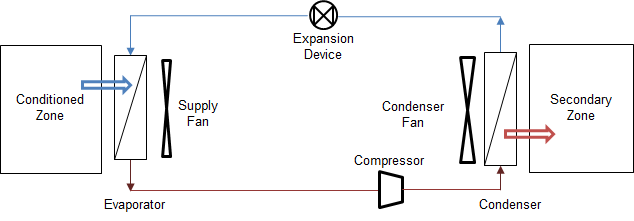
\includegraphics{media/image903.png}
\caption{}
\end{figure}

Figure: Schematic of DX System and heat pump in cooling operating mode

Applications of this technology include: inter-zone heat pump in NTED (Dixon, 2010), and PTAC or PTHP serving Offices attached to a Warehouse, where the office partially or fully enclosed by the warehouse and the condenser is inside the Warehouse. Heat rejected or extracted by the secondary DX coil installed in a secondary zone is estimated from the DX coil models and it is considered as internal gains of the secondary zone. The capacity and electric power input of the DX system and heat pumps are determined from the operating modes of the primary cooling or heating DX coils. Calculation of a secondary coil tracks the operating modes of the primary DX coil serving the primary conditioned zone(s). Currently allowed DX coil models are single speed, two speed and multi speed DX Systems and Heat Pumps. To model secondary DX coils the condenser type should be AirCooled. There is no need to specify the condenser air inlet node. The model uses zone air node as the secondary coil air inlet node. And the fuel type in multispeed DX coils should Electricity.

\textbf{Cooling Operating Mode}: the primary DX cooling coil of a DX system serving a primary zone is active and heat is rejected by the secondary coil (condenser) into a secondary zone. The secondary zone name is specified in DX cooling coil objects. This operating mode applies to a DX cooling system and cooling operating mode of air-to-air single and multi-speed heat pumps. Heat rejected by a secondary coil (condenser) calculated at each time step becomes internal gain of the secondary zone as shown in \protect\hyperlink{SecondaryCoilsFigure2}{Figure}. Whenever a secondary zone name is specified in DX cooling coil objects, the secondary DX coil model calculation is invoked. The only input field required to invoke the secondary DX coil in cooling operating model is to add a zone name in the input field \emph{Zone Name for Condenser Placement} in the DX cooling coil object.

\subsubsection{Field: Zone Name for Condenser Placement}\label{field-zone-name-for-condenser-placement-3}

This input field is name of a conditioned or unconditioned zone where the secondary coil (condenser) of DX system or a heat pump is to be placed. This is an optional input field specified only when user desires to reject the condenser heat into this zone. The heat rejected is modeled as sensible internal gain of a secondary zone.

\begin{figure}[htbp]
\centering
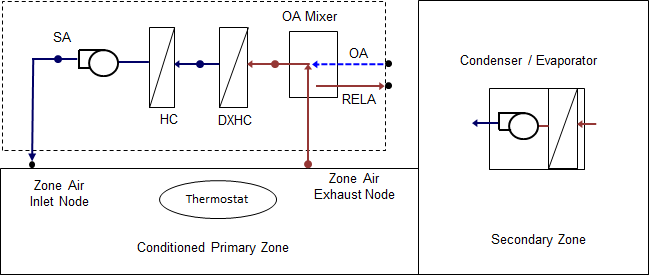
\includegraphics{media/image904.png}
\caption{}
\end{figure}

Figure: Schematic of DX system and secondary coil in cooling mode

Following is an example input for a single-speed cooling DX coil with secondary DX coil run option.

\begin{lstlisting}

Coil:Cooling:DX:SingleSpeed,
  Heat Pump ACDXCoil 1,    !- Name
  FanAndCoilAvailSched,    !- Availability Schedule Name
  autosize,                !- Gross Rated Total Cooling Capacity {W}
  autosize,                !- Gross Rated Sensible Heat Ratio
  3.0,                     !- Gross Rated Cooling COP {W/W}
  autosize,                !- Rated Air Flow Rate {m3/s}
  ,                        !- Rated Evaporator Fan Power Per Volume Flow Rate {W/(m3/s)}
  DX Cooling Coil Air Inlet Node,  !- Air Inlet Node Name
  Heating Coil Air Inlet Node,  !- Air Outlet Node Name
  HPACCoolCapFT,           !- Total Cooling Capacity Function of Temperature Curve Name
  HPACCoolCapFFF,          !- Total Cooling Capacity Function of Flow Fraction Curve Name
  HPACCOOLEIRFT,           !- Energy Input Ratio Function of Temperature Curve Name
  HPACCOOLEIRFFF,          !- Energy Input Ratio Function of Flow Fraction Curve Name
  HPACCOOLPLFFPLR,         !- Part Load Fraction Correlation Curve Name
  ,                        !- Nominal Time for Condensate Removal to Begin {s}
  ,   !- Ratio of Initial Moisture Evaporation Rate and Steady State Latent Capacity {dimensionless}
  ,                        !- Maximum Cycling Rate {cycles/hr}
  ,                        !- Latent Capacity Time Constant {s}
  ,                        !- Condenser Air Inlet Node Name
  AirCooled,               !- Condenser Type
  ,                        !- Evaporative Condenser Effectiveness {dimensionless}
  ,                        !- Evaporative Condenser Air Flow Rate {m3/s}
  ,                        !- Evaporative Condenser Pump Rated Power Consumption {W}
  ,                        !- Crankcase Heater Capacity {W}
  ,                 !- Maximum Outdoor Dry-Bulb Temperature for Crankcase Heater Operation {C}
  ,                        !- Supply Water Storage Tank Name
  ,                        !- Condensate Collection Water Storage Tank Name
  200,                     !- Basin Heater Capacity {W/K}
  ,                        !- Basin Heater Setpoint Temperature
  ,                        !- Basin Heater Operating Schedule Name
  ,                        !- Sensible Heat Ratio Function of Temperature Curve Name
  ,                        !- Sensible Heat Ratio Function of Flow Fraction Curve Name
  NORTH ZONE;              !- Zone Name for Condenser Placement
\end{lstlisting}

Following is an example input for a two-speed cooling DX coil with secondary DX coil run option.

\begin{lstlisting}

Coil:Cooling:DX:TwoSpeed,
  PSZ-AC_1:1_CoolC DXCoil, !- Name
  FanAndCoilAvailSched,    !- Availability Schedule Name
  AUTOSIZE,                !- High Speed Gross Rated Total Cooling Capacity {W}
  AUTOSIZE,                !- High Speed Rated Sensible Heat Ratio
  3.5,                     !- High Speed Gross Rated Cooling COP {W/W}
  AUTOSIZE,                !- High Speed Rated Air Flow Rate {m3/s}
  ,                        !- Unit Internal Static Air Pressure {Pa}
  DX Cooling Coil Air Inlet Node,     !- Air Inlet Node Name
  Heating Coil Air Inlet Node,        !- Air Outlet Node Name
  Measured_CoolCStandard10Ton_CapFT,!- Total Cooling Capacity Function of Temperature Curve Name
  Measured_CoolCStandard10Ton_CapFF,!- Total Cooling Capacity Function of Flow Fraction Curve Name
  Measured_CoolCStandard10Ton_EIRFT,  !- Energy Input Ratio Function of Temperature Curve Name
  Measured_CoolCStandard10Ton_EIRFFF, !- Energy Input Ratio Function of Flow Fraction Curve Name
  No_PLR_Degredation,      !- Part Load Fraction Correlation Curve Name
  AUTOSIZE,                !- Low Speed Gross Rated Total Cooling Capacity {W}
  AUTOSIZE,                !- Low Speed Gross Rated Sensible Heat Ratio
  3.3,                     !- Low Speed Gross Rated Cooling COP {W/W}
  AUTOSIZE,                !- Low Speed Rated Air Flow Rate {m3/s}
  MeasuredLowSpeedCoolCapLSFT,!- Low Speed Total Cooling Capacity Function of Temperature Curve Name
  MeasuredLowSpeedCoolEIRLSFT,!- Low Speed Energy Input Ratio Function of Temperature Curve Name
  ,                              !- Condenser Air Inlet Node Name
  AirCooled,               !- Condenser Type
  ,                        !- High Speed Evaporative Condenser Effectiveness {dimensionless}
  ,                        !- High Speed Evaporative Condenser Air Flow Rate {m3/s}
  ,                        !- High Speed Evaporative Condenser Pump Rated Power Consumption {W}
  ,                        !- Low Speed Evaporative Condenser Effectiveness {dimensionless}
  ,                        !- Low Speed Evaporative Condenser Air Flow Rate {m3/s}
  ,                        !- Low Speed Evaporative Condenser Pump Rated Power Consumption {W}
  ,                        !- Supply Water Storage Tank Name
  ,                        !- Condensate Collection Water Storage Tank Name
  ,                        !- Basin Heater Capacity {W/K}
  ,                        !- Basin Heater Setpoint Temperature {C}
  ,                        !- Basin Heater Operating Schedule Name
  ,     !- Sensible Heat Ratio Function of Temperature Curve Name
  ,     !- Sensible Heat Ratio Function of Flow Fraction Curve Name
  ,     !- Low Speed Sensible Heat Ratio Function of Temperature Curve Name
  ,     !- Low Speed Sensible Heat Ratio Function of Flow Fraction Curve Name
  NORTH ZONE;              !- Zone Name for Condenser Placement
\end{lstlisting}

Following is an example input for a multi-speed cooling DX coil with secondary DX coil run option.

\begin{lstlisting}

Coil:Cooling:DX:MultiSpeed,
  Heat Pump ACDXCoil 1,    !- Name
  FanAndCoilAvailSched,    !- Availability Schedule Name
  DX Cooling Coil Air Inlet Node,  !- Air Inlet Node Name
  Heating Coil Air Inlet Node,  !- Air Outlet Node Name
  Outdoor Condenser Air Node,  !- Condenser Air Inlet Node Name
  AirCooled,               !- Condenser Type
  ,                        !- Supply Water Storage Tank Name
  ,                        !- Condensate Collection Water Storage Tank Name
  No,                      !- Apply Part Load Fraction to Speeds Greater than 1
  No,                      !- Apply Latent Degradation to Speeds Greater than 1
  200.0,                   !- Crankcase Heater Capacity {W}
  10.0,           !- Maximum Outdoor Dry-Bulb Temperature for Crankcase Heater Operation {C}
  ,                        !- Basin Heater Capacity {W/K}
  ,                        !- Basin Heater Setpoint Temperature {C}
  ,                        !- Basin Heater Operating Schedule Name
  Electricity,             !- Fuel Type
  4,                       !- Number of Speeds
  autosize,                !- Speed 1 Gross Rated Total Cooling Capacity {W}
  autosize,                !- Speed 1 Gross Rated Sensible Heat Ratio
  3.0,                     !- Speed 1 Gross Rated Cooling COP {W/W}
  autosize,                !- Speed 1 Rated Air Flow Rate {m3/s}
  453.3,                   !- Rated Evaporator Fan Power Per Volume Flow Rate {W/(m3/s)}
  HPACCoolCapFT Speed 1,   !- Speed 1 Total Cooling Capacity Function of Temperature Curve Name
  HPACCoolCapFF Speed 1, !- Speed 1 Total Cooling Capacity Function of Flow Fraction Curve Name
  HPACCOOLEIRFT Speed 1,   !- Speed 1 Energy Input Ratio Function of Temperature Curve Name
  HPACCOOLEIRFF Speed 1,   !- Speed 1 Energy Input Ratio Function of Flow Fraction Curve Name
  HPACCOOLPLFFPLR Speed 1, !- Speed 1 Part Load Fraction Correlation Curve Name
  1000.0,                  !- Speed 1 Nominal Time for Condensate Removal to Begin {s}
  1.5,  !- Speed 1 Ratio of Initial Moisture Evaporation Rate and Steady State Latent Capacity {dimensionless}
  3.0,                     !- Speed 1 Maximum Cycling Rate {cycles/hr}
  45.0,                    !- Speed 1 Latent Capacity Time Constant {s}
  0.2,                     !- Speed 1 Rated Waste Heat Fraction of Power Input {dimensionless}
  HAPCCoolWHFT Speed 1,    !- Speed 1 Waste Heat Function of Temperature Curve Name
  0.9,                     !- Speed 1 Evaporative Condenser Effectiveness {dimensionless}
  autosize,                !- Speed 1 Evaporative Condenser Air Flow Rate {m3/s}
  50,                      !- Speed 1 Rated Evaporative Condenser Pump Power Consumption {W}
  autosize,                !- Speed 2 Gross Rated Total Cooling Capacity {W}
  autosize,                !- Speed 2 Gross Rated Sensible Heat Ratio
  3.0,                     !- Speed 2 Gross Rated Cooling COP {W/W}
  autosize,                !- Speed 2 Rated Air Flow Rate {m3/s}
  523.3,                   !- Rated Evaporator Fan Power Per Volume Flow Rate {W/(m3/s)}
  HPACCoolCapFT Speed 2,   !- Speed 2 Total Cooling Capacity Function of Temperature Curve Name
  HPACCoolCapFF Speed 2, !- Speed 2 Total Cooling Capacity Function of Flow Fraction Curve Name
  HPACCOOLEIRFT Speed 2,   !- Speed 2 Energy Input Ratio Function of Temperature Curve Name
  HPACCOOLEIRFF Speed 2,   !- Speed 2 Energy Input Ratio Function of Flow Fraction Curve Name
  HPACCOOLPLFFPLR Speed 1, !- Speed 2 Part Load Fraction Correlation Curve Name
  1000.0,                  !- Speed 2 Nominal Time for Condensate Removal to Begin {s}
  1.5,  !- Speed 2 Ratio of Initial Moisture Evaporation Rate and steady state Latent Capacity {dimensionless}
  3.0,                     !- Speed 2 Maximum Cycling Rate {cycles/hr}
  45.0,                    !- Speed 2 Latent Capacity Time Constant {s}
  0.2,                     !- Speed 2 Rated Waste Heat Fraction of Power Input {dimensionless}
  HAPCCoolWHFT Speed 2,    !- Speed 2 Waste Heat Function of Temperature Curve Name
  0.9,                     !- Speed 2 Evaporative Condenser Effectiveness {dimensionless}
  autosize,                !- Speed 2 Evaporative Condenser Air Flow Rate {m3/s}
  60,                      !- Speed 2 Rated Evaporative Condenser Pump Power Consumption {W}
  autosize,                !- Speed 3 Gross Rated Total Cooling Capacity {W}
  autosize,                !- Speed 3 Gross Rated Sensible Heat Ratio
  3.0,                     !- Speed 3 Gross Rated Cooling COP {W/W}
  autosize,                !- Speed 3 Rated Air Flow Rate {m3/s}
  573.3,                   !- Rated Evaporator Fan Power Per Volume Flow Rate {W/(m3/s)}
  HPACCoolCapFT Speed 3,   !- Speed 3 Total Cooling Capacity Function of Temperature Curve Name
  HPACCoolCapFF Speed 3, !- Speed 3 Total Cooling Capacity Function of Flow Fraction Curve Name
  HPACCOOLEIRFT Speed 3,   !- Speed 3 Energy Input Ratio Function of Temperature Curve Name
  HPACCOOLEIRFF Speed 3,   !- Speed 3 Energy Input Ratio Function of Flow Fraction Curve Name
  HPACCOOLPLFFPLR Speed 1, !- Speed 3 Part Load Fraction Correlation Curve Name
  1000.0,                  !- Speed 3 Nominal Time for Condensate Removal to Begin {s}
  1.5, !- Speed 3 Ratio of Initial Moisture Evaporation Rate and steady state Latent Capacity {dimensionless}
  3.0,                     !- Speed 3 Maximum Cycling Rate {cycles/hr}
  45.0,                    !- Speed 3 Latent Capacity Time Constant {s}
  0.2,                     !- Speed 3 Rated Waste Heat Fraction of Power Input {dimensionless}
  HAPCCoolWHFT Speed 3,    !- Speed 3 Waste Heat Function of Temperature Curve Name
  0.9,                     !- Speed 3 Evaporative Condenser Effectiveness {dimensionless}
  autosize,                !- Speed 3 Evaporative Condenser Air Flow Rate {m3/s}
  80,                      !- Speed 3 Rated Evaporative Condenser Pump Power Consumption {W}
  autosize,                !- Speed 4 Gross Rated Total Cooling Capacity {W}
  autosize,                !- Speed 4 Gross Rated Sensible Heat Ratio
  3.0,                     !- Speed 4 Gross Rated Cooling COP {W/W}
  autosize,                !- Speed 4 Rated Air Flow Rate {m3/s}
  673.3,                   !- Rated Evaporator Fan Power Per Volume Flow Rate {W/(m3/s)}
  HPACCoolCapFT Speed 4,   !- Speed 4 Total Cooling Capacity Function of Temperature Curve Name
  HPACCoolCapFF Speed 4, !- Speed 4 Total Cooling Capacity Function of Flow Fraction Curve Name
  HPACCOOLEIRFT Speed 4,   !- Speed 4 Energy Input Ratio Function of Temperature Curve Name
  HPACCOOLEIRFF Speed 4,   !- Speed 4 Energy Input Ratio Function of Flow Fraction Curve Name
  HPACCOOLPLFFPLR Speed 1, !- Speed 4 Part Load Fraction Correlation Curve Name
  1000.0,                  !- Speed 4 Nominal Time for Condensate Removal to Begin {s}
  1.5, !- Speed 4 Ratio of Initial Moisture Evaporation Rate and steady state Latent Capacity {dimensionless}
  3.0,                     !- Speed 4 Maximum Cycling Rate {cycles/hr}
  45.0,                    !- Speed 4 Latent Capacity Time Constant {s}
  0.2,                     !- Speed 4 Rated Waste Heat Fraction of Power Input {dimensionless}
  HAPCCoolWHFT Speed 4,    !- Speed 4 Waste Heat Function of Temperature Curve Name
  0.9,                     !- Speed 4 Evaporative Condenser Effectiveness {dimensionless}
  autosize,                !- Speed 4 Evaporative Condenser Air Flow Rate {m3/s}
  100,                     !- Speed 4 Rated Evaporative Condenser Pump Power Consumption {W}
  NORTH ZONE;              !- Zone Name for Condenser Placement
\end{lstlisting}

\textbf{Heating Operating Mode}: When a heat pump operates in heating mode then energy is extracted from the secondary zone. Total energy extracted from a secondary zone may contain sensible and latent components. The secondary coil (evaporator) model checks for the coil inlet and outlet air condition to determine if dehumidification has occurred. The sensible and latent split of the energy extracted is done using a user specified rated sensible heat ratio (SHR) and SHR modifier curves for temperature and secondary air flow fraction. If the coil operation is dry, then the SHR is set to 1.0. In addition, the model assumes that condensed water is drained to the outside. If defrosting operation is on, then the defrosting melts the frost and the liquid water from the collecting pan is drained to the outside. Thus, defrosting energy is not included in the zone energy balance. The six optioal input fields required in the DX heating coils are the following. This object is extensible by repeating the last five input fields depending on the speed of the heating DX coil:

\subsubsection{Field: Zone Name for Evaporator Placement}\label{field-zone-name-for-evaporator-placement-2}

This input field is name of a conditioned or unconditioned zone where the secondary coil (evaporator) of a heat pump is installed. This is an optional input field specified only when user desires to extract heat from the zone via secondary coil. Heat extracted is modeled as internal gain. If the primary DX system is a heat pump, then the zone name should be the same as the zone name specified for placing the secondary cooling DX coil.

\subsubsection{Field: Speed Secondary Coil Air Flow Rate}\label{field-speed-secondary-coil-air-flow-rate}

This input value is the secondary coil (evaporator) air flow rate when the heat pump is working in heating mode or the secondary coil (condenser) air flow rate when the heat pump is working in cooling mode. This input field is auto-sizable.

\subsubsection{Field: Speed Secondary Coil Fan Flow Scaling Factor}\label{field-speed-secondary-coil-fan-flow-scaling-factor}

This input field is scaling factor for autosizing the secondary DX coil fan flow rate. The secondary air flow rate is determined by multiplying the primary DX coil rated air flow rate by the fan flow scaling factor. Default value is 1.25. If the secondary coil fan flow rate is not autosized, then the secondary coil fan flow scaling factor is set to 1.0.

\subsubsection{Field: Speed Nominal Sensible Heat Ratio of Secondary Coil}\label{field-speed-nominal-sensible-heat-ratio-of-secondary-coil}

This input value is the nominal sensible heat ratio used to split the heat extracted by a secondary DX coil (evaporator) of a heat pump into sensible and latent components. This is an optional input field. If this input field is left blank, then pure sensible internal heat gain is assumed, i.e., sensible heat ratio of 1.0.

\subsubsection{Field: Speed Sensible Heat Ratio Modifier Function of Temperature Curve Name}\label{field-speed-sensible-heat-ratio-modifier-function-of-temperature-curve-name}

This input field is name of sensible heat ratio modifier biquadratic curve. The value of this curve modifies the nominal sensible heat ratio for current time step depending on the secondary zone air node wet-bulb temperature and the heating DX coil entering air dry-bulb temperature. This is an optional input field. If this input field is left blank, then the nominal sensible heat ratio modifier curve value for temperature is set to 1.0.

\subsubsection{Field: Speed Sensible Heat Ratio Modifier Function of Flow Fraction Curve Name}\label{field-speed-sensible-heat-ratio-modifier-function-of-flow-fraction-curve-name}

This input field is name of sensible heat ratio modifier curve as function of secondary air flow fraction. The value of this curve modifies the nominal sensible heat ratio for current time step depending on the secondary coil air flow fraction. This is an optional input field. If this input field is left blank, then the sensible heat ratio modifier curve value for flow fraction is set to 1.0.

Following is an example input for a single-speed heating DX coil with secondary DX coil run option.

\begin{lstlisting}

Coil:Heating:DX:SingleSpeed,
  Heat Pump DX Heating Coil 1,  !- Name
  FanAndCoilAvailSched,    !- Availability Schedule Name
  autosize,                !- Gross Rated Heating Capacity {W}
  2.75,                    !- Gross Rated Heating COP {W/W}
  autosize,                !- Rated Air Flow Rate {m3/s}
  ,                        !- Rated Supply Fan Power Per Volume Flow Rate {W/(m3/s)}
  Heating Coil Air Inlet Node,  !- Air Inlet Node Name
  SuppHeating Coil Air Inlet Node,  !- Air Outlet Node Name
  HPACHeatCapFT,           !- Heating Capacity Function of Temperature Curve Name
  HPACHeatCapFFF,          !- Heating Capacity Function of Flow Fraction Curve Name
  HPACHeatEIRFT,           !- Energy Input Ratio Function of Temperature Curve Name
  HPACHeatEIRFFF,          !- Energy Input Ratio Function of Flow Fraction Curve Name
  HPACCOOLPLFFPLR,         !- Part Load Fraction Correlation Curve Name
  ,                        !- Defrost Energy Input Ratio Function of Temperature Curve Name
  -5.0,                     !- Minimum Outdoor Dry-Bulb Temperature for Compressor Operation {C}
  ,                        !- Outdoor Dry-Bulb Temperature to Turn On Compressor {C}
  5.0,                     !- Maximum Outdoor Dry-Bulb Temperature for Defrost Operation {C}
  200.0,                   !- Crankcase Heater Capacity {W}
  10.0,             !- Maximum Outdoor Dry-Bulb Temperature for Crankcase Heater Operation {C}
  Resistive,               !- Defrost Strategy
  TIMED,                   !- Defrost Control
  0.166667,                !- Defrost Time Period Fraction
  autosize,                !- Resistive Defrost Heater Capacity {W}
  4,                       !- Region number for calculating HSPF
  ,                        !- Evaporator Air Inlet Node Name
  NORTH ZONE,              !- Zone Name for Evaporator Placement
  autosize,                !- Secondary Coil Air Flow Rate
  1.5,                     !- Secondary Coil Fan Flow Scaling Factor
  0.9,                     !- Nominal Sensible Heat Ratio of Secondary Coil
  DXSecondaryCoilSHRFT,    !- Sensible Heat Ratio Modifier Function of Temperature Curve Name
  DXSecondaryCoilSHRFFF;   !- Sensible Heat Ratio Function of Flow Fraction Curve Name
\end{lstlisting}

Following is an example input for a multi-speed heating DX coil with secondary DX coil run option.

\begin{lstlisting}

Coil:Heating:DX:MultiSpeed,
  Heat Pump DX Heating Coil 1,  !- Name
  FanAndCoilAvailSched,    !- Availability Schedule Name
  Heating Coil Air Inlet Node,  !- Air Inlet Node Name
  SuppHeating Coil Air Inlet Node,  !- Air Outlet Node Name
  -8.0,                    !- Minimum Outdoor Dry-Bulb Temperature for Compressor Operation {C}
  -5.0,                    !- Outdoor Dry-Bulb Temperature to Turn On Compressor {C}
  200.0,                   !- Crankcase Heater Capacity {W}
  10.0,              !- Maximum Outdoor Dry-Bulb Temperature for Crankcase Heater Operation {C}
  HPACDefrostCAPFT,        !- Defrost Energy Input Ratio Function of Temperature Curve Name
  7.22,                    !- Maximum Outdoor Dry-Bulb Temperature for Defrost Operation {C}
  ReverseCycle,            !- Defrost Strategy
  timed,                   !- Defrost Control
  0.058333,                !- Defrost Time Period Fraction
  autosize,                !- Resistive Defrost Heater Capacity {W}
  No,                      !- Apply Part Load Fraction to Speeds Greater than 1
  Electricity,             !- Fuel Type
  4,                       !- Region number for Calculating HSPF
  4,                       !- Number of Speeds
  autosize,                !- Speed 1 Gross Rated Heating Capacity {W}
  2.75,                    !- Speed 1 Gross Rated Heating COP {W/W}
  autosize,                !- Speed 1 Rated Air Flow Rate {m3/s}
  345.0,                   !- Speed 1 Rated Supply Air Fan Power Per Volume Flow Rate {W/(m3/s)}
  HPACHeatCapFT Speed 1,   !- Speed 1 Heating Capacity Function of Temperature Curve Name
  HPACHeatCapFF Speed 1,   !- Speed 1 Heating Capacity Function of Flow Fraction Curve Name
  HPACHeatEIRFT Speed 1,   !- Speed 1 Energy Input Ratio Function of Temperature Curve Name
  HPACHeatEIRFF Speed 1,   !- Speed 1 Energy Input Ratio Function of Flow Fraction Curve Name
  HPACHeatPLFFPLR Speed 1, !- Speed 1 Part Load Fraction Correlation Curve Name
  0.2,                     !- Speed 1 Rated Waste Heat Fraction of Power Input {dimensionless}
  HAPCHeatWHFT Speed 1,    !- Speed 1 Waste Heat Function of Temperature Curve Name
  autosize,                !- Speed 2 Gross Rated Heating Capacity {W}
  2.75,                    !- Speed 2 Gross Rated Heating COP {W/W}
  autosize,                !- Speed 2 Rated Air Flow Rate {m3/s}
  425.0,                   !- Speed 2 Rated Supply Air Fan Power Per Volume Flow Rate {W/(m3/s)}
  HPACHeatCapFT Speed 2,   !- Speed 2 Heating Capacity Function of Temperature Curve Name
  HPACHeatCapFF Speed 2,   !- Speed 2 Heating Capacity Function of Flow Fraction Curve Name
  HPACHeatEIRFT Speed 2,   !- Speed 2 Energy Input Ratio Function of Temperature Curve Name
  HPACHeatEIRFF Speed 2,   !- Speed 2 Energy Input Ratio Function of Flow Fraction Curve Name
  HPACHeatPLFFPLR Speed 2, !- Speed 2 Part Load Fraction Correlation Curve Name
  0.2,                     !- Speed 2 Rated Waste Heat Fraction of Power Input {dimensionless}
  HAPCHeatWHFT Speed 2,    !- Speed 2 Waste Heat Function of Temperature Curve Name
  autosize,                !- Speed 3 Gross Rated Heating Capacity {W}
  2.75,                    !- Speed 3 Gross Rated Heating COP {W/W}
  autosize,                !- Speed 3 Rated Air Flow Rate {m3/s}
  525.0,                   !- Speed 3 Rated Supply Air Fan Power Per Volume Flow Rate {W/(m3/s)}
  HPACHeatCapFT Speed 3,   !- Speed 3 Heating Capacity Function of Temperature Curve Name
  HPACHeatCapFF Speed 3,   !- Speed 3 Heating Capacity Function of Flow Fraction Curve Name
  HPACHeatEIRFT Speed 3,   !- Speed 3 Energy Input Ratio Function of Temperature Curve Name
  HPACHeatEIRFF Speed 3,   !- Speed 3 Energy Input Ratio Function of Flow Fraction Curve Name
  HPACHeatPLFFPLR Speed 3, !- Speed 3 Part Load Fraction Correlation Curve Name
  0.2,                     !- Speed 3 Rated Waste Heat Fraction of Power Input {dimensionless}
  HAPCHeatWHFT Speed 3,    !- Speed 3 Waste Heat Function of Temperature Curve Name
  autosize,                !- Speed 4 Gross Rated Heating Capacity {W}
  2.75,                    !- Speed 4 Gross Rated Heating COP {W/W}
  autosize,                !- Speed 4 Rated Air Flow Rate {m3/s}
  673.0,                   !- Speed 4 Rated Supply Air Fan Power Per Volume Flow Rate {W/(m3/s)}
  HPACHeatCapFT Speed 4,   !- Speed 4 Heating Capacity Function of Temperature Curve Name
  HPACHeatCapFF Speed 4,   !- Speed 4 Heating Capacity Function of Flow Fraction Curve Name
  HPACHeatEIRFT Speed 4,   !- Speed 4 Energy Input Ratio Function of Temperature Curve Name
  HPACHeatEIRFF Speed 4,   !- Speed 4 Energy Input Ratio Function of Flow Fraction Curve Name
  HPACHeatPLFFPLR Speed 4, !- Speed 4 Part Load Fraction Correlation Curve Name
  0.2,                     !- Speed 4 Rated Waste Heat Fraction of Power Input {dimensionless}
  HAPCHeatWHFT Speed 4,    !- Speed 4 Waste Heat Function of Temperature Curve Name
  NORTH ZONE,              !- Zone Name for Evaporator Placement
  autosize,                !- Speed 1 Secondary Coil Air Flow Rate
  1.5,                     !- Speed 1 Secondary Coil Fan Flow Scaling Factor
  0.9,                     !- Speed 1 Nominal Sensible Heat Ratio of Secondary Coil
  DXSecondaryCoilSHRFT,!- Speed 1 Sensible Heat Ratio Modifier Function of Temperature Curve Name
  DXSecondaryCoilSHRFFF,   !- Speed 1 Sensible Heat Ratio Function of Flow Fraction Curve Name
  autosize,                !- Speed 2 Secondary Coil Air Flow Rate
  1.5,                     !- Speed 2 Secondary Coil Fan Flow Scaling Factor
  0.9,                     !- Speed 2 Nominal Sensible Heat Ratio of Secondary Coil
  DXSecondaryCoilSHRFT,!- Speed 2 Sensible Heat Ratio Modifier Function of Temperature Curve Name
  DXSecondaryCoilSHRFFF,   !- Speed 2 Sensible Heat Ratio Function of Flow Fraction Curve Name
  autosize,                !- Speed 3 Secondary Coil Air Flow Rate
  1.5,                     !- Speed 3 Secondary Coil Fan Flow Scaling Factor
  0.9,                     !- Speed 3 Nominal Sensible Heat Ratio of Secondary Coil
  DXSecondaryCoilSHRFT,!- Speed 3 Sensible Heat Ratio Modifier Function of Temperature Curve Name
  DXSecondaryCoilSHRFFF,   !- Speed 3 Sensible Heat Ratio Function of Flow Fraction Curve Name
  autosize,                !- Speed 4 Secondary Coil Air Flow Rate
  1.5,                     !- Speed 4 Secondary Coil Fan Flow Scaling Factor
  0.9,                     !- Speed 4 Nominal Sensible Heat Ratio of Secondary Coil
  DXSecondaryCoilSHRFT,!- Speed 4 Sensible Heat Ratio Modifier Function of Temperature Curve Name
  DXSecondaryCoilSHRFFF;   !- Speed 4 Sensible Heat Ratio Function of Flow Fraction Curve Name
\end{lstlisting}

\subsection{Secondary DX Coil Output}\label{secondary-dx-coil-output}

\begin{itemize}
\item
  HVAC, Average, Secondary Coil Heat Rejection Rate {[}W{]}
\item
  HVAC, Average, Secondary Coil Total Heat Removal Rate {[}W{]}
\item
  HVAC, Average, Secondary Coil Sensible Heat Removal Rate {[}W{]}
\item
  HVAC, Average, Secondary Coil Latent Heat Removal Rate {[}W{]}
\item
  HVAC, Average, Secondary Coil Sensible Heat Ratio {[]}
\item
  HVAC, Average, Secondary Coil Compressor Part Load Ratio {[]}
\end{itemize}

\subsubsection{Secondary Coil Heat Rejection Rate {[}W{]}}\label{secondary-coil-heat-rejection-rate-w}

This is the sensible heat rejected to a zone by a secondary DX coil (condenser) in Watts. This is sum of the total cooling rate of a DX cooling coil and cooling electric power of the primary DX coil. This heat is applied as an internal gain to the secondary zone where the condenser is installed.

\subsubsection{Secondary Coil Total Heat Removal Rate {[}W{]}}\label{secondary-coil-total-heat-removal-rate-w}

This is the total energy removed from a a zone by a secondary DX coil (evaporator) in Watts. This is the total heating rate of the primary DX cooling coil minus the heating electric power of the primary DX coil. This heat is extracted from the secondary zone when the heat pump is operating in heating mode. The negative sign indicate that heat is removed from the zone.

\subsubsection{Secondary Coil Sensible Heat Removal Rate {[}W{]}}\label{secondary-coil-sensible-heat-removal-rate-w}

This is the sensible heat removed from a a zone by a secondary DX coil (evaporator) in Watts. This is determined by multiplying the total heat removed with sensible heat ratio of the secondary coil. This heat is extracted from the secondary zone when the heat pump is operating in heating mode. The negative sign indicate that sensible heat is removed from the zone.

\subsubsection{Secondary Coil Latent Heat Removal Rate {[}W{]}}\label{secondary-coil-latent-heat-removal-rate-w}

This is the latent heat removed from a a zone by a secondary DX coil (evaporator) in Watts. This is the difference between the total heat removal rate and the sensible heat remobal rate of the secondary coil. This heat is extracted from the secondary zone when the heat pump is operating in heating mode. The negative sign indicate that moisture is removed from the zone.

\subsubsection{Secondary Coil Sensible Heat Ratio {[]}}\label{secondary-coil-sensible-heat-ratio}

This is the operating sensible heat ratio the secondary DX coil (condenser) when the heat pump is operating in heating mode.

\subsubsection{Secondary Coil Compressor Part Load Ratio {[]}}\label{secondary-coil-compressor-part-load-ratio}

This is the compressor part load ratio when the heat pump is operating in heating mode and the secondary coil is extracting heat from a zone where the coil is installed. The secondary coil DX coil compressor part load ratio can be different from the primary DX coil compressor part load ratio in that the later may include the defrosting load.

Reference: Dixon, Erin Elizabeth, ``Energy Model Development and Heating Energy Investigation of the Nested Thermal Envelope Design (NTED (tm))'' (2010). Theses and dissertations. Paper 974.
